%% -*- Mode:TeX; Fonts:(hl12fb) -*-
%% *-* File: /usr/local/gbbopen/doc-source/tutorial.tex *-*
%% *-* Last-Edit: Sun Apr 27 11:30:23 2008; Edited-By: cork *-*
%% *-* Machine: cyclone.cs.umass.edu *-*

%% Copyright (C) 2005-2008, Dan Corkill <corkill@GBBopen.org>
%% Part of the GBBopen Project (see LICENSE for license information).
%%
%% ========================================================================
%%  The LaTeX and hyperlatex code used in producing GBBopen documentation
%%  is placed under and covered by the GBBopen software license that 
%%  accompanies each GBBopen distribution and is also available at
%%  http://GBBopen.org/downloads/LICENSE. 
%% ========================================================================
%%
%%  Note: To keep both LaTeX and hyperlatex happy with indexing, index
%%        commands must be positioned with care (including the use of
%%        % after all entries).  Follow the placement used here to
%%        minimize the creation of anchors by hyperlatex.  Indexes
%%        should only be placed at locations where an inserted &nbsp; 
%%        anchor does not visibly affect the html layout.
%%
%%        \indexit doesn't play well with @\xxx{} formating, so use
%%        the basic \index{...|itidx} rather than \indexit shorthand.
        
\documentclass[10pt,twoside,english,pdftex]{article} 
\usepackage{hyperlatex}
\usepackage{color}
\usepackage{makeidx}
\T\usepackage{atbeginend}
%\T\usepackage{palatino}
\T\usepackage{newcent}
% Use smaller TT font throughout
\W\begin{iftex}
  \makeatletter
  \DeclareRobustCommand\smallttfamily
  {\not@math@alphabet\ttfamily\mathtt
    \fontfamily\ttdefault\small\selectfont}
  \makeatother
\W\end{iftex}
\T\usepackage{fancyhdr}
\W\usepackage{frames}
%% Req'd for pdflatex -- note use epstopdf to convert eps figures;
%%                       ps2pdf won't create correct bounding boxes
\T\newif\ifpdf\ifx\pdfoutput\undefined\pdffalse\else\pdfoutput=1\pdftrue\fi
\T\newcommand{\pdfgraphics}{\ifpdf\DeclareGraphicsExtensions{.pdf,.jpg}\else\fi}
\T\usepackage{graphicx}

\newcommand{\docname}{Tutorial}

%% -*- Mode:TeX; Fonts:(hl12fb) -*-
%% *-* File: /home/gbbopen/current/doc-source/test-common.tex *-*
%% *-* Last-Edit: Thu Dec 28 06:25:02 2006; Edited-By: cork *-*
%% *-* Machine: ruby.corkills.org *-*

%% Copyright (C) 2003-2006, Dan Corkill <corkill@GBBopen.org>
%% Part of the GBBopen Project (see LICENSE for license information).
%%
%% ========================================================================
%%  The LaTeX and hyperlatex code used in producing GBBopen documentation
%%  is placed under and covered by  the GBBopen software license that 
%%  accompanies each GBBopen distribution and is also available at
%%  http://GBBopen.org/downloads/LICENSE. 
%% ========================================================================

\newcommand{\noargs}{$<$no arguments$>$}
\T\newcommand{\bkslash}{$\backslash$}
\W\newcommand{\bkslash}{\backslash}
\T\newcommand{\vbar}{$|$}
\W\newcommand{\vbar}{|}
\T\newcommand{\superstar}{\raisebox{2pt}{*}}
\W\newcommand{\superstar}{*}
\T\newcommand{\superplus}{\raisebox{4pt}{+}}
\W\newcommand{\superplus}{\xml{sup}+\xml{/sup}}
\definecolor{rulegray}{gray}{.75}
\definecolor{darkergray}{gray}{.55}
\definecolor{caution}{rgb}{.8,.6,.0}

%% ----------------------------------------------------------------------------
%%   Margins

\T\headsep 26pt
\T\footskip 36pt
\T\topmargin -40pt
\T\oddsidemargin 0pt
\T\evensidemargin 0pt
\T\textwidth 470pt
\T\textheight 630pt

%% ----------------------------------------------------------------------------
%%   Headings/Footings

\W\begin{iftex}
\fancyhf{} % clear all
\fancyhead[er,ol]{\textcolor{darkergray}{\rightmark}}
\fancyfoot[er,ol]{\textcolor{darkergray}{\runningtitle}
                \\\textcolor{darkergray}{\nouppercase{\leftmark}}}
\fancyfoot[el,or]{~\\\thepage}

\makeatletter

%% from fancyhdr
\def\ps@fancy{%
\@ifundefined{@chapapp}{\let\@chapapp\chaptername}{}%for amsbook
%
% Define \MakeUppercase for old LaTeXen.
% Note: we used \def rather than \let, so that \let\uppercase\relax (from
% the version 1 documentation) will still work.
%
\@ifundefined{MakeUppercase}{\def\MakeUppercase{\uppercase}}{}%
\@ifundefined{chapter}{\def\sectionmark##1{\markboth
{\ifnum \c@secnumdepth>\z@
 \thesection\hskip 1em\relax \fi ##1}{}}%
\def\subsectionmark##1{\markboth {\ifnum \c@secnumdepth >\@ne
 \thesubsection\hskip 1em\relax \fi ##1}{}}}%
{\def\chaptermark##1{\markboth {\MakeUppercase{\ifnum \c@secnumdepth>\m@ne
 \@chapapp\ \thechapter. \ \fi ##1}}{}}%
\def\sectionmark##1{\markboth{\ifnum \c@secnumdepth >\z@
 \thesection. \ \fi ##1}{}}}%
\ps@@fancy
\gdef\ps@fancy{\@fancyplainfalse\ps@@fancy}%
\ifdim\headwidth<0sp
    \global\advance\headwidth123456789sp\global\advance\headwidth\textwidth
\fi}
\def\ps@fancyplain{\ps@fancy \let\ps@plain\ps@plain@fancy}
\def\ps@plain@fancy{\@fancyplaintrue\ps@@fancy}
\let\ps@@empty\ps@empty

%% mod of \headrule from fancyhdr.sty (to make rule gray):
\def\headrule{{\if@fancyplain\let\headrulewidth\plainheadrulewidth\fi
    \vskip-0.8\baselineskip % tighten rule to \rightmark
    \textcolor{rulegray}{\hrule\@height\headrulewidth\@width\headwidth 
    \vskip-\headrulewidth}}}

%% mod of \ps@@fancy from fancyhdr.sty:
\def\ps@fancybottom{%
\def\@mkboth{\protect\markboth}%
\def\@oddhead{}%
\def\@oddfoot{\@fancyfoot\fancy@Oolf\f@ncyolf\f@ncyocf\f@ncyorf\fancy@Oorf}%
\def\@evenhead{}%
\def\@evenfoot{\@fancyfoot\fancy@Oelf\f@ncyelf\f@ncyecf\f@ncyerf\fancy@Oerf}%
}
\makeatother
\W\end{iftex}

\T\begin{ifhtml}
\newcommand\entities{\textbf{\large Entities}}
\T\end{ifhtml}

%% ----------------------------------------------------------------------------
%%  LaTeX Modifications

\W\begin{iftex}
\makeatletter

% article.cls
\renewcommand\@idxitem{\par\hangindent 30\p@}
\renewcommand\subitem{\@idxitem \hspace*{10\p@}}
\renewcommand\subsubitem{\@idxitem \hspace*{20\p@}}
% ppar
\newcommand{\ppar}[1]{\paragraph{#1}~\\[0.5\baselineskip]%
  \T\addcontentsline{toc}{subsubsection}{{#1}}
}
% Tighten up example environment (uses atbeginend.sty):
\AfterBegin{example}{\vspace*{-0.8\baselineskip}}

% fndocsec
\newcommand{\fndocsec}{\@startsection{subparagraph}{5}{\z@}%
                          {1.25ex \@plus1ex \@minus.1ex}%
                          {-1em}%
                          {\normalfont\large\sffamily\bfseries}}
% from article.cls - Increase TOC font for sections and subsections
\renewcommand*\l@section[2]{%
  \ifnum \c@tocdepth >\z@
    \addpenalty\@secpenalty
    \addvspace{1.0em \@plus\p@}%
    \setlength\@tempdima{2.0em}%
    \begingroup
      \parindent \z@ \rightskip \@pnumwidth
      \parfillskip -\@pnumwidth
      \leavevmode \bfseries
      \advance\leftskip\@tempdima
      \hskip -\leftskip
      {\large #1}\nobreak\hfil \nobreak\hb@xt@\@pnumwidth{\hss\large #2}\par
    \endgroup
    \addvspace{.5em \@plus\p@}%
  \fi}
\renewcommand*\l@subsection[2]{%
  \ifnum \c@tocdepth >\z@
    \addpenalty\@secpenalty
    \addvspace{0.4em \@plus\p@}%
    \setlength\@tempdima{2.3em}%
    \begingroup
      \parindent \z@ \rightskip \@pnumwidth
      \parfillskip -\@pnumwidth
      \leavevmode \bfseries
      \advance\leftskip\@tempdima
      \hskip -\leftskip
      #1\nobreak\hfil \nobreak\hb@xt@\@pnumwidth{\hss #2}\par
    \endgroup
    \addvspace{.2em \@plus\p@}%
  \fi}
% from article.cls - Decrease TOC leftmargin for subsubsections
\renewcommand*\l@subsubsection{\@dottedtocline{3}{3.3em}{2.3em}}

\makeatother
\W\end{iftex}

%% ----------------------------------------------------------------------------
%%  HyperLaTeX Modifications

\T\begin{ifhtml}

  %% No easy CSS hook for this (we don't want to mess up the navbar
  %% alignment):
  \xmlattributes{td}{valign="baseline"}

  \newcommand{\textrm}[1]{\xml{span 
    style="font-family: serif; font-style: normal"}{#1}\xml{/span}}
  \newcommand{\textsf}[1]{\xml{span 
    style="font-family: sans-serif; font-style: normal"}{#1}\xml{/span}}

  %% This should be the URL for the icons used in the navigation panels
  %% must end with a slash, unless you leave it empty
  %% (empty means the icons are in the same directory as the HTML file)
  \renewcommand{\HlxIcons}{}
  \renewcommand{\HlxStyleSheet}{}

  \renewcommand{\HlxMeta}{\xml{link rel="SHORTCUT ICON" href="favicon.ico"}}

  %% Add `GoTo Top' to Panel
  \renewcommand{\HlxPanelFields}{\xml*{td bgcolor="##99ccff"}%
    \GoToTopTarget%
    \HlxImage{GoTo Top}{top.png}%
    \xml{/a}%
    \xml*{/td}}

  \newcommand{\HlxAddressDatetime}{}

  %% Add logo to Navigation Panel
  \renewcommand{\HlxFramesNavigation}{%
    \HlxTocName
    \htmlpanel{0}%
    \HlxSection{-5}{}*{\xml{img align="left" src="GBBopen-logo-sm.png"}%
      \xml{br clear="both"}%
      {\large \navigationname}}%
    \xml{base target="main"}%
    \htmlmenu[0]{1}
    \renewcommand{\HlxAddressDatetime}{,\xml{nobr}~\today{}\xml{/nobr}
      \xml{nobr}\hhmm~\timezone\xml{/nobr}}
    \renewcommand{\bottommatter}{}}

\renewcommand{\HlxBottomMatter}{%
  \HlxBlk\htmlrule\EmptyP{\HlxAddress}%
  {\xml{address}\HlxAddress%
  \EmptyP{\HlxAddressDatetime}{\HlxAddressDatetime}{}%
  \HlxBlk\xml{/address}\\}{}}

\T\end{ifhtml}

% Things to skip/fake in HyperLaTeX
\W\newcommand{\vspace}[1]{}
\W\newcommand{\bigskip}{\\}
\W\newcommand{\medskip}{\\}
\W\newcommand{\smallskip}{\\}
\W\newcommand{\vfill}{\\}
\W\newcommand{\hfill}{\xml{p align="right"}}
\W\newcommand{\normalbaselines}{}
\W\newcommand{\^}{\xmlent{##94}}
%\W\NotSpecial{\do\^}

%% ----------------------------------------------------------------------------
%%  Special link & index commands
%%
%%  Note that \entlink and index commands can insert a space in hyperlatex
%%  format

% The following doesn't work in LaTeX example environments, due to 
% kerning/hyphenation:
%\T\newcommand{\entlink}[1]{\hyperref[ent:#1]{#1}}
% This doesn't get there either, but shows the problem with already
% kerned hyphen in the example environment:
%\T\newcommand{\entlink}[1]{\bgroup\let\-\@@hyph\typeout{ent:#1}#1\egroup}
\newcommand{\entlink}[1]{\link{#1}{ent:#1}}
% Special non-example \entlink for LaTeX:
\T\newcommand{\entlinknoex}[1]{\hyperref[ent:#1]{#1}}
\W\newcommand{\entlinknoex}[1]{\entlink{#1}}
%
\newcommand{\bfindex}[1]{\index{#1@\textbf{#1}}}
\T\newcommand{\bfindexstart}[1]{\index{#1@\textbf{#1}|(}} %match |
\T\newcommand{\bfindexend}[1]{\index{#1@\textbf{#1}|)}}
\newcommand{\codeindex}[1]{\cindex[#1]{\code{#1}}}
\newcommand{\codeindexqual}[2]{\index{#1, #2@\code{#1}, #2}}
\newcommand{\codeindexsub}[2]{\index{#1,#2@\code{#1}!#2}}
\newcommand{\indexit}[1]{\index{#1|itidx}}
\newcommand{\bfindexit}[1]{\index{#1@\textbf{#1}|itidx}}
\newcommand{\codeindexit}[1]{\index{#1@\code{#1}|itidx}}
\newcommand{\codeindexqualit}[2]{\index{#1, #2@\code{#1}, #2|itidx}}
\newcommand{\codeindexsubit}[2]{\index{#1,#2@\code{#1}!#2|itidx}}
\W\newcommand{\itidx}[2]{\xlink{\textit{#1}}{#2}}
\T\newcommand{\itidx}[1]{\textit{#1}}

%% Internal links (includes paper-format \ref references)
\W\newcommand{\reflink}[2]{\link{#1}{#2}}
\T\newcommand{\reflink}[2]{\link{#1}{#2} (see page~\pageref{#2})}

%% X-links (tutorial to hyperdoc)
\T\begin{ifhtml}
  \newcommand{\xentlink}[2]{\xml{a target="_top"
                                   href="../hyperdoc/#2.html"}#1\xml{/a}}
\T\end{ifhtml}
\T\newcommand{\xentlink}[2]{} % working version needed

\newcommand{\xreflink}[2]{#1} % working versions needed
%\W\newcommand{\xreflink}[2]{} 
%\T\newcommand{\xreflink}[2]{}

%% Links to external sites
\W\newcommand{\xsitelink}[2]{\xml{a target="_top" href="#2"}#1\xml{/a}}
\T\newcommand{\xsitelink}[2]{\href{#2}{#1}}

%% ----------------------------------------------------------------------------
%%  Useful Lengths

\T\newlength{\tlengtha}  %% These are temporaries used in 
\T\newlength{\tlengthb}  %% functiondoc environment and
\T\newlength{\tlengthc}  %% elsewhere.

%% ----------------------------------------------------------------------------
%% ppar
\W\newcommand{\ppar}[1]{\endpar\xml{h4}#1\xml{/h4}}

%% ----------------------------------------------------------------------------

\newcommand{\entered}[1]{\textcolor{green}{[\textit{{#1} entered}]}}

%% ----------------------------------------------------------------------------
%%  Function Documentation

\newenvironment{functiondoc}[4][]{\dofndoc[#1]{#2}{#3}{#4}{black}}%
{\endfndoc}

\newenvironment{depfunctiondoc}[4][]{\dofndoc[#1]{Deprecated~#2}{#3}{#4}{red}}%
{\endfndoc}

\T\begin{ifhtml}
  \newcommand{\fnidxoff}{}
  \newcommand{\subsubentities}{}
  \newcommand{\nofndocindex}{\renewcommand{\fnidxoff}{t}}
  
  \newcommand{\dofndoc}[5][]{\renewcommand{\fntype}{#2}%
    \renewcommand{\fnname}{\textcolor{#5}{#3}}%
    \renewcommand{\fnarglist}{#4}%
    \EmptyP{#1}{\xname{ref-#1}}{\xname{ref-#3}}%
    \EmptyP{\subsubentities}{\subsubsection*[\textcolor{#5}{#3}]{}}%
                            {\subsection*[\textcolor{#5}{#3}]{}}%
    \label{ent:#3}%
    \EmptyP{\fnidxoff}{\newcommand{\fnidxoff}{}}{\bfindex{#3}}}
  
  \newcommand{\endfndoc}{}
  
  \newcommand{\fnsyntax}{\endpar\par\xml{table class="tight" width="100%"}
      \xml{tr valign="top"}%
      \xml{td align="left"%}
      \xml{nobr}\textbf{\fnname}\xml{/nobr}%
      \xml{/td}%
      \xml{td} \xmlent{nbsp} \xml{/td}%
      \xml{td align="left" width="99%"}%
        \fnarglist
        \xml{/td}%
        \xml{td align="right"}%
        [\textit{\fntype}]
        \xml{/td}%
        \xml{/tr}%
        \xml{/table}%
        \endpar}

  \newcommand{\fnalternate}[2]{\endpar
    \xml{table class="tight" width="100%"}
      \xml{tr valign="top"}
      \xml{td align="left"}
        \xml{nobr}#1\xml{/nobr}
        \xml{/td}
        \xml{td}\xmlent{nbsp} \xml{/td}
        \xml{td align="left" width="99%"}
          #2
          \xml{/td}
          \xml{/tr}
          \xml{/table}}
  \newcommand{\endfnalternate}{}

  \newcommand{\fnsetfsyntax}[3]{\endpar
    \xml{table class="tight" width="100%"}
      \xml{tr valign="top"}
      \xml{td align="left"}
        \xml{nobr}(setf (#1\xml{/nobr}
        \xml{/td}
        \xml{td}\xmlent{nbsp} \xml{/td}
        \xml{td align="left" width="99%"}
          #2) #3)
          \xml{/td}
          \xml{/tr}
          \xml{/table}}
  \newcommand{\endfnsetfsyntax}{}

\T\end{ifhtml}

\W\begin{iftex}
\makeatletter

\newcounter{fnpartctr}

\newcommand{\ckfnpartctr}[2]{\ifnum\the\value{fnpartctr}>#1\errmessage{#2 is
  out of sequence}\fi
  \setcounter{fnpartctr}{#1}}

\def\fndocrule{\textcolor{rulegray}{\rule[2pt]{\textwidth}{2pt}}}
\newcounter{fnstartpage}
\newif\iffnidx\fnidxtrue
\newcommand{\nofndocindex}{\fnidxfalse}

\newcommand{\dofndoc}[5][]{\thispagestyle{fancybottom}%
  \global\def\fntype{#2}%
  \global\def\fnname{#3}%
  \global\def\fnarglist{#4}%
  \global\def\fnnamecolor{#5}%
  \setcounter{fnpartctr}{0}%
  \setcounter{fnstartpage}{\c@page}%
  \if \fnnamecolor black
    \addcontentsline{toc}{subsubsection}{\textbf{#3}}%
  \else
    \addcontentsline{toc}{subsubsection}{\textcolor{\fnnamecolor}{\textbf{#3}}}%
  \fi
  \markright{#3}%
  \iffnidx\bfindexstart{#3}\fi}

\def\fnsyntax{\fndocrule\\[2pt]
  \settowidth{\tlengtha}{\textbf{\fnname}}%      % length of function-name
  \settowidth{\tlengthb}{[\textit{\fntype\/}]}%  % length of [type] part
  \setlength{\tlengthc}{\hsize}%
  \addtolength{\tlengthc}{-\tlengtha}%           % subtract function-name length
  \addtolength{\tlengthc}{-\tlengthb}%           % subtract [function] part
  \addtolength{\tlengthc}{-10pt}%                % subtract a bit more whitespace
  \if \fnnamecolor black
    \mbox{\textbf{\fnname}}~{\parbox[t]{\tlengthc}%
      {\nohyphenation\raggedright\textrm{\frenchspacing\fnarglist\hfil}}}%
  \else
    \mbox{\textcolor{\fnnamecolor}{\textbf{\fnname}}}~{\parbox[t]{\tlengthc}%
      {\nohyphenation\raggedright\textrm{\frenchspacing\fnarglist\hfil}}}%
  \fi
  \hfill[\textit{\fntype\/}]\\[2pt]\fndocrule\\
  \label{ent:\fnname}}%

\def\fnalternate#1#2{%
  \settowidth{\tlengtha}{#1}%                    % length of function-name
  \setlength{\tlengthc}{\hsize}%
  \addtolength{\tlengthc}{-\tlengtha}%           % subtract function-name length  
  \vskip -3pt
  \par
  \mbox{#1}~{\parbox[t]{\tlengthc}%
    {\nohyphenation\raggedright\textrm{\frenchspacing #2\hfil}}}}%

\def\fnsetfsyntax#1#2#3{%
  \settowidth{\tlengtha}{(setf (#1}%             % length of function-name
  \setlength{\tlengthc}{\hsize}%
  \addtolength{\tlengthc}{-\tlengtha}%           % subtract function-name length  
  \par
  \mbox{(setf (#1}~{\parbox[t]{\tlengthc}%
    {\nohyphenation\raggedright\textrm{\frenchspacing #2) #3)\hfil}}}}%

\def\endfndoc{\nopagebreak\fndocrule\\\nopagebreak
  \ifnum\value{fnstartpage}=\c@page\else
  \if@twoside 
    \ifodd\c@page
      \hspace*{1in}\hfill\textcolor{darkergray}{\textbf{\fnname}}%
    \else
    \textcolor{darkergray}{\textbf{\fnname}}%
  \fi\fi\fi
  \iffnidx\bfindexend{\fnname}\else\global\fnidxtrue\fi
  \clearpage}

\makeatother
\W\end{iftex}

%% ----------------------------------------------------------------------------

\W\begin{iftex}
\makeatletter

\def\functionsyntax#1#2{%
  \leftindentby[\exampleindent]%
  \settowidth{\tlengtha}{\textbf{#1}}%           % length of function-name
  \setlength{\tlengthc}{\linewidth}%
  \addtolength{\tlengthc}{-\tlengtha}%           % subtract function-name length
  \addtolength{\tlengthc}{-3pt}%                 % subtract a bit more whitespace
  \vskip -\baselineskip
  \mbox{\textbf{#1}~{\parbox[t]{\tlengthc}%
      {\baselineskip 0.85\baselineskip
        \nohyphenation\raggedright\textrm{\frenchspacing #2\hfil}}}}%
  \hfill\par\endleftindent}

\makeatother
\W\end{iftex}

%% ----------------------------------------------------------------------------

\newcommand{\returns}{$\Rightarrow${}}
\newcommand{\expands}{$\Longrightarrow${}}
\newcommand{\nil}{\code{nil}}


\W\begin{iftex}
%% This is the desired order in each functiondoc entry
\newcommand{\fnpurpose}{\ckfnpartctr{1}{Purpose}%
 \fndocsec{Purpose}~\\[2pt]\nopagebreak}
\newcommand{\fnsetf}{\ckfnpartctr{2}{Setf}%
  \fndocsec{Setf syntax}~\\[2pt]\nopagebreak}
\newcommand{\fnmethods}{\ckfnpartctr{3}{Method signatures}%
  \fndocsec{Method signatures}~\\[4pt]\nopagebreak}
\newcommand{\fnpackage}{\ckfnpartctr{4}{Package}%
  \fndocsec{Package}}
\newcommand{\fnmodule}{\ckfnpartctr{5}{Module}%
  \fndocsec{Module}}
\newcommand{\fnvaluetype}{\ckfnpartctr{5}{Value type}%
  \fndocsec{Value type}}
\newcommand{\fninitialvalue}{\ckfnpartctr{6}{Initial value}%
  \fndocsec{Initial value}}
\newcommand{\fnargs}{\ckfnpartctr{7}{Arguments}%
  \fndocsec{Arguments}~\\[-2pt]\nopagebreak}
\newcommand{\fnreturns}{\ckfnpartctr{8}{Returns}%
  \fndocsec{Returns}~\\[2pt]\nopagebreak}
\newcommand{\fnevents}{\ckfnpartctr{9}{Events}%
  \fndocsec{Events}~\\[2pt]\nopagebreak}
\newcommand{\fnerrors}{\ckfnpartctr{10}{Errors}%
  \fndocsec{Errors}~\\[2pt]\nopagebreak}
\newcommand{\fndsyntax}{\ckfnpartctr{11}{Detailed syntax}%
  \fndocsec{Detailed syntax}~\\[2pt]\nopagebreak}
\newcommand{\fnterms}{\ckfnpartctr{12}{Terms}%
  \fndocsec{Terms}~\\[2pt]\nopagebreak}
\newcommand{\fndescription}{\ckfnpartctr{13}{Description}%
  \fndocsec{Description}~\\[2pt]\nopagebreak}
\newcommand{\fnalsos}{\ckfnpartctr{14}{See also}%
  \fndocsec{See also}~\\[2pt]\nopagebreak}
\newcommand{\fnexample}{\ckfnpartctr{14}{Example}%
  \fndocsec{Example}~\\[2pt]\nopagebreak} 
\newcommand{\fnexamples}{\ckfnpartctr{15}{Examples}%
  \fndocsec{Examples}~\\[2pt]\nopagebreak}
\newcommand{\fnnotes}{\ckfnpartctr{16}{Notes}%
  \fndocsec{Notes}~\\[2pt]\nopagebreak}

\let\syntaxsep=\par

\newenvironment{args}[1]{%
  \settowidth{\tlengtha}{{\var{#1\/}}}%
  \tlengthb=\tlengtha
  \advance\tlengthb by 0.5em
  \list{}{\topsep=5pt
    \partopsep=5pt
    \labelsep=0.5em
    \itemsep=-2pt
    \parskip=0pt
    \labelwidth=\tlengtha
    \leftmargin=\tlengthb
    \let\arg=\item
    \let\makelabel=\var}}{\endlist}

\newenvironment{keywords}[1]{%
  \settowidth{\tlengtha}{{\code{#1}}}%
  \tlengthb=\tlengtha
  \advance\tlengthb by 0.5em
  \list{}{\topsep=5pt
    \partopsep=5pt
    \labelsep=0.5em
    \itemsep=-2pt
    \parskip=0pt
    \labelwidth=\tlengtha
    \leftmargin=\tlengthb
    \let\arg=\item
    \let\makelabel=\code}}{\endlist}

\newcommand{\keyword}[1][]{\item[#1]}%

\newenvironment{alsos}[1]{\fnalsos
  \settowidth{\tlengtha}{{\textbf{#1}}}%
  \tlengthb=\tlengtha
  \advance\tlengthb by 0.5em
  \advance\tlengthb by \parindent
  \list{}{\topsep=5pt
    \partopsep=5pt
    \labelsep=0.5em
    \itemsep=-2pt
    \parskip=0pt
    \labelwidth=\tlengtha
    \leftmargin=\tlengthb
    \let\makelabel=\textbf}}{\endlist}

\newcommand{\also}[1][]{\item[#1] (page~\pageref{ent:#1})}%

\newcommand{\secalso}[2][]{\item[\rm #1\hfil] (page~\pageref{#2})}%

\makeatletter
\newcommand\fndspar{\@startsection{paragraph}{4}{\z@}%
  {-1ex \@plus -.2ex \@minus -.1ex}%
  {1pt}%
  {\normalfont\normalsize\bfseries}}
\makeatother
\W\end{iftex}

\T\begin{ifhtml}
\newcommand{\fnpurpose}{\par
  \xml{span class="fndoclabel"}Purpose\xml{/span} \\}
\newcommand{\fnsetf}{\par\endpar
  \xml{span class="fndoclabel"}Setf syntax\xml{/span}} 
\newcommand{\fnmethods}{\par\endpar
  \xml{span class="fndoclabel"}Method signatures\xml{/span}}
\newcommand{\fnpackage}{\par\endpar
  \xml{span class="fndoclabel"}Package\xml{/span}~~~}
\newcommand{\fnmodule}{\par\endpar
  \xml{span class="fndoclabel"}Module\xml{/span}~~~}
\newcommand{\fnvaluetype}{\par\endpar
  \xml{span class="fndoclabel"}Value type\xml{/span}~~~} 
\newcommand{\fninitialvalue}{\par\endpar
  \xml{span class="fndoclabel"}Initial value\xml{/span}~~~} 
\newcommand{\fnargs}{\par\endpar
  \xml{span class="fndoclabel"}Arguments\xml{/span}} 
\newcommand{\fnreturns}{\par
  \xml{span class="fndoclabel"}Returns\xml{/span} \\} 
\newcommand{\fnevents}{\par
  \xml{span class="fndoclabel"}Events\xml{/span} \\} 
\newcommand{\fnerrors}{\par
  \xml{span class="fndoclabel"}Errors\xml{/span} \\} 
\newcommand{\fndsyntax}{\par\endpar
  \xml{span class="fndoclabel"}Detailed syntax\xml{/span} \\}  
\newcommand{\fnterms}{\par\endpar
  \xml{span class="fndoclabel"}Terms\xml{/span}}  
\newcommand{\fndescription}{\par
  \xml{span class="fndoclabel"}Description\xml{/span} \\} 
% \fndetails is only for HyperLaTeX descriptions
\newcommand{\fndetails}{\par
  \xml{span class="fndoclabel"}Details\xml{/span} \\} 
\newcommand{\fnalsos}{\par\endpar
  \xml{span class="fndoclabel"}See also\xml{/span}}
\newcommand{\fnexample}{\par\endpar
  \xml{span class="fndoclabel"}Example\xml{/span} \\} 
\newcommand{\fnexamples}{\par\endpar
  \xml{span class="fndoclabel"}Examples\xml{/span} \\} 
\newcommand{\fnnotes}{\par
  \xml{span class="fndoclabel"}Notes\xml{/span} \\} 
\newcommand{\argstarted}{}
\newcommand{\syntaxsep}{\\}
\newenvironment{args}[1]{%
  \xml{table class="tight"}%
  \renewcommand{\argstarted}{}}%
{\xml{/td}\xml{/tr}\xml{/table}}%
\newcommand{\arg}[1][]{\EmptyP{\argstarted}{\xml{/td}\xml{/tr}}{}%
  \renewcommand{\argstarted}{*}%
  \xml{tr valign="top"}%
  \xml{td}\xml{i}#1\xml{/i}\xml{/td}%
  \xml{td}~~~~\xml{/td}%
  \xml{td}}
\newcommand{\keystarted}{}
\newenvironment{keywords}[1]{%
  \xml{table class="tight"}%
  \renewcommand{\keystarted}{}}%
{\xml{/td}\xml{/tr}\xml{/table}}%
\newcommand{\keyword}[1][]{\EmptyP{\keystarted}{\xml{/td}\xml{/tr}}{}%
  \renewcommand{\keystarted}{*}%
  \xml{tr valign="top"}%
  \xml{td}\xml{code}#1\xml{/code}\xml{/td}%
  \xml{td}~\xml{/td}%
  \xml{td}}
\newenvironment{alsos}[1]{\fnalsos}{}%
\newcommand{\also}[1][]{\xml{br}~~~~\link{\textbf{#1}}{ent:#1}}%
\newcommand{\secalso}[2][]{\xml{br}~~~~\link{#1}{#2}}%
\newcommand{\fndspar}[1]{\xml{p}\textbf{#1}\xml{/p}}
\T\end{ifhtml}

%% ----------------------------------------------------------------------------
%%  Glossary

\W\begin{iftex}
\newenvironment{glossary-list}{
  \list{}{\topsep=0pt
    \labelsep=0.5em
    \itemsep=0pt
    \parskip=0pt
    \let\makelabel=\textbf}}{\endlist}
\newcommand{\glent}[1][]{\item[#1]}
\newcommand{\glref}[1]{#1}
\newcommand{\gllabel}[1]{}
\W\end{iftex}

\T\begin{ifhtml}
\newenvironment{glossary-list}{\begin{description}}{\end{description}}
\newcommand{\glent}[1][]{\item [\label{gl:#1}#1]}
\newcommand{\glref}[1]{\link{#1}{gl:#1}}
\newcommand{\gllabel}[1]{\label{gl:#1}}
\T\end{ifhtml}

%% ----------------------------------------------------------------------------
%%  TightItemize

\W\begin{iftex}
\makeatletter
\def\tightitemize{%
  \ifnum \@itemdepth >\thr@@\@toodeep\else
    \advance\@itemdepth\@ne
    \edef\@itemitem{labelitem\romannumeral\the\@itemdepth}%
    \expandafter
    \list
      \csname\@itemitem\endcsname
      {\def\makelabel##1{\hss\llap{##1}}%
        \itemsep -1pt
        \topsep\z@
        \partopsep\z@
        }%
  \fi}
\def\endtightitemize{\endlist}
\makeatother
\W\end{iftex}

\T\begin{ifhtml}
\newenvironment{tightitemize}{\endpar\HlxBlk\xml{ul class="tight"}\begingroup
  \newcommand{\item}{\HlxBlk\xml{li}}\ignorespaces}{\endgroup
  \HlxBlk\xml{/ul}}
\T\end{ifhtml}

%% ----------------------------------------------------------------------------
%%  TightEnumerate

\W\begin{iftex}
\makeatletter
\def\tightenumerate{%
  \ifnum \@enumdepth >\thr@@\@toodeep\else
    \advance\@enumdepth\@ne
    \edef\@enumctr{enum\romannumeral\the\@enumdepth}%
      \expandafter
      \list
        \csname label\@enumctr\endcsname
        {\usecounter\@enumctr\def\makelabel##1{\hss\llap{##1}}%
        \itemsep -1pt
        \topsep\z@
        \partopsep\z@
        }%
  \fi}
\def\endtightenumerate{\endlist}
\makeatother
\W\end{iftex}

\T\begin{ifhtml}
\newenvironment{tightenumerate}{\endpar\HlxBlk\xml{ol class="tight"}\begingroup
  \newcommand{\item}{\HlxBlk\xml{li}}\ignorespaces}{\endgroup
  \HlxBlk\xml{/ol}}
\T\end{ifhtml}

%% ----------------------------------------------------------------------------
%%  NoHyphenation

\W\begin{iftex}
\makeatletter

\def\nohyphenation{\pretolerance=10000\tolerance=10000}
\def\nohyphenationpar{\par\nohyphenation}
\def\endnohyphenationpar{\par}

%% ----------------------------------------------------------------------------
%%  AvoidHyphenation

\def\avoidhyphenation{\@ifnextchar[{\@avoidhyphen}{\@avoidhyphen[4]}}
\def\@avoidhyphen[#1]{\pretolerance=550\tolerance=550
   \multiply \pretolerance #1
   \multiply \tolerance #1}
\def\avoidhyphenationpar{\@ifnextchar[{\par\@avoidhyphen}%
   {\par\@avoidhyphen[4]}}
\def\avoidnohyphenationpar{\par}

\makeatother
\W\end{iftex}

%% ----------------------------------------------------------------------------
%%  \hhmm Time of Day (from Nelson Beebe)

\W\begin{iftex}
\newcount\hh
\newcount\mm
\mm=\time
\hh=\time
\divide\hh by 60
\divide\mm by 60
\multiply\mm by 60
\mm=-\mm
\advance\mm by \time
\def\hhmm{\number\hh:\ifnum\mm<10{}0\fi\number\mm}
\W\end{iftex}

%% ----------------------------------------------------------------------------
%%  Hyperlatex Emacs-Debugging Help

%\T\begin{ifhtml}
%\HlxEval{
%(defun hyperlatex-format-buffer-0 ()
%  (progn 
%    (hyperlatex-format-buffer-1)
%    (hyperlatex-warning-summary)
%    0))
%}
%\T\end{ifhtml}

%% ----------------------------------------------------------------------------
%% Remove Hyperlatex Emacs version & date-and-time-string comment from
%% each generated page (to reduce repository changes)

\T\begin{ifhtml}
\HlxEval{

(defun hyperlatex-make-node-header (head)
  "Creates header for new node, with filename, title etc."
  (delete-region (point-min) (point))
  (setq hyperlatex-current-filename
	(concat hyperlatex-html-directory "/"
		(hyperlatex-fullname hyperlatex-node-number)))
  (setq hyperlatex-made-panel hyperlatex-make-panel)
;; RK's change (replace UTF-8 with hyperlatex-xml-charset)
;;  (hyperlatex-gen "?xml version=\"1.0\" encoding=\"UTF-8\"?" "\n")
  (hyperlatex-gen 
    (concat "?xml version=\"1.0\" encoding=\"" hyperlatex-xml-charset "\"?") 
    "\n")
  ;; XML intro is user defined
  (if hyperlatex-xml
      ()
    (hyperlatex-gen
     (concat
      "!DOCTYPE html PUBLIC \"-//W3C//DTD XHTML 1.0 Transitional//EN\"\n"
      "   \"DTD/xhtml1-transitional.dtd\"")
     "\n")
    (hyperlatex-gen "html xmlns=\"http://www.w3.org/1999/xhtml\"" "\n"))
  (hyperlatex-gen
   (concat "!-- XML file produced from " hyperlatex-produced-from
	   "\n     using Hyperlatex v "
	   hyperlatex-version " (c) Otfried Cheong"
           ;; Remove Emacs version & current time string -- DDC
	   ; "\n     on Emacs " emacs-version 
           ; ", " (current-time-string) 
           " --")
   "\n")
  (if hyperlatex-xml
      (let ((start (point)))
	(insert "\\HlxXmlIntro{}\n")
	(hyperlatex-format-region start (point)))
    (hyperlatex-gen (hyperlatex-get-attributes "head") "\n")
    (hyperlatex-gen (hyperlatex-get-attributes "title"))
    (insert hyperlatex-title 
	    (hyperlatex-purify (if head (concat " -- " head) "")))
    (hyperlatex-gen "/title" "\n")
    (if hyperlatex-final-pass
	(let ((start (point)))
	  (insert "\\HlxStyleSheet{}\n\\HlxMetaFields{}\n")
	  (hyperlatex-format-region start (point))))
    (hyperlatex-gen "/head" "\n")
    (hyperlatex-gen (hyperlatex-get-attributes "body") "\n"))
  (setq hyperlatex-label-number 1)
  (setq hyperlatex-node-section hyperlatex-sect-number)
  (if (and hyperlatex-final-pass hyperlatex-made-panel)
      (let ((start (point)))
	(insert "\\HlxTopPanel{}\n")
	(hyperlatex-format-region start (point))))
  (hyperlatex-format-resumepars))

(defun hyperlatex-make-frames-headers ()
  "Creates frameset file."
  ;; first we make the frameset
  (delete-region (point-min) (point))
;; RK's change
  (hyperlatex-gen "?xml version=\"1.0\" encoding=\"UTF-8\"?" "\n")
;;  (hyperlatex-gen 
;;    (concat "?xml version=\"1.0\" encoding=\"" hyperlatex-xml-charset "\"?") 
;;    "\n")
  (hyperlatex-gen
   (concat "!DOCTYPE html PUBLIC \"-//W3C//DTD XHTML 1.0 Frameset//EN\"\n"
           "   \"DTD/xhtml1-frameset.dtd\"")
   "\n")
  (hyperlatex-gen "html xmlns=\"http://www.w3.org/1999/xhtml\"" "\n")
  (hyperlatex-gen
   (concat "!-- XML file produced from " hyperlatex-produced-from
	   "\n     using Hyperlatex v "
	   hyperlatex-version " (c) Otfried Cheong"
           ;; Remove Emacs version & current time string -- DDC
	   ; "\n     on Emacs " emacs-version
           ; ", " (current-time-string) 
           " --")
         "\n")
  (hyperlatex-gen (hyperlatex-get-attributes "head") "\n")
  (hyperlatex-gen (hyperlatex-get-attributes "title"))
  (insert hyperlatex-title)
  (hyperlatex-gen "/title" "\n")
  (hyperlatex-gen "/head")
  (let ((begin (point)))
    (insert "\\HlxFramesDescription{"
	    hyperlatex-basename "}{" hyperlatex-html-ext "}")
    (hyperlatex-gen "/html" "\n")
    (let ((end (point-marker)))
      (hyperlatex-format-region begin end)
      (goto-char end)
      (set-marker end nil)))
;; RK's
  (hyperlatex-debug-show-p-positions)
;;
  ;; save the node
  (save-restriction
    (narrow-to-region (point-min) (point))
    (hyperlatex-final-substitutions)
    (hyperlatex-write-region (point-min) (point-max)
			     (concat hyperlatex-html-directory "/"
				     hyperlatex-basename hyperlatex-html-ext))
    (goto-char (point-max))))
}
\T\end{ifhtml}

%% ----------------------------------------------------------------------------
%%  Hyperlatex \hhmm

\T\begin{ifhtml}
\HlxEval{
(put 'HlxHHMM 'hyperlatex 'hyperlatex-HHMM)

(defun hyperlatex-HHMM ()
   (let* ((date (decode-time))
          (minutes (elt date 1))
          (hours (elt date 2)))
      (insert
         (concat (int-to-string hours)
             ":" (format "%02d" minutes)))))
}
\newcommand{\hhmm}{\HlxHHMM}
\T\end{ifhtml}

%% ----------------------------------------------------------------------------
%%  Hyperlatex tabular class="tight" Mod

\T\begin{ifhtml}
\HlxEval{
(defun hyperlatex-format-tabular ()
  (hyperlatex-parse-optional-argument)
  (setq hyperlatex-tabular-column-descr
	(cons (cons 0 (hyperlatex-tabular-posn
		       (hyperlatex-parse-required-argument)))
	      hyperlatex-tabular-column-descr))
  (hyperlatex-format-endpar)
  (hyperlatex-blk)
  ;; Add "tight" class DDC
  (hyperlatex-gen (concat (hyperlatex-get-attributes "table")
                          " class=\"tight\""))
  (hyperlatex-gen (hyperlatex-get-attributes "table"))
  (hyperlatex-gen (hyperlatex-get-attributes "tbody"))
  (hyperlatex-gen "tr" "\n")
  ;; Do not put "\n" after <td> because it disturbs paragraph recognition.
  ;; (A "\n" after <td> may precede one from the input, after \begin{tabular}, 
  ;; which thus would mean a paragraph ending command.)
  ;; Introducing a meta-character for "\n" would help for such cases.
  (hyperlatex-gen
   (format (concat "%s colspan=" hyperlatex-meta-dq "1" hyperlatex-meta-dq
		   " align=" hyperlatex-meta-dq "%s" hyperlatex-meta-dq)
	   (hyperlatex-get-attributes "td")
	   (hyperlatex-tabular-cell-align)))
;; RK's
  (hyperlatex-mode-level-up "format-tabular")
;; end of RK's
  ;; put cell text into a group to restore attributes like \bf at its end
  (hyperlatex-begin-group)
  ;; put contents of >{...} in front of the cell
  (hyperlatex-tabular-cell-front))
}
\T\end{ifhtml}

%% ----------------------------------------------------------------------------
%%  Hyperlatex remove Navigation section from Navigation menu and force
%%  inclusion of Tools subsections:

\T\begin{ifhtml}
\HlxEval{
(defun special-section-p (secname)
  "DDC added predicate for GBBopen Reference `special' Tools subsections" 
  (member secname
	  '("Declared Numerics"
	    "Portable Threads"
	    "Polling Functions"
	    "Portable Sockets"
	    "OS Interface"
	    "Queue Management")))

(defun hyperlatex-insert-menu (secnum depth)
  "Insert a menu for section SECNUM of depth DEPTH."
  (let ((sp hyperlatex-rev-sections))
    (hyperlatex-blk)
    (while (/= (hyperlatex-sect-num (car sp)) secnum)
      (setq sp (cdr sp)))
    ;; sp points to section 
    (let* ((lev (hyperlatex-sect-level (car sp)))
	   (nodenum (hyperlatex-sect-node (car sp)))
	   (lastlev lev)
	   ;; DDC added:
	   (node-secname (third (car sp))))
      (setq sp (cdr sp))
      (while (and sp (> (hyperlatex-sect-level (car sp)) lev))
	;; sp points to a subsection of mine!
        ;; DDC mods ---
	(let* ((secname (third (car sp)))
               ;; The Navigation section starts with "<img":
	       (nav-string "\274img"))
	  (unless (or
		   ;; don't add the Navigation section to the 
		   ;; navigation menu:
		   (equal (and (>= (length secname) 4)
			       (substring secname 0 4))
			  nav-string)
		   ;; don't add the special section to the Tools
		   ;; entities:
		   (and (string= node-secname "Tools")
			(special-section-p secname)))
	    (when (or (<= (hyperlatex-sect-level (car sp)) (+ lev depth))
		      ;; DDC: This is ugly, but it allows is to increase the 
		      ;; depth level of these sections on the fly...
                      (special-section-p secname))
              ;; End DDC mods ----
              ;; make a menu entry
              (let ((newlev (hyperlatex-sect-level (car sp))))
                (hyperlatex-close-menus newlev lastlev)
                (setq lastlev newlev)
                (hyperlatex-gen (hyperlatex-get-attributes "li"))
                (hyperlatex-gen (format hyperlatex-a-href-format
                                        (hyperlatex-get-attributes "a")
                                        (hyperlatex-gen-url
                                         (hyperlatex-sect-node (car sp))
                                         (hyperlatex-sect-label (car sp)))))
                ;;nodenum)))
                (insert (hyperlatex-sect-head (car sp)))
                (hyperlatex-gen "/a")
                (hyperlatex-gen "/li" "\n")))))
	(setq sp (cdr sp)))
      (hyperlatex-close-menus lev lastlev))))
}
\T\end{ifhtml}

%% ----------------------------------------------------------------------------
%%  Hyperlatex - Christopher League's dash and dquote mods

\T\begin{ifhtml}
\HlxEval{
  (defvar hyperlatex-special-chars-basic-regexp
     (concat "\\\\%{}]\\|---?\\|``?\\|''?\\|\\?`\\|!`\\|"
	      hyperlatex-meta-|))
 
  (put '-  'hyperlatex-active 'hyperlatex-active-dash)

  (defun hyperlatex-active-tilde ()
     (hyperlatex-gensym "nbsp"))
 
  (defun hyperlatex-active-dash ()
     (let ((prechar (char-before (1- (point)))))
        (cond ((= prechar ?-)
	       (delete-char -2)
               (hyperlatex-gensym "mdash"))
              (t
               (delete-char -1)
               (hyperlatex-gensym "ndash")))))

  (defun hyperlatex-active-quote ()
     (let ((prechar (preceding-char)))
       (cond ((= prechar ?')
              (delete-char -1)
              (hyperlatex-gensym "#8221"))
             (t
              (hyperlatex-gensym "#8217")))))
 
  (defun hyperlatex-active-backquote ()
     (let ((prechar (preceding-char)))
       (cond ((= prechar ?`)
              (delete-char -1)
              (hyperlatex-gensym "#8220"))
             ((= prechar ??)
              (delete-char -1)
 	      (hyperlatex-gensym "#191"))
             ((= prechar ?!)
              (delete-char -1)
              (hyperlatex-gensym "#161"))
             (t
              (hyperlatex-gensym "#8216"))))) 
}
\T\end{ifhtml}

%% ----------------------------------------------------------------------------

%%  Hyperlatex makeidx.hlx extensions for subentry support 
%%  Extensions Version 1.03
%%  December 3 2004
%%  Dan Corkill <corkill@cs.umass.edu>
%%
%%  The following changes to makeidx.hlx (Version 1.0) support hyperlatex
%%  indexing with subentries (via "!" char) and commands (via "|" char).  As
%%  with normal LaTeX indexing, the double-quote character can be used to
%%  quote special characters.
%%
%%  To use, load this file after makeidx.hlx.
%%
%%  Note that since hyperlatex entries do not have page numbers
%%  (unless hyperlatex-index-node-format is true--the new default),
%%  entries involving a command do not generate an automatic \xlink
%%  (so the ! command must handle the xlink arguments itself). 
%%  For example, to do italic page numbers, \index{alpha|itidx},
%%  the command definitions for itidx would be:
%%     \W\newcommand{\itidx}[2]{\textit{\xlink{#1}{#2}}}
%%     \T\newcommand{\itidx}[1]{\textit{#1}}
%%  A command like \index{beta|see{alpha}} (where \see is already
%%  defined for LaTeX indexing) would call \see with 3 arguments in
%%  hyperlatex: (1) alpha, (2) beta, and (3) the url. (This definition
%%  of \see appears below.)
%%
%%  Some examples:
%%     \index{aaa"!bbb!ccc}%
%%     \index{aaa!bbb"!ccc}%
%%     \index{aaa!bbb!ccc@\textbf{ccc}}%
%%     \index{aaa!bbb@\textbf{bbb}!ccc}%
%%     \index{aaa@\textbf{aaa}!bbb!ccc}%
%%     \cindex[aaa!bbb!ccc]{aaa!bbb!\textbf{ccc}}%
%%     \cindex[aa!bb!cc]{aa!\textbf{bb}!\textit{cc}}%
%%     \cindex[aa"!bb!cc]{aa"!\textbf{bb}!\textit{cc}}%
%%     \index{aaa|see{aaa"!bbb}}%
%%     \index{aaa|itidx}%
%%     \index{aaa"!bbb"|ccc""ddd|see{wow}}%
%%     \index{aaa"!bbb"|ccc""ddd@fff|see{wow}}%
%%     \index{aaa"!bbb"|ccc""ddd"@fff|see{wow}}%

\T\begin{ifhtml}
%% \see definition for nil hyperlatex-index-node-format:
%% \W\newcommand{\see}[3]{#2, \textit{see} #1}
\W\newcommand{\see}[3]{\textit{see} #1}

\HlxEval{
(defvar hyperlatex-index-node-format t)

(defun hyperlatex-se-format-index ()
  "Adds an index entry."
  (let ((opt (hyperlatex-single-line (hyperlatex-parse-optional-argument)))
        (arg (hyperlatex-single-line (hyperlatex-parse-required-argument)))
        (label (hyperlatex-drop-label)))
    (unless hyperlatex-final-pass
      (unless opt 
        ;; If opt is specified, no @ commands should be present
        (let ((entry arg)
              (subentry nil)
              (subsubentry nil)
              entry-opt
              subentry-opt
              subsubentry-opt
              (pos (subentry-match arg))) 
          ;; break up entry into sub & subentries
          (cond 
           (pos (setq entry (substring arg 0 pos))
                (setq arg (substring arg (+ 1 pos)))
                (setq subentry arg)
                (setq pos (subentry-match arg))
                (cond
                 (pos (setq subentry (substring arg 0 pos))
                      (setq subsubentry (substring arg (+ 1 pos)))
                      ;; check subsubentry for @
                      (setq pos (atentry-match subsubentry))
                      (cond
                       (pos (setq subsubentry-opt 
                              (substring subsubentry 0 pos))
                            (setq subsubentry
                              (substring subsubentry (+ 1 pos))))
                       (t (setq subsubentry-opt subsubentry)))))
                ;; check subentry for @
                (setq pos (atentry-match subentry))
                (cond
                 (pos (setq subentry-opt 
                        (substring subentry 0 pos))
                      (setq subentry
                        (substring subentry (+ 1 pos))))
                 (t (setq subentry-opt subentry)))))
          ;; check entry for @
          (setq pos (atentry-match entry))
          (cond
           (pos (setq entry-opt 
                  (substring entry 0 pos))
                (setq entry
                  (substring entry (+ 1 pos))))
           (t (setq entry-opt entry)))
          (cond 
           (subsubentry
            (setq arg (concat entry "!" subentry "!" subsubentry))
            (setq opt (concat entry-opt "!" subentry-opt "!" subsubentry-opt)))
           (subentry
            (setq arg (concat entry "!" subentry))
            (setq opt (concat entry-opt "!" subentry-opt)))
           (t
            (setq arg entry)
            (setq opt entry-opt)))))
      (setq hyperlatex-index
        (cons (list (if opt opt arg) arg hyperlatex-node-number label)
              hyperlatex-index)))))

(defun hyperlatex-se-format-printindex ()
  (if (not hyperlatex-final-pass)
      ()
    (setq hyperlatex-index
          (sort hyperlatex-index 'hyperlatex-se-index-compare))
    (let ((indexelts hyperlatex-index)
          (used-chars (make-vector 256 nil))
          (toc-num    0)
          (symbol-num 1)
          (number-num 2)
          (char-num   3)
          (prev-num  -1)
          (first-in-section? t)
          (prev-entry "")
          (entry1 nil)
          (entry2 nil)
          this-num
          this-char)
      ;;
      ;; insert index body
      ;;
      (insert "\\begin{description}\n")
      (while indexelts
        (setq this-char (aref (upcase (car (car indexelts))) 0))
        ;;
        ;; determine entry type (numeric, alphabetic, symbol)
        ;;
        (cond ((and (<= ?0 this-char) (<= this-char ?9)
                    (string-match "^[0-9]+$" (car (car indexelts))))
               (setq this-num number-num))
              ((and (<= ?A this-char) (<= this-char ?Z))
               (setq this-num (+ (- this-char ?A) char-num)))
              (t
               (setq this-num symbol-num)))
        ;;
        ;; insert entry
        ;;
        (unless (= prev-num this-num)
          (aset used-chars this-num t)
          (let ((keyname this-char))
            (cond ((= this-num symbol-num)
                   (setq keyname "\\HlxIdxSymbols"))
                  ((= this-num number-num)
                   (setq keyname "\\HlxIdxNumbers")
                   (if (= prev-num symbol-num)
                       (insert "\\xml{p}"))))
            (insert "\\item[")
            (hyperlatex-se-insert-url toc-num this-num keyname)
            (insert "]\n")
            (setq first-in-section? t)
            (setq entry1 nil entry2 nil)
            (setq prev-num this-num)))
        (let* ((el (nth 1 (car indexelts)))
               (pos (subentry-match el))
               entry)
          (cond (pos
                 (setq entry (substring el 0 pos))
                 (unless (string= entry entry1)
                   (subentry-indent nil nil first-in-section?)
                   (setq first-in-section? nil)
                   (insert (format "%s\n" 
                                   (strip-quotes-from-string
                                    (setq entry1 entry)))))
                 (setq el (substring el (+ 1 pos)))
                 ;; sub-sub-entry?
                 (setq pos (subentry-match el))
                 (cond (pos
                        (setq entry (substring el 0 pos))
                        (unless (string= entry entry2)
                          (subentry-indent entry1 nil first-in-section?)
                          (insert (format "%s\n" 
                                          (strip-quotes-from-string
                                           (setq entry2 entry)))))
                        (setq el (substring el (+ 1 pos))))
                       (t (setq entry2 nil))))
                (t (setq entry1 nil)
                   (setq entry2 nil)))
          (let* ((pos (commandentry-match el))
                 (node (nth 2 (car indexelts)))
                 (url (hyperlatex-gen-url node
                                          (nth 3 (car indexelts)))))
            (cond (pos 
                   (cond (hyperlatex-index-node-format
                          (let ((ent 
                                 (strip-quotes-from-string  
                                  (substring el 0 pos))))
                            (unless (string= ent prev-entry)
                              (subentry-indent entry1 entry2 first-in-section?)
                              (insert ent)
                              (setq prev-entry ent)))
                          (insert ", ")
                          (insert (format "\\%s{%s}{%s}\n" 
                                          (strip-quotes-from-string
                                           (substring el (+ 1 pos)))
                                            node
                                            url)))
                         (t (subentry-indent entry1 entry2 first-in-section?)
                            (insert (format "\\%s{%s}{%s}\n" 
                                            (strip-quotes-from-string
                                             (substring el (+ 1 pos)))
                                            (strip-quotes-from-string 
                                             (substring el 0 pos))
                                            url)))))
                  (t (cond 
                      (hyperlatex-index-node-format
                       (let ((ent (strip-quotes-from-string el)))
                         (unless (string= ent prev-entry)
                           (subentry-indent entry1 entry2 first-in-section?)
                           (insert ent)
                           (setq prev-entry ent)))
                       (insert ", \n")
                       (insert (format "\\xlink{%s}{%s}" node url)))
                      (t (subentry-indent entry1 entry2 first-in-section?)
                         (insert (format "\\xlink{%s}{%s}"
                                         (strip-quotes-from-string el)
                                         url))))))))
        (setq first-in-section? nil)
        (setq indexelts (cdr indexelts)))
      (insert "\\end{description}\n")
      ;;
      ;; insert index directory
      ;;
      (goto-char hyperlatex-command-start)
      (insert "\\HlxBeginIndexDir{}")
      (let ((sep "")
            (name toc-num))
        (if (aref used-chars symbol-num)
            (progn
              (insert sep "\\HlxIndexDirActive{")
              (hyperlatex-se-insert-url symbol-num name "\\HlxIdxSymbols")
              (insert "}")
              (setq sep "\\HlxIndexDirSep{}")
              (setq name nil)))
        (if (aref used-chars number-num)
            (progn
              (insert sep "\\HlxIndexDirActive{")
              (hyperlatex-se-insert-url number-num name "\\HlxIdxNumbers")
              (insert "}")
              (setq sep "\\HlxIndexDirSep{}")
              (setq name nil)))
        (setq this-char ?A)
        (setq this-num char-num)
        (while (<= this-char ?Z)
          (if (aref used-chars this-num)
              (progn
                (insert sep "\\HlxIndexDirActive{")
                (hyperlatex-se-insert-url this-num name
                                          (char-to-string this-char))
                (insert "}")
                (setq name nil))
            (insert sep "\\HlxIndexDirInactive{" this-char "}"))
          (setq sep "\\HlxIndexDirSep{}")
          (setq this-char (1+ this-char))
          (setq this-num (1+ this-num))))
      (insert "\\HlxEndIndexDir{}\n")
      (goto-char hyperlatex-command-start)))
  ;; allocate label numbers
  (setq hyperlatex-label-number (+ hyperlatex-label-number 29)))

(defun subentry-indent (entry1 entry2 first-in-section?)
  (unless first-in-section? (insert "\\\\"))
  (cond (entry2 (insert "~~~~~~~~~~~~"))
        (entry1 (insert "~~~~~~"))))

(defun atentry-match (str &optional start)
  (let ((pos (string-match "@" str (or start 0))))
    (cond ((and pos (char-equal ?\" (aref str (- pos 1))))
           (atentry-match str (+ pos 1)))
          (t pos))))

(defun subentry-match (str &optional start)
  (let ((pos (string-match "!" str (or start 0))))
    (cond ((and pos (char-equal ?\" (aref str (- pos 1))))
           (subentry-match str (+ pos 1)))
          (t pos))))

(defun commandentry-match (str &optional start)
  (let ((pos (string-match "|" str (or start 0))))
    (cond ((and pos (char-equal ?\" (aref str (- pos 1))))
           (commandentry-match str (+ pos 1)))
          (t pos))))

(defun strip-quotes-from-string (str)
  (let* ((ptr 0)
         (end (length str))
         (offset 0))
    (while (< ptr end)
      (let ((char (aref str (+ ptr offset))))
        (when (and (char-equal ?\" char) 
                   ; ignore an erroneous quote at end of string
                   (< ptr (decf end)))
          (incf offset)
          (setq char (aref str (+ ptr offset))))
        (aset str ptr char)
        (incf ptr)))
    (substring str 0 end)))

;;; From makeindex(1):
;;;
;;; Modified to compare hyperlatex-index-node numbers on identitcal
;;; matches
;;;
;;; Numbers are always sorted in numeric order. Letters are first
;;; sorted without regard to case; when words are identical, the
;;; uppercase version precedes its lowercase counterpart.
;;;  
;;; A special symbol is defined here to be any character not appearing
;;; in the union of digits and the English alphabetic characters.
;;; Patterns starting with special symbols precede numbers, which
;;; precede patterns starting with letters. As a special case, a string
;;; starting with a digit but mixed with non-digits is considered to be
;;; a pattern starting with a special character.

(defun hyperlatex-se-index-compare (a b)
  (let* ((au (upcase (car a)))
         (bu (upcase (car b)))
         (a0 (aref au 0))
         (b0 (aref bu 0)))
    (cond
     ;; a is a number
     ((and (<= ?0 a0) (<= a0 ?9) (string-match "^[0-9]+$" au))
      (cond
       ((and (<= ?0 b0) (<= b0 ?9)      ; b is a number
             (string-match "^[0-9]+$" bu))
        (or (< (string-to-number au)
               (string-to-number bu))
            (and (= (string-to-number au)
                    (string-to-number bu))
                 ;; differentiate on node number
                 (< (nth 2 a) (nth 2 b)))))
       ((and (<= ?A b0) (<= b0 ?Z)) t)  ; b0 is alphabetic
       (t nil)))                        ; b0 is a symbol
     ;; a0 is alphabetic
     ((and (<= ?A a0) (<= a0 ?Z))
      (cond
       ((and (<= ?A b0) (<= b0 ?Z))     ; b0 is alphabetic
        (or (string< au bu)
            (and (string= au bu)
                 (or (string< (car a) (car b))
                     (and (string= (car a) (car b))
                          ;; differentiate on node number
                          (< (nth 2 a) (nth 2 b)))))))
       (t nil)))                        ; b0 is a digit or symbol
     ;; a0 is a symbol
     (t
      (cond
       ((and (<= ?0 b0) (<= b0 ?9)) t)  ; b0 is a digit
       ((and (<= ?A b0) (<= b0 ?Z)) t)  ; b0 is alphabetic
       (t (or (string< (car a) (car b)) ; b0 is a symbol
              (and (string= (car a) (car b))
                   ; differentiate  on node number
                   (< (nth 2 a) (nth 2 b))))))))))

}
\T\end{ifhtml}
  
%%% Local Variables: 
%%% mode: latex
%%% End: 


\htmldirectory{../hypertutorial}
\htmladdress{\xml{a target="_top" class="address"
    href="http://GBBopen.org/"}The GBBopen Project\xml{/a}}
\htmlcss{gbbopen.css}
\newcommand{\homepage}{http://GBBopen.org}
\setcounter{htmldepth}{2}
%\setcounter{secnumdepth}{3}

\W\newcommand{\GoToTopTarget}{\xml{a target="_top" href="tutorial.html"}}
\W\newcommand{\fndocrule}{\xml{hr color="99CCCC"}}

\T\newcommand{\ctrl}[1]{\textasciicircum{}#1}
\W\newcommand{\ctrl}[1]{^#1}

%% ----------------------------------------------------------------------------
%%  Titlepage (LaTeX version only)

\W\begin{iftex}
\makeatletter

%% Add logo to article.cls version
\def\@maketitle{%
  \newpage
  \hfill\includegraphics[scale=0.5]{GBBopen-logo}\\
  \null
  \vskip 2em%
  \begin{center}%
  \let \footnote \thanks
    {\LARGE \@title \par}%
    \vskip 1.5em%
    {\large
      \lineskip .5em%
      \begin{tabular}[t]{c}%
        \@author
      \end{tabular}\par}%
    \vskip 1em%
    {\large \@date}%
  \end{center}%
  \par
  \vskip 1.5em}

\makeatother
\W\end{iftex}

%% ----------------------------------------------------------------------------

\title{\vspace{3in}{\LARGE\textbf{GBBopen Tutorial}}\\[14pt] 
{\Large\textbf{Version \gbbopenversion}}}

\author{\vspace{1in}~\\{\Large\textbf{Dan Corkill}}\\~\\~\\
  {\Large\textbf{The GBBopen Project}}\\[4pt]
  {\large\textbf{\xsitelink{http://GBBopen.org}{http://GBBopen.org}}}}

\date{\today\\[4pt] \hhmm~\timezone}

\W\renewcommand{\navigationname}{{\Large Tutorial}}

\newcommand{\inprogress}{\vfill\textcolor{darkergray}{\textsf{\textbf{This
        tutorial is under construction;\\additional exercises are being added
        on a regular basis.}}}}
%\newcommand{\inprogress}{\vfill\textcolor{darkergray}{\textsf{\textbf{This
%        tutorial is being revised and expanded on a regular basis.}}}}
  
\W\begin{iftex}
\usepackage[bookmarks=true,
              plainpages=false,
              linktocpage=true,
              colorlinks=true,
              linkcolor=blue,
              pagecolor=blue,
              urlcolor=blue,
              pdfstartview=FitH,
              pdfpagemode=None]{hyperref}
\W\end{iftex}

\makeindex

%% ========================================================================
%%  Global index entries

\index{slot, link|see{link slot}}%
\index{Common Lisp!REPL|see{REPL}}%
\index{KS|see{knowledge source}}%
\index{KSA|see{knowledge-source activation}}%
\index{read-eval-print loop|see{REPL}}%

%% ========================================================================

\begin{document}
\T\pagenumbering{roman}
\T\pagestyle{plain}
\T\thispagestyle{empty}
\T\raggedright
\T\sloppy
\T\parskip=0.5\baselineskip
\T\parindent=0pt
\T\maketitle
\T\renewcommand{\headrulewidth}{0pt}

\T\begin{ifhtml}
\xml{p class="tiny" align="right"} 
\xsitelink{PDF version}{http://gbbopen.org/downloads/tutorial.pdf}
\xml{/p}
\xml{img align="left" src="GBBopen-logo.png"}
\xml{br clear="both"}
{\LARGE\bf Tutorial}\\
{\large\bf GBBopen Version \gbbopenversion}
\T\end{ifhtml}

\begin{center}
\inprogress\\
\end{center}

%% ========================================================================
%%  Introduction (HTML version only)

\T\begin{ifhtml}
  \label{sec:introduction}%
  %% -*- Mode:TeX; Fonts:(hl12fb) -*-
%% *-* File: /home/gbbopen/current/doc-source/tutorial-intro.tex *-*
%% *-* Last-Edit: Tue Dec 11 03:46:12 2007; Edited-By: cork *-*
%% *-* Machine: ruby.corkills.org *-*

%% Copyright (C) 2006-2006, Dan Corkill <corkill@GBBopen.org>
%% Part of the GBBopen Project (see LICENSE for license information).

%% ========================================================================
%%  Shared Acknowledgments text

GBBopen is a high-performance, open source blackboard-system framework.  This
tutorial shows you how to get started using GBBopen through a series of
exercises that cover GBBopen's concepts and features in a step-by-step
sequence.  The exercises guide you in creating a simple ``random walk''
application that simulates taking a sequence of straight-line excursions, each
of random length and direction.  Although the application is simple, it
involves many of GBBopen's features, from very basic to fairly advanced.

\T\subsection*{GBBopen and Common Lisp}
\W\textbf{\large GBBopen and Common Lisp}

GBBopen is an extension of \xsitelink{Common
  Lisp}{http://www.lispworks.com/documentation/HyperSpec/Front/index.htm} and
uses CLOS (the Common Lisp Object System) and the \xsitelink{Metaobject
  Protocol}{http://www.lisp.org/mop/index.html} (MOP) to provide
blackboard-specific object capabilities.  The blending of GBBopen with Common
Lisp transfers all the advantages of a rich, dynamic, reflective, and
extensible programming language to blackboard-application developers.  Thus,
GBBopen's ``programming language'' includes all of Common Lisp in addition to
the blackboard-system extensions documented in the \textit{GBBopen Reference}
manual.

This tutorial does not attempt to teach Common Lisp programming, and an
understanding of basic Common Lisp and CLOS concepts is assumed.  Although it
is possible to read through the tutorial exercises without Common Lisp
expertise, a much deeper understanding of GBBopen's potential is gained by
understanding how GBBopen and Common Lisp work smoothly together.  Two
frequently recommended Common Lisp books are Peter Seibel's
\xsitelink{\textit{Practical Common Lisp\/}}{http://www.gigamonkeys.com/book/}
and Paul Graham's \xsitelink{\textit{On
    Lisp\/}}{http://paulgraham.com/onlisptext.html}.  Both books are available
on line, as well in traditional book form.  A less programmer-oriented
introduction to Common Lisp is David Touretzky's \xsitelink{\textit{Common
    Lisp: A Gentle Introduction to Symbolic
    Computation\/}}{http://www.cs.cmu.edu/~dst/LispBook/}, also available on
line. 

Ken Pitman's \xsitelink{\textit{Common Lisp
    HyperSpec\/}}{http://www.lispworks.com/documentation/HyperSpec/}, an
easily navigable HTML document derived from the ANSI Common Lisp standard, is
the customary programmer's reference for Common Lisp.  A
\xsitelink{downloadable 
archive}{ftp://ftp.lispworks.com/pub/software_tools/reference/HyperSpec-7-0.tar.gz}
of the HyperSpec is also available, which is very convenient when working
without a continuous connection to the Internet.  We will show how to make the
HyperSpec and the GBBopen Reference HyperDoc directly accessible in your
Common Lisp development environment in
\texorhtml{Exercise~\ref{sec:environment}.}{the \link{Enhancing Your
Development Environment}{sec:environment} exercise.}

\T\subsection*{Using a Common Lisp/GBBopen development environment}
\W\textbf{\large Using a Common Lisp/GBBopen development environment}

The tutorial exercises build on one another, and they are intended to be
performed sequentially.  The initial exercise involves installing GBBopen and
preparing it for use in your environment.  This is followed by several
exercises where you interact with GBBopen by entering forms into the ``Lisp
Listener'' (also called the read-eval-print-loop or simply the REPL) that is
provided by your Common Lisp implementation.  As the scope of the random-walk
application grows, however, it is important to set up a working environment
where your work is done in a file.  So, after these initial GBBopen exercises,
we will spend an exercise setting up your environment to provide you
power-user productivity for the remainder of the tutorial (and for future
GBBopen activities).  This diversion exercise will be worth your time!

%% ========================================================================

  \reflink{Let's get started...}{sec:starting-up}
  % Turn off the auto Navigation menu:
  \setcounter{htmlautomenu}{0}
\T\end{ifhtml}

% This should be redundant, given the one above, but it is needed!
\T\thispagestyle{empty}

%% ========================================================================
%%  Copyright page

\T\newpage
\T~
\T\vfill
\W\xname{tutorial-copyright}
\W\section*{Copyright}

Copyright \copyright{} 2005--2008 by Daniel D. Corkill for the
GBBopen Project.

This tutorial may be reproduced and distributed in whole or in
part, subject to the following conditions: 

\begin{tightitemize}
\item The copyright notice above and this permission notice must be
  preserved complete on all complete or partial copies.
\item Any translation or derivative work of this tutorial must be
  approved by the copyright holder in writing before distribution.
\item If you distribute this tutorial in part, instructions and a means
  for obtaining a complete version of this tutorial must be included.
\item Small portions may be reproduced as illustrations for reviews or
quotes in other works without this permission notice if proper
citation is given.
\item Distribution of this work or a derivative of this work in any
  standard (hard copy) book form is prohibited without prior written
  permission from the copyright holder.
\end{tightitemize}

All source code examples in this work are placed under and covered by
the GBBopen software license that accompanies each GBBopen
distribution and is also available at
\xsitelink{http://GBBopen.org/svn/GBBopen/trunk/LICENSE}%
{http://GBBopen.org/svn/GBBopen/trunk/LICENSE}.

\T\bigskip 
This work is licensed and provided ``as is'' without warranty
of any kind, express or implied, including, but not limited to, the
implied warranties of merchantability and fitness for a particular
purpose or a warranty of non-infringement.  GBBopen software and the
information in this tutorial are subject to change without notice.

\T\bigskip 
Please help improve this tutorial by reporting any errors, inaccuracies, bugs,
misleading or confusing statements, missing or unhelpful index entries, and
typographical errors that you find. E-mail bug reports, comments, and
suggestions to \xsitelink{bugs@GBBopen.org}{mailto:bugs@GBBopen.org}.  Your
help is greatly appreciated and will be acknowledged.

\T\bigskip
GBBopen is a trademark of the GBBopen Project.\\
Any other brand or product names are trademarks or registered
trademarks of their respective holders.

\T\bigskip
\hfill\begin{tabular}{@{}l@{}}
\textbf{The GBBopen Project}\\
181 Pondview Drive\\
Amherst, Massachusetts ~ 01002\\~\\
\xsitelink{GBBopen@GBBopen.org}{mailto:GBBopen@GBBopen.org}\\
\xsitelink{http://GBBopen.org}{http://GBBopen.org}\\
\end{tabular}

\T\vspace{0.5in}
\W\bigskip

\W\begin{iftex}
This tutorial was produced using
\xsitelink{\LaTeX}{http://www.latex-project.org} and PDF\LaTeX.
\W\end{iftex}

\T\begin{ifhtml}
This tutorial was produced using
\xsitelink{\LaTeX}{http://www.latex-project.org}
and \xsitelink{Hyperlatex}{http://hyperlatex.sourceforge.net/} 2.9a.
\T\end{ifhtml}

\T\cleardoublepage
\W\xname{tutorial-contents}
\T\bgroup
\T\parskip 0pt
\tableofcontents
\T\egroup

%% ========================================================================
%%  Acknowledgments

\T\clearpage
\W\xname{tutorial-acknowledgments}

% Turn the auto Navigation menu back on:
\W\setcounter{htmlautomenu}{1}

%% -*- Mode:TeX; Fonts:(hl12fb) -*-
%% *-* File: /usr/local/gbbopen/doc-source/acknowledgments.tex *-*
%% *-* Last-Edit: Wed Jun 25 11:14:30 2008; Edited-By: cork *-*
%% *-* Machine: cyclone.cs.umass.edu *-*

%% Copyright (C) 2003-2008, Dan Corkill <corkill@GBBopen.org>
%% Part of the GBBopen Project (see LICENSE for license information).

%% ========================================================================
%%  Shared Acknowledgments text

\section*{Acknowledgments}
\T\addcontentsline{toc}{section}{\textbf{Acknowledgments}}%
\label{sec:acknowledgments}%
\index{acknowledgments}%

Many people have contributed comments, suggestions, design ideas, questions
(and answers), bug reports, and code to GBBopen, and we appreciate their time
and effort.  Acknowledgment of some of their contributions here does not
necessarily imply that any individual or the organizations with which they are
affiliated endorse GBBopen or this documentation.  Disclaimers aside, GBBopen
users thank each of you!

Douglas Crosher ported GBBopen to \xsitelink{Scieneer
  CL}{http://www.scieneer.com/scl/}.  \xsitelink{Gary
  King}{http://www.metabang.com/} worked on the initial \xsitelink{Digitool
  MCL}{http://www.digitool.com/} and
\xsitelink{OpenMCL}{http://openmcl.clozure.com/} porting efforts.
Christian Lynbech performed the initial CMUCL port.  \xsitelink{Sam
  Steingold}{http://www.podval.org/~sds/} initiated the
\xsitelink{CLISP}{http://clisp.cons.org/} port.

Questioners, bug reporters, capability demanders, and great idea suggesters
include: \xsitelink{Pascal Costanza}{http://p-cos.net/}, Matthew Danish,
Michael Hannemann, Susan Lander, Attila Lendvai, Wendall Marvel,
\xsitelink{Clayton Morrison}{http://www.isi.edu/~clayton/}, \xsitelink{Zack
  Rubinstein}{http://www.cs.cmu.edu/~zbr/}, Earl Wagner, Paul Werkowski, and
\xsitelink{Huzaifa Zafar}{http://www.cs.umass.edu/~hzafar/}.

\paragraph{Organizations}

\xsitelink{Franz Inc.}{http://www.franz.com} and \xsitelink{LispWorks
  Ltd.}{http://www.lispworks.com} provided (and continue to provide)
Common Lisp licenses and technical support to the Project.
\xsitelink{BBTech Corporation}{http://BBTech.com} provided hardware
and Internet resources.  

Some early design work for GBBopen was supported by DARPA's Information
Exploitation Office (\xsitelink{IXO}{http://dtsn.darpa.mil/ixo/}) under
contract MDA-972-02-C-0028 to \xsitelink{Information Extraction \& Transport,
  Inc.}{http://www.iet.com/}

Other efforts using GBBopen that have indirectly led to contributed GBBopen
improvements and enhancements include: research supported by the ``Fusion
Based Knowledge for the Future Force'' ATO program and the ``Advanced REsearch
Solutions - Fused Intelligence with Speed and Trust'' program at the U.S. Army
RDECOM CERDEC Intelligence and Information Warfare Directorate, Fort Monmouth,
NJ, under contract W15P7T-05-C-P621; research on ``Command \& Control and Data
Fusion Architectures'' supported by DND Canada under contract W7701-4-2118;
and research supported by the AFRL ``Advanced Computing Architecture''
program, under contract FA8750-05-1-0039.

\paragraph{Legacy  Contributors}

GBBopen builds upon concepts and ideas that were explored and refined in the
UMass Generic Blackboard system and the commercial GBB product.  The following
people made significant contributions to those systems:

\begin{tabular}{llll}
  ~~~~~& \textbf{UMass Generic} & ~~~~~~~~~~~~~ & \textbf{GBB Product}\\
  & \textbf{Blackboard System} & & Tony Carrico \\  
  & Dan Corkill & & Dan Corkill \\
  & Kevin Gallagher & & Raymond de Lacaze\\
  & Philip Johnson & & Kevin Gallagher\\
  & Kelly Murray & & Susan Lander \\
  & & & Zack Rubinstein\\
  & & & Suzanne Tromara\\
\end{tabular}

The UMass Generic Blackboard Project received research support from The
National Science Foundation, the Defense Advanced Research Projects Agency,
the Office of Naval Research, and Texas Instruments, Inc.

%% ========================================================================


The random-walk example used in this tutorial is adapted from \textit{Getting
  Started with GBB\/}, written by Dan Corkill and Suzanne Tromara.

%% ========================================================================
%%  Introduction (LaTeX version only)

\W\begin{iftex}
  \markright{}%
  \cleardoublepage
  \setcounter{page}{1}
  \pagenumbering{arabic}
  \pagestyle{fancy}
  \thispagestyle{fancybottom}
  \section*{Introduction}
  \addcontentsline{toc}{section}{\textbf{Introduction}}%
  \label{sec:introduction}%
  %% -*- Mode:TeX; Fonts:(hl12fb) -*-
%% *-* File: /home/gbbopen/current/doc-source/tutorial-intro.tex *-*
%% *-* Last-Edit: Tue Dec 11 03:46:12 2007; Edited-By: cork *-*
%% *-* Machine: ruby.corkills.org *-*

%% Copyright (C) 2006-2006, Dan Corkill <corkill@GBBopen.org>
%% Part of the GBBopen Project (see LICENSE for license information).

%% ========================================================================
%%  Shared Acknowledgments text

GBBopen is a high-performance, open source blackboard-system framework.  This
tutorial shows you how to get started using GBBopen through a series of
exercises that cover GBBopen's concepts and features in a step-by-step
sequence.  The exercises guide you in creating a simple ``random walk''
application that simulates taking a sequence of straight-line excursions, each
of random length and direction.  Although the application is simple, it
involves many of GBBopen's features, from very basic to fairly advanced.

\T\subsection*{GBBopen and Common Lisp}
\W\textbf{\large GBBopen and Common Lisp}

GBBopen is an extension of \xsitelink{Common
  Lisp}{http://www.lispworks.com/documentation/HyperSpec/Front/index.htm} and
uses CLOS (the Common Lisp Object System) and the \xsitelink{Metaobject
  Protocol}{http://www.lisp.org/mop/index.html} (MOP) to provide
blackboard-specific object capabilities.  The blending of GBBopen with Common
Lisp transfers all the advantages of a rich, dynamic, reflective, and
extensible programming language to blackboard-application developers.  Thus,
GBBopen's ``programming language'' includes all of Common Lisp in addition to
the blackboard-system extensions documented in the \textit{GBBopen Reference}
manual.

This tutorial does not attempt to teach Common Lisp programming, and an
understanding of basic Common Lisp and CLOS concepts is assumed.  Although it
is possible to read through the tutorial exercises without Common Lisp
expertise, a much deeper understanding of GBBopen's potential is gained by
understanding how GBBopen and Common Lisp work smoothly together.  Two
frequently recommended Common Lisp books are Peter Seibel's
\xsitelink{\textit{Practical Common Lisp\/}}{http://www.gigamonkeys.com/book/}
and Paul Graham's \xsitelink{\textit{On
    Lisp\/}}{http://paulgraham.com/onlisptext.html}.  Both books are available
on line, as well in traditional book form.  A less programmer-oriented
introduction to Common Lisp is David Touretzky's \xsitelink{\textit{Common
    Lisp: A Gentle Introduction to Symbolic
    Computation\/}}{http://www.cs.cmu.edu/~dst/LispBook/}, also available on
line. 

Ken Pitman's \xsitelink{\textit{Common Lisp
    HyperSpec\/}}{http://www.lispworks.com/documentation/HyperSpec/}, an
easily navigable HTML document derived from the ANSI Common Lisp standard, is
the customary programmer's reference for Common Lisp.  A
\xsitelink{downloadable 
archive}{ftp://ftp.lispworks.com/pub/software_tools/reference/HyperSpec-7-0.tar.gz}
of the HyperSpec is also available, which is very convenient when working
without a continuous connection to the Internet.  We will show how to make the
HyperSpec and the GBBopen Reference HyperDoc directly accessible in your
Common Lisp development environment in
\texorhtml{Exercise~\ref{sec:environment}.}{the \link{Enhancing Your
Development Environment}{sec:environment} exercise.}

\T\subsection*{Using a Common Lisp/GBBopen development environment}
\W\textbf{\large Using a Common Lisp/GBBopen development environment}

The tutorial exercises build on one another, and they are intended to be
performed sequentially.  The initial exercise involves installing GBBopen and
preparing it for use in your environment.  This is followed by several
exercises where you interact with GBBopen by entering forms into the ``Lisp
Listener'' (also called the read-eval-print-loop or simply the REPL) that is
provided by your Common Lisp implementation.  As the scope of the random-walk
application grows, however, it is important to set up a working environment
where your work is done in a file.  So, after these initial GBBopen exercises,
we will spend an exercise setting up your environment to provide you
power-user productivity for the remainder of the tutorial (and for future
GBBopen activities).  This diversion exercise will be worth your time!

%% ========================================================================

\W\end{iftex}

%% ========================================================================
%%  Starting Up

\T\markright{}%
\T\pagestyle{plain}
\T\cleardoublepage
\W\xname{tutorial-starting-up}
\T\pagestyle{fancy}
\T\thispagestyle{fancybottom}
\T\renewcommand{\headrulewidth}{0pt}
\section{Starting GBBopen}
\label{sec:starting-up}%

This initial exercise requires that you:
\begin{tightitemize}
\item Obtain and install Common Lisp
\item Obtain and install GBBopen
\item Subscribe to the GBBopen mailing lists
\item Interact with Common Lisp's read-eval-print loop (REPL)
\item Recover from errors
\item Prepare to use GBBopen in the next exercises by loading the
  \code{:gbbopen-user} module and changing to the \code{:gbbopen-user}
  package
\end{tightitemize}

\fndocrule

\subsection*{Step 1: Obtain and install Common Lisp}

\index{Common Lisp!installing}%
GBBopen requires a supported Common Lisp implementation.  If one has already
been installed on your system, then this step is finished.  (That was easy!)
If not, then you will need to choose, obtain, and install a Common Lisp
implementation before moving on to the next step.

The list of Common Lisp implementations, with version numbers, on which
GBBopen is supported is maintained on the ``\xsitelink{Current
  ports}{http://GBBopen.org/ports.html}'' page of the GBBopen Project
\xsitelink{web site}{http://GBBopen.org/}.  The list includes commercial
products and open-source implementations made available under varying license
arrangements.  The vendors of commercial Common Lisp products offer no-cost
``Trial'' or ``Personal'' editions that can support the tutorial exercises and
allow you to become familiar with their products before making a purchase
decision.

Choosing a particular implementation is a subjective decision.  Some Common
Lisp implementations run on only a single platform.  Some implementations do
not provide multiprocessing (thread) support on some or all of the platforms
that they run on.  Some implementations come with their own integrated
development environment (IDE), interactive graphics facilities, and supported
libraries and extensions.  When it comes to selecting an implementation, there
is no ``best'' answer (but there is also no wrong answer, if the
implementation meets your current needs).  All these Common Lisp
implementations strive to conform to the ANSI (American National Standards
Institute) standard for the Common Lisp language.  By writing GBBopen
applications to remain consistent with the ANSI standard (including portable
extensions to the standard that are provided by GBBopen), we can easily run
our code on any Common Lisp implementation that provides similar capabilities
(such as threads, for example).

If you would rather not explore the space of Common Lisp implementations for
your platform, Peter Seibel (the author of \xsitelink{\textit{Practical Common
    Lisp\/}}{http://www.gigamonkeys.com/book/}) provides
\xsitelink{Lispbox}{http://www.gigamonkeys.com/book/lispbox/}.  Lispbox
(``Lisp in a Box'') offers an easy to install, no-cost, Common Lisp
environment for Linux/86, Macintosh OS X, and Windows.  Lispbox packages
together a Common Lisp implementation,
\xsitelink{Emacs}{http://www.gnu.org/software/emacs/emacs.html}, and the
\xsitelink{SLIME}{http://common-lisp.net/project/slime/} Common Lisp
development environment for Emacs.  For the less adventurous, installing
Lispbox can be an appealing way to get started.

However you choose to obtain Common Lisp, you must have an installed and
operating implementation for your system before proceeding to the next step.

\subsection*{Step 2: Obtain and install GBBopen}

\index{installing GBBopen}%
\index{GBBopen!installing}%
GBBopen is available in source form from
\xsitelink{http://GBBopen.org/}{http://GBBopen.org/}.  A snapshot archive of
the GBBopen source-code repository can be downloaded from
\xsitelink{http://gbbopen.org/downloads/GBBopen.tar.gz}{http://gbbopen.org/downloads/GBBopen.tar.gz}.
Extract the archive into a directory of your choosing, and follow the
``Compiling/Loading GBBopen'' instructions that are contained in the
\code{README} file of the installation.

\codeindexit{values}%
\index{subversion client}%
Alternatively, if you are familiar with
\xsitelink{Subversion}{http://subversion.tigris.org} and have a subversion
client installed on your computer, you can checkout the latest files directly
from the GBBopen repository.  For example, the shell command:
%
\W\supp
\begin{example}
\textcolor{darkergray}{%
  [~]\$ \textcolor{black}{svn checkout http://GBBopen.org/svn/GBBopen/trunk/ GBBopen}}
\end{example}
%
will create a GBBopen repository tree rooted at the directory named
\code{GBBopen} in your current working directory.  As above, follow the
``Compiling/Loading GBBopen'' instructions that are contained in the
\code{README} file of the installation.

\index{updating GBBopen}%
\index{GBBopen!updating}%
\index{subversion client}%
\index{TortoiseSVN}%
\index{TortoiseCVS}%
GBBopen development is ongoing, and you should update your GBBopen repository
files regularly in order to obtain the latest capabilities and enhancements.
Using subversion is the easiest way to keep current, and you are strongly
encouraged to install a subversion client and use it perform frequent updates.
Simply issue the command:
%
\W\supp
\begin{example}
\textcolor{darkergray}{%
  [~]\$ \textcolor{black}{svn update}}
\end{example}
%
from the root directory of your GBBopen repository tree.  
The \xsitelink{TortoiseSVN}{http://tortoisesvn.tigris.org/} subversion
client is highly recommended for Windows users.  TortoiseSVN is
smoothly integrated with the Windows Shell (Explorer) and is as easy
to use as \xsitelink{TortoiseCVS}{http://www.tortoisecvs.org/} (also
highly recommended if aren't already using it as your CVS client on
Windows).

Subversion \code{.svn} administrative directories are included in the
GBBopen snapshot archive, so a subversion \code{update} command can be
used to freshen a GBBopen installation that was originally installed
from a snapshot archive.

\subsection*{Step 3: Subscribe to the GBBopen mailing lists}

\index{GBBopen!mailing lists}%
I strongly recommend that you subscribe to the GBBopen Announcements
(\code{gbbopen-announce}) and the GBBopen Users (\code{gbbopen-list}) mailing
lists.  To subscribe, go to the ``Mailing Lists'' page on the
\xsitelink{GBBopen web site}{http://GBBopen.org/} and click on the appropriate
\code{subscribe} links.  The traffic is low, and the messages and advice will
save you time and frustration and get you writing quality GBBopen applications
easier and sooner.  (You might even want to browse the archived messages that
are accessible from the ``Mailing Lists'' page.)

If you need help or advice, the GBBopen Users list is the place to ask (should
this tutorial and archived messages from the GBBopen Users list come up
short).

\subsection*{Step 4: Interact with the REPL}

\index{REPL}%
This tutorial assumes that you have a basic understanding of Common Lisp and,
in particular, how to interact with the Common Lisp implementation that you
are using.  Thus, you should be able to start up your Common Lisp system and
enter forms into the ``Lisp Listener'' (also called the read-eval-print loop
or simply the REPL) that it provides.  

When you start your Common Lisp system, it may first display some informational
messages and then you should see a prompt for input that looks something like:
%
\W\supp
\begin{example}
\textcolor{darkergray}{%
  >}
\end{example}
%
The specific format of the prompt differs depending on your Common Lisp
implementation.  The prompt character may vary, such as \code{*}, \code{:}, or
\code{?}.  The prompt might include a entry number that is incremented each
time an expression is entered, such as:
%
\W\supp\notpretop
\begin{example}
\textcolor{darkergray}{%
  [1]>}
\end{example}
%
or it might also include the name of the current package (symbol namespace)
being used by the REPL:
%
\W\supp\notpretop
\begin{example}
\textcolor{darkergray}{%
  cl-user(1)>}
\end{example}

Throughout this tutorial, we will include the package name in our
example prompts to make it clear what package should be current:
%
\W\supp
\begin{example}%
\textcolor{darkergray}{%
  cl-user>}
\end{example}
%
The REPL prompt indicates that it is awaiting a Common Lisp expression to
evaluate and then display the evaluation results. For example, enter the
expression:
%
\W\supp\notpretop
\begin{example}
\textcolor{darkergray}{%
  cl-user> \textcolor{black}{(+ 1 2)}
  3
  cl-user>}
\end{example}
%
Note that what you need to enter is shown in black and other items, such as
the REPL prompt and displayed result, \code{3}, are shown in gray.  We will
follow this convention throughout the tutorial to help make it clear what you
must provide in the context of other information.

You may find it easier and faster to cut and paste text from this tutorial (if
you are working with it on-line) rather than typing what is requested.  On the
other hand, some feel that they learn faster (and improve retention) through
the action of typing.  Either text-entry approach, however, is preferable to
simply reading through the exercises.  This tutorial is about \textit{learning by doing!}

\codeindexit{*print-case*}%
While we are on the subject of what is displayed, enter the following
expression:
%
\W\supp
\begin{example}
\textcolor{darkergray}{%
  cl-user> \textcolor{black}{'symbol}
  symbol
  cl-user>}
\end{example}
%
The displayed result that you see might be in lower case, as shown, or upper
case, or even capitalized.  In this tutorial, results are shown with Common
Lisp symbols displayed in lower case, which I prefer as being slightly easier
to read.  If you wish, you can duplicate this behavior in your REPL by
entering the following form:
%
\W\supp\notpretop
\begin{example}
\textcolor{darkergray}{%
  cl-user> \textcolor{black}{(setf *print-case* ':downcase)}
  :downcase
  cl-user>}
\end{example}

\codeindexit{values}%
Your Common Lisp implementation may also differ slightly on how it displays
multiple returned values.  For example:
%
\W\supp
\begin{example}
\textcolor{darkergray}{%
  cl-user> \textcolor{black}{(values 1 2 3)}
  1
  2
  3
  cl-user>}
\end{example}

In this tutorial, we show multiple returned values as displayed on separate
lines.  Your Common Lisp implementation may show them differently, such as
with semicolon value-separator characters:
%
\W\supp
\begin{example}
\textcolor{darkergray}{%
  cl-user> \textcolor{black}{(values 1 2 3)}
  1 ;
  2 ;
  3
  cl-user>}
\end{example}

\subsection*{Step 5: Recover from an error}

\index{error!recovering from}%
\index{Common Lisp!debugger}%
Even you are a very careful typist, sooner or later you will enter a Common
Lisp expression that signals an error.  Therefore, it is important that you
know how to get back on track when the inevitable occurs.  Let's intentionally
generate an error.  Enter:
%
\W\supp
\begin{example}
\textcolor{darkergray}{%
  cl-user> \textcolor{black}{(/ 1 0)}
  Error: Attempt to divide 1 by zero.
  cl-user>>}
\end{example}

The behavior of your Common Lisp environment should look similar, and you
should now be in your implementation's debugger or ``break loop.''  The
debugger prompt may differ from the standard REPL prompt to help remind you
that you are in the break loop.  Alternatively, your implementation may open
another window or buffer in response to the error.  Your implementation may
allow you to continue entering Common Lisp expressions at the break prompt
that are evaluated and the results displayed just as if you were in the normal
REPL (opening the possibility of causing another error and triggering another
instance of the debugger).  You can use the debugger to inspect the nesting,
or ``backtrace,'' of function calls that led to the error, view and edit local
variable bindings, and so forth, and you can often correct the cause of the
error and resume the broken evaluation directly from the debugger.

For tutorial purposes, you only need to know how to abort out of the
evaluation and return back to the REPL if you trigger an error.  The details
for aborting the computation and exiting the debugger are implementation
dependent, so you may need to investigate how to abort out of an error on your
Common Lisp implementation.  For example, it might be as easy as entering an
abort debugger command:
%
\W\supp
\begin{example}
\textcolor{darkergray}{%
  cl-user> (/ 1 0)
  Error: Attempt to divide 1 by zero.
  cl-user>> \textcolor{black}{:a}
  cl-user>}
\end{example}
%
Consult your Common Lisp documentation or a knowledgeable friend if
you need assistance with the debugger in your Common Lisp
implementation (\code{:a} or \code{q} are typical abort commands).

\subsubsection*{Breaking a computation}

There are other mistakes that don't signal an error.  Suppose I
foolishly evaluate this expression:
%
\W\supp
\begin{example}
\textcolor{darkergray}{%
  cl-user> \textcolor{black}{(loop (print "This is repetitive...") (sleep 1))}

  "This is repetitive." 
  "This is repetitive." 
       ...}
\end{example}
%
Once I grow tired of watching this phrase repeat, it would be good to
terminate the evaluation without having to kill the entire Common Lisp
program.

Again, the specifics depend on your Common Lisp environment, but all that is
needed is to interrupt, or ``break,'' the computation.  Often this is
associated with typing one or more Control-c (\code{\ctrl{c}}) characters:
%
\W\supp
\begin{example}
\textcolor{darkergray}{%
  cl-user> (loop (print "This is repetitive...") (sleep 1))

  "This is repetitive." 
  "This is repetitive." 
       ...
  "This is repetitive." 
  "This is repetitive." 
  "This is rep\textcolor{black}{\ctrl{C}}
  Error: Received keyboard interrupt \ctrl{C}
  cl-user>>}
\end{example}
%
Typically a keyboard interrupt invokes the debugger where the computation
can be resumed or aborted:
%
\W\supp\notpretop
\begin{example}
\textcolor{darkergray}{%
  cl-user> (loop (print "This is repetitive...") (sleep 1))

  "This is repetitive." 
  "This is repetitive." 
       ...
  "This is repetitive." 
  "This is repetitive." 
  "This is rep\ctrl{C}
  Error: Received keyboard interrupt \ctrl{C}
  cl-user>> \textcolor{black}{:a}
  cl-user>}
\end{example}

\subsubsection*{Help! My REPL is broken!}

Here is one last difficulty.  Suppose I enter:
%
\W\supp
\begin{example}
\textcolor{darkergray}{%
  cl-user> \textcolor{black}{(list "This" "is "also" "a" "problem!")}
  cl-user>
  cl-user>
  cl-user>}
\end{example}
%
My REPL seems dead: no result is displayed and I continue to be prompted again
and again for input.  I suppose I should try the entering the expression
again:
%
\W\supp\notpretop
\begin{example}
\textcolor{darkergray}{%
  cl-user> (list "This" "is "also" "a" "problem!")
  cl-user>
  cl-user>
  cl-user>
  cl-user> \textcolor{black}{(list "This" "is" "also" "a" "problem!")}
  cl-user>
  cl-user>}
\end{example}
%
Nope, my REPL is still broken.

Of course the cause of the problem is that I forgot the closing double-quote
character on \code{"is"} when I entered the first expression.  The REPL is
still patiently waiting for me to finish that first Common Lisp expression.
(I didn't break it after all!)

So how do I get out of this?  I could try entering a sequence of double-quote
and close parentheses and hope I that I get lucky:
%
\W\supp
\begin{example}
\textcolor{darkergray}{%
  cl-user> (list "This" "is "also" "a" "problem!")
  cl-user>
  cl-user>
  cl-user>
  cl-user> (list "This" "is" "also" "a" "problem!")
  cl-user>
  cl-user>
  cl-user> \textcolor{black}{"}
  cl-user> \textcolor{black}{)}
  Error: Attempt to take the value of the unbound variable `also'.
  cl-user>>}
\end{example}
%
or I could interrupt the REPL read operation, just as I did with the infinite
loop situation above, and abort back from the debugger to the REPL and try
again:
%
\W\supp\notpretop
\begin{example}
\textcolor{darkergray}{%
  cl-user> (list "This" "is "also" "a" "problem!")
  cl-user>
  cl-user>
  cl-user>
  cl-user> (list "This" "is" "also" "a" "problem!")
  cl-user>
  cl-user>
  cl-user> \textcolor{black}{\ctrl{C}}
  Error: Received keyboard interrupt \ctrl{C}
  cl-user>> \textcolor{black}{:a}
  cl-user> \textcolor{black}{(list "This" "is" "also" "a" "problem!")}
  ("This" "is" "also" "a" "problem!")
  cl-user>}
\end{example}

You may discover even more creative ways to get into problems, but these
example situations should give you enough experience to get through the rest
of the tutorial.

\subsection*{Step 6: Load the \code{:gbbopen-user} module}

\index{error!recovering from}%
GBBopen is packaged with its own \xreflink{module system}{sec:mini-module}
that supports compiling and loading GBBopen components.

To compile and load the \code{:gbbopen-user} module and all the GBBopen
modules it requires, you need to evaluate the following forms within your
Common Lisp environment.  First, load GBBopen's
\code{\var{<install-dir>\/}/startup.lisp} file from wherever GBBopen has been
installed:
%
\W\supp
\begin{example}
\textcolor{darkergray}{%
  cl-user> \textcolor{black}{(load "\var{<install-dir>\/}/startup.lisp")}
  ;; Loading \var{<install-dir>\/}/startup.lisp
  ;;  Loading \var{<install-dir>\/}/source/mini-module/mini-module-loader.lisp
  ;;   Loading \var{<install-dir>\/}/source/mini-module/mini-module.lisp
  ;;     Loading \var{<install-dir>\/}/source/mini-module/mini-module-user.lisp
  ;;  Loading \var{<install-dir>\/}/source/modules.lisp
  t
  cl-user>}
\end{example}
%
\bfindexit{compile-module}%
Then compile and load the \code{:gbbopen-user} module and all the
GBBopen modules it requires by evaluating:
%
\W\supp\notpretop
\begin{example}
\textcolor{darkergray}{%
  cl-user> \textcolor{black}{(mini-module:compile-module :gbbopen-user :propagate :create-dirs)}
  ;; Compiling \var{<install-dir>\/}/source/mini-module/mini-module.lisp
  ;; Loading \var{<install-dir>\/}/\var{<platform-dir>\/}/mini-module/mini-module.fasl
       ...
  ;; Compiling \var{<install-dir>\/}/source/gbbopen/gbbopen-user.lisp
  ;; Loading \var{<install-dir>\/}/\var{<platform-dir>\/}/gbbopen/gbbopen-user.fasl
  cl-user>}
\end{example}

GBBopen should compile (if necessary) and load all the files needed for the
next exercise without error.  The output on your Common Lisp implementation
may vary somewhat from that shown above.

\subsubsection*{File protection problems?}

\codeindex{compile-gbbopen}%
If one or more GBBopen files needs to be compiled, you must have write
permission for those files and directories on your file system.  If you do not
have write permission and someone else is maintaining your GBBopen
installation, they must start up Common Lisp and then evaluate the following
two expressions:
%
\W\supp
\begin{example}
\textcolor{darkergray}{%
  cl-user> \textcolor{black}{(load "\var{<install-dir>\/}/initiate.lisp")}
  ;; Loading \var{<install-dir>\/}/initiate.lisp
  ;;  Loading \var{<install-dir>\/}/extended-repl.lisp
  ;;  Loading \var{<install-dir>\/}/commands.lisp
  t
  cl-user> \textcolor{black}{(compile-gbbopen)}
  ;; Loading \var{<install-dir>\/}/startup.lisp
     ...
  ;;; GBBopen module compilation completed.
  [~]\$}
\end{example}
%
every time they update GBBopen to ensure that all GBBopen modules have
been compiled.

\subsubsection*{Beyond \code{\var{<install-dir>\/}/startup.lisp}}

Although loading GBBopen's \code{\var{<install-dir>\/}/startup.lisp} file is a
very easy way to get started with GBBopen, setting up your computing
environment for serious GBBopen development requires only a few moments that
will be recouped almost immediately.  The steps needed to set everything up
will be detailed soon in the \reflink{Enhancing Your Development Environment
  exercise}{sec:environment}.

\subsection*{Step 7: Change to the \code{:gbbopen-user} package}

\codeindexit{in-package}%
Now that the \code{:gbbopen-user} module is loaded, change the current
package to the \code{:gbbopen-user} package:
%
\W\supp
\begin{example}
\textcolor{darkergray}{%
  cl-user> \textcolor{black}{(in-package :gbbopen-user)}
  #<package GBBOPEN-USER>
  gbbopen-user>}
\end{example}

In Common Lisp, a \textit{package\/} is a namespace that maps names to
symbols.  One package is always designated as the ``current'' package, and it
is this package that is used by default for creating and finding symbols by
their names.  Initially, the current package is set to the
\code{:common-lisp-user} package.  The \code{:gbbopen-user} module creates a
new package, named \code{:gbbopen-user}, that includes GBBopen Tools and
GBBopen Core symbols in addition to the standard Common Lisp symbols.  If you
do not set the current package to the \code{:gbbopen-user} package, references
to GBBopen functions and variables will not map to the proper symbols.

%% ========================================================================
%%  Creating a Unit Instance

\T\markright{}%
\T\pagestyle{plain}
\T\cleardoublepage
\W\xname{tutorial-creating-a-unit-instance}
\T\pagestyle{fancy}
\T\thispagestyle{fancybottom}
\T\renewcommand{\headrulewidth}{0pt}
\section{Creating a Unit Instance}
\label{sec:unit-instance}%

Blackboard objects in GBBopen are called \textit{unit instances}. Each unit
instance is a member of a \textit{unit class}.  The unit class defines the
structure of all instances of the unit class, such as the slots in each unit
instance.  At a more precise Common Lisp level, every GBBopen unit instance is
member of a (possibly non-direct) subclass of GBBopen's unit class,
\code{standard-unit-instance}, which is itself a subclass of Common Lisp's
\code{standard-object} class.  Even more technically, the metaclass of each
GBBopen unit class is an instance of the GBBopen metaclass,
\code{standard-unit-class}, which is a subclass of Common Lisp's
\code{standard-class} metaclass.  In other words, GBBopen unit instances fit
naturally into the CLOS an MOP hierarchies. Fortunately, understanding such
details is not required to put GBBopen to use.

The word ``unit'' is used in GBBopen because it has a very neutral meaning
that is unlikely to be confused with programming terminology, such as
``object,'' or with application-domain concepts, such as ``location'' or
``goal''.  When someone refers to ``unit instances,'' it is clear that they
are talking about GBBopen's blackboard objects.  Thus, ``unit instance''
always refers to an instance of a particular unit class, and ``unit class''
refers to a class of unit instances.

So let's start using them$\ldots$

\fndocrule

This exercise shows you how to:
\begin{tightitemize}
\item Define a unit class
\item Create a unit instance
\item Display a description of a unit instance
\item Find a unit instance by its name
\item Read and write slot values
\end{tightitemize}

\fndocrule

\subsection*{Prerequisites}

\bfindexit{compile-module}%
\codeindexit{in-package}%
If you ended the Common Lisp session used in the last exercise, begin a new
session and evaluate the following forms:
%
\W\supp
\begin{example}
\textcolor{darkergray}{%
  cl-user> \textcolor{black}{(load "\var{<install-dir>\/}/startup.lisp")}
     ...
  cl-user> \textcolor{black}{(mini-module:compile-module :gbbopen-user :propagate :create-dirs)}
     ...
  cl-user> \textcolor{black}{(in-package :gbbopen-user)}
  #<package GBBOPEN-USER>
  gbbopen-user>}
\end{example}

\subsection*{Step 1: Define the \code{location} unit class}

\index{unit class!defining}%
\bfindexit{define-unit-class}%
We begin by defining a unit class \code{location} that has two slots,
named \code{x} and \code{y}.
%
\W\supp
\begin{example}
\textcolor{darkergray}{%
  gbbopen-user> \textcolor{black}{(define-unit-class location ()
                  (x y))}
  #<location>
  gbbopen-user>}
\end{example}

This unit-class definition instructs GBBopen to:
%
\begin{tightitemize}
\item Define initialization argument \code{:x} for the \code{x} slot
  and \code{:y} for the \code{y} slot.  You will use these
  initialization arguments in the next step, to specify initial slot
  values for an instance.
\item Define reader and writer methods for the \code{x-of} and
  \code{y-of} generic slot-accessor functions, used to reading
  and modifying the \code{x} and \code{y} slot values.
\end{tightitemize}

\subsection*{Step 2: Create a unit instance}

\index{unit instance!creating}%
\codeindexit{defvar}%
Next, you can create a \textit{unit instance\/} for the \code{location}
unit class.  To simplify access to the unit instance during subsequent
activities, first define a global variable called \code{ui}
by entering the following form:
%
\W\supp
\begin{example}
\textcolor{darkergray}{%
  gbbopen-user> \textcolor{black}{(defvar ui)}
  ui
  gbbopen-user>}
\end{example}

\bfindexit{make-instance}%
Now, create a unit instance and assign it to the variable \code{ui} by
entering the form:
%
\W\supp\notpretop
\begin{example}
\textcolor{darkergray}{%
  gbbopen-user> \textcolor{black}{(setf ui (make-instance 'location :x 40 :y 60))}
  #<location 1>
  gbbopen-user>}
\end{example}

This creates a unit instance of the \code{location} class, initializes the
instance's \code{x} and \code{y} slots with the values specified by the
\code{:x} and \code{:y} initialization arguments.  The created unit instance
is then assigned to the variable \code{ui}.

\subsection*{Step 3: Display a description of the unit instance}

\index{unit instance!displaying a description of}%
\bfindexit{describe-instance}%
Now, display a description of the unit instance by using GBBopen's
\textbf{describe-instance} function.  Enter the following form:
%
\W\supp
\begin{example}
\textcolor{darkergray}{%
  gbbopen-user> \textcolor{black}{(describe-instance ui)}
  Location #<location 1>
    Instance name: 1
    Space instances: None
    Dimensional values: None
    Non-link slots:
      x:  40
      y:  60
    Link slots: None
  gbbopen-user>}
\end{example}

Note that you didn't specify a name for the unit instance when you created it.
In fact, there is often no natural reason to name each unit instance you
create. By default, GBBopen names unit instances by giving it a sequentially
increasing number.  (For example, the unit instance you just created is named
\code{1}.)  GBBopen requires that each instance of a unit class is uniquely
named within the class.

\subsection*{Step 4: Find a unit instance by its name}

\index{unit instance!finding!by name}%
\bfindexit{find-instance-by-name}%
You can look up a particular unit instance by its name. For example, to
find the \code{location} \code{1} unit instance by name, enter the form:
%
\W\supp
\begin{example}
\textcolor{darkergray}{%
  gbbopen-user> \textcolor{black}{(find-instance-by-name 1 'location)}
  #<location 1>
  gbbopen-user>}
\end{example}

Of course, we assigned the \code{location} unit instance to the global
variable \code{ui}, but it is nice to know that we can always find our unit
instance using its name.

\subsection*{Step 5: Change the \code{x} slot value}

\index{unit instance!slot!getting value of}%
\index{unit instance!slot!setting value of}%
\index{slot!getting value of}%
\index{slot!setting value of}%
\index{x-of@\code{x-of} slot reader method|itidx}%
\index{(setf x-of)@\code{(setf x-of)} slot writer method|itidx}%
\codeindexit{(setf x-of)}%
%
Use the \code{x-of} reader and writer methods GBBopen defined for the \code{x}
slot (in Step 3 above) to get the value of the \code{x} slot of the unit
instance:
%
\W\supp
\begin{example}
\textcolor{darkergray}{%
  gbbopen-user> \textcolor{black}{(x-of ui)}
  40
  gbbopen-user>}
\end{example}
%
change the slot value to 50:
%
\W\supp\notpretop
\begin{example}
\textcolor{darkergray}{%
  gbbopen-user> \textcolor{black}{(setf (x-of ui) 50)}
  50
  gbbopen-user>}
\end{example}
%
and then get the (new) value of the \code{x} slot:
%
\W\supp\notpretop
\begin{example}
\textcolor{darkergray}{%
  gbbopen-user> \textcolor{black}{(x-of ui)}
  50
  gbbopen-user>}
\end{example}

\bfindexit{describe-instance}%
Display the description of the \code{location} unit instance again, observing the
changed \code{x} slot value:
%
\begin{example}
\W\supp
\textcolor{darkergray}{%
  gbbopen-user> \textcolor{black}{(describe-instance ui)}
  Location #<location 1>
    Instance name: 1
    Space instances: None
    Dimensional values: None
    Non-link slots:
      x:  50
      y:  60
    Link slots: None
  gbbopen-user>}
\end{example}

%% ========================================================================
%%  Creating a Space Instance

\T\markright{}%
\T\pagestyle{plain}
\T\cleardoublepage
\W\xname{tutorial-creating-a-space-instance}
\T\pagestyle{fancy}
\T\thispagestyle{fancybottom}
\T\renewcommand{\headrulewidth}{0pt}
\section{Creating a Space Instance}
\label{sec:space-instance}%

In GBBopen, \textit{space instances} serve as containers for unit instances.
As we saw in the last exercise, unit instances need not be placed in a space
instance.  They are perfectly useful on their own.  In this exercise we will
create a space instance and add and remove unit instances from it.  A unit
instance can also be contained in multiple space instances at the same time.
Although containment ``in'' a space instance is a more technically correct
phrase, historically developers talk of unit instances being ``on'' a space
instance or of adding a unit instance ``to'' a space instance.  Whichever
preposition is used, the meaning is the same.

As with unit instances, each space instance is a member of a \textit{space
  class}.  The space class defines the structure of all instances of the space
class, such as any slots associated with each space instance.  Unlike unit
instances, however, the standard GBBopen space class,
\code{standard-space-instance}, is often sufficient for most applications.
Therefore, space-instance subclasses rarely need to be defined.

Space instances can be organized into hierarchical structures, much like the
directories in a hierarchical file system.  A useful, but not exact, analogy
is to think of unit instances as being similar to files and space instances as
similar to directories.  Stretching this analogy one step further, adding a
unit instance to a space instance is akin to creating a symbolic link to a
file in a directory.  Removing the unit instance from the space instance is
like removing the symbolic link: the unit instance itself, like the file, is
not deleted by the removal.

\fndocrule

This exercise shows you how to:
\begin{tightitemize}
\item Create a space instance
\item Find a space instance by its path
\item Add and remove a unit instance from the space instance
\item Display a description of the blackboard repository
\item Find unit instances on a space instance
\end{tightitemize}

\fndocrule

\subsection*{Prerequisites}

\bfindexit{compile-module}%
\codeindexit{in-package}%
\codeindexit{defparameter}%
If you ended the Common Lisp session used in the last exercise, begin a new
session and evaluate the following forms:
%
\W\supp
\begin{example}
\textcolor{darkergray}{%
  cl-user> \textcolor{black}{(load "\var{<install-dir>\/}/startup.lisp")}
     ...
  cl-user> \textcolor{black}{(mini-module:compile-module :gbbopen-user :propagate :create-dirs)}
     ...
  cl-user> \textcolor{black}{(in-package :gbbopen-user)}
  #<package GBBOPEN-USER>
  gbbopen-user> \textcolor{black}{(define-unit-class location ()
                  (x y))}
  #<location>
  gbbopen-user> \textcolor{black}{(defparameter ui (make-instance 'location :x 40 :y 60))}
  ui
  gbbopen-user>}
\end{example}

\subsection*{Step 1: Create a space instance}

\index{space instance!creating}%
\codeindexit{defvar}%
Create a \textit{space instance\/} named \code{known-world}.  To simplify
access to the space instance during subsequent activities, first define a
global variable called \code{si} by entering the following form:
%
\W\supp
\begin{example}
\textcolor{darkergray}{%
  gbbopen-user> \textcolor{black}{(defvar si)}
  si
  gbbopen-user>}
\end{example}

\bfindexit{make-space-instance}%
Now, create the space instance and assign it to the variable \code{si} by
entering the form:
%
\W\supp
\begin{example}
\textcolor{darkergray}{%
  gbbopen-user> \textcolor{black}{(setf si (make-space-instance '(known-world)))}
  #<standard-space-instance (known-world)>
  gbbopen-user>}
\end{example}

The argument to the \textbf{make-space-instance} is the ``path'' to be used
for the created space instance.  A \textit{space-instance path} is the
complete list of space-instance names, starting with the name of the most
distant indirect parent, that uniquely identifies a space instance in the
blackboard repository.  Our \code{known-world} space does not have a parent,
so its path is simply \code{(known-world)}.

\subsection*{Step 2: Display a description of the blackboard repository}

\index{blackboard repository, describing}%
\bfindexit{describe-blackboard-repository}%
Display a description of the blackboard repository, which now contains the
\code{known-world} space instance:
%
\W\supp
\begin{example}
\textcolor{darkergray}{%
  gbbopen-user> \textcolor{black}{(describe-blackboard-repository)}
  
  Space Instance                Contents
  --------------                --------
  known-world                   Empty

  Unit Class                    Instances
  ----------                    ---------
  location                              1
  standard-space-instance               1
                                ---------
                                        2 instances
  gbbopen-user>}
\end{example}

The description indicates that:
\begin{tightitemize}
\item One space instance, \code{known-world}, exists in the repository
\item The \code{known-world} space instance is empty; there are no unit
  instances stored in it
\item The \code{location} unit instance exists, but it does not reside
  on any space instance
\item There is one \code{standard-space-instance}, our
  \code{known-world} space instance, which also does not reside
  on any space instance
\end{tightitemize}
 
\subsection*{Step 3: Find a space instance by its path}

\index{space instance!finding by path}%
\bfindexit{find-space-instance-by-path}%
You can look up a particular space instance by its space-instance path:
%
\W\supp
\begin{example}
\textcolor{darkergray}{%
  gbbopen-user> \textcolor{black}{(find-space-instance-by-path '(known-world))}
  #<standard-space-instance (known-world)>
  gbbopen-user>}
\end{example}

We assigned the \code{known-world} space instance to the global variable
\code{si}, but it is nice to know that we can always find it again using its
path.

\subsection*{Step 4: Add the unit instance to the space instance}

\index{unit instance!adding to a space instance}%
\bfindexit{add-instance-to-space-instance}%
Now, add the \code{location} unit instance to the space instance.
Enter the following form:
%
\W\supp
\begin{example}
\textcolor{darkergray}{%
  gbbopen-user> \textcolor{black}{(add-instance-to-space-instance ui si)}
  #<location 1>
  gbbopen-user>}
\end{example}

\subsection*{Step 5: Again, display the blackboard-repository description}

\bfindexit{describe-blackboard-repository}%
Display the description of the blackboard repository again:
%
\W\supp
\begin{example}
\textcolor{darkergray}{%
  gbbopen-user> \textcolor{black}{(describe-blackboard-repository)}
  
  Space Instance                Contents
  --------------                --------
  known-world                   1 instance (1 location)

  Unit Class                    Instances
  ----------                    ---------
  location                              1
  standard-space-instance               1
                                ---------
                                        2 instances
  gbbopen-user>}
\end{example}

This time the description indicates that the \code{known-world} space instance
has one instance of the \code{location} unit class stored on it.

\subsection*{Step 6: Display the description of the unit instance}

\bfindexit{describe-instance}%
Display the description of the \code{location} unit instance once again,
observing the change in the space instances from the last exercise:
%
\W\supp
\begin{example}
\textcolor{darkergray}{%
  gbbopen-user> \textcolor{black}{(describe-instance ui)}
  Location #<location 1>
    Instance name: 1
    Space instances: ((known-world))
    Dimensional values: None
    Non-link slots:
      x:  50
      y:  60
    Link slots: None
  gbbopen-user>}
\end{example}

\subsection*{Step 7: Find the unit instance on the space instance}

\index{unit instance!finding!on a space instance}%
\bfindexit{find-instances}%
Now that the \code{location} unit instance is on the \code{known-world} space
instance, we can find it on the space instance. The form is as follows,
where \code{:all} is a very basic retrieval pattern specifying that all unit
instances on the \code{known-world} space instance are to be returned:
%
\W\supp
\begin{example}
\textcolor{darkergray}{%
  gbbopen-user> \textcolor{black}{(find-instances 'location '(known-world) :all)}
  (#<location 1>)
  gbbopen-user>}
\end{example}
%
The list of found unit instances is returned. (In this case, there is only one
in the list.)

This is a very simple retrieval; however, GBBopen can perform extremely
complex searches as well.  We will use more complex retrieval patterns in
upcoming exercises.

\subsection*{Step 8: Add another unit instance to the space instance}

\bfindexit{make-instance}%
\bfindexit{add-instance-to-space-instance}%
Create a second instance of the \code{location} unit class, with \code{x} and
\code{y} slot values 80 and 90, respectively, and add it to the
\code{known-world} space instance:
%
\W\supp
\begin{example}
\textcolor{darkergray}{%
  gbbopen-user> \textcolor{black}{(add-instance-to-space-instance 
                   (make-instance 'location :x 80 :y 90)
                   si)}
  #<location 2>
  gbbopen-user>}
\end{example}

\bfindexit{find-instance-by-name}%
This time we did not assign the new \code{location} unit instance to a global
variable but, as before, we can find the unit instance by its name:
%
\W\supp
\begin{example}
\textcolor{darkergray}{%
  gbbopen-user> \textcolor{black}{(find-instance-by-name 2 'location)}
  #<location 2>
  gbbopen-user>}
\end{example}

\bfindexit{find-instance-by-name}%
\bfindexit{find-instances}%
As you would expect, we can retrieve both \code{location} unit instances from the
\code{known-world} space instance using \textbf{find-instances}:
%
\W\supp
\begin{example}
\textcolor{darkergray}{%
  gbbopen-user> \textcolor{black}{(find-instances 'location '(known-world) :all)}
  (#<location 2> #<location 1>)
  gbbopen-user>}
\end{example}

\subsection*{Step 9: Again, display the blackboard-repository description}

\bfindexit{describe-blackboard-repository}%
Display the description of the blackboard repository again:
%
\W\supp
\begin{example}
\textcolor{darkergray}{%
  gbbopen-user> \textcolor{black}{(describe-blackboard-repository)}
  
  Space Instance                Contents
  --------------                --------
  known-world                   2 instances (2 location)

  Unit Class                    Instances
  ----------                    ---------
  location                              2
  standard-space-instance               1
                                ---------
                                        3 instances
  gbbopen-user>}
\end{example}

This time the description indicates that the \code{known-world} space instance
has both instances of the \code{location} unit class stored on it.

\subsection*{Step 10:  Remove a unit instance from the space instance}

\index{unit instance!removing from a space instance}%
\bfindexit{remove-instance-from-space-instance}%
Now, remove the first \code{location} unit instance from the
\code{known-world} space instance.  Enter the following form:
%
\W\supp
\begin{example}
\textcolor{darkergray}{%
  gbbopen-user> \textcolor{black}{(remove-instance-from-space-instance ui si)}
  #<location 1>
  gbbopen-user>}
\end{example}
%
\bfindexit{find-instances}%
As you would expect, only the second \code{location} unit instance remains on the
\code{known-world} space instance:
%
\W\supp\notpretop
\begin{example}
\textcolor{darkergray}{%
  gbbopen-user> \textcolor{black}{(find-instances 'location '(known-world) :all)}
  (#<location 2>)
  gbbopen-user>}
\end{example}
%
and describing the \code{location} unit instance confirms this:
%
\W\supp\notpretop
\begin{example}
\textcolor{darkergray}{%
  gbbopen-user> \textcolor{black}{(describe-instance ui)}
  Location #<location 1>
    Instance name: 1
    Space instances: None
    Dimensional values: None
    Non-link slots:
      x:  50
      y:  60
    Link slots: None
  gbbopen-user>}
\end{example}

%% ========================================================================
%%  Deleting Instances

\T\markright{}%
\T\pagestyle{plain}
\T\cleardoublepage
\W\xname{tutorial-deleting-instances}
\T\pagestyle{fancy}
\T\thispagestyle{fancybottom}
\T\renewcommand{\headrulewidth}{0pt}
\section{Deleting Instances}
\label{sec:deleting-instance}%

GBBopen retains created unit and space instances until they are explicitly
deleted.  This behavior is important to blackboard applications, where shared
information in the form of unit instances remains available until a decision
is made to remove them.

In this exercise, we explore some implications of deleting unit and space
instances.

\fndocrule

This exercise shows you how to:
\begin{tightitemize}
\item Delete a unit instance
\item Create a space-instance hierarchy
\item Delete a space instance
\item Delete all unit and space instances from the blackboard repository
\end{tightitemize}

\fndocrule

\subsection*{Prerequisites}

\bfindexit{compile-module}%
\codeindexit{in-package}%
\codeindexit{defparameter}%
If you ended the Common Lisp session used in the last exercise, begin a new
session and evaluate the following forms:
%
\W\supp
\begin{example}
\textcolor{darkergray}{%
  cl-user> \textcolor{black}{(load "\var{<install-dir>\/}/startup.lisp")}
     ...
  cl-user> \textcolor{black}{(mini-module:compile-module :gbbopen-user :propagate :create-dirs)}
     ...
  cl-user> \textcolor{black}{(in-package :gbbopen-user)}
  #<package GBBOPEN-USER>
  gbbopen-user> \textcolor{black}{(define-unit-class location ()
                   (x y))}
  #<standard-unit-class location>
  gbbopen-user> \textcolor{black}{(defparameter ui (make-instance 'location :x 50 :y 60))}
  ui
  gbbopen-user> \textcolor{black}{(defparameter si (make-space-instance '(known-world)))}
  si
  gbbopen-user> \textcolor{black}{(add-instance-to-space-instance 
                   (make-instance 'location :x 80 :y 90)
                   si)}
  #<location 2>
  gbbopen-user>}
\end{example}

\subsection*{Step 1: Create a few more unit instances}

Just to review, we created two \code{location} unit instances.  The unit
instance named \code{1} is no longer on the \code{known-world} space instance,
but it is still assigned to the global variable \code{ui}:
%
\codeindexit{print}%
\W\supp
\begin{example}
\textcolor{darkergray}{%
  gbbopen-user> \textcolor{black}{ui}
  #<location 1> 
  gbbopen-user>}
\end{example}
%
The \code{location} unit instance named \code{2} is the only \code{location}
unit instance on the \code{known-world} space instance:
%
\bfindexit{find-instances}%
\W\supp\notpretop
\begin{example}
\textcolor{darkergray}{%
  gbbopen-user> \textcolor{black}{(find-instances 'location '(known-world) :all)}
  (#<location 2>)
  gbbopen-user>}
\end{example}

Now, let's create five more \code{location} unit instances.  Enter:
%
\bfindexit{make-instance}%
\codeindexit{dotimes}%
\W\supp
\begin{example}
\textcolor{darkergray}{%
  gbbopen-user> \textcolor{black}{(dotimes (i 5) (make-instance 'location))}
  nil
  gbbopen-user>}
\end{example}
%
Note that we did not specify \code{x} and \code{y} slot values for these new
unit instances.  We will explore the implications of this shortly.

\subsection*{Step 2: Apply a function to all instances of a unit class}

\index{unit class!applying a function to all instances of}%
\index{unit instance!applying a function to all instances of a class}%
\index{applying a function to all instances of a class}%
\bfindexit{find-instance-by-name}%
We did not assign the new \code{location} unit instances to global variables
or add them to the \code{known-world} space instance.  Can we still reference
them?  If we know the names of the new unit instances, we can use the
\textbf{find-instance-by-name} function that we learned earlier.  For example:
%
\W\supp
\begin{example}
\textcolor{darkergray}{%
  gbbopen-user> \textcolor{black}{(find-instance-by-name 5 'location)}
  #<location 5>
  gbbopen-user>}
\end{example}

\bfindexit{map-instances-of-class}%
\codeindexit{print}%
It is often useful to perform some action on all instances of a unit class.
GBBopen provides a \textit{mapping function}, or ``iterator,'' that repeatedly
calls a function with each instance of a unit class as the argument to the
function.  For example:
%
\W\supp
\begin{example}
\textcolor{darkergray}{%
  gbbopen-user> \textcolor{black}{(map-instances-of-class #'print 'location)}

  #<location 6> 
  #<location 3> 
  #<location 7> 
  #<location 1> 
  #<location 2> 
  #<location 4> 
  #<location 5> 
  nil
  gbbopen-user>}
\end{example}
%
displays each of our \code{location} unit instances.  Note that the exact
order that \code{location} unit instances are supplied to the \code{print}
function may differ from the above example in your Common Lisp implementation.

\bfindexit{find-instances}%
\bfindexit{map-instances-of-class}%
Currently, there is only one \code{location} unit instance on the
\code{known-world} space instance:
%
\W\supp
\begin{example}
\textcolor{darkergray}{%
  gbbopen-user> \textcolor{black}{(find-instances 'location '(known-world) :all)}
  (#<location 2>)
  gbbopen-user>}
\end{example}

Let's use \textbf{map-instances-of-class} to add all the \code{location} unit
instances to the \code{known-world}:
%
\W\supp
\begin{example}
\textcolor{darkergray}{%
  gbbopen-user> \textcolor{black}{(map-instances-of-class 
                  #'(lambda (instance) 
                       (add-instance-to-space-instance instance si))
                 'location)}
  Warning: In add-instance-to-space-instance: #<location 2> is already on 
           space instance #<standard-space-instance (known-world)>.
  nil
  gbbopen-user>}
\end{example}
%
GBBopen warns us that the \code{location} \code{2} unit instance is already on
the \code{known-world} and adds all the other \code{location} instances.  We
can verify this by using \textbf{find-instances}:
%
\W\supp\notpretop
\begin{example}
\textcolor{darkergray}{%
  gbbopen-user> \textcolor{black}{(find-instances 'location '(known-world) :all)}
  (#<location 7> #<location 6> #<location 5> #<location 4> #<location 3>
   #<location 2> #<location 1>)
  gbbopen-user>}
\end{example}

\bfindexit{map-instances-of-class}%
For those who prefer a more iterative programming style, GBBopen provides a
\texttt{dolist}-style macro, \textbf{do-instances-of-class}, as an alternative
to \textbf{map-instances-of-class}.  So, to add all the \code{location} unit
instances to the \code{known-world}, we could have chosen to use the form:
%
\W\supp
\begin{example}
\textcolor{darkergray}{%
  (do-instances-of-class (instance 'location)
     (add-instance-to-space-instance instance si))}
\end{example}
%
instead of the \textbf{map-instances-of-class} version.  As with things
stylistic, the choice is yours.

\subsection*{Step 3: Delete a unit instance}

\index{unit instance!deleting}%
\bfindexit{delete-instance}%
Let's delete the first \code{location} unit instance that we created:
%
\W\supp
\begin{example}
\textcolor{darkergray}{%
  gbbopen-user> \textcolor{black}{(delete-instance ui)}
  #<location 1 [Deleted]>
  gbbopen-user>}
\end{example}
%
Note that the displayed representation of the unit instance now includes
\code{[Deleted]} to let us know that the unit instance has been deleted.

\bfindexit{find-instance-by-name}%
\bfindexit{map-instances-of-class}%
\codeindexit{print}%
%
We can no longer find the deleted unit instance by its name:
%
\W\supp
\begin{example}
\textcolor{darkergray}{%
  gbbopen-user> \textcolor{black}{(find-instance-by-name 1 'location)}
  nil
  gbbopen-user>}
\end{example}
%
and it is no longer included in a \textbf{map-instances-of-class} iteration:
%
\W\supp\notpretop
\begin{example}
\textcolor{darkergray}{%
  gbbopen-user> \textcolor{black}{(map-instances-of-class #'print 'location)}

  #<location 6> 
  #<location 3> 
  #<location 7> 
  #<location 2> 
  #<location 4> 
  #<location 5> 
  nil
  gbbopen-user>}
\end{example}
%
and it is no longer on the \code{known-world} space instance:
%
\W\supp\notpretop
\begin{example}
\textcolor{darkergray}{%
  gbbopen-user> \textcolor{black}{(find-instances 'location '(known-world) :all)}
  (#<location 7> #<location 6> #<location 5> #<location 4> #<location 3>
   #<location 2>)
  gbbopen-user>}
\end{example}

\bfindexit{add-instance-to-space-instance}%
However, the deleted \code{location} unit instance is still assigned to the
\code{ui} global variable:
%
\W\supp
\begin{example}
\textcolor{darkergray}{%
  gbbopen-user> \textcolor{black}{ui}
  #<location 1 [Deleted]>
  gbbopen-user>}
\end{example}
%
and that can lead to problems.  Let's try to place the deleted \code{location}
unit instance on the \code{known-world} space instance:
%
\W\supp\notpretop
\begin{example}
\textcolor{darkergray}{%
  gbbopen-user> \textcolor{black}{(add-instance-to-space-instance ui si)}
  Error: add-instance-to-space-instance attempted with a deleted instance:
         #<location 1 [Deleted]>
  gbbopen-user>> \textcolor{black}{:a}
  gbbopen-user>}
\end{example}

Many of GBBopen's operations signal an error if they are given a deleted unit
instance.  This is not true of all operations, however:
%
\W\supp
\begin{example}
\textcolor{darkergray}{%
  gbbopen-user> \textcolor{black}{(x-of ui)}
  50
  gbbopen-user>}
\end{example}

\bfindexit{instance-deleted-p}%
Typically, blackboard applications obtain unit instances from the blackboard
repository rather than maintaining references to them in variables.  This
limits the possibility of obtaining a deleted unit instance and performing
GBBopen operations on it.  Regular CLOS operations on a deleted unit instance,
such as reading and writing slot values, function normally.  The deletion
status of a unit instance can be determined using the
\textbf{instance-deleted-p} predicate:
%
\W\supp
\begin{example}
\textcolor{darkergray}{%
  gbbopen-user> \textcolor{black}{(instance-deleted-p ui)}
  t
  gbbopen-user>}
\end{example}

\subsection*{Step 4: Create a simple space-instance hierarchy}

\index{space instance!hierarchy, creating}%
\bfindexit{make-space-instance}%
In the last exercise, we noted that space instances can be organized in
hierarchical structures.  To illustrate this, let's create a few more space
instances:
%
\W\supp
\begin{example}
\textcolor{darkergray}{%
  gbbopen-user> \textcolor{black}{(make-space-instance '(known-world my-town))}
  #<standard-space-instance (known-world my-town)>
  gbbopen-user> \textcolor{black}{(make-space-instance '(known-world my-town east-side))}
  #<standard-space-instance (known-world my-town east-side)>
  gbbopen-user> \textcolor{black}{(make-space-instance '(known-world my-town west-side))}
  #<standard-space-instance (known-world my-town west-side)>
  gbbopen-user>}
\end{example}

\bfindexit{describe-blackboard-repository}%
Recall that the \var{space-instance-path} argument to
\textbf{make-space-instance} is the complete list of space-instance names,
starting with the name of the most distant indirect parent.  So, the
\code{my-town} space instance has the \code{known-world} as it's parent and
the \code{east-side} and \code{west-side} as children.  We can use
\textbf{describe-blackboard-repository} to see this organization:
%
\W\supp
\begin{example}
\textcolor{darkergray}{%
  gbbopen-user> \textcolor{black}{(describe-blackboard-repository)}

  Space Instance                Contents
  --------------                --------
  known-world                   6 instances (6 location)
     my-town                    Empty
        east-side               Empty
        west-side               Empty

  Unit Class                    Instances
  ----------                    ---------
  location                              6
  standard-space-instance               4
                                ---------
                                       10 instances
  gbbopen-user>}
\end{example}

\bfindex{standard-space-instance}%
\index{space instance!is a unit instance}%
Observe from the above description that child space instances that we created
are not placed on their parent.  Unlike the directories in a file system in
the analogy that we presented in the last exercise, in GBBopen a
space-instance hierarchy is orthogonal to containment.  In fact, space
instances are actually unit instances (of the class
\textbf{standard-space-instance}, by default) and a space instance can be
placed on other space instances---or even on itself.  Typical blackboard
applications do not involve using space instances as unit instances, but this
property of space instances is very powerful when it is needed.

\bfindex{parent-of}%
\bfindex{children-of}%
The functions \textbf{parent-of} and \textbf{children-of} are provided to
traverse the space-instance hierarchy.  For example:
%
\W\supp
\begin{example}
\textcolor{darkergray}{%
  gbbopen-user> \textcolor{black}{(children-of 
                  (find-space-instance-by-path '(known-world my-town)))}
  (#<standard-space-instance (known-world my-town west-side)>
   #<standard-space-instance (known-world my-town east-side)>)
  gbbopen-user>}
\end{example}

\subsection*{Step 5: Add a unit instance to multiple space instances}

\bfindexit{add-instance-to-space-instance}%
\bfindexit{find-instance-by-name}%
Now, let's add \code{location} \code{2} to the \code{my-town} and 
\code{east-side} space instances:
%
\W\supp
\begin{example}
\textcolor{darkergray}{%
  gbbopen-user> \textcolor{black}{(let ((location-2 (find-instance-by-name 2 'location)))
                 (add-instance-to-space-instance location-2 '(known-world my-town))
                 (add-instance-to-space-instance location-2 '(known-world my-town east-side)))}
  #<location 2>
  gbbopen-user>}
\end{example}
%
\bfindexit{find-instance-by-name}%
\bfindexit{describe-blackboard-repository}%
As we expect, \code{location} \code{2} is now on three space instances:
%
\W\supp\notpretop
\begin{example}
\textcolor{darkergray}{%
  gbbopen-user> \textcolor{black}{(describe-instance (find-instance-by-name 2 'location))}
  Location #<location 2>
    Instance name: 2
    Space instances: ((known-world my-town east-side)
                      (known-world my-town)
                      (known-world))
    Dimensional values: None
    Non-link slots:
      x:  80
      y:  90
    Link slots: None
  gbbopen-user>}
\end{example}
%
and the description of the blackboard repository is:
%
\W\supp\notpretop
\begin{example}
\textcolor{darkergray}{%
  gbbopen-user> \textcolor{black}{(describe-blackboard-repository)}

  Space Instance                Contents
  --------------                --------
  known-world                   6 instances (6 location)
     my-town                    1 instance (1 location)
        east-side               1 instance (1 location)
        west-side               Empty

  Unit Class                    Instances
  ----------                    ---------
  location                              6
  standard-space-instance               4
                                ---------
                                       10 instances
  gbbopen-user>}
\end{example}

Placing a unit instance on multiple space instances is useful when each space
instance represents a different view of unit instances.  In this case,
\code{location} \code{2} is in the \code{known-world}, in \code{my-town}, and
on the \code{east-side}:
%
\W\supp
\begin{example}
\textcolor{darkergray}{%
  gbbopen-user> \textcolor{black}{(find-instances 'location '(known-world my-town) :all)}
  (#<location 2>)
  gbbopen-user> \textcolor{black}{(find-instances 'location '(known-world my-town east-side) :all)}
  (#<location 2>)
  gbbopen-user>}
\end{example}

\subsection*{Step 6: Delete a space instance}

\index{space instance!deleting}%
\bfindexit{delete-space-instance}%
Now let's delete some of what we just created.  Let's delete the
\code{my-town} space instance:
%
\W\supp
\begin{example}
\textcolor{darkergray}{%
  gbbopen-user> \textcolor{black}{(delete-space-instance '(known-world my-town))}
  #<standard-space-instance (known-world my-town) [Deleted]>
  gbbopen-user>}
\end{example}
%
\bfindexit{describe-blackboard-repository}%
and describe the blackboard repository:
%
\W\supp\notpretop
\begin{example}
\textcolor{darkergray}{%
  gbbopen-user> \textcolor{black}{(describe-blackboard-repository)}

  Space Instance                Contents
  --------------                --------
  known-world                   6 instances (6 location)

  Unit Class                    Instances
  ----------                    ---------
  location                              6
  standard-space-instance               1
                                ---------
                                        7 instances
  gbbopen-user>}
\end{example}
%
Notice that GBBopen has also deleted all the child space instances of
\code{my-town}: both \code{east-side} and \code{west-side} were also deleted.
So, just as with our file-system directory analogy, space-instance deletion is
recursive over children and should be performed with caution.  

\bfindex{map-instances-on-space-instances}%
\bfindexit{delete-instance}%
Also note that deleting space instances did not delete any of the unit
instances that were stored on them.  If we want to delete a space instance
\textit{and\/} all the unit instances that are stored on it, we must
explicitly delete the unit instances before deleting the space instance.
For example, we could do:
%
\W\supp
\begin{example}
\textcolor{darkergray}{%
  gbbopen-user> (map-instances-on-space-instances #'delete-instance 
                  'location '(known-world my-town))
  nil
  gbbopen-user>}
\end{example}
%
to delete the unit instances in \code{my-town}.  However, we must keep in mind
that a unit instance can reside on multiple space instances; so deleting a
unit instance that is on other space instances might not be the desired
action.

\bfindexit{do-instances-on-space-instances}%
As is the case with \textbf{map-instances-of-class}, GBBopen provides a
\textbf{do-instances-on-space-instances} macro as an alternative to
\textbf{map-instances-on-space-instances}.  So we could have chosen to use the
form:
%
\W\supp
\begin{example}
\textcolor{darkergray}{%
  (do-instances-on-space-instances (instance 'location '(known-world my-town))
    (delete-instance instance))}
\end{example}
%
to explicitly delete the \code{location} unit instances in \code{my-town}.

\subsection*{Step 7: Delete the Blackboard Repository}

\bfindex{delete-blackboard-repository}%
\bfindexit{describe-blackboard-repository}%
\bfindexit{map-instances-of-class}%
If we really want to get rid of all our unit and space instances, we can use
the \textbf{delete-blackboard-repository} function:
%
\W\supp
\begin{example}
\textcolor{darkergray}{%
  gbbopen-user> \textcolor{black}{(delete-blackboard-repository)}
  t
  gbbopen-user> \textcolor{black}{(describe-blackboard-repository)}
  There are no space instances in the blackboard repository.
  gbbopen-user> \textcolor{black}{(map-instances-of-class #'print location)}
  nil
  gbbopen-user>}
\end{example}

\bfindexit{make-instance}%
\textbf{delete-blackboard-repository} has deleted every space and unit
instance, but it has not eliminated our \code{location} unit class definition.
Let's create a \code{location} unit instance once again:
%
\W\supp
\begin{example}
\textcolor{darkergray}{%
  gbbopen-user> \textcolor{black}{(make-instance 'location)}
  #<location 1>
  gbbopen-user>}
\end{example}
%
Note that deleting the blackboard repository also reset the counter for
\code{location} instance names, so the created unit instance is again named
\code{1}.

%% ========================================================================
%%  Enhancing Your Development Environment

\T\markright{}%
\T\pagestyle{plain}
\T\cleardoublepage
\W\xname{tutorial-development-environment}
\T\pagestyle{fancy}
\T\thispagestyle{fancybottom}
\T\renewcommand{\headrulewidth}{0pt}
\section{Enhancing Your Development Environment}
\label{sec:environment}%

Now that you are experienced creating and deleting unit and space instances in
GBBopen, we will take a short break before working further on our random-walk
application.  In the exercises thus far, we have been working directly in
Common Lisp's REPL.  As our application develops, we want to save our code in
files. In this exercise, we will provide recommendations for making your
GBBopen and Common Lisp environment more productive.  Even if you have already
customized your Common Lisp setup, I recommend surveying this exercise for
useful GBBopen tips.

\fndocrule

This exercise shows you how to:
\begin{tightitemize}
\item Add GBBopen keyword commands to your Common Lisp implementation
\item Customize your Common Lisp initialization file
\item Set up GBBopen HyperDoc and Common Lisp HyperSpec access
\end{tightitemize}

\fndocrule

\subsection*{Step 1: Autoloading GBBopen}

Thus far, we have entered the forms:
%
\W\supp
\begin{example}
\textcolor{darkergray}{%
  cl-user> \textcolor{black}{(load "\var{<install-dir>\/}/startup.lisp")}
     ...
  cl-user> \textcolor{black}{(mini-module:compile-module :gbbopen-user :propagate :create-dirs)}
     ...
  cl-user> \textcolor{black}{(in-package :gbbopen-user)}
  #<package GBBOPEN-USER>
  gbbopen-user>}
\end{example}
%
to compile and load needed GBBopen components and to set the current package
to \code{:gbbopen-user}.  We can set up our Common Lisp environment so that we
can do this (and eventually compile and load our random-walk application) by
issuing only a single command.

The file \code{\var{<install-dir>\/}/initiate.lisp} is an
alternative for \code{\var{<install-dir>\/}/startup.lisp} that adds
handy GBBopen keyword commands to the top-level REPL listener for
\xsitelink{Allegro CL}{http://www.franz.com},
\xsitelink{CLISP}{http://clisp.cons.org/},
\xsitelink{Clozure CL}{http://trac.clozure.com/openmcl/},
\xsitelink{CMUCL}{http://www.cons.org/cmucl/},
\xsitelink{ECL}{http://common-lisp.net/project/ecl/},
\xsitelink{LispWorks}{http://www.lispworks.com},
\xsitelink{SBCL}{http://sbcl.sourceforge.net} and
\xsitelink{Scieneer CL}{http://www.scieneer.com/scl/}
users.  GBBopen keyword commands
are also supported in
\xsitelink{SLIME}{http://common-lisp.net/project/slime/}'s Emacs-based REPL.
Other interaction interfaces that use their own REPL, rather than the one
provided by Common Lisp, may not support keyword REPL command processing
(see below).

To make these GBBopen keyword commands available, simply load the file
\code{\var{<install-dir>\/}/initiate.lisp} rather than
\code{\var{<install-dir>\/}/startup.lisp}.  Let's try it.  Start up a fresh
Common Lisp session and enter the following form in the REPL:
%
\W\supp
\begin{example}
\textcolor{darkergray}{%
  cl-user> \textcolor{black}{(load "\var{<install-dir>\/}/initiate.lisp")}
  ;; Loading \var{<install-dir>\/}/initiate.lisp
  ;;  Loading \var{<install-dir>\/}/extended-repl.lisp
  ;;  Loading \var{<install-dir>\/}/commands.lisp
  t
  cl-user>}
\end{example}

\index{:gbbopen-user@\textbf{:gbbopen-user} REPL command|itidx}%
Note that the \xreflink{Mini Module system}{sec:mini-module} and GBBopen
module definitions have not been loaded.  Now enter the REPL
command, \textbf{:gbbopen-user}:
%
\W\supp
\begin{example}
\textcolor{darkergray}{%
  cl-user> \textcolor{black}{:gbbopen-user}
  ;; Loading \var{<install-dir>\/}/startup.lisp
     ...
  ;; Loading \var{<install-dir>\/}/\var{<platform-dir>\/}/gbbopen/gbbopen-user.fasl
  gbbopen-user>}
\end{example}
%
The \code{:gbbopen-user} module (and supporting modules) are loaded, and the
current package is set to \code{:gbbopen-user}:
%
\W\supp\notpretop
\begin{example}
\textcolor{darkergray}{%
  gbbopen-user> \textcolor{black}{*package*}
  #<package GBBOPEN-USER>
  gbbopen-user>}
\end{example}

Module-compilation REPL commands, such as \code{:gbbopen-user},
always include the \code{:propagate} option when they call the Mini Module
\textbf{compile-module} function.  We don't need to specify it as a command
option.

\subsubsection*{If it didn't work$\ldots$}

If you are running GBBopen in a Common Lisp environment that doesn't support
REPL commands and the \textbf{:gbbopen-user} REPL command didn't
work, all is not lost.  Loading \code{\var{<install-dir>\/}/initiate.lisp}
also defines functions in the \code{:common-lisp-user} package with the same
name as the REPL command:
%
\W\supp
\begin{example}
\textcolor{darkergray}{%
  cl-user> \textcolor{black}{(gbbopen-user)}
  ;; Loading \var{<install-dir>\/}/startup.lisp
     ...
  ;; Loading \var{<install-dir>\/}/\var{<platform-dir>\/}/gbbopen/gbbopen-user.fasl
  gbbopen-user>}
\end{example}

\subsubsection*{REPL command syntax}
\label{sec:REPL-command-syntax}

GBBopen's REPL commands are defined to mimic the syntax of existing REPL
commands in your Common Lisp environment.  On many Common Lisp
implementations, or if you are using the
\xsitelink{SLIME}{http://common-lisp.net/project/slime/} interface, REPL
commands with arguments can be specified in either list or ``spread''
notation.  For example:
%
\W\supp
\begin{example}
\textcolor{darkergray}{%
  cl-user> \textcolor{black}{(:gbbopen-user :create-dirs)}
  ;; Loading \var{<install-dir>\/}/startup.lisp
     ...
  ;; Loading \var{<install-dir>\/}/\var{<platform-dir>\/}/gbbopen/gbbopen-user.fasl
  gbbopen-user>}
\end{example}
%
or
%
\W\supp\notpretop
\begin{example}
\textcolor{darkergray}{%
  cl-user> \textcolor{black}{:gbbopen-user :create-dirs}
  ;; Loading \var{<install-dir>\/}/startup.lisp
     ...
  ;; Loading \var{<install-dir>\/}/\var{<platform-dir>\/}/gbbopen/gbbopen-user.fasl
  gbbopen-user>}
\end{example}

However, \xsitelink{Allegro CL}{http://www.franz.com},
\xsitelink{CLISP}{http://clisp.cons.org/}, and
\xsitelink{LispWorks}{http://www.lispworks.com} do not support the list
notation.  CLISP versions prior to 2.45 only support the spread notation---but
without arguments.  So, a CLISP user running a version prior to 2.45 must use
the \code{:common-lisp-user} functions rather than a REPL command when the
command requires arguments:
%
\W\supp
\begin{example}
\textcolor{darkergray}{%
  cl-user> \textcolor{black}{(cl-user:gbbopen-user :create-dirs)}
  ;; Loading \var{<install-dir>\/}/startup.lisp
     ...
  ;; Loading \var{<install-dir>\/}/\var{<platform-dir>\/}/gbbopen/gbbopen-user.fasl
  gbbopen-user>}
\end{example}
%
or use the \xsitelink{SLIME}{http://common-lisp.net/project/slime/} REPL
interface.

We will show the \reflink{spread command syntax}{sec:REPL-command-syntax}
throughout the rest of the Tutorial.  If you are running a
\xsitelink{CLISP}{http://clisp.cons.org/} version prior to 2.45, remember to
use the \code{:common-lisp-user} function rather than the REPL command when
the command requires arguments.  (Equivalent functions in the
\code{:common-lisp-user} package are always defined for each REPL
keyword command, and these functions can be used when REPL keyword
processing is not fully supported.)

\subsection*{Step 2: Customizing your Common Lisp initialization file}

I'm lazy and would rather not have to explicitly load the
\code{\var{<install-dir>\/}/initiate.lisp} file each time I start a new
Common Lisp session.  So, I have my Common Lisp's initialization file load it
for me.  To make it easy to similarly customize different Common Lisp
implementations, I use the following strategy:

\begin{enumerate}

\item I create a file, \code{shared-init.lisp}, in my home directory,
containing the following:
%
\W\supp\notpretop
\begin{example}
  (in-package :common-lisp-user)

  ;; My personal preferences.  Note: Allegro CL requires 
  ;; tpl:setq-default during initialization to retain changes
  ;; to these global variables (done in .clinit.cl):
  (setf *print-case* ':downcase)
  (setf *compile-verbose* 't)
  (setf *load-verbose* 't)

  (let ((defaults *load-truename*))
    (load (make-pathname 
            ;; where GBBopen is installed:
            :directory '(:absolute \textcolor{red}{"usr" "local" "gbbopen"})
            :name "initiate"
            :type "lisp"
            :defaults defaults)))
\end{example}

The \code{:directory} argument to \code{make-pathname} is a Common Lisp
\textit{absolute pathname} that is portable across all operating systems.  I
installed my GBBopen in \code{/usr/local/gbbopen/}, and I specified this with
the \code{"usr"}, \code{"local"}, and \code{"gbbopen"} elements in the
\code{:directory} argument.  Change these elements as appropriate for the
location of your GBBopen installation.

\item For each Common Lisp implementation that I use, I create a personal
  initialization file that performs any implementation-specific
  initializations and then loads \code{shared-init.lisp}.  For example, here
  is the \code{.clisprc} initialization file that I use for
  \xsitelink{CLISP}{http://clisp.cons.org/}:
%
\W\supp\notpretop
\begin{example}
  (in-package :common-lisp-user)

  ;; enable maximum ANSI compliance:
  (setf custom:*ansi* 't)

  (let ((defaults *load-truename*))
    (load (make-pathname 
            :name "shared-init"
            :type "lisp"
            :defaults defaults)))
\end{example}

\xsitelink{SBCL}{http://sbcl.sourceforge.net} has a very strict interpretation
of \code{*load-truename*} semantics, so my \code{.sbclrc} initialization file
is:
%
\W\supp
\begin{example}
  (in-package :common-lisp-user)

  ;; *load-truename* returns nil when used in SBCL's .sbclrc 
  ;; initialization file, so use (user-homedir-pathname):
  (let ((defaults (user-homedir-pathname)))
    (load (make-pathname 
            :name "shared-init"
            :type "lisp"
            :defaults defaults)))
\end{example}

Here is my \code{.clinit.cl} initialization file for
\xsitelink{Allegro CL}{http://www.franz.com}:
%
\W\supp
\begin{example}
  (in-package :common-lisp-user)

  ;; Allegro CL requires tpl:setq-default during initialization
  ;; to retain changes to these global variables:
  (tpl:setq-default *print-case* ':downcase)
  (tpl:setq-default *compile-verbose* 't)
  (tpl:setq-default *load-verbose* 't)

  (let ((defaults *load-truename*))
    (load (make-pathname 
            :name "shared-init"
            :type "lisp"
            :defaults defaults)))
\end{example}

The initialization file names for supported GBBopen ports are:
%
\begin{tabular}{llll}
~~~~~~ & \xsitelink{Allegro CL}{http://www.franz.com} &
~~~~~~ & \code{.clinit.cl} \\
       & \xsitelink{CLISP}{http://clisp.cons.org/} &
       & \code{.clisprc} \\
       & \xsitelink{Clozure CL}{http://trac.clozure.com/openmcl/} &
       & \code{ccl-init.lisp} \\
       & \xsitelink{CMUCL}{http://www.cons.org/cmucl/} &
       & \code{init.lisp} \\
       & \xsitelink{Digitool MCL}{http://www.digitool.com} &
       & (see below) \\
       & \xsitelink{ECL}{http://common-lisp.net/project/ecl/} &
       & \code{.eclrc} \\
       & \xsitelink{LispWorks}{http://www.lispworks.com} &
       & \code{.lispworks} \\
       & \xsitelink{SBCL}{http://sbcl.sourceforge.net} & 
       & \code{.sbclrc} \\
       & \xsitelink{Scieneer CL}{http://www.scieneer.com/scl/} &
       & \code{init.lisp} \\
\end{tabular}

\xsitelink{Digitool MCL}{http://www.digitool.com} does not look for an
initialization file in the user's home directory.  Instead it loads the file
\code{init.lisp} in it's installation directory.  One approach is to have that
file load a personal initialization file, say \code{mcl-init.lisp}, from the
user's home directory, if a \code{mcl-init.lisp} file is present.

The Personal Edition of \xsitelink{LispWorks}{http://www.lispworks.com} does
not load initialization files, requiring you to manually load your
\code{.lispworks} file each time you start up
\xsitelink{LispWorks}{http://www.lispworks.com}.

The interpretation of where a user's ``home'' directory is located is
inconsistent on Windows.  Ideally, the ``home directory'' location
used for the Common Lisp implementation's initialization file and the
result of the Common Lisp function \code{user-homedir-pathname} should
be consistent.  Then, by using the \code{shared-init.lisp} scheme, you
only need to determine where the initialization file should be for
each Common Lisp implementation that you use, and then you can have
those implementation-specific initialization files load your
\code{shared-init.lisp} file from whichever directory \underline{you}
deem as your ``home'' directory.

\label{ref:your-homedir}%
Here is a quick way to have Common Lisp tell you where it thinks your ``home''
directory is located:
%
\W\supp
\begin{example}
\textcolor{darkergray}{%
  cl-user> \textcolor{black}{(truename (user-homedir-pathname))}
  "C:\bkslash\bkslash{}Documents and Settings\bkslash\bkslash{}corkill\bkslash\bkslash"
  cl-user>}
\end{example}
We will refer to this directory from now on as your ``homedir'' directory.

\W\\~\\

\item With this setup in place, all that is needed to use GBBopen is
  to start up a Common Lisp and type a GBBopen command, such as
  \code{:gbbopen-user}.  My fingers thank me!

\end{enumerate}

\subsection*{Step 3: Set up  HyperDoc and HyperSpec access}

\codeindex{browse-hyperdoc.el}%
If you are using
\xsitelink{Emacs}{http://www.gnu.org/software/emacs/emacs.html} in your Common
Lisp development environment, you can make it easy to bring up appropriate
Common Lisp and GBBopen documentation in your browser.  The file
\code{\var{<install-dir>\/}/browse-hyperdoc.el} defines an interactive Emacs
command named \code{browse-hyperdoc} and binds it to \code{META-?} (on most
keyboards, \code{META-?} means pressing both \code{Alt} and \code{?} keys at
the same time) .  To enable this Emacs command, add a command to load
\code{\var{<install-dir>\/}/browse-hyperdoc.el} in your \code{.emacs}
initialization file:
%
\W\supp
\begin{example}
  ;; GBBopen hyperdoc (where GBBopen was installed):
  (load "\var{<install-dir>\/}/browse-hyperdoc")
\end{example}

If there is no \code{.emacs} file present in your home directory, simply
create one containing the above command. Once again, Windows users need to
worry about where Emacs looks for their ``home'' directory.

While you are editing your \code{.emacs} file, you might also want to add a
command to load GBBopen's Emacs indentation customizations:
%
\W\supp
\begin{example}
  ;; GBBopen indentations (where GBBopen was installed):
  (load "\var{<install-dir>\/}/gbbopen-indent")
\end{example}

If you are using
\xsitelink{\textit{Lispbox}}{http://www.gigamonkeys.com/book/lispbox/}, you
will have to enable loading of the \code{.emacs} initialization file, as it is
disabled in the Lispbox startup file.  Edit the Lispbox startup file
(\code{lispbox.bat} on Windows, \code{lispbox.sh} on Unix, and
\code{/Applications/Lispbox/Emacs.app/Contents/MacOS/lispbox.sh} on Mac OS)
and remove the \code{-{}-no-init-file} option from the Emacs invocation line.

\subsubsection*{Adding the Common Lisp HyperSpec}

The \xsitelink{hyperspec.el}{http://GBBopen.org/downloads/hyperspec.el}
utility is included in the
\xsitelink{SLIME}{http://common-lisp.net/project/slime/} and
\xsitelink{ILISP}{http://sourceforge.net/projects/ilisp/} distributions.
However, if \code{hyperspec.el} is not already part of your Emacs, you can
download it and explicitly load it from your \code{.emacs} initialization
file.  Once \code{hyperspec.el} is present, GBBopen's \code{browse-hyperdoc}
Emacs command will automatically defer to the \xsitelink{Common Lisp
  HyperSpec}{http://www.lispworks.com/documentation/HyperSpec/} when given a
non-GBBopen entity.

I prefer to download a local copy of the Common Lisp HyperSpec using the
\xsitelink{down-loadable
  archive}{ftp://ftp.lispworks.com/pub/software_tools/reference/HyperSpec-7-0.tar.gz}
provided by \xsitelink{LispWorks}{http://www.lispworks.com}, LTD.  This allows
me to quickly reference the HyperSpec without a network connection.  I set the
value of \code{common-lisp-hyperspec-root} in my \code{.emacs} initialization
file to a URL that points to my local copy of the HyperSpec:
%
\W\supp
\begin{example}
  (setf common-lisp-hyperspec-root "file:/usr/local/CLHS/")
\end{example}

\subsubsection*{Non-Emacs access}

\bfindex{browse-hyperdoc}%
If you are not using an Emacs-based environment, GBBopen provides a Common
Lisp function, \textbf{browse-hyperdoc}, that can be used to access GBBopen
HyperDoc pages from Common Lisp.  GBBopen's \code{:os-interface} module must
be loaded to make \textbf{browse-hyperdoc} available.  For example:
%
\W\supp
\begin{example}
\textcolor{darkergray}{%
  cl-user> \textcolor{black}{:os-interface}
  ;; Loading \var{<install-dir>\/}/startup.lisp
     ...
  ;; Loading \var{<install-dir>\/}/\var{<platform-dir>\/}/tools/os-interface.fasl
  gbbopen-tools> \textcolor{black}{(browse-hyperdoc 'define-unit-class)}
  t
  gbbopen-tools>}
\end{example}
%
will display the GBBopen HyperDoc page for \textbf{define-unit-class} in your
browser.  Note that the \code{:gbbopen-user} module requires (and therefore
loads) the \code{:os-interface} module, so if you have loaded
\code{:gbbopen-user}, you do not need to do anything further in order to call
\textbf{browse-hyperdoc}.

%% ========================================================================
%%  Working Within a File

\T\markright{}%
\T\pagestyle{plain}
\T\cleardoublepage
\W\xname{tutorial-working-within-a-file}
\T\pagestyle{fancy}
\T\thispagestyle{fancybottom}
\T\renewcommand{\headrulewidth}{0pt}
\section{Working Within a File}
\label{sec:file}%

Now that we've enhanced our GBBopen and Common Lisp development environment,
let's begin developing the random-walk application in earnest.

\fndocrule

This exercise shows you how to:
\begin{tightitemize}
\item Begin working with files for application development
\item Compile and load an application file using the SLIME or ELI
  environments
\end{tightitemize}

\fndocrule

\subsection*{Step 1: Create the tutorial-example directories}

Create a directory to hold the random-walk application.  I'm calling mine
\code{tutorial}.  Next, create a subdirectory in that directory named
\code{source}.  The reason for doing this will become clear in an
\reflink{upcoming exercise}{sec:application}. Here are the shell commands
that I used to create my directories:
%
\W\supp
\begin{example}
\textcolor{darkergray}{%
  [~]\$ \textcolor{black}{mkdir tutorial}
  [~]\$ \textcolor{black}{cd tutorial}
  [~/tutorial]\$ \textcolor{black}{mkdir source}
  [~/tutorial]\$}
\end{example}

\subsection*{Step 2: Create the tutorial-example file}

Start up a fresh Common Lisp session and load the \code{:gbbopen-user}
module, using the REPL command we set up in the last exercise:
%
\W\supp
\begin{example}
\textcolor{darkergray}{%
  cl-user> \textcolor{black}{:gbbopen-user}
  ;; Loading \var{<install-dir>\/}/startup.lisp
     ...
  ;; Loading \var{<install-dir>\/}/\var{<platform-dir>\/}/gbbopen/gbbopen-user.fasl
  gbbopen-user>}
\end{example}

Next, begin editing a new file named \code{tutorial-example.lisp} in the
\code{source} subdirectory that you just created.  Even if you are more
comfortable using another editor, use the editing facilities that are provided
by your Common Lisp environment.  The development features of a quality Common
Lisp environment are well worth the price of learning a new editor.  In an
Emacs-based environment, such as
\xsitelink{SLIME}{http://common-lisp.net/project/slime/} or \xsitelink{Allegro
  CL}{http://www.franz.com}'s ELI, typing \code{C-x C-f} will prompt you for
the name of a file to editor or create.  (We will use Emacs key-binding
notation, where \code{C-x C-f} means typing \code{\ctrl{c}} followed by
{\ctrl{f}}.)

Type the following two forms into the \code{tutorial-example.lisp} file
buffer:
%
\W\supp
\begin{example}
  (in-package :gbbopen-user)

  (define-unit-class location ()
    (x y))
\end{example}

The \code{in-package} form specifies the Common Lisp package that is made
current when the file is compiled or loaded.  The first form in every Common
Lisp source file that you create should begin with an \code{in-package} form.
This form is also used by most Common Lisp editing environments to set the
package associated with development operations.

The \textbf{define-unit-class} definition is the same one we used in
\texorhtml{Exercise~\ref{sec:unit-instance}.}{the \link{Creating a
    Unit instance}{sec:unit-instance} exercise.}

Now, save the file.  

\subsection*{Step 3: Compile and load the tutorial-example file}

At this point, we have been using Common Lisp's
development environment, but we have not loaded the forms in our file
into Common Lisp:
%
\W\supp
\begin{example}
\textcolor{darkergray}{%
  gbbopen-user> \textcolor{black}{(make-instance 'location)}
  Error: No class named: location.
  gbbopen-user>> \textcolor{black}{:a}
  gbbopen-user>}
\end{example}

We could use Common Lisp's \code{compile-file} to compile the file and
then \code{load} to load the resulting compiled file. For example:
%
\W\supp
\begin{example}
\textcolor{darkergray}{%
  gbbopen-user> \textcolor{black}{(load (compile-file "~/tutorial/source/tutorial-example.lisp"))}
  ;; Compiling file ~/tutorial/source/tutorial-example.lisp
  ;; Loading ~/tutorial/source/tutorial-example.fasl
  t
  gbbopen-user>}
\end{example}
%
but you should be able to compile and load the file directly from the
editor buffer.  In SLIME, the command \code{C-c C-k} will compile and
load the file currently being edited.  Allegro's ELI interface
compile-and-load command is \code{C-c C-b}.  Identify and use the
compile-and-load-file command in your editing environment.

Verify that all is well by creating a \code{location} unit instance in
the REPL:
%
\W\supp
\begin{example}
\textcolor{darkergray}{%
  gbbopen-user> \textcolor{black}{(make-instance 'location)}
  #<location 1>
  gbbopen-user>}
\end{example}

\bfindexit{delete-blackboard-repository}%
Then delete the blackboard repository in preparation for the next exercise:
%
\W\supp
\begin{example}
\textcolor{darkergray}{%
  gbbopen-user> \textcolor{black}{(delete-blackboard-repository)}
  t
  gbbopen-user>}
\end{example}

%% ========================================================================
%%  Adding Dimensions

\T\markright{}%
\T\pagestyle{plain}
\T\cleardoublepage
\W\xname{tutorial-adding-dimensions}
\T\pagestyle{fancy}
\T\thispagestyle{fancybottom}
\T\renewcommand{\headrulewidth}{0pt}
\section{Adding Dimensions}
\label{sec:dimensions}%

A central concept in GBBopen is \textit{dimensionality}.  Dimensional
abstraction of space instances, unit instances, and proximity-based
retrieval patterns is used to provide a semantically meaningful
separation of blackboard-repository storage mechanisms from system and
application code.  This separation provides flexibility in developing
and evolving complex blackboard applications and allows GBBopen to
change storage and search strategies and optimizations dynamically.

Each space instance can be created as a conceptual hyper-dimensional
volume.  Unit instances occupy multidimensional extent based on their
attributes.  The location of a unit instance within the space instance
is determined by the intersection of the space instance's
dimensionality and the unit instance's dimension values.

GBBopen supports three types of dimensions:
\begin{tightitemize}
\item \textit{ordered}: a real-number line
\item \textit{boolean}: true and false values
\item \textit{enumerated}: a set of named elements (the set can be
  either closed or infinite)
\end{tightitemize}
Determining the dimensionality of space and unit instances is an
important part of designing a blackboard application.

In this exercise, we will redefine the \code{location} unit class to
have two ordered dimensions, \code{x} and \code{y}, that represent
Euclidean positions on a two-dimensional plane.  Then we will create a
two-dimensional \code{known-world} space instance, create some
\code{location} unit instances on the \code{known-world}, and retrieve
the instances based on their two-dimensional positions.

\fndocrule

This exercise shows you how to:
\begin{tightitemize}
\item Add dimensional values to a unit-class definition
\item Create a multidimensional space instance
\item Retrieve unit instances from a space instance based on their
  dimensional values
\item Compile and load individual forms directly from an Emacs file
  buffer using the SLIME or ELI environments
\end{tightitemize}

\fndocrule

\subsection*{Prerequisites}

\begin{tightitemize}
\item The \code{tutorial-example.lisp} file created in the last exercise, containing:
%
\W\supp\notpretop
\begin{example}
\textcolor{darkergray}{%
  (in-package :gbbopen-user)

  (define-unit-class location ()
    (x y))}
\end{example}
\W\\

\item The \code{:gbbopen-user} module is loaded
\end{tightitemize}

\subsection*{Step 1: Add dimensions to the \code{location} unit class}

Edit your \code{tutorial-example.lisp} file, and change the
\code{location} unit-class definition as follows:
%
\W\supp
\begin{example}
\textcolor{darkergray}{%
  (define-unit-class location ()
    (x y)
    \textcolor{black}{(:dimensional-values
      (x :point x)
      (y :point y))})}
\end{example}
%
In this tutorial, we will highlight code additions and changes using a
black font.

The \code{:dimensional-values} unit-class option specifies that
\code{location} unit instances have two ordered dimensions, \code{x}
and \code{y}, and that the value of each dimension will be a single
numeric value obtained from the slots \code{x} and \code{y},
respectively.

Because we chose to use the same name for each dimension and its
associated slot value, our \code{:dimensional-values} option might
appear to be double-talk.  We could have defined our class as:
%
\W\supp
\begin{example}
\textcolor{darkergray}{%
  (define-unit-class location ()
    (x-slot y-slot)
    (:dimensional-values
      (x :point x-slot)
      (y :point y-slot)))}
\end{example}
%
which clarifies the semantics of the \code{:dimensional-values}
option.  Often, however, it is most convenient to use the same name
for a slot and the dimension associated with the slot's value, so we
will stick with our original definition.

\subsection*{Step 2: Compile and load the new definition}

We could compile and load the entire \code{tutorial-example.lisp} file
just as we did in the last exercise.  However, as we develop our
application it can be convenient to compile and load (and debug) each
form as we write it.  Your Common Lisp development environment should
provide this capability.  In SLIME, the command to compile the current
top-level form is \code{C-c C-c}.  In Allegro's ELI, the command is
\code{C-c C-x}.  Try compiling and loading just the new
\code{location} unit-class definition.

\subsection*{Step 3: Make  a \code{location} unit instance}

\bfindexit{make-instance}%
\codeindexit{defparameter}%
Let's test our new \code{location} unit class definition by making an
instance.  Enter the following form in the REPL:
%
\W\supp
\begin{example}
\textcolor{darkergray}{%
  gbbopen-user> \textcolor{black}{(defparameter ui (make-instance 'location :x 40 :y 60))}
  ui
  gbbopen-user>}
\end{example}
%
\bfindexit{describe-instance}%
and display its description:
%
\W\supp\notpretop
\begin{example}
\textcolor{darkergray}{%
  gbbopen-user> \textcolor{black}{(describe-instance ui)}
  Location #<location 1>
    Instance name: 1
    Space instances: None
    Dimensional values:
      x:  40
      y:  60
    Non-link slots:
      x:  40
      y:  60
    Link slots: None
  gbbopen-user>}
\end{example}
%
Note the dimensional values for the \code{x} and \code{y} dimensions.

\subsection*{Step 4: Make  the \code{known-world} space instance}

\bfindexit{make-space-instance}%
Create the \code{known-world} space instance by evaluating:
%
\W\supp
\begin{example}
\textcolor{darkergray}{%
  gbbopen-user> \textcolor{black}{(defparameter si (make-space-instance '(known-world)))}
  si
  gbbopen-user>}
\end{example}

\subsection*{Step 5: Add the unit instance to the space instance}

\bfindexit{add-instance-to-space-instance}%
Now, add the \code{location} unit instance to the space instance:
%
\W\supp
\begin{example}
\textcolor{darkergray}{%
  gbbopen-user> \textcolor{black}{(add-instance-to-space-instance ui si)}
  Warning: In add-instance-to-space-instance: #<location 1>
           does not share any dimensions with space instance 
           #<standard-space-instance (known-world)>.
  #<location 1>
  gbbopen-user>}
\end{example}

\bfindexit{describe-blackboard-repository}%
GBBopen has warned us that our \code{location} unit instance does not
have any dimensions in common with the \code{known-world} space
instance (because we didn't specify any dimensions for the
\code{known-world}).  GBBopen dutifully added the unit instance, as
shown by \textbf{describe-blackboard-repository}:
%
\W\supp
\begin{example}
\textcolor{darkergray}{%
  gbbopen-user> \textcolor{black}{(describe-blackboard-repository)}
  
  Space Instance                Contents
  --------------                --------
  known-world                   1 instance (1 location)

  Unit Class                    Instances
  ----------                    ---------
  location                              1
  standard-space-instance               1
                                ---------
                                        2 instances
  gbbopen-user>}
\end{example}
%
but we cannot perform dimension-based retrieval of our \code{location}
unit instance on the \code{known-world}.

\subsection*{Step 6: Create a dimensioned \code{known-world}}

\bfindexit{delete-space-instance}%
\bfindexit{make-space-instance}%
%
Let's delete the \code{known-world} and create another one---this time with
\code{x} and \code{y} dimensions:
%
\W\supp
\begin{example}
\textcolor{darkergray}{%
  gbbopen-user> \textcolor{black}{(delete-space-instance si)}
  #<standard-space-instance (known-world) [Deleted]>
  gbbopen-user> \textcolor{black}{(setf si (make-space-instance '(known-world)
              :dimensions '((x :ordered) (y :ordered))))}
  #<standard-space-instance (known-world)>
  gbbopen-user>}
\end{example}
%
We have specified \code{x} and \code{y} as ordered dimensions, making the
\code{known-world} a two-dimensional Euclidean plane.  (Flatlanders would be
proud!)

\bfindexit{describe-space-instance}%
%
Verify the dimensionality of the \code{known-world} space instance by
evaluating:
%
\W\supp
\begin{example}
\textcolor{darkergray}{%
  gbbopen-user> \textcolor{black}{(describe-space-instance si)}
  Standard-space-instance #<standard-space-instance (known-world)>
    Allowed unit classes: t
    Dimensions:
      (x :ordered)
      (y :ordered)
  gbbopen-user>}
\end{example}

\subsection*{Step 7: Add the \code{location} unit instance to the new
  \code{known-world}}

\bfindexit{add-instance-to-space-instance}%
%
Add the \code{location} unit instance to the new \code{known-world} space
instance:
%
\W\supp
\begin{example}
\textcolor{darkergray}{%
  gbbopen-user> \textcolor{black}{(add-instance-to-space-instance ui si)}
  #<location 1>
  gbbopen-user>}
\end{example}
%
The dimension warning is gone.

\subsection*{Step 8: Adding every \code{location} to the \code{known-world}
  automatically}

Up to this point, we have used \textbf{add-instance-to-space-instance} to add
each \code{location} unit instance to the \code{known-world} space instance.
We can tell GBBopen to automatically add new unit instances to one or more
space instances by using the \code{:initial-space-instances} class option in
\textbf{define-unit-class}.

\bfindexit{define-unit-class}%
%
Add the following \code{:initial-space-instances} class option to the
\code{location} unit-class definition in your \code{tutorial-example.lisp}
file:
%
\W\supp
\begin{example}
\textcolor{darkergray}{%
  (define-unit-class location ()
    (x y)
    (:dimensional-values
      (x :point x)
      (y :point y))
    \textcolor{black}{(:initial-space-instances (known-world))})}
\end{example}

Compile and load the new \code{location} unit-class definition.

\subsection*{Step 9: Create more \code{location} unit instances}

\bfindexit{make-instance}%
\codeindexit{defparameter}%
%
Let's test our new \code{location} unit class definition by making another
instance.  Enter the following form in the REPL:
%
\W\supp
\begin{example}
\textcolor{darkergray}{%
  gbbopen-user> \textcolor{black}{(make-instance 'location :x 70 :y 30)}
  #<location 2>
  gbbopen-user>}
\end{example}
%
\bfindexit{:dsbb}%
%
and confirm that the new \code{location} is on the \code{known-world}:
%
\W\supp\notpretop
\begin{example}
\textcolor{darkergray}{%
  gbbopen-user> \textcolor{black}{:dsbb}
  
  Space Instance                Contents
  --------------                --------
  known-world                   2 instances (2 location)

  Unit Class                    Instances
  ----------                    ---------
  location                              2
  standard-space-instance               1
                                ---------
                                        3 instances
  gbbopen-user>}
\end{example}
%
Here we used GBBopen's \code{:dsbb} REPL command, which is equivalent to
evaluating \code{(describe-blackboard-repository)}.  Describing the repository
is a useful check that our unit instances and space instances are being
created and deleted as intended.

\bfindexit{make-instance}%
%
Now, let's populate the \code{known-world} with a few more \code{locations}s:
%
\W\supp
\begin{example}
\textcolor{darkergray}{%
  gbbopen-user> \textcolor{black}{(make-instance 'location :x 20 :y 20)}
  #<location 3>
  gbbopen-user> \textcolor{black}{(make-instance 'location :x 25 :y 25)}
  #<location 4>
  gbbopen-user> \textcolor{black}{(make-instance 'location :x 20 :y 30)}
  #<location 5>
  gbbopen-user>}
\end{example}
%
and verify that they are all on the \code{known-world}:
%
\W\supp\notpretop
\begin{example}
\textcolor{darkergray}{%
  gbbopen-user> \textcolor{black}{:dsbb}
  
  Space Instance                Contents
  --------------                --------
  known-world                   5 instances (5 location)

  Unit Class                    Instances
  ----------                    ---------
  location                              5
  standard-space-instance               1
                                ---------
                                        6 instances
  gbbopen-user>}
\end{example}

\subsection*{Step 10: Dimensional retrieval}

\bfindexit{find-instances}%
%
We have seen how we can use \textbf{find-instances} to retrieve all
\code{location} unit instances from the \code{known-world}:
%
\W\supp
\begin{example}
\textcolor{darkergray}{%
  gbbopen-user> \textcolor{black}{(find-instances 'location '(known-world) :all)}
  (#<location 5> #<location 4> #<location 3> #<location 2> #<location 1>)
  gbbopen-user>}
\end{example}

Now that we have added \code{x} and \code{y} dimensions to \code{location}s
and the \code{known-world}, we can retrieve \code{location} unit instances
using dimensional patterns.  For example, let's retrieve the unit instance
positioned at (20,20):
%
\W\supp
\begin{example}
\textcolor{darkergray}{%
  gbbopen-user> \textcolor{black}{(find-instances 'location '(known-world)
                  '(and (= x 20) (= y 20)))}
   (#<location 3>)
  gbbopen-user>}
\end{example}

\bfindexit{describe-instance}%
%
We can use \textbf{describe-instance} to verify that we found the desired
\code{location} unit instance:
%
\W\supp
\begin{example}
\textcolor{darkergray}{%
  gbbopen-user> \textcolor{black}{(find-instances 'location '(known-world)
                  '(and (= x 20) (= y 20)))}
   (#<location 3>)
  gbbopen-user> \textcolor{black}{(describe-instance (first *))}
  Location #<location 3>
    Instance name: 3
    Space instances: ((known-world))
    Dimensional values:
      x:  20
      y:  20
    Non-link slots:
      x:  20
      y:  20
    Link slots: None
  gbbopen-user>}
\end{example}
%
Note that we used Common Lisp's REPL \code{*} variable that is always set to
the value returned by evaluating the last REPL expression (in this case, the
result of \textbf{find-instances}).

\subsection*{Step 11: Customize the display of \code{location} unit instances}

It would be convenient if we could easily see the coordinates of
\code{location} unit instances without having to describe them.  Fortunately,
GBBopen makes this is easy to do by providing the
\textbf{print-instance-slots} generic function that allows us to extend how
Common Lisp's \code{print-object} displays \code{location} unit instances.

\bfindex{print-instance-slots}%
%
Add the following \textbf {print-instance-slots} method \underline{after} the
\code{location} unit-class definition in your \code{tutorial-example.lisp}
file:
%
\W\supp
\begin{example}
\textcolor{darkergray}{%
  (define-unit-class location ()
    (x y)
    (:dimensional-values
      (x :point x)
      (y :point y))
    (:initial-space-instances (known-world)))

  \textcolor{black}{(defmethod print-instance-slots ((location location) stream)
    (call-next-method)
    (when (and (slot-boundp location 'x)
               (slot-boundp location 'y))
      (format stream " (~s ~s)"
              (x-of location)
              (y-of location))))}}
\end{example}
%
The method first performs a \code{(call-next-method)} to produce the initial
printed representation of the \code{location} unit instance.  It then checks
that both \code{x} and \code{y} slots are bound and, if so, writes the
\code{location}'s coordinates to the output stream.  Checking that the slots
are bound is necessary to avoid generating an error in the
\textbf{print-instance-slots} if the slots have not been given a value.  You
should always perform this safety check in any \textbf{print-instance-slots}
methods.

\bfindexit{find-instances}%
%
Now, compile and load the \textbf {print-instance-slots} method and try it
out:
%
\W\supp
\begin{example}
\textcolor{darkergray}{%
  gbbopen-user> \textcolor{black}{(find-instances 'location '(known-world)
                  '(= (x y) (20 20)))}
   (#<location 3 (20 20)>)
  gbbopen-user>}
\end{example}

Note that this time we used a two-dimensional (\code{x},\code{y}) retrieval
pattern rather than the conjunction of two one-dimensional patterns that we
used previously.  The two patterns are equivalent, but often a
higher-dimensional pattern may be more convenient than a conjunction.  Also
note that we can see immediately that we retrieved the desired
\code{location}.

\subsection*{Step 12: More dimensional retrievals}

\bfindexit{find-instances}%
%
Let's try some additional dimensional retrievals.  First, find all
\code{location}s with an \code{x} position of 20:
%
\W\supp
\begin{example}
\textcolor{darkergray}{%
  gbbopen-user> \textcolor{black}{(find-instances 'location '(known-world)
                  '(= x 20))}
   (#<location 5 (20 30)> #<location 3 (20 20)>)
  gbbopen-user>}
\end{example}
%
Find all \code{location}s with whose \code{x} and \code{y} coordinates
are less than or equal to 25:
%
\W\supp\notpretop
\begin{example}
\textcolor{darkergray}{%
  gbbopen-user> \textcolor{black}{(find-instances 'location '(known-world)
                  '(<= (x y) (25 25)))}
  (#<location 4 (25 25)> #<location 3 (20 20)>)
  gbbopen-user>}
\end{example}
%
Find all \code{location}s with whose \code{x} coordinates are between 0 and 40
(inclusive) and whose \code{y} coordinates are between 60 and 100 (inclusive):
%
\W\supp\notpretop
\begin{example}
\textcolor{darkergray}{%
  gbbopen-user> \textcolor{black}{(find-instances 'location '(known-world)
                  '(within (x y) ((0 40) (60 100))))}
  (#<location 1 (40 60)>)
  gbbopen-user>}
\end{example}
%
Find all \code{location}s with whose coordinates are not within the above
region:
%
\W\supp\notpretop
\begin{example}
\textcolor{darkergray}{%
  gbbopen-user> \textcolor{black}{(find-instances 'location '(known-world)
                  '(not (within (x y) ((0 40) (60 100)))))}
  (#<location 5 (20 30)> #<location 4 (25 25)> #<location 3 (20 20)>
   #<location 2 (70 30)>)
  gbbopen-user>}
\end{example}

\subsection*{Step 13: Change a dimensional value}

\bfindexit{find-instances}%
%
Recall that we assigned \code{location} \code{1} to the global variable
\code{ui}:
%
\W\supp
\begin{example}
\textcolor{darkergray}{%
  gbbopen-user> \textcolor{black}{ui}
  #<location 1 (40 60)>
  gbbopen-user>}
\end{example}
%  
and we can retrieve it by its \code{x} and \code{y} coordinates:
%
\W\supp\notpretop
\begin{example}
\textcolor{darkergray}{%
  gbbopen-user> \textcolor{black}{(find-instances 'location '(known-world)
                  '(= (x y) (40 60)))}
  (#<location 1 (40 60)>)
  gbbopen-user>}
\end{example}

\bfindexit{find-instances}%
%
Let's change its \code{x} position to \code{80} and try retrieving it again:
%
\W\supp
\begin{example}
\textcolor{darkergray}{%
  gbbopen-user> \textcolor{black}{(setf (x-of ui) 80)}
  80
  gbbopen-user> \textcolor{black}{(find-instances 'location '(known-world)
                  '(= (x y) (40 60)))}
  nil
  gbbopen-user>}
\end{example}
%
It has moved on the \code{known-world}.  As expected, the \code{location}
\code{1} unit instance is now at (80, 60):
%
\W\supp\notpretop
\begin{example}
\textcolor{darkergray}{%
  gbbopen-user> \textcolor{black}{(find-instances 'location '(known-world)
                  '(= (x y) (80 60)))}
  (#<location 1 (80 60)>)
  gbbopen-user>}
\end{example}
%
Also note that the textual representation of \code{location} \code{1}
shows the new \code{x} slot value.

%% ========================================================================
%%  Using A Control Shell

\T\markright{}%
\T\pagestyle{plain}
\T\cleardoublepage
\W\xname{tutorial-control-shell}
\T\pagestyle{fancy}
\T\thispagestyle{fancybottom}
\T\renewcommand{\headrulewidth}{0pt}
\section{Using a Control Shell}
\label{sec:control-shell}%

A control shell is one of the three major components of a blackboard system
(along with KSs and the blackboard).  The control shell directs the
problem-solving process by managing how KSs respond to contributions that are
placed on the blackboard by an executing KS and to other events that may be
triggered by the application or received from external sources.  In this
exercise we will use a control shell called the ``Agenda Shell.''

GBBopen's Agenda Shell is a generalization of the priority-based scheduling
approach that was used in the original Hearsay-II blackboard architecture.
The Agenda Shell manages KS definitions, and it initiates and terminates KS
activities by:
%
\begin{tightitemize}
\item Triggering KSs in response to events
\item Deciding which triggered KSs should be activated and their priority
  rating
\item Maintaining a rating-based queue of pending KS activations (KSAs)
\item Executing the top-rated KSAs, one at a time
\end{tightitemize}

The Agenda Shell is highly customizable and extensible, and it can be used as
the foundation for implementing advanced control mechanisms.  We will use only
the most basic Agenda Shell capabilities in this Tutorial.

\fndocrule

This exercise shows you how to:
%
\begin{tightitemize}
\item Load GBBopen's Agenda Shell control shell
\item Start the Agenda Shell executing
\item Define a KS
\item Display control-shell activities (control-shell events)
\item Use control-shell stepping
\end{tightitemize}

\fndocrule

\subsection*{Prerequisites}

The \code{tutorial-example.lisp} file as modified thus far:
%
\W\supp
\begin{example}
  (in-package :gbbopen-user)

  (define-unit-class location ()
    (x y)
    (:dimensional-values
      (x :point x)
      (y :point y))
    (:initial-space-instances (known-world)))

  (defmethod print-instance-slots ((location location) stream)
    (call-next-method)
    (when (and (slot-boundp location 'x)
               (slot-boundp location 'y))
      (format stream " (~s ~s)"
              (x-of location)
              (y-of location))))
\end{example}

\subsection*{Step 1: Load the Agenda Shell}

Start up a fresh Common Lisp session and load the \code{:agenda-shell-user}
module, using the \code{:agenda-shell-user} REPL command:
%
\W\supp
\begin{example}
\textcolor{darkergray}{%
  cl-user> \textcolor{black}{:agenda-shell-user}
  ;; Loading \var{<install-dir>\/}/startup.lisp
     ...
  ;; Loading \var{<install-dir>\/}/\var{<platform-dir>\/}/gbbopen/
  ;;            control-shells/agenda-shell-user.fasl
  gbbopen-user>}
\end{example}

This loads everything that we've been loading with the \code{:gbbopen-user}
module and, additionally, GBBopen's Agenda Shell control shell. As with the
\code{:gbbopen-user} REPL command, the current package in the REPL is set to
the \code{:gbbopen-user} package.

\subsection*{Step 2: Run the control shell}

\bfindex{start-control-shell}%
%
Now, start the Agenda Shell:
%
\W\supp
\begin{example}
\textcolor{darkergray}{%
  gbbopen-user> \textcolor{black}{(start-control-shell)}
  ;; Control shell 1 started
  ;; No executable KSAs remain, exiting control shell
  ;; Control shell 1 exited: 2 cycles completed
  ;; Run time: 0 seconds
  ;; Elapsed time: 0 seconds
  :quiescence
  gbbopen-user>}
\end{example}

What just happened?  The Agenda Shell began executing and looked for something
to do.  However, we have not yet defined any knowledge sources (KSs), so the
Agenda Shell indicates that it did not find any executable KSAs in its initial
KS-execution cycle.  This situation is called \textit{quiescence} and, by
default, the Agenda Shell signals that quiescence has occurred and then
continues for an additional KS-execution cycle in case any executable KSAs
resulted from the quiescence signal.  Again, no executable KSAs were found in
cycle 2, so the Agenda Shell exits due to \code{:quiescence}.

Note that the Agenda Shell requires that the idle-loop process has been
started on \xsitelink{CMUCL}{http://www.cons.org/cmucl/} and that
multiprocessing has been started on
\xsitelink{LispWorks}{http://www.lispworks.com}.  (An error message will
instruct you on what to do if this is not the case.)

\subsection*{Step 3: Define a KS}

So let's define a KS!

Edit your \code{tutorial-example.lisp} file and add the following function
and KS definition to the end of the \code{tutorial-example.lisp} file:
%
\W\supp
\begin{example}
\textcolor{darkergray}{%
  (define-unit-class location ()
    (x y)
    (:dimensional-values
      (x :point x)
      (y :point y))
    (:initial-space-instances (known-world)))

  (defmethod print-instance-slots ((location location) stream)
    (call-next-method)
    (when (and (slot-boundp location 'x)
               (slot-boundp location 'y))
      (format stream " (~s ~s)"
              (x-of location)
              (y-of location))))

  \textcolor{black}{;;; ====================================================================
  ;;;   Startup KS

  (defun startup-ks-function (ksa)
    (declare (ignore ksa))
    ;; Create an initial location unit instance at (0,0):
    (make-instance 'location :x 0 :y 0))

  (define-ks startup-ks
      :trigger-events ((start-control-shell-event))
      :execution-function 'startup-ks-function)}}
\end{example}

The function \code{startup-ks-function} implements the KS.  The Agenda Shell
always calls a KS's execution function with a single argument, a \code{ksa}
unit instance that represents the activation of the KS.  For the present, we
will ignore the \code{ksa} argument.  Our simple \code{startup-ks-function}
creates a \code{location} unit instance at the center of the
\code{known-world}, coordinate (0,0).

The \textbf{define-ks} form defines a KS named \code{startup-ks} to the
Agenda Shell.  The \code{:trigger-events} value indicates that the KS should
be triggered when an event called \code{start-control-shell-event} is
signaled.  The Agenda Shell signals \code{start-control-shell-event} once,
when the control shell is started.  The \code{:execution-function} names the
function (that we just defined) that implements the KS.

Compile and load the entire \code{tutorial-example.lisp} file directly from
the editor buffer (using \code{C-c C-k} in SLIME; \code{C-c C-b} in ELI).

The Agenda Shell creates a \code{ks} unit instance for each KS that we
define:
%
\W\supp
\begin{example}
\textcolor{darkergray}{%
  gbbopen-user> \textcolor{black}{(map-instances-of-class #'print 'ks)}
  #<ks startup-ks> 
  nil
  gbbopen-user>}
\end{example}
%
Note that the name of the \code{ks} unit instance is the name of the KS.

\subsection*{Step 4: Make the \code{known-world}}

Before we can run our KS, we must make the \code{known-world} space
instance:
%
\W\supp
\begin{example}
\textcolor{darkergray}{%
  gbbopen-user> \textcolor{black}{(make-space-instance '(known-world)
                          :dimensions '((x :ordered) (y :ordered))))}
  #<standard-space-instance (known-world)>
  gbbopen-user>}
\end{example}

\subsection*{Step 5: Start the control shell}

\bfindex{start-control-shell}%
%
Start the Agenda Shell again:
%
\W\supp
\begin{example}
\textcolor{darkergray}{%
  gbbopen-user> \textcolor{black}{(start-control-shell)}
  ;; Control shell 1 started
  ;; No executable KSAs remain, exiting control shell
  ;; Control shell 1 exited: 3 cycles completed
  ;; Run time: 0 seconds
  ;; Elapsed time: 0 seconds
  :quiescence
  gbbopen-user>}
\end{example}

Did it work?  Let's describe the blackboard repository:
%
\W\supp
\begin{example}
\textcolor{darkergray}{%
  gbbopen-user> \textcolor{black}{:dsbb}
  
  Space Instance                Contents
  --------------                --------
  known-world                   1 instances (1 location)

  Unit Class                    Instances
  ----------                    ---------
  control-shell                         1 *
  ks                                    1 +
  ksa-queue                             2 +
  location                              1
  ordered-ksa-queue                     1 +
  standard-space-instance               1
                                ---------
                                        7 instances
  gbbopen-user>}
\end{example}
%
The initial \code{location} unit instance is there!

Note that some other unit instances have been created by the control shell.
There is one \code{ks} unit instance, our \code{startup-ks} KS, as well as two
\code{ksa-queue} and one \code{ordered-ksa-queue} unit instances.  The
\code{ordered-ksa-queue} is the rating-based queue of pending KSAs (no pending
KSAs remain on it) and the two \code{ksa-queue} queues are the Agenda Shell's
executed KSAs and obviated KSAs queues (both empty).  We will discuss these
queues in a later exercise.

The \code{ks}, \code{ksa-queue}, \code{ordered-ksa-queue} unit-instance counts
are followed by plus signs (\code{+}).  This indicates that these unit classes
have been defined to be \textit{retained}, meaning that their instances are
not deleted by our call to \code{delete-blackboard-repository}.  The plus sign
indicates that the retention attribute will be propagated to all subclasses of
those unit classes; retained, but not propagated, would be shown by an
asterisk (\code{*}).

Let's verify this behavior by calling \code{delete-blackboard-repository} and
then describe the blackboard repository:
%
\W\supp
\begin{example}
\textcolor{darkergray}{%
  gbbopen-user> \textcolor{black}{(delete-blackboard-repository)}
  t
  gbbopen-user> \textcolor{black}{:dsbb}
  There are no space instances in the blackboard repository.

  Unit Class                    Instances
  ----------                    ---------
  control-shell                         1 *
  ks                                    1 +
  ksa-queue                             2 +
  ordered-ksa-queue                     1 +
  gbbopen-user>}
\end{example}

\subsection*{Step 6: Display control shell activities}

With all but the retained unit instances deleted from the blackboard
repository, let's rerun the control shell.  However, this time we will ask
GBBopen to display more of what the control shell is doing. First, enable
display of all control-shell and instance-creation events:
%
\W\supp
\begin{example}
\textcolor{darkergray}{%
  gbbopen-user> \textcolor{black}{(enable-event-printing '(control-shell-event :plus-subevents))}
  nil
  gbbopen-user> \textcolor{black}{(enable-event-printing 'create-instance-event)}
  nil
  gbbopen-user>}
\end{example}
%
We will cover events, event printing, and event functions in greater
detail in a later exercise.

\bfindex{start-control-shell}%
%
Start the Agenda Shell once again:
%
\W\supp
\begin{example}
\textcolor{darkergray}{%
  gbbopen-user> \textcolor{black}{(start-control-shell)}
  ;; Control shell 1 started
  => Start-control-shell-event
  => Control-shell-cycle-event
       :cycle 1
  => Create-instance-event
       :instance #<ksa 1 startup-ks 1>
  => Ksa-activation-event
       :instance #<ksa 1 startup-ks 1>
       :cycle 1
  => Ksa-execution-event
       :instance #<ksa 1 startup-ks 1>
       :cycle 1
  => Create-instance-event
       :instance #<location 1 (0 0)>
  => Control-shell-cycle-event
       :cycle 2
  => Quiescence-event
  => Control-shell-cycle-event
       :cycle 3
  ;; No executable KSAs remain, exiting control shell
  ;; Control shell 1 exited: 3 cycles completed
  ;; Run time: 0 seconds
  ;; Elapsed time: 0 seconds
  :quiescence
  gbbopen-user>}
\end{example}

\subsection*{Step 7: Control-shell stepping}

\bfindexit{delete-blackboard-repository}%
%
Let's rerun the control shell once again, but this time we will enable
control-shell stepping. Again, delete the blackboard repository:
%
\W\supp
\begin{example}
\textcolor{darkergray}{%
  gbbopen-user> \textcolor{black}{(delete-blackboard-repository)}
  t
  gbbopen-user>}
\end{example}
%
and disable the event printing that we enabled in the last step:
%
\W\supp\notpretop
\begin{example}
\textcolor{darkergray}{%
  gbbopen-user> \textcolor{black}{(disable-event-printing)}
  nil
  gbbopen-user>}
\end{example}

\bfindex{start-control-shell}%
%
Now start the Agenda Shell, this time with stepping enabled:
%
\W\supp
\begin{example}
\textcolor{darkergray}{%
  gbbopen-user> \textcolor{black}{(start-control-shell :stepping 't)}
  ;; Control shell 1 started
  >> CS Step (cycle 1):
     About to process event #<start-control-shell-event>... \entered{?}
  Stepping commands (follow with <Return>):
     d       Disable this kind of stepping (:process-event)
     e       Enable another kind of stepping
     f       Evaluate a form
     h or ?  Help (this text)
     q       Quit (disable all stepping and continue)
     s       Show enabled stepping kinds
     x       Exit control shell
     =       Describe the object of interest (bound to ==)
     +       Enable all stepping
     -       Disable all stepping
     <Space> Continue (resume processing)
  >> CS Step (cycle 1):
     About to process event #<start-control-shell-event>...  \entered{<Return>}
  >> CS Step (cycle 1):
     About to activate KS startup-ks on
       start-control-shell-event... \entered{<Return>}
  >> CS Step (cycle 1):
     About to execute KSA #<ksa 1 startup-ks 1>... \entered{<Return>}
  << KSA 1 returned: (#<location 1 (0 0)>)
  >> CS Step (cycle 2):
     About to signal quiescence... \entered{<Return>}
  >> CS Step (cycle 3):
     About to signal quiescence... \entered{<Return>}
  ;; No executable KSAs remain, exiting control shell
  ;; Control shell 1 exited: 3 cycles completed
  ;; Run time: 0 seconds
  ;; Elapsed time: 1 minute, 6 seconds
  :quiescence
  gbbopen-user>}
\end{example}

%% ========================================================================
%%  Define Another KS

\T\markright{}%
\T\pagestyle{plain}
\T\cleardoublepage
\W\xname{tutorial-application-startup}
\T\pagestyle{fancy}
\T\thispagestyle{fancybottom}
\T\renewcommand{\headrulewidth}{0pt}
\section{Application Startup and Event Functions}
\label{sec:application-startup}%

In the last exercise, we needed to create the \code{known-world} space
instance, with \code{x} and \code{y} dimensions, before we started the Agenda
Shell.  We also needed to call \textbf{delete-blackboard-repository} before
calling \textbf{start-control-shell} to execute another run of our developing
application.  It is convenient to have these activities performed
automatically whenever the control shell is started, so we'll do so in this
exercise.

\fndocrule

This exercise shows you how to:
\begin{tightitemize}
\item Define a function to perform all application-specific
  initialization and re-execution activities
\item Automatically invoke the initialization/re-execution function at 
  control-shell startup using GBBopen's event-function capabilities
\item Restrict the classes of unit instances that can be stored on a space 
  instance
\item Specify the dimensionality of a space instance relative to the
  dimensional specifications of a unit class
\end{tightitemize}

\fndocrule

\subsection*{Prerequisites}

\begin{tightitemize}
\item The \code{tutorial-example.lisp} file as modified thus far:
\end{tightitemize}
%
\W\supp
\begin{example}
  (in-package :gbbopen-user)

  (define-unit-class location ()
    (x y)
    (:dimensional-values
      (x :point x)
      (y :point y))
    (:initial-space-instances (known-world)))

  (defmethod print-instance-slots ((location location) stream)
    (call-next-method)
    (when (and (slot-boundp location 'x)
               (slot-boundp location 'y))
      (format stream " (~s ~s)"
              (x-of location)
              (y-of location))))

  ;;; ====================================================================
  ;;;   Startup KS

  (defun startup-ks-function (ksa)
    (declare (ignore ksa))
    ;; Create an initial location unit instance at (0,0):
    (make-instance 'location :x 0 :y 0))

  (define-ks startup-ks
      :trigger-events ((start-control-shell-event))
      :execution-function 'startup-ks-function)
\end{example}

\begin{tightitemize}
\item The \code{:agenda-shell-user} module is loaded
\end{tightitemize}

\subsection*{Step 1: Define an initialization function}

Edit your \code{tutorial-example.lisp} file and add the following function
definition at the end of the file:
%
\W\supp
\begin{example}
  (defun initializations (event-name &key &allow-other-keys)
    (declare (ignore event-name))
    ;; Clean up any previous run:
    (delete-blackboard-repository)
    ;; Make a new known-world space instance:
    (make-space-instance 
     '(known-world)
     :dimensions '((x :ordered) (y :ordered))))
\end{example}

The first thing to note about the function definition is the argument
signature: \code{initializations} is to be invoked with an event name (which
is ignored in our function) and possibly other keyword arguments (indicated by
the \code{\&key} and \code{\&allow-other-keys} lambda list keywords).  This
argument signature conforms to GBBopen's event-function capabilities, which
will be introduced in the next step in this exercise.

When \code{initializations} executes, it deletes all of our application unit
and space instances from the blackboard repository.  Only \code{ks},
\code{ksa-queue}, and \code{ordered-ksa-queue} unit instances, which are
defined by the control shell as retained, are not deleted by
\code{delete-blackboard-repository}.  Then \code{initializations} creates a
new \code{(known-world)} space instance with ordered dimensions \code{x} and
\code{y}.

\subsection*{Step 2: Add an event function}

GBBopen allows you to attach functions, called \textit{event
  functions}, that are called whenever a specific event is signaled.
Each event function must accept the arguments associated with every
event class to which it is added. In addition, the function should
accept additional arguments that are associated with all subevents of
the specified event classes. This is achieved by specifying
\code{\&allow-other-keys} in the lambda list of the function.

Here are GBBopen's defined event classes when the Agenda Shell has
been loaded:
%
\T\begin{ifhtml}
\xml{br}
\xml{img align="center" src="agenda-shell-events.png"}
\xml{br clear="both"}
\T\end{ifhtml}
\W\begin{iftex} 
\begin{center}
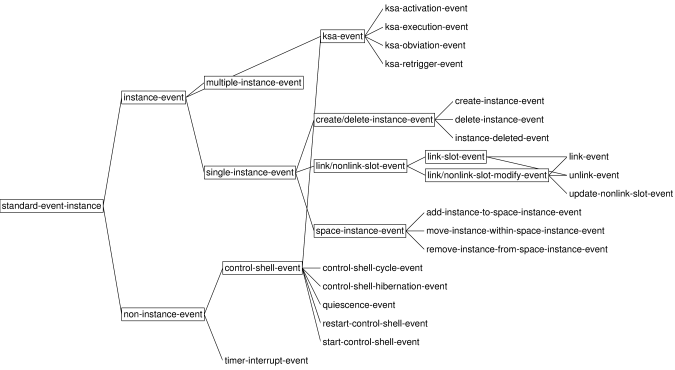
\includegraphics[scale=0.85]{agenda-shell-events}
\end{center}
\W\end{iftex}
%
Event classes shown within rectangles are abstract event classes that cannot
be signaled.  Nevertheless, abstract event classes are very convenient if we
wish to attach an event function to an entire subtree of event classes.  We
used abstract event classes to advantage earlier when we enabled display of
all control-shell events by evaluating:
%
\W\supp
\begin{example}
\textcolor{darkergray}{%
  gbbopen-user> (enable-event-printing '(control-shell-event :plus-subevents))
  nil
  gbbopen-user>}
\end{example}

Add the following form at the end of your \code{tutorial-example.lisp} file:
%
\W\supp
\begin{example}
  (add-event-function 'initializations 'start-control-shell-event
                      ;; Initializations should be done first!
                      :priority 100)
\end{example}
%
(We'll place the \textbf{add-event-function} form immediately after the
\code{initializations} function definition in our file, but this choice of
location is purely a code organizational style preference---the form could be
placed anywhere relative to the function definition.)

\subsection*{Step 3: Run the application}

\bfindex{start-control-shell}%
%
Start a fresh Common Lisp session, compile and load the
\code{tutorial-example.lisp} file directly from the editor buffer (using
\code{C-c C-k} in SLIME; \code{C-c C-b} in ELI) and start the Agenda Shell
again:
%
\W\supp
\begin{example}
\textcolor{darkergray}{%
  gbbopen-user> \textcolor{black}{(start-control-shell)}
  ;; Control shell 1 started
  ;; No executable KSAs remain, exiting control shell
  ;; Control shell 1 exited: 3 cycles completed
  ;; Run time: 0 seconds
  ;; Elapsed time: 0 seconds
  :quiescence
  gbbopen-user>}
\end{example}

Note that our developing application performs the same as it did in the last
exercise, but now our \code{initializations} event function is taking care of
all the details of starting up our application.  We no longer have to remember
to create the \code{known-world} space instance or to delete the blackboard
repository before running the application another time.

\subsection*{Step 4: Run it Again}

\bfindex{start-control-shell}%
%
Let's verify that we can re-run our application. Without doing anything else,
start the Agenda Shell again:
%
\W\supp
\begin{example}
\textcolor{darkergray}{%
  gbbopen-user> \textcolor{black}{(start-control-shell)}
  ;; Control shell 1 started
  ;; No executable KSAs remain, exiting control shell
  ;; Control shell 1 exited: 3 cycles completed
  ;; Run time: 0 seconds
  ;; Elapsed time: 0 seconds
  :quiescence
  gbbopen-user>}
\end{example}

As before, our \code{initializations} event function took care of all the
details of starting up our application.

\subsection*{Step 5: It's a new world$\ldots$}

\bfindexit{make-space-instance}%
%
GBBopen allows us to restrict the classes of unit instances that can be stored
on a space instance.  For example, we can limit the \code{known-world} to
\code{location} unit instances by specifying an \code{:allowed-unit-classes}
value to \code{make-space-instance}:
%
\W\supp
\begin{example}
\textcolor{darkergray}{%
  (defun initializations (event-name &key &allow-other-keys)
    (declare (ignore event-name))
    ;; Clean up any previous run:
    (delete-blackboard-repository)
    ;; Make a new known-world space instance:
    (make-space-instance 
     '(known-world)
     \textcolor{black}{:allowed-unit-classes '(location)}
     :dimensions '((x :ordered) (y :ordered))))}
\end{example}
%
Attempting to add any unit-instance that is not a \code{location} to
\code{known-world} will now generate an error.

It is often convenient to specify the dimensions of a space-instance relative
to those of one or more unit classes.  Edit the definition of
\code{initializations}, removing the \code{x} and \code{y} dimensions
specification:
%
\W\supp
\begin{example}
\textcolor{darkergray}{%
  (defun initializations (event-name &key &allow-other-keys)
    (declare (ignore event-name))
    ;; Clean up any previous run:
    (delete-blackboard-repository)
    ;; Make a new known-world space instance:
    (make-space-instance 
     '(known-world)
     :allowed-unit-classes '(location)
     :dimensions \textcolor{red}{'((x :ordered) (y :ordered))}))}
\end{example}
%
and replacing it with a call of \textbf{dimensions-of} to
obtain the dimensions associated with instances of the \code{location}
unit class:
%
\W\supp\notpretop
\begin{example}
\textcolor{darkergray}{%
  (defun initializations (event-name &key &allow-other-keys)
    (declare (ignore event-name))
    ;; Clean up any previous run:
    (delete-blackboard-repository)
    ;; Make a new known-world space instance:
    (make-space-instance 
     '(known-world)
     :allowed-unit-classes '(location)
     :dimensions \textcolor{black}{(dimensions-of 'location)}))}
\end{example}

\subsection*{Step 6: Run the application again}

Compile and load the \code{tutorial-example.lisp} file directly from the
editor buffer (using \code{C-c C-k} in SLIME; \code{C-c C-b} in ELI) and start
the Agenda Shell again:
%
\W\supp
\begin{example}
\textcolor{darkergray}{%
  gbbopen-user> \textcolor{black}{(start-control-shell)}
  ;; Control shell 1 started
  ;; No executable KSAs remain, exiting control shell
  ;; Control shell 1 exited: 3 cycles completed
  ;; Run time: 0 seconds
  ;; Elapsed time: 0 seconds
  :quiescence
  gbbopen-user>}
\end{example}

\bfindexit{describe-space-instance}%
Verify the dimensionality of the \code{known-world} space instance by
evaluating:
%
\W\supp
\begin{example}
\textcolor{darkergray}{%
  gbbopen-user> \textcolor{black}{(describe-space-instance '(known-world))}
  Standard-space-instance #<standard-space-instance (known-world)>
    Allowed unit classes: t
    Dimensions:
      (x :ordered)
      (y :ordered)
  gbbopen-user>}
\end{example}

%% ========================================================================
%%  Define Another KS

\T\markright{}%
\T\pagestyle{plain}
\T\cleardoublepage
\W\xname{tutorial-another-ks}
\T\pagestyle{fancy}
\T\thispagestyle{fancybottom}
\T\renewcommand{\headrulewidth}{0pt}
\section{Add Another KS}
\label{sec:another-ks}%

The last exercise made it easy to initialize and run our application
repeatedly by simply starting the Agenda Shell.  We also specified the
dimensionality of our \code{known-world} space instance relative to the
dimensional specifications of the \code{location} unit class.  With these
niceties in place, its time to move beyond our initial \code{location} unit
instance.

\fndocrule

This exercise shows you how to:
\begin{tightitemize}
\item Add an additional dimension to a unit class
\item Define a KS that obtains its execution-context information from its
  triggering unit instance
\item Extend the random-walk application to do some walking
\item Explore the resulting random walk
\end{tightitemize}

\fndocrule

\subsection*{Prerequisites}

\begin{tightitemize}
\item The \code{tutorial-example.lisp} file as modified thus far:
\end{tightitemize}
%
\W\supp
\begin{example}
  (in-package :gbbopen-user)

  (define-unit-class location ()
    (x y)
    (:dimensional-values
      (x :point x)
      (y :point y))
    (:initial-space-instances (known-world)))

  (defmethod print-instance-slots ((location location) stream)
    (call-next-method)
    (when (and (slot-boundp location 'x)
               (slot-boundp location 'y))
      (format stream " (~s ~s)"
              (x-of location)
              (y-of location))))

  ;;; ====================================================================
  ;;;   Startup KS

  (defun startup-ks-function (ksa)
    (declare (ignore ksa))
    ;; Create an initial location unit instance at (0,0):
    (make-instance 'location :x 0 :y 0))

  (define-ks startup-ks
      :trigger-events ((start-control-shell-event))
      :execution-function 'startup-ks-function)

  ;;; ====================================================================
  ;;;   Initializations (run at Agenda Shell startup)

  (defun initializations (event-name &key &allow-other-keys)
    (declare (ignore event-name))
    ;; Clean up any previous run:
    (delete-blackboard-repository)
    ;; Make a new known-world space instance:
    (make-space-instance 
     '(known-world)
     :dimensions (dimensions-of 'location)))

  (add-event-function 'initializations 'start-control-shell-event
                      ;; Initializations should be done first!
                      :priority 100)
\end{example}

\begin{tightitemize}
\item The \code{:agenda-shell-user} module is loaded
\end{tightitemize}

\subsection*{Step 1: Add  another dimension}

It's time we introduce the notion of time to our application.  Edit the
\code{location} unit-class definition in \code{tutorial-example.lisp}, adding
a new slot, \code{time}, to the \code{location} unit class definition and a
corresponding \code{time} dimensional value:
%
\W\supp
\begin{example}
\textcolor{darkergray}{%
  (define-unit-class location ()
    (\textcolor{black}{time} 
     x y)
    (:dimensional-values
      \textcolor{black}{(time :point time)}
      (x :point x)
      (y :point y))
    (:initial-space-instances (known-world)))}
\end{example}

Recall that we specified that the dimensions of the \code{known-world} space
instance that is created by our \code{initializations} function relative to
the dimensions of the \code{location} unit class:
%
\W\supp
\begin{example}
\textcolor{darkergray}{%
  (make-space-instance 
      '(known-world)
      :dimensions (dimensions-of 'location)))}
\end{example}
%
Therefore, we don't need to modify our call to \code{make-space-instance} in
order to add \code{time} as a dimension of \code{known-world}.

Next, modify \code{startup-ks-function} in \code{tutorial-example.lisp} so
that it creates the initial \code{location} unit instance at time 0:
%
\W\supp
\begin{example}
\textcolor{darkergray}{%
  (defun startup-ks-function (ksa)
    (declare (ignore ksa))
    ;; Create an initial location unit instance at (0,0) \textcolor{black}{at time 0}:
    (make-instance 'location \textcolor{black}{:time 0} :x 0 :y 0))}
\end{example}

\subsection*{Step 2: A test of time}

Let's verify our work.  Compile and load the \code{tutorial-example.lisp} file
directly from the editor buffer (using \code{C-c C-k} in SLIME; \code{C-c C-b}
in ELI) and start the Agenda Shell:
%
\W\supp
\begin{example}
\textcolor{darkergray}{%
  gbbopen-user> \textcolor{black}{(start-control-shell)}
  ;; Control shell 1 started
  ;; No executable KSAs remain, exiting control shell
  ;; Control shell 1 exited: 3 cycles completed
  ;; Run time: 0 seconds
  ;; Elapsed time: 0 seconds
  :quiescence
  gbbopen-user>}
\end{example}

\bfindexit{describe-instance}%
\bfindexit{find-instance-by-name}%
Check that the initial \code{location} unit instance is at \code{time} zero:
%
\W\supp
\begin{example}
\textcolor{darkergray}{%
  gbbopen-user> \textcolor{black}{(describe-instance (find-instance-by-name 1 'location))}
  Location #<location 1 (0 0)>
    Instance name: 1
    Space instances: ((known-world))
    Dimensional values:
      time:  0
      x:  40
      y:  60
    Non-link slots:
      time:  0
      x:  40
      y : 60
    Link slots: None
  gbbopen-user>}
\end{example}

\subsection*{Step 3: Define another KS}

Define a KS called \code{random-walk-ks} that:
%
\begin{tightitemize}
\item Is triggered when a \code{location} unit instance is created
\item Has a constant KSA rating of 100
\item Has an execution function called \code{random-walk-ks-function}, which:
\begin{tightitemize}
\item Checks if we've already walked for 75 locations and prints a message if
  we have. 
\item Otherwise:
\begin{tightitemize}
\item Determines a random location for which the x and y values are within 10
  of the x and y values of the triggering unit instance (that is, the
  \code{location} instance whose creation triggered the \code{random-walk-ks}
  KS)
\item If both of the x and y values for the new random location are between
  -50 and 50, creates a \code{location} unit instance at the random location;
  otherwise, prints a message indicating that we've walked off the world
\end{tightitemize}
\end{tightitemize}
\end{tightitemize}

\subsubsection*{Step 3a: Define a utility function}

Begin implementing the \code{random-walk-ks} by adding the following
utility function to the end of your \code{tutorial-example.lisp} file:
%
\W\supp
\begin{example}
  ;;; ====================================================================
  ;;;   Random-walk KS

  (defun add-linear-variance (value max-variance)
    ;;; Returns a new random value in the interval
    ;;; [(- value max-variance), (+ value max-variance)]
    (+ value (- (random (1+ (* max-variance 2))) max-variance)))
\end{example}
%
Then compile the definition (using \code{C-c C-c} in SLIME or \code{C-c
  C-x} in ELI) and evaluate the following test in the REPL:
%
\bfindex{printv}%
%
\W\supp\notpretop
\begin{example}
\textcolor{darkergray}{%
  gbbopen-user> \textcolor{black}{(dotimes (i 15) (printv (add-linear-variance 0 10)))}
  ;;  (add-linear-variance 0 10) => 8
  ;;  (add-linear-variance 0 10) => 9
  ;;  (add-linear-variance 0 10) => 4
  ;;  (add-linear-variance 0 10) => 3
  ;;  (add-linear-variance 0 10) => -4
  ;;  (add-linear-variance 0 10) => -10
  ;;  (add-linear-variance 0 10) => -1
  ;;  (add-linear-variance 0 10) => 0
  ;;  (add-linear-variance 0 10) => 4
  ;;  (add-linear-variance 0 10) => 5
  ;;  (add-linear-variance 0 10) => 8
  ;;  (add-linear-variance 0 10) => -5
  ;;  (add-linear-variance 0 10) => -3
  ;;  (add-linear-variance 0 10) => 7
  ;;  (add-linear-variance 0 10) => 6
  nil
  gbbopen-user>}
\end{example}

Because \code{add-linear-variance} is stochastic, your results will be
similar but not identical.  Note that we used GBBopen's \textbf{printv}
macro to display the result of each generated value.  \textbf{Printv} can
greatly assist debugging by printing forms and the results of evaluating
them.  \textbf{Printv} can be transparently wrapped around any form in a
complex function definition, as it evaluates and displays all the forms in
its body and returns the values resulting from evaluating the last form:
%
\W\supp
\begin{example}
\textcolor{darkergray}{%
  gbbopen-user>  (printv "Some multiple values" (values 1 2) "Some more" (values 3 4 5))
  ;; Some multiple values
  ;;  (values 1 2) => 1; 2
  ;; Some more
  ;;  (values 3 4 5) => 3; 4; 5
  4
  5
  6
  gbbopen-user>}
\end{example}

\subsubsection*{Step 3b: Define the \code{random-walk-ks} execution function}

Next add the following KS-execution function to the end of your
\code{tutorial-example.lisp} file:
%
\W\supp
\begin{example}
  (defun random-walk-ks-function (ksa)
    ;;; Move to the next (random) location in the world
    (let* ((trigger-instance (sole-trigger-instance-of ksa))
           ;; The new time is one greater than the stimulus's time:
           (time (1+ (time-of trigger-instance))))
      (cond
       ;; If the maximum time value (75) is reached, tell the user we've
       ;; walked too long:
       ((>= time 75) (format t "~2&Walked too long.~\%"))
       (t ;; The new location is +/- 10 of the stimulus's location:
        (let ((x (add-linear-variance (x-of trigger-instance) 10))
              (y (add-linear-variance (y-of trigger-instance) 10)))
          (cond
           ;; Check that the new location is within the known-world
           ;; boundaries.  If so, create the new location instance:
           ((and (<= -50 x 50) (<= -50 y 50))
            (make-instance 'location 
              :time time 
              :x x 
              :y y))
           ;; Otherwise, tell the user that we've walked too far away:
           (t (format t "~2\&Walked off the world: (~d, ~d).~\%" x y))))))))
\end{example}

\bfindex{sole-trigger-instance-of}%
%
Unlike the KS-execution functions that we have defined previously,
\code{random-walk-ks-function} does not ignore its \code{ksa} argument.
Instead, it calls \textbf{sole-trigger-instance-of} with the \code{ksa}
unit-instance argument in order to obtain the \code{location} unit instance
whose creation triggered the KSA.  This pattern of obtaining the unit instance
that triggered a KSA and then using that triggering unit instance as the
context for the KS execution is typical of many KSs. 

\subsubsection*{Step 3c: Add the \code{random-walk-ks} definition}

Finally, add this \code{define-ks} form to the end of your
\code{tutorial-example.lisp} file to complete the \code{random-walk-ks}
definition:
%
\bfindexit{define-ks}%
\codeindex{quiescence-event}%
\W\supp
\begin{example}
  (define-ks random-walk-ks
     :trigger-events ((create-instance-event location))
     :rating 100
     :execution-function 'random-walk-ks-function)
\end{example}

\subsection*{Step 4:  Run the application}

\bfindexit{start-control-shell}%
%
Compile and load the \code{random-walk-ks} forms, and then start the Agenda
Shell:
%
\W\supp
\begin{example}
\textcolor{darkergray}{%
  gbbopen-user> \textcolor{black}{(start-control-shell)}
  ;; Control shell 1 started

  Walked off the world: (23, 55).
  ;; No executable KSAs remain, exiting control shell
  ;; Control shell 1 exited: 64 cycles completed
  ;; Run time: 0.01 seconds
  ;; Elapsed time: 0 seconds
  :quiescence
  gbbopen-user>}
\end{example}

\bfindexit{:dsbb}%
It looks like something happened! (Again, because \code{add-linear-variance}
is stochastic, your results will be similar but not identical.)  Let's look at
the blackboard repository and see how many \code{location} unit instances were
created:
%
\W\supp
\begin{example}
\textcolor{darkergray}{%
  gbbopen-user> \textcolor{black}{:dsbb}

  Space Instance                Contents
  --------------                --------
  known-world                   61 instances (61 location)

  Unit Class                    Instances
  ----------                    ---------
  control-shell                         1 *
  ks                                    1 +
  ksa-queue                             2 +
  location                             61
  ordered-ksa-queue                     1 +
  standard-space-instance               1
                                ---------
                                       67 instances
  gbbopen-user>}
\end{example}

The 61 \code{location} instances makes sense.  Previously, it required 3
control-shell cycles to create the initial \code{location} unit instance (one
to execute the \code{initial-ks} KSA followed by two additional cycles of
quiescence before the Agenda Shell exits).  We now create one additional
\code{location} unit instance with every execution of \code{random-walk-ks},
so we always create 3 fewer \code{location} instances than the total
number of control-shell cycles.

\subsection*{Step 5:  Where have we been?}

\bfindexit{map-instances-of-class}%
%
It would be interesting to see where our random walk has taken us.  We could
use GBBopen's \textbf{map-instances-of-class} iterator to print each of the
\code{location} unit instances:
%
\W\supp
\begin{example}
\textcolor{darkergray}{%
  gbbopen-user> \textcolor{black}{(map-instances-of-class #'print 'location)}

  #<location 58 (5 31)> 
  #<location 13 (-7 10)> 
  #<location 26 (-40 35)> 
  #<location 39 (-4 3)> 
  #<location 52 (2 23)> 
  #<location 7 (3 17)> 
  #<location 20 (2 27)> 
  #<location 33 (-25 6)> 
  #<location 46 (-2 32)> 
       ...
  #<location 31 (-22 18)> 
  #<location 44 (-7 14)> 
  #<location 57 (2 41)> 
  #<location 12 (-15 15)> 
  #<location 25 (-32 38)> 
  #<location 38 (-10 -4)> 
  #<location 51 (-2 16)> 
  #<location 6 (10 27)> 
  #<location 19 (-1 17)> 
  #<location 32 (-25 12)> 
  #<location 45 (-7 23)> 
  nil
  gbbopen-user>}
\end{example}
%
Unfortunately, the order that unit instances are supplied to the \code{print}
function is not controllable.  Our walk would be much clearer if we printed
the \code{location}s in time order.

\bfindexit{map-sorted-instances-of-class}%
%
We might consider taking advantage of the instance names that GBBopen assigns
to unit instances.  We could do something like the following:
%
\W\supp
\begin{example}
\textcolor{darkergray}{%
  gbbopen-user> \textcolor{red}{(dotimes (i 76)
                  (let ((location (find-instance-by-name i 'location)))
                    (when location
                       (print location))))}

  #<location 1 (0 0)> 
  #<location 2 (10 4)> 
  #<location 3 (19 10)> 
  #<location 4 (14 9)> 
  #<location 5 (14 18)> 
  #<location 6 (10 27)> 
  #<location 7 (3 17)> 
  #<location 8 (-6 20)> 
  #<location 9 (4 15)> 
  #<location 10 (-5 14)> 
       ...
  #<location 50 (5 26)> 
  #<location 51 (-2 16)> 
  #<location 52 (2 23)> 
  #<location 53 (9 33)> 
  #<location 54 (7 43)> 
  #<location 55 (-2 36)> 
  #<location 56 (0 46)> 
  #<location 57 (2 41)> 
  #<location 58 (5 31)> 
  #<location 59 (13 39)> 
  #<location 60 (17 41)> 
  #<location 61 (21 50)> 
  nil
  gbbopen-user>}
\end{example}

This is a bad idea for several reasons.  First, we are looking up every
\code{location} unit instance by its instance name, which is less efficient
than operating on \code{location} instances directly.  While this isn't an
significant issue in expressions that we evaluate in the REPL to investigate
our application, we should seek to avoid such inefficiencies in application
code.  More importantly, however, the \code{location} instance name just
happens to mirror the sequencing that we really want to display---the
\code{time} value of the \code{location}s.  We should find a way to sequence
\code{location} printing that relies on the \code{time} values directly.

\bfindex{map-sorted-instances-of-class}%
%
GBBopen provides a variant of \textbf{map-instances-of-class}, called
\textbf{map-sorted-instances-of-class}, that sorts the unit instances based on
a comparison predicate and an optional \code{:key} accessor function that
suits our needs:
%
\W\supp
\begin{example}
\textcolor{darkergray}{%
  gbbopen-user> \textcolor{black}{(map-sorted-instances-of-class #'print 'location #'< 
                   :key #'time-of)}

  #<location 1 (0 0)> 
  #<location 2 (10 4)> 
  #<location 3 (19 10)> 
  #<location 4 (14 9)> 
  #<location 5 (14 18)> 
  #<location 6 (10 27)> 
  #<location 7 (3 17)> 
  #<location 8 (-6 20)> 
  #<location 9 (4 15)> 
  #<location 10 (-5 14)> 
       ...
  #<location 50 (5 26)> 
  #<location 51 (-2 16)> 
  #<location 52 (2 23)> 
  #<location 53 (9 33)> 
  #<location 54 (7 43)> 
  #<location 55 (-2 36)> 
  #<location 56 (0 46)> 
  #<location 57 (2 41)> 
  #<location 58 (5 31)> 
  #<location 59 (13 39)> 
  #<location 60 (17 41)> 
  #<location 61 (21 50)> 
  nil
  gbbopen-user>}
\end{example}

\bfindex{do-sorted-instances-of-class}%
%
Using \textbf{map-sorted-instances-of-class} involves a sorting operation, so
this approach still has some efficiency concerns for use in application code.
However, it suits our REPL-exploration needs just fine.  (There is a
\textbf{do-sorted-instances-of-class} macro, if an iterative style is
preferred over a mapper.)  We will explore a more efficient approach to
displaying the random walk in the next exercise.

\subsection*{Step 6:  Run the application a few more times}

\bfindexit{start-control-shell}%
%
If we run the application a few more times, we eventually encounter a case
where we create the allotted 75 \code{location} unit instances without walking
off the \code{known-world}:
%
\W\supp
\begin{example}
\textcolor{darkergray}{%
  gbbopen-user> \textcolor{black}{(start-control-shell)}
  ;; Control shell 1 started

  Walked too long.
  ;; No executable KSAs remain, exiting control shell
  ;; Control shell 1 exited: 78 cycles completed
  ;; Run time: 0.04 seconds
  ;; Elapsed time: 0 seconds
  :quiescence
  gbbopen-user>}
\end{example}

\bfindexit{map-sorted-instances-of-class}%
Here is one such random walk:
%
\W\supp
\begin{example}
\textcolor{darkergray}{%
  gbbopen-user> \textcolor{black}{(map-sorted-instances-of-class #'print 'location #'< 
                   :key #'time-of)}

  #<location 1 (0 0)> 
  #<location 2 (2 7)> 
  #<location 3 (-1 5)> 
  #<location 4 (-1 0)> 
  #<location 5 (3 -2)> 
  #<location 6 (13 -7)> 
  #<location 7 (8 -5)> 
  #<location 8 (1 2)> 
  #<location 9 (8 0)> 
  #<location 10 (5 8)> 
       ...
  #<location 70 (-13 -11)> 
  #<location 71 (-13 -6)> 
  #<location 72 (-9 -6)> 
  #<location 73 (1 -4)> 
  #<location 74 (-8 -11)> 
  #<location 75 (-13 -15)> 
  nil
  gbbopen-user>}
\end{example}

%% ========================================================================
%%  Making Connections

\T\markright{}%
\T\pagestyle{plain}
\T\cleardoublepage
\W\xname{tutorial-connections}
\T\pagestyle{fancy}
\T\thispagestyle{fancybottom}
\T\renewcommand{\headrulewidth}{0pt}
\section{Making Connections}
\label{sec:connections}%

%\begin{center}
%\textcolor{caution}{[Construction ahead...]}
%\end{center}

We finally did some walking in the last exercise and learned how to display
the \code{location}s in our walk from the REPL.  In this exercise, we learn
how to use GBBopen's link capabilities to represent relationships among unit
instances.  Links are an important aspect of almost every GBBopen application,
so it's time that we started taking advantage of them.

\fndocrule

This exercise shows you how to:
\begin{tightitemize}
\item Add link slots to a unit class
\item Use link slots to traverse and display the resulting random walk
\end{tightitemize}

\fndocrule

\subsection*{Prerequisites}

\begin{tightitemize}
\item The \code{tutorial-example.lisp} file as modified thus far:
\end{tightitemize}
%
\begin{example}
\W\supp
  (in-package :gbbopen-user)

  (define-unit-class location ()
    (time 
     x y)
    (:dimensional-values
      (time :point time)
      (x :point x)
      (y :point y))
    (:initial-space-instances (known-world)))

  (defmethod print-instance-slots ((location location) stream)
    (call-next-method)
    (when (and (slot-boundp location 'x)
               (slot-boundp location 'y))
      (format stream " (~s ~s)"
              (x-of location)
              (y-of location))))

  ;;; ====================================================================
  ;;;   Startup KS

  (defun startup-ks-function (ksa)
    (declare (ignore ksa))
    ;; Create an initial location unit instance at (0,0):
    (make-instance 'location :time 0 :x 0 :y 0))

  (define-ks startup-ks
      :trigger-events ((start-control-shell-event))
      :execution-function 'startup-ks-function)

  ;;; ====================================================================
  ;;;   Initializations (run at Agenda Shell startup)

  (defun initializations (event-name &key &allow-other-keys)
    (declare (ignore event-name))
    ;; Clean up any previous run:
    (delete-blackboard-repository)
    ;; Make a new known-world space instance:
    (make-space-instance 
     '(known-world)
     :dimensions (dimensions-of 'location)))

  (add-event-function 'initializations 'start-control-shell-event
                      ;; Initializations should be done first!
                      :priority 100)

  ;;; ====================================================================
  ;;;   Random-walk KS

  (defun add-linear-variance (value max-variance)
    ;;; Returns a new random value in the interval
    ;;; [(- value max-variance), (+ value max-variance)]
    (+ value (- (random (1+ (* max-variance 2))) max-variance)))

  (defun random-walk-ks-function (ksa)
    ;;; Move to the next (random) location in the world
    (let* ((trigger-instance (sole-trigger-instance-of ksa))
           ;; The new time is one greater than the stimulus's time:
           (time (1+ (time-of trigger-instance))))
      (cond
       ;; If the maximum time value (75) is reached, tell the user we've
       ;; walked too long:
       ((>= time 75) (format t "~2&Walked too long.~\%"))
       (t ;; The new location is +/- 10 of the stimulus's location:
        (let ((x (add-linear-variance (x-of trigger-instance) 10))
              (y (add-linear-variance (y-of trigger-instance) 10)))
          (cond
           ;; Check that the new location is within the known-world
           ;; boundaries.  If so, create the new location instance:
           ((and (<= -50 x 50) (<= -50 y 50))
            (make-instance 'location 
              :time time 
              :x x 
              :y y))
           ;; Otherwise, tell the user that we've walked too far away:
           (t (format t "~2&Walked off the world: (~d, ~d).~\%" x y))))))))

  (define-ks random-walk-ks
      :trigger-events ((create-instance-event location))
      :rating 100
      :execution-function 'random-walk-ks-function)
\end{example}

\begin{tightitemize}
\item The \code{:agenda-shell-user} module is loaded
\end{tightitemize}

\subsection*{Step 1: Add  a link}

In the last exercise, we used \textbf{map-sorted-instances-of-class} to
display the random walk.  Another way that we could represent the walk is by
connect each newly created \code{location} unit instance to the
\code{location} unit instance that preceded it in the walk.  We'll use
GBBopen's link capabilities to do this.

A \textit{link} is a bidirectional relationship between two unit instances
that is implemented by two pointers. From the perspective of a particular unit
instance, each link consists of an outgoing, or \textit{direct}, pointer to
another unit instance and an incoming, or \textit{inverse}, pointer that is
stored in unit instance pointed to by the direct pointer.  GBBopen
automatically maintains the bidirectional-link consistency of these pointers
when creating new links, deleting existing links, or deleting unit instances.
Links remove the possibility of ``one-sided'' relationships or ``dangling''
pointers to deleted unit instances.

Edit the \code{location} unit-class definition in your
\code{tutorial-example.lisp} file, adding two link slots, \code{next-location}
and \code{previous-location}, to the \code{location} unit class definition:
%
\W\supp
\begin{example}
\textcolor{darkergray}{%
  (define-unit-class location ()
    (time 
     x y
     \textcolor{black}{(next-location
      :link (location previous-location :singular t) 
      :singular t)
     (previous-location
      :link (location next-location :singular t)  
      :singular t)})
    (:dimensional-values
      (time :point time)
      (x :point x)
      (y :point y))
    (:initial-space-instances (known-world)))}
\end{example}

Each link-slot specification is a list whose first element is the name of the
link slot.  This is followed by the link slot option \code{:link} and a
concise specification of the inverse link slot associated with that link slot.
In this case, the \code{next-location}/\code{previous-location} link is
between instances of the same (\code{location}) unit class, but often links
are between instances of different unit classes. 

Links can be many-to-many, many-to-one, one-to-many, or one-to-one.  In this
case, the \code{next-location}/\code{previous-location} link is one-to-one,
which is specified by including the \code{:singular t} slot option in the
link-slot definition (and the corresponding \code{:singular t} specification
in the concise inverse-link-slot specification).  To help clarify the
specification of link slot arity, let's temporarily assume that we want a
\code{location} instance that can have many next locations, but only a single
previous location.  This link relation would be specified as follows:
%
\W\supp
\begin{example}
\textcolor{darkergray}{%
      ...
   \textcolor{blue}{(next-locations
    :link (location previous-location :singular t)))
   (previous-location
    :link (location next-locations)  
    :singular t)}
      ...}
\end{example}

We've followed the natural GBBopen convention of giving singular link
slots a singular name (such as \code{previous-location}) and link
slots that can contain multiple links a plural name (such as
\code{next-locations}).  Note that the \code{:singular} option is
associated with the \code{previous-location} link slot as both a slot
option in the \code{previous-location} link-slot definition and in the
concise inverse-link-slot specification for \code{previous-location}
in the \code{next-locations} link-slot definition.

\subsection*{Step 2: Break some links}

The concise inverse-link-slot specification supplied by the
\code{:link} slot option provides a ``double entry'' redundancy that
is useful when links are between instances of different unit classes,
as the link can be understood by viewing either class definition.  The
redundancy also helps GBBopen recognize inconsistencies in link
specifications.  The function \textbf{check-link-consistency} asks
GBBopen to validate that all link definitions are consistent.  Let's
try it on our current random-walk application.  Compile and load the
latest changes in your \code{tutorial-example.lisp} file (including
the new \code{next-location} and \code{previous-location} link slots).
Then check link consistency:
%
\W\supp
\begin{example}
\textcolor{darkergray}{%
  gbbopen-user> \textcolor{black}{(check-link-consistency)}
  ;; All link definitions are consistent.
  t
  gbbopen-user>}
\end{example}
%
GBBopen reports that all link definitions are consistent.

Suppose that we had forgotten to add the \code{previous-location} end
of the link in our \code{location} unit-class definition. Edit the
\code{location} unit-class definition in your
\code{tutorial-example.lisp} file, adding the line \code{\#+ignore}
immediately before the \code{previous-location} link-slot definition:
%
\W\supp
\begin{example}
\textcolor{darkergray}{%
  (define-unit-class location ()
    (time 
     x y
     (next-location
      :link (location previous-location :singular t) 
      :singular t)
      \textcolor{black}{\#+ignore}     
     (previous-location
      :link (location next-location :singular t)  
      :singular t))
    (:dimensional-values
      (time :point time)
      (x :point x)
      (y :point y))
    (:initial-space-instances (known-world)))}
\end{example}

The \code{\#+ignore} read-time conditionalization tells Common Lisp to
skip over the next form if \code{ignore} is not an element of the
feature list \code{*features*}.  By convention, \code{ignore} is never
added to \code{*features*}, so \code{\#+ignore} is a handy mechanism
for temporarily ``commenting out'' a single form.

Compile the now-defective definition (using \code{C-c C-c} in SLIME or
\code{C-c C-x} in ELI) and then recheck link consistency:
%
\W\supp
\begin{example}
\textcolor{darkergray}{%
  gbbopen-user> \textcolor{black}{(check-link-consistency)}
  Warning: The inverse of link slot next-location in unit class location 
           refers to link slot previous-location which is not present in 
           unit class location.
  nil
  gbbopen-user>}
\end{example}
%
As expected, GBBopen alerts us to the problem.

Remove the \code{\#+ignore} that we just added and comment out the
\code{:singular t} portion of the inverse link-slot specification in 
\code{next-location}:
%
\W\supp
\begin{example}
\textcolor{darkergray}{%
  (define-unit-class location ()
    (time 
     x y
     (next-location
      :link (location previous-location\textcolor{black}{) ;} :singular t) 
      :singular t)
      \textcolor{red}{#+ignore}     
     (previous-location
      :link (location next-location :singular t)  
      :singular t))
    (:dimensional-values
      (time :point time)
      (x :point x)
      (y :point y))
    (:initial-space-instances (known-world)))}
\end{example}
%
Compile the again-defective definition (using \code{C-c C-c} in SLIME or
\code{C-c C-x} in ELI) and then recheck link consistency:
%
\W\supp\notpretop
\begin{example}
\textcolor{darkergray}{%
  gbbopen-user> \textcolor{black}{(check-link-consistency)}
  Warning: Link slot next-location in unit class location incorrectly 
           declares its inverse link slot previous-location in unit 
           class location as not singular.
  nil
  gbbopen-user>}
\end{example}
%
Once again, GBBopen has alerted us to the problem.

Restore the \code{:singular t} portion of the inverse link-slot
specification in \code{next-location} that we just commented out:
%
\W\supp
\begin{example}
\textcolor{darkergray}{%
  (define-unit-class location ()
    (time 
     x y
     (next-location
      :link (location previous-location\textcolor{red}{) ;} :singular t) 
      :singular t)
     (previous-location
      :link (location next-location :singular t)  
      :singular t))
    (:dimensional-values
      (time :point time)
      (x :point x)
      (y :point y))
    (:initial-space-instances (known-world)))}
\end{example}
%
Then recompile and recheck link consistency:
%
\W\supp\notpretop
\begin{example}
\textcolor{darkergray}{%
  gbbopen-user> \textcolor{black}{(check-link-consistency)}
  ;; All link definitions are consistent.
  t
  gbbopen-user>}
\end{example}

\subsection*{Step 3: Create some links}

Let's use our newly defined \code{next-location}/\code{previous-location} link
to connect our \code{location} unit instances.  Edit the
\code{random-walk-ks-function} definition in your \code{tutorial-example.lisp}
file, adding the trigger instance as a new \code{:previous-location} argument
to \code{make-instance}:
%
\W\supp
\begin{example}
\textcolor{darkergray}{%
  (defun random-walk-ks-function (ksa)
    ;;; Move to the next (random) location in the world
    (let* ((trigger-instance (sole-trigger-instance-of ksa))
           ;; The new time is one greater than the stimulus's time:
           (time (1+ (time-of trigger-instance))))
      (cond
       ;; If the maximum time value (75) is reached, tell the user we've
       ;; walked too long:
       ((>= time 75) (format t "~2&Walked too long.~\%"))
       (t ;; The new location is +/- 10 of the stimulus's location:
        (let ((x (add-linear-variance (x-of trigger-instance) 10))
              (y (add-linear-variance (y-of trigger-instance) 10)))
          (cond
           ;; Check that the new location is within the known-world
           ;; boundaries.  If so, create the new location instance:
           ((and (<= -50 x 50) (<= -50 y 50))
            (make-instance 'location 
              :time time 
              :x x 
              :y y
              \textcolor{black}{:previous-location trigger-instance}))
           ;; Otherwise, tell the user that we've walked too far away:
           (t (format t "~2&Walked off the world: (~d, ~d).~\%" x y))))))))}
\end{example}

Compile the \code{random-walk-ks-function} (using \code{C-c C-c} in SLIME or
\code{C-c C-x} in ELI) and then run the application:
%
\W\supp
\begin{example}
\textcolor{darkergray}{%
  gbbopen-user> \textcolor{black}{(start-control-shell)}
  ;; Control shell 1 started

  Walked off the world: (55, 35).
  ;; No executable KSAs remain, exiting control shell
  ;; Control shell 1 exited: 66 cycles completed
  ;; Run time: 0.01 seconds
  ;; Elapsed time: 0 seconds
  :quiescence
  gbbopen-user>}
\end{example}

Let's describe a couple of \code{location} unit instances to check our work.
First, the initial \code{location} unit instance:
%
\W\supp
\begin{example}
\textcolor{darkergray}{%
  gbbopen-user> \textcolor{black}{(describe-instance (find-instance-by-name 1 'location))}
  Location #<location 1 (0 0)>
    Instance name: 1
    Space instances: ((known-world))
    Dimensional values:
      time:  0
      x:  40
      y:  60
    Non-link slots:
      time:  0
      x:  40
      y:  60
    Link slots:
      next-location:  #<location 2 (-10 10)>
      previous-location:  nil
  gbbopen-user>}
\end{example}
%
Note that the \code{next-location} link slot points to the next
\code{location} unit instance in our random walk.  Let's describe that
unit instance:
%
\W\supp\notpretop
\begin{example}
\textcolor{darkergray}{%
  gbbopen-user> \textcolor{black}{(describe-instance (find-instance-by-name 2 'location))}
  Location #<location 2 (-10 10)>
    Instance name: 2
    Space instances: ((known-world))
    Dimensional values:
      time:  1
      x:  -10
      y:  10
    Non-link slots:
      time:  1
      x:  -10
      y:  10
    Link slots:
      next-location:  #<location 3 (-6 19)>
      previous-location:  #<location 1 (0 0)>
  gbbopen-user>}
\end{example}
%
The \code{next-location} link slot in \code{location} \code{2} points to the
third \code{location} unit instance in our random walk and its
\code{previous-location} link slot points back to the initial \code{location}
unit instance.

We can now follow the links to display the random walk:
%
\W\supp
\begin{example}
\textcolor{darkergray}{%
  gbbopen-user> \textcolor{black}{(loop with location = (find-instance-by-name 1 'location) 
                  do (print location)
                  while (setf location (next-location-of location)))}

  #<location 1 (0 0)> 
  #<location 2 (-10 10)> 
  #<location 3 (-6 19)> 
  #<location 4 (0 14)> 
  #<location 5 (-1 14)> 
  #<location 6 (8 10)> 
  #<location 7 (17 3)> 
  #<location 8 (7 -6)> 
  #<location 9 (10 4)> 
  #<location 10 (5 -5)> 
       ...
  #<location 60 (29 17)> 
  #<location 61 (31 21)> 
  #<location 62 (40 23)> 
  #<location 63 (45 28)> 
  nil
  gbbopen-user>}
\end{example}

\subsection*{Step 4: Define a ``print walk'' KS}

\bfindexit{define-ks}%
\codeindex{:stop}%
\codeindex{quiescence-event}%
\bfindexit{find-instance-by-name}%
Let's add a new KS, \code{print-walk-ks}, that displays the random walk once
it is completed. Add the following KS to the end of your
\code{tutorial-example.lisp} file:
%
\W\supp
\begin{example}
  ;;; ====================================================================
  ;;;   Print-walk KS

  (defun print-walk-ks-function (ksa)
    ;;; Starting with the initial location instance, print the instance 
    ;;; name and location of the walk
    (declare (ignore ksa))
    (format t "~2\&The random walk:~\%")
    (let ((instance (find-instance-by-name 1 'location)))
      (while instance
        (format t "~s (~s ~s)~\%"
                (instance-name-of instance)
                (x-of instance)
                (y-of instance))
        (setf instance (next-location-of instance))))
    ;; Tell the Agenda Shell to exit:
    ':stop)

  (define-ks print-walk-ks
    :trigger-events ((quiescence-event))
    :rating 100
    :execution-function 'print-walk-ks-function)
\end{example}
%
The \code{print-walk-ks} is triggered by a \code{quiescence-event}.  Recall
that the Agenda Shell signals that quiescence has occurred when no
executable KSAs are available to be executed and then it continues for an
additional KS-execution cycle in case any executable KSAs resulted from the
quiescence event.  So, \code{print-walk-ks} will be triggered once no
\code{random-walk-ks} KSAs are triggered by newly created \code{location} unit
instances.

The \code{print-walk-ks-function} follows the
\code{next-location}/\code{previous-location} link to display the walk.  More
importantly, the function returns the keyword symbol \code{:stop}.  The Agenda
Shell checks the value returned by a KS execution function for this special
indicator and, if it is returned, the control shell is exited.  If we did not
return \code{:stop}, the \code{print-walk-ks} KS would be triggered and
activated on the first \code{quiescence-event}, the KSA would execute, then
the Agenda Shell would detect another quiescence condition, signal a new
\code{quiescence-event}, and our application would print the random walk over
and over again.

Let's compile our latest changes and then run our application with the new
\code{print-walk-ks} KS in place:
%
\W\supp
\begin{example}
\textcolor{darkergray}{%
  gbbopen-user> \textcolor{black}{(start-control-shell)}
  ;; Control shell 1 started

  Walked off the world: (54, 15).

  The random walk:
  1 (0 0)
  2 (-6 9)
  3 (-14 8)
  4 (-5 6)
  5 (-13 5)
  6 (-11 13)
  7 (-11 4)
  8 (-17 8)
  9 (-21 15)
  10 (-12 14)
       ...
  35 (40 28)
  36 (50 22)
  37 (49 12)
  38 (47 10)
  ;; Explicit :stop issued by KS print-walk-ks
  ;; Control shell 1 exited: 41 cycles completed
  ;; Run time: 0.01 seconds
  ;; Elapsed time: 0 seconds
  :stop
  gbbopen-user>}
\end{example}

%% ========================================================================
%%  Creating an Application

\T\markright{}%
\T\pagestyle{plain}
\T\cleardoublepage
\W\xname{tutorial-application}
\T\pagestyle{fancy}
\T\thispagestyle{fancybottom}
\T\renewcommand{\headrulewidth}{0pt}
\section{Creating a GBBopen Application}
\label{sec:application}%

GBBopen's \xreflink{Mini Module system}{sec:mini-module} provides facilities
that make it easy to define and use your own GBBopen applications.

\fndocrule

This exercise shows you how to:
\begin{tightitemize}
\item Structure an application using the \xreflink{Mini Module
    system}{sec:mini-module}
\item Define a REPL command for your application
\item Compile and load your application using your REPL command
\item Create and use an application-specific package
\item Add an ``autorun'' action
\end{tightitemize}

\fndocrule

\subsection*{Prerequisites}

\begin{tightitemize}
\item The \code{tutorial-example.lisp} file as modified thus far:
%
\W\supp\notpretop
\begin{example}
  (in-package :gbbopen-user)

  (define-unit-class location ()
    (time 
     x y
     (next-location
      :link (location previous-location :singular t) 
      :singular t)
     (previous-location
      :link (location next-location :singular t)  
      :singular t))
    (:dimensional-values
      (time :point time)
      (x :point x)
      (y :point y))
    (:initial-space-instances (known-world)))

  (defmethod print-instance-slots ((location location) stream)
    (call-next-method)
    (when (and (slot-boundp location 'x)
               (slot-boundp location 'y))
      (format stream " (~s ~s)"
              (x-of location)
              (y-of location))))

  ;;; ====================================================================
  ;;;   Startup KS

  (defun startup-ks-function (ksa)
    (declare (ignore ksa))
    ;; Create an initial location unit instance at (0,0):
    (make-instance 'location :time 0 :x 0 :y 0))

  (define-ks startup-ks
      :trigger-events ((start-control-shell-event))
      :execution-function 'startup-ks-function)

  ;;; ====================================================================
  ;;;   Initializations (run at Agenda Shell startup)

  (defun initializations (event-name &key &allow-other-keys)
    (declare (ignore event-name))
    ;; Clean up any previous run:
    (delete-blackboard-repository)
    ;; Make a new known-world space instance:
    (make-space-instance 
     '(known-world)
     :dimensions (dimensions-of 'location)))

  (add-event-function 'initializations 'start-control-shell-event
                      ;; Initializations should be done first!
                      :priority 100)

  ;;; ====================================================================
  ;;;   Random-walk KS

  (defun add-linear-variance (value max-variance)
    ;;; Returns a new random value in the interval
    ;;; [(- value max-variance), (+ value max-variance)]
    (+ value (- (random (1+ (* max-variance 2))) max-variance)))

  (defun random-walk-ks-function (ksa)
    ;;; Move to the next (random) location in the world
    (let* ((trigger-instance (sole-trigger-instance-of ksa))
           ;; The new time is one greater than the stimulus's time:
           (time (1+ (time-of trigger-instance))))
      (cond
       ;; If the maximum time value (75) is reached, tell the user we've
       ;; walked too long:
       ((>= time 75) (format t "~2&Walked too long.~\%"))
       (t ;; The new location is +/- 10 of the stimulus's location:
        (let ((x (add-linear-variance (x-of trigger-instance) 10))
              (y (add-linear-variance (y-of trigger-instance) 10)))
          (cond
           ;; Check that the new location is within the known-world
           ;; boundaries.  If so, create the new location instance:
           ((and (<= -50 x 50) (<= -50 y 50))
            (make-instance 'location 
              :time time 
              :x x 
              :y y
              :previous-location trigger-instance))
           ;; Otherwise, tell the user that we've walked too far away:
           (t (format t "~2\&Walked off the world: (~d, ~d).~\%" x y))))))))

  (define-ks random-walk-ks
      :trigger-events ((create-instance-event location))
      :rating 100
      :execution-function 'random-walk-ks-function)

  ;;; ====================================================================
  ;;;   Print-walk KS

  (defun print-walk-ks-function (ksa)
    ;;; Starting with the initial location instance, print the instance
    ;;; name and location of the walk
    (declare (ignore ksa))
    (format t "~2\&The random walk:~\%")
    (let ((instance (find-instance-by-name 1 'location)))
      (while instance
        (format t "~s (~s ~s)~\%"
                (instance-name-of instance)
                (x-of instance)
                (y-of instance))
        (setf instance (next-location-of instance))))
    ;; Tell the Agenda Shell to exit:
    ':stop)

  (define-ks print-walk-ks
    :trigger-events ((quiescence-event))
    :rating 100
    :execution-function 'print-walk-ks-function)
\end{example}

\item The GBBopen environment setup using
  \code{\var{<install-dir>\/}/initiate.lisp} as described in Steps 1 and 2
  of the \reflink{Enhancing Your Development Environment
    exercise}{sec:environment}
\end{tightitemize}

\subsection*{Step 1: Create your personal \code{gbbopen-modules} directory}

Create a directory named \code{gbbopen-modules} in your \reflink{``homedir''
  directory}{ref:your-homedir}.  For example:
%
\W\supp
\begin{example}
\textcolor{darkergray}{%
  [~]\$ \textcolor{black}{mkdir gbbopen-modules}
  [~]\$}
\end{example}
%
This is a special directory that is read by used by GBBopen to find
applications when GBBopen is started using
\code{\var{<install-dir>\/}/initiate.lisp}, as described in Steps 1 and 2
of the \reflink{Enhancing Your Development Environment
  exercise}{sec:environment}.

\subsection*{Step 2: Create a module-definition file for the random-walk application}

Recall that you created a directory to hold the random-walk application in
Step 1 of \reflink{Working Within a File exercise}{sec:file}.  I used these
shell commands to create my directories:
%
\W\supp
\begin{example}
\textcolor{darkergray}{%
  [~]\$ mkdir tutorial
  [~]\$ cd tutorial
  [~/tutorial]\$ mkdir source
  [~/tutorial]\$}
\end{example}
%
Then you created the \code{tutorial-example.lisp} file in this \code{source}
subdirectory. We said that we would explain why we created the \code{source}
directory in a later exercise.  Well, later has arrived.

Each GBBopen application is packaged in a directory that contains:
\begin{tightitemize}
\item a \code{modules.lisp} file that contains module definitions (loaded
  after the personal \code{gbbopen-init.lisp} file if
  there is one in the user's ``homedir'')
\item a directory named \code{source} containing all the source files for the
  module or application
\item an optional \code{commands.lisp} file that specifies REPL commands
  for the module (loaded after the personal \code{gbbopen-commands.lisp} file
  if there is one in the user's ``homedir'')
\end{tightitemize}
%
You already have the \code{source} directory and the
\code{tutorial-example.lisp} source file.  Next, we create the
\code{modules.lisp} file for the application.  (We will create a
\code{commands.lisp} file for the random-walk application in Step 5.)

Use your Common Lisp editor to create a new file named \code{modules.lisp} in
the \code{tutorial} directory (just as you created the
\code{tutorial-example.lisp} file in Step 2 of \reflink{Working Within a File
  exercise}{sec:file}.  Note that this file is \textit{not\/} in the
\code{source} subdirectory, but in the \code{tutorial} directory that contains
the \code{source} subdirectory.

Type the following two forms into the new \code{modules.lisp}
file:
%
\W\supp
\begin{example}
  (in-package :common-lisp-user)

  (define-module :tutorial
    (:requires :agenda-shell-user)
    (:files "tutorial-example"))
\end{example}
%
and then save the file.

Recall that the \code{in-package} form specifies the Common Lisp package that
is made current when the file is compiled or loaded.  A \code{modules.lisp}
file should always specify the \code{:mini-module-user} package as the first
form in the file.

The second form defines our application module, which we will name
\code{:tutorial}.  The \code{:requires} subform specifies that the
\code{:agenda-shell-user} module must be compiled (if necessary) and then
loaded before our \code{:tutorial} module.  The \code{:files} subform
specified the files that comprise the module. In our case, there is one file:
\code{tutorial-example.lisp}.  We leave off the \code{.lisp} file extension,
as the \xreflink{Mini Module system}{sec:mini-module} will add the appropriate
source or compiled file extension for us.

\subsection*{Step 3: Add the random-walk application to your personal
  \code{gbbopen-modules} directory}

The \code{gbbopen-modules} directory in your ``homedir'' is expected to
consist of directories each containing an individual GBBopen application.  We
could place the random-walk application directly in the \code{gbbopen-modules}
directory by moving the \code{tutorial} directory there.  However, it is
generally more convenient to use a symbolic link to point to the actual
application directory.  For example, an application can be provided to a
number of users by creating a symbolic link to the application directory in
each user's \code{gbbopen-modules} directory.

Unless you are running Windows, add the random-walk application to your
\code{gbbopen-applications} by creating a symbolic link.  For example:
%
\W\supp
\begin{example}
\textcolor{darkergray}{%
  [~]\$ \textcolor{black}{cd ~/gbbopen-modules/}
  [~]\$ \textcolor{black}{ln -s ~/tutorial .}
  [~]\$}
\end{example}

\subsubsection*{Windows users}

Instead of creating a symbolic link, GBBopen also supports a special ``pseudo
symbolic-link'' file that can be used with Windows.  This is simply a text
file of type \code{.sym} that contains the target directory path as the sole
line in the file.  For example, you could create the file \code{tutorial.sym}
in your \code{gbbopen-modules} directory with:
%
\W\supp
\begin{example}
  C:\bkslash{}tutorial\bkslash
\end{example}
\T\vskip -12pt
%
as the sole line in the file.

\subsection*{Step 4: Try the \code{:tutorial} module definition}

Let's try out our module definition.  Exit Common Lisp and start a fresh
Common Lisp session.  If you have set up your environment according to the
\reflink{Enhancing Your Development Environment exercise}{sec:environment},
the following files should be loaded:
%
\W\supp
\begin{example}
\textcolor{darkergray}{%
     ...
  ;; Loading \var{<homedir>\/}/shared-init.lisp
  ;;   Loading \var{<install-dir>\/}/initiate.lisp
  ;;     Loading \var{<install-dir>\/}/extended-repl.lisp
  ;;     Loading \var{<install-dir>\/}/commands.lisp
  ;;     Loading \var{<install-dir>\/}/gbbopen-modules-directory.lisp
  ;; Loading module command definitions from \var{<homedir>\/}/gbbopen-modules/...
  cl-user>}
\end{example}

Note that some basic GBBopen initialization files have been loaded for us (but
no command definitions yet) and that GBBopen itself (or even the Mini Module
system) are not loaded by \code{\var{<install-dir>\/}/initiate.lisp}.

Now, instead of loading the \code{:agenda-shell-user} module, let's load only
the \code{:mini-module-user} module:
%
\W\supp
\begin{example}
\textcolor{darkergray}{%
  cl-user> \textcolor{black}{:mini-module-user}
  ;; Loading \var{<install-dir>\/}/startup.lisp
     ...
  ;;     Loading \var{<install-dir>\/}/\var{<platform-dir>\/}/mini-module/mini-module-user.fasl
  ;;   Loading \var{<install-dir>\/}/modules.lisp
  ;; Loading module definitions from \var{<homedir>\/}/gbbopen-modules/...
  ;;     Loading \var{<homedir>\/}/tutorial/modules.lisp
  mini-module-user>}
\end{example}
%
Note that when the Mini Module system was loaded as part of loading the
\code{:mini-module-user} module, the module definitions for our personal
GBBopen modules were loaded automatically.  (In this case, the
\code{\var{<homedir>\/}/tutorial/modules.lisp} file.)  

Now that we have defined our \code{:tutorial} module, we can use the
\textbf{compile-module} REPL command, \code{:cm}, to compile (if needed) and
load it:
%
\W\supp
\begin{example}
\textcolor{darkergray}{%
  mini-module-user> \textcolor{black}{:cm :tutorial}
  ;;   Loading \var{<install-dir>\/}/\var{<platform-dir>\/}/tools/portable-threads.fasl
     ...
  ;;   Loading .../gbbopen/control-shells/agenda-shell-user.fasl

  Error: Directory \var{<homedir>\/}/tutorial/\var{<platform-dir>\/}/ 
         in module :tutorial doesn't exist.

  Restart actions (select using :c n):
    0: Create this directory.
    1: Create this directory and any future missing directories.
  mini-module-user>>}
\end{example}
%
The \code{:requires} in our \code{:tutorial} module definition causes the
\code{:agenda-shell-user} module (and its required modules) to be loaded for
us.  Then the Mini Module system stops with a continuable error, telling us
that the directory to hold the compiled application files does not exist.  The
compiled files are put in a Common Lisp and platform-specific subdirectory,
\code{<\var{platform-dir>\/}}, in our \code{tutorial} directory that mirrors
the \code{source} directory.  This organization makes it easy to use the
application with a number of Common Lisp implementations and on a file system
shared with a number of different hosts and operating systems.

We could have avoided this continuable error by providing the
\code{:create-dirs} option to the \code{:cm} command:
%
\W\supp
\begin{example}
\textcolor{darkergray}{%
  mini-module-user> :cm :tutorial :create-dirs}
\end{example}
%
to allow the Mini Module system to create the \code{<\var{platform-dir>\/}}
subdirectory automatically for us.  Since we did not do this, we can still
continue from the error:
%
\W\supp\notpretop
\begin{example}
\textcolor{darkergray}{%
  Restart actions (select using :c n):
    0: Create this directory.
    1: Create this directory and any future missing directories.
  mini-module-user>> \textcolor{black}{:c 0}
  ;; Compiling file \var{<homedir>\/}/tutorial/source/tutorial-example.lisp
  ;; Loading \var{<homedir>\/}/tutorial/\var{<platform-dir>\/}/tutorial-example.fasl
  mini-module-user>}
\end{example}

At this point, we've compiled and loaded our \code{:tutorial} application
module.

\subsection*{Step 5: Create a command-definition file for the random-walk
  application}

It is convenient to define a REPL command to compile and load you application
(and any required GBBopen modules).  

Use your Common Lisp editor to create a new file named \code{commands.lisp} in
the \code{tutorial} directory. Type the following two forms into the new
\code{commands.lisp} file:
%
\W\supp
\begin{example}
(in-package :common-lisp-user)

(define-repl-command :tutorial (\&rest options)
  "Compile and load the Random-Walk Tutorial Application Module"
  (startup-module :tutorial options :gbbopen-user))
\end{example}
%
and then save the file.  A \code{commands.lisp} file should always specify the
\code{:common-lisp-user} package as the first form in the file.

The \textbf{define-repl-command} form adds a REPL command, named
\code{:tutorial}, to the set of handy REPL commands.  The
\textbf{startup-module} call does all the work associated with executing the
command.  The first argument to \textbf{startup-module} specifies that the
\code{:tutorial} module will be compiled (if necessary) and then loaded by the
\xreflink{Mini Module system}{sec:mini-module} when the \code:{tutorial}
command is issued.  The second, \code{options}, argument passes any options
given with the command to a \textbf{compile-module} call that is performed by
\textbf{startup-module}.  The third argument, \code{:gbbopen-user} is optional
and specifies that the REPL's current package should be changed to \code{:gbbopen-user} after the \code{:tutorial} module is loaded. 

\subsection*{Step 6: Try the \code{:tutorial} command}

Let's try our command definition.  Exit Common Lisp and start a fresh
Common Lisp session.  If you have set up your environment according to the
\reflink{Enhancing Your Development Environment exercise}{sec:environment},
the following files should be loaded:
%
\W\supp
\begin{example}
\textcolor{darkergray}{%
     ...
  ;; Loading \var{<homedir>\/}/shared-init.lisp
  ;;   Loading \var{<install-dir>\/}/initiate.lisp
  ;;     Loading \var{<install-dir>\/}/extended-repl.lisp
  ;;     Loading \var{<install-dir>\/}/commands.lisp
  ;;     Loading \var{<install-dir>\/}/gbbopen-modules-directory.lisp
  ;; Loading module command definitions from \var{<homedir>\/}/gbbopen-modules/...
  ;      Loading \var{<homedir>}/gbbopen-modules/tutorial/commands.lisp
  cl-user>}
\end{example}
%
Note that the \code{commands.lisp} file from the \code{tutorial} directory has
been loaded by \code{\var{<install-dir>\/}/initiate.lisp}.

Now, we can compile and load the \code{:tutorial} module by simply issuing the
\code{:tutorial} REPL command:
%
\W\supp
\begin{example}
\textcolor{darkergray}{%
  cl-user> \textcolor{black}{:tutorial}
  ;; Loading \var{<install-dir>\/}/startup.lisp
     ...
  ;; Loading \var{<homedir>\/}/tutorial/\var{<platform-dir>\/}/tutorial-example.fasl
  gbbopen-user>}
\end{example}
%
With the command definition in place, we are able to compile and load our
random-walk application by issuing a single command, \code{:tutorial}.

Note a potential continuable error due to a missing
\code{\var{<platform-dir>\/}} subdirectory can always be avoided by providing
the \code{:create-dirs} option to the \code{:tutorial} command:
%
\W\supp
\begin{example}
\textcolor{darkergray}{%
  gbbopen-user> :tutorial :create-dirs}
\end{example}
%
to allow the Mini Module system to create the \code{\var{<platform-dir>\/}}
subdirectory automatically for us.  However, since we created
\code{\var{<platform-dir>\/}} in Step 4, we did not need to specify the
\code{:create-dirs} option again in this step.

\subsection*{Step 7: Create missing subdirectories automatically}

\bfindex{*automatically-create-missing-directories*} 
%
If you prefer, you can specify that the Mini Module system should always
create missing \code{\var{<platform-dir>\/}} directories and subdirectories
instead of signaling an continuable error if one is missing (and
\code{:create-dirs} was not specified).  This behavior is controlled by the
value of the symbol \textbf{*automatically-create-missing-directories*}, which
is in the \code{:common-lisp-user} package and is set to \nil{} by default.
If you wish, add the following form to your \code{shared-init.lisp} file (in
your ``homedir'' directory):
%
\W\supp
\begin{example}
  (defparameter *automatically-create-missing-directories* 't)
\end{example}

I actually prefer to have the Mini Module system generate the continuable
error if it has to create a \code{\var{<platform-dir>\/}} directory and I
didn't specify \code{:create-dirs}, so I leave
\textbf{*automatically-create-missing-directories*} set to the default \nil{}
value.

\subsection*{Step 8: Create and use an application-specific package}

We have been developing our random-walk application in GBBopen's
\code{:gbbopen-user} package.  The \code{:gbbopen-user} package is convenient,
and we could continue using it.  However, if we develop multiple GBBopen
applications in the \code{:gbbopen-user} package and load several of them at
the same time, symbol-name clashes could occur.

To eliminate this possibility, we can create our own package for the
random-walk application.  First, let's determine what packages are being used by GBBopen's \code{:gbbopen-user} package.  Evaluate the following:
%
\W\supp
\begin{example}
\textcolor{darkergray}{%
  gbbopen-user> \textcolor{black}{(package-use-list :gbbopen-user)}
  (#<package PORTABLE-THREADS> #<package AGENDA-SHELL>
   #<package MINI-MODULE> #<package COMMON-LISP> #<package CLOS>
   #<package GBBOPEN-TOOLS> #<package GBBOPEN>)
  gbbopen-user>}
\end{example}
%
The \code{CLOS} package does not have a standard name in Common Lisp, so the
package that you see listed may be named differently (such as \code{ACLMOP} or
\code{SB-PCL}).  GBBopen provides the \code{:clos} nickname when necessary, so
that you can reference the ``\code{CLOS}'' package using \code{:clos} on any
supported Common Lisp implementation.

\subsubsection*{Change \code{tutorial-example.lisp}}
%
We want our new \code{:tutorial} package to use the same packages that the
\code{:agenda-shell-user} package used. Edit your \code{tutorial-example.lisp}
file and replace the \code{:gbbopen-user} package specification:
%
\W\supp
\begin{example}
  \textcolor{red}{(in-package :gbbopen-user)}
\end{example}
%
with the following:
%
\W\supp\notpretop
\begin{example}
  (eval-when (:compile-toplevel :load-toplevel :execute)
    (unless (find-package :tutorial)
      (defpackage :tutorial
        (:use :common-lisp :clos :mini-module :gbbopen-tools :gbbopen 
              :portable-threads :agenda-shell))))

  (in-package :tutorial)
\end{example}
%
and save the file.

Note the use of \code{eval-when} in the first form above.  Normally, top-level
forms in a file are not evaluated at compile time.  In this case, however, we
want to define the \code{:tutorial} package when needed, whether the file is
being compiled or loaded.  The \code{eval-when} special operator with the
three situations (\code{:compile-toplevel}, \code{:load-toplevel}, and \code{
  :execute}) provides this behavior to the forms that it contains.  Such
\code{eval-when} forms are a standard Common Lisp idiom for compile-time and
load-time evaluation.

\subsubsection*{An application feature}
%
In my applications, I also add a feature to Common Lisp's \code{*features*}
list to indicate that the application has been fully loaded.  To do this, add
the following at the end of your \code{tutorial-example.lisp} file:
%
\W\supp
\begin{example}
  (pushnew :tutorial *features*)
\end{example}
%
and save the file.

\subsubsection*{Change \code{commands.lisp}}
%
Next, edit your \code{commands.lisp} file and delete the \code{:gbbopen-user}
package-name argument to \textbf{startup-module}:
%
\W\supp
\begin{example}
\textcolor{darkergray}{%
  (define-repl-command :tutorial (\&rest options)
    "Compile and load the Random-Walk Tutorial Application Module"
    (startup-module :tutorial options \textcolor{red}{:gbbopen-user}))}
\end{example}
%
and add the package-name \code{:tutorial} in its place:
%
\W\supp\notpretop
\begin{example}
\textcolor{darkergray}{%
  (define-repl-command :tutorial (\&rest options)
    "Compile and load the Random-Walk Tutorial Application Module"
    (startup-module :tutorial options \textcolor{black}{:tutorial}))}
\end{example}
%
Save the file.

\subsubsection*{Change \code{modules.lisp}}

\bfindexit{describe-module}%
%
Finally, we no longer need the \code{:gbbopen-user} package that is created by
requiring the \code{:agenda-shell-user} module.  Let's take a closer look at the \code{:tutorial} module that we defined:
%
\W\supp
\begin{example}
\textcolor{darkergray}{%
  gbbopen-user> \textcolor{black}{(describe-module :tutorial)}
  Module :tutorial (loaded)
    Requires: (:agenda-shell-user)
    Fully expanded requires: (:mini-module :mini-module-user :portable-threads
                              :gbbopen-tools :gbbopen-core :polling-functions
                              :queue :agenda-shell :os-interface :gbbopen-user
                              :agenda-shell-user)
    Source directory: \var{<homedir>\/}/tutorial/source/
    Compiled directory: \var{<homedir>\/}/\var{<platform-dir>\/}/
    Forces recompile date: None
    Files: Mar 24 06:02 tutorial-example
  gbbopen-user>}
\end{example}
%
Although we only specified that the \code{:agenda-shell-user} module was
required, our \code{:tutorial} module implicitly requires a number of packages
that are required by the \code{:agenda-shell-user} module and its implicitly
required packages.  These are shown as the ``Fully expanded requires'' value.

If we look at the details of the \code{:agenda-shell-user} module we see:
%
\W\supp
\begin{example}
\textcolor{darkergray}{%
  gbbopen-user> \textcolor{black}{(describe-module :agenda-shell-user)}
  Module :agenda-shell-user (loaded)
    Requires: (:agenda-shell :gbbopen-user)
    Fully expanded requires: (:mini-module :mini-module-user :portable-threads
                              :gbbopen-tools :gbbopen-core :polling-functions
                              :queue :agenda-shell :os-interface :gbbopen-user)
    Source directory: \var{<install-dir>\/}/source/gbbopen/control-shells/
    Compiled directory: \var{<install-dir>\/}/\var{<platform-dir>\/}/gbbopen/control-shells/
    Forces recompile date: None
    Files: Mar 23 12:27 agenda-shell-user 
  gbbopen-user>}
\end{example}
%
Note that the \code{:agenda-shell-user} module requires two modules:
\code{:agenda-shell} and \code{:gbbopen-user}. We can eliminate the loading of
the \code{:gbbopen-user} module by editing our \code{modules.lisp} file and
delete \code{:agenda-shell-user} in the \code{:requires} option in our
\code{:tutorial} module definition:
%
\W\supp\notpretop
\begin{example}
\textcolor{darkergray}{%
  (in-package :common-lisp-user)

  (define-module :tutorial
    (:requires \textcolor{red}{:agenda-shell-user})
    (:files "tutorial-example"))}
\end{example}
%
and replace it with \code{:agenda-shell}:
%
\W\supp\notpretop
\begin{example}
\textcolor{darkergray}{%
  (in-package :common-lisp-user)

  (define-module :tutorial
    (:requires \textcolor{black}{:agenda-shell})
    (:files "tutorial-example"))}
\end{example}
%
Save the file.

\subsection*{Step 9: Verify your changes}

Let's make sure that everything is still working.  Exit Common Lisp and start
a fresh Common Lisp session.  Next enter the
\code{:tutorial} REPL command:
%
\W\supp
\begin{example}
\textcolor{darkergray}{%
  cl-user> \textcolor{black}{:tutorial}
  ;; Loading \var{<install-dir>\/}/startup.lisp
     ...
  ;; Loading \var{<homedir>\/}/tutorial/\var{<platform-dir>\/}/tutorial-example.fasl
  tutorial>}
\end{example}
%
Note that we are now in our newly defined \code{:tutorial} package.  We should
still be able to run the random-walk application:
%
\W\supp\notpretop
\begin{example}
\textcolor{darkergray}{%
  tutorial> \textcolor{black}{(start-control-shell)}
  ;; Control shell 1 started

  Walked off the world:  (56, 38).

  The random walk:
  1 (0 0)
  2 (-1 -1)
  3 (-8 -10)
  4 (0 -2)
  5 (-5 2)
  6 (3 11)
  7 (8 5)
  8 (12 2)
  9 (3 12)
  10 (10 4)
       ...
  55 (50 40)
  56 (42 47)
  57 (47 41)
  ;; Explicit :stop issued by KS print-walk-ks
  ;; Control shell 1 exited: 60 cycles completed
  ;; Run time: 0.01 seconds
  ;; Elapsed time: 0 seconds
  :stop
  gbbopen-user>}
\end{example}

\subsubsection*{Installation-wide sharing}
%
\index{shared-gbbopen-modules@\code{shared-gbbopen-modules}, installation-wide application sharing}%

GBBopen also has an \code{\var{<install-directory>\/}/shared-gbbopen-modules}
directory.  As with our personal \code{gbbopen-modules} directory, this
\code{shared-gbbopen-modules} directory is assumed to contain symbolic links
(or ``pseudo-symbolic-link'' files on Windows) to individual GBBopen module
directory trees.

This is the recommended mechanism for installation-wide managing and sharing
of modules and applications, and if we wanted to share our random-walk
application to everyone using our GBBopen installation, we could create our
symbolic link (or ``pseudo-symbolic-link'' file) in the
\code{shared-gbbopen-modules} directory.

\subsection*{Step 10: Add an ``autorun'' action}

Suppose we want the random-walk application to run automatically when it is
loaded.  You could simply add:
% 
\W\supp
\begin{example}
\textcolor{darkergray}{% 
  (start-control-shell)}
\end{example}
%
as a top-level form at the end of your \code{tutorial-example.lisp} file.  The
problem with this is that sometimes you may want to compile and load the
application without running it.  

GBBopen's Mini Module system supports a convention that makes it easy to
conditionalize load-time action execution via the value of
\textbf{*autorun-modules*}.  Normally, \code{*autorun-modules*} will be
true, but it can be set to \nil{} when a module is loaded with the
\code{:noautorun} option.

Add the following at the end of your \code{tutorial-example.lisp}
file:
% 
\W\supp
\begin{example}
  (when *autorun-modules* 
    (format t "~\{~\&~s~\%~\}" (multiple-value-list (start-control-shell))))
\end{example}
%
and save the file.  We could have simply called \textbf{start-control-shell}
when \code{*autorun-modules*} is true, but then we would not be able to see
what values are returned by the Agenda Shell.  The \code{format} form above
prints each returned value on a separate output line.

By convention, the ``autorun'' form is placed at the very end of the file,
immediately after the form to add \code{:tutorial} to Common Lisp's
\code{*features*}.  This is so that the \code{:tutorial} feature will be
present during the ``autorun'' execution and thereafter---even if an error
occurs when executing the ``autorun'' form.

\subsection*{Step 11: Try it out}

Enter the \code{:tutorial} REPL command; the modified
\code{tutorial-example.lisp} file should compile and load, followed by a
random walk:
%
\W\supp
\begin{example}
\textcolor{darkergray}{%
  tutorial> \textcolor{black}{:tutorial}
  ;; Compiling \var{<homedir>\/}/tutorial/source/tutorial-example.lisp
  ;; Loading \var{<homedir>\/}/tutorial/\var{<platform-dir>\/}/tutorial-example.fasl
  ;; Control shell 1 started

  Walked off the world: (11, -51).

  The random walk:
  1 (0 0)
  2 (6 7)
  3 (6 3)
  4 (3 -4)
  5 (10 -13)
     ...
  21 (-5 -46)
  22 (-9 -39)
  23 (1 -33)
  24 (8 -41)
  ;; Explicit :stop issued by KS print-walk-ks
  ;; Control shell 1 exited: 27 cycles completed
  ;; Run time: 0.01 seconds
  ;; Elapsed time: 0 seconds
  :stop
  tutorial>}
\end{example}

Let's try it again:
%
\W\supp
\begin{example}
\textcolor{darkergray}{%
  tutorial> \textcolor{black}{:tutorial}
  tutorial>}
\end{example}
%
This time, nothing happened.  Why?

Since no source files were modified, the Mini Module system knows that the
latest compiled files for the \code{:tutorial} module and its required modules
have all been loaded.  So, because the \code{tutorial-example} file is not
loaded, its ``autorun'' conditional form is not evaluated.

We can tell the Mini Module system to always reload the
\code{tutorial-example} file by editing our \code{modules.lisp} file and
adding the \code{:reload} file option to the \code{:tutorial} module
definition:
%
\W\supp
\begin{example}
\textcolor{darkergray}{%
  (define-module :tutorial
    (:requires :agenda-shell)
    (:files \textcolor{black}{(}"tutorial-example" \textcolor{black}{:reload})))}
\end{example}
%
Note that once a file has one or more options, the file name and its options
are enclosed in parentheses.

Save the modified \code{modules.lisp} file. Now, if you try the
\code{:tutorial} command, the \code{tutorial-example} file will always be
loaded and its ``autorun'' form evaluated:
%
\W\supp
\begin{example}
\textcolor{darkergray}{%
  tutorial> \textcolor{black}{:tutorial}
  ;; Loading \var{<homedir>\/}/tutorial/modules.lisp
  ;; Loading \var{<homedir>\/}/tutorial/\var{<platform-dir>\/}/tutorial-example.fasl
  ;; Control shell 1 started
     ...
  tutorial>}
\end{example}
%
The Mini Module system noticed our updated \code{modules.lisp} file and loaded
it, redefining the \code{:tutorial} module definition, and then followed our
\code{:reload} specification.

Let's try the \code{:tutorial} command one more time, just to be certain that
\code{:reload} is happening when no files have been updated:
%
\W\supp
\begin{example}
\textcolor{darkergray}{%
  tutorial> \textcolor{black}{:tutorial}
  ;; Loading \var{<homedir>\/}/tutorial/\var{<platform-dir>\/}/tutorial-example.fasl
  ;; Control shell 1 started
     ...
  tutorial>}
\end{example}

\subsubsection*{Mini Module propagation}

The Mini Module's \textbf{compile-module} function also accepts a
\code{:reload} option, so we might be tempted to simply add that option when
we specify our \code{:tutorial} command:
%
\W\supp
\begin{example}
\textcolor{darkergray}{%
  tutorial> :tutorial :reload
  ;;   Loading \var{<install-dir>\/}/\var{<platform-dir>\/}/mini-module/mini-module.fasl
  ;;     Loading \var{<install-dir>\/}/\var{<platform-dir>\/}/mini-module/mini-module-user.fasl

     ...
  ;; Control shell 1 started
     ...
  tutorial>}
\end{example}
%
however, this would also reload all the files of very module required by the
\code{:tutorial} module, as the \textbf{startup-module} function that we used
in defining our \code{:tutorial} REPL command always adds a \code{:propagate}
option to the options that we provide to the command.  We could override
(cancel) this propagation behavior by adding the \code{:nopropagate} option
when we specify our \code{:tutorial} command:
%
\W\supp\notpretop
\begin{example}
\textcolor{darkergray}{%
  tutorial> :tutorial :reload :nopropagate
  ;; Loading \var{<homedir>\/}/tutorial/\var{<platform-dir>\/}/tutorial-example.fasl
  ;; Control shell 1 started
     ...
  tutorial>}
\end{example}
%
which would eliminate reloading of all but the files in the \code{:tutorial}
module.  Since we only have one file (at the moment) specified in our
\code{:tutorial} module definition, this behavior is equivalent, but less
convenient, than specifying the \code{:reload} file option to our
\code{tutorial-example} file in the module definition.  If we had a number of
files, however, we would probably only want the last one reloaded every time.

\subsubsection*{Mini Module memories}

The Mini Module system also remembers the last module (and any provided
options, such as \code{:create-dirs}) that was specified to a \code{:cm}
(textbf{compile-module}) or \code{:lm} (\textbf{load-module}) command.  The
\textbf{startup-module} function that we used in defining our \code{:tutorial}
REPL command performs an implicit \code{:cm} command for us, so we could have
alternatively typed the \code{:cm} REPL command rather than \code{:tutorial}
once we have issued the first \code{:tutorial} REPL command:
%
\W\supp
\begin{example}
\textcolor{darkergray}{%
  tutorial> \textcolor{black}{:cm}
  ;; :cm :tutorial :propagate
  ;; Loading \var{<homedir>\/}/tutorial/\var{<platform-dir>\/}/tutorial-example.fasl
  ;; Control shell 1 started
     ...
  tutorial>}
\end{example}
%
Just the thing for lazy typists like me!  Note that the \code{:cm} command
echos the full (implicitly completed) command with the remembered module name
and any remembered options.

\subsection*{Step 12: Add a second source file}

Reloading the entire \code{tutorial-application} file in order to evaluate our
``autorun'' form is still a bit heavy handed.  There are two ways to improve
this situation, and both involve placing the ``autorun'' form in a separate
file.  Use your Common Lisp editor to create a new file named
\code{autorun.lisp} in the \code{source} subdirectory of the \code{tutorial}
directory. Type (or copy) the following two forms into the new
\code{autorun.lisp} file:
%
\W\supp
\begin{example}
  (in-package :tutorial)

  (when *autorun-modules*
    (format t "~\{~\&~s~\%~\}" (multiple-value-list (start-control-shell))))
\end{example}
%
and save the file.  

Next, edit the \code{tutorial-example.lisp} file and remove the ``autorun''
form from the end of the file:
% 
\W\supp
\begin{example}
\textcolor{red}{% 
  (when *autorun-modules* 
    (format t "~\{~\&~s~\%~\}" (multiple-value-list (start-control-shell))))}
\end{example}
%
Save the file. 

We could define a second random-walk application module, say
\code{:run-tutorial}, in our \code{modules.lisp} file that contains the new
\code{autorun.lisp} file and requires our current \code{:tutorial} module.
This definition would look like:
%
\W\supp
\begin{example}
\textcolor{darkergray}{%
  (define-module :run-tutorial
    (:requires :tutorial
    (:files ("autorun" :reload))))}
\end{example}
%
However, we can avoid creating a new module by simply adding the
\code{autorun} file to our current \code{:tutorial} module definition.  

Edit the \code{modules.lisp} file in the \code{tutorial} directory and remove
the \code{:reload} file option from the \code{:tutorial-example} file
specification:
%
\W\supp
\begin{example}
\textcolor{darkergray}{%
  (define-module :tutorial
    (:requires :agenda-shell)
    (:files \textcolor{red}{(}"tutorial-example" \textcolor{red}{:reload)}))}
\end{example}
%
and then add a new line for the \code{autorun} file with the \code{:reload}
file option:
%
\W\supp\notpretop
\begin{example}
\textcolor{darkergray}{%
  (define-module :tutorial
    (:requires :agenda-shell)
    (:files "tutorial-example"
            \textcolor{black}{("autorun" :reload)}))}
\end{example}
%
and save the file.

\subsection*{Step 13: One last check}

Let's double-check that everything is working:
%
\W\supp
\begin{example}
\textcolor{darkergray}{%
  tutorial> \textcolor{black}{:cm}
  ;; :cm :tutorial :propagate
  ;; Loading \var{<homedir>\/}/tutorial/modules.lisp
  ;; Compiling \var{<homedir>\/}/tutorial/source/tutorial-example.lisp
  ;; Loading \var{<homedir>\/}/tutorial/\var{<platform-dir>\/}/tutorial-example.fasl
  ;; Compiling \var{<homedir>\/}/tutorial/source/autorun.lisp
  ;; Loading \var{<homedir>\/}/tutorial/\var{<platform-dir>\/}/autorun.fasl
  ;; Control shell 1 started
     ...
  tutorial>}
\end{example}
%
The modified files are compiled and loaded and the Agenda Shell is invoked.

Let's try it one last time, just to be sure that the application runs when no
files have been modified:
%
\W\supp
\begin{example}
\textcolor{darkergray}{%
  tutorial> \textcolor{black}{:cm}
  ;; :cm :tutorial :propagate
  ;; Loading \var{<homedir>\/}/tutorial/\var{<platform-dir>\/}/autorun.fasl
  ;; Control shell 1 started
     ...
  tutorial>}
\end{example}

Congratulations!  It's time to move to the next exercise.

%% ========================================================================
%%  Multiple Walkers

\T\markright{}%
\T\pagestyle{plain}
\T\cleardoublepage
\W\xname{tutorial-multiple-walkers}
\T\pagestyle{fancy}
\T\thispagestyle{fancybottom}
\T\renewcommand{\headrulewidth}{0pt}
\section{Multiple Walkers}
\label{sec:multiple-walkers}%

\T\medskip
\T\fndocrule\\
\T\begin{center}
\textcolor{darkergray}{\textsf{\textbf{Coming later $\ldots$\\~\\ 
 Please continue with the next exercise.}}}
\T\end{center}
\T\fndocrule

%% ========================================================================
%%  A Dimensional Detour

\T\markright{}%
\T\pagestyle{plain}
\T\cleardoublepage
\W\xname{tutorial-dimensional-detour}
\T\pagestyle{fancy}
\T\thispagestyle{fancybottom}
\T\renewcommand{\headrulewidth}{0pt}
\section{A Dimensional Detour}
\label{sec:detour}%

%\begin{center}
%\textcolor{caution}{[Construction ahead...]}
%\end{center}

\T\medskip
\T\fndocrule\\
\T\begin{center}
\textcolor{darkergray}{\textsf{\textbf{Coming later, exploration of unbound
 dimensional values, intersection of unit instance, space instance, and retrieval
 dimensionality, $\ldots$\\~\\ 
 Please continue with the next exercise.}}}
\T\end{center}
\T\fndocrule

%\subsection*{Step 1: Unbound dimensional values}

%% ========================================================================
%%  More to come...

\T\markright{}%
\T\pagestyle{plain}
\T\cleardoublepage
\W\xname{tutorial-more-to-come}
\T\pagestyle{fancy}
\T\thispagestyle{fancybottom}
\T\renewcommand{\headrulewidth}{0pt}

\W\section{More to come\ldots}
\T\section{More to come$\ldots$}
\T\medskip
\T\fndocrule\\
\T\begin{center}
\textcolor{darkergray}{\textsf{\textbf{Additional exercises will be 
      added soon.}}}
\T\end{center}
\T\fndocrule

%% ========================================================================
%%  The Completed Application

\T\markright{}%
\T\pagestyle{plain}
\T\cleardoublepage
\W\xname{tutorial-completed-application}
\T\pagestyle{fancy}
\T\thispagestyle{fancybottom}
\T\renewcommand{\headrulewidth}{0pt}
\section{The Completed Application}
\label{sec:completed}%

The complete, finished code for the random walk application is in the
\code{tutorial.lisp} file in the \code{source/gbbopen/examples/}
directory in the GBBopen distribution and at
\xsitelink{\code{http://gbbopen.org/svn/GBBopen/trunk/source/gbbopen/examples/tutorial.lisp}}{http://gbbopen.org/svn/GBBopen/trunk/source/gbbopen/examples/tutorial.lisp}.

%% ========================================================================
%%  Index

\renewcommand{\printindex}{%
  \htmlonly{\HlxSection{-5}{}*{\indexname}\label{hlxindex}}%
  \texorhtml{%% -*- Mode:TeX; Fonts:(hl12fb) -*-
%% *-* File: /usr/local/gbbopen/doc-source/tutorial.tex *-*
%% *-* Last-Edit: Mon Mar 24 11:00:36 2008; Edited-By: cork *-*
%% *-* Machine: cyclone.local *-*

%% Copyright (C) 2005-2008, Dan Corkill <corkill@GBBopen.org>
%% Part of the GBBopen Project (see LICENSE for license information).
%%
%% ========================================================================
%%  The LaTeX and hyperlatex code used in producing GBBopen documentation
%%  is placed under and covered by the GBBopen software license that 
%%  accompanies each GBBopen distribution and is also available at
%%  http://GBBopen.org/downloads/LICENSE. 
%% ========================================================================
%%
%%  Note: To keep both LaTeX and hyperlatex happy with indexing, index
%%        commands must be positioned with care (including the use of
%%        % after all entries).  Follow the placement used here to
%%        minimize the creation of anchors by hyperlatex.  Indexes
%%        should only be placed at locations where an inserted &nbsp; 
%%        anchor does not visibly affect the html layout.
%%
%%        \indexit doesn't play well with @\xxx{} formating, so use
%%        the basic \index{...|itidx} rather than \indexit shorthand.
        
\documentclass[10pt,twoside,english,pdftex]{article} 
\usepackage{hyperlatex}
\usepackage{color}
\usepackage{makeidx}
\T\usepackage{atbeginend}
%\T\usepackage{palatino}
\T\usepackage{newcent}
% Use smaller TT font throughout
\W\begin{iftex}
  \makeatletter
  \DeclareRobustCommand\smallttfamily
  {\not@math@alphabet\ttfamily\mathtt
    \fontfamily\ttdefault\small\selectfont}
  \makeatother
\W\end{iftex}
\T\usepackage{fancyhdr}
\W\usepackage{frames}
%% Req'd for pdflatex -- note use epstopdf to convert eps figures;
%%                       ps2pdf won't create correct bounding boxes
\T\newif\ifpdf\ifx\pdfoutput\undefined\pdffalse\else\pdfoutput=1\pdftrue\fi
\T\newcommand{\pdfgraphics}{\ifpdf\DeclareGraphicsExtensions{.pdf,.jpg}\else\fi}
\T\usepackage{graphicx}

\newcommand{\docname}{Tutorial}

%% -*- Mode:TeX; Fonts:(hl12fb) -*-
%% *-* File: /home/gbbopen/current/doc-source/test-common.tex *-*
%% *-* Last-Edit: Thu Dec 28 06:25:02 2006; Edited-By: cork *-*
%% *-* Machine: ruby.corkills.org *-*

%% Copyright (C) 2003-2006, Dan Corkill <corkill@GBBopen.org>
%% Part of the GBBopen Project (see LICENSE for license information).
%%
%% ========================================================================
%%  The LaTeX and hyperlatex code used in producing GBBopen documentation
%%  is placed under and covered by  the GBBopen software license that 
%%  accompanies each GBBopen distribution and is also available at
%%  http://GBBopen.org/downloads/LICENSE. 
%% ========================================================================

\newcommand{\noargs}{$<$no arguments$>$}
\T\newcommand{\bkslash}{$\backslash$}
\W\newcommand{\bkslash}{\backslash}
\T\newcommand{\vbar}{$|$}
\W\newcommand{\vbar}{|}
\T\newcommand{\superstar}{\raisebox{2pt}{*}}
\W\newcommand{\superstar}{*}
\T\newcommand{\superplus}{\raisebox{4pt}{+}}
\W\newcommand{\superplus}{\xml{sup}+\xml{/sup}}
\definecolor{rulegray}{gray}{.75}
\definecolor{darkergray}{gray}{.55}
\definecolor{caution}{rgb}{.8,.6,.0}

%% ----------------------------------------------------------------------------
%%   Margins

\T\headsep 26pt
\T\footskip 36pt
\T\topmargin -40pt
\T\oddsidemargin 0pt
\T\evensidemargin 0pt
\T\textwidth 470pt
\T\textheight 630pt

%% ----------------------------------------------------------------------------
%%   Headings/Footings

\W\begin{iftex}
\fancyhf{} % clear all
\fancyhead[er,ol]{\textcolor{darkergray}{\rightmark}}
\fancyfoot[er,ol]{\textcolor{darkergray}{\runningtitle}
                \\\textcolor{darkergray}{\nouppercase{\leftmark}}}
\fancyfoot[el,or]{~\\\thepage}

\makeatletter

%% from fancyhdr
\def\ps@fancy{%
\@ifundefined{@chapapp}{\let\@chapapp\chaptername}{}%for amsbook
%
% Define \MakeUppercase for old LaTeXen.
% Note: we used \def rather than \let, so that \let\uppercase\relax (from
% the version 1 documentation) will still work.
%
\@ifundefined{MakeUppercase}{\def\MakeUppercase{\uppercase}}{}%
\@ifundefined{chapter}{\def\sectionmark##1{\markboth
{\ifnum \c@secnumdepth>\z@
 \thesection\hskip 1em\relax \fi ##1}{}}%
\def\subsectionmark##1{\markboth {\ifnum \c@secnumdepth >\@ne
 \thesubsection\hskip 1em\relax \fi ##1}{}}}%
{\def\chaptermark##1{\markboth {\MakeUppercase{\ifnum \c@secnumdepth>\m@ne
 \@chapapp\ \thechapter. \ \fi ##1}}{}}%
\def\sectionmark##1{\markboth{\ifnum \c@secnumdepth >\z@
 \thesection. \ \fi ##1}{}}}%
\ps@@fancy
\gdef\ps@fancy{\@fancyplainfalse\ps@@fancy}%
\ifdim\headwidth<0sp
    \global\advance\headwidth123456789sp\global\advance\headwidth\textwidth
\fi}
\def\ps@fancyplain{\ps@fancy \let\ps@plain\ps@plain@fancy}
\def\ps@plain@fancy{\@fancyplaintrue\ps@@fancy}
\let\ps@@empty\ps@empty

%% mod of \headrule from fancyhdr.sty (to make rule gray):
\def\headrule{{\if@fancyplain\let\headrulewidth\plainheadrulewidth\fi
    \vskip-0.8\baselineskip % tighten rule to \rightmark
    \textcolor{rulegray}{\hrule\@height\headrulewidth\@width\headwidth 
    \vskip-\headrulewidth}}}

%% mod of \ps@@fancy from fancyhdr.sty:
\def\ps@fancybottom{%
\def\@mkboth{\protect\markboth}%
\def\@oddhead{}%
\def\@oddfoot{\@fancyfoot\fancy@Oolf\f@ncyolf\f@ncyocf\f@ncyorf\fancy@Oorf}%
\def\@evenhead{}%
\def\@evenfoot{\@fancyfoot\fancy@Oelf\f@ncyelf\f@ncyecf\f@ncyerf\fancy@Oerf}%
}
\makeatother
\W\end{iftex}

\T\begin{ifhtml}
\newcommand\entities{\textbf{\large Entities}}
\T\end{ifhtml}

%% ----------------------------------------------------------------------------
%%  LaTeX Modifications

\W\begin{iftex}
\makeatletter

% article.cls
\renewcommand\@idxitem{\par\hangindent 30\p@}
\renewcommand\subitem{\@idxitem \hspace*{10\p@}}
\renewcommand\subsubitem{\@idxitem \hspace*{20\p@}}
% ppar
\newcommand{\ppar}[1]{\paragraph{#1}~\\[0.5\baselineskip]%
  \T\addcontentsline{toc}{subsubsection}{{#1}}
}
% Tighten up example environment (uses atbeginend.sty):
\AfterBegin{example}{\vspace*{-0.8\baselineskip}}

% fndocsec
\newcommand{\fndocsec}{\@startsection{subparagraph}{5}{\z@}%
                          {1.25ex \@plus1ex \@minus.1ex}%
                          {-1em}%
                          {\normalfont\large\sffamily\bfseries}}
% from article.cls - Increase TOC font for sections and subsections
\renewcommand*\l@section[2]{%
  \ifnum \c@tocdepth >\z@
    \addpenalty\@secpenalty
    \addvspace{1.0em \@plus\p@}%
    \setlength\@tempdima{2.0em}%
    \begingroup
      \parindent \z@ \rightskip \@pnumwidth
      \parfillskip -\@pnumwidth
      \leavevmode \bfseries
      \advance\leftskip\@tempdima
      \hskip -\leftskip
      {\large #1}\nobreak\hfil \nobreak\hb@xt@\@pnumwidth{\hss\large #2}\par
    \endgroup
    \addvspace{.5em \@plus\p@}%
  \fi}
\renewcommand*\l@subsection[2]{%
  \ifnum \c@tocdepth >\z@
    \addpenalty\@secpenalty
    \addvspace{0.4em \@plus\p@}%
    \setlength\@tempdima{2.3em}%
    \begingroup
      \parindent \z@ \rightskip \@pnumwidth
      \parfillskip -\@pnumwidth
      \leavevmode \bfseries
      \advance\leftskip\@tempdima
      \hskip -\leftskip
      #1\nobreak\hfil \nobreak\hb@xt@\@pnumwidth{\hss #2}\par
    \endgroup
    \addvspace{.2em \@plus\p@}%
  \fi}
% from article.cls - Decrease TOC leftmargin for subsubsections
\renewcommand*\l@subsubsection{\@dottedtocline{3}{3.3em}{2.3em}}

\makeatother
\W\end{iftex}

%% ----------------------------------------------------------------------------
%%  HyperLaTeX Modifications

\T\begin{ifhtml}

  %% No easy CSS hook for this (we don't want to mess up the navbar
  %% alignment):
  \xmlattributes{td}{valign="baseline"}

  \newcommand{\textrm}[1]{\xml{span 
    style="font-family: serif; font-style: normal"}{#1}\xml{/span}}
  \newcommand{\textsf}[1]{\xml{span 
    style="font-family: sans-serif; font-style: normal"}{#1}\xml{/span}}

  %% This should be the URL for the icons used in the navigation panels
  %% must end with a slash, unless you leave it empty
  %% (empty means the icons are in the same directory as the HTML file)
  \renewcommand{\HlxIcons}{}
  \renewcommand{\HlxStyleSheet}{}

  \renewcommand{\HlxMeta}{\xml{link rel="SHORTCUT ICON" href="favicon.ico"}}

  %% Add `GoTo Top' to Panel
  \renewcommand{\HlxPanelFields}{\xml*{td bgcolor="##99ccff"}%
    \GoToTopTarget%
    \HlxImage{GoTo Top}{top.png}%
    \xml{/a}%
    \xml*{/td}}

  \newcommand{\HlxAddressDatetime}{}

  %% Add logo to Navigation Panel
  \renewcommand{\HlxFramesNavigation}{%
    \HlxTocName
    \htmlpanel{0}%
    \HlxSection{-5}{}*{\xml{img align="left" src="GBBopen-logo-sm.png"}%
      \xml{br clear="both"}%
      {\large \navigationname}}%
    \xml{base target="main"}%
    \htmlmenu[0]{1}
    \renewcommand{\HlxAddressDatetime}{,\xml{nobr}~\today{}\xml{/nobr}
      \xml{nobr}\hhmm~\timezone\xml{/nobr}}
    \renewcommand{\bottommatter}{}}

\renewcommand{\HlxBottomMatter}{%
  \HlxBlk\htmlrule\EmptyP{\HlxAddress}%
  {\xml{address}\HlxAddress%
  \EmptyP{\HlxAddressDatetime}{\HlxAddressDatetime}{}%
  \HlxBlk\xml{/address}\\}{}}

\T\end{ifhtml}

% Things to skip/fake in HyperLaTeX
\W\newcommand{\vspace}[1]{}
\W\newcommand{\bigskip}{\\}
\W\newcommand{\medskip}{\\}
\W\newcommand{\smallskip}{\\}
\W\newcommand{\vfill}{\\}
\W\newcommand{\hfill}{\xml{p align="right"}}
\W\newcommand{\normalbaselines}{}
\W\newcommand{\^}{\xmlent{##94}}
%\W\NotSpecial{\do\^}

%% ----------------------------------------------------------------------------
%%  Special link & index commands
%%
%%  Note that \entlink and index commands can insert a space in hyperlatex
%%  format

% The following doesn't work in LaTeX example environments, due to 
% kerning/hyphenation:
%\T\newcommand{\entlink}[1]{\hyperref[ent:#1]{#1}}
% This doesn't get there either, but shows the problem with already
% kerned hyphen in the example environment:
%\T\newcommand{\entlink}[1]{\bgroup\let\-\@@hyph\typeout{ent:#1}#1\egroup}
\newcommand{\entlink}[1]{\link{#1}{ent:#1}}
% Special non-example \entlink for LaTeX:
\T\newcommand{\entlinknoex}[1]{\hyperref[ent:#1]{#1}}
\W\newcommand{\entlinknoex}[1]{\entlink{#1}}
%
\newcommand{\bfindex}[1]{\index{#1@\textbf{#1}}}
\T\newcommand{\bfindexstart}[1]{\index{#1@\textbf{#1}|(}} %match |
\T\newcommand{\bfindexend}[1]{\index{#1@\textbf{#1}|)}}
\newcommand{\codeindex}[1]{\cindex[#1]{\code{#1}}}
\newcommand{\codeindexqual}[2]{\index{#1, #2@\code{#1}, #2}}
\newcommand{\codeindexsub}[2]{\index{#1,#2@\code{#1}!#2}}
\newcommand{\indexit}[1]{\index{#1|itidx}}
\newcommand{\bfindexit}[1]{\index{#1@\textbf{#1}|itidx}}
\newcommand{\codeindexit}[1]{\index{#1@\code{#1}|itidx}}
\newcommand{\codeindexqualit}[2]{\index{#1, #2@\code{#1}, #2|itidx}}
\newcommand{\codeindexsubit}[2]{\index{#1,#2@\code{#1}!#2|itidx}}
\W\newcommand{\itidx}[2]{\xlink{\textit{#1}}{#2}}
\T\newcommand{\itidx}[1]{\textit{#1}}

%% Internal links (includes paper-format \ref references)
\W\newcommand{\reflink}[2]{\link{#1}{#2}}
\T\newcommand{\reflink}[2]{\link{#1}{#2} (see page~\pageref{#2})}

%% X-links (tutorial to hyperdoc)
\T\begin{ifhtml}
  \newcommand{\xentlink}[2]{\xml{a target="_top"
                                   href="../hyperdoc/#2.html"}#1\xml{/a}}
\T\end{ifhtml}
\T\newcommand{\xentlink}[2]{} % working version needed

\newcommand{\xreflink}[2]{#1} % working versions needed
%\W\newcommand{\xreflink}[2]{} 
%\T\newcommand{\xreflink}[2]{}

%% Links to external sites
\W\newcommand{\xsitelink}[2]{\xml{a target="_top" href="#2"}#1\xml{/a}}
\T\newcommand{\xsitelink}[2]{\href{#2}{#1}}

%% ----------------------------------------------------------------------------
%%  Useful Lengths

\T\newlength{\tlengtha}  %% These are temporaries used in 
\T\newlength{\tlengthb}  %% functiondoc environment and
\T\newlength{\tlengthc}  %% elsewhere.

%% ----------------------------------------------------------------------------
%% ppar
\W\newcommand{\ppar}[1]{\endpar\xml{h4}#1\xml{/h4}}

%% ----------------------------------------------------------------------------

\newcommand{\entered}[1]{\textcolor{green}{[\textit{{#1} entered}]}}

%% ----------------------------------------------------------------------------
%%  Function Documentation

\newenvironment{functiondoc}[4][]{\dofndoc[#1]{#2}{#3}{#4}{black}}%
{\endfndoc}

\newenvironment{depfunctiondoc}[4][]{\dofndoc[#1]{Deprecated~#2}{#3}{#4}{red}}%
{\endfndoc}

\T\begin{ifhtml}
  \newcommand{\fnidxoff}{}
  \newcommand{\subsubentities}{}
  \newcommand{\nofndocindex}{\renewcommand{\fnidxoff}{t}}
  
  \newcommand{\dofndoc}[5][]{\renewcommand{\fntype}{#2}%
    \renewcommand{\fnname}{\textcolor{#5}{#3}}%
    \renewcommand{\fnarglist}{#4}%
    \EmptyP{#1}{\xname{ref-#1}}{\xname{ref-#3}}%
    \EmptyP{\subsubentities}{\subsubsection*[\textcolor{#5}{#3}]{}}%
                            {\subsection*[\textcolor{#5}{#3}]{}}%
    \label{ent:#3}%
    \EmptyP{\fnidxoff}{\newcommand{\fnidxoff}{}}{\bfindex{#3}}}
  
  \newcommand{\endfndoc}{}
  
  \newcommand{\fnsyntax}{\endpar\par\xml{table class="tight" width="100%"}
      \xml{tr valign="top"}%
      \xml{td align="left"%}
      \xml{nobr}\textbf{\fnname}\xml{/nobr}%
      \xml{/td}%
      \xml{td} \xmlent{nbsp} \xml{/td}%
      \xml{td align="left" width="99%"}%
        \fnarglist
        \xml{/td}%
        \xml{td align="right"}%
        [\textit{\fntype}]
        \xml{/td}%
        \xml{/tr}%
        \xml{/table}%
        \endpar}

  \newcommand{\fnalternate}[2]{\endpar
    \xml{table class="tight" width="100%"}
      \xml{tr valign="top"}
      \xml{td align="left"}
        \xml{nobr}#1\xml{/nobr}
        \xml{/td}
        \xml{td}\xmlent{nbsp} \xml{/td}
        \xml{td align="left" width="99%"}
          #2
          \xml{/td}
          \xml{/tr}
          \xml{/table}}
  \newcommand{\endfnalternate}{}

  \newcommand{\fnsetfsyntax}[3]{\endpar
    \xml{table class="tight" width="100%"}
      \xml{tr valign="top"}
      \xml{td align="left"}
        \xml{nobr}(setf (#1\xml{/nobr}
        \xml{/td}
        \xml{td}\xmlent{nbsp} \xml{/td}
        \xml{td align="left" width="99%"}
          #2) #3)
          \xml{/td}
          \xml{/tr}
          \xml{/table}}
  \newcommand{\endfnsetfsyntax}{}

\T\end{ifhtml}

\W\begin{iftex}
\makeatletter

\newcounter{fnpartctr}

\newcommand{\ckfnpartctr}[2]{\ifnum\the\value{fnpartctr}>#1\errmessage{#2 is
  out of sequence}\fi
  \setcounter{fnpartctr}{#1}}

\def\fndocrule{\textcolor{rulegray}{\rule[2pt]{\textwidth}{2pt}}}
\newcounter{fnstartpage}
\newif\iffnidx\fnidxtrue
\newcommand{\nofndocindex}{\fnidxfalse}

\newcommand{\dofndoc}[5][]{\thispagestyle{fancybottom}%
  \global\def\fntype{#2}%
  \global\def\fnname{#3}%
  \global\def\fnarglist{#4}%
  \global\def\fnnamecolor{#5}%
  \setcounter{fnpartctr}{0}%
  \setcounter{fnstartpage}{\c@page}%
  \if \fnnamecolor black
    \addcontentsline{toc}{subsubsection}{\textbf{#3}}%
  \else
    \addcontentsline{toc}{subsubsection}{\textcolor{\fnnamecolor}{\textbf{#3}}}%
  \fi
  \markright{#3}%
  \iffnidx\bfindexstart{#3}\fi}

\def\fnsyntax{\fndocrule\\[2pt]
  \settowidth{\tlengtha}{\textbf{\fnname}}%      % length of function-name
  \settowidth{\tlengthb}{[\textit{\fntype\/}]}%  % length of [type] part
  \setlength{\tlengthc}{\hsize}%
  \addtolength{\tlengthc}{-\tlengtha}%           % subtract function-name length
  \addtolength{\tlengthc}{-\tlengthb}%           % subtract [function] part
  \addtolength{\tlengthc}{-10pt}%                % subtract a bit more whitespace
  \if \fnnamecolor black
    \mbox{\textbf{\fnname}}~{\parbox[t]{\tlengthc}%
      {\nohyphenation\raggedright\textrm{\frenchspacing\fnarglist\hfil}}}%
  \else
    \mbox{\textcolor{\fnnamecolor}{\textbf{\fnname}}}~{\parbox[t]{\tlengthc}%
      {\nohyphenation\raggedright\textrm{\frenchspacing\fnarglist\hfil}}}%
  \fi
  \hfill[\textit{\fntype\/}]\\[2pt]\fndocrule\\
  \label{ent:\fnname}}%

\def\fnalternate#1#2{%
  \settowidth{\tlengtha}{#1}%                    % length of function-name
  \setlength{\tlengthc}{\hsize}%
  \addtolength{\tlengthc}{-\tlengtha}%           % subtract function-name length  
  \vskip -3pt
  \par
  \mbox{#1}~{\parbox[t]{\tlengthc}%
    {\nohyphenation\raggedright\textrm{\frenchspacing #2\hfil}}}}%

\def\fnsetfsyntax#1#2#3{%
  \settowidth{\tlengtha}{(setf (#1}%             % length of function-name
  \setlength{\tlengthc}{\hsize}%
  \addtolength{\tlengthc}{-\tlengtha}%           % subtract function-name length  
  \par
  \mbox{(setf (#1}~{\parbox[t]{\tlengthc}%
    {\nohyphenation\raggedright\textrm{\frenchspacing #2) #3)\hfil}}}}%

\def\endfndoc{\nopagebreak\fndocrule\\\nopagebreak
  \ifnum\value{fnstartpage}=\c@page\else
  \if@twoside 
    \ifodd\c@page
      \hspace*{1in}\hfill\textcolor{darkergray}{\textbf{\fnname}}%
    \else
    \textcolor{darkergray}{\textbf{\fnname}}%
  \fi\fi\fi
  \iffnidx\bfindexend{\fnname}\else\global\fnidxtrue\fi
  \clearpage}

\makeatother
\W\end{iftex}

%% ----------------------------------------------------------------------------

\W\begin{iftex}
\makeatletter

\def\functionsyntax#1#2{%
  \leftindentby[\exampleindent]%
  \settowidth{\tlengtha}{\textbf{#1}}%           % length of function-name
  \setlength{\tlengthc}{\linewidth}%
  \addtolength{\tlengthc}{-\tlengtha}%           % subtract function-name length
  \addtolength{\tlengthc}{-3pt}%                 % subtract a bit more whitespace
  \vskip -\baselineskip
  \mbox{\textbf{#1}~{\parbox[t]{\tlengthc}%
      {\baselineskip 0.85\baselineskip
        \nohyphenation\raggedright\textrm{\frenchspacing #2\hfil}}}}%
  \hfill\par\endleftindent}

\makeatother
\W\end{iftex}

%% ----------------------------------------------------------------------------

\newcommand{\returns}{$\Rightarrow${}}
\newcommand{\expands}{$\Longrightarrow${}}
\newcommand{\nil}{\code{nil}}


\W\begin{iftex}
%% This is the desired order in each functiondoc entry
\newcommand{\fnpurpose}{\ckfnpartctr{1}{Purpose}%
 \fndocsec{Purpose}~\\[2pt]\nopagebreak}
\newcommand{\fnsetf}{\ckfnpartctr{2}{Setf}%
  \fndocsec{Setf syntax}~\\[2pt]\nopagebreak}
\newcommand{\fnmethods}{\ckfnpartctr{3}{Method signatures}%
  \fndocsec{Method signatures}~\\[4pt]\nopagebreak}
\newcommand{\fnpackage}{\ckfnpartctr{4}{Package}%
  \fndocsec{Package}}
\newcommand{\fnmodule}{\ckfnpartctr{5}{Module}%
  \fndocsec{Module}}
\newcommand{\fnvaluetype}{\ckfnpartctr{5}{Value type}%
  \fndocsec{Value type}}
\newcommand{\fninitialvalue}{\ckfnpartctr{6}{Initial value}%
  \fndocsec{Initial value}}
\newcommand{\fnargs}{\ckfnpartctr{7}{Arguments}%
  \fndocsec{Arguments}~\\[-2pt]\nopagebreak}
\newcommand{\fnreturns}{\ckfnpartctr{8}{Returns}%
  \fndocsec{Returns}~\\[2pt]\nopagebreak}
\newcommand{\fnevents}{\ckfnpartctr{9}{Events}%
  \fndocsec{Events}~\\[2pt]\nopagebreak}
\newcommand{\fnerrors}{\ckfnpartctr{10}{Errors}%
  \fndocsec{Errors}~\\[2pt]\nopagebreak}
\newcommand{\fndsyntax}{\ckfnpartctr{11}{Detailed syntax}%
  \fndocsec{Detailed syntax}~\\[2pt]\nopagebreak}
\newcommand{\fnterms}{\ckfnpartctr{12}{Terms}%
  \fndocsec{Terms}~\\[2pt]\nopagebreak}
\newcommand{\fndescription}{\ckfnpartctr{13}{Description}%
  \fndocsec{Description}~\\[2pt]\nopagebreak}
\newcommand{\fnalsos}{\ckfnpartctr{14}{See also}%
  \fndocsec{See also}~\\[2pt]\nopagebreak}
\newcommand{\fnexample}{\ckfnpartctr{14}{Example}%
  \fndocsec{Example}~\\[2pt]\nopagebreak} 
\newcommand{\fnexamples}{\ckfnpartctr{15}{Examples}%
  \fndocsec{Examples}~\\[2pt]\nopagebreak}
\newcommand{\fnnotes}{\ckfnpartctr{16}{Notes}%
  \fndocsec{Notes}~\\[2pt]\nopagebreak}

\let\syntaxsep=\par

\newenvironment{args}[1]{%
  \settowidth{\tlengtha}{{\var{#1\/}}}%
  \tlengthb=\tlengtha
  \advance\tlengthb by 0.5em
  \list{}{\topsep=5pt
    \partopsep=5pt
    \labelsep=0.5em
    \itemsep=-2pt
    \parskip=0pt
    \labelwidth=\tlengtha
    \leftmargin=\tlengthb
    \let\arg=\item
    \let\makelabel=\var}}{\endlist}

\newenvironment{keywords}[1]{%
  \settowidth{\tlengtha}{{\code{#1}}}%
  \tlengthb=\tlengtha
  \advance\tlengthb by 0.5em
  \list{}{\topsep=5pt
    \partopsep=5pt
    \labelsep=0.5em
    \itemsep=-2pt
    \parskip=0pt
    \labelwidth=\tlengtha
    \leftmargin=\tlengthb
    \let\arg=\item
    \let\makelabel=\code}}{\endlist}

\newcommand{\keyword}[1][]{\item[#1]}%

\newenvironment{alsos}[1]{\fnalsos
  \settowidth{\tlengtha}{{\textbf{#1}}}%
  \tlengthb=\tlengtha
  \advance\tlengthb by 0.5em
  \advance\tlengthb by \parindent
  \list{}{\topsep=5pt
    \partopsep=5pt
    \labelsep=0.5em
    \itemsep=-2pt
    \parskip=0pt
    \labelwidth=\tlengtha
    \leftmargin=\tlengthb
    \let\makelabel=\textbf}}{\endlist}

\newcommand{\also}[1][]{\item[#1] (page~\pageref{ent:#1})}%

\newcommand{\secalso}[2][]{\item[\rm #1\hfil] (page~\pageref{#2})}%

\makeatletter
\newcommand\fndspar{\@startsection{paragraph}{4}{\z@}%
  {-1ex \@plus -.2ex \@minus -.1ex}%
  {1pt}%
  {\normalfont\normalsize\bfseries}}
\makeatother
\W\end{iftex}

\T\begin{ifhtml}
\newcommand{\fnpurpose}{\par
  \xml{span class="fndoclabel"}Purpose\xml{/span} \\}
\newcommand{\fnsetf}{\par\endpar
  \xml{span class="fndoclabel"}Setf syntax\xml{/span}} 
\newcommand{\fnmethods}{\par\endpar
  \xml{span class="fndoclabel"}Method signatures\xml{/span}}
\newcommand{\fnpackage}{\par\endpar
  \xml{span class="fndoclabel"}Package\xml{/span}~~~}
\newcommand{\fnmodule}{\par\endpar
  \xml{span class="fndoclabel"}Module\xml{/span}~~~}
\newcommand{\fnvaluetype}{\par\endpar
  \xml{span class="fndoclabel"}Value type\xml{/span}~~~} 
\newcommand{\fninitialvalue}{\par\endpar
  \xml{span class="fndoclabel"}Initial value\xml{/span}~~~} 
\newcommand{\fnargs}{\par\endpar
  \xml{span class="fndoclabel"}Arguments\xml{/span}} 
\newcommand{\fnreturns}{\par
  \xml{span class="fndoclabel"}Returns\xml{/span} \\} 
\newcommand{\fnevents}{\par
  \xml{span class="fndoclabel"}Events\xml{/span} \\} 
\newcommand{\fnerrors}{\par
  \xml{span class="fndoclabel"}Errors\xml{/span} \\} 
\newcommand{\fndsyntax}{\par\endpar
  \xml{span class="fndoclabel"}Detailed syntax\xml{/span} \\}  
\newcommand{\fnterms}{\par\endpar
  \xml{span class="fndoclabel"}Terms\xml{/span}}  
\newcommand{\fndescription}{\par
  \xml{span class="fndoclabel"}Description\xml{/span} \\} 
% \fndetails is only for HyperLaTeX descriptions
\newcommand{\fndetails}{\par
  \xml{span class="fndoclabel"}Details\xml{/span} \\} 
\newcommand{\fnalsos}{\par\endpar
  \xml{span class="fndoclabel"}See also\xml{/span}}
\newcommand{\fnexample}{\par\endpar
  \xml{span class="fndoclabel"}Example\xml{/span} \\} 
\newcommand{\fnexamples}{\par\endpar
  \xml{span class="fndoclabel"}Examples\xml{/span} \\} 
\newcommand{\fnnotes}{\par
  \xml{span class="fndoclabel"}Notes\xml{/span} \\} 
\newcommand{\argstarted}{}
\newcommand{\syntaxsep}{\\}
\newenvironment{args}[1]{%
  \xml{table class="tight"}%
  \renewcommand{\argstarted}{}}%
{\xml{/td}\xml{/tr}\xml{/table}}%
\newcommand{\arg}[1][]{\EmptyP{\argstarted}{\xml{/td}\xml{/tr}}{}%
  \renewcommand{\argstarted}{*}%
  \xml{tr valign="top"}%
  \xml{td}\xml{i}#1\xml{/i}\xml{/td}%
  \xml{td}~~~~\xml{/td}%
  \xml{td}}
\newcommand{\keystarted}{}
\newenvironment{keywords}[1]{%
  \xml{table class="tight"}%
  \renewcommand{\keystarted}{}}%
{\xml{/td}\xml{/tr}\xml{/table}}%
\newcommand{\keyword}[1][]{\EmptyP{\keystarted}{\xml{/td}\xml{/tr}}{}%
  \renewcommand{\keystarted}{*}%
  \xml{tr valign="top"}%
  \xml{td}\xml{code}#1\xml{/code}\xml{/td}%
  \xml{td}~\xml{/td}%
  \xml{td}}
\newenvironment{alsos}[1]{\fnalsos}{}%
\newcommand{\also}[1][]{\xml{br}~~~~\link{\textbf{#1}}{ent:#1}}%
\newcommand{\secalso}[2][]{\xml{br}~~~~\link{#1}{#2}}%
\newcommand{\fndspar}[1]{\xml{p}\textbf{#1}\xml{/p}}
\T\end{ifhtml}

%% ----------------------------------------------------------------------------
%%  Glossary

\W\begin{iftex}
\newenvironment{glossary-list}{
  \list{}{\topsep=0pt
    \labelsep=0.5em
    \itemsep=0pt
    \parskip=0pt
    \let\makelabel=\textbf}}{\endlist}
\newcommand{\glent}[1][]{\item[#1]}
\newcommand{\glref}[1]{#1}
\newcommand{\gllabel}[1]{}
\W\end{iftex}

\T\begin{ifhtml}
\newenvironment{glossary-list}{\begin{description}}{\end{description}}
\newcommand{\glent}[1][]{\item [\label{gl:#1}#1]}
\newcommand{\glref}[1]{\link{#1}{gl:#1}}
\newcommand{\gllabel}[1]{\label{gl:#1}}
\T\end{ifhtml}

%% ----------------------------------------------------------------------------
%%  TightItemize

\W\begin{iftex}
\makeatletter
\def\tightitemize{%
  \ifnum \@itemdepth >\thr@@\@toodeep\else
    \advance\@itemdepth\@ne
    \edef\@itemitem{labelitem\romannumeral\the\@itemdepth}%
    \expandafter
    \list
      \csname\@itemitem\endcsname
      {\def\makelabel##1{\hss\llap{##1}}%
        \itemsep -1pt
        \topsep\z@
        \partopsep\z@
        }%
  \fi}
\def\endtightitemize{\endlist}
\makeatother
\W\end{iftex}

\T\begin{ifhtml}
\newenvironment{tightitemize}{\endpar\HlxBlk\xml{ul class="tight"}\begingroup
  \newcommand{\item}{\HlxBlk\xml{li}}\ignorespaces}{\endgroup
  \HlxBlk\xml{/ul}}
\T\end{ifhtml}

%% ----------------------------------------------------------------------------
%%  TightEnumerate

\W\begin{iftex}
\makeatletter
\def\tightenumerate{%
  \ifnum \@enumdepth >\thr@@\@toodeep\else
    \advance\@enumdepth\@ne
    \edef\@enumctr{enum\romannumeral\the\@enumdepth}%
      \expandafter
      \list
        \csname label\@enumctr\endcsname
        {\usecounter\@enumctr\def\makelabel##1{\hss\llap{##1}}%
        \itemsep -1pt
        \topsep\z@
        \partopsep\z@
        }%
  \fi}
\def\endtightenumerate{\endlist}
\makeatother
\W\end{iftex}

\T\begin{ifhtml}
\newenvironment{tightenumerate}{\endpar\HlxBlk\xml{ol class="tight"}\begingroup
  \newcommand{\item}{\HlxBlk\xml{li}}\ignorespaces}{\endgroup
  \HlxBlk\xml{/ol}}
\T\end{ifhtml}

%% ----------------------------------------------------------------------------
%%  NoHyphenation

\W\begin{iftex}
\makeatletter

\def\nohyphenation{\pretolerance=10000\tolerance=10000}
\def\nohyphenationpar{\par\nohyphenation}
\def\endnohyphenationpar{\par}

%% ----------------------------------------------------------------------------
%%  AvoidHyphenation

\def\avoidhyphenation{\@ifnextchar[{\@avoidhyphen}{\@avoidhyphen[4]}}
\def\@avoidhyphen[#1]{\pretolerance=550\tolerance=550
   \multiply \pretolerance #1
   \multiply \tolerance #1}
\def\avoidhyphenationpar{\@ifnextchar[{\par\@avoidhyphen}%
   {\par\@avoidhyphen[4]}}
\def\avoidnohyphenationpar{\par}

\makeatother
\W\end{iftex}

%% ----------------------------------------------------------------------------
%%  \hhmm Time of Day (from Nelson Beebe)

\W\begin{iftex}
\newcount\hh
\newcount\mm
\mm=\time
\hh=\time
\divide\hh by 60
\divide\mm by 60
\multiply\mm by 60
\mm=-\mm
\advance\mm by \time
\def\hhmm{\number\hh:\ifnum\mm<10{}0\fi\number\mm}
\W\end{iftex}

%% ----------------------------------------------------------------------------
%%  Hyperlatex Emacs-Debugging Help

%\T\begin{ifhtml}
%\HlxEval{
%(defun hyperlatex-format-buffer-0 ()
%  (progn 
%    (hyperlatex-format-buffer-1)
%    (hyperlatex-warning-summary)
%    0))
%}
%\T\end{ifhtml}

%% ----------------------------------------------------------------------------
%% Remove Hyperlatex Emacs version & date-and-time-string comment from
%% each generated page (to reduce repository changes)

\T\begin{ifhtml}
\HlxEval{

(defun hyperlatex-make-node-header (head)
  "Creates header for new node, with filename, title etc."
  (delete-region (point-min) (point))
  (setq hyperlatex-current-filename
	(concat hyperlatex-html-directory "/"
		(hyperlatex-fullname hyperlatex-node-number)))
  (setq hyperlatex-made-panel hyperlatex-make-panel)
;; RK's change (replace UTF-8 with hyperlatex-xml-charset)
;;  (hyperlatex-gen "?xml version=\"1.0\" encoding=\"UTF-8\"?" "\n")
  (hyperlatex-gen 
    (concat "?xml version=\"1.0\" encoding=\"" hyperlatex-xml-charset "\"?") 
    "\n")
  ;; XML intro is user defined
  (if hyperlatex-xml
      ()
    (hyperlatex-gen
     (concat
      "!DOCTYPE html PUBLIC \"-//W3C//DTD XHTML 1.0 Transitional//EN\"\n"
      "   \"DTD/xhtml1-transitional.dtd\"")
     "\n")
    (hyperlatex-gen "html xmlns=\"http://www.w3.org/1999/xhtml\"" "\n"))
  (hyperlatex-gen
   (concat "!-- XML file produced from " hyperlatex-produced-from
	   "\n     using Hyperlatex v "
	   hyperlatex-version " (c) Otfried Cheong"
           ;; Remove Emacs version & current time string -- DDC
	   ; "\n     on Emacs " emacs-version 
           ; ", " (current-time-string) 
           " --")
   "\n")
  (if hyperlatex-xml
      (let ((start (point)))
	(insert "\\HlxXmlIntro{}\n")
	(hyperlatex-format-region start (point)))
    (hyperlatex-gen (hyperlatex-get-attributes "head") "\n")
    (hyperlatex-gen (hyperlatex-get-attributes "title"))
    (insert hyperlatex-title 
	    (hyperlatex-purify (if head (concat " -- " head) "")))
    (hyperlatex-gen "/title" "\n")
    (if hyperlatex-final-pass
	(let ((start (point)))
	  (insert "\\HlxStyleSheet{}\n\\HlxMetaFields{}\n")
	  (hyperlatex-format-region start (point))))
    (hyperlatex-gen "/head" "\n")
    (hyperlatex-gen (hyperlatex-get-attributes "body") "\n"))
  (setq hyperlatex-label-number 1)
  (setq hyperlatex-node-section hyperlatex-sect-number)
  (if (and hyperlatex-final-pass hyperlatex-made-panel)
      (let ((start (point)))
	(insert "\\HlxTopPanel{}\n")
	(hyperlatex-format-region start (point))))
  (hyperlatex-format-resumepars))

(defun hyperlatex-make-frames-headers ()
  "Creates frameset file."
  ;; first we make the frameset
  (delete-region (point-min) (point))
;; RK's change
  (hyperlatex-gen "?xml version=\"1.0\" encoding=\"UTF-8\"?" "\n")
;;  (hyperlatex-gen 
;;    (concat "?xml version=\"1.0\" encoding=\"" hyperlatex-xml-charset "\"?") 
;;    "\n")
  (hyperlatex-gen
   (concat "!DOCTYPE html PUBLIC \"-//W3C//DTD XHTML 1.0 Frameset//EN\"\n"
           "   \"DTD/xhtml1-frameset.dtd\"")
   "\n")
  (hyperlatex-gen "html xmlns=\"http://www.w3.org/1999/xhtml\"" "\n")
  (hyperlatex-gen
   (concat "!-- XML file produced from " hyperlatex-produced-from
	   "\n     using Hyperlatex v "
	   hyperlatex-version " (c) Otfried Cheong"
           ;; Remove Emacs version & current time string -- DDC
	   ; "\n     on Emacs " emacs-version
           ; ", " (current-time-string) 
           " --")
         "\n")
  (hyperlatex-gen (hyperlatex-get-attributes "head") "\n")
  (hyperlatex-gen (hyperlatex-get-attributes "title"))
  (insert hyperlatex-title)
  (hyperlatex-gen "/title" "\n")
  (hyperlatex-gen "/head")
  (let ((begin (point)))
    (insert "\\HlxFramesDescription{"
	    hyperlatex-basename "}{" hyperlatex-html-ext "}")
    (hyperlatex-gen "/html" "\n")
    (let ((end (point-marker)))
      (hyperlatex-format-region begin end)
      (goto-char end)
      (set-marker end nil)))
;; RK's
  (hyperlatex-debug-show-p-positions)
;;
  ;; save the node
  (save-restriction
    (narrow-to-region (point-min) (point))
    (hyperlatex-final-substitutions)
    (hyperlatex-write-region (point-min) (point-max)
			     (concat hyperlatex-html-directory "/"
				     hyperlatex-basename hyperlatex-html-ext))
    (goto-char (point-max))))
}
\T\end{ifhtml}

%% ----------------------------------------------------------------------------
%%  Hyperlatex \hhmm

\T\begin{ifhtml}
\HlxEval{
(put 'HlxHHMM 'hyperlatex 'hyperlatex-HHMM)

(defun hyperlatex-HHMM ()
   (let* ((date (decode-time))
          (minutes (elt date 1))
          (hours (elt date 2)))
      (insert
         (concat (int-to-string hours)
             ":" (format "%02d" minutes)))))
}
\newcommand{\hhmm}{\HlxHHMM}
\T\end{ifhtml}

%% ----------------------------------------------------------------------------
%%  Hyperlatex tabular class="tight" Mod

\T\begin{ifhtml}
\HlxEval{
(defun hyperlatex-format-tabular ()
  (hyperlatex-parse-optional-argument)
  (setq hyperlatex-tabular-column-descr
	(cons (cons 0 (hyperlatex-tabular-posn
		       (hyperlatex-parse-required-argument)))
	      hyperlatex-tabular-column-descr))
  (hyperlatex-format-endpar)
  (hyperlatex-blk)
  ;; Add "tight" class DDC
  (hyperlatex-gen (concat (hyperlatex-get-attributes "table")
                          " class=\"tight\""))
  (hyperlatex-gen (hyperlatex-get-attributes "table"))
  (hyperlatex-gen (hyperlatex-get-attributes "tbody"))
  (hyperlatex-gen "tr" "\n")
  ;; Do not put "\n" after <td> because it disturbs paragraph recognition.
  ;; (A "\n" after <td> may precede one from the input, after \begin{tabular}, 
  ;; which thus would mean a paragraph ending command.)
  ;; Introducing a meta-character for "\n" would help for such cases.
  (hyperlatex-gen
   (format (concat "%s colspan=" hyperlatex-meta-dq "1" hyperlatex-meta-dq
		   " align=" hyperlatex-meta-dq "%s" hyperlatex-meta-dq)
	   (hyperlatex-get-attributes "td")
	   (hyperlatex-tabular-cell-align)))
;; RK's
  (hyperlatex-mode-level-up "format-tabular")
;; end of RK's
  ;; put cell text into a group to restore attributes like \bf at its end
  (hyperlatex-begin-group)
  ;; put contents of >{...} in front of the cell
  (hyperlatex-tabular-cell-front))
}
\T\end{ifhtml}

%% ----------------------------------------------------------------------------
%%  Hyperlatex remove Navigation section from Navigation menu and force
%%  inclusion of Tools subsections:

\T\begin{ifhtml}
\HlxEval{
(defun special-section-p (secname)
  "DDC added predicate for GBBopen Reference `special' Tools subsections" 
  (member secname
	  '("Declared Numerics"
	    "Portable Threads"
	    "Polling Functions"
	    "Portable Sockets"
	    "OS Interface"
	    "Queue Management")))

(defun hyperlatex-insert-menu (secnum depth)
  "Insert a menu for section SECNUM of depth DEPTH."
  (let ((sp hyperlatex-rev-sections))
    (hyperlatex-blk)
    (while (/= (hyperlatex-sect-num (car sp)) secnum)
      (setq sp (cdr sp)))
    ;; sp points to section 
    (let* ((lev (hyperlatex-sect-level (car sp)))
	   (nodenum (hyperlatex-sect-node (car sp)))
	   (lastlev lev)
	   ;; DDC added:
	   (node-secname (third (car sp))))
      (setq sp (cdr sp))
      (while (and sp (> (hyperlatex-sect-level (car sp)) lev))
	;; sp points to a subsection of mine!
        ;; DDC mods ---
	(let* ((secname (third (car sp)))
               ;; The Navigation section starts with "<img":
	       (nav-string "\274img"))
	  (unless (or
		   ;; don't add the Navigation section to the 
		   ;; navigation menu:
		   (equal (and (>= (length secname) 4)
			       (substring secname 0 4))
			  nav-string)
		   ;; don't add the special section to the Tools
		   ;; entities:
		   (and (string= node-secname "Tools")
			(special-section-p secname)))
	    (when (or (<= (hyperlatex-sect-level (car sp)) (+ lev depth))
		      ;; DDC: This is ugly, but it allows is to increase the 
		      ;; depth level of these sections on the fly...
                      (special-section-p secname))
              ;; End DDC mods ----
              ;; make a menu entry
              (let ((newlev (hyperlatex-sect-level (car sp))))
                (hyperlatex-close-menus newlev lastlev)
                (setq lastlev newlev)
                (hyperlatex-gen (hyperlatex-get-attributes "li"))
                (hyperlatex-gen (format hyperlatex-a-href-format
                                        (hyperlatex-get-attributes "a")
                                        (hyperlatex-gen-url
                                         (hyperlatex-sect-node (car sp))
                                         (hyperlatex-sect-label (car sp)))))
                ;;nodenum)))
                (insert (hyperlatex-sect-head (car sp)))
                (hyperlatex-gen "/a")
                (hyperlatex-gen "/li" "\n")))))
	(setq sp (cdr sp)))
      (hyperlatex-close-menus lev lastlev))))
}
\T\end{ifhtml}

%% ----------------------------------------------------------------------------
%%  Hyperlatex - Christopher League's dash and dquote mods

\T\begin{ifhtml}
\HlxEval{
  (defvar hyperlatex-special-chars-basic-regexp
     (concat "\\\\%{}]\\|---?\\|``?\\|''?\\|\\?`\\|!`\\|"
	      hyperlatex-meta-|))
 
  (put '-  'hyperlatex-active 'hyperlatex-active-dash)

  (defun hyperlatex-active-tilde ()
     (hyperlatex-gensym "nbsp"))
 
  (defun hyperlatex-active-dash ()
     (let ((prechar (char-before (1- (point)))))
        (cond ((= prechar ?-)
	       (delete-char -2)
               (hyperlatex-gensym "mdash"))
              (t
               (delete-char -1)
               (hyperlatex-gensym "ndash")))))

  (defun hyperlatex-active-quote ()
     (let ((prechar (preceding-char)))
       (cond ((= prechar ?')
              (delete-char -1)
              (hyperlatex-gensym "#8221"))
             (t
              (hyperlatex-gensym "#8217")))))
 
  (defun hyperlatex-active-backquote ()
     (let ((prechar (preceding-char)))
       (cond ((= prechar ?`)
              (delete-char -1)
              (hyperlatex-gensym "#8220"))
             ((= prechar ??)
              (delete-char -1)
 	      (hyperlatex-gensym "#191"))
             ((= prechar ?!)
              (delete-char -1)
              (hyperlatex-gensym "#161"))
             (t
              (hyperlatex-gensym "#8216"))))) 
}
\T\end{ifhtml}

%% ----------------------------------------------------------------------------

%%  Hyperlatex makeidx.hlx extensions for subentry support 
%%  Extensions Version 1.03
%%  December 3 2004
%%  Dan Corkill <corkill@cs.umass.edu>
%%
%%  The following changes to makeidx.hlx (Version 1.0) support hyperlatex
%%  indexing with subentries (via "!" char) and commands (via "|" char).  As
%%  with normal LaTeX indexing, the double-quote character can be used to
%%  quote special characters.
%%
%%  To use, load this file after makeidx.hlx.
%%
%%  Note that since hyperlatex entries do not have page numbers
%%  (unless hyperlatex-index-node-format is true--the new default),
%%  entries involving a command do not generate an automatic \xlink
%%  (so the ! command must handle the xlink arguments itself). 
%%  For example, to do italic page numbers, \index{alpha|itidx},
%%  the command definitions for itidx would be:
%%     \W\newcommand{\itidx}[2]{\textit{\xlink{#1}{#2}}}
%%     \T\newcommand{\itidx}[1]{\textit{#1}}
%%  A command like \index{beta|see{alpha}} (where \see is already
%%  defined for LaTeX indexing) would call \see with 3 arguments in
%%  hyperlatex: (1) alpha, (2) beta, and (3) the url. (This definition
%%  of \see appears below.)
%%
%%  Some examples:
%%     \index{aaa"!bbb!ccc}%
%%     \index{aaa!bbb"!ccc}%
%%     \index{aaa!bbb!ccc@\textbf{ccc}}%
%%     \index{aaa!bbb@\textbf{bbb}!ccc}%
%%     \index{aaa@\textbf{aaa}!bbb!ccc}%
%%     \cindex[aaa!bbb!ccc]{aaa!bbb!\textbf{ccc}}%
%%     \cindex[aa!bb!cc]{aa!\textbf{bb}!\textit{cc}}%
%%     \cindex[aa"!bb!cc]{aa"!\textbf{bb}!\textit{cc}}%
%%     \index{aaa|see{aaa"!bbb}}%
%%     \index{aaa|itidx}%
%%     \index{aaa"!bbb"|ccc""ddd|see{wow}}%
%%     \index{aaa"!bbb"|ccc""ddd@fff|see{wow}}%
%%     \index{aaa"!bbb"|ccc""ddd"@fff|see{wow}}%

\T\begin{ifhtml}
%% \see definition for nil hyperlatex-index-node-format:
%% \W\newcommand{\see}[3]{#2, \textit{see} #1}
\W\newcommand{\see}[3]{\textit{see} #1}

\HlxEval{
(defvar hyperlatex-index-node-format t)

(defun hyperlatex-se-format-index ()
  "Adds an index entry."
  (let ((opt (hyperlatex-single-line (hyperlatex-parse-optional-argument)))
        (arg (hyperlatex-single-line (hyperlatex-parse-required-argument)))
        (label (hyperlatex-drop-label)))
    (unless hyperlatex-final-pass
      (unless opt 
        ;; If opt is specified, no @ commands should be present
        (let ((entry arg)
              (subentry nil)
              (subsubentry nil)
              entry-opt
              subentry-opt
              subsubentry-opt
              (pos (subentry-match arg))) 
          ;; break up entry into sub & subentries
          (cond 
           (pos (setq entry (substring arg 0 pos))
                (setq arg (substring arg (+ 1 pos)))
                (setq subentry arg)
                (setq pos (subentry-match arg))
                (cond
                 (pos (setq subentry (substring arg 0 pos))
                      (setq subsubentry (substring arg (+ 1 pos)))
                      ;; check subsubentry for @
                      (setq pos (atentry-match subsubentry))
                      (cond
                       (pos (setq subsubentry-opt 
                              (substring subsubentry 0 pos))
                            (setq subsubentry
                              (substring subsubentry (+ 1 pos))))
                       (t (setq subsubentry-opt subsubentry)))))
                ;; check subentry for @
                (setq pos (atentry-match subentry))
                (cond
                 (pos (setq subentry-opt 
                        (substring subentry 0 pos))
                      (setq subentry
                        (substring subentry (+ 1 pos))))
                 (t (setq subentry-opt subentry)))))
          ;; check entry for @
          (setq pos (atentry-match entry))
          (cond
           (pos (setq entry-opt 
                  (substring entry 0 pos))
                (setq entry
                  (substring entry (+ 1 pos))))
           (t (setq entry-opt entry)))
          (cond 
           (subsubentry
            (setq arg (concat entry "!" subentry "!" subsubentry))
            (setq opt (concat entry-opt "!" subentry-opt "!" subsubentry-opt)))
           (subentry
            (setq arg (concat entry "!" subentry))
            (setq opt (concat entry-opt "!" subentry-opt)))
           (t
            (setq arg entry)
            (setq opt entry-opt)))))
      (setq hyperlatex-index
        (cons (list (if opt opt arg) arg hyperlatex-node-number label)
              hyperlatex-index)))))

(defun hyperlatex-se-format-printindex ()
  (if (not hyperlatex-final-pass)
      ()
    (setq hyperlatex-index
          (sort hyperlatex-index 'hyperlatex-se-index-compare))
    (let ((indexelts hyperlatex-index)
          (used-chars (make-vector 256 nil))
          (toc-num    0)
          (symbol-num 1)
          (number-num 2)
          (char-num   3)
          (prev-num  -1)
          (first-in-section? t)
          (prev-entry "")
          (entry1 nil)
          (entry2 nil)
          this-num
          this-char)
      ;;
      ;; insert index body
      ;;
      (insert "\\begin{description}\n")
      (while indexelts
        (setq this-char (aref (upcase (car (car indexelts))) 0))
        ;;
        ;; determine entry type (numeric, alphabetic, symbol)
        ;;
        (cond ((and (<= ?0 this-char) (<= this-char ?9)
                    (string-match "^[0-9]+$" (car (car indexelts))))
               (setq this-num number-num))
              ((and (<= ?A this-char) (<= this-char ?Z))
               (setq this-num (+ (- this-char ?A) char-num)))
              (t
               (setq this-num symbol-num)))
        ;;
        ;; insert entry
        ;;
        (unless (= prev-num this-num)
          (aset used-chars this-num t)
          (let ((keyname this-char))
            (cond ((= this-num symbol-num)
                   (setq keyname "\\HlxIdxSymbols"))
                  ((= this-num number-num)
                   (setq keyname "\\HlxIdxNumbers")
                   (if (= prev-num symbol-num)
                       (insert "\\xml{p}"))))
            (insert "\\item[")
            (hyperlatex-se-insert-url toc-num this-num keyname)
            (insert "]\n")
            (setq first-in-section? t)
            (setq entry1 nil entry2 nil)
            (setq prev-num this-num)))
        (let* ((el (nth 1 (car indexelts)))
               (pos (subentry-match el))
               entry)
          (cond (pos
                 (setq entry (substring el 0 pos))
                 (unless (string= entry entry1)
                   (subentry-indent nil nil first-in-section?)
                   (setq first-in-section? nil)
                   (insert (format "%s\n" 
                                   (strip-quotes-from-string
                                    (setq entry1 entry)))))
                 (setq el (substring el (+ 1 pos)))
                 ;; sub-sub-entry?
                 (setq pos (subentry-match el))
                 (cond (pos
                        (setq entry (substring el 0 pos))
                        (unless (string= entry entry2)
                          (subentry-indent entry1 nil first-in-section?)
                          (insert (format "%s\n" 
                                          (strip-quotes-from-string
                                           (setq entry2 entry)))))
                        (setq el (substring el (+ 1 pos))))
                       (t (setq entry2 nil))))
                (t (setq entry1 nil)
                   (setq entry2 nil)))
          (let* ((pos (commandentry-match el))
                 (node (nth 2 (car indexelts)))
                 (url (hyperlatex-gen-url node
                                          (nth 3 (car indexelts)))))
            (cond (pos 
                   (cond (hyperlatex-index-node-format
                          (let ((ent 
                                 (strip-quotes-from-string  
                                  (substring el 0 pos))))
                            (unless (string= ent prev-entry)
                              (subentry-indent entry1 entry2 first-in-section?)
                              (insert ent)
                              (setq prev-entry ent)))
                          (insert ", ")
                          (insert (format "\\%s{%s}{%s}\n" 
                                          (strip-quotes-from-string
                                           (substring el (+ 1 pos)))
                                            node
                                            url)))
                         (t (subentry-indent entry1 entry2 first-in-section?)
                            (insert (format "\\%s{%s}{%s}\n" 
                                            (strip-quotes-from-string
                                             (substring el (+ 1 pos)))
                                            (strip-quotes-from-string 
                                             (substring el 0 pos))
                                            url)))))
                  (t (cond 
                      (hyperlatex-index-node-format
                       (let ((ent (strip-quotes-from-string el)))
                         (unless (string= ent prev-entry)
                           (subentry-indent entry1 entry2 first-in-section?)
                           (insert ent)
                           (setq prev-entry ent)))
                       (insert ", \n")
                       (insert (format "\\xlink{%s}{%s}" node url)))
                      (t (subentry-indent entry1 entry2 first-in-section?)
                         (insert (format "\\xlink{%s}{%s}"
                                         (strip-quotes-from-string el)
                                         url))))))))
        (setq first-in-section? nil)
        (setq indexelts (cdr indexelts)))
      (insert "\\end{description}\n")
      ;;
      ;; insert index directory
      ;;
      (goto-char hyperlatex-command-start)
      (insert "\\HlxBeginIndexDir{}")
      (let ((sep "")
            (name toc-num))
        (if (aref used-chars symbol-num)
            (progn
              (insert sep "\\HlxIndexDirActive{")
              (hyperlatex-se-insert-url symbol-num name "\\HlxIdxSymbols")
              (insert "}")
              (setq sep "\\HlxIndexDirSep{}")
              (setq name nil)))
        (if (aref used-chars number-num)
            (progn
              (insert sep "\\HlxIndexDirActive{")
              (hyperlatex-se-insert-url number-num name "\\HlxIdxNumbers")
              (insert "}")
              (setq sep "\\HlxIndexDirSep{}")
              (setq name nil)))
        (setq this-char ?A)
        (setq this-num char-num)
        (while (<= this-char ?Z)
          (if (aref used-chars this-num)
              (progn
                (insert sep "\\HlxIndexDirActive{")
                (hyperlatex-se-insert-url this-num name
                                          (char-to-string this-char))
                (insert "}")
                (setq name nil))
            (insert sep "\\HlxIndexDirInactive{" this-char "}"))
          (setq sep "\\HlxIndexDirSep{}")
          (setq this-char (1+ this-char))
          (setq this-num (1+ this-num))))
      (insert "\\HlxEndIndexDir{}\n")
      (goto-char hyperlatex-command-start)))
  ;; allocate label numbers
  (setq hyperlatex-label-number (+ hyperlatex-label-number 29)))

(defun subentry-indent (entry1 entry2 first-in-section?)
  (unless first-in-section? (insert "\\\\"))
  (cond (entry2 (insert "~~~~~~~~~~~~"))
        (entry1 (insert "~~~~~~"))))

(defun atentry-match (str &optional start)
  (let ((pos (string-match "@" str (or start 0))))
    (cond ((and pos (char-equal ?\" (aref str (- pos 1))))
           (atentry-match str (+ pos 1)))
          (t pos))))

(defun subentry-match (str &optional start)
  (let ((pos (string-match "!" str (or start 0))))
    (cond ((and pos (char-equal ?\" (aref str (- pos 1))))
           (subentry-match str (+ pos 1)))
          (t pos))))

(defun commandentry-match (str &optional start)
  (let ((pos (string-match "|" str (or start 0))))
    (cond ((and pos (char-equal ?\" (aref str (- pos 1))))
           (commandentry-match str (+ pos 1)))
          (t pos))))

(defun strip-quotes-from-string (str)
  (let* ((ptr 0)
         (end (length str))
         (offset 0))
    (while (< ptr end)
      (let ((char (aref str (+ ptr offset))))
        (when (and (char-equal ?\" char) 
                   ; ignore an erroneous quote at end of string
                   (< ptr (decf end)))
          (incf offset)
          (setq char (aref str (+ ptr offset))))
        (aset str ptr char)
        (incf ptr)))
    (substring str 0 end)))

;;; From makeindex(1):
;;;
;;; Modified to compare hyperlatex-index-node numbers on identitcal
;;; matches
;;;
;;; Numbers are always sorted in numeric order. Letters are first
;;; sorted without regard to case; when words are identical, the
;;; uppercase version precedes its lowercase counterpart.
;;;  
;;; A special symbol is defined here to be any character not appearing
;;; in the union of digits and the English alphabetic characters.
;;; Patterns starting with special symbols precede numbers, which
;;; precede patterns starting with letters. As a special case, a string
;;; starting with a digit but mixed with non-digits is considered to be
;;; a pattern starting with a special character.

(defun hyperlatex-se-index-compare (a b)
  (let* ((au (upcase (car a)))
         (bu (upcase (car b)))
         (a0 (aref au 0))
         (b0 (aref bu 0)))
    (cond
     ;; a is a number
     ((and (<= ?0 a0) (<= a0 ?9) (string-match "^[0-9]+$" au))
      (cond
       ((and (<= ?0 b0) (<= b0 ?9)      ; b is a number
             (string-match "^[0-9]+$" bu))
        (or (< (string-to-number au)
               (string-to-number bu))
            (and (= (string-to-number au)
                    (string-to-number bu))
                 ;; differentiate on node number
                 (< (nth 2 a) (nth 2 b)))))
       ((and (<= ?A b0) (<= b0 ?Z)) t)  ; b0 is alphabetic
       (t nil)))                        ; b0 is a symbol
     ;; a0 is alphabetic
     ((and (<= ?A a0) (<= a0 ?Z))
      (cond
       ((and (<= ?A b0) (<= b0 ?Z))     ; b0 is alphabetic
        (or (string< au bu)
            (and (string= au bu)
                 (or (string< (car a) (car b))
                     (and (string= (car a) (car b))
                          ;; differentiate on node number
                          (< (nth 2 a) (nth 2 b)))))))
       (t nil)))                        ; b0 is a digit or symbol
     ;; a0 is a symbol
     (t
      (cond
       ((and (<= ?0 b0) (<= b0 ?9)) t)  ; b0 is a digit
       ((and (<= ?A b0) (<= b0 ?Z)) t)  ; b0 is alphabetic
       (t (or (string< (car a) (car b)) ; b0 is a symbol
              (and (string= (car a) (car b))
                   ; differentiate  on node number
                   (< (nth 2 a) (nth 2 b))))))))))

}
\T\end{ifhtml}
  
%%% Local Variables: 
%%% mode: latex
%%% End: 


\htmldirectory{../hypertutorial}
\htmladdress{\xml{a target="_top" class="address"
    href="http://GBBopen.org/"}The GBBopen Project\xml{/a}}
\htmlcss{gbbopen.css}
\newcommand{\homepage}{http://GBBopen.org}
\setcounter{htmldepth}{2}
%\setcounter{secnumdepth}{3}

\W\newcommand{\GoToTopTarget}{\xml{a target="_top" href="tutorial.html"}}
\W\newcommand{\fndocrule}{\xml{hr color="99CCCC"}}

\T\newcommand{\ctrl}[1]{\textasciicircum{}#1}
\W\newcommand{\ctrl}[1]{^#1}

%% ----------------------------------------------------------------------------
%%  Titlepage (LaTeX version only)

\W\begin{iftex}
\makeatletter

%% Add logo to article.cls version
\def\@maketitle{%
  \newpage
  \hfill\includegraphics[scale=0.5]{GBBopen-logo}\\
  \null
  \vskip 2em%
  \begin{center}%
  \let \footnote \thanks
    {\LARGE \@title \par}%
    \vskip 1.5em%
    {\large
      \lineskip .5em%
      \begin{tabular}[t]{c}%
        \@author
      \end{tabular}\par}%
    \vskip 1em%
    {\large \@date}%
  \end{center}%
  \par
  \vskip 1.5em}

\makeatother
\W\end{iftex}

%% ----------------------------------------------------------------------------

\title{\vspace{3in}{\LARGE\textbf{GBBopen Tutorial}}\\[14pt] 
{\Large\textbf{Version \gbbopenversion}}}

\author{\vspace{1in}~\\{\Large\textbf{Dan Corkill}}\\~\\~\\
  {\Large\textbf{The GBBopen Project}}\\[4pt]
  {\large\textbf{\xsitelink{http://GBBopen.org}{http://GBBopen.org}}}}

\date{\today\\[4pt] \hhmm~\timezone}

\W\renewcommand{\navigationname}{{\Large Tutorial}}

\newcommand{\inprogress}{\vfill\textcolor{darkergray}{\textsf{\textbf{This
        tutorial is under construction;\\additional exercises are being added
        on a regular basis.}}}}
%\newcommand{\inprogress}{\vfill\textcolor{darkergray}{\textsf{\textbf{This
%        tutorial is being revised and expanded on a regular basis.}}}}
  
\W\begin{iftex}
\usepackage[bookmarks=true,
              plainpages=false,
              linktocpage=true,
              colorlinks=true,
              linkcolor=blue,
              pagecolor=blue,
              urlcolor=blue,
              pdfstartview=FitH,
              pdfpagemode=None]{hyperref}
\W\end{iftex}

\makeindex

%% ========================================================================
%%  Global index entries

\index{slot, link|see{link slot}}%
\index{Common Lisp!REPL|see{REPL}}%
\index{KS|see{knowledge source}}%
\index{KSA|see{knowledge-source activation}}%
\index{read-eval-print loop|see{REPL}}%

%% ========================================================================

\begin{document}
\T\pagenumbering{roman}
\T\pagestyle{plain}
\T\thispagestyle{empty}
\T\raggedright
\T\sloppy
\T\parskip=0.5\baselineskip
\T\parindent=0pt
\T\maketitle
\T\renewcommand{\headrulewidth}{0pt}

\T\begin{ifhtml}
\xml{p class="tiny" align="right"} 
\xsitelink{PDF version}{http://gbbopen.org/downloads/tutorial.pdf}
\xml{/p}
\xml{img align="left" src="GBBopen-logo.png"}
\xml{br clear="both"}
{\LARGE\bf Tutorial}\\
{\large\bf GBBopen Version \gbbopenversion}
\T\end{ifhtml}

\begin{center}
\inprogress\\
\end{center}

%% ========================================================================
%%  Introduction (HTML version only)

\T\begin{ifhtml}
  \label{sec:introduction}%
  %% -*- Mode:TeX; Fonts:(hl12fb) -*-
%% *-* File: /home/gbbopen/current/doc-source/tutorial-intro.tex *-*
%% *-* Last-Edit: Tue Dec 11 03:46:12 2007; Edited-By: cork *-*
%% *-* Machine: ruby.corkills.org *-*

%% Copyright (C) 2006-2006, Dan Corkill <corkill@GBBopen.org>
%% Part of the GBBopen Project (see LICENSE for license information).

%% ========================================================================
%%  Shared Acknowledgments text

GBBopen is a high-performance, open source blackboard-system framework.  This
tutorial shows you how to get started using GBBopen through a series of
exercises that cover GBBopen's concepts and features in a step-by-step
sequence.  The exercises guide you in creating a simple ``random walk''
application that simulates taking a sequence of straight-line excursions, each
of random length and direction.  Although the application is simple, it
involves many of GBBopen's features, from very basic to fairly advanced.

\T\subsection*{GBBopen and Common Lisp}
\W\textbf{\large GBBopen and Common Lisp}

GBBopen is an extension of \xsitelink{Common
  Lisp}{http://www.lispworks.com/documentation/HyperSpec/Front/index.htm} and
uses CLOS (the Common Lisp Object System) and the \xsitelink{Metaobject
  Protocol}{http://www.lisp.org/mop/index.html} (MOP) to provide
blackboard-specific object capabilities.  The blending of GBBopen with Common
Lisp transfers all the advantages of a rich, dynamic, reflective, and
extensible programming language to blackboard-application developers.  Thus,
GBBopen's ``programming language'' includes all of Common Lisp in addition to
the blackboard-system extensions documented in the \textit{GBBopen Reference}
manual.

This tutorial does not attempt to teach Common Lisp programming, and an
understanding of basic Common Lisp and CLOS concepts is assumed.  Although it
is possible to read through the tutorial exercises without Common Lisp
expertise, a much deeper understanding of GBBopen's potential is gained by
understanding how GBBopen and Common Lisp work smoothly together.  Two
frequently recommended Common Lisp books are Peter Seibel's
\xsitelink{\textit{Practical Common Lisp\/}}{http://www.gigamonkeys.com/book/}
and Paul Graham's \xsitelink{\textit{On
    Lisp\/}}{http://paulgraham.com/onlisptext.html}.  Both books are available
on line, as well in traditional book form.  A less programmer-oriented
introduction to Common Lisp is David Touretzky's \xsitelink{\textit{Common
    Lisp: A Gentle Introduction to Symbolic
    Computation\/}}{http://www.cs.cmu.edu/~dst/LispBook/}, also available on
line. 

Ken Pitman's \xsitelink{\textit{Common Lisp
    HyperSpec\/}}{http://www.lispworks.com/documentation/HyperSpec/}, an
easily navigable HTML document derived from the ANSI Common Lisp standard, is
the customary programmer's reference for Common Lisp.  A
\xsitelink{downloadable 
archive}{ftp://ftp.lispworks.com/pub/software_tools/reference/HyperSpec-7-0.tar.gz}
of the HyperSpec is also available, which is very convenient when working
without a continuous connection to the Internet.  We will show how to make the
HyperSpec and the GBBopen Reference HyperDoc directly accessible in your
Common Lisp development environment in
\texorhtml{Exercise~\ref{sec:environment}.}{the \link{Enhancing Your
Development Environment}{sec:environment} exercise.}

\T\subsection*{Using a Common Lisp/GBBopen development environment}
\W\textbf{\large Using a Common Lisp/GBBopen development environment}

The tutorial exercises build on one another, and they are intended to be
performed sequentially.  The initial exercise involves installing GBBopen and
preparing it for use in your environment.  This is followed by several
exercises where you interact with GBBopen by entering forms into the ``Lisp
Listener'' (also called the read-eval-print-loop or simply the REPL) that is
provided by your Common Lisp implementation.  As the scope of the random-walk
application grows, however, it is important to set up a working environment
where your work is done in a file.  So, after these initial GBBopen exercises,
we will spend an exercise setting up your environment to provide you
power-user productivity for the remainder of the tutorial (and for future
GBBopen activities).  This diversion exercise will be worth your time!

%% ========================================================================

  \reflink{Let's get started...}{sec:starting-up}
  % Turn off the auto Navigation menu:
  \setcounter{htmlautomenu}{0}
\T\end{ifhtml}

% This should be redundant, given the one above, but it is needed!
\T\thispagestyle{empty}

%% ========================================================================
%%  Copyright page

\T\newpage
\T~
\T\vfill
\W\xname{tutorial-copyright}
\W\section*{Copyright}

Copyright \copyright{} 2005--2008 by Daniel D. Corkill for the
GBBopen Project.

This tutorial may be reproduced and distributed in whole or in
part, subject to the following conditions: 

\begin{tightitemize}
\item The copyright notice above and this permission notice must be
  preserved complete on all complete or partial copies.
\item Any translation or derivative work of this tutorial must be
  approved by the copyright holder in writing before distribution.
\item If you distribute this tutorial in part, instructions and a means
  for obtaining a complete version of this tutorial must be included.
\item Small portions may be reproduced as illustrations for reviews or
quotes in other works without this permission notice if proper
citation is given.
\item Distribution of this work or a derivative of this work in any
  standard (hard copy) book form is prohibited without prior written
  permission from the copyright holder.
\end{tightitemize}

All source code examples in this work are placed under and covered by
the GBBopen software license that accompanies each GBBopen
distribution and is also available at
\xsitelink{http://GBBopen.org/svn/GBBopen/trunk/LICENSE}%
{http://GBBopen.org/svn/GBBopen/trunk/LICENSE}.

\T\bigskip 
This work is licensed and provided ``as is'' without warranty
of any kind, express or implied, including, but not limited to, the
implied warranties of merchantability and fitness for a particular
purpose or a warranty of non-infringement.  GBBopen software and the
information in this tutorial are subject to change without notice.

\T\bigskip 
Please help improve this tutorial by reporting any errors, inaccuracies, bugs,
misleading or confusing statements, missing or unhelpful index entries, and
typographical errors that you find. E-mail bug reports, comments, and
suggestions to \xsitelink{bugs@GBBopen.org}{mailto:bugs@GBBopen.org}.  Your
help is greatly appreciated and will be acknowledged.

\T\bigskip
GBBopen is a trademark of the GBBopen Project.\\
Any other brand or product names are trademarks or registered
trademarks of their respective holders.

\T\bigskip
\hfill\begin{tabular}{@{}l@{}}
\textbf{The GBBopen Project}\\
181 Pondview Drive\\
Amherst, Massachusetts ~ 01002\\~\\
\xsitelink{GBBopen@GBBopen.org}{mailto:GBBopen@GBBopen.org}\\
\xsitelink{http://GBBopen.org}{http://GBBopen.org}\\
\end{tabular}

\T\vspace{0.5in}
\W\bigskip

\W\begin{iftex}
This tutorial was produced using
\xsitelink{\LaTeX}{http://www.latex-project.org} and PDF\LaTeX.
\W\end{iftex}

\T\begin{ifhtml}
This tutorial was produced using
\xsitelink{\LaTeX}{http://www.latex-project.org}
and \xsitelink{Hyperlatex}{http://hyperlatex.sourceforge.net/} 2.9a.
\T\end{ifhtml}

\T\cleardoublepage
\W\xname{tutorial-contents}
\T\bgroup
\T\parskip 0pt
\tableofcontents
\T\egroup

%% ========================================================================
%%  Acknowledgments

\T\clearpage
\W\xname{tutorial-acknowledgments}

% Turn the auto Navigation menu back on:
\W\setcounter{htmlautomenu}{1}

%% -*- Mode:TeX; Fonts:(hl12fb) -*-
%% *-* File: /usr/local/gbbopen/doc-source/acknowledgments.tex *-*
%% *-* Last-Edit: Wed Jun 25 11:14:30 2008; Edited-By: cork *-*
%% *-* Machine: cyclone.cs.umass.edu *-*

%% Copyright (C) 2003-2008, Dan Corkill <corkill@GBBopen.org>
%% Part of the GBBopen Project (see LICENSE for license information).

%% ========================================================================
%%  Shared Acknowledgments text

\section*{Acknowledgments}
\T\addcontentsline{toc}{section}{\textbf{Acknowledgments}}%
\label{sec:acknowledgments}%
\index{acknowledgments}%

Many people have contributed comments, suggestions, design ideas, questions
(and answers), bug reports, and code to GBBopen, and we appreciate their time
and effort.  Acknowledgment of some of their contributions here does not
necessarily imply that any individual or the organizations with which they are
affiliated endorse GBBopen or this documentation.  Disclaimers aside, GBBopen
users thank each of you!

Douglas Crosher ported GBBopen to \xsitelink{Scieneer
  CL}{http://www.scieneer.com/scl/}.  \xsitelink{Gary
  King}{http://www.metabang.com/} worked on the initial \xsitelink{Digitool
  MCL}{http://www.digitool.com/} and
\xsitelink{OpenMCL}{http://openmcl.clozure.com/} porting efforts.
Christian Lynbech performed the initial CMUCL port.  \xsitelink{Sam
  Steingold}{http://www.podval.org/~sds/} initiated the
\xsitelink{CLISP}{http://clisp.cons.org/} port.

Questioners, bug reporters, capability demanders, and great idea suggesters
include: \xsitelink{Pascal Costanza}{http://p-cos.net/}, Matthew Danish,
Michael Hannemann, Susan Lander, Attila Lendvai, Wendall Marvel,
\xsitelink{Clayton Morrison}{http://www.isi.edu/~clayton/}, \xsitelink{Zack
  Rubinstein}{http://www.cs.cmu.edu/~zbr/}, Earl Wagner, Paul Werkowski, and
\xsitelink{Huzaifa Zafar}{http://www.cs.umass.edu/~hzafar/}.

\paragraph{Organizations}

\xsitelink{Franz Inc.}{http://www.franz.com} and \xsitelink{LispWorks
  Ltd.}{http://www.lispworks.com} provided (and continue to provide)
Common Lisp licenses and technical support to the Project.
\xsitelink{BBTech Corporation}{http://BBTech.com} provided hardware
and Internet resources.  

Some early design work for GBBopen was supported by DARPA's Information
Exploitation Office (\xsitelink{IXO}{http://dtsn.darpa.mil/ixo/}) under
contract MDA-972-02-C-0028 to \xsitelink{Information Extraction \& Transport,
  Inc.}{http://www.iet.com/}

Other efforts using GBBopen that have indirectly led to contributed GBBopen
improvements and enhancements include: research supported by the ``Fusion
Based Knowledge for the Future Force'' ATO program and the ``Advanced REsearch
Solutions - Fused Intelligence with Speed and Trust'' program at the U.S. Army
RDECOM CERDEC Intelligence and Information Warfare Directorate, Fort Monmouth,
NJ, under contract W15P7T-05-C-P621; research on ``Command \& Control and Data
Fusion Architectures'' supported by DND Canada under contract W7701-4-2118;
and research supported by the AFRL ``Advanced Computing Architecture''
program, under contract FA8750-05-1-0039.

\paragraph{Legacy  Contributors}

GBBopen builds upon concepts and ideas that were explored and refined in the
UMass Generic Blackboard system and the commercial GBB product.  The following
people made significant contributions to those systems:

\begin{tabular}{llll}
  ~~~~~& \textbf{UMass Generic} & ~~~~~~~~~~~~~ & \textbf{GBB Product}\\
  & \textbf{Blackboard System} & & Tony Carrico \\  
  & Dan Corkill & & Dan Corkill \\
  & Kevin Gallagher & & Raymond de Lacaze\\
  & Philip Johnson & & Kevin Gallagher\\
  & Kelly Murray & & Susan Lander \\
  & & & Zack Rubinstein\\
  & & & Suzanne Tromara\\
\end{tabular}

The UMass Generic Blackboard Project received research support from The
National Science Foundation, the Defense Advanced Research Projects Agency,
the Office of Naval Research, and Texas Instruments, Inc.

%% ========================================================================


The random-walk example used in this tutorial is adapted from \textit{Getting
  Started with GBB\/}, written by Dan Corkill and Suzanne Tromara.

%% ========================================================================
%%  Introduction (LaTeX version only)

\W\begin{iftex}
  \markright{}%
  \cleardoublepage
  \setcounter{page}{1}
  \pagenumbering{arabic}
  \pagestyle{fancy}
  \thispagestyle{fancybottom}
  \section*{Introduction}
  \addcontentsline{toc}{section}{\textbf{Introduction}}%
  \label{sec:introduction}%
  %% -*- Mode:TeX; Fonts:(hl12fb) -*-
%% *-* File: /home/gbbopen/current/doc-source/tutorial-intro.tex *-*
%% *-* Last-Edit: Tue Dec 11 03:46:12 2007; Edited-By: cork *-*
%% *-* Machine: ruby.corkills.org *-*

%% Copyright (C) 2006-2006, Dan Corkill <corkill@GBBopen.org>
%% Part of the GBBopen Project (see LICENSE for license information).

%% ========================================================================
%%  Shared Acknowledgments text

GBBopen is a high-performance, open source blackboard-system framework.  This
tutorial shows you how to get started using GBBopen through a series of
exercises that cover GBBopen's concepts and features in a step-by-step
sequence.  The exercises guide you in creating a simple ``random walk''
application that simulates taking a sequence of straight-line excursions, each
of random length and direction.  Although the application is simple, it
involves many of GBBopen's features, from very basic to fairly advanced.

\T\subsection*{GBBopen and Common Lisp}
\W\textbf{\large GBBopen and Common Lisp}

GBBopen is an extension of \xsitelink{Common
  Lisp}{http://www.lispworks.com/documentation/HyperSpec/Front/index.htm} and
uses CLOS (the Common Lisp Object System) and the \xsitelink{Metaobject
  Protocol}{http://www.lisp.org/mop/index.html} (MOP) to provide
blackboard-specific object capabilities.  The blending of GBBopen with Common
Lisp transfers all the advantages of a rich, dynamic, reflective, and
extensible programming language to blackboard-application developers.  Thus,
GBBopen's ``programming language'' includes all of Common Lisp in addition to
the blackboard-system extensions documented in the \textit{GBBopen Reference}
manual.

This tutorial does not attempt to teach Common Lisp programming, and an
understanding of basic Common Lisp and CLOS concepts is assumed.  Although it
is possible to read through the tutorial exercises without Common Lisp
expertise, a much deeper understanding of GBBopen's potential is gained by
understanding how GBBopen and Common Lisp work smoothly together.  Two
frequently recommended Common Lisp books are Peter Seibel's
\xsitelink{\textit{Practical Common Lisp\/}}{http://www.gigamonkeys.com/book/}
and Paul Graham's \xsitelink{\textit{On
    Lisp\/}}{http://paulgraham.com/onlisptext.html}.  Both books are available
on line, as well in traditional book form.  A less programmer-oriented
introduction to Common Lisp is David Touretzky's \xsitelink{\textit{Common
    Lisp: A Gentle Introduction to Symbolic
    Computation\/}}{http://www.cs.cmu.edu/~dst/LispBook/}, also available on
line. 

Ken Pitman's \xsitelink{\textit{Common Lisp
    HyperSpec\/}}{http://www.lispworks.com/documentation/HyperSpec/}, an
easily navigable HTML document derived from the ANSI Common Lisp standard, is
the customary programmer's reference for Common Lisp.  A
\xsitelink{downloadable 
archive}{ftp://ftp.lispworks.com/pub/software_tools/reference/HyperSpec-7-0.tar.gz}
of the HyperSpec is also available, which is very convenient when working
without a continuous connection to the Internet.  We will show how to make the
HyperSpec and the GBBopen Reference HyperDoc directly accessible in your
Common Lisp development environment in
\texorhtml{Exercise~\ref{sec:environment}.}{the \link{Enhancing Your
Development Environment}{sec:environment} exercise.}

\T\subsection*{Using a Common Lisp/GBBopen development environment}
\W\textbf{\large Using a Common Lisp/GBBopen development environment}

The tutorial exercises build on one another, and they are intended to be
performed sequentially.  The initial exercise involves installing GBBopen and
preparing it for use in your environment.  This is followed by several
exercises where you interact with GBBopen by entering forms into the ``Lisp
Listener'' (also called the read-eval-print-loop or simply the REPL) that is
provided by your Common Lisp implementation.  As the scope of the random-walk
application grows, however, it is important to set up a working environment
where your work is done in a file.  So, after these initial GBBopen exercises,
we will spend an exercise setting up your environment to provide you
power-user productivity for the remainder of the tutorial (and for future
GBBopen activities).  This diversion exercise will be worth your time!

%% ========================================================================

\W\end{iftex}

%% ========================================================================
%%  Starting Up

\T\markright{}%
\T\pagestyle{plain}
\T\cleardoublepage
\W\xname{tutorial-starting-up}
\T\pagestyle{fancy}
\T\thispagestyle{fancybottom}
\T\renewcommand{\headrulewidth}{0pt}
\section{Starting GBBopen}
\label{sec:starting-up}%

This initial exercise requires that you:
\begin{tightitemize}
\item Obtain and install Common Lisp
\item Obtain and install GBBopen
\item Subscribe to the GBBopen mailing lists
\item Interact with Common Lisp's read-eval-print loop (REPL)
\item Recover from errors
\item Prepare to use GBBopen in the next exercises by loading the
  \code{:gbbopen-user} module and changing to the \code{:gbbopen-user}
  package
\end{tightitemize}

\fndocrule

\subsection*{Step 1: Obtain and install Common Lisp}

\index{Common Lisp!installing}%
GBBopen requires a supported Common Lisp implementation.  If one has already
been installed on your system, then this step is finished.  (That was easy!)
If not, then you will need to choose, obtain, and install a Common Lisp
implementation before moving on to the next step.

The list of Common Lisp implementations, with version numbers, on which
GBBopen is supported is maintained on the ``\xsitelink{Current
  ports}{http://GBBopen.org/ports.html}'' page of the GBBopen Project
\xsitelink{web site}{http://GBBopen.org/}.  The list includes commercial
products and open-source implementations made available under varying license
arrangements.  The vendors of commercial Common Lisp products offer no-cost
``Trial'' or ``Personal'' editions that can support the tutorial exercises and
allow you to become familiar with their products before making a purchase
decision.

Choosing a particular implementation is a subjective decision.  Some Common
Lisp implementations run on only a single platform.  Some implementations do
not provide multiprocessing (thread) support on some or all of the platforms
that they run on.  Some implementations come with their own integrated
development environment (IDE), interactive graphics facilities, and supported
libraries and extensions.  When it comes to selecting an implementation, there
is no ``best'' answer (but there is also no wrong answer, if the
implementation meets your current needs).  All these Common Lisp
implementations strive to conform to the ANSI (American National Standards
Institute) standard for the Common Lisp language.  By writing GBBopen
applications to remain consistent with the ANSI standard (including portable
extensions to the standard that are provided by GBBopen), we can easily run
our code on any Common Lisp implementation that provides similar capabilities
(such as threads, for example).

If you would rather not explore the space of Common Lisp implementations for
your platform, Peter Seibel (the author of \xsitelink{\textit{Practical Common
    Lisp\/}}{http://www.gigamonkeys.com/book/}) provides
\xsitelink{Lispbox}{http://www.gigamonkeys.com/book/lispbox/}.  Lispbox
(``Lisp in a Box'') offers an easy to install, no-cost, Common Lisp
environment for Linux/86, Macintosh OS X, and Windows.  Lispbox packages
together a Common Lisp implementation,
\xsitelink{Emacs}{http://www.gnu.org/software/emacs/emacs.html}, and the
\xsitelink{SLIME}{http://common-lisp.net/project/slime/} Common Lisp
development environment for Emacs.  For the less adventurous, installing
Lispbox can be an appealing way to get started.

However you choose to obtain Common Lisp, you must have an installed and
operating implementation for your system before proceeding to the next step.

\subsection*{Step 2: Obtain and install GBBopen}

\index{installing GBBopen}%
\index{GBBopen!installing}%
GBBopen is available in source form from
\xsitelink{http://GBBopen.org/}{http://GBBopen.org/}.  A snapshot archive of
the GBBopen source-code repository can be downloaded from
\xsitelink{http://gbbopen.org/downloads/GBBopen.tar.gz}{http://gbbopen.org/downloads/GBBopen.tar.gz}.
Extract the archive into a directory of your choosing, and follow the
``Compiling/Loading GBBopen'' instructions that are contained in the
\code{README} file of the installation.

\codeindexit{values}%
\index{subversion client}%
Alternatively, if you are familiar with
\xsitelink{Subversion}{http://subversion.tigris.org} and have a subversion
client installed on your computer, you can checkout the latest files directly
from the GBBopen repository.  For example, the shell command:
%
\begin{example}\color{darkergray}%
  [~]\$ \textcolor{black}{svn checkout http://GBBopen.org/svn/GBBopen/trunk/ GBBopen}
\end{example}
%
will create a GBBopen repository tree rooted at the directory named
\code{GBBopen} in your current working directory.  As above, follow the
``Compiling/Loading GBBopen'' instructions that are contained in the
\code{README} file of the installation.

\index{updating GBBopen}%
\index{GBBopen!updating}%
\index{subversion client}%
\index{TortoiseSVN}%
\index{TortoiseCVS}%
GBBopen development is ongoing, and you should update your GBBopen repository
files regularly in order to obtain the latest capabilities and enhancements.
Using subversion is the easiest way to keep current, and you are strongly
encouraged to install a subversion client and use it perform frequent updates.
Simply issue the command:
%
\begin{example}\color{darkergray}%
  [~]\$ \textcolor{black}{svn update}
\end{example}
%
from the root directory of your GBBopen repository tree.  
The \xsitelink{TortoiseSVN}{http://tortoisesvn.tigris.org/} subversion
client is highly recommended for Windows users.  TortoiseSVN is
smoothly integrated with the Windows Shell (Explorer) and is as easy
to use as \xsitelink{TortoiseCVS}{http://www.tortoisecvs.org/} (also
highly recommended if aren't already using it as your CVS client on
Windows).

Subversion \code{.svn} administrative directories are included in the
GBBopen snapshot archive, so a subversion \code{update} command can be
used to freshen a GBBopen installation that was originally installed
from a snapshot archive.

\subsection*{Step 3: Subscribe to the GBBopen mailing lists}

\index{GBBopen!mailing lists}%
I strongly recommend that you subscribe to the GBBopen Announcements
(\code{gbbopen-announce}) and the GBBopen Users (\code{gbbopen-list})
mailing lists.  To subscribe, go to the ``Mailing Lists'' page on the
\xsitelink{GBBopen web site}{http://GBBopen.org/} and click on the
appropriate \code{subscribe} links.  The traffic is low, and the
messages and advice will save you time and frustration in the long
run!  (You might even want to browse some of the archived messages
that are also accessible from the ``Mailing Lists'' page.

\subsection*{Step 4: Interact with the REPL}

\index{REPL}%
This tutorial assumes that you have a basic understanding of Common Lisp and,
in particular, how to interact with the Common Lisp implementation that you
are using.  Thus, you should be able to start up your Common Lisp system and
enter forms into the ``Lisp Listener'' (also called the read-eval-print-loop
or simply the REPL) that it provides.  

When you start your Common Lisp system, it may first display some informational
messages and then you should see a prompt for input that looks something like:
%
\begin{example}\color{darkergray}%
  > 
\end{example}
%
The specific format of the prompt differs depending on your Common Lisp
implementation.  The prompt character may vary, such as \code{*} or \code{?}.
The prompt might include a entry number that is incremented each time an
expression is entered, such as:
%
\begin{example}\color{darkergray}%
  [1]> 
\end{example}
%
Or it might also include the name of the current package (symbol namespace)
being used by the REPL:
%
\begin{example}\color{darkergray}%
  cl-user(1)> 
\end{example}

Throughout this tutorial, we will include the package name in our
example prompts to make it clear what package should be current:
%
\begin{example}\color{darkergray}%
  cl-user> 
\end{example}

The REPL prompt indicates that it is awaiting a Common Lisp expression to
evaluate and then display the evaluation results. For example, enter the
expression:
%
\begin{example}\color{darkergray}%
  cl-user> \textcolor{black}{(+ 1 2)}
  3
  cl-user>
\end{example}
%
Note that what you need to enter is shown in black and other items, such as
the REPL prompt and displayed result, \code{3}, are shown in gray.  We will
follow this convention throughout the tutorial to help make it clear what you
must provide in the context of other information.

\codeindexit{*print-case*}%
While we are on the subject of what is displayed, enter the following expression:
%
\begin{example}\color{darkergray}%
  cl-user> \textcolor{black}{'symbol}
  symbol
  cl-user>
\end{example}
%
The displayed result that you see might be in lower case, as shown, or upper
case, or even capitalized.  In this tutorial, results are shown with Common
Lisp symbols displayed in lower case, which I prefer as being slightly easier
to read.  If you wish, you can duplicate this behavior in your REPL by
entering the following form:
%
\begin{example}\color{darkergray}%
  cl-user> \textcolor{black}{(setf *print-case* ':downcase)}
  :downcase
  cl-user>
\end{example}

\codeindexit{values}%
Your Common Lisp implementation may also differ slightly on how it displays
multiple returned values.  For example:
%
\begin{example}\color{darkergray}%
  cl-user> \textcolor{black}{(values 1 2 3)}
  1
  2
  3
  cl-user>
\end{example}
%
In this tutorial, we show multiple returned values as displayed on separate
lines.  Your Common Lisp implementation may show them differently, such as
with semicolon value-separation characters:
%
\begin{example}\color{darkergray}%
  cl-user> \textcolor{black}{(values 1 2 3)}
  1 ;
  2 ;
  3
  cl-user>
\end{example}

\subsection*{Step 5: Recover from an error}

\index{error!recovering from}%
\index{Common Lisp!debugger}%
Even you are a very careful typist, sooner or later you will enter a Common
Lisp expression that signals an error.  Therefore, it is important that you
know how to get back on track when the inevitable occurs.  Let's intentionally
generate an error.  Enter:
%
\begin{example}\color{darkergray}%
  cl-user> \textcolor{black}{(/ 1 0)}
  Error: Attempt to divide 1 by zero.
  cl-user>>
\end{example}

The behavior of your Common Lisp environment should look similar, and you
should now be in your implementation's debugger or ``break loop.''  The
debugger prompt may differ from the standard REPL prompt to help remind you
that you are in the break loop.  Alternatively, your implementation may open
another window or buffer in response to the error.  Your implementation may
allow you to continue entering Common Lisp expressions at the break prompt
that are evaluated and the results displayed just as if you were in the normal
REPL (opening the possibility of causing another error and triggering another
instance of the debugger).  You can use the debugger to inspect the nesting,
or ``backtrace,'' of function calls that led to the error, view and edit local
variable bindings, and so forth, and you can often correct the cause of the
error and resume the broken evaluation directly from the debugger.

For tutorial purposes, you only need to know how to abort out of the
evaluation and return back to the REPL if you trigger an error.  The details
for aborting the computation and exiting the debugger are implementation
dependent, so you may need to investigate how to abort out of an error on your
Common Lisp implementation.  For example, it might be as easy as entering an
abort debugger command:
%
\begin{example}\color{darkergray}%
  cl-user> (/ 1 0)
  Error: Attempt to divide 1 by zero.
  cl-user>> \textcolor{black}{:a}
  cl-user>
\end{example}
%
Consult your Common Lisp documentation or a knowledgeable friend if
you need assistance with the debugger in your Common Lisp
implementation (\code{:a} or \code{q} are typical abort commands).

\subsubsection*{Breaking a computation}

There are other mistakes that don't signal an error.  Suppose I
foolishly evaluate this expression:
%
\begin{example}\color{darkergray}%
  cl-user> \textcolor{black}{(loop (print "This is repetitive...") (sleep 1))}

  "This is repetitive." 
  "This is repetitive." 
       ...
\end{example}
%
Once I grow tired of watching this phrase repeat, it would be good to
terminate the evaluation without having to kill the entire Common Lisp
program.

Again, the specifics depend on your Common Lisp environment, but all that is
needed is to interrupt, or ``break,'' the computation.  Often this is
associated with typing one or more Control-c (\code{\ctrl{c}}) characters:
%
\begin{example}\color{darkergray}%
  cl-user> (loop (print "This is repetitive...") (sleep 1))

  "This is repetitive." 
  "This is repetitive." 
       ...
  "This is repetitive." 
  "This is repetitive." 
  "This is rep\textcolor{black}{\ctrl{C}}
  Error: Received keyboard interrupt \ctrl{C}
  cl-user>>
\end{example}
%
Typically a keyboard interrupt invokes the debugger where the computation
can be resumed or aborted:
%
\begin{example}\color{darkergray}%
  cl-user> (loop (print "This is repetitive...") (sleep 1))

  "This is repetitive." 
  "This is repetitive." 
       ...
  "This is repetitive." 
  "This is repetitive." 
  "This is rep\ctrl{C}
  Error: Received keyboard interrupt \ctrl{C}
  cl-user>> \textcolor{black}{:a}
  cl-user>
\end{example}

\subsubsection*{Help! My REPL is broken!}

Here is one last difficulty.  Suppose I enter:
%
\begin{example}\color{darkergray}%
  cl-user> \textcolor{black}{(list "This" "is "also" "a" "problem!")}
  cl-user>
  cl-user>
  cl-user>
\end{example}
%
My REPL seems dead: no result is displayed and I continue to be prompted again
and again for input.  I suppose I should try the entering the expression
again:
%
\begin{example}\color{darkergray}%
  cl-user> (list "This" "is "also" "a" "problem!")
  cl-user>
  cl-user>
  cl-user>
  cl-user> \textcolor{black}{(list "This" "is" "also" "a" "problem!")}
  cl-user>
  cl-user>
\end{example}
%
Nope, my REPL is still broken.

Of course the cause of the problem is that I forgot the closing double-quote
character on \code{"is"} when I entered the first expression.  The REPL is
still patiently waiting for me to finish that first Common Lisp expression.
(I didn't break it after all!)

So how do I get out of this?  I could try entering a sequence of double-quote
and close parentheses and hope I that I get lucky:
%
\begin{example}\color{darkergray}%
  cl-user> (list "This" "is "also" "a" "problem!")
  cl-user>
  cl-user>
  cl-user>
  cl-user> (list "This" "is" "also" "a" "problem!")
  cl-user>
  cl-user>
  cl-user> \textcolor{black}{"}
  cl-user> \textcolor{black}{)}
  Error: Attempt to take the value of the unbound variable `also'.
  cl-user>>
\end{example}
%
or I could interrupt the REPL read operation, just as I did with the infinite
loop situation above, and abort back from the debugger to the REPL and try
again:
%
\begin{example}\color{darkergray}%
  cl-user> (list "This" "is "also" "a" "problem!")
  cl-user>
  cl-user>
  cl-user>
  cl-user> (list "This" "is" "also" "a" "problem!")
  cl-user>
  cl-user>
  cl-user> \textcolor{black}{\ctrl{C}}
  Error: Received keyboard interrupt \ctrl{C}
  cl-user>> \textcolor{black}{:a}
  cl-user> \textcolor{black}{(list "This" "is" "also" "a" "problem!")}
  ("This" "is" "also" "a" "problem!")
  cl-user>
\end{example}

You may discover even more creative ways to get into problems, but these
example situations should give you enough experience to get through the rest
of the tutorial.

\subsection*{Step 6: Load the \code{:gbbopen-user} module}

\index{error!recovering from}%
GBBopen is packaged with its own \xreflink{module system}{sec:mini-module}
that supports compiling and loading GBBopen components.

To compile and load the \code{:gbbopen-user} module and all the GBBopen
modules it requires, you need to evaluate the following forms within your
Common Lisp environment.  First, load GBBopen's
\code{\var{<install-dir>\/}/startup.lisp} file from wherever GBBopen has been
installed:
%
\begin{example}\color{darkergray}%
  cl-user> \textcolor{black}{(load "\var{<install-dir\/>}/startup.lisp")}
  ;; Loading \var{<install-dir\/>}/startup.lisp
  ;;  Loading \var{<install-dir\/>}/source/mini-module/mini-module-loader.lisp
  ;;   Loading \var{<install-dir\/>}/source/mini-module/mini-module.lisp
  ;;   Loading \var{<install-dir\/>}/source/mini-module/mini-module-user.lisp
  ;;  Loading \var{<install-dir\/>}/source/modules.lisp
  t
  cl-user>
\end{example}

\bfindexit{compile-module}%
Then compile and load the \code{:gbbopen-user} module and all the
GBBopen modules it requires by evaluating:
%
\begin{example}\color{darkergray}%
  cl-user> \textcolor{black}{(mini-module:compile-module :gbbopen-user :propagate :create-dirs)}
  ;; Compiling \var{<install-dir\/>}/source/mini-module/mini-module.lisp
  ;; Loading \var{<install-dir\/>}/\var{<platform-dir\/>}/mini-module/mini-module.fasl
       ...
  ;; Compiling \var{<install-dir\/>}/source/gbbopen/gbbopen-user.lisp
  ;; Loading \var{<install-dir\/>}/\var{<platform-dir\/>}/gbbopen/gbbopen-user.fasl
  cl-user>
\end{example}

GBBopen should compile (if necessary) and load all the files needed for the
next exercise without error.  The output on your Common Lisp implementation
may vary somewhat from that shown above.

\subsubsection*{File protection problems?}

\codeindex{compile-gbbopen}%
If one or more GBBopen files needs to be compiled, you must have write
permission for those files and directories on your file system.  If you do not
have write permission and someone else is maintaining your GBBopen
installation, they must start up Common Lisp and then evaluate the following
two expressions:
%
\begin{example}\color{darkergray}%
  cl-user> \textcolor{black}{(load "\var{<install-dir\/>}/gbbopen-init.lisp")}
  ;; Loading \var{<install-dir\/>}/gbbopen-init.lisp
  ;;  Loading \var{<install-dir\/>}/extended-repl.lisp
  ;;  Loading \var{<install-dir\/>}/commands.lisp
  t
  cl-user> \textcolor{black}{(compile-gbbopen)}
  ;; Loading \var{<install-dir\/>}/startup.lisp
     ...
  ;;; GBBopen module compilation completed.
  [~]\$
\end{example}
%
every time they update GBBopen to ensure that all GBBopen modules have
been compiled.

\subsubsection*{Beyond \code{\var{<install-dir>\/}/startup.lisp}}

Although loading GBBopen's \code{\var{<install-dir>\/}/startup.lisp} file is a
very easy way to get started with GBBopen, setting up your computing
environment for serious GBBopen development requires only a few moments that
will be recouped almost immediately.  The steps needed to set everything up
will be detailed soon in the \reflink{Enhancing Your Development Environment
  exercise}{sec:environment}.

\subsection*{Step 7: Change to the \code{:gbbopen-user} package}

\codeindexit{in-package}%
Now that the \code{:gbbopen-user} module is loaded, change the current
package to the \code{:gbbopen-user} package:
%
\begin{example}\color{darkergray}%
  cl-user> \textcolor{black}{(in-package :gbbopen-user)}
  #<package GBBOPEN-USER>
  gbbopen-user>
\end{example}

In Common Lisp, a \textit{package\/} is a namespace that maps names to
symbols.  One package is always designated as the ``current'' package, and it
is this package that is used by default for creating and finding symbols by
their names.  Initially, the current package is set to the
\code{:common-lisp-user} package.  The \code{:gbbopen-user} module creates a
new package, named \code{:gbbopen-user}, that includes GBBopen Tools and
GBBopen Core symbols in addition to the standard Common Lisp symbols.  If you
do not set the current package to the \code{:gbbopen-user} package, references
to GBBopen functions and variables will not map to the proper symbols.

%% ========================================================================
%%  Creating a Unit Instance

\T\markright{}%
\T\pagestyle{plain}
\T\cleardoublepage
\W\xname{tutorial-creating-a-unit-instance}
\T\pagestyle{fancy}
\T\thispagestyle{fancybottom}
\T\renewcommand{\headrulewidth}{0pt}
\section{Creating a Unit Instance}
\label{sec:unit-instance}%

Blackboard objects in GBBopen are called \textit{unit instances}. Each unit
instance is a member of a \textit{unit class}.  The unit class defines the
structure of all instances of the unit class, such as the slots in each unit
instance.  At a more precise Common Lisp level, every GBBopen unit instance is
member of a (possibly non-direct) subclass of GBBopen's unit class,
\code{standard-unit-instance}, which is itself a subclass of Common Lisp's
\code{standard-object} class.  Even more technically, the metaclass of each
GBBopen unit class is an instance of the GBBopen metaclass,
\code{standard-unit-class}, which is a subclass of Common Lisp's
\code{standard-class} metaclass.  In other words, GBBopen unit instances fit
naturally into the CLOS an MOP hierarchies. Fortunately, understanding such
details is not required to put GBBopen to use.

The word ``unit'' is used in GBBopen because it has a very neutral meaning
that is unlikely to be confused with programming terminology, such as
``object,'' or with application-domain concepts, such as ``location'' or
``goal''.  When someone refers to ``unit instances,'' it is clear that they
are talking about GBBopen's blackboard objects.  Thus, ``unit instance''
always refers to an instance of a particular unit class, and ``unit class''
refers to a class of unit instances.

So let's start using them$\ldots$

\fndocrule

This exercise shows you how to:
\begin{tightitemize}
\item Define a unit class
\item Create a unit instance
\item Display a description of a unit instance
\item Find a unit instance by its name
\item Read and write slot values
\end{tightitemize}

\fndocrule

\subsection*{Prerequisites}

\bfindexit{compile-module}%
\codeindexit{in-package}%
If you ended the Common Lisp session used in the last exercise, begin a new
session and evaluate the following forms:
%
\begin{example}\color{darkergray}%
  cl-user> \textcolor{black}{(load "\var{<install-dir\/>}/startup.lisp")}
     ...
  cl-user> \textcolor{black}{(mini-module:compile-module :gbbopen-user :propagate :create-dirs)}
     ...
  cl-user> \textcolor{black}{(in-package :gbbopen-user)}
  #<package GBBOPEN-USER>
  gbbopen-user>
\end{example}

\subsection*{Step 1: Define the \code{location} unit class}

\index{unit class!defining}%
\bfindexit{define-unit-class}%
We begin by defining a unit class \code{location} that has two slots,
named \code{x} and \code{y}.
%
\begin{example}\color{darkergray}%
  gbbopen-user> \textcolor{black}{(define-unit-class location ()
                  (x y))}
  #<location>
  gbbopen-user>
\end{example}

This unit-class definition instructs GBBopen to:
%
\begin{tightitemize}
\item Define initialization argument \code{:x} for the \code{x} slot
  and \code{:y} for the \code{y} slot.  You will use these
  initialization arguments in the next step, to specify initial slot
  values for an instance.
\item Define reader and writer methods for the \code{x-of} and
  \code{y-of} generic slot-accessor functions, used to reading
  and modifying the \code{x} and \code{y} slot values.
\end{tightitemize}

\subsection*{Step 2: Create a unit instance}

\index{unit instance!creating}%
\codeindexit{defvar}%
Next, you can create a \textit{unit instance\/} for the \code{location}
unit class.  To simplify access to the unit instance during subsequent
activities, first define a global variable called \code{ui}
by entering the following form:
%
\begin{example}\color{darkergray}%
  gbbopen-user> \textcolor{black}{(defvar ui)}
  ui
  gbbopen-user>
\end{example}

\bfindexit{make-instance}%
Now, create a unit instance and assign it to the variable \code{ui} by
entering the form:
%
\begin{example}\color{darkergray}%
  gbbopen-user> \textcolor{black}{(setf ui (make-instance 'location :x 40 :y 60))}
  #<location 1>
  gbbopen-user>
\end{example}

This creates a unit instance of the \code{location} class, initializes the
instance's \code{x} and \code{y} slots with the values specified by the
\code{:x} and \code{:y} initialization arguments.  The created unit instance
is then assigned to the variable \code{ui}.

\subsection*{Step 3: Display a description of the unit instance}

\index{unit instance!displaying a description of}%
\bfindexit{describe-instance}%
Now, display a description of the unit instance by using GBBopen's
\textbf{describe-instance} function.  Enter the following form:
%
\begin{example}\color{darkergray}%
  gbbopen-user> \textcolor{black}{(describe-instance ui)}
  Location #<location 1>
    Instance name: 1
    Space instances: None
    Dimensional values: None
    Non-link slots:
      x:  40
      y:  60
    Link slots: None
  gbbopen-user>
\end{example}

Note that you didn't specify a name for the unit instance when you created it.
In fact, there is often no natural reason to name each unit instance you
create. By default, GBBopen names unit instances by giving it a sequentially
increasing number.  (For example, the unit instance you just created is named
\code{1}.)  GBBopen requires that each instance of a unit class is uniquely
named within the class.

\subsection*{Step 4: Find a unit instance by its name}

\index{unit instance!finding!by name}%
\bfindexit{find-instance-by-name}%
You can look up a particular unit instance by its name. For example, to
find the \code{location} \code{1} unit instance by name, enter the form:
%
\begin{example}\color{darkergray}%
  gbbopen-user> \textcolor{black}{(find-instance-by-name 1 'location)}
  #<location 1>
  gbbopen-user>
\end{example}

Of course, we assigned the \code{location} unit instance to the global
variable \code{ui}, but it is nice to know that we can always find our unit
instance using its name.

\subsection*{Step 5: Change the \code{x} slot value}

\index{unit instance!slot!getting value of}%
\index{unit instance!slot!setting value of}%
\index{slot!getting value of}%
\index{slot!setting value of}%
Use the \code{x-of} reader and writer methods GBBopen defined for the
\code{x} slot (in Step 3 above) to obtain the value of the \code{x} slot and
then to change its value to 50:
%
\begin{tightenumerate}
  \index{x-of@\code{x-of} slot reader method|itidx}%
\item Get the value of the \code{x} slot of the unit instance:
  \begin{example}\color{darkergray}%
  gbbopen-user> \textcolor{black}{(x-of ui)}
  40
  gbbopen-user>
  \end{example}
  \index{(setf x-of)@\code{(setf x-of)} slot writer method|itidx}%
\codeindexit{(setf x-of)}%
\item Change the slot value to 50:
  \begin{example}\color{darkergray}%
  gbbopen-user> \textcolor{black}{(setf (x-of ui) 50)}
  50
  gbbopen-user>
  \end{example}
\item Get the (new) value of the \code{x} slot:
  \begin{example}\color{darkergray}%
  gbbopen-user> \textcolor{black}{(x-of ui)}
  50
  gbbopen-user>
  \end{example}
\end{tightenumerate}

\subsection*{Step 6: Again display the description of the unit instance}

\bfindexit{describe-instance}%
Display the description of the \code{location} unit instance again, observing the
changed \code{x} slot value:
%
\begin{example}\color{darkergray}%
  gbbopen-user> \textcolor{black}{(describe-instance ui)}
  Location #<location 1>
    Instance name: 1
    Space instances: None
    Dimensional values: None
    Non-link slots:
      x:  50
      y:  60
    Link slots: None
  gbbopen-user>
\end{example}

%% ========================================================================
%%  Creating a Space Instance

\T\markright{}%
\T\pagestyle{plain}
\T\cleardoublepage
\W\xname{tutorial-creating-a-space-instance}
\T\pagestyle{fancy}
\T\thispagestyle{fancybottom}
\T\renewcommand{\headrulewidth}{0pt}
\section{Creating a Space Instance}
\label{sec:space-instance}%

In GBBopen, \textit{space instances} serve as containers for unit instances.
As we saw in the last exercise, unit instances need not be placed in a space
instance.  They are perfectly useful on their own.  In this exercise we will
create a space instance and add and remove unit instances from it.  A unit
instance can also be contained in multiple space instances at the same time.
Although containment ``in'' a space instance is a more technically correct
phrase, historically developers talk of unit instances being ``on'' a space
instance or of adding a unit instance ``to'' a space instance.  Whichever
preposition is used, the meaning is the same.

As with unit instances, each space instance is a member of a \textit{space
  class}.  The space class defines the structure of all instances of the space
class, such as any slots associated with each space instance.  Unlike unit
instances, however, the standard GBBopen space class,
\code{standard-space-instance}, is often sufficient for most applications.
Therefore, space-instance subclasses rarely need to be defined.

Space instances can be organized into hierarchical structures, much like the
directories in a hierarchical file system.  A useful, but not exact, analogy
is to think of unit instances as being similar to files and space instances as
similar to directories.  Stretching this analogy one step further, adding a
unit instance to a space instance is akin to creating a symbolic link to a
file in a directory.  Removing the unit instance from the space instance is
like removing the symbolic link: the unit instance itself, like the file, is
not deleted by the removal.

\fndocrule

This exercise shows you how to:
\begin{tightitemize}
\item Create a space instance
\item Find a space instance by its path
\item Add and remove a unit instance from the space instance
\item Display a description of the blackboard repository
\item Find unit instances on a space instance
\end{tightitemize}

\fndocrule

\subsection*{Prerequisites}

\bfindexit{compile-module}%
\codeindexit{in-package}%
\codeindexit{defparameter}%
If you ended the Common Lisp session used in the last exercise, begin a new
session and evaluate the following forms:
%
\begin{example}\color{darkergray}%
  cl-user> \textcolor{black}{(load "\var{<install-dir\/>}/startup.lisp")}
     ...
  cl-user> \textcolor{black}{(mini-module:compile-module :gbbopen-user :propagate :create-dirs)}
     ...
  cl-user> \textcolor{black}{(in-package :gbbopen-user)}
  #<package GBBOPEN-USER>
  gbbopen-user> \textcolor{black}{(define-unit-class location ()
                  (x y))}
  #<location>
  gbbopen-user> \textcolor{black}{(defparameter ui (make-instance 'location :x 40 :y 60))}
  ui
  gbbopen-user>
\end{example}

\subsection*{Step 1: Create a space instance}

\index{space instance!creating}%
\codeindexit{defvar}%
Create a \textit{space instance\/} named \code{known-world}.  To simplify
access to the space instance during subsequent activities, first define a
global variable called \code{si} by entering the following form:
%
\begin{example}\color{darkergray}%
  gbbopen-user> \textcolor{black}{(defvar si)}
  si
  gbbopen-user>
\end{example}

\bfindexit{make-space-instance}%
Now, create the space instance and assign it to the variable \code{si} by
entering the form:
%
\begin{example}\color{darkergray}%
  gbbopen-user> \textcolor{black}{(setf si (make-space-instance '(known-world)))}
  #<standard-space-instance (known-world)>
  gbbopen-user>
\end{example}

The argument to the \textbf{make-space-instance} is the ``path'' to be used
for the created space instance.  A \textit{space-instance path} is the
complete list of space-instance names, starting with the name of the most
distant indirect parent, that uniquely identifies a space instance in the
blackboard repository.  Our \code{known-world} space does not have a parent,
so its path is simply \code{(known-world)}.

\subsection*{Step 2: Display a description of the blackboard repository}

\index{blackboard repository, describing}%
\bfindexit{describe-blackboard-repository}%
Display a description of the blackboard repository, which now contains the
\code{known-world} space instance:
%
\begin{example}\color{darkergray}%
  gbbopen-user> \textcolor{black}{(describe-blackboard-repository)}
  
  Space Instance                Contents
  --------------                --------
  known-world                   Empty

  Unit Class                    Instances
  ----------                    ---------
  location                              1
  standard-space-instance               1
                                ---------
                                        2 instances
  gbbopen-user>
\end{example}

The description indicates that:
\begin{tightitemize}
\item One space instance, \code{known-world}, exists in the repository
\item The \code{known-world} space instance is empty; there are no unit
  instances stored in it
\item The \code{location} unit instance exists, but it does not reside
  on any space instance
\item There is one \code{standard-space-instance}, our
  \code{known-world} space instance, which also does not reside
  on any space instance
\end{tightitemize}
 
\subsection*{Step 3: Find a space instance by its path}

\index{space instance!finding by path}%
\bfindexit{find-space-instance-by-path}%
You can look up a particular space instance by its space-instance path:
%
\begin{example}\color{darkergray}%
  gbbopen-user> \textcolor{black}{(find-space-instance-by-path '(known-world))}
  #<standard-space-instance (known-world)>
  gbbopen-user>
\end{example}

We assigned the \code{known-world} space instance to the global variable
\code{si}, but it is nice to know that we can always find it again using its
path.

\subsection*{Step 4: Add the unit instance to the space instance}

\index{unit instance!adding to a space instance}%
\bfindexit{add-instance-to-space-instance}%
Now, add the \code{location} unit instance to the space instance.
Enter the following form:
%
\begin{example}\color{darkergray}%
  gbbopen-user> \textcolor{black}{(add-instance-to-space-instance ui si)}
  #<location 1>
  gbbopen-user>
\end{example}

\subsection*{Step 5: Again, display the blackboard-repository description}

\bfindexit{describe-blackboard-repository}%
Display the description of the blackboard repository again:
%
\begin{example}\color{darkergray}%
  gbbopen-user> \textcolor{black}{(describe-blackboard-repository)}
  
  Space Instance                Contents
  --------------                --------
  known-world                   1 instance (1 location)

  Unit Class                    Instances
  ----------                    ---------
  location                              1
  standard-space-instance               1
                                ---------
                                        2 instances
  gbbopen-user>
\end{example}

This time the description indicates that the \code{known-world} space instance
has one instance of the \code{location} unit class stored on it.

\subsection*{Step 6: Display the description of the unit instance}

\bfindexit{describe-instance}%
Display the description of the \code{location} unit instance once again,
observing the change in the space instances from the last exercise:
%
\begin{example}\color{darkergray}%
  gbbopen-user> \textcolor{black}{(describe-instance ui)}
  Location #<location 1>
    Instance name: 1
    Space instances: ((known-world))
    Dimensional values: None
    Non-link slots:
      x:  50
      y:  60
    Link slots: None
  gbbopen-user>
\end{example}

\subsection*{Step 7: Find the unit instance on the space instance}

\index{unit instance!finding!on a space instance}%
\bfindexit{find-instances}%
Now that the \code{location} unit instance is on the \code{known-world} space
instance, we can find it on the space instance. The form is as follows,
where \code{:all} is a very basic retrieval pattern specifying that all unit
instances on the \code{known-world} space instance are to be returned:
%
\begin{example}\color{darkergray}%
  gbbopen-user> \textcolor{black}{(find-instances 'location '(known-world) :all)}
  (#<location 1>)
  gbbopen-user>
\end{example}

The list of found unit instances is returned. (In this case, there is only one
in the list.)

This is a very simple retrieval; however, GBBopen can perform extremely
complex searches as well.  We will use more complex retrieval patterns in
upcoming exercises.

\subsection*{Step 8: Add another unit instance to the space instance}

\bfindexit{make-instance}%
\bfindexit{add-instance-to-space-instance}%
Create a second instance of the \code{location} unit class, with \code{x} and
\code{y} slot values 80 and 90, respectively, and add it to the
\code{known-world} space instance:
%
\begin{example}\color{darkergray}%
  gbbopen-user> \textcolor{black}{(add-instance-to-space-instance 
                   (make-instance 'location :x 80 :y 90)
                   si)}
  #<location 2>
  gbbopen-user>
\end{example}

\bfindexit{find-instance-by-name}%
This time we did not assign the new \code{location} unit instance to a global
variable but, as before, we can find the unit instance by its name:
%
\begin{example}\color{darkergray}%
  gbbopen-user> \textcolor{black}{(find-instance-by-name 2 'location)}
  #<location 2>
  gbbopen-user>
\end{example}

\bfindexit{find-instance-by-name}%
\bfindexit{find-instances}%
As you would expect, we can retrieve both \code{location} unit instances from the
\code{known-world} space instance using \textbf{find-instances}:
%
\begin{example}\color{darkergray}%
  gbbopen-user> \textcolor{black}{(find-instances 'location '(known-world) :all)}
  (#<location 2> #<location 1>)
  gbbopen-user>
\end{example}

\subsection*{Step 9: Again, display the blackboard-repository description}

\bfindexit{describe-blackboard-repository}%
Display the description of the blackboard repository again:
%
\begin{example}\color{darkergray}%
  gbbopen-user> \textcolor{black}{(describe-blackboard-repository)}
  
  Space Instance                Contents
  --------------                --------
  known-world                   2 instances (2 location)

  Unit Class                    Instances
  ----------                    ---------
  location                              2
  standard-space-instance               1
                                ---------
                                        3 instances
  gbbopen-user>
\end{example}

This time the description indicates that the \code{known-world} space instance
has both instances of the \code{location} unit class stored on it.

\subsection*{Step 10:  Remove a unit instance from the space instance}

\index{unit instance!removing from a space instance}%
\bfindexit{remove-instance-from-space-instance}%
Now, remove the first \code{location} unit instance from the
\code{known-world} space instance.  Enter the following form:
%
\begin{example}\color{darkergray}%
  gbbopen-user> \textcolor{black}{(remove-instance-from-space-instance ui si)}
  #<location 1>
  gbbopen-user>
\end{example}

\bfindexit{find-instances}%
As you would expect, only the second \code{location} unit instance remains on the
\code{known-world} space instance:
%
\begin{example}\color{darkergray}%
  gbbopen-user> \textcolor{black}{(find-instances 'location '(known-world) :all)}
  (#<location 2>)
  gbbopen-user>
\end{example}
%
and describing the \code{location} unit instance confirms this:
%
\begin{example}\color{darkergray}%
  gbbopen-user> \textcolor{black}{(describe-instance ui)}
  Location #<location 1>
    Instance name: 1
    Space instances: None
    Dimensional values: None
    Non-link slots:
      x:  50
      y:  60
    Link slots: None
  gbbopen-user>
\end{example}

%% ========================================================================
%%  Deleting Instances

\T\markright{}%
\T\pagestyle{plain}
\T\cleardoublepage
\W\xname{tutorial-deleting-instances}
\T\pagestyle{fancy}
\T\thispagestyle{fancybottom}
\T\renewcommand{\headrulewidth}{0pt}
\section{Deleting Instances}
\label{sec:deleting-instance}%

GBBopen retains created unit and space instances until they are explicitly
deleted.  This behavior is important to blackboard applications, where shared
information in the form of unit instances remains available until a decision
is made to remove them.

In this exercise, we explore some implications of deleting unit and space
instances.

\fndocrule

This exercise shows you how to:
\begin{tightitemize}
\item Delete a unit instance
\item Create a space-instance hierarchy
\item Delete a space instance
\item Delete all unit and space instances from the blackboard repository
\end{tightitemize}

\fndocrule

\subsection*{Prerequisites}

\bfindexit{compile-module}%
\codeindexit{in-package}%
\codeindexit{defparameter}%
If you ended the Common Lisp session used in the last exercise, begin a new
session and evaluate the following forms:
%
\begin{example}\color{darkergray}%
  cl-user> \textcolor{black}{(load "\var{<install-dir\/>}/startup.lisp")}
     ...
  cl-user> \textcolor{black}{(mini-module:compile-module :gbbopen-user :propagate :create-dirs)}
     ...
  cl-user> \textcolor{black}{(in-package :gbbopen-user)}
  #<package GBBOPEN-USER>
  gbbopen-user> \textcolor{black}{(define-unit-class location ()
                   (x y))}
  #<standard-unit-class location>
  gbbopen-user> \textcolor{black}{(defparameter ui (make-instance 'location :x 50 :y 60))}
  ui
  gbbopen-user> \textcolor{black}{(defparameter si (make-space-instance '(known-world)))}
  si
  gbbopen-user> \textcolor{black}{(add-instance-to-space-instance 
                   (make-instance 'location :x 80 :y 90)
                   si)}
  #<location 2>
  gbbopen-user>
\end{example}

\subsection*{Step 1: Create a few more unit instances}

Just to review, we now have created two \code{location} unit instances.  The unit
instance named \code{1} is no longer on the \code{known-world} space instance, but it is still assigned to the global variable \code{ui}:
%
\codeindexit{print}%
\begin{example}\color{darkergray}%
  gbbopen-user> \textcolor{black}{ui}
  #<location 1> 
  gbbopen-user>
\end{example}

The \code{location} unit instance named \code{2} is on the \code{known-world}
space instance:
%
\bfindexit{find-instances}%
As you would expect, only the second \code{location} unit instance remains on the
\code{known-world} space instance:
%
\begin{example}\color{darkergray}%
  gbbopen-user> \textcolor{black}{(find-instances 'location '(known-world) :all)}
  (#<location 2>)
  gbbopen-user>
\end{example}

Let's create five more \code{location} unit instances.  Enter:
%
\bfindexit{make-instance}%
\codeindexit{dotimes}%
\begin{example}\color{darkergray}%
  gbbopen-user> \textcolor{black}{(dotimes (i 5) (make-instance 'location))}
  nil
  gbbopen-user>
\end{example}
%
Note that we did not specify \code{x} and \code{y} slot values for these new
unit instances.  We will explore the implications of this shortly.

\subsection*{Step 2: Apply a function to all instances of a unit class}

\index{unit class!applying a function to all instances of}%
\index{unit instance!applying a function to all instances of a class}%
\index{applying a function to all instances of a class}%
\bfindexit{find-instance-by-name}%
We did not assign the new \code{location} unit instances to global variables
or add them to the \code{known-world} space instance.  Can we still reference
them?  If we know the names of the new unit instances, we can use the
\textbf{find-instance-by-name} function that we learned earlier.  For example:
%
\begin{example}\color{darkergray}%
  gbbopen-user> \textcolor{black}{(find-instance-by-name 5 'location)}
  #<location 5>
  gbbopen-user>
\end{example}

\bfindexit{map-instances-of-class}%
\codeindexit{print}%
It is often useful to perform some action on all instances of a unit class.
GBBopen provides a \textit{mapping function}, or ``iterator,'' that repeatedly
calls a function with each instance of a unit class as the argument to the
function.  For example:
%
\begin{example}\color{darkergray}%
  gbbopen-user> \textcolor{black}{(map-instances-of-class #'print 'location)}

  #<location 6> 
  #<location 3> 
  #<location 7> 
  #<location 1> 
  #<location 2> 
  #<location 4> 
  #<location 5> 
  nil
  gbbopen-user>
\end{example}
%
displays each of our \code{location} unit instances.  Note that the exact
order that \code{location} unit instances are supplied to the \code{print}
function may differ from the above example in your Common Lisp implementation.

\bfindexit{find-instances}%
\bfindexit{map-instances-of-class}%
Currently, there is only one \code{location} unit instance on the
\code{known-world} space instance:
%
\begin{example}\color{darkergray}%
  gbbopen-user> \textcolor{black}{(find-instances 'location '(known-world) :all)}
  (#<location 2>)
  gbbopen-user>
\end{example}
%
Let's use \textbf{map-instances-of-class} to add all the \code{location} unit
instances to the \code{known-world}:
%
\begin{example}\color{darkergray}%
  gbbopen-user> \textcolor{black}{(map-instances-of-class 
                  #'(lambda (instance) 
                       (add-instance-to-space-instance instance si))
                 'location)}
  Warning: In add-instance-to-space-instance: #<location 2> is already on 
           space instance #<standard-space-instance (known-world)>.
  nil
  gbbopen-user>
\end{example}
%
GBBopen warns us that the \code{location} \code{2} unit instance is already on
the \code{known-world} and adds all the other \code{location} instances.  We
can verify this by using \textbf{find-instances}:
%
\begin{example}\color{darkergray}%
  gbbopen-user> \textcolor{black}{(find-instances 'location '(known-world) :all)}
  (#<location 7> #<location 6> #<location 5> #<location 4> #<location 3>
   #<location 2> #<location 1>)
  gbbopen-user>
\end{example}

\bfindexit{map-instances-of-class}%
For those who prefer a more iterative programming style, GBBopen provides a
\texttt{dolist}-style macro, \textbf{do-instances-of-class}, as an alternative
to \textbf{map-instances-of-class}.  So, to add all the \code{location} unit
instances to the \code{known-world}, we could have chosen to use the form:
%
\begin{example}\color{darkergray}%
  (do-instances-of-class (instance 'location)
     (add-instance-to-space-instance instance si))
\end{example}
%
instead of the \textbf{map-instances-of-class} version.  As with things
stylistic, the choice is yours.

\subsection*{Step 3: Delete a unit instance}

\index{unit instance!deleting}%
\bfindexit{delete-instance}%
Let's delete the first \code{location} unit instance that we created:
%
\begin{example}\color{darkergray}%
  gbbopen-user> \textcolor{black}{(delete-instance ui)}
  #<location 1 [Deleted]>
  gbbopen-user>
\end{example}
%
Note that the displayed representation of the unit instance now includes
\code{[Deleted]} to let us know that the unit instance has been deleted.

\bfindexit{find-instance-by-name}%
\bfindexit{map-instances-of-class}%
\codeindexit{print}%
We can no longer find the deleted unit instance by its name:
%
\begin{example}\color{darkergray}%
  gbbopen-user> \textcolor{black}{(find-instance-by-name 1 'location)}
  nil
  gbbopen-user>
\end{example}
%
it is no longer included in a \textbf{map-instances-of-class} iteration:
%
\begin{example}\color{darkergray}%
  gbbopen-user> \textcolor{black}{(map-instances-of-class #'print 'location)}

  #<location 6> 
  #<location 3> 
  #<location 7> 
  #<location 2> 
  #<location 4> 
  #<location 5> 
  nil
  gbbopen-user>
\end{example}
%
and it is no longer on the \code{known-world} space instance:
%
\begin{example}\color{darkergray}%
  gbbopen-user> \textcolor{black}{(find-instances 'location '(known-world) :all)}
  (#<location 7> #<location 6> #<location 5> #<location 4> #<location 3>
   #<location 2>)
  gbbopen-user>
\end{example}

\bfindexit{add-instance-to-space-instance}%
However, the deleted \code{location} unit instance is still assigned to the
\code{ui} global variable:
%
\begin{example}\color{darkergray}%
  gbbopen-user> \textcolor{black}{ui}
  #<location 1 [Deleted]>
  gbbopen-user>
\end{example}
%
and that can lead to problems.  Let's try to place the deleted \code{location}
unit instance on the \code{known-world} space instance:
%
\begin{example}\color{darkergray}%
  gbbopen-user> \textcolor{black}{(add-instance-to-space-instance ui si)}
  Error: add-instance-to-space-instance attempted with a deleted instance:
         #<location 1 [Deleted]>
  gbbopen-user>> \textcolor{black}{:a}
  gbbopen-user>
\end{example}
%
Many of GBBopen's operations signal an error if they are given a deleted unit
instance.  This is not true of all operations, however:
%
\begin{example}\color{darkergray}%
  gbbopen-user> \textcolor{black}{(x-of ui)}
  50
  gbbopen-user>
\end{example}

\bfindexit{instance-deleted-p}%
Typically, blackboard applications obtain unit instances from the blackboard
repository rather than maintaining references to them in variables.  This
limits the possibility of obtaining a deleted unit instance and performing
GBBopen operations on it.  Regular CLOS operations on a deleted unit instance,
such as reading and writing slot values, function normally.  The deletion
status of a unit instance can be determined using the
\textbf{instance-deleted-p} predicate:
%
\begin{example}\color{darkergray}%
  gbbopen-user> \textcolor{black}{(instance-deleted-p ui)}
  t
  gbbopen-user>
\end{example}

\subsection*{Step 4: Create a simple space-instance hierarchy}

\index{space instance!hierarchy, creating}%
\bfindexit{make-space-instance}%
In the last exercise, we noted that space instances can be organized in
hierarchical structures.  To illustrate this, let's create a few more space
instances:
%
\begin{example}\color{darkergray}%
  gbbopen-user> \textcolor{black}{(make-space-instance '(known-world my-town))}
  #<standard-space-instance (known-world my-town)>
  gbbopen-user> \textcolor{black}{(make-space-instance '(known-world my-town east-side))}
  #<standard-space-instance (known-world my-town east-side)>
  gbbopen-user> \textcolor{black}{(make-space-instance '(known-world my-town west-side))}
  #<standard-space-instance (known-world my-town west-side)>
  gbbopen-user>
\end{example}

\bfindexit{describe-blackboard-repository}%
Recall that the \var{space-instance-path} argument to
\textbf{make-space-instance} is the complete list of space-instance names,
starting with the name of the most distant indirect parent.  So, the
\code{my-town} space instance has the \code{known-world} as it's parent and
the \code{east-side} and \code{west-side} as children.  We can use
\textbf{describe-blackboard-repository} to see this organization:
%
\begin{example}\color{darkergray}%
  gbbopen-user> \textcolor{black}{(describe-blackboard-repository)}

  Space Instance                Contents
  --------------                --------
  known-world                   6 instances (6 location)
     my-town                    Empty
        east-side               Empty
        west-side               Empty

  Unit Class                    Instances
  ----------                    ---------
  location                              6
  standard-space-instance               4
                                ---------
                                       10 instances
  gbbopen-user>
\end{example}

\bfindex{standard-space-instance}%
\index{space instance!is a unit instance}%
Observe from the above description that child space instances that we created
are not placed on their parent.  Unlike the directories in a file system in
the analogy that we presented in the last exercise, in GBBopen a
space-instance hierarchy is orthogonal to containment.  In fact, space
instances are actually unit instances (of the class
\textbf{standard-space-instance}, by default) and a space instance can be
placed on other space instances---or even on itself.  Typical blackboard
applications do not involve using space instances as unit instances, but this
property of space instances is very powerful when it is needed.

\bfindex{parent-of}%
\bfindex{children-of}%
The functions \textbf{parent-of} and \textbf{children-of} are provided to
traverse the space-instance hierarchy.  For example:
%
\begin{example}\color{darkergray}%
  gbbopen-user> \textcolor{black}{(children-of 
                  (find-space-instance-by-path '(known-world my-town)))}
  (#<standard-space-instance (known-world my-town west-side)>
   #<standard-space-instance (known-world my-town east-side)>)
  gbbopen-user>
\end{example}

\subsection*{Step 5: Add a unit instance to multiple space instances}

\bfindexit{add-instance-to-space-instance}%
\bfindexit{find-instance-by-name}%
Now, let's add \code{location} \code{2} to the \code{my-town} and 
\code{east-side} space instances:
%
\begin{example}\color{darkergray}%
  gbbopen-user> \textcolor{black}{(let ((location-2 (find-instance-by-name 2 'location)))
                 (add-instance-to-space-instance location-2 '(known-world my-town))
                 (add-instance-to-space-instance location-2 '(known-world my-town east-side)))}
  #<location 2>
  gbbopen-user>
\end{example}

\bfindexit{find-instance-by-name}%
\bfindexit{describe-blackboard-repository}%
As we expect, \code{location} \code{2} is now on three space instances:
%
\begin{example}\color{darkergray}%
  gbbopen-user> \textcolor{black}{(describe-instance (find-instance-by-name 2 'location))}
  Location #<location 2>
    Instance name: 2
    Space instances: ((known-world my-town east-side)
                      (known-world my-town)
                      (known-world))
    Dimensional values: None
    Non-link slots:
      x:  80
      y:  90
    Link slots: None
  gbbopen-user>
\end{example}
%
and the description of the blackboard repository is:
%
\begin{example}\color{darkergray}%
  gbbopen-user> \textcolor{black}{(describe-blackboard-repository)}

  Space Instance                Contents
  --------------                --------
  known-world                   6 instances (6 location)
     my-town                    1 instance (1 location)
        east-side               1 instance (1 location)
        west-side               Empty

  Unit Class                    Instances
  ----------                    ---------
  location                              6
  standard-space-instance               4
                                ---------
                                       10 instances
  gbbopen-user>
\end{example}

Placing a unit instance on multiple space instances is useful when each space
instance represents a different view of unit instances.  In this case,
\code{location} \code{2} is in the \code{known-world}, in \code{my-town}, and
on the \code{east-side}:
%
\begin{example}\color{darkergray}%
  gbbopen-user> \textcolor{black}{(find-instances 'location '(known-world my-town) :all)}
  (#<location 2>)
  gbbopen-user> \textcolor{black}{(find-instances 'location '(known-world my-town east-side) :all)}
  (#<location 2>)
  gbbopen-user>
\end{example}

\subsection*{Step 6: Delete a space instance}

\index{space instance!deleting}%
\bfindexit{delete-space-instance}%
Now let's delete some of what we just created.  Let's delete the
\code{my-town} space instance:
%
\begin{example}\color{darkergray}%
  gbbopen-user> \textcolor{black}{(delete-space-instance '(known-world my-town))}
  #<standard-space-instance (known-world my-town) [Deleted]>
  gbbopen-user>
\end{example}
%
\bfindexit{describe-blackboard-repository}%
and describe the blackboard repository:
%
\begin{example}\color{darkergray}%
  gbbopen-user> \textcolor{black}{(describe-blackboard-repository)}

  Space Instance                Contents
  --------------                --------
  known-world                   6 instances (6 location)

  Unit Class                    Instances
  ----------                    ---------
  location                              6
  standard-space-instance               1
                                ---------
                                        7 instances
  gbbopen-user>
\end{example}
%
Notice that GBBopen has also deleted all the child space instances of
\code{my-town}: both \code{east-side} and \code{west-side} were also deleted.
So, just as with our file-system directory analogy, space-instance deletion is
recursive over children and should be performed with caution.  

\bfindex{map-instances-on-space-instances}%
\bfindexit{delete-instance}%
Also note that deleting space instances did not delete any of the unit
instances that were stored on them.  If we want to delete a space instance
\textit{and\/} all the unit instances that are stored on it, we must
explicitly delete the unit instances before deleting the space instance.
For example, we could do:
%
\begin{example}\color{darkergray}%
  gbbopen-user> (map-instances-on-space-instances #'delete-instance 
                  'location '(known-world my-town))
  nil
  gbbopen-user>
\end{example}
%
to delete the unit instances in \code{my-town}.  However, we must keep in mind
that a unit instance can reside on multiple space instances; so deleting a
unit instance that is on other space instances might not be the desired
action.

\bfindexit{do-instances-on-space-instances}%
As is the case with \textbf{map-instances-of-class}, GBBopen provides a
\textbf{do-instances-on-space-instances} macro as an alternative to
\textbf{map-instances-on-space-instances}.  So we could have chosen to use the
form:
%
\begin{example}\color{darkergray}%
  (do-instances-on-space-instances (instance 'location '(known-world my-town))
    (delete-instance instance))
\end{example}
%
to explicitly delete the \code{location} unit instances in \code{my-town}.

\subsection*{Step 7: Delete the Blackboard Repository}

\bfindex{delete-blackboard-repository}%
\bfindexit{describe-blackboard-repository}%
\bfindexit{map-instances-of-class}%
If we really want to get rid of all our unit and space instances, we can use
the \textbf{delete-blackboard-repository} function:
%
\begin{example}\color{darkergray}%
  gbbopen-user> \textcolor{black}{(delete-blackboard-repository)}
  t
  gbbopen-user> \textcolor{black}{(describe-blackboard-repository)}
  There are no space instances in the blackboard repository.
  gbbopen-user> \textcolor{black}{(map-instances-of-class #'print location)}
  nil
  gbbopen-user>
\end{example}

\bfindexit{make-instance}%
\textbf{delete-blackboard-repository} has deleted every space and unit
instance, but it has not eliminated our \code{location} unit class definition.
Let's create a \code{location} unit instance once again:
%
\begin{example}\color{darkergray}%
  gbbopen-user> \textcolor{black}{(make-instance 'location)}
  #<location 1>
  gbbopen-user>
\end{example}

Note that deleting the blackboard repository also reset the counter for
\code{location} instance names, so the created unit instance is again named
\code{1}.

%% ========================================================================
%%  Enhancing Your Development Environment

\T\markright{}%
\T\pagestyle{plain}
\T\cleardoublepage
\W\xname{tutorial-development-environment}
\T\pagestyle{fancy}
\T\thispagestyle{fancybottom}
\T\renewcommand{\headrulewidth}{0pt}
\section{Enhancing Your Development Environment}
\label{sec:environment}%

Now that you are experienced creating and deleting unit and space instances in
GBBopen, we will take a short break before working further on our random-walk
application.  In the exercises thus far, we have been working directly in
Common Lisp's REPL.  As our application develops, we want to save our code in
files. In this exercise, we will provide recommendations for making your
GBBopen and Common Lisp environment more productive.  Even if you have already
customized your Common Lisp setup, I recommend surveying this exercise for
useful GBBopen tips.

\fndocrule

This exercise shows you how to:
\begin{tightitemize}
\item Add GBBopen keyword commands to your Common Lisp implementation
\item Customize your Common Lisp initialization file
\item Set up GBBopen HyperDoc and Common Lisp HyperSpec access
\end{tightitemize}

\fndocrule

\subsection*{Step 1: Autoloading GBBopen}

Thus far, we have entered the forms:
%
\begin{example}\color{darkergray}%
  cl-user> \textcolor{black}{(load "\var{<install-dir\/>}/startup.lisp")}
     ...
  cl-user> \textcolor{black}{(mini-module:compile-module :gbbopen-user :propagate :create-dirs)}
     ...
  cl-user> \textcolor{black}{(in-package :gbbopen-user)}
  #<package GBBOPEN-USER>
  gbbopen-user>
\end{example}
%
to compile and load needed GBBopen components and to set the current package
to \code{:gbbopen-user}.  We can set up our Common Lisp environment so that we
can do this (and eventually compile and load our random-walk application) by
issuing only a single command.

The file \code{\var{<install-dir>\/}/gbbopen-init.lisp} is an
alternative for \code{\var{<install-dir>\/}/startup.lisp} that adds
handy GBBopen keyword commands to the top-level REPL listener for
\xsitelink{Allegro CL}{http://www.franz.com},
\xsitelink{CLISP}{http://clisp.cons.org/},
\xsitelink{Clozure CL}{http://trac.clozure.com/openmcl/},
\xsitelink{CMUCL}{http://www.cons.org/cmucl/},
\xsitelink{ECL}{http://common-lisp.net/project/ecl/},
\xsitelink{LispWorks}{http://www.lispworks.com},
\xsitelink{OpenMCL}{http://openmcl.clozure.com/},
\xsitelink{SBCL}{http://sbcl.sourceforge.net} and
\xsitelink{Scieneer CL}{http://www.scieneer.com/scl/}
users.  GBBopen keyword commands
are also supported in
\xsitelink{SLIME}{http://common-lisp.net/project/slime/}'s Emacs-based REPL.
Other interaction interfaces that use their own REPL, rather than the one
provided by Common Lisp, may not support keyword top-level command processing
(see below).

To make these GBBopen keyword commands available, simply load the file
\code{\var{<install-dir>\/}/gbbopen-init.lisp} rather than
\code{\var{<install-dir>\/}/startup.lisp}.  Let's try it.  Start up a fresh
Common Lisp session and enter the following form in the REPL:
%
\begin{example}\color{darkergray}%
  cl-user> \textcolor{black}{(load "\var{<install-dir\/>}/gbbopen-init.lisp")}
  ;; Loading \var{<install-dir\/>}/gbbopen-init.lisp
  ;;  Loading \var{<install-dir\/>}/extended-repl.lisp
  ;;  Loading \var{<install-dir\/>}/commands.lisp
  t
  cl-user>
\end{example}

\index{:gbbopen-user@\textbf{:gbbopen-user} REPL command|itidx}%
Note that the \xreflink{mini-module system}{sec:mini-module} and GBBopen
module definitions have not been loaded.  Now enter the REPL
command, \textbf{:gbbopen-user}:
%
\begin{example}\color{darkergray}%
  cl-user> \textcolor{black}{:gbbopen-user}
  ;; Loading \var{<install-dir\/>}/startup.lisp
     ...
  ;; Loading \var{<install-dir\/>}/\var{<platform-dir\/>}/gbbopen/gbbopen-user.fasl
  gbbopen-user>
\end{example}
%
The \code{:gbbopen-user} module (and supporting modules) are loaded, and the
current package is set to \code{:gbbopen-user}:
%
\begin{example}\color{darkergray}%
  gbbopen-user> \textcolor{black}{*package*}
  #<package GBBOPEN-USER>
  gbbopen-user>
\end{example}

Module-compilation REPL commands, such as \code{:gbbopen-user},
always include the \code{:propagate} option when they call the Mini Module
\textbf{compile-module} function.  We don't need to specify it as a command
option.

\subsubsection*{If it didn't work$\ldots$}

If you are running GBBopen in a Common Lisp environment that doesn't support
top-level REPL commands and the \textbf{:gbbopen-user} REPL command didn't
work, all is not lost.  Loading \code{\var{<install-dir>\/}/gbbopen-init.lisp}
also defines functions in the \code{:common-lisp-user} package with the same
name as the REPL command:
%
\begin{example}\color{darkergray}%
  cl-user> \textcolor{black}{(gbbopen-user)}
  ;; Loading \var{<install-dir\/>}/startup.lisp
     ...
  ;; Loading \var{<install-dir\/>}/\var{<platform-dir\/>}/gbbopen/gbbopen-user.fasl
  gbbopen-user>
\end{example}

\subsubsection*{REPL command syntax}
\label{sec:REPL-command-syntax}

GBBopen's REPL commands are defined to mimic the syntax of existing REPL
commands in your Common Lisp environment.  On many Common Lisp
implementations, REPL commands with arguments can be specified in either list
or ``spread'' notation.  For example:
%
\begin{example}\color{darkergray}%
  cl-user> \textcolor{black}{(:gbbopen-user :create-dirs)}
  ;; Loading \var{<install-dir\/>}/startup.lisp
     ...
  ;; Loading \var{<install-dir\/>}/\var{<platform-dir\/>}/gbbopen/gbbopen-user.fasl
  gbbopen-user>
\end{example}
%
or
%
\begin{example}\color{darkergray}%
  cl-user> \textcolor{black}{:gbbopen-user :create-dirs}
  ;; Loading \var{<install-dir\/>}/startup.lisp
     ...
  ;; Loading \var{<install-dir\/>}/\var{<platform-dir\/>}/gbbopen/gbbopen-user.fasl
  gbbopen-user>
\end{example}

However, \xsitelink{Clozure CL}{http://trac.clozure.com/openmcl/},
\xsitelink{OpenMCL}{http://openmcl.clozure.com/}, and the
\xsitelink{SLIME}{http://common-lisp.net/project/slime/} interface do not
support the spread notation, and \xsitelink{Allegro CL}{http://www.franz.com}
and \xsitelink{LispWorks}{http://www.lispworks.com} do not support the list
notation.  At present, \xsitelink{CLISP}{http://clisp.cons.org/} only supports
the spread notation---without arguments.  So, CLISP users must use the
\code{:common-lisp-user} functions rather than a REPL command when the command
requires arguments:
%
\begin{example}\color{darkergray}%
  cl-user> \textcolor{black}{(cl-user:gbbopen-user :create-dirs)}
  ;; Loading \var{<install-dir\/>}/startup.lisp
     ...
  ;; Loading \var{<install-dir\/>}/\var{<platform-dir\/>}/gbbopen/gbbopen-user.fasl
  gbbopen-user>
\end{example}
%
We will show the \reflink{spread command syntax}{sec:REPL-command-syntax} throughout
the rest of the Tutorial.  If you are running \xsitelink{Clozure
  CL}{http://trac.clozure.com/openmcl/},
\xsitelink{OpenMCL}{http://openmcl.clozure.com/}, or the
\xsitelink{SLIME}{http://common-lisp.net/project/slime/} interface, remember
to use the list REPL-command syntax if the command has arguments.
\xsitelink{CLISP}{http://clisp.cons.org/} users must remember to use the
\code{:common-lisp-user} functions rather than a REPL command when the command
requires arguments.

\subsection*{Step 2: Customizing your Common Lisp initialization file}

I'm lazy and would rather not have to explicitly load the
\code{\var{<install-dir>\/}/gbbopen-init.lisp} file each time I start a new
Common Lisp session.  So, I have my Common Lisp's initialization file load it
for me.  To make it easy to similarly customize different Common Lisp
implementations, I use the following strategy:

\begin{enumerate}

\item I create a file, \code{shared-init.lisp}, in my home directory,
  containing the following:

\begin{example}
(in-package :common-lisp-user)

;; My personal preferences.  Note: Allegro CL requires 
;; tpl:setq-default during initialization to retain changes
;; to these global variables (done in .clinit.cl):
(setf *print-case* ':downcase)
(setf *compile-verbose* 't)
(setf *load-verbose* 't)

(let ((defaults *load-truename*))
  (load (make-pathname 
         ;; where GBBopen is installed:
         :directory '(:absolute \textcolor{red}{"home" "gbbopen"})
         :name "gbbopen-init"
         :type "lisp"
         :defaults defaults)))
\end{example}

The \code{:directory} argument to \code{make-pathname} is a Common
Lisp \textit{absolute pathname} that is portable across all operating
systems.  I installed my GBBopen in \code{/home/gbbopen/}, and I
specified this with the \code{"home"} and \code{"gbbopen"} elements in
the \code{:directory} argument.  Change these elements as appropriate
for the location of your GBBopen installation.

\item For each Common Lisp implementation that I use, I create a personal
  initialization file that performs any implementation-specific
  initializations and then loads \code{shared-init.lisp}.  For example, here
  is the \code{.clisprc} initialization file that I use for
  \xsitelink{CLISP}{http://clisp.cons.org/}:

\begin{example}
(in-package :common-lisp-user)

;; enable maximum ANSI compliance:
(setf custom:*ansi* 't)

(let ((defaults *load-truename*))
  (load (make-pathname 
         :name "shared-init"
         :type "lisp"
         :defaults defaults)))
\end{example}

\xsitelink{SBCL}{http://sbcl.sourceforge.net} has a very strict interpretation
of \code{*load-truename*} semantics, so my \code{.sbclrc} initialization file
is:
%
\begin{example}
(in-package :common-lisp-user)

;; *load-truename* returns nil when used in SBCL's .sbclrc 
;; initialization file, so use (user-homedir-pathname):
(let ((defaults (user-homedir-pathname)))
  (load (make-pathname 
         :name "shared-init"
         :type "lisp"
         :defaults defaults)))
\end{example}

Here is my \code{.clinit.cl} initialization file for
\xsitelink{Allegro CL}{http://www.franz.com}:

\begin{example}
(in-package :common-lisp-user)

;; Allegro CL requires tpl:setq-default during initialization
;; to retain changes to these global variables:
(tpl:setq-default *print-case* ':downcase)
(tpl:setq-default *compile-verbose* 't)
(tpl:setq-default *load-verbose* 't)

(let ((defaults *load-truename*))
  (load (make-pathname 
         :name "shared-init"
         :type "lisp"
         :defaults defaults)))
\end{example}

The initialization file names for supported GBBopen ports are:

\begin{tabular}{llll}
~~~~~~ & \xsitelink{Allegro CL}{http://www.franz.com} &
~~~~~~ & \code{.clinit.cl} \\
       & \xsitelink{CLISP}{http://clisp.cons.org/} &
       & \code{.clisprc} \\
       & \xsitelink{Clozure CL}{http://trac.clozure.com/openmcl/} &
       & \code{ccl-init.lisp} \\
       & \xsitelink{CMUCL}{http://www.cons.org/cmucl/} &
       & \code{init.lisp} \\
       & \xsitelink{Digitool MCL}{http://www.digitool.com} &
       & (see below) \\
       & \xsitelink{ECL}{http://common-lisp.net/project/ecl/} &
       & \code{.eclrc} \\
       & \xsitelink{LispWorks}{http://www.lispworks.com} &
       & \code{.lispworks} \\
       & \xsitelink{OpenMCL}{http://openmcl.clozure.com/} & 
       & \code{openmcl-init.lisp} \\
       & \xsitelink{SBCL}{http://sbcl.sourceforge.net} & 
       & \code{.sbclrc} \\
       & \xsitelink{Scieneer CL}{http://www.scieneer.com/scl/} &
       & \code{init.lisp} \\
\end{tabular}

\xsitelink{Digitool MCL}{http://www.digitool.com} does not look for an
initialization file in the user's home directory.  Instead it loads the file
\code{init.lisp} in it's installation directory.  One approach is to have that
file load a personal initialization file, say \code{mcl-init.lisp}, from the
user's home directory, if a \code{mcl-init.lisp} file is present.

The Personal Edition of \xsitelink{LispWorks}{http://www.lispworks.com} does
not load initialization files, requiring you to manually load your
\code{.lispworks} file each time you start up
\xsitelink{LispWorks}{http://www.lispworks.com}.

The interpretation of where a user's ``home'' directory is located is
inconsistent on Windows.  Ideally, the ``home directory'' location
used for the Common Lisp implementation's initialization file and the
result of the Common Lisp function \code{user-homedir-pathname} should
be consistent.  Then, by using the \code{shared-init.lisp} scheme, you
only need to determine where the initialization file should be for
each Common Lisp implementation that you use, and then you can have
those implementation-specific initialization files load your
\code{shared-init.lisp} file from whichever directory \underline{you}
deem as your ``home'' directory.

\label{ref:your-homedir}%
Here is a quick way to have Common Lisp tell you where it thinks your ``home''
directory is located:
%
\begin{example}\color{darkergray}%
  cl-user> \textcolor{black}{(truename (user-homedir-pathname))}
  "C:\bkslash\bkslash{}Documents and Settings\bkslash\bkslash{}corkill\bkslash\bkslash"
  cl-user>
\end{example}
We will refer to this directory from now on as your ``homedir'' directory.
\W\\

\item With this setup in place, all that is needed to use GBBopen is
  to start up a Common Lisp and type a GBBopen command, such as
  \code{:gbbopen-user}.  My fingers thank me!

\end{enumerate}

\subsection*{Step 3: Set up  HyperDoc and HyperSpec access}

\codeindex{browse-hyperdoc.el}%
If you are using
\xsitelink{Emacs}{http://www.gnu.org/software/emacs/emacs.html} in your Common
Lisp development environment, you can make it easy to bring up appropriate
Common Lisp and GBBopen documentation in your browser.  The file
\code{\var{<install-dir>\/}/browse-hyperdoc.el} defines an interactive Emacs
command named \code{browse-hyperdoc} and binds it to \code{META-?} (on most
keyboards, \code{META-?} means pressing both \code{Alt} and \code{?} keys at
the same time) .  To enable this Emacs command, add a command to load
\code{\var{<install-dir>\/}/browse-hyperdoc.el} in your \code{.emacs}
initialization file:
%
\begin{example}
;; GBBopen hyperdoc (where GBBopen was installed):
(load "\var{<install-dir\/>}/browse-hyperdoc")
\end{example}

If there is no \code{.emacs} file present in your ``home'' directory, simply
create one containing the above command. Once again, Windows users need to
worry about where Emacs looks for their ``home'' directory.

While you are editing your \code{.emacs} file, you might also want to add a
command to load GBBopen's Emacs indentation customizations:
%
\begin{example}
;; GBBopen indentations (where GBBopen was installed):
(load "\var{<install-dir\/>}/gbbopen-indent")
\end{example}

If you are using
\xsitelink{\textit{Lispbox}}{http://www.gigamonkeys.com/book/lispbox/}, you
will have to enable loading of the \code{.emacs} initialization file, as it is
disabled in the Lispbox startup file.  Edit the Lispbox startup file
(\code{lispbox.bat} on Windows, \code{lispbox.sh} on Unix, and
\code{/Applications/Lispbox/Emacs.app/Contents/MacOS/lispbox.sh} on Mac OS)
and remove the \code{-{}-no-init-file} option from the Emacs invocation line.

\subsubsection*{Adding the Common Lisp HyperSpec}

The \xsitelink{hyperspec.el}{http://GBBopen.org/downloads/hyperspec.el}
utility is included in the
\xsitelink{SLIME}{http://common-lisp.net/project/slime/} and
\xsitelink{ILISP}{http://sourceforge.net/projects/ilisp/} distributions.
However, if \code{hyperspec.el} is not already part of your Emacs, you can
download it and explicitly load it from your \code{.emacs} initialization
file.  Once \code{hyperspec.el} is present, GBBopen's \code{browse-hyperdoc}
Emacs command will automatically defer to the \xsitelink{Common Lisp
  HyperSpec}{http://www.lispworks.com/documentation/HyperSpec/} when given a
non-GBBopen entity.

I prefer to download a local copy of the Common Lisp HyperSpec using the
\xsitelink{down-loadable
  archive}{ftp://ftp.lispworks.com/pub/software_tools/reference/HyperSpec-7-0.tar.gz}
provided by \xsitelink{LispWorks}{http://www.lispworks.com}, LTD.  This allows
me to quickly reference the HyperSpec without a network connection.  I set the
value of \code{common-lisp-hyperspec-root} in my \code{.emacs} initialization
file to a URL that points to my local copy of the HyperSpec:
%
\begin{example}
(setf common-lisp-hyperspec-root "file:/home/CLHS/")
\end{example}

\subsubsection*{Non-Emacs access}

\bfindex{browse-hyperdoc}%
If you are not using an Emacs-based environment, GBBopen provides a Common
Lisp function, \textbf{browse-hyperdoc}, that can be used to access GBBopen
HyperDoc pages from Common Lisp.  GBBopen's \code{:os-interface} module must
be loaded to make \textbf{browse-hyperdoc} available.  For example:
%
\begin{example}\color{darkergray}%
  cl-user> \textcolor{black}{:os-interface}
  ;; Loading \var{<install-dir\/>}/startup.lisp
     ...
  ;; Loading \var{<install-dir\/>}/\var{<platform-dir\/>}/tools/os-interface.fasl
  gbbopen-tools> \textcolor{black}{(browse-hyperdoc 'define-unit-class)}
  t
  gbbopen-tools>
\end{example}
%
will display the GBBopen HyperDoc page for \textbf{define-unit-class} in your
browser.  Note that the \code{:gbbopen-user} module requires (and therefore
loads) the \code{:os-interface} module, so if you have loaded
\code{:gbbopen-user}, you do not need to do anything further in order to call
\textbf{browse-hyperdoc}.

%% ========================================================================
%%  Working Within a File

\T\markright{}%
\T\pagestyle{plain}
\T\cleardoublepage
\W\xname{tutorial-working-within-a-file}
\T\pagestyle{fancy}
\T\thispagestyle{fancybottom}
\T\renewcommand{\headrulewidth}{0pt}
\section{Working Within a File}
\label{sec:file}%

Now that we've enhanced our GBBopen and Common Lisp development environment,
let's begin developing the random-walk application in earnest.

\fndocrule

This exercise shows you how to:
\begin{tightitemize}
\item Begin working with files for application development
\item Compile and load an application file using the SLIME or ELI
  environments
\end{tightitemize}

\fndocrule

\subsection*{Step 1: Create the tutorial-example directories}

Create a directory to hold the random-walk application.  I'm calling mine
\code{tutorial}.  Next, create a subdirectory in that directory named
\code{source}.  The reason for doing this will become clear in an
\reflink{upcoming exercise}{sec:application}. Here are the shell commands
that I used to create my directories:
%
\begin{example}\color{darkergray}%
  [~]\$ \textcolor{black}{mkdir tutorial}
  [~]\$ \textcolor{black}{cd tutorial}
  [~/tutorial]\$ \textcolor{black}{mkdir source}
  [~/tutorial]\$ 
\end{example}

\subsection*{Step 2: Create the tutorial-example file}

Start up a fresh Common Lisp session and load the \code{:gbbopen-user}
module, using the REPL command we set up in the last exercise:
%
\begin{example}\color{darkergray}%
  cl-user> \textcolor{black}{:gbbopen-user}
  ;; Loading \var{<install-dir\/>}/startup.lisp
     ...
  ;; Loading \var{<install-dir\/>}/\var{<platform-dir\/>}/gbbopen/gbbopen-user.fasl
  gbbopen-user>
\end{example}

Next, begin editing a new file named \code{tutorial-example.lisp} in
the \code{source} subdirectory that you just created.  Even if you are
more comfortable using another editor, use the editing facilities that
are provided by your Common Lisp environment.  The development
features of a quality Common Lisp environment are well worth the price
of learning a new editor.  In an Emacs-based environment, such as
\xsitelink{SLIME}{http://common-lisp.net/project/slime/} or
\xsitelink{Allegro CL}{http://www.franz.com}'s ELI, typing \code{C-x
  C-f} will prompt you for the name of a file to editor or create.
(We will use Emacs key-binding notation, where \code{C-x C-f} means
typing \code{\ctrl{c}} followed by {\ctrl{f}}.)  

Type the following two forms into the \code{tutorial-example.lisp}
file buffer:
%
\begin{example}
(in-package :gbbopen-user)

(define-unit-class location ()
  (x y))
\end{example}

The \code{in-package} form specifies the Common Lisp package that is made
current when the file is compiled or loaded.  The first form in every Common
Lisp source file that you create should begin with an \code{in-package} form.
This form is also used by most Common Lisp editing environments to set the
package associated with development operations.

The \textbf{define-unit-class} definition is the same one we used in
\texorhtml{Exercise~\ref{sec:unit-instance}.}{the \link{Creating a
    Unit instance}{sec:unit-instance} exercise.}

Now, save the file.  

\subsection*{Step 3: Compile and load the tutorial-example file}

At this point, we have been using Common Lisp's
development environment, but we have not loaded the forms in our file
into Common Lisp:
%
\begin{example}\color{darkergray}%
  gbbopen-user> \textcolor{black}{(make-instance 'location)}
  Error: No class named: location.
  gbbopen-user>> \textcolor{black}{:a}
  gbbopen-user>
\end{example}

We could use Common Lisp's \code{compile-file} to compile the file and
then \code{load} to load the resulting compiled file. For example:
%
\begin{example}\color{darkergray}%
  gbbopen-user> \textcolor{black}{(load (compile-file "~/tutorial/source/tutorial-example.lisp"))}
  ;; Compiling file ~/tutorial/source/tutorial-example.lisp
  ;; Loading ~/tutorial/source/tutorial-example.fasl
  t
  gbbopen-user>
\end{example}
%
but you should be able to compile and load the file directly from the
editor buffer.  In SLIME, the command \code{C-c C-k} will compile and
load the file currently being edited.  Allegro's ELI interface
compile-and-load command is \code{C-c C-b}.  Identify and use the
compile-and-load-file command in your editing environment.

Verify that all is well by creating a \code{location} unit instance in
the REPL:
%
\begin{example}\color{darkergray}%
  gbbopen-user> \textcolor{black}{(make-instance 'location)}
  #<location 1>
  gbbopen-user>
\end{example}

\bfindexit{delete-blackboard-repository}%
Then delete the blackboard repository in preparation for the next exercise:
%
\begin{example}\color{darkergray}%
  gbbopen-user> \textcolor{black}{(delete-blackboard-repository)}
  t
  gbbopen-user>
\end{example}

%% ========================================================================
%%  Adding Dimensions

\T\markright{}%
\T\pagestyle{plain}
\T\cleardoublepage
\W\xname{tutorial-adding-dimensions}
\T\pagestyle{fancy}
\T\thispagestyle{fancybottom}
\T\renewcommand{\headrulewidth}{0pt}
\section{Adding Dimensions}
\label{sec:dimensions}%

A central concept in GBBopen is \textit{dimensionality}.  Dimensional
abstraction of space instances, unit instances, and proximity-based
retrieval patterns is used to provide a semantically meaningful
separation of blackboard-repository storage mechanisms from system and
application code.  This separation provides flexibility in developing
and evolving complex blackboard applications and allows GBBopen to
change storage and search strategies and optimizations dynamically.

Each space instance can be created as a conceptual hyper-dimensional
volume.  Unit instances occupy multidimensional extent based on their
attributes.  The location of a unit instance within the space instance
is determined by the intersection of the space instance's
dimensionality and the unit instance's dimension values.

GBBopen supports three types of dimensions:
\begin{tightitemize}
\item \textit{ordered}: a real-number line
\item \textit{boolean}: true and false values
\item \textit{enumerated}: a set of named elements (the set can be
  either closed or infinite)
\end{tightitemize}
Determining the dimensionality of space and unit instances is an
important part of designing a blackboard application.

In this exercise, we will redefine the \code{location} unit class to
have two ordered dimensions, \code{x} and \code{y}, that represent
Euclidean positions on a two-dimensional plane.  Then we will create a
two-dimensional \code{known-world} space instance, create some
\code{location} unit instances on the \code{known-world}, and retrieve
the instances based on their two-dimensional positions.

\fndocrule

This exercise shows you how to:
\begin{tightitemize}
\item Add dimensional values to a unit-class definition
\item Create a multidimensional space instance
\item Retrieve unit instances from a space instance based on their
  dimensional values
\item Compile and load individual forms directly from an Emacs file
  buffer using the SLIME or ELI environments
\end{tightitemize}

\fndocrule

\subsection*{Prerequisites}

\begin{tightitemize}
\item The \code{tutorial-example.lisp} file created in the last exercise, containing:

\begin{example}\color{darkergray}%
(in-package :gbbopen-user)

(define-unit-class location ()
  (x y))
\end{example}
\W\\

\item The \code{:gbbopen-user} module is loaded
\end{tightitemize}

\subsection*{Step 1: Add dimensions to the \code{location} unit class}

Edit your \code{tutorial-example.lisp} file, and change the
\code{location} unit-class definition as follows:
%
\begin{example}\color{darkergray}%
(define-unit-class location ()
  (x y)
  \textcolor{black}{(:dimensional-values
    (x :point x)
    (y :point y))})
\end{example}
%
In this tutorial, we will highlight code additions and changes using a
black font.

The \code{:dimensional-values} unit-class option specifies that
\code{location} unit instances have two ordered dimensions, \code{x}
and \code{y}, and that the value of each dimension will be a single
numeric value obtained from the slots \code{x} and \code{y},
respectively.

Because we chose to use the same name for each dimension and its
associated slot value, our \code{:dimensional-values} option might
appear to be double-talk.  We could have defined our class as:
%
\begin{example}\color{darkergray}%
(define-unit-class location ()
  (x-slot y-slot)
  (:dimensional-values
    (x :point x-slot)
    (y :point y-slot)))
\end{example}
%
which clarifies the semantics of the \code{:dimensional-values}
option.  Often, however, it is most convenient to use the same name
for a slot and the dimension associated with the slot's value, so we
will stick with our original definition.

\subsection*{Step 2: Compile and load the new definition}

We could compile and load the entire \code{tutorial-example.lisp} file
just as we did in the last exercise.  However, as we develop our
application it can be convenient to compile and load (and debug) each
form as we write it.  Your Common Lisp development environment should
provide this capability.  In SLIME, the command to compile the current
top-level form is \code{C-c C-c}.  In Allegro's ELI, the command is
\code{C-c C-x}.  Try compiling and loading just the new
\code{location} unit-class definition.

\subsection*{Step 3: Make  a \code{location} unit instance}

\bfindexit{make-instance}%
\codeindexit{defparameter}%
Let's test our new \code{location} unit class definition by making an
instance.  Enter the following form in the REPL:
%
\begin{example}\color{darkergray}%
  gbbopen-user> \textcolor{black}{(defparameter ui (make-instance 'location :x 40 :y 60))}
  ui
  gbbopen-user>
\end{example}

\bfindexit{describe-instance}%
and display its description:
%
\begin{example}\color{darkergray}%
  gbbopen-user> \textcolor{black}{(describe-instance ui)}
  Location #<location 1>
    Instance name: 1
    Space instances: None
    Dimensional values:
      x:  40
      y:  60
    Non-link slots:
      x:  40
      y:  60
    Link slots: None
  gbbopen-user>
\end{example}
%
Note the dimensional values for the \code{x} and \code{y} dimensions.

\subsection*{Step 4: Make  the \code{known-world} space instance}

\bfindexit{make-space-instance}%
Create the \code{known-world} space instance by evaluating:
%
\begin{example}\color{darkergray}%
  gbbopen-user> \textcolor{black}{(defparameter si (make-space-instance '(known-world)))}
  si
  gbbopen-user>
\end{example}

\subsection*{Step 5: Add the unit instance to the space instance}

\bfindexit{add-instance-to-space-instance}%
Now, add the \code{location} unit instance to the space instance:
%
\begin{example}\color{darkergray}%
  gbbopen-user> \textcolor{black}{(add-instance-to-space-instance ui si)}
  Warning: In add-instance-to-space-instance: #<location 1>
           does not share any dimensions with space instance 
           #<standard-space-instance (known-world)>.
  #<location 1>
  gbbopen-user>
\end{example}

\bfindexit{describe-blackboard-repository}%
GBBopen has warned us that our \code{location} unit instance does not
have any dimensions in common with the \code{known-world} space
instance (because we didn't specify any dimensions for the
\code{known-world}).  GBBopen dutifully added the unit instance, as
shown by \textbf{describe-blackboard-repository}:
%
\begin{example}\color{darkergray}%
  gbbopen-user> \textcolor{black}{(describe-blackboard-repository)}
  
  Space Instance                Contents
  --------------                --------
  known-world                   1 instance (1 location)

  Unit Class                    Instances
  ----------                    ---------
  location                              1
  standard-space-instance               1
                                ---------
                                        2 instances
  gbbopen-user>
\end{example}
%
but we cannot perform dimension-based retrieval of our \code{location}
unit instance on the \code{known-world}.

\subsection*{Step 6: Create a dimensioned \code{known-world}}

\bfindexit{delete-space-instance}%
\bfindexit{make-space-instance}%
Let's delete the \code{known-world} and create another one---this time
with \code{x} and \code{y} dimensions:
%
\begin{example}\color{darkergray}%
  gbbopen-user> \textcolor{black}{(delete-space-instance si)}
  #<standard-space-instance (known-world) [Deleted]>
  gbbopen-user> \textcolor{black}{(setf si (make-space-instance '(known-world)
              :dimensions '((x :ordered) (y :ordered))))}
  #<standard-space-instance (known-world)>
  gbbopen-user>
\end{example}
%
We have specified \code{x} and \code{y} as ordered dimensions, making the
\code{known-world} a two-dimensional Euclidean plane.  (Flatlanders would be
proud!)

\bfindexit{describe-space-instance}%
Verify the dimensionality of the \code{known-world} space instance by evaluating:
%
\begin{example}\color{darkergray}%
  gbbopen-user> \textcolor{black}{(describe-space-instance si)}
  Standard-space-instance #<standard-space-instance (known-world)>
    Allowed unit classes: t
    Dimensions:
      (x :ordered)
      (y :ordered)
  gbbopen-user>
\end{example}

\subsection*{Step 7: Add the \code{location} unit instance to the new
  \code{known-world}}

\bfindexit{add-instance-to-space-instance}%
Add the \code{location} unit instance to the new \code{known-world} space instance:
%
\begin{example}\color{darkergray}%
  gbbopen-user> \textcolor{black}{(add-instance-to-space-instance ui si)}
  #<location 1>
  gbbopen-user>
\end{example}

The dimension warning is gone.

\subsection*{Step 8: Adding every \code{location} to the \code{known-world}
  automatically}

Up to this point, we have used \textbf{add-instance-to-space-instance} to add
each \code{location} unit instance to the \code{known-world} space instance.
We can tell GBBopen to automatically add new unit instances to one or more
space instances by using the \code{:initial-space-instances} class option in
\textbf{define-unit-class}.

\bfindexit{define-unit-class}%
Add the following \code{:initial-space-instances} class option to the
\code{location} unit-class definition in your \code{tutorial-example.lisp}
file:
%
\begin{example}\color{darkergray}%
  (define-unit-class location ()
    (x y)
    (:dimensional-values
      (x :point x)
      (y :point y))
    \textcolor{black}{(:initial-space-instances (known-world))})
\end{example}

Compile and load the new \code{location} unit-class definition.

\subsection*{Step 9: Create more \code{location} unit instances}

\bfindexit{make-instance}%
\codeindexit{defparameter}%
Let's test our new \code{location} unit class definition by making another
instance.  Enter the following form in the REPL:
%
\begin{example}\color{darkergray}%
  gbbopen-user> \textcolor{black}{(make-instance 'location :x 70 :y 30)}
  #<location 2>
  gbbopen-user>
\end{example}
%
\bfindexit{:dsbb}%
and confirm that the new \code{location} is on the \code{known-world}:
%
\begin{example}\color{darkergray}%
  gbbopen-user> \textcolor{black}{:dsbb}
  
  Space Instance                Contents
  --------------                --------
  known-world                   2 instances (2 location)

  Unit Class                    Instances
  ----------                    ---------
  location                              2
  standard-space-instance               1
                                ---------
                                        3 instances
  gbbopen-user>
\end{example}
%
Here we used GBBopen's \code{:dsbb} REPL command, which is equivalent to
evaluating \code{(describe-blackboard-repository)}.  Describing the repository
is a useful check that our unit instances and space instances are being
created and deleted as intended.

\bfindexit{make-instance}%
Now, let's populate the \code{known-world} with a few more \code{locations}s:
%
\begin{example}\color{darkergray}%
  gbbopen-user> \textcolor{black}{(make-instance 'location :x 20 :y 20)}
  #<location 3>
  gbbopen-user> \textcolor{black}{(make-instance 'location :x 25 :y 25)}
  #<location 4>
  gbbopen-user> \textcolor{black}{(make-instance 'location :x 20 :y 30)}
  #<location 5>
  gbbopen-user>
\end{example}
%
and verify that they are all on the \code{known-world}:
%
\begin{example}\color{darkergray}%
  gbbopen-user> \textcolor{black}{:dsbb}
  
  Space Instance                Contents
  --------------                --------
  known-world                   5 instances (5 location)

  Unit Class                    Instances
  ----------                    ---------
  location                              5
  standard-space-instance               1
                                ---------
                                        6 instances
  gbbopen-user>
\end{example}

\subsection*{Step 10: Dimensional retrieval}

\bfindexit{find-instances}%
We have seen how we can use \textbf{find-instances} to retrieve all
\code{location} unit instances from the \code{known-world}:
%
\begin{example}\color{darkergray}%
  gbbopen-user> \textcolor{black}{(find-instances 'location '(known-world) :all)}
  (#<location 5> #<location 4> #<location 3> #<location 2> #<location 1>)
  gbbopen-user>
\end{example}

\bfindexit{find-instances}%
Now that we have added \code{x} and \code{y} dimensions to \code{location}s
and the \code{known-world}, we can retrieve \code{location} unit instances
using dimensional patterns.  For example, let's retrieve the unit instance
positioned at (20,20):
%
\begin{example}\color{darkergray}%
  gbbopen-user> \textcolor{black}{(find-instances 'location '(known-world)
                  '(and (= x 20) (= y 20)))}
   (#<location 3>)
  gbbopen-user>
\end{example}

\bfindexit{describe-instance}%
We can use \textbf{describe-instance} to verify that we found the desired
\code{location} unit instance:
%
\begin{example}\color{darkergray}%
  gbbopen-user> \textcolor{black}{(find-instances 'location '(known-world)
                  '(and (= x 20) (= y 20)))}
   (#<location 3>)
  gbbopen-user> \textcolor{black}{(describe-instance (first *))}
  Location #<location 3>
    Instance name: 3
    Space instances: ((known-world))
    Dimensional values:
      x:  20
      y:  20
    Non-link slots:
      x:  20
      y:  20
    Link slots: None
  gbbopen-user>
\end{example}
%
Note that we used Common Lisp's REPL \code{*} variable that is always set to
the value returned by evaluating the last REPL expression (in this case, the
result of \textbf{find-instances}).

\subsection*{Step 11: Customize the display of \code{location} unit instances}

It would be convenient if we could easily see the coordinates of
\code{location} unit instances without having to describe them.  Fortunately,
GBBopen makes this is easy to do by providing the
\textbf{print-instance-slots} generic function that allows us to extend how
Common Lisp's \code{print-object} displays \code{location} unit instances.

\bfindex{print-instance-slots}%
Add the following \textbf {print-instance-slots} method \underline{after} the
\code{location} unit-class definition in your \code{tutorial-example.lisp}
file:
%
\begin{example}\color{darkergray}%
(define-unit-class location ()
  (x y)
  (:dimensional-values
    (x :point x)
    (y :point y))
  (:initial-space-instances (known-world)))

\textcolor{black}{(defmethod print-instance-slots ((location location) stream)
  (call-next-method)
  (when (and (slot-boundp location 'x)
             (slot-boundp location 'y))
    (format stream " (~s ~s)"
            (x-of location)
            (y-of location))))}
\end{example}
%
The method first performs a \code{(call-next-method)} to produce the initial
printed representation of the \code{location} unit instance.  It then checks
that both \code{x} and \code{y} slots are bound and, if so, writes the
\code{location}'s coordinates to the output stream.  Checking that the slots
are bound is necessary to avoid generating an error in the
\textbf{print-instance-slots} if the slots have not been given a value.  You
should always perform this safety check in any \textbf{print-instance-slots}
methods.

\bfindexit{find-instances}%
Now, compile and load the \textbf {print-instance-slots} method and try it
out:
%
\begin{example}\color{darkergray}%
  gbbopen-user> \textcolor{black}{(find-instances 'location '(known-world)
                  '(= (x y) (20 20)))}
   (#<location 3 (20 20)>)
  gbbopen-user>
\end{example}

Note that this time we used a two-dimensional (\code{x},\code{y}) retrieval
pattern rather than the conjunction of two one-dimensional patterns that we
used previously.  The two patterns are equivalent, but often a
higher-dimensional pattern may be more convenient than a conjunction.  Also
note that we can see immediately that we retrieved the desired
\code{location}.

\subsection*{Step 12: More dimensional retrievals}

\bfindexit{find-instances}%
Let's try some additional dimensional retrievals.

Find all \code{location}s with an \code{x} position of 20:
%
\begin{example}\color{darkergray}%
  gbbopen-user> \textcolor{black}{(find-instances 'location '(known-world)
                  '(= x 20))}
   (#<location 5 (20 30)> #<location 3 (20 20)>)
  gbbopen-user>
\end{example}

Find all \code{location}s with whose \code{x} and \code{y} coordinates
are less than or equal to 25:
%
\begin{example}\color{darkergray}%
  gbbopen-user> \textcolor{black}{(find-instances 'location '(known-world)
                  '(<= (x y) (25 25)))}
  (#<location 4 (25 25)> #<location 3 (20 20)>)
  gbbopen-user>
\end{example}

Find all \code{location}s with whose \code{x} coordinates are between 0 and 40
(inclusive) and whose \code{y} coordinates are between 60 and 100 (inclusive):
%
\begin{example}\color{darkergray}%
  gbbopen-user> \textcolor{black}{(find-instances 'location '(known-world)
                  '(within (x y) ((0 40) (60 100))))}
  (#<location 1 (40 60)>)
  gbbopen-user>
\end{example}

Find all \code{location}s with whose coordinates are not within the above
region:
%
\begin{example}\color{darkergray}%
  gbbopen-user> \textcolor{black}{(find-instances 'location '(known-world)
                  '(not (within (x y) ((0 40) (60 100)))))}
  (#<location 5 (20 30)> #<location 4 (25 25)> #<location 3 (20 20)>
   #<location 2 (70 30)>)
  gbbopen-user>
\end{example}

\subsection*{Step 13: Change a dimensional value}

Recall that we assigned \code{location} \code{1} to the global variable
\code{ui}:
%
\begin{example}\color{darkergray}%
  gbbopen-user> \textcolor{black}{ui}
  #<location 1 (40 60)>
  gbbopen-user>
\end{example}
  
\bfindexit{find-instances}%
and we can retrieve it by its \code{x} and \code{y} coordinates:
%
\begin{example}\color{darkergray}%
  gbbopen-user> \textcolor{black}{(find-instances 'location '(known-world)
                  '(= (x y) (40 60)))}
  (#<location 1 (40 60)>)
  gbbopen-user>
\end{example}

\bfindexit{find-instances}%
Let's change its \code{x} position to \code{80} and try retrieving it again:
%
\begin{example}\color{darkergray}%
  gbbopen-user> \textcolor{black}{(setf (x-of ui) 80)}
  80
  gbbopen-user> \textcolor{black}{(find-instances 'location '(known-world)
                  '(= (x y) (40 60)))}
  nil
  gbbopen-user>
\end{example}

\bfindexit{find-instances}%
It has moved on the \code{known-world}.  As expected, the \code{location}
\code{1} unit instance is now at (80, 60):
%
\begin{example}\color{darkergray}%
  gbbopen-user> \textcolor{black}{(find-instances 'location '(known-world)
                  '(= (x y) (80 60)))}
  (#<location 1 (80 60)>)
  gbbopen-user>
\end{example}

Also note that the textual representation of \code{location} \code{1}
also shows the new \code{x} slot value.

%% ========================================================================
%%  Using A Control Shell

\T\markright{}%
\T\pagestyle{plain}
\T\cleardoublepage
\W\xname{tutorial-control-shell}
\T\pagestyle{fancy}
\T\thispagestyle{fancybottom}
\T\renewcommand{\headrulewidth}{0pt}
\section{Using a Control Shell}
\label{sec:control-shell}%

A control shell is one of the three major components of a blackboard system
(along with KSs and the blackboard).  The control shell directs the
problem-solving process by managing how KSs respond to contributions that are
placed on the blackboard by an executing KS and to other events that may be
triggered by the application or received from external sources.  In this
exercise we will use a control shell called the ``Agenda Shell.''

GBBopen's Agenda Shell is a generalization of the priority-based scheduling
approach that was used in the original Hearsay-II blackboard architecture.
The Agenda Shell manages KS definitions, and it initiates and terminates KS
activities by:
\begin{tightitemize}
\item Triggering KSs in response to events
\item Deciding which triggered KSs should be activated and their priority
  rating
\item Maintaining a rating-based queue of pending KS activations (KSAs)
\item Executing the top-rated KSAs, one at a time
\end{tightitemize}

The Agenda Shell is highly customizable and extensible, and it can be used as
the foundation for implementing advanced control mechanisms.  We will use only
the most basic Agenda Shell capabilities in this Tutorial.

\fndocrule

This exercise shows you how to:
\begin{tightitemize}
\item Load GBBopen's Agenda Shell control shell
\item Start the Agenda Shell executing
\item Define a KS
\item Display control-shell activities (control-shell events)
\item Use control-shell stepping
\end{tightitemize}

\fndocrule

\subsection*{Prerequisites}

The \code{tutorial-example.lisp} file as modified thus far:

\begin{example}
(in-package :gbbopen-user)

(define-unit-class location ()
  (x y)
  (:dimensional-values
    (x :point x)
    (y :point y))
  (:initial-space-instances (known-world)))

(defmethod print-instance-slots ((location location) stream)
  (call-next-method)
  (when (and (slot-boundp location 'x)
             (slot-boundp location 'y))
    (format stream " (~s ~s)"
            (x-of location)
            (y-of location))))
\end{example}


\subsection*{Step 1: Load the Agenda Shell}

Start up a fresh Common Lisp session and load the \code{:agenda-shell-user}
module, using the \code{:agenda-shell-user} REPL command:
%
\begin{example}\color{darkergray}%
  cl-user> \textcolor{black}{:agenda-shell-user}
  ;; Loading \var{<install-dir\/>}/startup.lisp
     ...
  ;; Loading \var{<install-dir\/>}/\var{<platform-dir\/>}/gbbopen/
  ;;            control-shells/agenda-shell-user.fasl
  gbbopen-user>
\end{example}

This loads everything that we've been loading with the \code{:gbbopen-user}
module and, additionally, GBBopen's Agenda Shell control shell. As with the
\code{:gbbopen-user} REPL command, the current package in the REPL is set to
the \code{:gbbopen-user} package.

\subsection*{Step 2: Run the control shell}

\bfindex{start-control-shell}%
Now, start the Agenda Shell:
%
\begin{example}\color{darkergray}%
  gbbopen-user> \textcolor{black}{(start-control-shell)}
  ;; Control shell 1 started
  ;; No executable KSAs remain, exiting control shell
  ;; Control shell 1 exited: 2 cycles completed
  ;; Run time: 0 seconds
  ;; Elapsed time: 0 seconds
  :quiescence
  gbbopen-user>
\end{example}

What just happened?  The Agenda Shell began executing and looked for something
to do.  However, we have not yet defined any knowledge sources (KSs), so the
Agenda Shell indicates that it did not find any executable KSAs in its initial
KS-execution cycle.  This situation is called \textit{quiescence} and, by
default, the Agenda Shell signals that quiescence has occurred and then
continues for an additional KS-execution cycle in case any executable KSAs
resulted from the quiescence signal.  Again, no executable KSAs were found in
cycle 2, so the Agenda Shell exits due to \code{:quiescence}.

\subsection*{Step 3: Define a KS}

So let's define a KS!

Edit your \code{tutorial-example.lisp} file and add the following function
and KS definition to the end of the \code{tutorial-example.lisp} file:
%
\begin{example}\color{darkergray}%
(define-unit-class location ()
  (x y)
  (:dimensional-values
    (x :point x)
    (y :point y))
  (:initial-space-instances (known-world)))

(defmethod print-instance-slots ((location location) stream)
  (call-next-method)
  (when (and (slot-boundp location 'x)
             (slot-boundp location 'y))
    (format stream " (~s ~s)"
            (x-of location)
            (y-of location))))

\textcolor{black}{;;; ======================================================================
;;;   Startup KS

(defun startup-ks-function (ksa)
  (declare (ignore ksa))
  ;; Create an initial location unit instance at (0,0):
  (make-instance 'location :x 0 :y 0))

(define-ks startup-ks
    :trigger-events ((start-control-shell-event))
    :execution-function 'startup-ks-function)}
\end{example}

The function \code{startup-ks-function} implements the KS.  The Agenda Shell
always calls a KS's execution function with a single argument, a \code{ksa}
unit instance that represents the activation of the KS.  For the present, we
will ignore the \code{ksa} argument.  Our simple \code{startup-ks-function}
creates a \code{location} unit instance at the center of the
\code{known-world}, coordinate (0,0).

The \textbf{define-ks} form defines a KS named \code{startup-ks} to the
Agenda Shell.  The \code{:trigger-events} value indicates that the KS should
be triggered when an event called \code{start-control-shell-event} is
signaled.  The Agenda Shell signals \code{start-control-shell-event} once,
when the control shell is started.  The \code{:execution-function} names the
function (that we just defined) that implements the KS.

Compile and load the entire \code{tutorial-example.lisp} file directly from
the editor buffer (using \code{C-c C-k} in SLIME; \code{C-c C-b} in ELI).

The Agenda Shell creates a \code{ks} unit instance for each KS that we
define:
%
\begin{example}\color{darkergray}%
  gbbopen-user> \textcolor{black}{(map-instances-of-class #'print 'ks)}
  #<ks startup-ks> 
  nil
  gbbopen-user>
\end{example}

Note that the name of the \code{ks} unit instance is the name of the KS.

\subsection*{Step 4: Make the \code{known-world}}

Before we can run our KS, we must make the \code{known-world} space
instance:
%
\begin{example}\color{darkergray}%
  gbbopen-user> \textcolor{black}{(make-space-instance '(known-world)
                          :dimensions '((x :ordered) (y :ordered))))}
  #<standard-space-instance (known-world)>
  gbbopen-user>
\end{example}

\subsection*{Step 5: Start the control shell}

\bfindex{start-control-shell}%
Start the Agenda Shell again:
%
\begin{example}\color{darkergray}%
  gbbopen-user> \textcolor{black}{(start-control-shell)}
  ;; Control shell 1 started
  ;; No executable KSAs remain, exiting control shell
  ;; Control shell 1 exited: 3 cycles completed
  ;; Run time: 0 seconds
  ;; Elapsed time: 0 seconds
  :quiescence
  gbbopen-user>
\end{example}

Did it work?  Let's describe the blackboard repository:
%
\begin{example}\color{darkergray}%
  gbbopen-user> \textcolor{black}{:dsbb}
  
  Space Instance                Contents
  --------------                --------
  known-world                   1 instances (1 location)

  Unit Class                    Instances
  ----------                    ---------
  control-shell                         1 *
  ks                                    1 +
  ksa-queue                             2 +
  location                              1
  ordered-ksa-queue                     1 +
  standard-space-instance               1
                                ---------
                                        7 instances
  gbbopen-user>
\end{example}

The initial \code{location} unit instance is there!

Note that some other unit instances have been created by the control shell.
There is one \code{ks} unit instance, our \code{startup-ks} KS, as well as two
\code{ksa-queue} and one \code{ordered-ksa-queue} unit instances.  The
\code{ordered-ksa-queue} is the rating-based queue of pending KSAs (no pending
KSAs remain on it) and the two \code{ksa-queue} queues are the Agenda Shell's
executed KSAs and obviated KSAs queues (both empty).  We will discuss these
queues in a later exercise.

The \code{ks}, \code{ksa-queue}, \code{ordered-ksa-queue} unit-instance counts
are followed by plus signs (\code{+}).  This indicates that these unit classes
have been defined to be \textit{retained}, meaning that their instances are
not deleted by our call to \code{delete-blackboard-repository}.  The plus sign
indicates that the retention attribute will be propagated to all subclasses of
those unit classes; retained, but not propagated, would be shown by an
asterisk (\code{*}).

Let's verify this behavior by calling \code{delete-blackboard-repository} and
then describe the blackboard repository:
%
\begin{example}\color{darkergray}%
  gbbopen-user> \textcolor{black}{(delete-blackboard-repository)}
  t
  gbbopen-user> \textcolor{black}{:dsbb}
  There are no space instances in the blackboard repository.

  Unit Class                    Instances
  ----------                    ---------
  control-shell                         1 *
  ks                                    1 +
  ksa-queue                             2 +
  ordered-ksa-queue                     1 +
  gbbopen-user>
\end{example}

\subsection*{Step 6: Display control shell activities}

With all but the retained unit instances deleted from the blackboard
repository, let's rerun the control shell.  However, this time we will ask
GBBopen to display more of what the control shell is doing. First, enable
display of all control-shell and instance-creation events:
%
\begin{example}\color{darkergray}%
  gbbopen-user> \textcolor{black}{(enable-event-printing '(control-shell-event :plus-subevents))}
  nil
  gbbopen-user> \textcolor{black}{(enable-event-printing 'create-instance-event)}
  nil
  gbbopen-user>
\end{example}
%
We will cover events, event printing, and event functions in greater
detail in a later exercise.

\bfindex{start-control-shell}%
Start the Agenda Shell once again:
%
\begin{example}\color{darkergray}%
  gbbopen-user> \textcolor{black}{(start-control-shell)}
  ;; Control shell 1 started
  => Start-control-shell-event
  => Control-shell-cycle-event
       :cycle 1
  => Create-instance-event
       :instance #<ksa 1 startup-ks 1>
  => Ksa-activation-event
       :instance #<ksa 1 startup-ks 1>
       :cycle 1
  => Ksa-execution-event
       :instance #<ksa 1 startup-ks 1>
       :cycle 1
  => Create-instance-event
       :instance #<location 1 (0 0)>
  => Control-shell-cycle-event
       :cycle 2
  => Quiescence-event
  => Control-shell-cycle-event
       :cycle 3
  ;; No executable KSAs remain, exiting control shell
  ;; Control shell 1 exited: 3 cycles completed
  ;; Run time: 0 seconds
  ;; Elapsed time: 0 seconds
  :quiescence
  gbbopen-user>
\end{example}

\subsection*{Step 7: Control-shell stepping}

\bfindexit{delete-blackboard-repository}%
Let's rerun the control shell once again, but this time we will enable
control-shell stepping. Again, delete the blackboard repository:
%
\begin{example}\color{darkergray}%
  gbbopen-user> \textcolor{black}{(delete-blackboard-repository)}
  t
  gbbopen-user>
\end{example}
%
and disable the event printing that we enabled in the last step:
%
\begin{example}\color{darkergray}%
  gbbopen-user> \textcolor{black}{(disable-event-printing)}
  nil
  gbbopen-user>
\end{example}

\bfindex{start-control-shell}%
Now start the Agenda Shell, this time with stepping enabled:
%
\begin{example}\color{darkergray}%
  gbbopen-user> \textcolor{black}{(start-control-shell :stepping 't)}
  ;; Control shell 1 started
  >> CS Step (cycle 1):
     About to process event #<start-control-shell-event>... \entered{?}
  Stepping commands (follow with <Return>):
     d       Disable this kind of stepping (:process-event)
     e       Enable another kind of stepping
     f       Evaluate a form
     h or ?  Help (this text)
     q       Quit (disable all stepping and continue)
     s       Show enabled stepping kinds
     x       Exit control shell
     =       Describe the object of interest (bound to ==)
     +       Enable all stepping
     -       Disable all stepping
     <Space> Continue (resume processing)
  >> CS Step (cycle 1):
     About to process event #<start-control-shell-event>...  \entered{<Return>}
  >> CS Step (cycle 1):
     About to activate KS startup-ks on
       start-control-shell-event... \entered{<Return>}
  >> CS Step (cycle 1):
     About to execute KSA #<ksa 1 startup-ks 1>... \entered{<Return>}
  << KSA 1 returned: (#<location 1 (0 0)>)
  >> CS Step (cycle 2):
     About to signal quiescence... \entered{<Return>}
  >> CS Step (cycle 3):
     About to signal quiescence... \entered{<Return>}
  ;; No executable KSAs remain, exiting control shell
  ;; Control shell 1 exited: 3 cycles completed
  ;; Run time: 0 seconds
  ;; Elapsed time: 1 minute, 6 seconds
  :quiescence
  gbbopen-user>
\end{example}

%% ========================================================================
%%  Define Another KS

\T\markright{}%
\T\pagestyle{plain}
\T\cleardoublepage
\W\xname{tutorial-application-startup}
\T\pagestyle{fancy}
\T\thispagestyle{fancybottom}
\T\renewcommand{\headrulewidth}{0pt}
\section{Application Startup and Event Functions}
\label{sec:application-startup}%

In the last exercise, we needed to create the \code{known-world} space
instance, with \code{x} and \code{y} dimensions, before we started the Agenda
Shell.  We also needed to call \textbf{delete-blackboard-repository} before
calling \textbf{start-control-shell} to execute another run of our developing
application.  It is convenient to have these activities performed
automatically whenever the control shell is started, so we'll do so in this
exercise.

\fndocrule

This exercise shows you how to:
\begin{tightitemize}
\item Define a function to perform all application-specific
  initialization and re-execution activities
\item Automatically invoke the initialization/re-execution function at 
  control-shell startup using GBBopen's event-function capabilities
\item Restrict the classes of unit instances that can be stored on a space 
  instance
\item Specify the dimensionality of a space instance relative to the
  dimensional specifications of a unit class
\end{tightitemize}

\fndocrule

\subsection*{Prerequisites}

\begin{tightitemize}
\item The \code{tutorial-example.lisp} file as modified thus far:
\end{tightitemize}

\begin{example}
(in-package :gbbopen-user)

(define-unit-class location ()
  (x y)
  (:dimensional-values
    (x :point x)
    (y :point y))
  (:initial-space-instances (known-world)))

(defmethod print-instance-slots ((location location) stream)
  (call-next-method)
  (when (and (slot-boundp location 'x)
             (slot-boundp location 'y))
    (format stream " (~s ~s)"
            (x-of location)
            (y-of location))))

;;; ======================================================================
;;;   Startup KS

(defun startup-ks-function (ksa)
  (declare (ignore ksa))
  ;; Create an initial location unit instance at (0,0):
  (make-instance 'location :x 0 :y 0))

(define-ks startup-ks
    :trigger-events ((start-control-shell-event))
    :execution-function 'startup-ks-function)
\end{example}

\begin{tightitemize}
\item The \code{:agenda-shell-user} module is loaded
\end{tightitemize}

\subsection*{Step 1: Define an initialization function}

Edit your \code{tutorial-example.lisp} file and add the following function
definition at the end of the file:
%
\begin{example}
(defun initializations (event-name &key &allow-other-keys)
  (declare (ignore event-name))
  ;; Clean up any previous run:
  (delete-blackboard-repository)
  ;; Make a new known-world space instance:
  (make-space-instance 
   '(known-world)
   :dimensions '((x :ordered) (y :ordered))))
\end{example}

The first thing to note about the function definition is the argument
signature: \code{initializations} is to be invoked with an event name (which
is ignored in our function) and possibly other keyword arguments (indicated by
the \code{\&key} and \code{\&allow-other-keys} lambda list keywords).  This
argument signature conforms to GBBopen's event-function capabilities, which
will be introduced in the next step in this exercise.

When \code{initializations} executes, it deletes all of our application unit
and space instances from the blackboard repository.  Only \code{ks},
\code{ksa-queue}, and \code{ordered-ksa-queue} unit instances, which are
defined by the control shell as retained, are not deleted by
\code{delete-blackboard-repository}.  Then \code{initializations} creates a
new \code{(known-world)} space instance with ordered dimensions \code{x} and
\code{y}.

\subsection*{Step 2: Add an event function}

GBBopen allows you to attach functions, called \textit{event
  functions}, that are called whenever a specific event is signaled.
Each event function must accept the arguments associated with every
event class to which it is added. In addition, the function should
accept additional arguments that are associated with all subevents of
the specified event classes. This is achieved by specifying
\code{\&allow-other-keys} in the lambda list of the function.

Here are GBBopen's defined event classes when the Agenda Shell has
been loaded:

\T\begin{ifhtml}
\xml{br}
\xml{img align="center" src="agenda-shell-events.png"}
\xml{br clear="both"}
\T\end{ifhtml}
\W\begin{iftex} 
\begin{center}
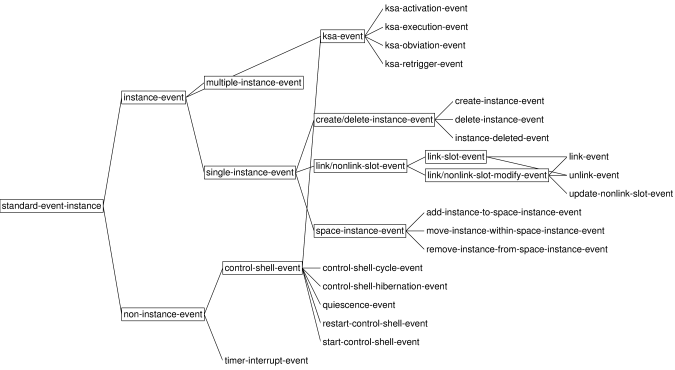
\includegraphics[scale=0.85]{agenda-shell-events}
\end{center}
\W\end{iftex}

\noindent Event classes shown within rectangles are abstract event classes
that cannot be signaled.  Nevertheless, abstract event classes are
very convenient if we wish to attach an event function to an entire
subtree of event classes.  We used abstract event classes to advantage
earlier when we enabled display of all control-shell events by
evaluating:
%
\begin{example}\color{darkergray}%
  gbbopen-user> (enable-event-printing '(control-shell-event :plus-subevents))
  nil
  gbbopen-user>
\end{example}


Add the following form at the end of your \code{tutorial-example.lisp} file:
%
\begin{example}
(add-event-function 'initializations 'start-control-shell-event
                    ;; Initializations should be done first!
                    :priority 100)
\end{example}

(We'll place the \textbf{add-event-function} form immediately after the
\code{initializations} function definition in our file, but this choice of
location is purely a code organizational style preference---the form could be
placed anywhere relative to the function definition.)

\subsection*{Step 3: Run the application}

\bfindex{start-control-shell}%
Start a fresh Common Lisp session, compile and load the
\code{tutorial-example.lisp} file directly from the editor buffer (using
\code{C-c C-k} in SLIME; \code{C-c C-b} in ELI) and start the Agenda Shell
again:
%
\begin{example}\color{darkergray}%
  gbbopen-user> \textcolor{black}{(start-control-shell)}
  ;; Control shell 1 started
  ;; No executable KSAs remain, exiting control shell
  ;; Control shell 1 exited: 3 cycles completed
  ;; Run time: 0 seconds
  ;; Elapsed time: 0 seconds
  :quiescence
  gbbopen-user>
\end{example}

Note that our developing application performs the same as it did in the last
exercise, but now our \code{initializations} event function is taking care of
all the details of starting up our application.  We no longer have to remember
to create the \code{known-world} space instance or to delete the blackboard
repository before running the application another time.

\subsection*{Step 4: Run it Again}

\bfindex{start-control-shell}%
Let's verify that we can re-run our application. Without doing anything else,
start the Agenda Shell again:
%
\begin{example}\color{darkergray}%
  gbbopen-user> \textcolor{black}{(start-control-shell)}
  ;; Control shell 1 started
  ;; No executable KSAs remain, exiting control shell
  ;; Control shell 1 exited: 3 cycles completed
  ;; Run time: 0 seconds
  ;; Elapsed time: 0 seconds
  :quiescence
  gbbopen-user>
\end{example}

As before our \code{initializations} event function took care of all the
details of starting up our application.

\subsection*{Step 5: It's a new world$\ldots$}

\bfindexit{make-space-instance}%
GBBopen allows us to restrict the classes of unit instances that can be stored
on a space instance.  For example, we can limit the \code{known-world} to
\code{location} unit instances by specifying an \code{:allowed-unit-classes}
value to \code{make-space-instance}:
%
\begin{example}\color{darkergray}%
  (defun initializations (event-name &key &allow-other-keys)
    (declare (ignore event-name))
    ;; Clean up any previous run:
    (delete-blackboard-repository)
    ;; Make a new known-world space instance:
    (make-space-instance 
     '(known-world)
     :dimensions '((x :ordered) (y :ordered))
     \textcolor{black}{:allowed-unit-classes 'location}))
\end{example}
%
Attempting to add any unit-instance that is not a \code{location} to
\code{known-world} will now generate an error.

It is often convenient to specify the dimensions of a space-instance relative
to those of one or more unit classes.  Edit the definition of
\code{initializations}, removing the \code{x} and \code{y} dimensions
specification:
%
\begin{example}\color{darkergray}%
(defun initializations (event-name &key &allow-other-keys)
  (declare (ignore event-name))
  ;; Clean up any previous run:
  (delete-blackboard-repository)
  ;; Make a new known-world space instance:
  (make-space-instance 
   '(known-world)
   :dimensions \textcolor{red}{'((x :ordered) (y :ordered))}
   :allowed-unit-classes 'location))
\end{example}
%
and replacing it with a call of \textbf{dimensions-of} to
obtain the dimensions associated with instances of the \code{location}
unit class:
%
\begin{example}\color{darkergray}%
(defun initializations (event-name &key &allow-other-keys)
  (declare (ignore event-name))
  ;; Clean up any previous run:
  (delete-blackboard-repository)
  ;; Make a new known-world space instance:
  (make-space-instance 
   '(known-world)
   :dimensions \textcolor{black}{(dimensions-of 'location)}
   :allowed-unit-classes 'location))
\end{example}

\subsection*{Step 6: Run the application again}

Compile and load the \code{tutorial-example.lisp} file directly from the
editor buffer (using \code{C-c C-k} in SLIME; \code{C-c C-b} in ELI) and start
the Agenda Shell again:
%
\begin{example}\color{darkergray}%
  gbbopen-user> \textcolor{black}{(start-control-shell)}
  ;; Control shell 1 started
  ;; No executable KSAs remain, exiting control shell
  ;; Control shell 1 exited: 3 cycles completed
  ;; Run time: 0 seconds
  ;; Elapsed time: 0 seconds
  :quiescence
  gbbopen-user>
\end{example}

\bfindexit{describe-space-instance}%
Verify the dimensionality of the \code{known-world} space instance by evaluating:
%
\begin{example}\color{darkergray}%
  gbbopen-user> \textcolor{black}{(describe-space-instance '(known-world))}
  Standard-space-instance #<standard-space-instance (known-world)>
    Allowed unit classes: t
    Dimensions:
      (x :ordered)
      (y :ordered)
  gbbopen-user>
\end{example}

%% ========================================================================
%%  Define Another KS

\T\markright{}%
\T\pagestyle{plain}
\T\cleardoublepage
\W\xname{tutorial-another-ks}
\T\pagestyle{fancy}
\T\thispagestyle{fancybottom}
\T\renewcommand{\headrulewidth}{0pt}
\section{Add Another KS}
\label{sec:another-ks}%

The last exercise made it easy to initialize and run our application
repeatedly by simply starting the Agenda Shell.  We also specified the
dimensionality of our \code{known-world} space instance relative to the
dimensional specifications of the \code{location} unit class.  With these
niceties in place, its time to move beyond our initial \code{location} unit
instance.

\fndocrule

This exercise shows you how to:
\begin{tightitemize}
\item Add an additional dimension to a unit class
\item Define a KS that obtains its execution-context information from its
  triggering unit instance
\item Extend the random-walk application to do some walking
\item Explore the resulting random walk
\end{tightitemize}

\fndocrule

\subsection*{Prerequisites}

\begin{tightitemize}
\item The \code{tutorial-example.lisp} file as modified thus far:
\end{tightitemize}

\begin{example}
(in-package :gbbopen-user)

(define-unit-class location ()
  (x y)
  (:dimensional-values
    (x :point x)
    (y :point y))
  (:initial-space-instances (known-world)))

(defmethod print-instance-slots ((location location) stream)
  (call-next-method)
  (when (and (slot-boundp location 'x)
             (slot-boundp location 'y))
    (format stream " (~s ~s)"
            (x-of location)
            (y-of location))))

;;; ======================================================================
;;;   Startup KS

(defun startup-ks-function (ksa)
  (declare (ignore ksa))
  ;; Create an initial location unit instance at (0,0):
  (make-instance 'location :x 0 :y 0))

(define-ks startup-ks
    :trigger-events ((start-control-shell-event))
    :execution-function 'startup-ks-function)

;;; ======================================================================
;;;   Initializations (run at Agenda Shell startup)

(defun initializations (event-name &key &allow-other-keys)
  (declare (ignore event-name))
  ;; Clean up any previous run:
  (delete-blackboard-repository)
  ;; Make a new known-world space instance:
  (make-space-instance 
   '(known-world)
   :dimensions (dimensions-of 'location)))

(add-event-function 'initializations 'start-control-shell-event
                    ;; Initializations should be done first!
                    :priority 100)
\end{example}

\begin{tightitemize}
\item The \code{:agenda-shell-user} module is loaded
\end{tightitemize}

\subsection*{Step 1: Add  another dimension}

It's time we introduce the notion of time to our application.  Edit the
\code{location} unit-class definition in \code{tutorial-example.lisp}, adding
a new slot, \code{time}, to the \code{location} unit class definition and a
corresponding \code{time} dimensional value:
%
\begin{example}\color{darkergray}%
(define-unit-class location ()
  (\textcolor{black}{time} 
   x y)
  (:dimensional-values
    \textcolor{black}{(time :point time)}
    (x :point x)
    (y :point y))
  (:initial-space-instances (known-world)))
\end{example}

Recall that we specified that the dimensions of the \code{known-world} space
instance that is created by our \code{initializations} function relative to
the dimensions of the \code{location} unit class:
%
\begin{example}\color{darkergray}%
  (make-space-instance 
      '(known-world)
      :dimensions (dimensions-of 'location)))
\end{example}
%
Therefore, we don't need to modify our call to \code{make-space-instance} in
order to add \code{time} as a dimension of \code{known-world}.

Next, modify \code{startup-ks-function} in \code{tutorial-example.lisp} so
that it creates the initial \code{location} unit instance at time 0:
%
\begin{example}\color{darkergray}%
(defun startup-ks-function (ksa)
  (declare (ignore ksa))
  ;; Create an initial location unit instance at (0,0) \textcolor{black}{at time 0}:
  (make-instance 'location \textcolor{black}{:time 0} :x 0 :y 0))
\end{example}

\subsection*{Step 2: A test of time}

Let's check our work.  Compile and load the
\code{tutorial-example.lisp} file directly from the editor buffer (using
\code{C-c C-k} in SLIME; \code{C-c C-b} in ELI) and start the Agenda Shell
again:
%
\begin{example}\color{darkergray}%
  gbbopen-user> \textcolor{black}{(start-control-shell)}
  ;; Control shell 1 started
  ;; No executable KSAs remain, exiting control shell
  ;; Control shell 1 exited: 3 cycles completed
  ;; Run time: 0 seconds
  ;; Elapsed time: 0 seconds
  :quiescence
  gbbopen-user>
\end{example}

\bfindexit{describe-instance}%
\bfindexit{find-instance-by-name}%
Check that the initial \code{location} unit instance is at \code{time} zero:
%
\begin{example}\color{darkergray}%
  gbbopen-user> \textcolor{black}{(describe-instance (find-instance-by-name 1 'location))}
  Location #<location 1 (0 0)>
    Instance name: 1
    Space instances: ((known-world))
    Dimensional values:
      time:  0
      x:  40
      y:  60
    Non-link slots:
      time:  0
      x:  40
      y : 60
    Link slots: None
  gbbopen-user>
\end{example}

\subsection*{Step 3: Define another KS}

Define a KS called \code{random-walk-ks} that:

\begin{tightitemize}
\item Is triggered when a \code{location} unit instance is created
\item Has a constant KSA rating of 100
\item Has an execution function called \code{random-walk-ks-function}, which:
\begin{tightitemize}
\item Checks if we've already walked for 75 locations and prints a message if
  we have. 
\item Otherwise:
\begin{tightitemize}
\item Determines a random location for which the x and y values are within 10
  of the x and y values of the triggering unit instance (that is, the
  \code{location} instance whose creation triggered the \code{random-walk-ks}
  KS)
\item If both of the x and y values for the new random location are between
  -50 and 50, creates a \code{location} unit instance at the random location;
  otherwise, prints a message indicating that we've walked off the world
\end{tightitemize}
\end{tightitemize}
\end{tightitemize}

\subsubsection*{Step 3a: Define a utility function}

Begin implementing the \code{random-walk-ks} by adding the following
utility function to the end of your \code{tutorial-example.lisp} file:

\begin{example}
;;; ======================================================================
;;;   Random-walk KS

(defun add-linear-variance (value max-variance)
  ;;; Returns a new random value in the interval
  ;;; [(- value max-variance), (+ value max-variance)]
  (+ value (- (random (1+ (* max-variance 2))) max-variance)))
\end{example}

Then compile the definition (using \code{C-c C-c} in SLIME or \code{C-c
  C-x} in ELI) and evaluate the following test in the REPL:

\bfindex{printv}%
\begin{example}\color{darkergray}%
  gbbopen-user> \textcolor{black}{(dotimes (i 15) (printv (add-linear-variance 0 10)))}
  ;;  (add-linear-variance 0 10) => 8
  ;;  (add-linear-variance 0 10) => 9
  ;;  (add-linear-variance 0 10) => 4
  ;;  (add-linear-variance 0 10) => 3
  ;;  (add-linear-variance 0 10) => -4
  ;;  (add-linear-variance 0 10) => -10
  ;;  (add-linear-variance 0 10) => -1
  ;;  (add-linear-variance 0 10) => 0
  ;;  (add-linear-variance 0 10) => 4
  ;;  (add-linear-variance 0 10) => 5
  ;;  (add-linear-variance 0 10) => 8
  ;;  (add-linear-variance 0 10) => -5
  ;;  (add-linear-variance 0 10) => -3
  ;;  (add-linear-variance 0 10) => 7
  ;;  (add-linear-variance 0 10) => 6
  nil
  gbbopen-user>
\end{example}

Because \code{add-linear-variance} is stochastic, your results will be
similar but not identical.  Note that we used GBBopen's \textbf{printv}
macro to display the result of each generated value.  \textbf{Printv} can
greatly assist debugging by printing forms and the results of evaluating
them.  \textbf{Printv} can be transparently wrapped around any form in a
complex function definition, as it evaluates and displays all the forms in
its body and returns the values resulting from evaluating the last form:

\begin{example}\color{darkergray}%
  gbbopen-user>  (printv "Some multiple values" (values 1 2) "Some more" (values 3 4 5))
  ;; Some multiple values
  ;;  (values 1 2) => 1; 2
  ;; Some more
  ;;  (values 3 4 5) => 3; 4; 5
  4
  5
  6
  gbbopen-user>
\end{example}

\subsubsection*{Step 3b: Define the \code{random-walk-ks} execution function}

Next add the following KS-execution function to the end of your
\code{tutorial-example.lisp} file:

\begin{example}
(defun random-walk-ks-function (ksa)
  ;;; Move to the next (random) location in the world
  (let* ((trigger-instance (sole-trigger-instance-of ksa))
         ;; The new time is one greater than the stimulus instance's time:
         (time (1+ (time-of trigger-instance))))
    (cond
     ;; If the maximum time value (75) is reached, tell the user we've
     ;; walked too long:
     ((>= time 75) (format t "~2&Walked too long.~\%"))
     (t ;; The new location is +/- 10 of the stimulus instance's location:
      (let ((x (add-linear-variance (x-of trigger-instance) 10))
            (y (add-linear-variance (y-of trigger-instance) 10)))
        (cond
         ;; Check that the new location is within the known-world
         ;; boundaries.  If so, create the new location instance:
         ((and (<= -50 x 50) (<= -50 y 50))
          (make-instance 'location 
            :time time 
            :x x 
            :y y))
         ;; Otherwise, tell the user that we've walked too far away:
         (t (format t "~2\&Walked off the world: (~d, ~d).~\%" x y))))))))
\end{example}

\bfindex{sole-trigger-instance-of}%
Unlike the KS-execution functions that we have defined previously,
\code{random-walk-ks-function} does not ignore its \code{ksa} argument.
Instead, it calls \textbf{sole-trigger-instance-of} with the \code{ksa}
unit-instance argument in order to obtain the \code{location} unit instance
whose creation triggered the KSA.  This pattern of obtaining the unit instance
that triggered a KSA and then using that triggering unit instance as the
context for the KS execution is typical of many KSs. 

\subsubsection*{Step 3c: Add the \code{random-walk-ks} definition}

Finally, add this \code{define-ks} form to the end of your
\code{tutorial-example.lisp} file to complete the \code{random-walk-ks}
definition:

\bfindexit{define-ks}%
\codeindex{quiescence-event}%
\begin{example}
(define-ks random-walk-ks
   :trigger-events ((create-instance-event location))
   :rating 100
   :execution-function 'random-walk-ks-function)
\end{example}

\subsection*{Step 4:  Run the application}

\bfindexit{start-control-shell}%
Compile and load the \code{random-walk-ks} forms, and then start the Agenda Shell:
%
\begin{example}\color{darkergray}%
  gbbopen-user> \textcolor{black}{(start-control-shell)}
  ;; Control shell 1 started

  Walked off the world: (23, 55).
  ;; No executable KSAs remain, exiting control shell
  ;; Control shell 1 exited: 64 cycles completed
  ;; Run time: 0.01 seconds
  ;; Elapsed time: 0 seconds
  :quiescence
  gbbopen-user>
\end{example}

\bfindexit{:dsbb}%
It looks like something happened! (Again, because \code{add-linear-variance}
is stochastic, your results will be similar but not identical.)  Let's look at
the blackboard repository and see how many \code{location} unit instances were
created:
%
\begin{example}\color{darkergray}%
  gbbopen-user> \textcolor{black}{:dsbb}

  Space Instance                Contents
  --------------                --------
  known-world                   61 instances (61 location)

  Unit Class                    Instances
  ----------                    ---------
  control-shell                         1 *
  ks                                    1 +
  ksa-queue                             2 +
  location                             61
  ordered-ksa-queue                     1 +
  standard-space-instance               1
                                ---------
                                       67 instances
  gbbopen-user>
\end{example}

The 61 \code{location} instances makes sense.  Previously, it required 3
control-shell cycles to create the initial \code{location} unit instance (one
to execute the \code{initial-ks} KSA followed by two additional cycles of
quiescence before the Agenda Shell exits).  We now create one additional
\code{location} unit instance with every execution of \code{random-walk-ks},
so we always create 3 fewer \code{location} instances than the total
number of control-shell cycles.

\subsection*{Step 5:  Where have we been?}

\bfindexit{map-instances-of-class}%
It would be interesting to see where our random walk has taken us.  We could
use GBBopen's \textbf{map-instances-of-class} iterator to print each of the
\code{location} unit instances:
%
\begin{example}\color{darkergray}%
  gbbopen-user> \textcolor{black}{(map-instances-of-class #'print 'location)}

  #<location 58 (5 31)> 
  #<location 13 (-7 10)> 
  #<location 26 (-40 35)> 
  #<location 39 (-4 3)> 
  #<location 52 (2 23)> 
  #<location 7 (3 17)> 
  #<location 20 (2 27)> 
  #<location 33 (-25 6)> 
  #<location 46 (-2 32)> 
       ...
  #<location 31 (-22 18)> 
  #<location 44 (-7 14)> 
  #<location 57 (2 41)> 
  #<location 12 (-15 15)> 
  #<location 25 (-32 38)> 
  #<location 38 (-10 -4)> 
  #<location 51 (-2 16)> 
  #<location 6 (10 27)> 
  #<location 19 (-1 17)> 
  #<location 32 (-25 12)> 
  #<location 45 (-7 23)> 
  nil
  gbbopen-user>
\end{example}
%
Unfortunately, the order that unit instances are supplied to the \code{print}
function is not controllable.  Our walk would be much clearer if we printed
the \code{location}s in time order.

\bfindexit{map-sorted-instances-of-class}%
We might consider taking advantage of the instance names that GBBopen assigns
to unit instances.  We could do something like the following:
%
\begin{example}\color{darkergray}%
  gbbopen-user> \textcolor{red}{(dotimes (i 76)
                  (let ((location (find-instance-by-name i 'location)))
                    (when location
                       (print location))))}

  #<location 1 (0 0)> 
  #<location 2 (10 4)> 
  #<location 3 (19 10)> 
  #<location 4 (14 9)> 
  #<location 5 (14 18)> 
  #<location 6 (10 27)> 
  #<location 7 (3 17)> 
  #<location 8 (-6 20)> 
  #<location 9 (4 15)> 
  #<location 10 (-5 14)> 
       ...
  #<location 50 (5 26)> 
  #<location 51 (-2 16)> 
  #<location 52 (2 23)> 
  #<location 53 (9 33)> 
  #<location 54 (7 43)> 
  #<location 55 (-2 36)> 
  #<location 56 (0 46)> 
  #<location 57 (2 41)> 
  #<location 58 (5 31)> 
  #<location 59 (13 39)> 
  #<location 60 (17 41)> 
  #<location 61 (21 50)> 
  nil
  gbbopen-user>
\end{example}

This is a bad idea for several reasons.  First, we are looking up every
\code{location} unit instance by its instance name, which is less efficient
than operating on \code{location} instances directly.  While this isn't an
significant issue in expressions that we evaluate in the REPL to investigate
our application, we should seek to avoid such inefficiencies in application
code.  More importantly, however, the \code{location} instance name just
happens to mirror the sequencing that we really want to display---the
\code{time} value of the \code{location}s.  We should find a way to sequence
\code{location} printing that relies on the \code{time} values directly.

\bfindex{map-sorted-instances-of-class}%
GBBopen provides a variant of \textbf{map-instances-of-class}, called
\textbf{map-sorted-instances-of-class}, that sorts the unit instances based on
a comparison predicate and an optional \code{:key} accessor function that
suits our needs:
%
\begin{example}\color{darkergray}%
  gbbopen-user> \textcolor{black}{(map-sorted-instances-of-class #'print 'location #'< 
                   :key #'time-of)}

  #<location 1 (0 0)> 
  #<location 2 (10 4)> 
  #<location 3 (19 10)> 
  #<location 4 (14 9)> 
  #<location 5 (14 18)> 
  #<location 6 (10 27)> 
  #<location 7 (3 17)> 
  #<location 8 (-6 20)> 
  #<location 9 (4 15)> 
  #<location 10 (-5 14)> 
       ...
  #<location 50 (5 26)> 
  #<location 51 (-2 16)> 
  #<location 52 (2 23)> 
  #<location 53 (9 33)> 
  #<location 54 (7 43)> 
  #<location 55 (-2 36)> 
  #<location 56 (0 46)> 
  #<location 57 (2 41)> 
  #<location 58 (5 31)> 
  #<location 59 (13 39)> 
  #<location 60 (17 41)> 
  #<location 61 (21 50)> 
  nil
  gbbopen-user>
\end{example}

\bfindex{do-sorted-instances-of-class}%
Using \textbf{map-sorted-instances-of-class} involves a sorting operation, so
this approach still has some efficiency concerns for use in application code.
However, it suits our REPL-exploration needs just fine.  (There is a
\textbf{do-sorted-instances-of-class} macro, if an iterative style is
preferred over a mapper.)  We will explore a more efficient approach to
displaying the random walk in the next exercise.

\subsection*{Step 6:  Run the application a few more times}

\bfindexit{start-control-shell}%
If we run the application a few more times, we eventually encounter a case
where we create the allotted 75 \code{location} unit instances without walking
off the \code{known-world}:
%
\begin{example}\color{darkergray}%
  gbbopen-user> \textcolor{black}{(start-control-shell)}
  ;; Control shell 1 started

  Walked too long.
  ;; No executable KSAs remain, exiting control shell
  ;; Control shell 1 exited: 78 cycles completed
  ;; Run time: 0.04 seconds
  ;; Elapsed time: 0 seconds
  :quiescence
  gbbopen-user>
\end{example}

\bfindexit{map-sorted-instances-of-class}%
Here is one such random walk:
%
\begin{example}\color{darkergray}%
  gbbopen-user> \textcolor{black}{(map-sorted-instances-of-class #'print 'location #'< 
                   :key #'time-of)}

  #<location 1 (0 0)> 
  #<location 2 (2 7)> 
  #<location 3 (-1 5)> 
  #<location 4 (-1 0)> 
  #<location 5 (3 -2)> 
  #<location 6 (13 -7)> 
  #<location 7 (8 -5)> 
  #<location 8 (1 2)> 
  #<location 9 (8 0)> 
  #<location 10 (5 8)> 
       ...
  #<location 70 (-13 -11)> 
  #<location 71 (-13 -6)> 
  #<location 72 (-9 -6)> 
  #<location 73 (1 -4)> 
  #<location 74 (-8 -11)> 
  #<location 75 (-13 -15)> 
  nil
  gbbopen-user>
\end{example}

%% ========================================================================
%%  Making Connections

\T\markright{}%
\T\pagestyle{plain}
\T\cleardoublepage
\W\xname{tutorial-connections}
\T\pagestyle{fancy}
\T\thispagestyle{fancybottom}
\T\renewcommand{\headrulewidth}{0pt}
\section{Making Connections}
\label{sec:connections}%

%\begin{center}
%\textcolor{caution}{[Construction ahead...]}
%\end{center}

We finally did some walking in the last exercise and learned how to display
the \code{location}s in our walk from the REPL.  In this exercise, we learn
how to use GBBopen's link capabilities to represent relationships among unit
instances.  Links are an important aspect of almost every GBBopen application,
so it's time that we started taking advantage of them.

\fndocrule

This exercise shows you how to:
\begin{tightitemize}
\item Add link slots to a unit class
\item Use link slots to traverse and display the resulting random walk
\end{tightitemize}

\fndocrule

\subsection*{Prerequisites}

\begin{tightitemize}
\item The \code{tutorial-example.lisp} file as modified thus far:
\end{tightitemize}

\begin{example}
(in-package :gbbopen-user)

(define-unit-class location ()
  (time 
   x y)
  (:dimensional-values
    (time :point time)
    (x :point x)
    (y :point y))
  (:initial-space-instances (known-world)))

(defmethod print-instance-slots ((location location) stream)
  (call-next-method)
  (when (and (slot-boundp location 'x)
             (slot-boundp location 'y))
    (format stream " (~s ~s)"
            (x-of location)
            (y-of location))))

;;; ======================================================================
;;;   Startup KS

(defun startup-ks-function (ksa)
  (declare (ignore ksa))
  ;; Create an initial location unit instance at (0,0):
  (make-instance 'location :time 0 :x 0 :y 0))

(define-ks startup-ks
    :trigger-events ((start-control-shell-event))
    :execution-function 'startup-ks-function)

;;; ======================================================================
;;;   Initializations (run at Agenda Shell startup)

(defun initializations (event-name &key &allow-other-keys)
  (declare (ignore event-name))
  ;; Clean up any previous run:
  (delete-blackboard-repository)
  ;; Make a new known-world space instance:
  (make-space-instance 
   '(known-world)
   :dimensions (dimensions-of 'location)))

(add-event-function 'initializations 'start-control-shell-event
                    ;; Initializations should be done first!
                    :priority 100)

;;; ======================================================================
;;;   Random-walk KS

(defun add-linear-variance (value max-variance)
  ;;; Returns a new random value in the interval
  ;;; [(- value max-variance), (+ value max-variance)]
  (+ value (- (random (1+ (* max-variance 2))) max-variance)))

(defun random-walk-ks-function (ksa)
  ;;; Move to the next (random) location in the world
  (let* ((trigger-instance (sole-trigger-instance-of ksa))
         ;; The new time is one greater than the stimulus instance's time:
         (time (1+ (time-of trigger-instance))))
    (cond
     ;; If the maximum time value (75) is reached, tell the user we've
     ;; walked too long:
     ((>= time 75) (format t "~2&Walked too long.~\%"))
     (t ;; The new location is +/- 10 of the stimulus instance's location:
      (let ((x (add-linear-variance (x-of trigger-instance) 10))
            (y (add-linear-variance (y-of trigger-instance) 10)))
        (cond
         ;; Check that the new location is within the known-world
         ;; boundaries.  If so, create the new location instance:
         ((and (<= -50 x 50) (<= -50 y 50))
          (make-instance 'location 
            :time time 
            :x x 
            :y y))
         ;; Otherwise, tell the user that we've walked too far away:
         (t (format t "~2&Walked off the world: (~d, ~d).~\%" x y))))))))

(define-ks random-walk-ks
    :trigger-events ((create-instance-event location))
    :rating 100
    :execution-function 'random-walk-ks-function)
\end{example}

\begin{tightitemize}
\item The \code{:agenda-shell-user} module is loaded
\end{tightitemize}

\subsection*{Step 1: Add  a link}

In the last exercise, we used \textbf{map-sorted-instances-of-class} to
display the random walk.  Another way that we could represent the walk is by
connect each newly created \code{location} unit instance to the
\code{location} unit instance that preceded it in the walk.  We'll use
GBBopen's link capabilities to do this.

A \textit{link} is a bidirectional relationship between two unit instances
that is implemented by two pointers. From the perspective of a particular unit
instance, each link consists of an outgoing, or \textit{direct}, pointer to
another unit instance and an incoming, or \textit{inverse}, pointer that is
stored in unit instance pointed to by the direct pointer.  GBBopen
automatically maintains the bidirectional-link consistency of these pointers
when creating new links, deleting existing links, or deleting unit instances.
Links remove the possibility of ``one-sided'' relationships or ``dangling''
pointers to deleted unit instances.

Edit the \code{location} unit-class definition in your
\code{tutorial-example.lisp} file, adding two link slots, \code{next-location}
and \code{previous-location}, to the \code{location} unit class definition:
%
\begin{example}\color{darkergray}%
(define-unit-class location ()
  (time 
   x y
   \textcolor{black}{(next-location
    :link (location previous-location :singular t) 
    :singular t)
   (previous-location
    :link (location next-location :singular t)  
    :singular t)})
  (:dimensional-values
    (time :point time)
    (x :point x)
    (y :point y))
  (:initial-space-instances (known-world)))
\end{example}

Each link-slot specification is a list whose first element is the name of the
link slot.  This is followed by the link slot option \code{:link} and a
concise specification of the inverse link slot associated with that link slot.
In this case, the \code{next-location}/\code{previous-location} link is
between instances of the same (\code{location}) unit class, but often links
are between instances of different unit classes. 

Links can be many-to-many, many-to-one, one-to-many, or one-to-one.  In this
case, the \code{next-location}/\code{previous-location} link is one-to-one,
which is specified by including the \code{:singular t} slot option in the
link-slot definition (and the corresponding \code{:singular t} specification
in the concise inverse-link-slot specification).  To help clarify the
specification of link slot arity, let's temporarily assume that we want a
\code{location} instance that can have many next locations, but only a single
previous location.  This link relation would be specified as follows:
%
\begin{example}\color{darkergray}%
    ...
 \textcolor{blue}{(next-locations
  :link (location previous-location :singular t)))
 (previous-location
  :link (location next-locations)  
  :singular t)}
    ...
\end{example}

We've followed the natural GBBopen convention of giving singular link
slots a singular name (such as \code{previous-location}) and link
slots that can contain multiple links a plural name (such as
\code{next-locations}).  Note that the \code{:singular} option is
associated with the \code{previous-location} link slot as both a slot
option in the \code{previous-location} link-slot definition and in the
concise inverse-link-slot specification for \code{previous-location}
in the \code{next-locations} link-slot definition.

\subsection*{Step 2: Break some links}

The concise inverse-link-slot specification supplied by the
\code{:link} slot option provides a ``double entry'' redundancy that
is useful when links are between instances of different unit classes,
as the link can be understood by viewing either class definition.  The
redundancy also helps GBBopen recognize inconsistencies in link
specifications.  The function \textbf{check-link-consistency} asks
GBBopen to validate that all link definitions are consistent.  Let's
try it on our current random-walk application.  Compile and load the
latest changes in your \code{tutorial-example.lisp} file (including
the new \code{next-location} and \code{previous-location} link slots).
Then check link consistency:
%
\begin{example}\color{darkergray}%
  gbbopen-user> \textcolor{black}{(check-link-consistency)}
  ;; All link definitions are consistent.
  t
  gbbopen-user>
\end{example}
%
GBBopen reports that all link definitions are consistent.

Suppose that we had forgotten to add the \code{previous-location} end
of the link in our \code{location} unit-class definition. Edit the
\code{location} unit-class definition in your
\code{tutorial-example.lisp} file, adding the line \code{\#+ignore}
immediately before the \code{previous-location} link-slot definition:
%
\begin{example}\color{darkergray}%
(define-unit-class location ()
  (time 
   x y
   (next-location
    :link (location previous-location :singular t) 
    :singular t)
    \textcolor{black}{\#+ignore}     
   (previous-location
    :link (location next-location :singular t)  
    :singular t))
  (:dimensional-values
    (time :point time)
    (x :point x)
    (y :point y))
  (:initial-space-instances (known-world)))
\end{example}

The \code{\#+ignore} read-time conditionalization tells Common Lisp to
skip over the next form if \code{ignore} is not an element of the
feature list \code{*features*}.  By convention, \code{ignore} is never
added to \code{*features*}, so \code{\#+ignore} is a handy mechanism
for temporarily ``commenting out'' a single form.

Compile the now-defective definition (using \code{C-c C-c} in SLIME or
\code{C-c C-x} in ELI) and then recheck link consistency:
%
\begin{example}\color{darkergray}%
  gbbopen-user> \textcolor{black}{(check-link-consistency)}
  Warning: The inverse of link slot next-location in unit class location 
           refers to link slot previous-location which is not present in 
           unit class location.
  nil
  gbbopen-user>
\end{example}
%
As expected, GBBopen alerts us to the problem.

Remove the \code{\#+ignore} that we just added and comment out the
\code{:singular t} portion of the inverse link-slot specification in 
\code{next-location}:
%
\begin{example}\color{darkergray}%
(define-unit-class location ()
  (time 
   x y
   (next-location
    :link (location previous-location\textcolor{black}{) ;} :singular t) 
    :singular t)
    \textcolor{red}{#+ignore}     
   (previous-location
    :link (location next-location :singular t)  
    :singular t))
  (:dimensional-values
    (time :point time)
    (x :point x)
    (y :point y))
  (:initial-space-instances (known-world)))
\end{example}

Compile the again-defective definition (using \code{C-c C-c} in SLIME or
\code{C-c C-x} in ELI) and then recheck link consistency:
%
\begin{example}\color{darkergray}%
  gbbopen-user> \textcolor{black}{(check-link-consistency)}
  Warning: Link slot next-location in unit class location incorrectly 
           declares its inverse link slot previous-location in unit 
           class location as not singular.
  nil
  gbbopen-user>
\end{example}
%
Once again, GBBopen has alerted us to the problem.

Restore the \code{:singular t} portion of the inverse link-slot
specification in \code{next-location} that we just commented out:
%
\begin{example}\color{darkergray}%
(define-unit-class location ()
  (time 
   x y
   (next-location
    :link (location previous-location\textcolor{red}{) ;} :singular t) 
    :singular t)
   (previous-location
    :link (location next-location :singular t)  
    :singular t))
  (:dimensional-values
    (time :point time)
    (x :point x)
    (y :point y))
  (:initial-space-instances (known-world)))
\end{example}

Then recompile and recheck link consistency:
%
\begin{example}\color{darkergray}%
  gbbopen-user> \textcolor{black}{(check-link-consistency)}
  ;; All link definitions are consistent.
  t
  gbbopen-user>
\end{example}

\subsection*{Step 3: Create some links}

Let's use our newly defined \code{next-location}/\code{previous-location} link
to connect our \code{location} unit instances.  Edit the
\code{random-walk-ks-function} definition in your \code{tutorial-example.lisp}
file, adding the trigger instance as a new \code{:previous-location} argument
to \code{make-instance}:
%
\begin{example}\color{darkergray}%
(defun random-walk-ks-function (ksa)
  ;;; Move to the next (random) location in the world
  (let* ((trigger-instance (sole-trigger-instance-of ksa))
         ;; The new time is one greater than the stimulus instance's time:
         (time (1+ (time-of trigger-instance))))
    (cond
     ;; If the maximum time value (75) is reached, tell the user we've
     ;; walked too long:
     ((>= time 75) (format t "~2&Walked too long.~\%"))
     (t ;; The new location is +/- 10 of the stimulus instance's location:
      (let ((x (add-linear-variance (x-of trigger-instance) 10))
            (y (add-linear-variance (y-of trigger-instance) 10)))
        (cond
         ;; Check that the new location is within the known-world
         ;; boundaries.  If so, create the new location instance:
         ((and (<= -50 x 50) (<= -50 y 50))
          (make-instance 'location 
            :time time 
            :x x 
            :y y
            \textcolor{black}{:previous-location trigger-instance}))
         ;; Otherwise, tell the user that we've walked too far away:
         (t (format t "~2&Walked off the world: (~d, ~d).~\%" x y))))))))
\end{example}

Compile the \code{random-walk-ks-function} (using \code{C-c C-c} in SLIME or
\code{C-c C-x} in ELI) and then run the application:
%
\begin{example}\color{darkergray}%
  gbbopen-user> \textcolor{black}{(start-control-shell)}
  ;; Control shell 1 started

  Walked off the world: (55, 35).
  ;; No executable KSAs remain, exiting control shell
  ;; Control shell 1 exited: 66 cycles completed
  ;; Run time: 0.01 seconds
  ;; Elapsed time: 0 seconds
  :quiescence
  gbbopen-user>
\end{example}

Let's describe a couple of \code{location} unit instances to check our work.
First, the initial \code{location} unit instance:
%
\begin{example}\color{darkergray}%
  gbbopen-user> \textcolor{black}{(describe-instance (find-instance-by-name 1 'location))}
  Location #<location 1 (0 0)>
    Instance name: 1
    Space instances: ((known-world))
    Dimensional values:
      time:  0
      x:  40
      y:  60
    Non-link slots:
      time:  0
      x:  40
      y:  60
    Link slots:
      next-location:  #<location 2 (-10 10)>
      previous-location:  nil
  gbbopen-user>
\end{example}

Note that the \code{next-location} link slot points to the next
\code{location} unit instance in our random walk.  Let's describe that
unit instance:
%
\begin{example}\color{darkergray}%
  gbbopen-user> \textcolor{black}{(describe-instance (find-instance-by-name 2 'location))}
  Location #<location 2 (-10 10)>
    Instance name: 2
    Space instances: ((known-world))
    Dimensional values:
      time:  1
      x:  -10
      y:  10
    Non-link slots:
      time:  1
      x:  -10
      y:  10
    Link slots:
      next-location:  #<location 3 (-6 19)>
      previous-location:  #<location 1 (0 0)>
  gbbopen-user>
\end{example}

Its \code{next-location} link slot points to the third \code{location} unit
instance in our random walk and its \code{previous-location} link slot points
back to the initial \code{location} unit instance.

We can now follow the links to display the random walk:
%
\begin{example}\color{darkergray}%
  gbbopen-user> \textcolor{black}{(loop with location = (find-instance-by-name 1 'location) 
                  do (print location)
                  while (setf location (next-location-of location)))}

  #<location 1 (0 0)> 
  #<location 2 (-10 10)> 
  #<location 3 (-6 19)> 
  #<location 4 (0 14)> 
  #<location 5 (-1 14)> 
  #<location 6 (8 10)> 
  #<location 7 (17 3)> 
  #<location 8 (7 -6)> 
  #<location 9 (10 4)> 
  #<location 10 (5 -5)> 
       ...
  #<location 60 (29 17)> 
  #<location 61 (31 21)> 
  #<location 62 (40 23)> 
  #<location 63 (45 28)> 
  nil
  gbbopen-user>
\end{example}

\subsection*{Step 4: Define a ``print walk'' KS}

\bfindexit{define-ks}%
\codeindex{:stop}%
\codeindex{quiescence-event}%
\bfindexit{find-instance-by-name}%
Let's add a new KS, \code{print-walk-ks}, that displays the random walk once
it is completed. Add the following KS to the end of your
\code{tutorial-example.lisp} file:
%
\begin{example}
;;; ======================================================================
;;;   Print-walk KS

(defun print-walk-ks-function (ksa)
  ;;; Starting with the initial location instance, print the instance name
  ;;; and location of the walk
    (declare (ignore ksa))
    (format t "~2\&The random walk:~\%")
      (let ((instance (find-instance-by-name 1 'location)))
      (while instance
        (format t "~s (~s ~s)~\%"
                (instance-name-of instance)
                (x-of instance)
                (y-of instance))
        (setf instance (next-location-of instance))))
    ;; Tell the Agenda Shell to exit:
    ':stop)

  (define-ks print-walk-ks
    :trigger-events ((quiescence-event))
    :rating 100
    :execution-function 'print-walk-ks-function)
\end{example}
%
The \code{print-walk-ks} is triggered by a \code{quiescence-event}.  Recall
that the Agenda Shell signals that quiescence has occurred when no
executable KSAs are available to be executed and then it continues for an
additional KS-execution cycle in case any executable KSAs resulted from the
quiescence event.  So, \code{print-walk-ks} will be triggered once no
\code{random-walk-ks} KSAs are triggered by newly created \code{location} unit
instances.

The \code{print-walk-ks-function} follows the
\code{next-location}/\code{previous-location} link to display the walk.  More
importantly, the function returns the keyword symbol \code{:stop}.  The Agenda
Shell checks the value returned by a KS execution function for this special
indicator and, if it is returned, the control shell is exited.  If we did not
return \code{:stop}, the \code{print-walk-ks} KS would be triggered and
activated on the first \code{quiescence-event}, the KSA would execute, then
the Agenda Shell would detect another quiescence condition, signal a new
\code{quiescence-event}, and our application would print the random walk over
and over again.

Let's compile our latest changes and then run our application with the new
\code{print-walk-ks} KS in place:
%
\begin{example}\color{darkergray}%
  gbbopen-user> \textcolor{black}{(start-control-shell)}
  ;; Control shell 1 started

  Walked off the world: (54, 15).

  The random walk:
  1 (0 0)
  2 (-6 9)
  3 (-14 8)
  4 (-5 6)
  5 (-13 5)
  6 (-11 13)
  7 (-11 4)
  8 (-17 8)
  9 (-21 15)
  10 (-12 14)
       ...
  35 (40 28)
  36 (50 22)
  37 (49 12)
  38 (47 10)
  ;; Explicit :stop issued by KS print-walk-ks
  ;; Control shell 1 exited: 41 cycles completed
  ;; Run time: 0.01 seconds
  ;; Elapsed time: 0 seconds
  :stop
  gbbopen-user>
\end{example}

%% ========================================================================
%%  Creating an Application

\T\markright{}%
\T\pagestyle{plain}
\T\cleardoublepage
\W\xname{tutorial-application}
\T\pagestyle{fancy}
\T\thispagestyle{fancybottom}
\T\renewcommand{\headrulewidth}{0pt}
\section{Creating a GBBopen Application}
\label{sec:application}%

GBBopen's \xreflink{Mini Module system}{sec:mini-module} provides facilities
that make it easy to define and use your own GBBopen applications.

\fndocrule

This exercise shows you how to:
\begin{tightitemize}
\item Structure an application using the \xreflink{Mini Module
    system}{sec:mini-module}
\item Define a top-level REPL command for your application
\item Compile and load your application using your REPL command
\item Create and use an application-specific package
\item Add an ``autorun'' form 
\end{tightitemize}

\fndocrule

\subsection*{Prerequisites}

\begin{tightitemize}
\item The \code{tutorial-example.lisp} file as modified thus far:

\begin{example}
(in-package :gbbopen-user)

(define-unit-class location ()
  (time 
   x y
   (next-location
    :link (location previous-location :singular t) 
    :singular t)
   (previous-location
    :link (location next-location :singular t)  
    :singular t))
  (:dimensional-values
    (time :point time)
    (x :point x)
    (y :point y))
  (:initial-space-instances (known-world)))

(defmethod print-instance-slots ((location location) stream)
  (call-next-method)
  (when (and (slot-boundp location 'x)
             (slot-boundp location 'y))
    (format stream " (~s ~s)"
            (x-of location)
            (y-of location))))

;;; ======================================================================
;;;   Startup KS

(defun startup-ks-function (ksa)
  (declare (ignore ksa))
  ;; Create an initial location unit instance at (0,0):
  (make-instance 'location :time 0 :x 0 :y 0))

(define-ks startup-ks
    :trigger-events ((start-control-shell-event))
    :execution-function 'startup-ks-function)

;;; ======================================================================
;;;   Initializations (run at Agenda Shell startup)

(defun initializations (event-name &key &allow-other-keys)
  (declare (ignore event-name))
  ;; Clean up any previous run:
  (delete-blackboard-repository)
  ;; Make a new known-world space instance:
  (make-space-instance 
   '(known-world)
   :dimensions (dimensions-of 'location)))

(add-event-function 'initializations 'start-control-shell-event
                    ;; Initializations should be done first!
                    :priority 100)

;;; ======================================================================
;;;   Random-walk KS

(defun add-linear-variance (value max-variance)
  ;;; Returns a new random value in the interval
  ;;; [(- value max-variance), (+ value max-variance)]
  (+ value (- (random (1+ (* max-variance 2))) max-variance)))

(defun random-walk-ks-function (ksa)
  ;;; Move to the next (random) location in the world
  (let* ((trigger-instance (sole-trigger-instance-of ksa))
         ;; The new time is one greater than the stimulus instance's time:
         (time (1+ (time-of trigger-instance))))
    (cond
     ;; If the maximum time value (75) is reached, tell the user we've
     ;; walked too long:
     ((>= time 75) (format t "~2&Walked too long.~\%"))
     (t ;; The new location is +/- 10 of the stimulus instance's location:
      (let ((x (add-linear-variance (x-of trigger-instance) 10))
            (y (add-linear-variance (y-of trigger-instance) 10)))
        (cond
         ;; Check that the new location is within the known-world
         ;; boundaries.  If so, create the new location instance:
         ((and (<= -50 x 50) (<= -50 y 50))
          (make-instance 'location 
            :time time 
            :x x 
            :y y
            :previous-location trigger-instance))
         ;; Otherwise, tell the user that we've walked too far away:
         (t (format t "~2\&Walked off the world: (~d, ~d).~\%" x y))))))))

(define-ks random-walk-ks
    :trigger-events ((create-instance-event location))
    :rating 100
    :execution-function 'random-walk-ks-function)

;;; ======================================================================
;;;   Print-walk KS

(defun print-walk-ks-function (ksa)
  ;;; Starting with the initial location instance, print the instance name
  ;;; and location of the walk
  (declare (ignore ksa))
  (format t "~2\&The random walk:~\%")
    (let ((instance (find-instance-by-name 1 'location)))
    (while instance
      (format t "~s (~s ~s)~\%"
              (instance-name-of instance)
              (x-of instance)
              (y-of instance))
      (setf instance (next-location-of instance))))
  ;; Tell the Agenda Shell to exit:
  ':stop)

(define-ks print-walk-ks
  :trigger-events ((quiescence-event))
  :rating 100
  :execution-function 'print-walk-ks-function)
\end{example}

\item The GBBopen environment setup using
  \code{\var{<install-dir>\/}/gbbopen-init.lisp} as described in Steps 1 and 2
  of the \reflink{Enhancing Your Development Environment
    exercise}{sec:environment}
\end{tightitemize}

\subsection*{Step 1: Create your personal \code{gbbopen-modules} directory}

Create a directory named \code{gbbopen-modules} in your \reflink{``homedir''
  directory}{ref:your-homedir}.  For example:
%
\begin{example}\color{darkergray}%
  [~]\$ \textcolor{black}{mkdir gbbopen-modules}
  [~]\$ 
\end{example}
%
This is a special directory that is read by used by GBBopen to find
applications when GBBopen is started using
\code{\var{<install-dir>\/}/gbbopen-init.lisp}, as described in Steps 1 and 2
of the \reflink{Enhancing Your Development Environment
  exercise}{sec:environment}.

\subsection*{Step 2: Create a module-definition file for the random-walk application}

Recall that you created a directory to hold the random-walk application in Step 1
of \reflink{Working Within a File exercise}{sec:file}.  I used these shell
commands to create my directories:
%
\begin{example}\color{darkergray}%
  [~]\$ mkdir tutorial
  [~]\$ cd tutorial
  [~/tutorial]\$ mkdir source
  [~/tutorial]\$ 
\end{example}
%
Then you created the \code{tutorial-example.lisp} file in this \code{source}
subdirectory. We said that we would explain why we created the \code{source}
directory in a later exercise.  Well, later has arrived.

Each GBBopen application is packaged in a directory that contains:
\begin{tightitemize}
\item a \code{modules.lisp} file that contains module definitions (loaded
  after the personal \code{\var{<install-dir>\/}/gbbopen-init.lisp} file if
  there is one in the user's ``homedir'')
\item a directory named \code{source} containing all the source files for the
  module or application
\item an optional \code{commands.lisp} file that specifies top-level commands
  for the module (loaded after the personal \code{gbbopen-commands.lisp} file
  if there is one in the user's ``homedir'')
\end{tightitemize}
%
You already have the \code{source} directory and the
\code{tutorial-example.lisp} source file.  Next, we create the
\code{modules.lisp} file for the application.  (We will create a
\code{commands.lisp} file for the random-walk application in Step 5.)

Use your Common Lisp editor to create a new file named \code{modules.lisp} in
the \code{tutorial} directory (just as you created the
\code{tutorial-example.lisp} file in Step 2 of \reflink{Working Within a File
  exercise}{sec:file}.  Note that this file is \textit{not\/} in the
\code{source} subdirectory, but in the \code{tutorial} directory that contains
the \code{source} subdirectory.

Type the following two forms into the new \code{modules.lisp}
file:
%
\begin{example}
(in-package :common-lisp-user)

(define-module :tutorial
  (:requires :agenda-shell-user)
  (:files "tutorial-example"))
\end{example}
%
and then save the file.

Recall that the \code{in-package} form specifies the Common Lisp package that
is made current when the file is compiled or loaded.  A \code{modules.lisp}
file should always specify the \code{:mini-module-user} package as the first
form in the file.

The second form defines our application module, which we will name
\code{:tutorial}.  The \code{:requires} subform specifies that the
\code{:agenda-shell-user} module must be compiled (if necessary) and then
loaded before our \code{:tutorial} module.  The \code{:files} subform
specified the files that comprise the module. In our case, there is one file:
\code{tutorial-example.lisp}.  We leave off the \code{.lisp} file extension,
as the \xreflink{Mini Module system}{sec:mini-module} will add the appropriate
source or compiled file extension for us.

\subsection*{Step 3: Add the random-walk application to your personal
  \code{gbbopen-modules} directory}

The \code{gbbopen-modules} directory in your ``homedir'' is expected to
consist of directories each containing an individual GBBopen application.  We
could place the random-walk application directly in the \code{gbbopen-modules}
directory by moving the \code{tutorial} directory there.  However, it is
generally more convenient to use a symbolic link to point to the actual
application directory.  For example, an application can be provided to a
number of users by creating a symbolic link to the application directory in
each user's \code{gbbopen-modules} directory.

Unless you are running Windows, add the random-walk application to your
\code{gbbopen-applications} by creating a symbolic link.  For example:
%
\begin{example}\color{darkergray}%
  [~]\$ \textcolor{black}{cd ~/gbbopen-modules/}
  [~]\$ \textcolor{black}{ln -s ~/tutorial .}
  [~]\$ 
\end{example}

\subsubsection*{Windows users}

Instead of creating a symbolic link, GBBopen also supports a special ``pseudo
symbolic-link'' file that can be used with Windows.  This is simply a text
file of type \code{.sym} that contains the target directory path as the sole
line in the file.  For example, you could create the file \code{tutorial.sym}
in your \code{gbbopen-modules} directory with:
%
\begin{example}
  C:\bkslash{}tutorial\bkslash
\end{example}
\T\vskip -12pt
%
as the sole line in the file.

\subsection*{Step 4: Try the \code{:tutorial} module definition}

Let's try out our module definition.  Exit Common Lisp and start a fresh
Common Lisp session.  If you have set up your environment according to the
\reflink{Enhancing Your Development Environment exercise}{sec:environment},
the following files should be loaded:
%
\begin{example}\color{darkergray}%
     ...
  ;; Loading \var{<homedir\/>}/shared-init.lisp
  ;;   Loading \var{<install-dir\/>}/gbbopen-init.lisp
  ;;     Loading \var{<install-dir\/>}/extended-repl.lisp
  ;;     Loading \var{<install-dir\/>}/commands.lisp
  ;;     Loading \var{<install-dir\/>}/gbbopen-modules-directory.lisp
  ;; Loading module command definitions from \var{<homedir\/>}/gbbopen-modules/...
  cl-user>
\end{example}

Note that some basic GBBopen initialization files have been loaded for us (but
no command definitions yet) and that GBBopen itself (or even the Mini Module
system) are not loaded by \code{\var{<install-dir>\/}/gbbopen-init.lisp}.

Now, instead of loading the \code{:agenda-shell-user} module, let's load only
the \code{:mini-module-user} module:

%
\begin{example}\color{darkergray}%
  cl-user> \textcolor{black}{:mini-module-user}
  ;; Loading \var{<install-dir\/>}/startup.lisp
     ...
  ;;   Loading \var{<install-dir\/>}/\var{<platform-dir\/>}/mini-module/mini-module-user.fasl
  ;;   Loading \var{<install-dir\/>}/modules.lisp
  ;; Loading module definitions from \var{<homedir\/>}/gbbopen-modules/...
  ;;     Loading \var{<homedir\/>}/tutorial/modules.lisp
  mini-module-user>
\end{example}

Note that when the Mini Module system was loaded as part of loading the
\code{:mini-module-user} module, the module definitions for our personal
GBBopen modules were loaded automatically.  (In this case, the
\code{\var{<homedir>\/}/tutorial/modules.lisp} file.)  Now that our
\code{:tutorial} module has been defined, we can use the
\textbf{compile-module} REPL command, \code{:cm}, to compile (if needed) and
load our application module:
%
\begin{example}\color{darkergray}%
  mini-module-user> \textcolor{black}{:cm :tutorial}
  ;;   Loading \var{<install-dir\/>}/\var{<platform-dir\/>}/tools/portable-threads.fasl
     ...
  ;;   Loading .../gbbopen/control-shells/agenda-shell-user.fasl

  Error: Directory \var{<homedir\/>}/tutorial/\var{<platform-dir\/>}/ 
         in module :tutorial doesn't exist.

  Restart actions (select using :c n):
    0: Create this directory.
    1: Create this directory and any future missing directories.
  mini-module-user>>
\end{example}
%
The \code{:requires} in our \code{:tutorial} module definition causes the
\code{:agenda-shell-user} module (and its required modules) to be loaded for
us.  Then the Mini Module system stops with a continuable error, telling us
that the directory to hold the compiled application files does not exist.  The
compiled files are put in a Common Lisp and platform-specific subdirectory,
\code{<\var{platform-dir>\/}}, in our \code{tutorial} directory that mirrors
the \code{source} directory.  This organization makes it easy to use the
application with a number of Common Lisp implementations and on a file system
shared with a number of different hosts and operating systems.

We could have avoided this continuable error by providing the
\code{:create-dirs} option to the \code{:cm} command:
\begin{example}\color{darkergray}%
  mini-module-user> :cm :tutorial :create-dirs
\end{example}
%
to allow the Mini Module system to create the \code{<\var{platform-dir>\/}}
subdirectory automatically for us.  Since we did not do this, we can still
continue from the error:
%
\begin{example}\color{darkergray}%
  Restart actions (select using :c n):
    0: Create this directory.
    1: Create this directory and any future missing directories.
  mini-module-user>> \textcolor{black}{:c 0}
  ;; Compiling file \var{<homedir\/>}/tutorial/source/tutorial-example.lisp
  ;; Loading \var{<homedir\/>}/tutorial/\var{<platform-dir\/>}/tutorial-example.fasl
  mini-module-user>
\end{example}

At this point, we've compiled and loaded our \code{:tutorial} application
module.

\subsection*{Step 5: Create a command-definition file for the random-walk
  application}

It is convenient to define a REPL command to compile and load you application
(and any required GBBopen modules).  

Use your Common Lisp editor to create a new file named \code{commands.lisp} in
the \code{tutorial} directory. Type the following two forms into the new
\code{commands.lisp} file:
%
\begin{example}
(in-package :common-lisp-user)

(define-tll-command :tutorial (\&rest options)
  "Compile and load the Random-Walk Tutorial Application Module"
  (startup-module :tutorial options :gbbopen-user))
\end{example}

%
and then save the file.

A \code{commands.lisp} file should always specify the \code{:common-lisp-user}
package as the first form in the file.

The \textbf{define-tll-command} form adds a top-level REPL command, named
\code{:tutorial}, to the set of handy REPL commands.  The
\textbf{startup-module} call does all the work associated with executing the
command.  The first argument to \textbf{startup-module} specifies that the
\code{:tutorial} module will be compiled (if necessary) and then loaded by the
\xreflink{Mini Module system}{sec:mini-module} when the \code:{tutorial}
command is issued.  The second, \code{options}, argument passes any options
given with the command to a \textbf{compile-module} call that is performed by
\textbf{startup-module}.  The third argument, \code{:gbbopen-user} is optional
and specifies that the REPL's current package should be changed to \code{:gbbopen-user} after the \code{:tutorial} module is loaded. 

\subsection*{Step 6: Try the \code{:tutorial} command}

Let's try our command definition.  Exit Common Lisp and start a fresh
Common Lisp session.  If you have set up your environment according to the
\reflink{Enhancing Your Development Environment exercise}{sec:environment},
the following files should be loaded:
%
\begin{example}\color{darkergray}%
     ...
  ;; Loading \var{<homedir\/>}/shared-init.lisp
  ;;   Loading \var{<install-dir\/>}/gbbopen-init.lisp
  ;;     Loading \var{<install-dir\/>}/extended-repl.lisp
  ;;     Loading \var{<install-dir\/>}/commands.lisp
  ;;     Loading \var{<install-dir\/>}/gbbopen-modules-directory.lisp
  ;; Loading module command definitions from \var{<homedir\/>}/gbbopen-modules/...
  ;      Loading \var{<homedir>}/gbbopen-modules/tutorial/commands.lisp
  cl-user>
\end{example}

Note that the \code{commands.lisp} file from the \code{tutorial} directory has
been loaded by \code{\var{<install-dir>\/}/gbbopen-init.lisp}.

Now, we can compile and load the \code{:tutorial} module by simply issuing the
\code{:tutorial} REPL command:

%
\begin{example}\color{darkergray}%
  cl-user> \textcolor{black}{:tutorial}
  ;; Loading \var{<install-dir\/>}/startup.lisp
     ...
  ;; Loading \var{<homedir\/>}/tutorial/\var{<platform-dir\/>}/tutorial-example.fasl
  gbbopen-user>
\end{example}

With the command definition in place, we are able to compile and load our
random-walk application by issuing a single command, \code{:tutorial}.

Note a potential continuable error due to a missing
\code{\var{<platform-dir>\/}} subdirectory can always be avoided by providing
the \code{:create-dirs} option to the \code{:tutorial} command:
%
\begin{example}\color{darkergray}%
  gbbopen-user> :tutorial :create-dirs
\end{example}
%
to allow the Mini Module system to create the \code{\var{<platform-dir>\/}}
subdirectory automatically for us.  However, since we created
\code{\var{<platform-dir>\/}} in Step 4, we did not need to specify the
\code{:create-dirs} option again in this step.

\subsection*{Step 7: Create missing subdirectories automatically}

\bfindex{*automatically-create-missing-directories*} 
%
If you prefer, you can specify that the Mini Module system should always
create missing \code{\var{<platform-dir>\/}} directories and subdirectories
instead of signaling an continuable error if one is missing (and
\code{:create-dirs} was not specified).  This behavior is controlled by the
value of the symbol \textbf{*automatically-create-missing-directories*}, which
is in the \code{:common-lisp-user} package and is set to \nil{} by default.
If you wish, add the following form to your \code{shared-init.lisp} file (in
your ``homedir'' directory):
%
\begin{example}
(defparameter *automatically-create-missing-directories* 't)
\end{example}

I actually prefer to have the Mini Module system generate the continuable
error if it has to create a \code{\var{<platform-dir>\/}} directory and I
didn't specify \code{:create-dirs}, so I leave
\textbf{*automatically-create-missing-directories*} set to the default \nil{}
value.

\subsection*{Step 8: Create and use an application-specific package}

We have been developing our random-walk application in GBBopen's
\code{:gbbopen-user} package.  The \code{:gbbopen-user} package is convenient,
and we could continue using it.  However, if we develop multiple GBBopen
applications in the \code{:gbbopen-user} package and load several of them at
the same time, symbol-name clashes could occur.

To eliminate this possibility, we can create our own package for the
random-walk application.  First, let's determine what packages are being used by GBBopen's \code{:gbbopen-user} package.  Evaluate the following:
%
\begin{example}\color{darkergray}%
  gbbopen-user> \textcolor{black}{(package-use-list :gbbopen-user)}
  (#<package PORTABLE-THREADS> #<package AGENDA-SHELL>
   #<package MINI-MODULE> #<package COMMON-LISP> #<package CLOS>
   #<package GBBOPEN-TOOLS> #<package GBBOPEN>)
  gbbopen-user>
\end{example}
%
The \code{CLOS} package does not have a standard name in Common Lisp, so the
package that you see listed may be named differently (such as \code{ACLMOP} or
\code{SB-PCL}).  GBBopen provides the \code{:clos} nickname when necessary, so
that you can reference the ``\code{CLOS}'' package using \code{:clos} on any
supported Common Lisp implementation.

\subsubsection*{Change \code{tutorial-example.lisp}}
%
We want our new \code{:tutorial} package to use the same packages that the
\code{:agenda-shell-user} package used. Edit your \code{tutorial-example.lisp}
file and replace the \code{:gbbopen-user} package specification:
\begin{example}
\textcolor{red}{(in-package :gbbopen-user)}
\end{example}
%
with the following:
%
\begin{example}
(eval-when (:compile-toplevel :load-toplevel :execute)
  (unless (find-package :tutorial)
    (defpackage :tutorial
      (:use :common-lisp :clos :mini-module :gbbopen-tools :gbbopen 
            :portable-threads :agenda-shell))))

(in-package :tutorial)
\end{example}
%
and save the file.

Note the use of \code{eval-when} in the first form above.  Normally, top-level
forms in a file are not evaluated at compile time.  In this case, however, we
want to define the \code{:tutorial} package when needed, whether the file is
being compiled or loaded.  The \code{eval-when} special operator with the
three situations (\code{:compile-toplevel}, \code{:load-toplevel}, and \code{
  :execute}) provides this behavior to the forms that it contains.  Such
\code{eval-when} forms are a standard Common Lisp idiom for compile-time and
load-time evaluation.

\subsubsection*{An application feature}
%
In my applications, I also add a feature to Common Lisp's \code{*features*}
list to indicate that the application has been fully loaded.  To do this, add
the following at the end of your \code{tutorial-example.lisp} file:
\begin{example}
(pushnew :tutorial *features*)
\end{example}
%
and save the file.

\subsubsection*{Change \code{commands.lisp}}
%
Next, edit your \code{commands.lisp} file and delete the \code{:gbbopen-user}
package-name argument to \textbf{startup-module}:
%
\begin{example}\color{darkergray}%
(define-tll-command :tutorial (\&rest options)
  "Compile and load the Random-Walk Tutorial Application Module"
  (startup-module :tutorial options \textcolor{red}{:gbbopen-user}))
\end{example}
%
and add the package-name \code{:tutorial} in its place:
%
\begin{example}\color{darkergray}%
(define-tll-command :tutorial (\&rest options)
  "Compile and load the Random-Walk Tutorial Application Module"
  (startup-module :tutorial options \textcolor{black}{:tutorial}))
\end{example}
%
Save the file.

\subsubsection*{Change \code{modules.lisp}}
%
Finally, we no longer need the \code{:gbbopen-user} package that is created by
requiring the \code{:agenda-shell-user} module.  Let's take a closer look at the \code{:tutorial} module that we defined:
%
\begin{example}\color{darkergray}%
  gbbopen-user> \textcolor{black}{(describe-module :tutorial)}
  Module :tutorial (loaded)
    Requires: (:agenda-shell-user)
    Fully expanded requires: (:mini-module :mini-module-user :portable-threads
                              :gbbopen-tools :gbbopen-core :polling-functions
                              :queue :agenda-shell :os-interface :gbbopen-user
                              :agenda-shell-user)
    Source directory: \var{<homedir>\/}/tutorial/source/
    Compiled directory: \var{<homedir>\/}/\var{<platform-dir>\/}/
    Forces recompile date: None
    Files: Mar 24 06:02 tutorial-example
  gbbopen-user>
\end{example}
%
Although we only specified that the \code{:agenda-shell-user} module was
required, our \code{:tutorial} module implicitly requires a number of packages
that are required by the \code{:agenda-shell-user} module and its implicitly
required packages.  These are shown as the ``Fully expanded requires'' value.

If we look at the details of the \code{:agenda-shell-user} module we see:
%
\begin{example}\color{darkergray}%
  gbbopen-user> \textcolor{black}{(describe-module :agenda-shell-user)}
  Module :agenda-shell-user (loaded)
    Requires: (:agenda-shell :gbbopen-user)
    Fully expanded requires: (:mini-module :mini-module-user :portable-threads
                              :gbbopen-tools :gbbopen-core :polling-functions
                              :queue :agenda-shell :os-interface :gbbopen-user)
    Source directory: \var{<install-dir>\/}/source/gbbopen/control-shells/
    Compiled directory: \var{<install-dir>\/}/\var{<platform-dir>\/}/gbbopen/control-shells/
    Forces recompile date: None
    Files: Mar 23 12:27 agenda-shell-user 
  gbbopen-user>
\end{example}
%
Note that the \code{:agenda-shell-user} module requires two modules:
\code{:agenda-shell} and \code{:gbbopen-user}. We can eliminate the loading of
the \code{:gbbopen-user} module by editing our \code{modules.lisp} file and
delete \code{:agenda-shell-user} in the \code{:requires} option in our
\code{:tutorial} module definition:
%
\begin{example}\color{darkergray}%
(in-package :common-lisp-user)

(define-module :tutorial
  (:requires \textcolor{red}{:agenda-shell-user})
  (:files "tutorial-example"))
\end{example}
%
and replace it with \code{:agenda-shell}:
%
\begin{example}\color{darkergray}%
(in-package :common-lisp-user)

(define-module :tutorial
  (:requires \textcolor{black}{:agenda-shell})
  (:files "tutorial-example"))
\end{example}
%
Save the file.

\subsection*{Step 9: Verify our changes}

Let's make sure that everything is still working.  Exit Common Lisp and start
a fresh Common Lisp session.  Next enter the
\code{:tutorial} REPL command:

%
\begin{example}\color{darkergray}%
  cl-user> \textcolor{black}{:tutorial}
  ;; Loading \var{<install-dir\/>}/startup.lisp
     ...
  ;; Loading \var{<homedir\/>}/tutorial/\var{<platform-dir\/>}/tutorial-example.fasl
  tutorial>
\end{example}
%
Note that we are now in our newly defined \code{:tutorial} package.  We should
still be able to run the random-walk application:
%
\begin{example}\color{darkergray}%
  tutorial> \textcolor{black}{(start-control-shell)}
  ;; Control shell 1 started

  Walked off the world:  (56, 38).

  The random walk:
  1 (0 0)
  2 (-1 -1)
  3 (-8 -10)
  4 (0 -2)
  5 (-5 2)
  6 (3 11)
  7 (8 5)
  8 (12 2)
  9 (3 12)
  10 (10 4)
       ...
  55 (50 40)
  56 (42 47)
  57 (47 41)
  ;; Explicit :stop issued by KS print-walk-ks
  ;; Control shell 1 exited: 60 cycles completed
  ;; Run time: 0.01 seconds
  ;; Elapsed time: 0 seconds
  :stop
  gbbopen-user>
\end{example}



\T\begin{center}
  \textcolor{darkergray}{\textsf{\textbf{To be completed soon$\ldots$\\~\\
        For now, please continue with the next exercise.}}}  \T\end{center}

%% ========================================================================
%%  Multiple Walkers

\T\markright{}%
\T\pagestyle{plain}
\T\cleardoublepage
\W\xname{tutorial-multiple-walkers}
\T\pagestyle{fancy}
\T\thispagestyle{fancybottom}
\T\renewcommand{\headrulewidth}{0pt}
\section{Multiple Walkers}
\label{sec:multiple-walkers}%

\T\medskip
\T\fndocrule\\
\T\begin{center}
\textcolor{darkergray}{\textsf{\textbf{Coming later $\ldots$\\~\\ 
 Please continue with the next exercise.}}}
\T\end{center}
\T\fndocrule

%% ========================================================================
%%  A Dimensional Detour

\T\markright{}%
\T\pagestyle{plain}
\T\cleardoublepage
\W\xname{tutorial-dimensional-detour}
\T\pagestyle{fancy}
\T\thispagestyle{fancybottom}
\T\renewcommand{\headrulewidth}{0pt}
\section{A Dimensional Detour}
\label{sec:detour}%

%\begin{center}
%\textcolor{caution}{[Construction ahead...]}
%\end{center}

\T\medskip
\T\fndocrule\\
\T\begin{center}
\textcolor{darkergray}{\textsf{\textbf{Coming later, exploration of unbound
 dimensional values, intersection of unit instance, space instance, and retrieval
 dimensionality, $\ldots$\\~\\ 
 Please continue with the next exercise.}}}
\T\end{center}
\T\fndocrule

%\subsection*{Step 1: Unbound dimensional values}

%% ========================================================================
%%  More to come...

\T\markright{}%
\T\pagestyle{plain}
\T\cleardoublepage
\W\xname{tutorial-more-to-come}
\T\pagestyle{fancy}
\T\thispagestyle{fancybottom}
\T\renewcommand{\headrulewidth}{0pt}

\W\section{More to come\ldots}
\T\section{More to come$\ldots$}
\T\medskip
\T\fndocrule\\
\T\begin{center}
\textcolor{darkergray}{\textsf{\textbf{Additional exercises will be 
      added soon.}}}
\T\end{center}
\T\fndocrule

%% ========================================================================
%%  The Completed Application

\T\markright{}%
\T\pagestyle{plain}
\T\cleardoublepage
\W\xname{tutorial-completed-application}
\T\pagestyle{fancy}
\T\thispagestyle{fancybottom}
\T\renewcommand{\headrulewidth}{0pt}
\section{The Completed Application}
\label{sec:completed}%

The complete, finished code for the random walk application is in the
\code{tutorial.lisp} file in the \code{source/gbbopen/examples/}
directory in the GBBopen distribution and at
\xsitelink{\code{http://gbbopen.org/svn/GBBopen/trunk/source/gbbopen/examples/tutorial.lisp}}{http://gbbopen.org/svn/GBBopen/trunk/source/gbbopen/examples/tutorial.lisp}.

%% ========================================================================
%%  Index

\renewcommand{\printindex}{%
  \htmlonly{\HlxSection{-5}{}*{\indexname}\label{hlxindex}}%
  \texorhtml{%% -*- Mode:TeX; Fonts:(hl12fb) -*-
%% *-* File: /usr/local/gbbopen/doc-source/tutorial.tex *-*
%% *-* Last-Edit: Mon Mar 24 11:00:36 2008; Edited-By: cork *-*
%% *-* Machine: cyclone.local *-*

%% Copyright (C) 2005-2008, Dan Corkill <corkill@GBBopen.org>
%% Part of the GBBopen Project (see LICENSE for license information).
%%
%% ========================================================================
%%  The LaTeX and hyperlatex code used in producing GBBopen documentation
%%  is placed under and covered by the GBBopen software license that 
%%  accompanies each GBBopen distribution and is also available at
%%  http://GBBopen.org/downloads/LICENSE. 
%% ========================================================================
%%
%%  Note: To keep both LaTeX and hyperlatex happy with indexing, index
%%        commands must be positioned with care (including the use of
%%        % after all entries).  Follow the placement used here to
%%        minimize the creation of anchors by hyperlatex.  Indexes
%%        should only be placed at locations where an inserted &nbsp; 
%%        anchor does not visibly affect the html layout.
%%
%%        \indexit doesn't play well with @\xxx{} formating, so use
%%        the basic \index{...|itidx} rather than \indexit shorthand.
        
\documentclass[10pt,twoside,english,pdftex]{article} 
\usepackage{hyperlatex}
\usepackage{color}
\usepackage{makeidx}
\T\usepackage{atbeginend}
%\T\usepackage{palatino}
\T\usepackage{newcent}
% Use smaller TT font throughout
\W\begin{iftex}
  \makeatletter
  \DeclareRobustCommand\smallttfamily
  {\not@math@alphabet\ttfamily\mathtt
    \fontfamily\ttdefault\small\selectfont}
  \makeatother
\W\end{iftex}
\T\usepackage{fancyhdr}
\W\usepackage{frames}
%% Req'd for pdflatex -- note use epstopdf to convert eps figures;
%%                       ps2pdf won't create correct bounding boxes
\T\newif\ifpdf\ifx\pdfoutput\undefined\pdffalse\else\pdfoutput=1\pdftrue\fi
\T\newcommand{\pdfgraphics}{\ifpdf\DeclareGraphicsExtensions{.pdf,.jpg}\else\fi}
\T\usepackage{graphicx}

\newcommand{\docname}{Tutorial}

%% -*- Mode:TeX; Fonts:(hl12fb) -*-
%% *-* File: /home/gbbopen/current/doc-source/test-common.tex *-*
%% *-* Last-Edit: Thu Dec 28 06:25:02 2006; Edited-By: cork *-*
%% *-* Machine: ruby.corkills.org *-*

%% Copyright (C) 2003-2006, Dan Corkill <corkill@GBBopen.org>
%% Part of the GBBopen Project (see LICENSE for license information).
%%
%% ========================================================================
%%  The LaTeX and hyperlatex code used in producing GBBopen documentation
%%  is placed under and covered by  the GBBopen software license that 
%%  accompanies each GBBopen distribution and is also available at
%%  http://GBBopen.org/downloads/LICENSE. 
%% ========================================================================

\newcommand{\noargs}{$<$no arguments$>$}
\T\newcommand{\bkslash}{$\backslash$}
\W\newcommand{\bkslash}{\backslash}
\T\newcommand{\vbar}{$|$}
\W\newcommand{\vbar}{|}
\T\newcommand{\superstar}{\raisebox{2pt}{*}}
\W\newcommand{\superstar}{*}
\T\newcommand{\superplus}{\raisebox{4pt}{+}}
\W\newcommand{\superplus}{\xml{sup}+\xml{/sup}}
\definecolor{rulegray}{gray}{.75}
\definecolor{darkergray}{gray}{.55}
\definecolor{caution}{rgb}{.8,.6,.0}

%% ----------------------------------------------------------------------------
%%   Margins

\T\headsep 26pt
\T\footskip 36pt
\T\topmargin -40pt
\T\oddsidemargin 0pt
\T\evensidemargin 0pt
\T\textwidth 470pt
\T\textheight 630pt

%% ----------------------------------------------------------------------------
%%   Headings/Footings

\W\begin{iftex}
\fancyhf{} % clear all
\fancyhead[er,ol]{\textcolor{darkergray}{\rightmark}}
\fancyfoot[er,ol]{\textcolor{darkergray}{\runningtitle}
                \\\textcolor{darkergray}{\nouppercase{\leftmark}}}
\fancyfoot[el,or]{~\\\thepage}

\makeatletter

%% from fancyhdr
\def\ps@fancy{%
\@ifundefined{@chapapp}{\let\@chapapp\chaptername}{}%for amsbook
%
% Define \MakeUppercase for old LaTeXen.
% Note: we used \def rather than \let, so that \let\uppercase\relax (from
% the version 1 documentation) will still work.
%
\@ifundefined{MakeUppercase}{\def\MakeUppercase{\uppercase}}{}%
\@ifundefined{chapter}{\def\sectionmark##1{\markboth
{\ifnum \c@secnumdepth>\z@
 \thesection\hskip 1em\relax \fi ##1}{}}%
\def\subsectionmark##1{\markboth {\ifnum \c@secnumdepth >\@ne
 \thesubsection\hskip 1em\relax \fi ##1}{}}}%
{\def\chaptermark##1{\markboth {\MakeUppercase{\ifnum \c@secnumdepth>\m@ne
 \@chapapp\ \thechapter. \ \fi ##1}}{}}%
\def\sectionmark##1{\markboth{\ifnum \c@secnumdepth >\z@
 \thesection. \ \fi ##1}{}}}%
\ps@@fancy
\gdef\ps@fancy{\@fancyplainfalse\ps@@fancy}%
\ifdim\headwidth<0sp
    \global\advance\headwidth123456789sp\global\advance\headwidth\textwidth
\fi}
\def\ps@fancyplain{\ps@fancy \let\ps@plain\ps@plain@fancy}
\def\ps@plain@fancy{\@fancyplaintrue\ps@@fancy}
\let\ps@@empty\ps@empty

%% mod of \headrule from fancyhdr.sty (to make rule gray):
\def\headrule{{\if@fancyplain\let\headrulewidth\plainheadrulewidth\fi
    \vskip-0.8\baselineskip % tighten rule to \rightmark
    \textcolor{rulegray}{\hrule\@height\headrulewidth\@width\headwidth 
    \vskip-\headrulewidth}}}

%% mod of \ps@@fancy from fancyhdr.sty:
\def\ps@fancybottom{%
\def\@mkboth{\protect\markboth}%
\def\@oddhead{}%
\def\@oddfoot{\@fancyfoot\fancy@Oolf\f@ncyolf\f@ncyocf\f@ncyorf\fancy@Oorf}%
\def\@evenhead{}%
\def\@evenfoot{\@fancyfoot\fancy@Oelf\f@ncyelf\f@ncyecf\f@ncyerf\fancy@Oerf}%
}
\makeatother
\W\end{iftex}

\T\begin{ifhtml}
\newcommand\entities{\textbf{\large Entities}}
\T\end{ifhtml}

%% ----------------------------------------------------------------------------
%%  LaTeX Modifications

\W\begin{iftex}
\makeatletter

% article.cls
\renewcommand\@idxitem{\par\hangindent 30\p@}
\renewcommand\subitem{\@idxitem \hspace*{10\p@}}
\renewcommand\subsubitem{\@idxitem \hspace*{20\p@}}
% ppar
\newcommand{\ppar}[1]{\paragraph{#1}~\\[0.5\baselineskip]%
  \T\addcontentsline{toc}{subsubsection}{{#1}}
}
% Tighten up example environment (uses atbeginend.sty):
\AfterBegin{example}{\vspace*{-0.8\baselineskip}}

% fndocsec
\newcommand{\fndocsec}{\@startsection{subparagraph}{5}{\z@}%
                          {1.25ex \@plus1ex \@minus.1ex}%
                          {-1em}%
                          {\normalfont\large\sffamily\bfseries}}
% from article.cls - Increase TOC font for sections and subsections
\renewcommand*\l@section[2]{%
  \ifnum \c@tocdepth >\z@
    \addpenalty\@secpenalty
    \addvspace{1.0em \@plus\p@}%
    \setlength\@tempdima{2.0em}%
    \begingroup
      \parindent \z@ \rightskip \@pnumwidth
      \parfillskip -\@pnumwidth
      \leavevmode \bfseries
      \advance\leftskip\@tempdima
      \hskip -\leftskip
      {\large #1}\nobreak\hfil \nobreak\hb@xt@\@pnumwidth{\hss\large #2}\par
    \endgroup
    \addvspace{.5em \@plus\p@}%
  \fi}
\renewcommand*\l@subsection[2]{%
  \ifnum \c@tocdepth >\z@
    \addpenalty\@secpenalty
    \addvspace{0.4em \@plus\p@}%
    \setlength\@tempdima{2.3em}%
    \begingroup
      \parindent \z@ \rightskip \@pnumwidth
      \parfillskip -\@pnumwidth
      \leavevmode \bfseries
      \advance\leftskip\@tempdima
      \hskip -\leftskip
      #1\nobreak\hfil \nobreak\hb@xt@\@pnumwidth{\hss #2}\par
    \endgroup
    \addvspace{.2em \@plus\p@}%
  \fi}
% from article.cls - Decrease TOC leftmargin for subsubsections
\renewcommand*\l@subsubsection{\@dottedtocline{3}{3.3em}{2.3em}}

\makeatother
\W\end{iftex}

%% ----------------------------------------------------------------------------
%%  HyperLaTeX Modifications

\T\begin{ifhtml}

  %% No easy CSS hook for this (we don't want to mess up the navbar
  %% alignment):
  \xmlattributes{td}{valign="baseline"}

  \newcommand{\textrm}[1]{\xml{span 
    style="font-family: serif; font-style: normal"}{#1}\xml{/span}}
  \newcommand{\textsf}[1]{\xml{span 
    style="font-family: sans-serif; font-style: normal"}{#1}\xml{/span}}

  %% This should be the URL for the icons used in the navigation panels
  %% must end with a slash, unless you leave it empty
  %% (empty means the icons are in the same directory as the HTML file)
  \renewcommand{\HlxIcons}{}
  \renewcommand{\HlxStyleSheet}{}

  \renewcommand{\HlxMeta}{\xml{link rel="SHORTCUT ICON" href="favicon.ico"}}

  %% Add `GoTo Top' to Panel
  \renewcommand{\HlxPanelFields}{\xml*{td bgcolor="##99ccff"}%
    \GoToTopTarget%
    \HlxImage{GoTo Top}{top.png}%
    \xml{/a}%
    \xml*{/td}}

  \newcommand{\HlxAddressDatetime}{}

  %% Add logo to Navigation Panel
  \renewcommand{\HlxFramesNavigation}{%
    \HlxTocName
    \htmlpanel{0}%
    \HlxSection{-5}{}*{\xml{img align="left" src="GBBopen-logo-sm.png"}%
      \xml{br clear="both"}%
      {\large \navigationname}}%
    \xml{base target="main"}%
    \htmlmenu[0]{1}
    \renewcommand{\HlxAddressDatetime}{,\xml{nobr}~\today{}\xml{/nobr}
      \xml{nobr}\hhmm~\timezone\xml{/nobr}}
    \renewcommand{\bottommatter}{}}

\renewcommand{\HlxBottomMatter}{%
  \HlxBlk\htmlrule\EmptyP{\HlxAddress}%
  {\xml{address}\HlxAddress%
  \EmptyP{\HlxAddressDatetime}{\HlxAddressDatetime}{}%
  \HlxBlk\xml{/address}\\}{}}

\T\end{ifhtml}

% Things to skip/fake in HyperLaTeX
\W\newcommand{\vspace}[1]{}
\W\newcommand{\bigskip}{\\}
\W\newcommand{\medskip}{\\}
\W\newcommand{\smallskip}{\\}
\W\newcommand{\vfill}{\\}
\W\newcommand{\hfill}{\xml{p align="right"}}
\W\newcommand{\normalbaselines}{}
\W\newcommand{\^}{\xmlent{##94}}
%\W\NotSpecial{\do\^}

%% ----------------------------------------------------------------------------
%%  Special link & index commands
%%
%%  Note that \entlink and index commands can insert a space in hyperlatex
%%  format

% The following doesn't work in LaTeX example environments, due to 
% kerning/hyphenation:
%\T\newcommand{\entlink}[1]{\hyperref[ent:#1]{#1}}
% This doesn't get there either, but shows the problem with already
% kerned hyphen in the example environment:
%\T\newcommand{\entlink}[1]{\bgroup\let\-\@@hyph\typeout{ent:#1}#1\egroup}
\newcommand{\entlink}[1]{\link{#1}{ent:#1}}
% Special non-example \entlink for LaTeX:
\T\newcommand{\entlinknoex}[1]{\hyperref[ent:#1]{#1}}
\W\newcommand{\entlinknoex}[1]{\entlink{#1}}
%
\newcommand{\bfindex}[1]{\index{#1@\textbf{#1}}}
\T\newcommand{\bfindexstart}[1]{\index{#1@\textbf{#1}|(}} %match |
\T\newcommand{\bfindexend}[1]{\index{#1@\textbf{#1}|)}}
\newcommand{\codeindex}[1]{\cindex[#1]{\code{#1}}}
\newcommand{\codeindexqual}[2]{\index{#1, #2@\code{#1}, #2}}
\newcommand{\codeindexsub}[2]{\index{#1,#2@\code{#1}!#2}}
\newcommand{\indexit}[1]{\index{#1|itidx}}
\newcommand{\bfindexit}[1]{\index{#1@\textbf{#1}|itidx}}
\newcommand{\codeindexit}[1]{\index{#1@\code{#1}|itidx}}
\newcommand{\codeindexqualit}[2]{\index{#1, #2@\code{#1}, #2|itidx}}
\newcommand{\codeindexsubit}[2]{\index{#1,#2@\code{#1}!#2|itidx}}
\W\newcommand{\itidx}[2]{\xlink{\textit{#1}}{#2}}
\T\newcommand{\itidx}[1]{\textit{#1}}

%% Internal links (includes paper-format \ref references)
\W\newcommand{\reflink}[2]{\link{#1}{#2}}
\T\newcommand{\reflink}[2]{\link{#1}{#2} (see page~\pageref{#2})}

%% X-links (tutorial to hyperdoc)
\T\begin{ifhtml}
  \newcommand{\xentlink}[2]{\xml{a target="_top"
                                   href="../hyperdoc/#2.html"}#1\xml{/a}}
\T\end{ifhtml}
\T\newcommand{\xentlink}[2]{} % working version needed

\newcommand{\xreflink}[2]{#1} % working versions needed
%\W\newcommand{\xreflink}[2]{} 
%\T\newcommand{\xreflink}[2]{}

%% Links to external sites
\W\newcommand{\xsitelink}[2]{\xml{a target="_top" href="#2"}#1\xml{/a}}
\T\newcommand{\xsitelink}[2]{\href{#2}{#1}}

%% ----------------------------------------------------------------------------
%%  Useful Lengths

\T\newlength{\tlengtha}  %% These are temporaries used in 
\T\newlength{\tlengthb}  %% functiondoc environment and
\T\newlength{\tlengthc}  %% elsewhere.

%% ----------------------------------------------------------------------------
%% ppar
\W\newcommand{\ppar}[1]{\endpar\xml{h4}#1\xml{/h4}}

%% ----------------------------------------------------------------------------

\newcommand{\entered}[1]{\textcolor{green}{[\textit{{#1} entered}]}}

%% ----------------------------------------------------------------------------
%%  Function Documentation

\newenvironment{functiondoc}[4][]{\dofndoc[#1]{#2}{#3}{#4}{black}}%
{\endfndoc}

\newenvironment{depfunctiondoc}[4][]{\dofndoc[#1]{Deprecated~#2}{#3}{#4}{red}}%
{\endfndoc}

\T\begin{ifhtml}
  \newcommand{\fnidxoff}{}
  \newcommand{\subsubentities}{}
  \newcommand{\nofndocindex}{\renewcommand{\fnidxoff}{t}}
  
  \newcommand{\dofndoc}[5][]{\renewcommand{\fntype}{#2}%
    \renewcommand{\fnname}{\textcolor{#5}{#3}}%
    \renewcommand{\fnarglist}{#4}%
    \EmptyP{#1}{\xname{ref-#1}}{\xname{ref-#3}}%
    \EmptyP{\subsubentities}{\subsubsection*[\textcolor{#5}{#3}]{}}%
                            {\subsection*[\textcolor{#5}{#3}]{}}%
    \label{ent:#3}%
    \EmptyP{\fnidxoff}{\newcommand{\fnidxoff}{}}{\bfindex{#3}}}
  
  \newcommand{\endfndoc}{}
  
  \newcommand{\fnsyntax}{\endpar\par\xml{table class="tight" width="100%"}
      \xml{tr valign="top"}%
      \xml{td align="left"%}
      \xml{nobr}\textbf{\fnname}\xml{/nobr}%
      \xml{/td}%
      \xml{td} \xmlent{nbsp} \xml{/td}%
      \xml{td align="left" width="99%"}%
        \fnarglist
        \xml{/td}%
        \xml{td align="right"}%
        [\textit{\fntype}]
        \xml{/td}%
        \xml{/tr}%
        \xml{/table}%
        \endpar}

  \newcommand{\fnalternate}[2]{\endpar
    \xml{table class="tight" width="100%"}
      \xml{tr valign="top"}
      \xml{td align="left"}
        \xml{nobr}#1\xml{/nobr}
        \xml{/td}
        \xml{td}\xmlent{nbsp} \xml{/td}
        \xml{td align="left" width="99%"}
          #2
          \xml{/td}
          \xml{/tr}
          \xml{/table}}
  \newcommand{\endfnalternate}{}

  \newcommand{\fnsetfsyntax}[3]{\endpar
    \xml{table class="tight" width="100%"}
      \xml{tr valign="top"}
      \xml{td align="left"}
        \xml{nobr}(setf (#1\xml{/nobr}
        \xml{/td}
        \xml{td}\xmlent{nbsp} \xml{/td}
        \xml{td align="left" width="99%"}
          #2) #3)
          \xml{/td}
          \xml{/tr}
          \xml{/table}}
  \newcommand{\endfnsetfsyntax}{}

\T\end{ifhtml}

\W\begin{iftex}
\makeatletter

\newcounter{fnpartctr}

\newcommand{\ckfnpartctr}[2]{\ifnum\the\value{fnpartctr}>#1\errmessage{#2 is
  out of sequence}\fi
  \setcounter{fnpartctr}{#1}}

\def\fndocrule{\textcolor{rulegray}{\rule[2pt]{\textwidth}{2pt}}}
\newcounter{fnstartpage}
\newif\iffnidx\fnidxtrue
\newcommand{\nofndocindex}{\fnidxfalse}

\newcommand{\dofndoc}[5][]{\thispagestyle{fancybottom}%
  \global\def\fntype{#2}%
  \global\def\fnname{#3}%
  \global\def\fnarglist{#4}%
  \global\def\fnnamecolor{#5}%
  \setcounter{fnpartctr}{0}%
  \setcounter{fnstartpage}{\c@page}%
  \if \fnnamecolor black
    \addcontentsline{toc}{subsubsection}{\textbf{#3}}%
  \else
    \addcontentsline{toc}{subsubsection}{\textcolor{\fnnamecolor}{\textbf{#3}}}%
  \fi
  \markright{#3}%
  \iffnidx\bfindexstart{#3}\fi}

\def\fnsyntax{\fndocrule\\[2pt]
  \settowidth{\tlengtha}{\textbf{\fnname}}%      % length of function-name
  \settowidth{\tlengthb}{[\textit{\fntype\/}]}%  % length of [type] part
  \setlength{\tlengthc}{\hsize}%
  \addtolength{\tlengthc}{-\tlengtha}%           % subtract function-name length
  \addtolength{\tlengthc}{-\tlengthb}%           % subtract [function] part
  \addtolength{\tlengthc}{-10pt}%                % subtract a bit more whitespace
  \if \fnnamecolor black
    \mbox{\textbf{\fnname}}~{\parbox[t]{\tlengthc}%
      {\nohyphenation\raggedright\textrm{\frenchspacing\fnarglist\hfil}}}%
  \else
    \mbox{\textcolor{\fnnamecolor}{\textbf{\fnname}}}~{\parbox[t]{\tlengthc}%
      {\nohyphenation\raggedright\textrm{\frenchspacing\fnarglist\hfil}}}%
  \fi
  \hfill[\textit{\fntype\/}]\\[2pt]\fndocrule\\
  \label{ent:\fnname}}%

\def\fnalternate#1#2{%
  \settowidth{\tlengtha}{#1}%                    % length of function-name
  \setlength{\tlengthc}{\hsize}%
  \addtolength{\tlengthc}{-\tlengtha}%           % subtract function-name length  
  \vskip -3pt
  \par
  \mbox{#1}~{\parbox[t]{\tlengthc}%
    {\nohyphenation\raggedright\textrm{\frenchspacing #2\hfil}}}}%

\def\fnsetfsyntax#1#2#3{%
  \settowidth{\tlengtha}{(setf (#1}%             % length of function-name
  \setlength{\tlengthc}{\hsize}%
  \addtolength{\tlengthc}{-\tlengtha}%           % subtract function-name length  
  \par
  \mbox{(setf (#1}~{\parbox[t]{\tlengthc}%
    {\nohyphenation\raggedright\textrm{\frenchspacing #2) #3)\hfil}}}}%

\def\endfndoc{\nopagebreak\fndocrule\\\nopagebreak
  \ifnum\value{fnstartpage}=\c@page\else
  \if@twoside 
    \ifodd\c@page
      \hspace*{1in}\hfill\textcolor{darkergray}{\textbf{\fnname}}%
    \else
    \textcolor{darkergray}{\textbf{\fnname}}%
  \fi\fi\fi
  \iffnidx\bfindexend{\fnname}\else\global\fnidxtrue\fi
  \clearpage}

\makeatother
\W\end{iftex}

%% ----------------------------------------------------------------------------

\W\begin{iftex}
\makeatletter

\def\functionsyntax#1#2{%
  \leftindentby[\exampleindent]%
  \settowidth{\tlengtha}{\textbf{#1}}%           % length of function-name
  \setlength{\tlengthc}{\linewidth}%
  \addtolength{\tlengthc}{-\tlengtha}%           % subtract function-name length
  \addtolength{\tlengthc}{-3pt}%                 % subtract a bit more whitespace
  \vskip -\baselineskip
  \mbox{\textbf{#1}~{\parbox[t]{\tlengthc}%
      {\baselineskip 0.85\baselineskip
        \nohyphenation\raggedright\textrm{\frenchspacing #2\hfil}}}}%
  \hfill\par\endleftindent}

\makeatother
\W\end{iftex}

%% ----------------------------------------------------------------------------

\newcommand{\returns}{$\Rightarrow${}}
\newcommand{\expands}{$\Longrightarrow${}}
\newcommand{\nil}{\code{nil}}


\W\begin{iftex}
%% This is the desired order in each functiondoc entry
\newcommand{\fnpurpose}{\ckfnpartctr{1}{Purpose}%
 \fndocsec{Purpose}~\\[2pt]\nopagebreak}
\newcommand{\fnsetf}{\ckfnpartctr{2}{Setf}%
  \fndocsec{Setf syntax}~\\[2pt]\nopagebreak}
\newcommand{\fnmethods}{\ckfnpartctr{3}{Method signatures}%
  \fndocsec{Method signatures}~\\[4pt]\nopagebreak}
\newcommand{\fnpackage}{\ckfnpartctr{4}{Package}%
  \fndocsec{Package}}
\newcommand{\fnmodule}{\ckfnpartctr{5}{Module}%
  \fndocsec{Module}}
\newcommand{\fnvaluetype}{\ckfnpartctr{5}{Value type}%
  \fndocsec{Value type}}
\newcommand{\fninitialvalue}{\ckfnpartctr{6}{Initial value}%
  \fndocsec{Initial value}}
\newcommand{\fnargs}{\ckfnpartctr{7}{Arguments}%
  \fndocsec{Arguments}~\\[-2pt]\nopagebreak}
\newcommand{\fnreturns}{\ckfnpartctr{8}{Returns}%
  \fndocsec{Returns}~\\[2pt]\nopagebreak}
\newcommand{\fnevents}{\ckfnpartctr{9}{Events}%
  \fndocsec{Events}~\\[2pt]\nopagebreak}
\newcommand{\fnerrors}{\ckfnpartctr{10}{Errors}%
  \fndocsec{Errors}~\\[2pt]\nopagebreak}
\newcommand{\fndsyntax}{\ckfnpartctr{11}{Detailed syntax}%
  \fndocsec{Detailed syntax}~\\[2pt]\nopagebreak}
\newcommand{\fnterms}{\ckfnpartctr{12}{Terms}%
  \fndocsec{Terms}~\\[2pt]\nopagebreak}
\newcommand{\fndescription}{\ckfnpartctr{13}{Description}%
  \fndocsec{Description}~\\[2pt]\nopagebreak}
\newcommand{\fnalsos}{\ckfnpartctr{14}{See also}%
  \fndocsec{See also}~\\[2pt]\nopagebreak}
\newcommand{\fnexample}{\ckfnpartctr{14}{Example}%
  \fndocsec{Example}~\\[2pt]\nopagebreak} 
\newcommand{\fnexamples}{\ckfnpartctr{15}{Examples}%
  \fndocsec{Examples}~\\[2pt]\nopagebreak}
\newcommand{\fnnotes}{\ckfnpartctr{16}{Notes}%
  \fndocsec{Notes}~\\[2pt]\nopagebreak}

\let\syntaxsep=\par

\newenvironment{args}[1]{%
  \settowidth{\tlengtha}{{\var{#1\/}}}%
  \tlengthb=\tlengtha
  \advance\tlengthb by 0.5em
  \list{}{\topsep=5pt
    \partopsep=5pt
    \labelsep=0.5em
    \itemsep=-2pt
    \parskip=0pt
    \labelwidth=\tlengtha
    \leftmargin=\tlengthb
    \let\arg=\item
    \let\makelabel=\var}}{\endlist}

\newenvironment{keywords}[1]{%
  \settowidth{\tlengtha}{{\code{#1}}}%
  \tlengthb=\tlengtha
  \advance\tlengthb by 0.5em
  \list{}{\topsep=5pt
    \partopsep=5pt
    \labelsep=0.5em
    \itemsep=-2pt
    \parskip=0pt
    \labelwidth=\tlengtha
    \leftmargin=\tlengthb
    \let\arg=\item
    \let\makelabel=\code}}{\endlist}

\newcommand{\keyword}[1][]{\item[#1]}%

\newenvironment{alsos}[1]{\fnalsos
  \settowidth{\tlengtha}{{\textbf{#1}}}%
  \tlengthb=\tlengtha
  \advance\tlengthb by 0.5em
  \advance\tlengthb by \parindent
  \list{}{\topsep=5pt
    \partopsep=5pt
    \labelsep=0.5em
    \itemsep=-2pt
    \parskip=0pt
    \labelwidth=\tlengtha
    \leftmargin=\tlengthb
    \let\makelabel=\textbf}}{\endlist}

\newcommand{\also}[1][]{\item[#1] (page~\pageref{ent:#1})}%

\newcommand{\secalso}[2][]{\item[\rm #1\hfil] (page~\pageref{#2})}%

\makeatletter
\newcommand\fndspar{\@startsection{paragraph}{4}{\z@}%
  {-1ex \@plus -.2ex \@minus -.1ex}%
  {1pt}%
  {\normalfont\normalsize\bfseries}}
\makeatother
\W\end{iftex}

\T\begin{ifhtml}
\newcommand{\fnpurpose}{\par
  \xml{span class="fndoclabel"}Purpose\xml{/span} \\}
\newcommand{\fnsetf}{\par\endpar
  \xml{span class="fndoclabel"}Setf syntax\xml{/span}} 
\newcommand{\fnmethods}{\par\endpar
  \xml{span class="fndoclabel"}Method signatures\xml{/span}}
\newcommand{\fnpackage}{\par\endpar
  \xml{span class="fndoclabel"}Package\xml{/span}~~~}
\newcommand{\fnmodule}{\par\endpar
  \xml{span class="fndoclabel"}Module\xml{/span}~~~}
\newcommand{\fnvaluetype}{\par\endpar
  \xml{span class="fndoclabel"}Value type\xml{/span}~~~} 
\newcommand{\fninitialvalue}{\par\endpar
  \xml{span class="fndoclabel"}Initial value\xml{/span}~~~} 
\newcommand{\fnargs}{\par\endpar
  \xml{span class="fndoclabel"}Arguments\xml{/span}} 
\newcommand{\fnreturns}{\par
  \xml{span class="fndoclabel"}Returns\xml{/span} \\} 
\newcommand{\fnevents}{\par
  \xml{span class="fndoclabel"}Events\xml{/span} \\} 
\newcommand{\fnerrors}{\par
  \xml{span class="fndoclabel"}Errors\xml{/span} \\} 
\newcommand{\fndsyntax}{\par\endpar
  \xml{span class="fndoclabel"}Detailed syntax\xml{/span} \\}  
\newcommand{\fnterms}{\par\endpar
  \xml{span class="fndoclabel"}Terms\xml{/span}}  
\newcommand{\fndescription}{\par
  \xml{span class="fndoclabel"}Description\xml{/span} \\} 
% \fndetails is only for HyperLaTeX descriptions
\newcommand{\fndetails}{\par
  \xml{span class="fndoclabel"}Details\xml{/span} \\} 
\newcommand{\fnalsos}{\par\endpar
  \xml{span class="fndoclabel"}See also\xml{/span}}
\newcommand{\fnexample}{\par\endpar
  \xml{span class="fndoclabel"}Example\xml{/span} \\} 
\newcommand{\fnexamples}{\par\endpar
  \xml{span class="fndoclabel"}Examples\xml{/span} \\} 
\newcommand{\fnnotes}{\par
  \xml{span class="fndoclabel"}Notes\xml{/span} \\} 
\newcommand{\argstarted}{}
\newcommand{\syntaxsep}{\\}
\newenvironment{args}[1]{%
  \xml{table class="tight"}%
  \renewcommand{\argstarted}{}}%
{\xml{/td}\xml{/tr}\xml{/table}}%
\newcommand{\arg}[1][]{\EmptyP{\argstarted}{\xml{/td}\xml{/tr}}{}%
  \renewcommand{\argstarted}{*}%
  \xml{tr valign="top"}%
  \xml{td}\xml{i}#1\xml{/i}\xml{/td}%
  \xml{td}~~~~\xml{/td}%
  \xml{td}}
\newcommand{\keystarted}{}
\newenvironment{keywords}[1]{%
  \xml{table class="tight"}%
  \renewcommand{\keystarted}{}}%
{\xml{/td}\xml{/tr}\xml{/table}}%
\newcommand{\keyword}[1][]{\EmptyP{\keystarted}{\xml{/td}\xml{/tr}}{}%
  \renewcommand{\keystarted}{*}%
  \xml{tr valign="top"}%
  \xml{td}\xml{code}#1\xml{/code}\xml{/td}%
  \xml{td}~\xml{/td}%
  \xml{td}}
\newenvironment{alsos}[1]{\fnalsos}{}%
\newcommand{\also}[1][]{\xml{br}~~~~\link{\textbf{#1}}{ent:#1}}%
\newcommand{\secalso}[2][]{\xml{br}~~~~\link{#1}{#2}}%
\newcommand{\fndspar}[1]{\xml{p}\textbf{#1}\xml{/p}}
\T\end{ifhtml}

%% ----------------------------------------------------------------------------
%%  Glossary

\W\begin{iftex}
\newenvironment{glossary-list}{
  \list{}{\topsep=0pt
    \labelsep=0.5em
    \itemsep=0pt
    \parskip=0pt
    \let\makelabel=\textbf}}{\endlist}
\newcommand{\glent}[1][]{\item[#1]}
\newcommand{\glref}[1]{#1}
\newcommand{\gllabel}[1]{}
\W\end{iftex}

\T\begin{ifhtml}
\newenvironment{glossary-list}{\begin{description}}{\end{description}}
\newcommand{\glent}[1][]{\item [\label{gl:#1}#1]}
\newcommand{\glref}[1]{\link{#1}{gl:#1}}
\newcommand{\gllabel}[1]{\label{gl:#1}}
\T\end{ifhtml}

%% ----------------------------------------------------------------------------
%%  TightItemize

\W\begin{iftex}
\makeatletter
\def\tightitemize{%
  \ifnum \@itemdepth >\thr@@\@toodeep\else
    \advance\@itemdepth\@ne
    \edef\@itemitem{labelitem\romannumeral\the\@itemdepth}%
    \expandafter
    \list
      \csname\@itemitem\endcsname
      {\def\makelabel##1{\hss\llap{##1}}%
        \itemsep -1pt
        \topsep\z@
        \partopsep\z@
        }%
  \fi}
\def\endtightitemize{\endlist}
\makeatother
\W\end{iftex}

\T\begin{ifhtml}
\newenvironment{tightitemize}{\endpar\HlxBlk\xml{ul class="tight"}\begingroup
  \newcommand{\item}{\HlxBlk\xml{li}}\ignorespaces}{\endgroup
  \HlxBlk\xml{/ul}}
\T\end{ifhtml}

%% ----------------------------------------------------------------------------
%%  TightEnumerate

\W\begin{iftex}
\makeatletter
\def\tightenumerate{%
  \ifnum \@enumdepth >\thr@@\@toodeep\else
    \advance\@enumdepth\@ne
    \edef\@enumctr{enum\romannumeral\the\@enumdepth}%
      \expandafter
      \list
        \csname label\@enumctr\endcsname
        {\usecounter\@enumctr\def\makelabel##1{\hss\llap{##1}}%
        \itemsep -1pt
        \topsep\z@
        \partopsep\z@
        }%
  \fi}
\def\endtightenumerate{\endlist}
\makeatother
\W\end{iftex}

\T\begin{ifhtml}
\newenvironment{tightenumerate}{\endpar\HlxBlk\xml{ol class="tight"}\begingroup
  \newcommand{\item}{\HlxBlk\xml{li}}\ignorespaces}{\endgroup
  \HlxBlk\xml{/ol}}
\T\end{ifhtml}

%% ----------------------------------------------------------------------------
%%  NoHyphenation

\W\begin{iftex}
\makeatletter

\def\nohyphenation{\pretolerance=10000\tolerance=10000}
\def\nohyphenationpar{\par\nohyphenation}
\def\endnohyphenationpar{\par}

%% ----------------------------------------------------------------------------
%%  AvoidHyphenation

\def\avoidhyphenation{\@ifnextchar[{\@avoidhyphen}{\@avoidhyphen[4]}}
\def\@avoidhyphen[#1]{\pretolerance=550\tolerance=550
   \multiply \pretolerance #1
   \multiply \tolerance #1}
\def\avoidhyphenationpar{\@ifnextchar[{\par\@avoidhyphen}%
   {\par\@avoidhyphen[4]}}
\def\avoidnohyphenationpar{\par}

\makeatother
\W\end{iftex}

%% ----------------------------------------------------------------------------
%%  \hhmm Time of Day (from Nelson Beebe)

\W\begin{iftex}
\newcount\hh
\newcount\mm
\mm=\time
\hh=\time
\divide\hh by 60
\divide\mm by 60
\multiply\mm by 60
\mm=-\mm
\advance\mm by \time
\def\hhmm{\number\hh:\ifnum\mm<10{}0\fi\number\mm}
\W\end{iftex}

%% ----------------------------------------------------------------------------
%%  Hyperlatex Emacs-Debugging Help

%\T\begin{ifhtml}
%\HlxEval{
%(defun hyperlatex-format-buffer-0 ()
%  (progn 
%    (hyperlatex-format-buffer-1)
%    (hyperlatex-warning-summary)
%    0))
%}
%\T\end{ifhtml}

%% ----------------------------------------------------------------------------
%% Remove Hyperlatex Emacs version & date-and-time-string comment from
%% each generated page (to reduce repository changes)

\T\begin{ifhtml}
\HlxEval{

(defun hyperlatex-make-node-header (head)
  "Creates header for new node, with filename, title etc."
  (delete-region (point-min) (point))
  (setq hyperlatex-current-filename
	(concat hyperlatex-html-directory "/"
		(hyperlatex-fullname hyperlatex-node-number)))
  (setq hyperlatex-made-panel hyperlatex-make-panel)
;; RK's change (replace UTF-8 with hyperlatex-xml-charset)
;;  (hyperlatex-gen "?xml version=\"1.0\" encoding=\"UTF-8\"?" "\n")
  (hyperlatex-gen 
    (concat "?xml version=\"1.0\" encoding=\"" hyperlatex-xml-charset "\"?") 
    "\n")
  ;; XML intro is user defined
  (if hyperlatex-xml
      ()
    (hyperlatex-gen
     (concat
      "!DOCTYPE html PUBLIC \"-//W3C//DTD XHTML 1.0 Transitional//EN\"\n"
      "   \"DTD/xhtml1-transitional.dtd\"")
     "\n")
    (hyperlatex-gen "html xmlns=\"http://www.w3.org/1999/xhtml\"" "\n"))
  (hyperlatex-gen
   (concat "!-- XML file produced from " hyperlatex-produced-from
	   "\n     using Hyperlatex v "
	   hyperlatex-version " (c) Otfried Cheong"
           ;; Remove Emacs version & current time string -- DDC
	   ; "\n     on Emacs " emacs-version 
           ; ", " (current-time-string) 
           " --")
   "\n")
  (if hyperlatex-xml
      (let ((start (point)))
	(insert "\\HlxXmlIntro{}\n")
	(hyperlatex-format-region start (point)))
    (hyperlatex-gen (hyperlatex-get-attributes "head") "\n")
    (hyperlatex-gen (hyperlatex-get-attributes "title"))
    (insert hyperlatex-title 
	    (hyperlatex-purify (if head (concat " -- " head) "")))
    (hyperlatex-gen "/title" "\n")
    (if hyperlatex-final-pass
	(let ((start (point)))
	  (insert "\\HlxStyleSheet{}\n\\HlxMetaFields{}\n")
	  (hyperlatex-format-region start (point))))
    (hyperlatex-gen "/head" "\n")
    (hyperlatex-gen (hyperlatex-get-attributes "body") "\n"))
  (setq hyperlatex-label-number 1)
  (setq hyperlatex-node-section hyperlatex-sect-number)
  (if (and hyperlatex-final-pass hyperlatex-made-panel)
      (let ((start (point)))
	(insert "\\HlxTopPanel{}\n")
	(hyperlatex-format-region start (point))))
  (hyperlatex-format-resumepars))

(defun hyperlatex-make-frames-headers ()
  "Creates frameset file."
  ;; first we make the frameset
  (delete-region (point-min) (point))
;; RK's change
  (hyperlatex-gen "?xml version=\"1.0\" encoding=\"UTF-8\"?" "\n")
;;  (hyperlatex-gen 
;;    (concat "?xml version=\"1.0\" encoding=\"" hyperlatex-xml-charset "\"?") 
;;    "\n")
  (hyperlatex-gen
   (concat "!DOCTYPE html PUBLIC \"-//W3C//DTD XHTML 1.0 Frameset//EN\"\n"
           "   \"DTD/xhtml1-frameset.dtd\"")
   "\n")
  (hyperlatex-gen "html xmlns=\"http://www.w3.org/1999/xhtml\"" "\n")
  (hyperlatex-gen
   (concat "!-- XML file produced from " hyperlatex-produced-from
	   "\n     using Hyperlatex v "
	   hyperlatex-version " (c) Otfried Cheong"
           ;; Remove Emacs version & current time string -- DDC
	   ; "\n     on Emacs " emacs-version
           ; ", " (current-time-string) 
           " --")
         "\n")
  (hyperlatex-gen (hyperlatex-get-attributes "head") "\n")
  (hyperlatex-gen (hyperlatex-get-attributes "title"))
  (insert hyperlatex-title)
  (hyperlatex-gen "/title" "\n")
  (hyperlatex-gen "/head")
  (let ((begin (point)))
    (insert "\\HlxFramesDescription{"
	    hyperlatex-basename "}{" hyperlatex-html-ext "}")
    (hyperlatex-gen "/html" "\n")
    (let ((end (point-marker)))
      (hyperlatex-format-region begin end)
      (goto-char end)
      (set-marker end nil)))
;; RK's
  (hyperlatex-debug-show-p-positions)
;;
  ;; save the node
  (save-restriction
    (narrow-to-region (point-min) (point))
    (hyperlatex-final-substitutions)
    (hyperlatex-write-region (point-min) (point-max)
			     (concat hyperlatex-html-directory "/"
				     hyperlatex-basename hyperlatex-html-ext))
    (goto-char (point-max))))
}
\T\end{ifhtml}

%% ----------------------------------------------------------------------------
%%  Hyperlatex \hhmm

\T\begin{ifhtml}
\HlxEval{
(put 'HlxHHMM 'hyperlatex 'hyperlatex-HHMM)

(defun hyperlatex-HHMM ()
   (let* ((date (decode-time))
          (minutes (elt date 1))
          (hours (elt date 2)))
      (insert
         (concat (int-to-string hours)
             ":" (format "%02d" minutes)))))
}
\newcommand{\hhmm}{\HlxHHMM}
\T\end{ifhtml}

%% ----------------------------------------------------------------------------
%%  Hyperlatex tabular class="tight" Mod

\T\begin{ifhtml}
\HlxEval{
(defun hyperlatex-format-tabular ()
  (hyperlatex-parse-optional-argument)
  (setq hyperlatex-tabular-column-descr
	(cons (cons 0 (hyperlatex-tabular-posn
		       (hyperlatex-parse-required-argument)))
	      hyperlatex-tabular-column-descr))
  (hyperlatex-format-endpar)
  (hyperlatex-blk)
  ;; Add "tight" class DDC
  (hyperlatex-gen (concat (hyperlatex-get-attributes "table")
                          " class=\"tight\""))
  (hyperlatex-gen (hyperlatex-get-attributes "table"))
  (hyperlatex-gen (hyperlatex-get-attributes "tbody"))
  (hyperlatex-gen "tr" "\n")
  ;; Do not put "\n" after <td> because it disturbs paragraph recognition.
  ;; (A "\n" after <td> may precede one from the input, after \begin{tabular}, 
  ;; which thus would mean a paragraph ending command.)
  ;; Introducing a meta-character for "\n" would help for such cases.
  (hyperlatex-gen
   (format (concat "%s colspan=" hyperlatex-meta-dq "1" hyperlatex-meta-dq
		   " align=" hyperlatex-meta-dq "%s" hyperlatex-meta-dq)
	   (hyperlatex-get-attributes "td")
	   (hyperlatex-tabular-cell-align)))
;; RK's
  (hyperlatex-mode-level-up "format-tabular")
;; end of RK's
  ;; put cell text into a group to restore attributes like \bf at its end
  (hyperlatex-begin-group)
  ;; put contents of >{...} in front of the cell
  (hyperlatex-tabular-cell-front))
}
\T\end{ifhtml}

%% ----------------------------------------------------------------------------
%%  Hyperlatex remove Navigation section from Navigation menu and force
%%  inclusion of Tools subsections:

\T\begin{ifhtml}
\HlxEval{
(defun special-section-p (secname)
  "DDC added predicate for GBBopen Reference `special' Tools subsections" 
  (member secname
	  '("Declared Numerics"
	    "Portable Threads"
	    "Polling Functions"
	    "Portable Sockets"
	    "OS Interface"
	    "Queue Management")))

(defun hyperlatex-insert-menu (secnum depth)
  "Insert a menu for section SECNUM of depth DEPTH."
  (let ((sp hyperlatex-rev-sections))
    (hyperlatex-blk)
    (while (/= (hyperlatex-sect-num (car sp)) secnum)
      (setq sp (cdr sp)))
    ;; sp points to section 
    (let* ((lev (hyperlatex-sect-level (car sp)))
	   (nodenum (hyperlatex-sect-node (car sp)))
	   (lastlev lev)
	   ;; DDC added:
	   (node-secname (third (car sp))))
      (setq sp (cdr sp))
      (while (and sp (> (hyperlatex-sect-level (car sp)) lev))
	;; sp points to a subsection of mine!
        ;; DDC mods ---
	(let* ((secname (third (car sp)))
               ;; The Navigation section starts with "<img":
	       (nav-string "\274img"))
	  (unless (or
		   ;; don't add the Navigation section to the 
		   ;; navigation menu:
		   (equal (and (>= (length secname) 4)
			       (substring secname 0 4))
			  nav-string)
		   ;; don't add the special section to the Tools
		   ;; entities:
		   (and (string= node-secname "Tools")
			(special-section-p secname)))
	    (when (or (<= (hyperlatex-sect-level (car sp)) (+ lev depth))
		      ;; DDC: This is ugly, but it allows is to increase the 
		      ;; depth level of these sections on the fly...
                      (special-section-p secname))
              ;; End DDC mods ----
              ;; make a menu entry
              (let ((newlev (hyperlatex-sect-level (car sp))))
                (hyperlatex-close-menus newlev lastlev)
                (setq lastlev newlev)
                (hyperlatex-gen (hyperlatex-get-attributes "li"))
                (hyperlatex-gen (format hyperlatex-a-href-format
                                        (hyperlatex-get-attributes "a")
                                        (hyperlatex-gen-url
                                         (hyperlatex-sect-node (car sp))
                                         (hyperlatex-sect-label (car sp)))))
                ;;nodenum)))
                (insert (hyperlatex-sect-head (car sp)))
                (hyperlatex-gen "/a")
                (hyperlatex-gen "/li" "\n")))))
	(setq sp (cdr sp)))
      (hyperlatex-close-menus lev lastlev))))
}
\T\end{ifhtml}

%% ----------------------------------------------------------------------------
%%  Hyperlatex - Christopher League's dash and dquote mods

\T\begin{ifhtml}
\HlxEval{
  (defvar hyperlatex-special-chars-basic-regexp
     (concat "\\\\%{}]\\|---?\\|``?\\|''?\\|\\?`\\|!`\\|"
	      hyperlatex-meta-|))
 
  (put '-  'hyperlatex-active 'hyperlatex-active-dash)

  (defun hyperlatex-active-tilde ()
     (hyperlatex-gensym "nbsp"))
 
  (defun hyperlatex-active-dash ()
     (let ((prechar (char-before (1- (point)))))
        (cond ((= prechar ?-)
	       (delete-char -2)
               (hyperlatex-gensym "mdash"))
              (t
               (delete-char -1)
               (hyperlatex-gensym "ndash")))))

  (defun hyperlatex-active-quote ()
     (let ((prechar (preceding-char)))
       (cond ((= prechar ?')
              (delete-char -1)
              (hyperlatex-gensym "#8221"))
             (t
              (hyperlatex-gensym "#8217")))))
 
  (defun hyperlatex-active-backquote ()
     (let ((prechar (preceding-char)))
       (cond ((= prechar ?`)
              (delete-char -1)
              (hyperlatex-gensym "#8220"))
             ((= prechar ??)
              (delete-char -1)
 	      (hyperlatex-gensym "#191"))
             ((= prechar ?!)
              (delete-char -1)
              (hyperlatex-gensym "#161"))
             (t
              (hyperlatex-gensym "#8216"))))) 
}
\T\end{ifhtml}

%% ----------------------------------------------------------------------------

%%  Hyperlatex makeidx.hlx extensions for subentry support 
%%  Extensions Version 1.03
%%  December 3 2004
%%  Dan Corkill <corkill@cs.umass.edu>
%%
%%  The following changes to makeidx.hlx (Version 1.0) support hyperlatex
%%  indexing with subentries (via "!" char) and commands (via "|" char).  As
%%  with normal LaTeX indexing, the double-quote character can be used to
%%  quote special characters.
%%
%%  To use, load this file after makeidx.hlx.
%%
%%  Note that since hyperlatex entries do not have page numbers
%%  (unless hyperlatex-index-node-format is true--the new default),
%%  entries involving a command do not generate an automatic \xlink
%%  (so the ! command must handle the xlink arguments itself). 
%%  For example, to do italic page numbers, \index{alpha|itidx},
%%  the command definitions for itidx would be:
%%     \W\newcommand{\itidx}[2]{\textit{\xlink{#1}{#2}}}
%%     \T\newcommand{\itidx}[1]{\textit{#1}}
%%  A command like \index{beta|see{alpha}} (where \see is already
%%  defined for LaTeX indexing) would call \see with 3 arguments in
%%  hyperlatex: (1) alpha, (2) beta, and (3) the url. (This definition
%%  of \see appears below.)
%%
%%  Some examples:
%%     \index{aaa"!bbb!ccc}%
%%     \index{aaa!bbb"!ccc}%
%%     \index{aaa!bbb!ccc@\textbf{ccc}}%
%%     \index{aaa!bbb@\textbf{bbb}!ccc}%
%%     \index{aaa@\textbf{aaa}!bbb!ccc}%
%%     \cindex[aaa!bbb!ccc]{aaa!bbb!\textbf{ccc}}%
%%     \cindex[aa!bb!cc]{aa!\textbf{bb}!\textit{cc}}%
%%     \cindex[aa"!bb!cc]{aa"!\textbf{bb}!\textit{cc}}%
%%     \index{aaa|see{aaa"!bbb}}%
%%     \index{aaa|itidx}%
%%     \index{aaa"!bbb"|ccc""ddd|see{wow}}%
%%     \index{aaa"!bbb"|ccc""ddd@fff|see{wow}}%
%%     \index{aaa"!bbb"|ccc""ddd"@fff|see{wow}}%

\T\begin{ifhtml}
%% \see definition for nil hyperlatex-index-node-format:
%% \W\newcommand{\see}[3]{#2, \textit{see} #1}
\W\newcommand{\see}[3]{\textit{see} #1}

\HlxEval{
(defvar hyperlatex-index-node-format t)

(defun hyperlatex-se-format-index ()
  "Adds an index entry."
  (let ((opt (hyperlatex-single-line (hyperlatex-parse-optional-argument)))
        (arg (hyperlatex-single-line (hyperlatex-parse-required-argument)))
        (label (hyperlatex-drop-label)))
    (unless hyperlatex-final-pass
      (unless opt 
        ;; If opt is specified, no @ commands should be present
        (let ((entry arg)
              (subentry nil)
              (subsubentry nil)
              entry-opt
              subentry-opt
              subsubentry-opt
              (pos (subentry-match arg))) 
          ;; break up entry into sub & subentries
          (cond 
           (pos (setq entry (substring arg 0 pos))
                (setq arg (substring arg (+ 1 pos)))
                (setq subentry arg)
                (setq pos (subentry-match arg))
                (cond
                 (pos (setq subentry (substring arg 0 pos))
                      (setq subsubentry (substring arg (+ 1 pos)))
                      ;; check subsubentry for @
                      (setq pos (atentry-match subsubentry))
                      (cond
                       (pos (setq subsubentry-opt 
                              (substring subsubentry 0 pos))
                            (setq subsubentry
                              (substring subsubentry (+ 1 pos))))
                       (t (setq subsubentry-opt subsubentry)))))
                ;; check subentry for @
                (setq pos (atentry-match subentry))
                (cond
                 (pos (setq subentry-opt 
                        (substring subentry 0 pos))
                      (setq subentry
                        (substring subentry (+ 1 pos))))
                 (t (setq subentry-opt subentry)))))
          ;; check entry for @
          (setq pos (atentry-match entry))
          (cond
           (pos (setq entry-opt 
                  (substring entry 0 pos))
                (setq entry
                  (substring entry (+ 1 pos))))
           (t (setq entry-opt entry)))
          (cond 
           (subsubentry
            (setq arg (concat entry "!" subentry "!" subsubentry))
            (setq opt (concat entry-opt "!" subentry-opt "!" subsubentry-opt)))
           (subentry
            (setq arg (concat entry "!" subentry))
            (setq opt (concat entry-opt "!" subentry-opt)))
           (t
            (setq arg entry)
            (setq opt entry-opt)))))
      (setq hyperlatex-index
        (cons (list (if opt opt arg) arg hyperlatex-node-number label)
              hyperlatex-index)))))

(defun hyperlatex-se-format-printindex ()
  (if (not hyperlatex-final-pass)
      ()
    (setq hyperlatex-index
          (sort hyperlatex-index 'hyperlatex-se-index-compare))
    (let ((indexelts hyperlatex-index)
          (used-chars (make-vector 256 nil))
          (toc-num    0)
          (symbol-num 1)
          (number-num 2)
          (char-num   3)
          (prev-num  -1)
          (first-in-section? t)
          (prev-entry "")
          (entry1 nil)
          (entry2 nil)
          this-num
          this-char)
      ;;
      ;; insert index body
      ;;
      (insert "\\begin{description}\n")
      (while indexelts
        (setq this-char (aref (upcase (car (car indexelts))) 0))
        ;;
        ;; determine entry type (numeric, alphabetic, symbol)
        ;;
        (cond ((and (<= ?0 this-char) (<= this-char ?9)
                    (string-match "^[0-9]+$" (car (car indexelts))))
               (setq this-num number-num))
              ((and (<= ?A this-char) (<= this-char ?Z))
               (setq this-num (+ (- this-char ?A) char-num)))
              (t
               (setq this-num symbol-num)))
        ;;
        ;; insert entry
        ;;
        (unless (= prev-num this-num)
          (aset used-chars this-num t)
          (let ((keyname this-char))
            (cond ((= this-num symbol-num)
                   (setq keyname "\\HlxIdxSymbols"))
                  ((= this-num number-num)
                   (setq keyname "\\HlxIdxNumbers")
                   (if (= prev-num symbol-num)
                       (insert "\\xml{p}"))))
            (insert "\\item[")
            (hyperlatex-se-insert-url toc-num this-num keyname)
            (insert "]\n")
            (setq first-in-section? t)
            (setq entry1 nil entry2 nil)
            (setq prev-num this-num)))
        (let* ((el (nth 1 (car indexelts)))
               (pos (subentry-match el))
               entry)
          (cond (pos
                 (setq entry (substring el 0 pos))
                 (unless (string= entry entry1)
                   (subentry-indent nil nil first-in-section?)
                   (setq first-in-section? nil)
                   (insert (format "%s\n" 
                                   (strip-quotes-from-string
                                    (setq entry1 entry)))))
                 (setq el (substring el (+ 1 pos)))
                 ;; sub-sub-entry?
                 (setq pos (subentry-match el))
                 (cond (pos
                        (setq entry (substring el 0 pos))
                        (unless (string= entry entry2)
                          (subentry-indent entry1 nil first-in-section?)
                          (insert (format "%s\n" 
                                          (strip-quotes-from-string
                                           (setq entry2 entry)))))
                        (setq el (substring el (+ 1 pos))))
                       (t (setq entry2 nil))))
                (t (setq entry1 nil)
                   (setq entry2 nil)))
          (let* ((pos (commandentry-match el))
                 (node (nth 2 (car indexelts)))
                 (url (hyperlatex-gen-url node
                                          (nth 3 (car indexelts)))))
            (cond (pos 
                   (cond (hyperlatex-index-node-format
                          (let ((ent 
                                 (strip-quotes-from-string  
                                  (substring el 0 pos))))
                            (unless (string= ent prev-entry)
                              (subentry-indent entry1 entry2 first-in-section?)
                              (insert ent)
                              (setq prev-entry ent)))
                          (insert ", ")
                          (insert (format "\\%s{%s}{%s}\n" 
                                          (strip-quotes-from-string
                                           (substring el (+ 1 pos)))
                                            node
                                            url)))
                         (t (subentry-indent entry1 entry2 first-in-section?)
                            (insert (format "\\%s{%s}{%s}\n" 
                                            (strip-quotes-from-string
                                             (substring el (+ 1 pos)))
                                            (strip-quotes-from-string 
                                             (substring el 0 pos))
                                            url)))))
                  (t (cond 
                      (hyperlatex-index-node-format
                       (let ((ent (strip-quotes-from-string el)))
                         (unless (string= ent prev-entry)
                           (subentry-indent entry1 entry2 first-in-section?)
                           (insert ent)
                           (setq prev-entry ent)))
                       (insert ", \n")
                       (insert (format "\\xlink{%s}{%s}" node url)))
                      (t (subentry-indent entry1 entry2 first-in-section?)
                         (insert (format "\\xlink{%s}{%s}"
                                         (strip-quotes-from-string el)
                                         url))))))))
        (setq first-in-section? nil)
        (setq indexelts (cdr indexelts)))
      (insert "\\end{description}\n")
      ;;
      ;; insert index directory
      ;;
      (goto-char hyperlatex-command-start)
      (insert "\\HlxBeginIndexDir{}")
      (let ((sep "")
            (name toc-num))
        (if (aref used-chars symbol-num)
            (progn
              (insert sep "\\HlxIndexDirActive{")
              (hyperlatex-se-insert-url symbol-num name "\\HlxIdxSymbols")
              (insert "}")
              (setq sep "\\HlxIndexDirSep{}")
              (setq name nil)))
        (if (aref used-chars number-num)
            (progn
              (insert sep "\\HlxIndexDirActive{")
              (hyperlatex-se-insert-url number-num name "\\HlxIdxNumbers")
              (insert "}")
              (setq sep "\\HlxIndexDirSep{}")
              (setq name nil)))
        (setq this-char ?A)
        (setq this-num char-num)
        (while (<= this-char ?Z)
          (if (aref used-chars this-num)
              (progn
                (insert sep "\\HlxIndexDirActive{")
                (hyperlatex-se-insert-url this-num name
                                          (char-to-string this-char))
                (insert "}")
                (setq name nil))
            (insert sep "\\HlxIndexDirInactive{" this-char "}"))
          (setq sep "\\HlxIndexDirSep{}")
          (setq this-char (1+ this-char))
          (setq this-num (1+ this-num))))
      (insert "\\HlxEndIndexDir{}\n")
      (goto-char hyperlatex-command-start)))
  ;; allocate label numbers
  (setq hyperlatex-label-number (+ hyperlatex-label-number 29)))

(defun subentry-indent (entry1 entry2 first-in-section?)
  (unless first-in-section? (insert "\\\\"))
  (cond (entry2 (insert "~~~~~~~~~~~~"))
        (entry1 (insert "~~~~~~"))))

(defun atentry-match (str &optional start)
  (let ((pos (string-match "@" str (or start 0))))
    (cond ((and pos (char-equal ?\" (aref str (- pos 1))))
           (atentry-match str (+ pos 1)))
          (t pos))))

(defun subentry-match (str &optional start)
  (let ((pos (string-match "!" str (or start 0))))
    (cond ((and pos (char-equal ?\" (aref str (- pos 1))))
           (subentry-match str (+ pos 1)))
          (t pos))))

(defun commandentry-match (str &optional start)
  (let ((pos (string-match "|" str (or start 0))))
    (cond ((and pos (char-equal ?\" (aref str (- pos 1))))
           (commandentry-match str (+ pos 1)))
          (t pos))))

(defun strip-quotes-from-string (str)
  (let* ((ptr 0)
         (end (length str))
         (offset 0))
    (while (< ptr end)
      (let ((char (aref str (+ ptr offset))))
        (when (and (char-equal ?\" char) 
                   ; ignore an erroneous quote at end of string
                   (< ptr (decf end)))
          (incf offset)
          (setq char (aref str (+ ptr offset))))
        (aset str ptr char)
        (incf ptr)))
    (substring str 0 end)))

;;; From makeindex(1):
;;;
;;; Modified to compare hyperlatex-index-node numbers on identitcal
;;; matches
;;;
;;; Numbers are always sorted in numeric order. Letters are first
;;; sorted without regard to case; when words are identical, the
;;; uppercase version precedes its lowercase counterpart.
;;;  
;;; A special symbol is defined here to be any character not appearing
;;; in the union of digits and the English alphabetic characters.
;;; Patterns starting with special symbols precede numbers, which
;;; precede patterns starting with letters. As a special case, a string
;;; starting with a digit but mixed with non-digits is considered to be
;;; a pattern starting with a special character.

(defun hyperlatex-se-index-compare (a b)
  (let* ((au (upcase (car a)))
         (bu (upcase (car b)))
         (a0 (aref au 0))
         (b0 (aref bu 0)))
    (cond
     ;; a is a number
     ((and (<= ?0 a0) (<= a0 ?9) (string-match "^[0-9]+$" au))
      (cond
       ((and (<= ?0 b0) (<= b0 ?9)      ; b is a number
             (string-match "^[0-9]+$" bu))
        (or (< (string-to-number au)
               (string-to-number bu))
            (and (= (string-to-number au)
                    (string-to-number bu))
                 ;; differentiate on node number
                 (< (nth 2 a) (nth 2 b)))))
       ((and (<= ?A b0) (<= b0 ?Z)) t)  ; b0 is alphabetic
       (t nil)))                        ; b0 is a symbol
     ;; a0 is alphabetic
     ((and (<= ?A a0) (<= a0 ?Z))
      (cond
       ((and (<= ?A b0) (<= b0 ?Z))     ; b0 is alphabetic
        (or (string< au bu)
            (and (string= au bu)
                 (or (string< (car a) (car b))
                     (and (string= (car a) (car b))
                          ;; differentiate on node number
                          (< (nth 2 a) (nth 2 b)))))))
       (t nil)))                        ; b0 is a digit or symbol
     ;; a0 is a symbol
     (t
      (cond
       ((and (<= ?0 b0) (<= b0 ?9)) t)  ; b0 is a digit
       ((and (<= ?A b0) (<= b0 ?Z)) t)  ; b0 is alphabetic
       (t (or (string< (car a) (car b)) ; b0 is a symbol
              (and (string= (car a) (car b))
                   ; differentiate  on node number
                   (< (nth 2 a) (nth 2 b))))))))))

}
\T\end{ifhtml}
  
%%% Local Variables: 
%%% mode: latex
%%% End: 


\htmldirectory{../hypertutorial}
\htmladdress{\xml{a target="_top" class="address"
    href="http://GBBopen.org/"}The GBBopen Project\xml{/a}}
\htmlcss{gbbopen.css}
\newcommand{\homepage}{http://GBBopen.org}
\setcounter{htmldepth}{2}
%\setcounter{secnumdepth}{3}

\W\newcommand{\GoToTopTarget}{\xml{a target="_top" href="tutorial.html"}}
\W\newcommand{\fndocrule}{\xml{hr color="99CCCC"}}

\T\newcommand{\ctrl}[1]{\textasciicircum{}#1}
\W\newcommand{\ctrl}[1]{^#1}

%% ----------------------------------------------------------------------------
%%  Titlepage (LaTeX version only)

\W\begin{iftex}
\makeatletter

%% Add logo to article.cls version
\def\@maketitle{%
  \newpage
  \hfill\includegraphics[scale=0.5]{GBBopen-logo}\\
  \null
  \vskip 2em%
  \begin{center}%
  \let \footnote \thanks
    {\LARGE \@title \par}%
    \vskip 1.5em%
    {\large
      \lineskip .5em%
      \begin{tabular}[t]{c}%
        \@author
      \end{tabular}\par}%
    \vskip 1em%
    {\large \@date}%
  \end{center}%
  \par
  \vskip 1.5em}

\makeatother
\W\end{iftex}

%% ----------------------------------------------------------------------------

\title{\vspace{3in}{\LARGE\textbf{GBBopen Tutorial}}\\[14pt] 
{\Large\textbf{Version \gbbopenversion}}}

\author{\vspace{1in}~\\{\Large\textbf{Dan Corkill}}\\~\\~\\
  {\Large\textbf{The GBBopen Project}}\\[4pt]
  {\large\textbf{\xsitelink{http://GBBopen.org}{http://GBBopen.org}}}}

\date{\today\\[4pt] \hhmm~\timezone}

\W\renewcommand{\navigationname}{{\Large Tutorial}}

\newcommand{\inprogress}{\vfill\textcolor{darkergray}{\textsf{\textbf{This
        tutorial is under construction;\\additional exercises are being added
        on a regular basis.}}}}
%\newcommand{\inprogress}{\vfill\textcolor{darkergray}{\textsf{\textbf{This
%        tutorial is being revised and expanded on a regular basis.}}}}
  
\W\begin{iftex}
\usepackage[bookmarks=true,
              plainpages=false,
              linktocpage=true,
              colorlinks=true,
              linkcolor=blue,
              pagecolor=blue,
              urlcolor=blue,
              pdfstartview=FitH,
              pdfpagemode=None]{hyperref}
\W\end{iftex}

\makeindex

%% ========================================================================
%%  Global index entries

\index{slot, link|see{link slot}}%
\index{Common Lisp!REPL|see{REPL}}%
\index{KS|see{knowledge source}}%
\index{KSA|see{knowledge-source activation}}%
\index{read-eval-print loop|see{REPL}}%

%% ========================================================================

\begin{document}
\T\pagenumbering{roman}
\T\pagestyle{plain}
\T\thispagestyle{empty}
\T\raggedright
\T\sloppy
\T\parskip=0.5\baselineskip
\T\parindent=0pt
\T\maketitle
\T\renewcommand{\headrulewidth}{0pt}

\T\begin{ifhtml}
\xml{p class="tiny" align="right"} 
\xsitelink{PDF version}{http://gbbopen.org/downloads/tutorial.pdf}
\xml{/p}
\xml{img align="left" src="GBBopen-logo.png"}
\xml{br clear="both"}
{\LARGE\bf Tutorial}\\
{\large\bf GBBopen Version \gbbopenversion}
\T\end{ifhtml}

\begin{center}
\inprogress\\
\end{center}

%% ========================================================================
%%  Introduction (HTML version only)

\T\begin{ifhtml}
  \label{sec:introduction}%
  %% -*- Mode:TeX; Fonts:(hl12fb) -*-
%% *-* File: /home/gbbopen/current/doc-source/tutorial-intro.tex *-*
%% *-* Last-Edit: Tue Dec 11 03:46:12 2007; Edited-By: cork *-*
%% *-* Machine: ruby.corkills.org *-*

%% Copyright (C) 2006-2006, Dan Corkill <corkill@GBBopen.org>
%% Part of the GBBopen Project (see LICENSE for license information).

%% ========================================================================
%%  Shared Acknowledgments text

GBBopen is a high-performance, open source blackboard-system framework.  This
tutorial shows you how to get started using GBBopen through a series of
exercises that cover GBBopen's concepts and features in a step-by-step
sequence.  The exercises guide you in creating a simple ``random walk''
application that simulates taking a sequence of straight-line excursions, each
of random length and direction.  Although the application is simple, it
involves many of GBBopen's features, from very basic to fairly advanced.

\T\subsection*{GBBopen and Common Lisp}
\W\textbf{\large GBBopen and Common Lisp}

GBBopen is an extension of \xsitelink{Common
  Lisp}{http://www.lispworks.com/documentation/HyperSpec/Front/index.htm} and
uses CLOS (the Common Lisp Object System) and the \xsitelink{Metaobject
  Protocol}{http://www.lisp.org/mop/index.html} (MOP) to provide
blackboard-specific object capabilities.  The blending of GBBopen with Common
Lisp transfers all the advantages of a rich, dynamic, reflective, and
extensible programming language to blackboard-application developers.  Thus,
GBBopen's ``programming language'' includes all of Common Lisp in addition to
the blackboard-system extensions documented in the \textit{GBBopen Reference}
manual.

This tutorial does not attempt to teach Common Lisp programming, and an
understanding of basic Common Lisp and CLOS concepts is assumed.  Although it
is possible to read through the tutorial exercises without Common Lisp
expertise, a much deeper understanding of GBBopen's potential is gained by
understanding how GBBopen and Common Lisp work smoothly together.  Two
frequently recommended Common Lisp books are Peter Seibel's
\xsitelink{\textit{Practical Common Lisp\/}}{http://www.gigamonkeys.com/book/}
and Paul Graham's \xsitelink{\textit{On
    Lisp\/}}{http://paulgraham.com/onlisptext.html}.  Both books are available
on line, as well in traditional book form.  A less programmer-oriented
introduction to Common Lisp is David Touretzky's \xsitelink{\textit{Common
    Lisp: A Gentle Introduction to Symbolic
    Computation\/}}{http://www.cs.cmu.edu/~dst/LispBook/}, also available on
line. 

Ken Pitman's \xsitelink{\textit{Common Lisp
    HyperSpec\/}}{http://www.lispworks.com/documentation/HyperSpec/}, an
easily navigable HTML document derived from the ANSI Common Lisp standard, is
the customary programmer's reference for Common Lisp.  A
\xsitelink{downloadable 
archive}{ftp://ftp.lispworks.com/pub/software_tools/reference/HyperSpec-7-0.tar.gz}
of the HyperSpec is also available, which is very convenient when working
without a continuous connection to the Internet.  We will show how to make the
HyperSpec and the GBBopen Reference HyperDoc directly accessible in your
Common Lisp development environment in
\texorhtml{Exercise~\ref{sec:environment}.}{the \link{Enhancing Your
Development Environment}{sec:environment} exercise.}

\T\subsection*{Using a Common Lisp/GBBopen development environment}
\W\textbf{\large Using a Common Lisp/GBBopen development environment}

The tutorial exercises build on one another, and they are intended to be
performed sequentially.  The initial exercise involves installing GBBopen and
preparing it for use in your environment.  This is followed by several
exercises where you interact with GBBopen by entering forms into the ``Lisp
Listener'' (also called the read-eval-print-loop or simply the REPL) that is
provided by your Common Lisp implementation.  As the scope of the random-walk
application grows, however, it is important to set up a working environment
where your work is done in a file.  So, after these initial GBBopen exercises,
we will spend an exercise setting up your environment to provide you
power-user productivity for the remainder of the tutorial (and for future
GBBopen activities).  This diversion exercise will be worth your time!

%% ========================================================================

  \reflink{Let's get started...}{sec:starting-up}
  % Turn off the auto Navigation menu:
  \setcounter{htmlautomenu}{0}
\T\end{ifhtml}

% This should be redundant, given the one above, but it is needed!
\T\thispagestyle{empty}

%% ========================================================================
%%  Copyright page

\T\newpage
\T~
\T\vfill
\W\xname{tutorial-copyright}
\W\section*{Copyright}

Copyright \copyright{} 2005--2008 by Daniel D. Corkill for the
GBBopen Project.

This tutorial may be reproduced and distributed in whole or in
part, subject to the following conditions: 

\begin{tightitemize}
\item The copyright notice above and this permission notice must be
  preserved complete on all complete or partial copies.
\item Any translation or derivative work of this tutorial must be
  approved by the copyright holder in writing before distribution.
\item If you distribute this tutorial in part, instructions and a means
  for obtaining a complete version of this tutorial must be included.
\item Small portions may be reproduced as illustrations for reviews or
quotes in other works without this permission notice if proper
citation is given.
\item Distribution of this work or a derivative of this work in any
  standard (hard copy) book form is prohibited without prior written
  permission from the copyright holder.
\end{tightitemize}

All source code examples in this work are placed under and covered by
the GBBopen software license that accompanies each GBBopen
distribution and is also available at
\xsitelink{http://GBBopen.org/svn/GBBopen/trunk/LICENSE}%
{http://GBBopen.org/svn/GBBopen/trunk/LICENSE}.

\T\bigskip 
This work is licensed and provided ``as is'' without warranty
of any kind, express or implied, including, but not limited to, the
implied warranties of merchantability and fitness for a particular
purpose or a warranty of non-infringement.  GBBopen software and the
information in this tutorial are subject to change without notice.

\T\bigskip 
Please help improve this tutorial by reporting any errors, inaccuracies, bugs,
misleading or confusing statements, missing or unhelpful index entries, and
typographical errors that you find. E-mail bug reports, comments, and
suggestions to \xsitelink{bugs@GBBopen.org}{mailto:bugs@GBBopen.org}.  Your
help is greatly appreciated and will be acknowledged.

\T\bigskip
GBBopen is a trademark of the GBBopen Project.\\
Any other brand or product names are trademarks or registered
trademarks of their respective holders.

\T\bigskip
\hfill\begin{tabular}{@{}l@{}}
\textbf{The GBBopen Project}\\
181 Pondview Drive\\
Amherst, Massachusetts ~ 01002\\~\\
\xsitelink{GBBopen@GBBopen.org}{mailto:GBBopen@GBBopen.org}\\
\xsitelink{http://GBBopen.org}{http://GBBopen.org}\\
\end{tabular}

\T\vspace{0.5in}
\W\bigskip

\W\begin{iftex}
This tutorial was produced using
\xsitelink{\LaTeX}{http://www.latex-project.org} and PDF\LaTeX.
\W\end{iftex}

\T\begin{ifhtml}
This tutorial was produced using
\xsitelink{\LaTeX}{http://www.latex-project.org}
and \xsitelink{Hyperlatex}{http://hyperlatex.sourceforge.net/} 2.9a.
\T\end{ifhtml}

\T\cleardoublepage
\W\xname{tutorial-contents}
\T\bgroup
\T\parskip 0pt
\tableofcontents
\T\egroup

%% ========================================================================
%%  Acknowledgments

\T\clearpage
\W\xname{tutorial-acknowledgments}

% Turn the auto Navigation menu back on:
\W\setcounter{htmlautomenu}{1}

%% -*- Mode:TeX; Fonts:(hl12fb) -*-
%% *-* File: /usr/local/gbbopen/doc-source/acknowledgments.tex *-*
%% *-* Last-Edit: Wed Jun 25 11:14:30 2008; Edited-By: cork *-*
%% *-* Machine: cyclone.cs.umass.edu *-*

%% Copyright (C) 2003-2008, Dan Corkill <corkill@GBBopen.org>
%% Part of the GBBopen Project (see LICENSE for license information).

%% ========================================================================
%%  Shared Acknowledgments text

\section*{Acknowledgments}
\T\addcontentsline{toc}{section}{\textbf{Acknowledgments}}%
\label{sec:acknowledgments}%
\index{acknowledgments}%

Many people have contributed comments, suggestions, design ideas, questions
(and answers), bug reports, and code to GBBopen, and we appreciate their time
and effort.  Acknowledgment of some of their contributions here does not
necessarily imply that any individual or the organizations with which they are
affiliated endorse GBBopen or this documentation.  Disclaimers aside, GBBopen
users thank each of you!

Douglas Crosher ported GBBopen to \xsitelink{Scieneer
  CL}{http://www.scieneer.com/scl/}.  \xsitelink{Gary
  King}{http://www.metabang.com/} worked on the initial \xsitelink{Digitool
  MCL}{http://www.digitool.com/} and
\xsitelink{OpenMCL}{http://openmcl.clozure.com/} porting efforts.
Christian Lynbech performed the initial CMUCL port.  \xsitelink{Sam
  Steingold}{http://www.podval.org/~sds/} initiated the
\xsitelink{CLISP}{http://clisp.cons.org/} port.

Questioners, bug reporters, capability demanders, and great idea suggesters
include: \xsitelink{Pascal Costanza}{http://p-cos.net/}, Matthew Danish,
Michael Hannemann, Susan Lander, Attila Lendvai, Wendall Marvel,
\xsitelink{Clayton Morrison}{http://www.isi.edu/~clayton/}, \xsitelink{Zack
  Rubinstein}{http://www.cs.cmu.edu/~zbr/}, Earl Wagner, Paul Werkowski, and
\xsitelink{Huzaifa Zafar}{http://www.cs.umass.edu/~hzafar/}.

\paragraph{Organizations}

\xsitelink{Franz Inc.}{http://www.franz.com} and \xsitelink{LispWorks
  Ltd.}{http://www.lispworks.com} provided (and continue to provide)
Common Lisp licenses and technical support to the Project.
\xsitelink{BBTech Corporation}{http://BBTech.com} provided hardware
and Internet resources.  

Some early design work for GBBopen was supported by DARPA's Information
Exploitation Office (\xsitelink{IXO}{http://dtsn.darpa.mil/ixo/}) under
contract MDA-972-02-C-0028 to \xsitelink{Information Extraction \& Transport,
  Inc.}{http://www.iet.com/}

Other efforts using GBBopen that have indirectly led to contributed GBBopen
improvements and enhancements include: research supported by the ``Fusion
Based Knowledge for the Future Force'' ATO program and the ``Advanced REsearch
Solutions - Fused Intelligence with Speed and Trust'' program at the U.S. Army
RDECOM CERDEC Intelligence and Information Warfare Directorate, Fort Monmouth,
NJ, under contract W15P7T-05-C-P621; research on ``Command \& Control and Data
Fusion Architectures'' supported by DND Canada under contract W7701-4-2118;
and research supported by the AFRL ``Advanced Computing Architecture''
program, under contract FA8750-05-1-0039.

\paragraph{Legacy  Contributors}

GBBopen builds upon concepts and ideas that were explored and refined in the
UMass Generic Blackboard system and the commercial GBB product.  The following
people made significant contributions to those systems:

\begin{tabular}{llll}
  ~~~~~& \textbf{UMass Generic} & ~~~~~~~~~~~~~ & \textbf{GBB Product}\\
  & \textbf{Blackboard System} & & Tony Carrico \\  
  & Dan Corkill & & Dan Corkill \\
  & Kevin Gallagher & & Raymond de Lacaze\\
  & Philip Johnson & & Kevin Gallagher\\
  & Kelly Murray & & Susan Lander \\
  & & & Zack Rubinstein\\
  & & & Suzanne Tromara\\
\end{tabular}

The UMass Generic Blackboard Project received research support from The
National Science Foundation, the Defense Advanced Research Projects Agency,
the Office of Naval Research, and Texas Instruments, Inc.

%% ========================================================================


The random-walk example used in this tutorial is adapted from \textit{Getting
  Started with GBB\/}, written by Dan Corkill and Suzanne Tromara.

%% ========================================================================
%%  Introduction (LaTeX version only)

\W\begin{iftex}
  \markright{}%
  \cleardoublepage
  \setcounter{page}{1}
  \pagenumbering{arabic}
  \pagestyle{fancy}
  \thispagestyle{fancybottom}
  \section*{Introduction}
  \addcontentsline{toc}{section}{\textbf{Introduction}}%
  \label{sec:introduction}%
  %% -*- Mode:TeX; Fonts:(hl12fb) -*-
%% *-* File: /home/gbbopen/current/doc-source/tutorial-intro.tex *-*
%% *-* Last-Edit: Tue Dec 11 03:46:12 2007; Edited-By: cork *-*
%% *-* Machine: ruby.corkills.org *-*

%% Copyright (C) 2006-2006, Dan Corkill <corkill@GBBopen.org>
%% Part of the GBBopen Project (see LICENSE for license information).

%% ========================================================================
%%  Shared Acknowledgments text

GBBopen is a high-performance, open source blackboard-system framework.  This
tutorial shows you how to get started using GBBopen through a series of
exercises that cover GBBopen's concepts and features in a step-by-step
sequence.  The exercises guide you in creating a simple ``random walk''
application that simulates taking a sequence of straight-line excursions, each
of random length and direction.  Although the application is simple, it
involves many of GBBopen's features, from very basic to fairly advanced.

\T\subsection*{GBBopen and Common Lisp}
\W\textbf{\large GBBopen and Common Lisp}

GBBopen is an extension of \xsitelink{Common
  Lisp}{http://www.lispworks.com/documentation/HyperSpec/Front/index.htm} and
uses CLOS (the Common Lisp Object System) and the \xsitelink{Metaobject
  Protocol}{http://www.lisp.org/mop/index.html} (MOP) to provide
blackboard-specific object capabilities.  The blending of GBBopen with Common
Lisp transfers all the advantages of a rich, dynamic, reflective, and
extensible programming language to blackboard-application developers.  Thus,
GBBopen's ``programming language'' includes all of Common Lisp in addition to
the blackboard-system extensions documented in the \textit{GBBopen Reference}
manual.

This tutorial does not attempt to teach Common Lisp programming, and an
understanding of basic Common Lisp and CLOS concepts is assumed.  Although it
is possible to read through the tutorial exercises without Common Lisp
expertise, a much deeper understanding of GBBopen's potential is gained by
understanding how GBBopen and Common Lisp work smoothly together.  Two
frequently recommended Common Lisp books are Peter Seibel's
\xsitelink{\textit{Practical Common Lisp\/}}{http://www.gigamonkeys.com/book/}
and Paul Graham's \xsitelink{\textit{On
    Lisp\/}}{http://paulgraham.com/onlisptext.html}.  Both books are available
on line, as well in traditional book form.  A less programmer-oriented
introduction to Common Lisp is David Touretzky's \xsitelink{\textit{Common
    Lisp: A Gentle Introduction to Symbolic
    Computation\/}}{http://www.cs.cmu.edu/~dst/LispBook/}, also available on
line. 

Ken Pitman's \xsitelink{\textit{Common Lisp
    HyperSpec\/}}{http://www.lispworks.com/documentation/HyperSpec/}, an
easily navigable HTML document derived from the ANSI Common Lisp standard, is
the customary programmer's reference for Common Lisp.  A
\xsitelink{downloadable 
archive}{ftp://ftp.lispworks.com/pub/software_tools/reference/HyperSpec-7-0.tar.gz}
of the HyperSpec is also available, which is very convenient when working
without a continuous connection to the Internet.  We will show how to make the
HyperSpec and the GBBopen Reference HyperDoc directly accessible in your
Common Lisp development environment in
\texorhtml{Exercise~\ref{sec:environment}.}{the \link{Enhancing Your
Development Environment}{sec:environment} exercise.}

\T\subsection*{Using a Common Lisp/GBBopen development environment}
\W\textbf{\large Using a Common Lisp/GBBopen development environment}

The tutorial exercises build on one another, and they are intended to be
performed sequentially.  The initial exercise involves installing GBBopen and
preparing it for use in your environment.  This is followed by several
exercises where you interact with GBBopen by entering forms into the ``Lisp
Listener'' (also called the read-eval-print-loop or simply the REPL) that is
provided by your Common Lisp implementation.  As the scope of the random-walk
application grows, however, it is important to set up a working environment
where your work is done in a file.  So, after these initial GBBopen exercises,
we will spend an exercise setting up your environment to provide you
power-user productivity for the remainder of the tutorial (and for future
GBBopen activities).  This diversion exercise will be worth your time!

%% ========================================================================

\W\end{iftex}

%% ========================================================================
%%  Starting Up

\T\markright{}%
\T\pagestyle{plain}
\T\cleardoublepage
\W\xname{tutorial-starting-up}
\T\pagestyle{fancy}
\T\thispagestyle{fancybottom}
\T\renewcommand{\headrulewidth}{0pt}
\section{Starting GBBopen}
\label{sec:starting-up}%

This initial exercise requires that you:
\begin{tightitemize}
\item Obtain and install Common Lisp
\item Obtain and install GBBopen
\item Subscribe to the GBBopen mailing lists
\item Interact with Common Lisp's read-eval-print loop (REPL)
\item Recover from errors
\item Prepare to use GBBopen in the next exercises by loading the
  \code{:gbbopen-user} module and changing to the \code{:gbbopen-user}
  package
\end{tightitemize}

\fndocrule

\subsection*{Step 1: Obtain and install Common Lisp}

\index{Common Lisp!installing}%
GBBopen requires a supported Common Lisp implementation.  If one has already
been installed on your system, then this step is finished.  (That was easy!)
If not, then you will need to choose, obtain, and install a Common Lisp
implementation before moving on to the next step.

The list of Common Lisp implementations, with version numbers, on which
GBBopen is supported is maintained on the ``\xsitelink{Current
  ports}{http://GBBopen.org/ports.html}'' page of the GBBopen Project
\xsitelink{web site}{http://GBBopen.org/}.  The list includes commercial
products and open-source implementations made available under varying license
arrangements.  The vendors of commercial Common Lisp products offer no-cost
``Trial'' or ``Personal'' editions that can support the tutorial exercises and
allow you to become familiar with their products before making a purchase
decision.

Choosing a particular implementation is a subjective decision.  Some Common
Lisp implementations run on only a single platform.  Some implementations do
not provide multiprocessing (thread) support on some or all of the platforms
that they run on.  Some implementations come with their own integrated
development environment (IDE), interactive graphics facilities, and supported
libraries and extensions.  When it comes to selecting an implementation, there
is no ``best'' answer (but there is also no wrong answer, if the
implementation meets your current needs).  All these Common Lisp
implementations strive to conform to the ANSI (American National Standards
Institute) standard for the Common Lisp language.  By writing GBBopen
applications to remain consistent with the ANSI standard (including portable
extensions to the standard that are provided by GBBopen), we can easily run
our code on any Common Lisp implementation that provides similar capabilities
(such as threads, for example).

If you would rather not explore the space of Common Lisp implementations for
your platform, Peter Seibel (the author of \xsitelink{\textit{Practical Common
    Lisp\/}}{http://www.gigamonkeys.com/book/}) provides
\xsitelink{Lispbox}{http://www.gigamonkeys.com/book/lispbox/}.  Lispbox
(``Lisp in a Box'') offers an easy to install, no-cost, Common Lisp
environment for Linux/86, Macintosh OS X, and Windows.  Lispbox packages
together a Common Lisp implementation,
\xsitelink{Emacs}{http://www.gnu.org/software/emacs/emacs.html}, and the
\xsitelink{SLIME}{http://common-lisp.net/project/slime/} Common Lisp
development environment for Emacs.  For the less adventurous, installing
Lispbox can be an appealing way to get started.

However you choose to obtain Common Lisp, you must have an installed and
operating implementation for your system before proceeding to the next step.

\subsection*{Step 2: Obtain and install GBBopen}

\index{installing GBBopen}%
\index{GBBopen!installing}%
GBBopen is available in source form from
\xsitelink{http://GBBopen.org/}{http://GBBopen.org/}.  A snapshot archive of
the GBBopen source-code repository can be downloaded from
\xsitelink{http://gbbopen.org/downloads/GBBopen.tar.gz}{http://gbbopen.org/downloads/GBBopen.tar.gz}.
Extract the archive into a directory of your choosing, and follow the
``Compiling/Loading GBBopen'' instructions that are contained in the
\code{README} file of the installation.

\codeindexit{values}%
\index{subversion client}%
Alternatively, if you are familiar with
\xsitelink{Subversion}{http://subversion.tigris.org} and have a subversion
client installed on your computer, you can checkout the latest files directly
from the GBBopen repository.  For example, the shell command:
%
\begin{example}\color{darkergray}%
  [~]\$ \textcolor{black}{svn checkout http://GBBopen.org/svn/GBBopen/trunk/ GBBopen}
\end{example}
%
will create a GBBopen repository tree rooted at the directory named
\code{GBBopen} in your current working directory.  As above, follow the
``Compiling/Loading GBBopen'' instructions that are contained in the
\code{README} file of the installation.

\index{updating GBBopen}%
\index{GBBopen!updating}%
\index{subversion client}%
\index{TortoiseSVN}%
\index{TortoiseCVS}%
GBBopen development is ongoing, and you should update your GBBopen repository
files regularly in order to obtain the latest capabilities and enhancements.
Using subversion is the easiest way to keep current, and you are strongly
encouraged to install a subversion client and use it perform frequent updates.
Simply issue the command:
%
\begin{example}\color{darkergray}%
  [~]\$ \textcolor{black}{svn update}
\end{example}
%
from the root directory of your GBBopen repository tree.  
The \xsitelink{TortoiseSVN}{http://tortoisesvn.tigris.org/} subversion
client is highly recommended for Windows users.  TortoiseSVN is
smoothly integrated with the Windows Shell (Explorer) and is as easy
to use as \xsitelink{TortoiseCVS}{http://www.tortoisecvs.org/} (also
highly recommended if aren't already using it as your CVS client on
Windows).

Subversion \code{.svn} administrative directories are included in the
GBBopen snapshot archive, so a subversion \code{update} command can be
used to freshen a GBBopen installation that was originally installed
from a snapshot archive.

\subsection*{Step 3: Subscribe to the GBBopen mailing lists}

\index{GBBopen!mailing lists}%
I strongly recommend that you subscribe to the GBBopen Announcements
(\code{gbbopen-announce}) and the GBBopen Users (\code{gbbopen-list})
mailing lists.  To subscribe, go to the ``Mailing Lists'' page on the
\xsitelink{GBBopen web site}{http://GBBopen.org/} and click on the
appropriate \code{subscribe} links.  The traffic is low, and the
messages and advice will save you time and frustration in the long
run!  (You might even want to browse some of the archived messages
that are also accessible from the ``Mailing Lists'' page.

\subsection*{Step 4: Interact with the REPL}

\index{REPL}%
This tutorial assumes that you have a basic understanding of Common Lisp and,
in particular, how to interact with the Common Lisp implementation that you
are using.  Thus, you should be able to start up your Common Lisp system and
enter forms into the ``Lisp Listener'' (also called the read-eval-print-loop
or simply the REPL) that it provides.  

When you start your Common Lisp system, it may first display some informational
messages and then you should see a prompt for input that looks something like:
%
\begin{example}\color{darkergray}%
  > 
\end{example}
%
The specific format of the prompt differs depending on your Common Lisp
implementation.  The prompt character may vary, such as \code{*} or \code{?}.
The prompt might include a entry number that is incremented each time an
expression is entered, such as:
%
\begin{example}\color{darkergray}%
  [1]> 
\end{example}
%
Or it might also include the name of the current package (symbol namespace)
being used by the REPL:
%
\begin{example}\color{darkergray}%
  cl-user(1)> 
\end{example}

Throughout this tutorial, we will include the package name in our
example prompts to make it clear what package should be current:
%
\begin{example}\color{darkergray}%
  cl-user> 
\end{example}

The REPL prompt indicates that it is awaiting a Common Lisp expression to
evaluate and then display the evaluation results. For example, enter the
expression:
%
\begin{example}\color{darkergray}%
  cl-user> \textcolor{black}{(+ 1 2)}
  3
  cl-user>
\end{example}
%
Note that what you need to enter is shown in black and other items, such as
the REPL prompt and displayed result, \code{3}, are shown in gray.  We will
follow this convention throughout the tutorial to help make it clear what you
must provide in the context of other information.

\codeindexit{*print-case*}%
While we are on the subject of what is displayed, enter the following expression:
%
\begin{example}\color{darkergray}%
  cl-user> \textcolor{black}{'symbol}
  symbol
  cl-user>
\end{example}
%
The displayed result that you see might be in lower case, as shown, or upper
case, or even capitalized.  In this tutorial, results are shown with Common
Lisp symbols displayed in lower case, which I prefer as being slightly easier
to read.  If you wish, you can duplicate this behavior in your REPL by
entering the following form:
%
\begin{example}\color{darkergray}%
  cl-user> \textcolor{black}{(setf *print-case* ':downcase)}
  :downcase
  cl-user>
\end{example}

\codeindexit{values}%
Your Common Lisp implementation may also differ slightly on how it displays
multiple returned values.  For example:
%
\begin{example}\color{darkergray}%
  cl-user> \textcolor{black}{(values 1 2 3)}
  1
  2
  3
  cl-user>
\end{example}
%
In this tutorial, we show multiple returned values as displayed on separate
lines.  Your Common Lisp implementation may show them differently, such as
with semicolon value-separation characters:
%
\begin{example}\color{darkergray}%
  cl-user> \textcolor{black}{(values 1 2 3)}
  1 ;
  2 ;
  3
  cl-user>
\end{example}

\subsection*{Step 5: Recover from an error}

\index{error!recovering from}%
\index{Common Lisp!debugger}%
Even you are a very careful typist, sooner or later you will enter a Common
Lisp expression that signals an error.  Therefore, it is important that you
know how to get back on track when the inevitable occurs.  Let's intentionally
generate an error.  Enter:
%
\begin{example}\color{darkergray}%
  cl-user> \textcolor{black}{(/ 1 0)}
  Error: Attempt to divide 1 by zero.
  cl-user>>
\end{example}

The behavior of your Common Lisp environment should look similar, and you
should now be in your implementation's debugger or ``break loop.''  The
debugger prompt may differ from the standard REPL prompt to help remind you
that you are in the break loop.  Alternatively, your implementation may open
another window or buffer in response to the error.  Your implementation may
allow you to continue entering Common Lisp expressions at the break prompt
that are evaluated and the results displayed just as if you were in the normal
REPL (opening the possibility of causing another error and triggering another
instance of the debugger).  You can use the debugger to inspect the nesting,
or ``backtrace,'' of function calls that led to the error, view and edit local
variable bindings, and so forth, and you can often correct the cause of the
error and resume the broken evaluation directly from the debugger.

For tutorial purposes, you only need to know how to abort out of the
evaluation and return back to the REPL if you trigger an error.  The details
for aborting the computation and exiting the debugger are implementation
dependent, so you may need to investigate how to abort out of an error on your
Common Lisp implementation.  For example, it might be as easy as entering an
abort debugger command:
%
\begin{example}\color{darkergray}%
  cl-user> (/ 1 0)
  Error: Attempt to divide 1 by zero.
  cl-user>> \textcolor{black}{:a}
  cl-user>
\end{example}
%
Consult your Common Lisp documentation or a knowledgeable friend if
you need assistance with the debugger in your Common Lisp
implementation (\code{:a} or \code{q} are typical abort commands).

\subsubsection*{Breaking a computation}

There are other mistakes that don't signal an error.  Suppose I
foolishly evaluate this expression:
%
\begin{example}\color{darkergray}%
  cl-user> \textcolor{black}{(loop (print "This is repetitive...") (sleep 1))}

  "This is repetitive." 
  "This is repetitive." 
       ...
\end{example}
%
Once I grow tired of watching this phrase repeat, it would be good to
terminate the evaluation without having to kill the entire Common Lisp
program.

Again, the specifics depend on your Common Lisp environment, but all that is
needed is to interrupt, or ``break,'' the computation.  Often this is
associated with typing one or more Control-c (\code{\ctrl{c}}) characters:
%
\begin{example}\color{darkergray}%
  cl-user> (loop (print "This is repetitive...") (sleep 1))

  "This is repetitive." 
  "This is repetitive." 
       ...
  "This is repetitive." 
  "This is repetitive." 
  "This is rep\textcolor{black}{\ctrl{C}}
  Error: Received keyboard interrupt \ctrl{C}
  cl-user>>
\end{example}
%
Typically a keyboard interrupt invokes the debugger where the computation
can be resumed or aborted:
%
\begin{example}\color{darkergray}%
  cl-user> (loop (print "This is repetitive...") (sleep 1))

  "This is repetitive." 
  "This is repetitive." 
       ...
  "This is repetitive." 
  "This is repetitive." 
  "This is rep\ctrl{C}
  Error: Received keyboard interrupt \ctrl{C}
  cl-user>> \textcolor{black}{:a}
  cl-user>
\end{example}

\subsubsection*{Help! My REPL is broken!}

Here is one last difficulty.  Suppose I enter:
%
\begin{example}\color{darkergray}%
  cl-user> \textcolor{black}{(list "This" "is "also" "a" "problem!")}
  cl-user>
  cl-user>
  cl-user>
\end{example}
%
My REPL seems dead: no result is displayed and I continue to be prompted again
and again for input.  I suppose I should try the entering the expression
again:
%
\begin{example}\color{darkergray}%
  cl-user> (list "This" "is "also" "a" "problem!")
  cl-user>
  cl-user>
  cl-user>
  cl-user> \textcolor{black}{(list "This" "is" "also" "a" "problem!")}
  cl-user>
  cl-user>
\end{example}
%
Nope, my REPL is still broken.

Of course the cause of the problem is that I forgot the closing double-quote
character on \code{"is"} when I entered the first expression.  The REPL is
still patiently waiting for me to finish that first Common Lisp expression.
(I didn't break it after all!)

So how do I get out of this?  I could try entering a sequence of double-quote
and close parentheses and hope I that I get lucky:
%
\begin{example}\color{darkergray}%
  cl-user> (list "This" "is "also" "a" "problem!")
  cl-user>
  cl-user>
  cl-user>
  cl-user> (list "This" "is" "also" "a" "problem!")
  cl-user>
  cl-user>
  cl-user> \textcolor{black}{"}
  cl-user> \textcolor{black}{)}
  Error: Attempt to take the value of the unbound variable `also'.
  cl-user>>
\end{example}
%
or I could interrupt the REPL read operation, just as I did with the infinite
loop situation above, and abort back from the debugger to the REPL and try
again:
%
\begin{example}\color{darkergray}%
  cl-user> (list "This" "is "also" "a" "problem!")
  cl-user>
  cl-user>
  cl-user>
  cl-user> (list "This" "is" "also" "a" "problem!")
  cl-user>
  cl-user>
  cl-user> \textcolor{black}{\ctrl{C}}
  Error: Received keyboard interrupt \ctrl{C}
  cl-user>> \textcolor{black}{:a}
  cl-user> \textcolor{black}{(list "This" "is" "also" "a" "problem!")}
  ("This" "is" "also" "a" "problem!")
  cl-user>
\end{example}

You may discover even more creative ways to get into problems, but these
example situations should give you enough experience to get through the rest
of the tutorial.

\subsection*{Step 6: Load the \code{:gbbopen-user} module}

\index{error!recovering from}%
GBBopen is packaged with its own \xreflink{module system}{sec:mini-module}
that supports compiling and loading GBBopen components.

To compile and load the \code{:gbbopen-user} module and all the GBBopen
modules it requires, you need to evaluate the following forms within your
Common Lisp environment.  First, load GBBopen's
\code{\var{<install-dir>\/}/startup.lisp} file from wherever GBBopen has been
installed:
%
\begin{example}\color{darkergray}%
  cl-user> \textcolor{black}{(load "\var{<install-dir\/>}/startup.lisp")}
  ;; Loading \var{<install-dir\/>}/startup.lisp
  ;;  Loading \var{<install-dir\/>}/source/mini-module/mini-module-loader.lisp
  ;;   Loading \var{<install-dir\/>}/source/mini-module/mini-module.lisp
  ;;   Loading \var{<install-dir\/>}/source/mini-module/mini-module-user.lisp
  ;;  Loading \var{<install-dir\/>}/source/modules.lisp
  t
  cl-user>
\end{example}

\bfindexit{compile-module}%
Then compile and load the \code{:gbbopen-user} module and all the
GBBopen modules it requires by evaluating:
%
\begin{example}\color{darkergray}%
  cl-user> \textcolor{black}{(mini-module:compile-module :gbbopen-user :propagate :create-dirs)}
  ;; Compiling \var{<install-dir\/>}/source/mini-module/mini-module.lisp
  ;; Loading \var{<install-dir\/>}/\var{<platform-dir\/>}/mini-module/mini-module.fasl
       ...
  ;; Compiling \var{<install-dir\/>}/source/gbbopen/gbbopen-user.lisp
  ;; Loading \var{<install-dir\/>}/\var{<platform-dir\/>}/gbbopen/gbbopen-user.fasl
  cl-user>
\end{example}

GBBopen should compile (if necessary) and load all the files needed for the
next exercise without error.  The output on your Common Lisp implementation
may vary somewhat from that shown above.

\subsubsection*{File protection problems?}

\codeindex{compile-gbbopen}%
If one or more GBBopen files needs to be compiled, you must have write
permission for those files and directories on your file system.  If you do not
have write permission and someone else is maintaining your GBBopen
installation, they must start up Common Lisp and then evaluate the following
two expressions:
%
\begin{example}\color{darkergray}%
  cl-user> \textcolor{black}{(load "\var{<install-dir\/>}/gbbopen-init.lisp")}
  ;; Loading \var{<install-dir\/>}/gbbopen-init.lisp
  ;;  Loading \var{<install-dir\/>}/extended-repl.lisp
  ;;  Loading \var{<install-dir\/>}/commands.lisp
  t
  cl-user> \textcolor{black}{(compile-gbbopen)}
  ;; Loading \var{<install-dir\/>}/startup.lisp
     ...
  ;;; GBBopen module compilation completed.
  [~]\$
\end{example}
%
every time they update GBBopen to ensure that all GBBopen modules have
been compiled.

\subsubsection*{Beyond \code{\var{<install-dir>\/}/startup.lisp}}

Although loading GBBopen's \code{\var{<install-dir>\/}/startup.lisp} file is a
very easy way to get started with GBBopen, setting up your computing
environment for serious GBBopen development requires only a few moments that
will be recouped almost immediately.  The steps needed to set everything up
will be detailed soon in the \reflink{Enhancing Your Development Environment
  exercise}{sec:environment}.

\subsection*{Step 7: Change to the \code{:gbbopen-user} package}

\codeindexit{in-package}%
Now that the \code{:gbbopen-user} module is loaded, change the current
package to the \code{:gbbopen-user} package:
%
\begin{example}\color{darkergray}%
  cl-user> \textcolor{black}{(in-package :gbbopen-user)}
  #<package GBBOPEN-USER>
  gbbopen-user>
\end{example}

In Common Lisp, a \textit{package\/} is a namespace that maps names to
symbols.  One package is always designated as the ``current'' package, and it
is this package that is used by default for creating and finding symbols by
their names.  Initially, the current package is set to the
\code{:common-lisp-user} package.  The \code{:gbbopen-user} module creates a
new package, named \code{:gbbopen-user}, that includes GBBopen Tools and
GBBopen Core symbols in addition to the standard Common Lisp symbols.  If you
do not set the current package to the \code{:gbbopen-user} package, references
to GBBopen functions and variables will not map to the proper symbols.

%% ========================================================================
%%  Creating a Unit Instance

\T\markright{}%
\T\pagestyle{plain}
\T\cleardoublepage
\W\xname{tutorial-creating-a-unit-instance}
\T\pagestyle{fancy}
\T\thispagestyle{fancybottom}
\T\renewcommand{\headrulewidth}{0pt}
\section{Creating a Unit Instance}
\label{sec:unit-instance}%

Blackboard objects in GBBopen are called \textit{unit instances}. Each unit
instance is a member of a \textit{unit class}.  The unit class defines the
structure of all instances of the unit class, such as the slots in each unit
instance.  At a more precise Common Lisp level, every GBBopen unit instance is
member of a (possibly non-direct) subclass of GBBopen's unit class,
\code{standard-unit-instance}, which is itself a subclass of Common Lisp's
\code{standard-object} class.  Even more technically, the metaclass of each
GBBopen unit class is an instance of the GBBopen metaclass,
\code{standard-unit-class}, which is a subclass of Common Lisp's
\code{standard-class} metaclass.  In other words, GBBopen unit instances fit
naturally into the CLOS an MOP hierarchies. Fortunately, understanding such
details is not required to put GBBopen to use.

The word ``unit'' is used in GBBopen because it has a very neutral meaning
that is unlikely to be confused with programming terminology, such as
``object,'' or with application-domain concepts, such as ``location'' or
``goal''.  When someone refers to ``unit instances,'' it is clear that they
are talking about GBBopen's blackboard objects.  Thus, ``unit instance''
always refers to an instance of a particular unit class, and ``unit class''
refers to a class of unit instances.

So let's start using them$\ldots$

\fndocrule

This exercise shows you how to:
\begin{tightitemize}
\item Define a unit class
\item Create a unit instance
\item Display a description of a unit instance
\item Find a unit instance by its name
\item Read and write slot values
\end{tightitemize}

\fndocrule

\subsection*{Prerequisites}

\bfindexit{compile-module}%
\codeindexit{in-package}%
If you ended the Common Lisp session used in the last exercise, begin a new
session and evaluate the following forms:
%
\begin{example}\color{darkergray}%
  cl-user> \textcolor{black}{(load "\var{<install-dir\/>}/startup.lisp")}
     ...
  cl-user> \textcolor{black}{(mini-module:compile-module :gbbopen-user :propagate :create-dirs)}
     ...
  cl-user> \textcolor{black}{(in-package :gbbopen-user)}
  #<package GBBOPEN-USER>
  gbbopen-user>
\end{example}

\subsection*{Step 1: Define the \code{location} unit class}

\index{unit class!defining}%
\bfindexit{define-unit-class}%
We begin by defining a unit class \code{location} that has two slots,
named \code{x} and \code{y}.
%
\begin{example}\color{darkergray}%
  gbbopen-user> \textcolor{black}{(define-unit-class location ()
                  (x y))}
  #<location>
  gbbopen-user>
\end{example}

This unit-class definition instructs GBBopen to:
%
\begin{tightitemize}
\item Define initialization argument \code{:x} for the \code{x} slot
  and \code{:y} for the \code{y} slot.  You will use these
  initialization arguments in the next step, to specify initial slot
  values for an instance.
\item Define reader and writer methods for the \code{x-of} and
  \code{y-of} generic slot-accessor functions, used to reading
  and modifying the \code{x} and \code{y} slot values.
\end{tightitemize}

\subsection*{Step 2: Create a unit instance}

\index{unit instance!creating}%
\codeindexit{defvar}%
Next, you can create a \textit{unit instance\/} for the \code{location}
unit class.  To simplify access to the unit instance during subsequent
activities, first define a global variable called \code{ui}
by entering the following form:
%
\begin{example}\color{darkergray}%
  gbbopen-user> \textcolor{black}{(defvar ui)}
  ui
  gbbopen-user>
\end{example}

\bfindexit{make-instance}%
Now, create a unit instance and assign it to the variable \code{ui} by
entering the form:
%
\begin{example}\color{darkergray}%
  gbbopen-user> \textcolor{black}{(setf ui (make-instance 'location :x 40 :y 60))}
  #<location 1>
  gbbopen-user>
\end{example}

This creates a unit instance of the \code{location} class, initializes the
instance's \code{x} and \code{y} slots with the values specified by the
\code{:x} and \code{:y} initialization arguments.  The created unit instance
is then assigned to the variable \code{ui}.

\subsection*{Step 3: Display a description of the unit instance}

\index{unit instance!displaying a description of}%
\bfindexit{describe-instance}%
Now, display a description of the unit instance by using GBBopen's
\textbf{describe-instance} function.  Enter the following form:
%
\begin{example}\color{darkergray}%
  gbbopen-user> \textcolor{black}{(describe-instance ui)}
  Location #<location 1>
    Instance name: 1
    Space instances: None
    Dimensional values: None
    Non-link slots:
      x:  40
      y:  60
    Link slots: None
  gbbopen-user>
\end{example}

Note that you didn't specify a name for the unit instance when you created it.
In fact, there is often no natural reason to name each unit instance you
create. By default, GBBopen names unit instances by giving it a sequentially
increasing number.  (For example, the unit instance you just created is named
\code{1}.)  GBBopen requires that each instance of a unit class is uniquely
named within the class.

\subsection*{Step 4: Find a unit instance by its name}

\index{unit instance!finding!by name}%
\bfindexit{find-instance-by-name}%
You can look up a particular unit instance by its name. For example, to
find the \code{location} \code{1} unit instance by name, enter the form:
%
\begin{example}\color{darkergray}%
  gbbopen-user> \textcolor{black}{(find-instance-by-name 1 'location)}
  #<location 1>
  gbbopen-user>
\end{example}

Of course, we assigned the \code{location} unit instance to the global
variable \code{ui}, but it is nice to know that we can always find our unit
instance using its name.

\subsection*{Step 5: Change the \code{x} slot value}

\index{unit instance!slot!getting value of}%
\index{unit instance!slot!setting value of}%
\index{slot!getting value of}%
\index{slot!setting value of}%
Use the \code{x-of} reader and writer methods GBBopen defined for the
\code{x} slot (in Step 3 above) to obtain the value of the \code{x} slot and
then to change its value to 50:
%
\begin{tightenumerate}
  \index{x-of@\code{x-of} slot reader method|itidx}%
\item Get the value of the \code{x} slot of the unit instance:
  \begin{example}\color{darkergray}%
  gbbopen-user> \textcolor{black}{(x-of ui)}
  40
  gbbopen-user>
  \end{example}
  \index{(setf x-of)@\code{(setf x-of)} slot writer method|itidx}%
\codeindexit{(setf x-of)}%
\item Change the slot value to 50:
  \begin{example}\color{darkergray}%
  gbbopen-user> \textcolor{black}{(setf (x-of ui) 50)}
  50
  gbbopen-user>
  \end{example}
\item Get the (new) value of the \code{x} slot:
  \begin{example}\color{darkergray}%
  gbbopen-user> \textcolor{black}{(x-of ui)}
  50
  gbbopen-user>
  \end{example}
\end{tightenumerate}

\subsection*{Step 6: Again display the description of the unit instance}

\bfindexit{describe-instance}%
Display the description of the \code{location} unit instance again, observing the
changed \code{x} slot value:
%
\begin{example}\color{darkergray}%
  gbbopen-user> \textcolor{black}{(describe-instance ui)}
  Location #<location 1>
    Instance name: 1
    Space instances: None
    Dimensional values: None
    Non-link slots:
      x:  50
      y:  60
    Link slots: None
  gbbopen-user>
\end{example}

%% ========================================================================
%%  Creating a Space Instance

\T\markright{}%
\T\pagestyle{plain}
\T\cleardoublepage
\W\xname{tutorial-creating-a-space-instance}
\T\pagestyle{fancy}
\T\thispagestyle{fancybottom}
\T\renewcommand{\headrulewidth}{0pt}
\section{Creating a Space Instance}
\label{sec:space-instance}%

In GBBopen, \textit{space instances} serve as containers for unit instances.
As we saw in the last exercise, unit instances need not be placed in a space
instance.  They are perfectly useful on their own.  In this exercise we will
create a space instance and add and remove unit instances from it.  A unit
instance can also be contained in multiple space instances at the same time.
Although containment ``in'' a space instance is a more technically correct
phrase, historically developers talk of unit instances being ``on'' a space
instance or of adding a unit instance ``to'' a space instance.  Whichever
preposition is used, the meaning is the same.

As with unit instances, each space instance is a member of a \textit{space
  class}.  The space class defines the structure of all instances of the space
class, such as any slots associated with each space instance.  Unlike unit
instances, however, the standard GBBopen space class,
\code{standard-space-instance}, is often sufficient for most applications.
Therefore, space-instance subclasses rarely need to be defined.

Space instances can be organized into hierarchical structures, much like the
directories in a hierarchical file system.  A useful, but not exact, analogy
is to think of unit instances as being similar to files and space instances as
similar to directories.  Stretching this analogy one step further, adding a
unit instance to a space instance is akin to creating a symbolic link to a
file in a directory.  Removing the unit instance from the space instance is
like removing the symbolic link: the unit instance itself, like the file, is
not deleted by the removal.

\fndocrule

This exercise shows you how to:
\begin{tightitemize}
\item Create a space instance
\item Find a space instance by its path
\item Add and remove a unit instance from the space instance
\item Display a description of the blackboard repository
\item Find unit instances on a space instance
\end{tightitemize}

\fndocrule

\subsection*{Prerequisites}

\bfindexit{compile-module}%
\codeindexit{in-package}%
\codeindexit{defparameter}%
If you ended the Common Lisp session used in the last exercise, begin a new
session and evaluate the following forms:
%
\begin{example}\color{darkergray}%
  cl-user> \textcolor{black}{(load "\var{<install-dir\/>}/startup.lisp")}
     ...
  cl-user> \textcolor{black}{(mini-module:compile-module :gbbopen-user :propagate :create-dirs)}
     ...
  cl-user> \textcolor{black}{(in-package :gbbopen-user)}
  #<package GBBOPEN-USER>
  gbbopen-user> \textcolor{black}{(define-unit-class location ()
                  (x y))}
  #<location>
  gbbopen-user> \textcolor{black}{(defparameter ui (make-instance 'location :x 40 :y 60))}
  ui
  gbbopen-user>
\end{example}

\subsection*{Step 1: Create a space instance}

\index{space instance!creating}%
\codeindexit{defvar}%
Create a \textit{space instance\/} named \code{known-world}.  To simplify
access to the space instance during subsequent activities, first define a
global variable called \code{si} by entering the following form:
%
\begin{example}\color{darkergray}%
  gbbopen-user> \textcolor{black}{(defvar si)}
  si
  gbbopen-user>
\end{example}

\bfindexit{make-space-instance}%
Now, create the space instance and assign it to the variable \code{si} by
entering the form:
%
\begin{example}\color{darkergray}%
  gbbopen-user> \textcolor{black}{(setf si (make-space-instance '(known-world)))}
  #<standard-space-instance (known-world)>
  gbbopen-user>
\end{example}

The argument to the \textbf{make-space-instance} is the ``path'' to be used
for the created space instance.  A \textit{space-instance path} is the
complete list of space-instance names, starting with the name of the most
distant indirect parent, that uniquely identifies a space instance in the
blackboard repository.  Our \code{known-world} space does not have a parent,
so its path is simply \code{(known-world)}.

\subsection*{Step 2: Display a description of the blackboard repository}

\index{blackboard repository, describing}%
\bfindexit{describe-blackboard-repository}%
Display a description of the blackboard repository, which now contains the
\code{known-world} space instance:
%
\begin{example}\color{darkergray}%
  gbbopen-user> \textcolor{black}{(describe-blackboard-repository)}
  
  Space Instance                Contents
  --------------                --------
  known-world                   Empty

  Unit Class                    Instances
  ----------                    ---------
  location                              1
  standard-space-instance               1
                                ---------
                                        2 instances
  gbbopen-user>
\end{example}

The description indicates that:
\begin{tightitemize}
\item One space instance, \code{known-world}, exists in the repository
\item The \code{known-world} space instance is empty; there are no unit
  instances stored in it
\item The \code{location} unit instance exists, but it does not reside
  on any space instance
\item There is one \code{standard-space-instance}, our
  \code{known-world} space instance, which also does not reside
  on any space instance
\end{tightitemize}
 
\subsection*{Step 3: Find a space instance by its path}

\index{space instance!finding by path}%
\bfindexit{find-space-instance-by-path}%
You can look up a particular space instance by its space-instance path:
%
\begin{example}\color{darkergray}%
  gbbopen-user> \textcolor{black}{(find-space-instance-by-path '(known-world))}
  #<standard-space-instance (known-world)>
  gbbopen-user>
\end{example}

We assigned the \code{known-world} space instance to the global variable
\code{si}, but it is nice to know that we can always find it again using its
path.

\subsection*{Step 4: Add the unit instance to the space instance}

\index{unit instance!adding to a space instance}%
\bfindexit{add-instance-to-space-instance}%
Now, add the \code{location} unit instance to the space instance.
Enter the following form:
%
\begin{example}\color{darkergray}%
  gbbopen-user> \textcolor{black}{(add-instance-to-space-instance ui si)}
  #<location 1>
  gbbopen-user>
\end{example}

\subsection*{Step 5: Again, display the blackboard-repository description}

\bfindexit{describe-blackboard-repository}%
Display the description of the blackboard repository again:
%
\begin{example}\color{darkergray}%
  gbbopen-user> \textcolor{black}{(describe-blackboard-repository)}
  
  Space Instance                Contents
  --------------                --------
  known-world                   1 instance (1 location)

  Unit Class                    Instances
  ----------                    ---------
  location                              1
  standard-space-instance               1
                                ---------
                                        2 instances
  gbbopen-user>
\end{example}

This time the description indicates that the \code{known-world} space instance
has one instance of the \code{location} unit class stored on it.

\subsection*{Step 6: Display the description of the unit instance}

\bfindexit{describe-instance}%
Display the description of the \code{location} unit instance once again,
observing the change in the space instances from the last exercise:
%
\begin{example}\color{darkergray}%
  gbbopen-user> \textcolor{black}{(describe-instance ui)}
  Location #<location 1>
    Instance name: 1
    Space instances: ((known-world))
    Dimensional values: None
    Non-link slots:
      x:  50
      y:  60
    Link slots: None
  gbbopen-user>
\end{example}

\subsection*{Step 7: Find the unit instance on the space instance}

\index{unit instance!finding!on a space instance}%
\bfindexit{find-instances}%
Now that the \code{location} unit instance is on the \code{known-world} space
instance, we can find it on the space instance. The form is as follows,
where \code{:all} is a very basic retrieval pattern specifying that all unit
instances on the \code{known-world} space instance are to be returned:
%
\begin{example}\color{darkergray}%
  gbbopen-user> \textcolor{black}{(find-instances 'location '(known-world) :all)}
  (#<location 1>)
  gbbopen-user>
\end{example}

The list of found unit instances is returned. (In this case, there is only one
in the list.)

This is a very simple retrieval; however, GBBopen can perform extremely
complex searches as well.  We will use more complex retrieval patterns in
upcoming exercises.

\subsection*{Step 8: Add another unit instance to the space instance}

\bfindexit{make-instance}%
\bfindexit{add-instance-to-space-instance}%
Create a second instance of the \code{location} unit class, with \code{x} and
\code{y} slot values 80 and 90, respectively, and add it to the
\code{known-world} space instance:
%
\begin{example}\color{darkergray}%
  gbbopen-user> \textcolor{black}{(add-instance-to-space-instance 
                   (make-instance 'location :x 80 :y 90)
                   si)}
  #<location 2>
  gbbopen-user>
\end{example}

\bfindexit{find-instance-by-name}%
This time we did not assign the new \code{location} unit instance to a global
variable but, as before, we can find the unit instance by its name:
%
\begin{example}\color{darkergray}%
  gbbopen-user> \textcolor{black}{(find-instance-by-name 2 'location)}
  #<location 2>
  gbbopen-user>
\end{example}

\bfindexit{find-instance-by-name}%
\bfindexit{find-instances}%
As you would expect, we can retrieve both \code{location} unit instances from the
\code{known-world} space instance using \textbf{find-instances}:
%
\begin{example}\color{darkergray}%
  gbbopen-user> \textcolor{black}{(find-instances 'location '(known-world) :all)}
  (#<location 2> #<location 1>)
  gbbopen-user>
\end{example}

\subsection*{Step 9: Again, display the blackboard-repository description}

\bfindexit{describe-blackboard-repository}%
Display the description of the blackboard repository again:
%
\begin{example}\color{darkergray}%
  gbbopen-user> \textcolor{black}{(describe-blackboard-repository)}
  
  Space Instance                Contents
  --------------                --------
  known-world                   2 instances (2 location)

  Unit Class                    Instances
  ----------                    ---------
  location                              2
  standard-space-instance               1
                                ---------
                                        3 instances
  gbbopen-user>
\end{example}

This time the description indicates that the \code{known-world} space instance
has both instances of the \code{location} unit class stored on it.

\subsection*{Step 10:  Remove a unit instance from the space instance}

\index{unit instance!removing from a space instance}%
\bfindexit{remove-instance-from-space-instance}%
Now, remove the first \code{location} unit instance from the
\code{known-world} space instance.  Enter the following form:
%
\begin{example}\color{darkergray}%
  gbbopen-user> \textcolor{black}{(remove-instance-from-space-instance ui si)}
  #<location 1>
  gbbopen-user>
\end{example}

\bfindexit{find-instances}%
As you would expect, only the second \code{location} unit instance remains on the
\code{known-world} space instance:
%
\begin{example}\color{darkergray}%
  gbbopen-user> \textcolor{black}{(find-instances 'location '(known-world) :all)}
  (#<location 2>)
  gbbopen-user>
\end{example}
%
and describing the \code{location} unit instance confirms this:
%
\begin{example}\color{darkergray}%
  gbbopen-user> \textcolor{black}{(describe-instance ui)}
  Location #<location 1>
    Instance name: 1
    Space instances: None
    Dimensional values: None
    Non-link slots:
      x:  50
      y:  60
    Link slots: None
  gbbopen-user>
\end{example}

%% ========================================================================
%%  Deleting Instances

\T\markright{}%
\T\pagestyle{plain}
\T\cleardoublepage
\W\xname{tutorial-deleting-instances}
\T\pagestyle{fancy}
\T\thispagestyle{fancybottom}
\T\renewcommand{\headrulewidth}{0pt}
\section{Deleting Instances}
\label{sec:deleting-instance}%

GBBopen retains created unit and space instances until they are explicitly
deleted.  This behavior is important to blackboard applications, where shared
information in the form of unit instances remains available until a decision
is made to remove them.

In this exercise, we explore some implications of deleting unit and space
instances.

\fndocrule

This exercise shows you how to:
\begin{tightitemize}
\item Delete a unit instance
\item Create a space-instance hierarchy
\item Delete a space instance
\item Delete all unit and space instances from the blackboard repository
\end{tightitemize}

\fndocrule

\subsection*{Prerequisites}

\bfindexit{compile-module}%
\codeindexit{in-package}%
\codeindexit{defparameter}%
If you ended the Common Lisp session used in the last exercise, begin a new
session and evaluate the following forms:
%
\begin{example}\color{darkergray}%
  cl-user> \textcolor{black}{(load "\var{<install-dir\/>}/startup.lisp")}
     ...
  cl-user> \textcolor{black}{(mini-module:compile-module :gbbopen-user :propagate :create-dirs)}
     ...
  cl-user> \textcolor{black}{(in-package :gbbopen-user)}
  #<package GBBOPEN-USER>
  gbbopen-user> \textcolor{black}{(define-unit-class location ()
                   (x y))}
  #<standard-unit-class location>
  gbbopen-user> \textcolor{black}{(defparameter ui (make-instance 'location :x 50 :y 60))}
  ui
  gbbopen-user> \textcolor{black}{(defparameter si (make-space-instance '(known-world)))}
  si
  gbbopen-user> \textcolor{black}{(add-instance-to-space-instance 
                   (make-instance 'location :x 80 :y 90)
                   si)}
  #<location 2>
  gbbopen-user>
\end{example}

\subsection*{Step 1: Create a few more unit instances}

Just to review, we now have created two \code{location} unit instances.  The unit
instance named \code{1} is no longer on the \code{known-world} space instance, but it is still assigned to the global variable \code{ui}:
%
\codeindexit{print}%
\begin{example}\color{darkergray}%
  gbbopen-user> \textcolor{black}{ui}
  #<location 1> 
  gbbopen-user>
\end{example}

The \code{location} unit instance named \code{2} is on the \code{known-world}
space instance:
%
\bfindexit{find-instances}%
As you would expect, only the second \code{location} unit instance remains on the
\code{known-world} space instance:
%
\begin{example}\color{darkergray}%
  gbbopen-user> \textcolor{black}{(find-instances 'location '(known-world) :all)}
  (#<location 2>)
  gbbopen-user>
\end{example}

Let's create five more \code{location} unit instances.  Enter:
%
\bfindexit{make-instance}%
\codeindexit{dotimes}%
\begin{example}\color{darkergray}%
  gbbopen-user> \textcolor{black}{(dotimes (i 5) (make-instance 'location))}
  nil
  gbbopen-user>
\end{example}
%
Note that we did not specify \code{x} and \code{y} slot values for these new
unit instances.  We will explore the implications of this shortly.

\subsection*{Step 2: Apply a function to all instances of a unit class}

\index{unit class!applying a function to all instances of}%
\index{unit instance!applying a function to all instances of a class}%
\index{applying a function to all instances of a class}%
\bfindexit{find-instance-by-name}%
We did not assign the new \code{location} unit instances to global variables
or add them to the \code{known-world} space instance.  Can we still reference
them?  If we know the names of the new unit instances, we can use the
\textbf{find-instance-by-name} function that we learned earlier.  For example:
%
\begin{example}\color{darkergray}%
  gbbopen-user> \textcolor{black}{(find-instance-by-name 5 'location)}
  #<location 5>
  gbbopen-user>
\end{example}

\bfindexit{map-instances-of-class}%
\codeindexit{print}%
It is often useful to perform some action on all instances of a unit class.
GBBopen provides a \textit{mapping function}, or ``iterator,'' that repeatedly
calls a function with each instance of a unit class as the argument to the
function.  For example:
%
\begin{example}\color{darkergray}%
  gbbopen-user> \textcolor{black}{(map-instances-of-class #'print 'location)}

  #<location 6> 
  #<location 3> 
  #<location 7> 
  #<location 1> 
  #<location 2> 
  #<location 4> 
  #<location 5> 
  nil
  gbbopen-user>
\end{example}
%
displays each of our \code{location} unit instances.  Note that the exact
order that \code{location} unit instances are supplied to the \code{print}
function may differ from the above example in your Common Lisp implementation.

\bfindexit{find-instances}%
\bfindexit{map-instances-of-class}%
Currently, there is only one \code{location} unit instance on the
\code{known-world} space instance:
%
\begin{example}\color{darkergray}%
  gbbopen-user> \textcolor{black}{(find-instances 'location '(known-world) :all)}
  (#<location 2>)
  gbbopen-user>
\end{example}
%
Let's use \textbf{map-instances-of-class} to add all the \code{location} unit
instances to the \code{known-world}:
%
\begin{example}\color{darkergray}%
  gbbopen-user> \textcolor{black}{(map-instances-of-class 
                  #'(lambda (instance) 
                       (add-instance-to-space-instance instance si))
                 'location)}
  Warning: In add-instance-to-space-instance: #<location 2> is already on 
           space instance #<standard-space-instance (known-world)>.
  nil
  gbbopen-user>
\end{example}
%
GBBopen warns us that the \code{location} \code{2} unit instance is already on
the \code{known-world} and adds all the other \code{location} instances.  We
can verify this by using \textbf{find-instances}:
%
\begin{example}\color{darkergray}%
  gbbopen-user> \textcolor{black}{(find-instances 'location '(known-world) :all)}
  (#<location 7> #<location 6> #<location 5> #<location 4> #<location 3>
   #<location 2> #<location 1>)
  gbbopen-user>
\end{example}

\bfindexit{map-instances-of-class}%
For those who prefer a more iterative programming style, GBBopen provides a
\texttt{dolist}-style macro, \textbf{do-instances-of-class}, as an alternative
to \textbf{map-instances-of-class}.  So, to add all the \code{location} unit
instances to the \code{known-world}, we could have chosen to use the form:
%
\begin{example}\color{darkergray}%
  (do-instances-of-class (instance 'location)
     (add-instance-to-space-instance instance si))
\end{example}
%
instead of the \textbf{map-instances-of-class} version.  As with things
stylistic, the choice is yours.

\subsection*{Step 3: Delete a unit instance}

\index{unit instance!deleting}%
\bfindexit{delete-instance}%
Let's delete the first \code{location} unit instance that we created:
%
\begin{example}\color{darkergray}%
  gbbopen-user> \textcolor{black}{(delete-instance ui)}
  #<location 1 [Deleted]>
  gbbopen-user>
\end{example}
%
Note that the displayed representation of the unit instance now includes
\code{[Deleted]} to let us know that the unit instance has been deleted.

\bfindexit{find-instance-by-name}%
\bfindexit{map-instances-of-class}%
\codeindexit{print}%
We can no longer find the deleted unit instance by its name:
%
\begin{example}\color{darkergray}%
  gbbopen-user> \textcolor{black}{(find-instance-by-name 1 'location)}
  nil
  gbbopen-user>
\end{example}
%
it is no longer included in a \textbf{map-instances-of-class} iteration:
%
\begin{example}\color{darkergray}%
  gbbopen-user> \textcolor{black}{(map-instances-of-class #'print 'location)}

  #<location 6> 
  #<location 3> 
  #<location 7> 
  #<location 2> 
  #<location 4> 
  #<location 5> 
  nil
  gbbopen-user>
\end{example}
%
and it is no longer on the \code{known-world} space instance:
%
\begin{example}\color{darkergray}%
  gbbopen-user> \textcolor{black}{(find-instances 'location '(known-world) :all)}
  (#<location 7> #<location 6> #<location 5> #<location 4> #<location 3>
   #<location 2>)
  gbbopen-user>
\end{example}

\bfindexit{add-instance-to-space-instance}%
However, the deleted \code{location} unit instance is still assigned to the
\code{ui} global variable:
%
\begin{example}\color{darkergray}%
  gbbopen-user> \textcolor{black}{ui}
  #<location 1 [Deleted]>
  gbbopen-user>
\end{example}
%
and that can lead to problems.  Let's try to place the deleted \code{location}
unit instance on the \code{known-world} space instance:
%
\begin{example}\color{darkergray}%
  gbbopen-user> \textcolor{black}{(add-instance-to-space-instance ui si)}
  Error: add-instance-to-space-instance attempted with a deleted instance:
         #<location 1 [Deleted]>
  gbbopen-user>> \textcolor{black}{:a}
  gbbopen-user>
\end{example}
%
Many of GBBopen's operations signal an error if they are given a deleted unit
instance.  This is not true of all operations, however:
%
\begin{example}\color{darkergray}%
  gbbopen-user> \textcolor{black}{(x-of ui)}
  50
  gbbopen-user>
\end{example}

\bfindexit{instance-deleted-p}%
Typically, blackboard applications obtain unit instances from the blackboard
repository rather than maintaining references to them in variables.  This
limits the possibility of obtaining a deleted unit instance and performing
GBBopen operations on it.  Regular CLOS operations on a deleted unit instance,
such as reading and writing slot values, function normally.  The deletion
status of a unit instance can be determined using the
\textbf{instance-deleted-p} predicate:
%
\begin{example}\color{darkergray}%
  gbbopen-user> \textcolor{black}{(instance-deleted-p ui)}
  t
  gbbopen-user>
\end{example}

\subsection*{Step 4: Create a simple space-instance hierarchy}

\index{space instance!hierarchy, creating}%
\bfindexit{make-space-instance}%
In the last exercise, we noted that space instances can be organized in
hierarchical structures.  To illustrate this, let's create a few more space
instances:
%
\begin{example}\color{darkergray}%
  gbbopen-user> \textcolor{black}{(make-space-instance '(known-world my-town))}
  #<standard-space-instance (known-world my-town)>
  gbbopen-user> \textcolor{black}{(make-space-instance '(known-world my-town east-side))}
  #<standard-space-instance (known-world my-town east-side)>
  gbbopen-user> \textcolor{black}{(make-space-instance '(known-world my-town west-side))}
  #<standard-space-instance (known-world my-town west-side)>
  gbbopen-user>
\end{example}

\bfindexit{describe-blackboard-repository}%
Recall that the \var{space-instance-path} argument to
\textbf{make-space-instance} is the complete list of space-instance names,
starting with the name of the most distant indirect parent.  So, the
\code{my-town} space instance has the \code{known-world} as it's parent and
the \code{east-side} and \code{west-side} as children.  We can use
\textbf{describe-blackboard-repository} to see this organization:
%
\begin{example}\color{darkergray}%
  gbbopen-user> \textcolor{black}{(describe-blackboard-repository)}

  Space Instance                Contents
  --------------                --------
  known-world                   6 instances (6 location)
     my-town                    Empty
        east-side               Empty
        west-side               Empty

  Unit Class                    Instances
  ----------                    ---------
  location                              6
  standard-space-instance               4
                                ---------
                                       10 instances
  gbbopen-user>
\end{example}

\bfindex{standard-space-instance}%
\index{space instance!is a unit instance}%
Observe from the above description that child space instances that we created
are not placed on their parent.  Unlike the directories in a file system in
the analogy that we presented in the last exercise, in GBBopen a
space-instance hierarchy is orthogonal to containment.  In fact, space
instances are actually unit instances (of the class
\textbf{standard-space-instance}, by default) and a space instance can be
placed on other space instances---or even on itself.  Typical blackboard
applications do not involve using space instances as unit instances, but this
property of space instances is very powerful when it is needed.

\bfindex{parent-of}%
\bfindex{children-of}%
The functions \textbf{parent-of} and \textbf{children-of} are provided to
traverse the space-instance hierarchy.  For example:
%
\begin{example}\color{darkergray}%
  gbbopen-user> \textcolor{black}{(children-of 
                  (find-space-instance-by-path '(known-world my-town)))}
  (#<standard-space-instance (known-world my-town west-side)>
   #<standard-space-instance (known-world my-town east-side)>)
  gbbopen-user>
\end{example}

\subsection*{Step 5: Add a unit instance to multiple space instances}

\bfindexit{add-instance-to-space-instance}%
\bfindexit{find-instance-by-name}%
Now, let's add \code{location} \code{2} to the \code{my-town} and 
\code{east-side} space instances:
%
\begin{example}\color{darkergray}%
  gbbopen-user> \textcolor{black}{(let ((location-2 (find-instance-by-name 2 'location)))
                 (add-instance-to-space-instance location-2 '(known-world my-town))
                 (add-instance-to-space-instance location-2 '(known-world my-town east-side)))}
  #<location 2>
  gbbopen-user>
\end{example}

\bfindexit{find-instance-by-name}%
\bfindexit{describe-blackboard-repository}%
As we expect, \code{location} \code{2} is now on three space instances:
%
\begin{example}\color{darkergray}%
  gbbopen-user> \textcolor{black}{(describe-instance (find-instance-by-name 2 'location))}
  Location #<location 2>
    Instance name: 2
    Space instances: ((known-world my-town east-side)
                      (known-world my-town)
                      (known-world))
    Dimensional values: None
    Non-link slots:
      x:  80
      y:  90
    Link slots: None
  gbbopen-user>
\end{example}
%
and the description of the blackboard repository is:
%
\begin{example}\color{darkergray}%
  gbbopen-user> \textcolor{black}{(describe-blackboard-repository)}

  Space Instance                Contents
  --------------                --------
  known-world                   6 instances (6 location)
     my-town                    1 instance (1 location)
        east-side               1 instance (1 location)
        west-side               Empty

  Unit Class                    Instances
  ----------                    ---------
  location                              6
  standard-space-instance               4
                                ---------
                                       10 instances
  gbbopen-user>
\end{example}

Placing a unit instance on multiple space instances is useful when each space
instance represents a different view of unit instances.  In this case,
\code{location} \code{2} is in the \code{known-world}, in \code{my-town}, and
on the \code{east-side}:
%
\begin{example}\color{darkergray}%
  gbbopen-user> \textcolor{black}{(find-instances 'location '(known-world my-town) :all)}
  (#<location 2>)
  gbbopen-user> \textcolor{black}{(find-instances 'location '(known-world my-town east-side) :all)}
  (#<location 2>)
  gbbopen-user>
\end{example}

\subsection*{Step 6: Delete a space instance}

\index{space instance!deleting}%
\bfindexit{delete-space-instance}%
Now let's delete some of what we just created.  Let's delete the
\code{my-town} space instance:
%
\begin{example}\color{darkergray}%
  gbbopen-user> \textcolor{black}{(delete-space-instance '(known-world my-town))}
  #<standard-space-instance (known-world my-town) [Deleted]>
  gbbopen-user>
\end{example}
%
\bfindexit{describe-blackboard-repository}%
and describe the blackboard repository:
%
\begin{example}\color{darkergray}%
  gbbopen-user> \textcolor{black}{(describe-blackboard-repository)}

  Space Instance                Contents
  --------------                --------
  known-world                   6 instances (6 location)

  Unit Class                    Instances
  ----------                    ---------
  location                              6
  standard-space-instance               1
                                ---------
                                        7 instances
  gbbopen-user>
\end{example}
%
Notice that GBBopen has also deleted all the child space instances of
\code{my-town}: both \code{east-side} and \code{west-side} were also deleted.
So, just as with our file-system directory analogy, space-instance deletion is
recursive over children and should be performed with caution.  

\bfindex{map-instances-on-space-instances}%
\bfindexit{delete-instance}%
Also note that deleting space instances did not delete any of the unit
instances that were stored on them.  If we want to delete a space instance
\textit{and\/} all the unit instances that are stored on it, we must
explicitly delete the unit instances before deleting the space instance.
For example, we could do:
%
\begin{example}\color{darkergray}%
  gbbopen-user> (map-instances-on-space-instances #'delete-instance 
                  'location '(known-world my-town))
  nil
  gbbopen-user>
\end{example}
%
to delete the unit instances in \code{my-town}.  However, we must keep in mind
that a unit instance can reside on multiple space instances; so deleting a
unit instance that is on other space instances might not be the desired
action.

\bfindexit{do-instances-on-space-instances}%
As is the case with \textbf{map-instances-of-class}, GBBopen provides a
\textbf{do-instances-on-space-instances} macro as an alternative to
\textbf{map-instances-on-space-instances}.  So we could have chosen to use the
form:
%
\begin{example}\color{darkergray}%
  (do-instances-on-space-instances (instance 'location '(known-world my-town))
    (delete-instance instance))
\end{example}
%
to explicitly delete the \code{location} unit instances in \code{my-town}.

\subsection*{Step 7: Delete the Blackboard Repository}

\bfindex{delete-blackboard-repository}%
\bfindexit{describe-blackboard-repository}%
\bfindexit{map-instances-of-class}%
If we really want to get rid of all our unit and space instances, we can use
the \textbf{delete-blackboard-repository} function:
%
\begin{example}\color{darkergray}%
  gbbopen-user> \textcolor{black}{(delete-blackboard-repository)}
  t
  gbbopen-user> \textcolor{black}{(describe-blackboard-repository)}
  There are no space instances in the blackboard repository.
  gbbopen-user> \textcolor{black}{(map-instances-of-class #'print location)}
  nil
  gbbopen-user>
\end{example}

\bfindexit{make-instance}%
\textbf{delete-blackboard-repository} has deleted every space and unit
instance, but it has not eliminated our \code{location} unit class definition.
Let's create a \code{location} unit instance once again:
%
\begin{example}\color{darkergray}%
  gbbopen-user> \textcolor{black}{(make-instance 'location)}
  #<location 1>
  gbbopen-user>
\end{example}

Note that deleting the blackboard repository also reset the counter for
\code{location} instance names, so the created unit instance is again named
\code{1}.

%% ========================================================================
%%  Enhancing Your Development Environment

\T\markright{}%
\T\pagestyle{plain}
\T\cleardoublepage
\W\xname{tutorial-development-environment}
\T\pagestyle{fancy}
\T\thispagestyle{fancybottom}
\T\renewcommand{\headrulewidth}{0pt}
\section{Enhancing Your Development Environment}
\label{sec:environment}%

Now that you are experienced creating and deleting unit and space instances in
GBBopen, we will take a short break before working further on our random-walk
application.  In the exercises thus far, we have been working directly in
Common Lisp's REPL.  As our application develops, we want to save our code in
files. In this exercise, we will provide recommendations for making your
GBBopen and Common Lisp environment more productive.  Even if you have already
customized your Common Lisp setup, I recommend surveying this exercise for
useful GBBopen tips.

\fndocrule

This exercise shows you how to:
\begin{tightitemize}
\item Add GBBopen keyword commands to your Common Lisp implementation
\item Customize your Common Lisp initialization file
\item Set up GBBopen HyperDoc and Common Lisp HyperSpec access
\end{tightitemize}

\fndocrule

\subsection*{Step 1: Autoloading GBBopen}

Thus far, we have entered the forms:
%
\begin{example}\color{darkergray}%
  cl-user> \textcolor{black}{(load "\var{<install-dir\/>}/startup.lisp")}
     ...
  cl-user> \textcolor{black}{(mini-module:compile-module :gbbopen-user :propagate :create-dirs)}
     ...
  cl-user> \textcolor{black}{(in-package :gbbopen-user)}
  #<package GBBOPEN-USER>
  gbbopen-user>
\end{example}
%
to compile and load needed GBBopen components and to set the current package
to \code{:gbbopen-user}.  We can set up our Common Lisp environment so that we
can do this (and eventually compile and load our random-walk application) by
issuing only a single command.

The file \code{\var{<install-dir>\/}/gbbopen-init.lisp} is an
alternative for \code{\var{<install-dir>\/}/startup.lisp} that adds
handy GBBopen keyword commands to the top-level REPL listener for
\xsitelink{Allegro CL}{http://www.franz.com},
\xsitelink{CLISP}{http://clisp.cons.org/},
\xsitelink{Clozure CL}{http://trac.clozure.com/openmcl/},
\xsitelink{CMUCL}{http://www.cons.org/cmucl/},
\xsitelink{ECL}{http://common-lisp.net/project/ecl/},
\xsitelink{LispWorks}{http://www.lispworks.com},
\xsitelink{OpenMCL}{http://openmcl.clozure.com/},
\xsitelink{SBCL}{http://sbcl.sourceforge.net} and
\xsitelink{Scieneer CL}{http://www.scieneer.com/scl/}
users.  GBBopen keyword commands
are also supported in
\xsitelink{SLIME}{http://common-lisp.net/project/slime/}'s Emacs-based REPL.
Other interaction interfaces that use their own REPL, rather than the one
provided by Common Lisp, may not support keyword top-level command processing
(see below).

To make these GBBopen keyword commands available, simply load the file
\code{\var{<install-dir>\/}/gbbopen-init.lisp} rather than
\code{\var{<install-dir>\/}/startup.lisp}.  Let's try it.  Start up a fresh
Common Lisp session and enter the following form in the REPL:
%
\begin{example}\color{darkergray}%
  cl-user> \textcolor{black}{(load "\var{<install-dir\/>}/gbbopen-init.lisp")}
  ;; Loading \var{<install-dir\/>}/gbbopen-init.lisp
  ;;  Loading \var{<install-dir\/>}/extended-repl.lisp
  ;;  Loading \var{<install-dir\/>}/commands.lisp
  t
  cl-user>
\end{example}

\index{:gbbopen-user@\textbf{:gbbopen-user} REPL command|itidx}%
Note that the \xreflink{mini-module system}{sec:mini-module} and GBBopen
module definitions have not been loaded.  Now enter the REPL
command, \textbf{:gbbopen-user}:
%
\begin{example}\color{darkergray}%
  cl-user> \textcolor{black}{:gbbopen-user}
  ;; Loading \var{<install-dir\/>}/startup.lisp
     ...
  ;; Loading \var{<install-dir\/>}/\var{<platform-dir\/>}/gbbopen/gbbopen-user.fasl
  gbbopen-user>
\end{example}
%
The \code{:gbbopen-user} module (and supporting modules) are loaded, and the
current package is set to \code{:gbbopen-user}:
%
\begin{example}\color{darkergray}%
  gbbopen-user> \textcolor{black}{*package*}
  #<package GBBOPEN-USER>
  gbbopen-user>
\end{example}

Module-compilation REPL commands, such as \code{:gbbopen-user},
always include the \code{:propagate} option when they call the Mini Module
\textbf{compile-module} function.  We don't need to specify it as a command
option.

\subsubsection*{If it didn't work$\ldots$}

If you are running GBBopen in a Common Lisp environment that doesn't support
top-level REPL commands and the \textbf{:gbbopen-user} REPL command didn't
work, all is not lost.  Loading \code{\var{<install-dir>\/}/gbbopen-init.lisp}
also defines functions in the \code{:common-lisp-user} package with the same
name as the REPL command:
%
\begin{example}\color{darkergray}%
  cl-user> \textcolor{black}{(gbbopen-user)}
  ;; Loading \var{<install-dir\/>}/startup.lisp
     ...
  ;; Loading \var{<install-dir\/>}/\var{<platform-dir\/>}/gbbopen/gbbopen-user.fasl
  gbbopen-user>
\end{example}

\subsubsection*{REPL command syntax}
\label{sec:REPL-command-syntax}

GBBopen's REPL commands are defined to mimic the syntax of existing REPL
commands in your Common Lisp environment.  On many Common Lisp
implementations, REPL commands with arguments can be specified in either list
or ``spread'' notation.  For example:
%
\begin{example}\color{darkergray}%
  cl-user> \textcolor{black}{(:gbbopen-user :create-dirs)}
  ;; Loading \var{<install-dir\/>}/startup.lisp
     ...
  ;; Loading \var{<install-dir\/>}/\var{<platform-dir\/>}/gbbopen/gbbopen-user.fasl
  gbbopen-user>
\end{example}
%
or
%
\begin{example}\color{darkergray}%
  cl-user> \textcolor{black}{:gbbopen-user :create-dirs}
  ;; Loading \var{<install-dir\/>}/startup.lisp
     ...
  ;; Loading \var{<install-dir\/>}/\var{<platform-dir\/>}/gbbopen/gbbopen-user.fasl
  gbbopen-user>
\end{example}

However, \xsitelink{Clozure CL}{http://trac.clozure.com/openmcl/},
\xsitelink{OpenMCL}{http://openmcl.clozure.com/}, and the
\xsitelink{SLIME}{http://common-lisp.net/project/slime/} interface do not
support the spread notation, and \xsitelink{Allegro CL}{http://www.franz.com}
and \xsitelink{LispWorks}{http://www.lispworks.com} do not support the list
notation.  At present, \xsitelink{CLISP}{http://clisp.cons.org/} only supports
the spread notation---without arguments.  So, CLISP users must use the
\code{:common-lisp-user} functions rather than a REPL command when the command
requires arguments:
%
\begin{example}\color{darkergray}%
  cl-user> \textcolor{black}{(cl-user:gbbopen-user :create-dirs)}
  ;; Loading \var{<install-dir\/>}/startup.lisp
     ...
  ;; Loading \var{<install-dir\/>}/\var{<platform-dir\/>}/gbbopen/gbbopen-user.fasl
  gbbopen-user>
\end{example}
%
We will show the \reflink{spread command syntax}{sec:REPL-command-syntax} throughout
the rest of the Tutorial.  If you are running \xsitelink{Clozure
  CL}{http://trac.clozure.com/openmcl/},
\xsitelink{OpenMCL}{http://openmcl.clozure.com/}, or the
\xsitelink{SLIME}{http://common-lisp.net/project/slime/} interface, remember
to use the list REPL-command syntax if the command has arguments.
\xsitelink{CLISP}{http://clisp.cons.org/} users must remember to use the
\code{:common-lisp-user} functions rather than a REPL command when the command
requires arguments.

\subsection*{Step 2: Customizing your Common Lisp initialization file}

I'm lazy and would rather not have to explicitly load the
\code{\var{<install-dir>\/}/gbbopen-init.lisp} file each time I start a new
Common Lisp session.  So, I have my Common Lisp's initialization file load it
for me.  To make it easy to similarly customize different Common Lisp
implementations, I use the following strategy:

\begin{enumerate}

\item I create a file, \code{shared-init.lisp}, in my home directory,
  containing the following:

\begin{example}
(in-package :common-lisp-user)

;; My personal preferences.  Note: Allegro CL requires 
;; tpl:setq-default during initialization to retain changes
;; to these global variables (done in .clinit.cl):
(setf *print-case* ':downcase)
(setf *compile-verbose* 't)
(setf *load-verbose* 't)

(let ((defaults *load-truename*))
  (load (make-pathname 
         ;; where GBBopen is installed:
         :directory '(:absolute \textcolor{red}{"home" "gbbopen"})
         :name "gbbopen-init"
         :type "lisp"
         :defaults defaults)))
\end{example}

The \code{:directory} argument to \code{make-pathname} is a Common
Lisp \textit{absolute pathname} that is portable across all operating
systems.  I installed my GBBopen in \code{/home/gbbopen/}, and I
specified this with the \code{"home"} and \code{"gbbopen"} elements in
the \code{:directory} argument.  Change these elements as appropriate
for the location of your GBBopen installation.

\item For each Common Lisp implementation that I use, I create a personal
  initialization file that performs any implementation-specific
  initializations and then loads \code{shared-init.lisp}.  For example, here
  is the \code{.clisprc} initialization file that I use for
  \xsitelink{CLISP}{http://clisp.cons.org/}:

\begin{example}
(in-package :common-lisp-user)

;; enable maximum ANSI compliance:
(setf custom:*ansi* 't)

(let ((defaults *load-truename*))
  (load (make-pathname 
         :name "shared-init"
         :type "lisp"
         :defaults defaults)))
\end{example}

\xsitelink{SBCL}{http://sbcl.sourceforge.net} has a very strict interpretation
of \code{*load-truename*} semantics, so my \code{.sbclrc} initialization file
is:
%
\begin{example}
(in-package :common-lisp-user)

;; *load-truename* returns nil when used in SBCL's .sbclrc 
;; initialization file, so use (user-homedir-pathname):
(let ((defaults (user-homedir-pathname)))
  (load (make-pathname 
         :name "shared-init"
         :type "lisp"
         :defaults defaults)))
\end{example}

Here is my \code{.clinit.cl} initialization file for
\xsitelink{Allegro CL}{http://www.franz.com}:

\begin{example}
(in-package :common-lisp-user)

;; Allegro CL requires tpl:setq-default during initialization
;; to retain changes to these global variables:
(tpl:setq-default *print-case* ':downcase)
(tpl:setq-default *compile-verbose* 't)
(tpl:setq-default *load-verbose* 't)

(let ((defaults *load-truename*))
  (load (make-pathname 
         :name "shared-init"
         :type "lisp"
         :defaults defaults)))
\end{example}

The initialization file names for supported GBBopen ports are:

\begin{tabular}{llll}
~~~~~~ & \xsitelink{Allegro CL}{http://www.franz.com} &
~~~~~~ & \code{.clinit.cl} \\
       & \xsitelink{CLISP}{http://clisp.cons.org/} &
       & \code{.clisprc} \\
       & \xsitelink{Clozure CL}{http://trac.clozure.com/openmcl/} &
       & \code{ccl-init.lisp} \\
       & \xsitelink{CMUCL}{http://www.cons.org/cmucl/} &
       & \code{init.lisp} \\
       & \xsitelink{Digitool MCL}{http://www.digitool.com} &
       & (see below) \\
       & \xsitelink{ECL}{http://common-lisp.net/project/ecl/} &
       & \code{.eclrc} \\
       & \xsitelink{LispWorks}{http://www.lispworks.com} &
       & \code{.lispworks} \\
       & \xsitelink{OpenMCL}{http://openmcl.clozure.com/} & 
       & \code{openmcl-init.lisp} \\
       & \xsitelink{SBCL}{http://sbcl.sourceforge.net} & 
       & \code{.sbclrc} \\
       & \xsitelink{Scieneer CL}{http://www.scieneer.com/scl/} &
       & \code{init.lisp} \\
\end{tabular}

\xsitelink{Digitool MCL}{http://www.digitool.com} does not look for an
initialization file in the user's home directory.  Instead it loads the file
\code{init.lisp} in it's installation directory.  One approach is to have that
file load a personal initialization file, say \code{mcl-init.lisp}, from the
user's home directory, if a \code{mcl-init.lisp} file is present.

The Personal Edition of \xsitelink{LispWorks}{http://www.lispworks.com} does
not load initialization files, requiring you to manually load your
\code{.lispworks} file each time you start up
\xsitelink{LispWorks}{http://www.lispworks.com}.

The interpretation of where a user's ``home'' directory is located is
inconsistent on Windows.  Ideally, the ``home directory'' location
used for the Common Lisp implementation's initialization file and the
result of the Common Lisp function \code{user-homedir-pathname} should
be consistent.  Then, by using the \code{shared-init.lisp} scheme, you
only need to determine where the initialization file should be for
each Common Lisp implementation that you use, and then you can have
those implementation-specific initialization files load your
\code{shared-init.lisp} file from whichever directory \underline{you}
deem as your ``home'' directory.

\label{ref:your-homedir}%
Here is a quick way to have Common Lisp tell you where it thinks your ``home''
directory is located:
%
\begin{example}\color{darkergray}%
  cl-user> \textcolor{black}{(truename (user-homedir-pathname))}
  "C:\bkslash\bkslash{}Documents and Settings\bkslash\bkslash{}corkill\bkslash\bkslash"
  cl-user>
\end{example}
We will refer to this directory from now on as your ``homedir'' directory.
\W\\

\item With this setup in place, all that is needed to use GBBopen is
  to start up a Common Lisp and type a GBBopen command, such as
  \code{:gbbopen-user}.  My fingers thank me!

\end{enumerate}

\subsection*{Step 3: Set up  HyperDoc and HyperSpec access}

\codeindex{browse-hyperdoc.el}%
If you are using
\xsitelink{Emacs}{http://www.gnu.org/software/emacs/emacs.html} in your Common
Lisp development environment, you can make it easy to bring up appropriate
Common Lisp and GBBopen documentation in your browser.  The file
\code{\var{<install-dir>\/}/browse-hyperdoc.el} defines an interactive Emacs
command named \code{browse-hyperdoc} and binds it to \code{META-?} (on most
keyboards, \code{META-?} means pressing both \code{Alt} and \code{?} keys at
the same time) .  To enable this Emacs command, add a command to load
\code{\var{<install-dir>\/}/browse-hyperdoc.el} in your \code{.emacs}
initialization file:
%
\begin{example}
;; GBBopen hyperdoc (where GBBopen was installed):
(load "\var{<install-dir\/>}/browse-hyperdoc")
\end{example}

If there is no \code{.emacs} file present in your ``home'' directory, simply
create one containing the above command. Once again, Windows users need to
worry about where Emacs looks for their ``home'' directory.

While you are editing your \code{.emacs} file, you might also want to add a
command to load GBBopen's Emacs indentation customizations:
%
\begin{example}
;; GBBopen indentations (where GBBopen was installed):
(load "\var{<install-dir\/>}/gbbopen-indent")
\end{example}

If you are using
\xsitelink{\textit{Lispbox}}{http://www.gigamonkeys.com/book/lispbox/}, you
will have to enable loading of the \code{.emacs} initialization file, as it is
disabled in the Lispbox startup file.  Edit the Lispbox startup file
(\code{lispbox.bat} on Windows, \code{lispbox.sh} on Unix, and
\code{/Applications/Lispbox/Emacs.app/Contents/MacOS/lispbox.sh} on Mac OS)
and remove the \code{-{}-no-init-file} option from the Emacs invocation line.

\subsubsection*{Adding the Common Lisp HyperSpec}

The \xsitelink{hyperspec.el}{http://GBBopen.org/downloads/hyperspec.el}
utility is included in the
\xsitelink{SLIME}{http://common-lisp.net/project/slime/} and
\xsitelink{ILISP}{http://sourceforge.net/projects/ilisp/} distributions.
However, if \code{hyperspec.el} is not already part of your Emacs, you can
download it and explicitly load it from your \code{.emacs} initialization
file.  Once \code{hyperspec.el} is present, GBBopen's \code{browse-hyperdoc}
Emacs command will automatically defer to the \xsitelink{Common Lisp
  HyperSpec}{http://www.lispworks.com/documentation/HyperSpec/} when given a
non-GBBopen entity.

I prefer to download a local copy of the Common Lisp HyperSpec using the
\xsitelink{down-loadable
  archive}{ftp://ftp.lispworks.com/pub/software_tools/reference/HyperSpec-7-0.tar.gz}
provided by \xsitelink{LispWorks}{http://www.lispworks.com}, LTD.  This allows
me to quickly reference the HyperSpec without a network connection.  I set the
value of \code{common-lisp-hyperspec-root} in my \code{.emacs} initialization
file to a URL that points to my local copy of the HyperSpec:
%
\begin{example}
(setf common-lisp-hyperspec-root "file:/home/CLHS/")
\end{example}

\subsubsection*{Non-Emacs access}

\bfindex{browse-hyperdoc}%
If you are not using an Emacs-based environment, GBBopen provides a Common
Lisp function, \textbf{browse-hyperdoc}, that can be used to access GBBopen
HyperDoc pages from Common Lisp.  GBBopen's \code{:os-interface} module must
be loaded to make \textbf{browse-hyperdoc} available.  For example:
%
\begin{example}\color{darkergray}%
  cl-user> \textcolor{black}{:os-interface}
  ;; Loading \var{<install-dir\/>}/startup.lisp
     ...
  ;; Loading \var{<install-dir\/>}/\var{<platform-dir\/>}/tools/os-interface.fasl
  gbbopen-tools> \textcolor{black}{(browse-hyperdoc 'define-unit-class)}
  t
  gbbopen-tools>
\end{example}
%
will display the GBBopen HyperDoc page for \textbf{define-unit-class} in your
browser.  Note that the \code{:gbbopen-user} module requires (and therefore
loads) the \code{:os-interface} module, so if you have loaded
\code{:gbbopen-user}, you do not need to do anything further in order to call
\textbf{browse-hyperdoc}.

%% ========================================================================
%%  Working Within a File

\T\markright{}%
\T\pagestyle{plain}
\T\cleardoublepage
\W\xname{tutorial-working-within-a-file}
\T\pagestyle{fancy}
\T\thispagestyle{fancybottom}
\T\renewcommand{\headrulewidth}{0pt}
\section{Working Within a File}
\label{sec:file}%

Now that we've enhanced our GBBopen and Common Lisp development environment,
let's begin developing the random-walk application in earnest.

\fndocrule

This exercise shows you how to:
\begin{tightitemize}
\item Begin working with files for application development
\item Compile and load an application file using the SLIME or ELI
  environments
\end{tightitemize}

\fndocrule

\subsection*{Step 1: Create the tutorial-example directories}

Create a directory to hold the random-walk application.  I'm calling mine
\code{tutorial}.  Next, create a subdirectory in that directory named
\code{source}.  The reason for doing this will become clear in an
\reflink{upcoming exercise}{sec:application}. Here are the shell commands
that I used to create my directories:
%
\begin{example}\color{darkergray}%
  [~]\$ \textcolor{black}{mkdir tutorial}
  [~]\$ \textcolor{black}{cd tutorial}
  [~/tutorial]\$ \textcolor{black}{mkdir source}
  [~/tutorial]\$ 
\end{example}

\subsection*{Step 2: Create the tutorial-example file}

Start up a fresh Common Lisp session and load the \code{:gbbopen-user}
module, using the REPL command we set up in the last exercise:
%
\begin{example}\color{darkergray}%
  cl-user> \textcolor{black}{:gbbopen-user}
  ;; Loading \var{<install-dir\/>}/startup.lisp
     ...
  ;; Loading \var{<install-dir\/>}/\var{<platform-dir\/>}/gbbopen/gbbopen-user.fasl
  gbbopen-user>
\end{example}

Next, begin editing a new file named \code{tutorial-example.lisp} in
the \code{source} subdirectory that you just created.  Even if you are
more comfortable using another editor, use the editing facilities that
are provided by your Common Lisp environment.  The development
features of a quality Common Lisp environment are well worth the price
of learning a new editor.  In an Emacs-based environment, such as
\xsitelink{SLIME}{http://common-lisp.net/project/slime/} or
\xsitelink{Allegro CL}{http://www.franz.com}'s ELI, typing \code{C-x
  C-f} will prompt you for the name of a file to editor or create.
(We will use Emacs key-binding notation, where \code{C-x C-f} means
typing \code{\ctrl{c}} followed by {\ctrl{f}}.)  

Type the following two forms into the \code{tutorial-example.lisp}
file buffer:
%
\begin{example}
(in-package :gbbopen-user)

(define-unit-class location ()
  (x y))
\end{example}

The \code{in-package} form specifies the Common Lisp package that is made
current when the file is compiled or loaded.  The first form in every Common
Lisp source file that you create should begin with an \code{in-package} form.
This form is also used by most Common Lisp editing environments to set the
package associated with development operations.

The \textbf{define-unit-class} definition is the same one we used in
\texorhtml{Exercise~\ref{sec:unit-instance}.}{the \link{Creating a
    Unit instance}{sec:unit-instance} exercise.}

Now, save the file.  

\subsection*{Step 3: Compile and load the tutorial-example file}

At this point, we have been using Common Lisp's
development environment, but we have not loaded the forms in our file
into Common Lisp:
%
\begin{example}\color{darkergray}%
  gbbopen-user> \textcolor{black}{(make-instance 'location)}
  Error: No class named: location.
  gbbopen-user>> \textcolor{black}{:a}
  gbbopen-user>
\end{example}

We could use Common Lisp's \code{compile-file} to compile the file and
then \code{load} to load the resulting compiled file. For example:
%
\begin{example}\color{darkergray}%
  gbbopen-user> \textcolor{black}{(load (compile-file "~/tutorial/source/tutorial-example.lisp"))}
  ;; Compiling file ~/tutorial/source/tutorial-example.lisp
  ;; Loading ~/tutorial/source/tutorial-example.fasl
  t
  gbbopen-user>
\end{example}
%
but you should be able to compile and load the file directly from the
editor buffer.  In SLIME, the command \code{C-c C-k} will compile and
load the file currently being edited.  Allegro's ELI interface
compile-and-load command is \code{C-c C-b}.  Identify and use the
compile-and-load-file command in your editing environment.

Verify that all is well by creating a \code{location} unit instance in
the REPL:
%
\begin{example}\color{darkergray}%
  gbbopen-user> \textcolor{black}{(make-instance 'location)}
  #<location 1>
  gbbopen-user>
\end{example}

\bfindexit{delete-blackboard-repository}%
Then delete the blackboard repository in preparation for the next exercise:
%
\begin{example}\color{darkergray}%
  gbbopen-user> \textcolor{black}{(delete-blackboard-repository)}
  t
  gbbopen-user>
\end{example}

%% ========================================================================
%%  Adding Dimensions

\T\markright{}%
\T\pagestyle{plain}
\T\cleardoublepage
\W\xname{tutorial-adding-dimensions}
\T\pagestyle{fancy}
\T\thispagestyle{fancybottom}
\T\renewcommand{\headrulewidth}{0pt}
\section{Adding Dimensions}
\label{sec:dimensions}%

A central concept in GBBopen is \textit{dimensionality}.  Dimensional
abstraction of space instances, unit instances, and proximity-based
retrieval patterns is used to provide a semantically meaningful
separation of blackboard-repository storage mechanisms from system and
application code.  This separation provides flexibility in developing
and evolving complex blackboard applications and allows GBBopen to
change storage and search strategies and optimizations dynamically.

Each space instance can be created as a conceptual hyper-dimensional
volume.  Unit instances occupy multidimensional extent based on their
attributes.  The location of a unit instance within the space instance
is determined by the intersection of the space instance's
dimensionality and the unit instance's dimension values.

GBBopen supports three types of dimensions:
\begin{tightitemize}
\item \textit{ordered}: a real-number line
\item \textit{boolean}: true and false values
\item \textit{enumerated}: a set of named elements (the set can be
  either closed or infinite)
\end{tightitemize}
Determining the dimensionality of space and unit instances is an
important part of designing a blackboard application.

In this exercise, we will redefine the \code{location} unit class to
have two ordered dimensions, \code{x} and \code{y}, that represent
Euclidean positions on a two-dimensional plane.  Then we will create a
two-dimensional \code{known-world} space instance, create some
\code{location} unit instances on the \code{known-world}, and retrieve
the instances based on their two-dimensional positions.

\fndocrule

This exercise shows you how to:
\begin{tightitemize}
\item Add dimensional values to a unit-class definition
\item Create a multidimensional space instance
\item Retrieve unit instances from a space instance based on their
  dimensional values
\item Compile and load individual forms directly from an Emacs file
  buffer using the SLIME or ELI environments
\end{tightitemize}

\fndocrule

\subsection*{Prerequisites}

\begin{tightitemize}
\item The \code{tutorial-example.lisp} file created in the last exercise, containing:

\begin{example}\color{darkergray}%
(in-package :gbbopen-user)

(define-unit-class location ()
  (x y))
\end{example}
\W\\

\item The \code{:gbbopen-user} module is loaded
\end{tightitemize}

\subsection*{Step 1: Add dimensions to the \code{location} unit class}

Edit your \code{tutorial-example.lisp} file, and change the
\code{location} unit-class definition as follows:
%
\begin{example}\color{darkergray}%
(define-unit-class location ()
  (x y)
  \textcolor{black}{(:dimensional-values
    (x :point x)
    (y :point y))})
\end{example}
%
In this tutorial, we will highlight code additions and changes using a
black font.

The \code{:dimensional-values} unit-class option specifies that
\code{location} unit instances have two ordered dimensions, \code{x}
and \code{y}, and that the value of each dimension will be a single
numeric value obtained from the slots \code{x} and \code{y},
respectively.

Because we chose to use the same name for each dimension and its
associated slot value, our \code{:dimensional-values} option might
appear to be double-talk.  We could have defined our class as:
%
\begin{example}\color{darkergray}%
(define-unit-class location ()
  (x-slot y-slot)
  (:dimensional-values
    (x :point x-slot)
    (y :point y-slot)))
\end{example}
%
which clarifies the semantics of the \code{:dimensional-values}
option.  Often, however, it is most convenient to use the same name
for a slot and the dimension associated with the slot's value, so we
will stick with our original definition.

\subsection*{Step 2: Compile and load the new definition}

We could compile and load the entire \code{tutorial-example.lisp} file
just as we did in the last exercise.  However, as we develop our
application it can be convenient to compile and load (and debug) each
form as we write it.  Your Common Lisp development environment should
provide this capability.  In SLIME, the command to compile the current
top-level form is \code{C-c C-c}.  In Allegro's ELI, the command is
\code{C-c C-x}.  Try compiling and loading just the new
\code{location} unit-class definition.

\subsection*{Step 3: Make  a \code{location} unit instance}

\bfindexit{make-instance}%
\codeindexit{defparameter}%
Let's test our new \code{location} unit class definition by making an
instance.  Enter the following form in the REPL:
%
\begin{example}\color{darkergray}%
  gbbopen-user> \textcolor{black}{(defparameter ui (make-instance 'location :x 40 :y 60))}
  ui
  gbbopen-user>
\end{example}

\bfindexit{describe-instance}%
and display its description:
%
\begin{example}\color{darkergray}%
  gbbopen-user> \textcolor{black}{(describe-instance ui)}
  Location #<location 1>
    Instance name: 1
    Space instances: None
    Dimensional values:
      x:  40
      y:  60
    Non-link slots:
      x:  40
      y:  60
    Link slots: None
  gbbopen-user>
\end{example}
%
Note the dimensional values for the \code{x} and \code{y} dimensions.

\subsection*{Step 4: Make  the \code{known-world} space instance}

\bfindexit{make-space-instance}%
Create the \code{known-world} space instance by evaluating:
%
\begin{example}\color{darkergray}%
  gbbopen-user> \textcolor{black}{(defparameter si (make-space-instance '(known-world)))}
  si
  gbbopen-user>
\end{example}

\subsection*{Step 5: Add the unit instance to the space instance}

\bfindexit{add-instance-to-space-instance}%
Now, add the \code{location} unit instance to the space instance:
%
\begin{example}\color{darkergray}%
  gbbopen-user> \textcolor{black}{(add-instance-to-space-instance ui si)}
  Warning: In add-instance-to-space-instance: #<location 1>
           does not share any dimensions with space instance 
           #<standard-space-instance (known-world)>.
  #<location 1>
  gbbopen-user>
\end{example}

\bfindexit{describe-blackboard-repository}%
GBBopen has warned us that our \code{location} unit instance does not
have any dimensions in common with the \code{known-world} space
instance (because we didn't specify any dimensions for the
\code{known-world}).  GBBopen dutifully added the unit instance, as
shown by \textbf{describe-blackboard-repository}:
%
\begin{example}\color{darkergray}%
  gbbopen-user> \textcolor{black}{(describe-blackboard-repository)}
  
  Space Instance                Contents
  --------------                --------
  known-world                   1 instance (1 location)

  Unit Class                    Instances
  ----------                    ---------
  location                              1
  standard-space-instance               1
                                ---------
                                        2 instances
  gbbopen-user>
\end{example}
%
but we cannot perform dimension-based retrieval of our \code{location}
unit instance on the \code{known-world}.

\subsection*{Step 6: Create a dimensioned \code{known-world}}

\bfindexit{delete-space-instance}%
\bfindexit{make-space-instance}%
Let's delete the \code{known-world} and create another one---this time
with \code{x} and \code{y} dimensions:
%
\begin{example}\color{darkergray}%
  gbbopen-user> \textcolor{black}{(delete-space-instance si)}
  #<standard-space-instance (known-world) [Deleted]>
  gbbopen-user> \textcolor{black}{(setf si (make-space-instance '(known-world)
              :dimensions '((x :ordered) (y :ordered))))}
  #<standard-space-instance (known-world)>
  gbbopen-user>
\end{example}
%
We have specified \code{x} and \code{y} as ordered dimensions, making the
\code{known-world} a two-dimensional Euclidean plane.  (Flatlanders would be
proud!)

\bfindexit{describe-space-instance}%
Verify the dimensionality of the \code{known-world} space instance by evaluating:
%
\begin{example}\color{darkergray}%
  gbbopen-user> \textcolor{black}{(describe-space-instance si)}
  Standard-space-instance #<standard-space-instance (known-world)>
    Allowed unit classes: t
    Dimensions:
      (x :ordered)
      (y :ordered)
  gbbopen-user>
\end{example}

\subsection*{Step 7: Add the \code{location} unit instance to the new
  \code{known-world}}

\bfindexit{add-instance-to-space-instance}%
Add the \code{location} unit instance to the new \code{known-world} space instance:
%
\begin{example}\color{darkergray}%
  gbbopen-user> \textcolor{black}{(add-instance-to-space-instance ui si)}
  #<location 1>
  gbbopen-user>
\end{example}

The dimension warning is gone.

\subsection*{Step 8: Adding every \code{location} to the \code{known-world}
  automatically}

Up to this point, we have used \textbf{add-instance-to-space-instance} to add
each \code{location} unit instance to the \code{known-world} space instance.
We can tell GBBopen to automatically add new unit instances to one or more
space instances by using the \code{:initial-space-instances} class option in
\textbf{define-unit-class}.

\bfindexit{define-unit-class}%
Add the following \code{:initial-space-instances} class option to the
\code{location} unit-class definition in your \code{tutorial-example.lisp}
file:
%
\begin{example}\color{darkergray}%
  (define-unit-class location ()
    (x y)
    (:dimensional-values
      (x :point x)
      (y :point y))
    \textcolor{black}{(:initial-space-instances (known-world))})
\end{example}

Compile and load the new \code{location} unit-class definition.

\subsection*{Step 9: Create more \code{location} unit instances}

\bfindexit{make-instance}%
\codeindexit{defparameter}%
Let's test our new \code{location} unit class definition by making another
instance.  Enter the following form in the REPL:
%
\begin{example}\color{darkergray}%
  gbbopen-user> \textcolor{black}{(make-instance 'location :x 70 :y 30)}
  #<location 2>
  gbbopen-user>
\end{example}
%
\bfindexit{:dsbb}%
and confirm that the new \code{location} is on the \code{known-world}:
%
\begin{example}\color{darkergray}%
  gbbopen-user> \textcolor{black}{:dsbb}
  
  Space Instance                Contents
  --------------                --------
  known-world                   2 instances (2 location)

  Unit Class                    Instances
  ----------                    ---------
  location                              2
  standard-space-instance               1
                                ---------
                                        3 instances
  gbbopen-user>
\end{example}
%
Here we used GBBopen's \code{:dsbb} REPL command, which is equivalent to
evaluating \code{(describe-blackboard-repository)}.  Describing the repository
is a useful check that our unit instances and space instances are being
created and deleted as intended.

\bfindexit{make-instance}%
Now, let's populate the \code{known-world} with a few more \code{locations}s:
%
\begin{example}\color{darkergray}%
  gbbopen-user> \textcolor{black}{(make-instance 'location :x 20 :y 20)}
  #<location 3>
  gbbopen-user> \textcolor{black}{(make-instance 'location :x 25 :y 25)}
  #<location 4>
  gbbopen-user> \textcolor{black}{(make-instance 'location :x 20 :y 30)}
  #<location 5>
  gbbopen-user>
\end{example}
%
and verify that they are all on the \code{known-world}:
%
\begin{example}\color{darkergray}%
  gbbopen-user> \textcolor{black}{:dsbb}
  
  Space Instance                Contents
  --------------                --------
  known-world                   5 instances (5 location)

  Unit Class                    Instances
  ----------                    ---------
  location                              5
  standard-space-instance               1
                                ---------
                                        6 instances
  gbbopen-user>
\end{example}

\subsection*{Step 10: Dimensional retrieval}

\bfindexit{find-instances}%
We have seen how we can use \textbf{find-instances} to retrieve all
\code{location} unit instances from the \code{known-world}:
%
\begin{example}\color{darkergray}%
  gbbopen-user> \textcolor{black}{(find-instances 'location '(known-world) :all)}
  (#<location 5> #<location 4> #<location 3> #<location 2> #<location 1>)
  gbbopen-user>
\end{example}

\bfindexit{find-instances}%
Now that we have added \code{x} and \code{y} dimensions to \code{location}s
and the \code{known-world}, we can retrieve \code{location} unit instances
using dimensional patterns.  For example, let's retrieve the unit instance
positioned at (20,20):
%
\begin{example}\color{darkergray}%
  gbbopen-user> \textcolor{black}{(find-instances 'location '(known-world)
                  '(and (= x 20) (= y 20)))}
   (#<location 3>)
  gbbopen-user>
\end{example}

\bfindexit{describe-instance}%
We can use \textbf{describe-instance} to verify that we found the desired
\code{location} unit instance:
%
\begin{example}\color{darkergray}%
  gbbopen-user> \textcolor{black}{(find-instances 'location '(known-world)
                  '(and (= x 20) (= y 20)))}
   (#<location 3>)
  gbbopen-user> \textcolor{black}{(describe-instance (first *))}
  Location #<location 3>
    Instance name: 3
    Space instances: ((known-world))
    Dimensional values:
      x:  20
      y:  20
    Non-link slots:
      x:  20
      y:  20
    Link slots: None
  gbbopen-user>
\end{example}
%
Note that we used Common Lisp's REPL \code{*} variable that is always set to
the value returned by evaluating the last REPL expression (in this case, the
result of \textbf{find-instances}).

\subsection*{Step 11: Customize the display of \code{location} unit instances}

It would be convenient if we could easily see the coordinates of
\code{location} unit instances without having to describe them.  Fortunately,
GBBopen makes this is easy to do by providing the
\textbf{print-instance-slots} generic function that allows us to extend how
Common Lisp's \code{print-object} displays \code{location} unit instances.

\bfindex{print-instance-slots}%
Add the following \textbf {print-instance-slots} method \underline{after} the
\code{location} unit-class definition in your \code{tutorial-example.lisp}
file:
%
\begin{example}\color{darkergray}%
(define-unit-class location ()
  (x y)
  (:dimensional-values
    (x :point x)
    (y :point y))
  (:initial-space-instances (known-world)))

\textcolor{black}{(defmethod print-instance-slots ((location location) stream)
  (call-next-method)
  (when (and (slot-boundp location 'x)
             (slot-boundp location 'y))
    (format stream " (~s ~s)"
            (x-of location)
            (y-of location))))}
\end{example}
%
The method first performs a \code{(call-next-method)} to produce the initial
printed representation of the \code{location} unit instance.  It then checks
that both \code{x} and \code{y} slots are bound and, if so, writes the
\code{location}'s coordinates to the output stream.  Checking that the slots
are bound is necessary to avoid generating an error in the
\textbf{print-instance-slots} if the slots have not been given a value.  You
should always perform this safety check in any \textbf{print-instance-slots}
methods.

\bfindexit{find-instances}%
Now, compile and load the \textbf {print-instance-slots} method and try it
out:
%
\begin{example}\color{darkergray}%
  gbbopen-user> \textcolor{black}{(find-instances 'location '(known-world)
                  '(= (x y) (20 20)))}
   (#<location 3 (20 20)>)
  gbbopen-user>
\end{example}

Note that this time we used a two-dimensional (\code{x},\code{y}) retrieval
pattern rather than the conjunction of two one-dimensional patterns that we
used previously.  The two patterns are equivalent, but often a
higher-dimensional pattern may be more convenient than a conjunction.  Also
note that we can see immediately that we retrieved the desired
\code{location}.

\subsection*{Step 12: More dimensional retrievals}

\bfindexit{find-instances}%
Let's try some additional dimensional retrievals.

Find all \code{location}s with an \code{x} position of 20:
%
\begin{example}\color{darkergray}%
  gbbopen-user> \textcolor{black}{(find-instances 'location '(known-world)
                  '(= x 20))}
   (#<location 5 (20 30)> #<location 3 (20 20)>)
  gbbopen-user>
\end{example}

Find all \code{location}s with whose \code{x} and \code{y} coordinates
are less than or equal to 25:
%
\begin{example}\color{darkergray}%
  gbbopen-user> \textcolor{black}{(find-instances 'location '(known-world)
                  '(<= (x y) (25 25)))}
  (#<location 4 (25 25)> #<location 3 (20 20)>)
  gbbopen-user>
\end{example}

Find all \code{location}s with whose \code{x} coordinates are between 0 and 40
(inclusive) and whose \code{y} coordinates are between 60 and 100 (inclusive):
%
\begin{example}\color{darkergray}%
  gbbopen-user> \textcolor{black}{(find-instances 'location '(known-world)
                  '(within (x y) ((0 40) (60 100))))}
  (#<location 1 (40 60)>)
  gbbopen-user>
\end{example}

Find all \code{location}s with whose coordinates are not within the above
region:
%
\begin{example}\color{darkergray}%
  gbbopen-user> \textcolor{black}{(find-instances 'location '(known-world)
                  '(not (within (x y) ((0 40) (60 100)))))}
  (#<location 5 (20 30)> #<location 4 (25 25)> #<location 3 (20 20)>
   #<location 2 (70 30)>)
  gbbopen-user>
\end{example}

\subsection*{Step 13: Change a dimensional value}

Recall that we assigned \code{location} \code{1} to the global variable
\code{ui}:
%
\begin{example}\color{darkergray}%
  gbbopen-user> \textcolor{black}{ui}
  #<location 1 (40 60)>
  gbbopen-user>
\end{example}
  
\bfindexit{find-instances}%
and we can retrieve it by its \code{x} and \code{y} coordinates:
%
\begin{example}\color{darkergray}%
  gbbopen-user> \textcolor{black}{(find-instances 'location '(known-world)
                  '(= (x y) (40 60)))}
  (#<location 1 (40 60)>)
  gbbopen-user>
\end{example}

\bfindexit{find-instances}%
Let's change its \code{x} position to \code{80} and try retrieving it again:
%
\begin{example}\color{darkergray}%
  gbbopen-user> \textcolor{black}{(setf (x-of ui) 80)}
  80
  gbbopen-user> \textcolor{black}{(find-instances 'location '(known-world)
                  '(= (x y) (40 60)))}
  nil
  gbbopen-user>
\end{example}

\bfindexit{find-instances}%
It has moved on the \code{known-world}.  As expected, the \code{location}
\code{1} unit instance is now at (80, 60):
%
\begin{example}\color{darkergray}%
  gbbopen-user> \textcolor{black}{(find-instances 'location '(known-world)
                  '(= (x y) (80 60)))}
  (#<location 1 (80 60)>)
  gbbopen-user>
\end{example}

Also note that the textual representation of \code{location} \code{1}
also shows the new \code{x} slot value.

%% ========================================================================
%%  Using A Control Shell

\T\markright{}%
\T\pagestyle{plain}
\T\cleardoublepage
\W\xname{tutorial-control-shell}
\T\pagestyle{fancy}
\T\thispagestyle{fancybottom}
\T\renewcommand{\headrulewidth}{0pt}
\section{Using a Control Shell}
\label{sec:control-shell}%

A control shell is one of the three major components of a blackboard system
(along with KSs and the blackboard).  The control shell directs the
problem-solving process by managing how KSs respond to contributions that are
placed on the blackboard by an executing KS and to other events that may be
triggered by the application or received from external sources.  In this
exercise we will use a control shell called the ``Agenda Shell.''

GBBopen's Agenda Shell is a generalization of the priority-based scheduling
approach that was used in the original Hearsay-II blackboard architecture.
The Agenda Shell manages KS definitions, and it initiates and terminates KS
activities by:
\begin{tightitemize}
\item Triggering KSs in response to events
\item Deciding which triggered KSs should be activated and their priority
  rating
\item Maintaining a rating-based queue of pending KS activations (KSAs)
\item Executing the top-rated KSAs, one at a time
\end{tightitemize}

The Agenda Shell is highly customizable and extensible, and it can be used as
the foundation for implementing advanced control mechanisms.  We will use only
the most basic Agenda Shell capabilities in this Tutorial.

\fndocrule

This exercise shows you how to:
\begin{tightitemize}
\item Load GBBopen's Agenda Shell control shell
\item Start the Agenda Shell executing
\item Define a KS
\item Display control-shell activities (control-shell events)
\item Use control-shell stepping
\end{tightitemize}

\fndocrule

\subsection*{Prerequisites}

The \code{tutorial-example.lisp} file as modified thus far:

\begin{example}
(in-package :gbbopen-user)

(define-unit-class location ()
  (x y)
  (:dimensional-values
    (x :point x)
    (y :point y))
  (:initial-space-instances (known-world)))

(defmethod print-instance-slots ((location location) stream)
  (call-next-method)
  (when (and (slot-boundp location 'x)
             (slot-boundp location 'y))
    (format stream " (~s ~s)"
            (x-of location)
            (y-of location))))
\end{example}


\subsection*{Step 1: Load the Agenda Shell}

Start up a fresh Common Lisp session and load the \code{:agenda-shell-user}
module, using the \code{:agenda-shell-user} REPL command:
%
\begin{example}\color{darkergray}%
  cl-user> \textcolor{black}{:agenda-shell-user}
  ;; Loading \var{<install-dir\/>}/startup.lisp
     ...
  ;; Loading \var{<install-dir\/>}/\var{<platform-dir\/>}/gbbopen/
  ;;            control-shells/agenda-shell-user.fasl
  gbbopen-user>
\end{example}

This loads everything that we've been loading with the \code{:gbbopen-user}
module and, additionally, GBBopen's Agenda Shell control shell. As with the
\code{:gbbopen-user} REPL command, the current package in the REPL is set to
the \code{:gbbopen-user} package.

\subsection*{Step 2: Run the control shell}

\bfindex{start-control-shell}%
Now, start the Agenda Shell:
%
\begin{example}\color{darkergray}%
  gbbopen-user> \textcolor{black}{(start-control-shell)}
  ;; Control shell 1 started
  ;; No executable KSAs remain, exiting control shell
  ;; Control shell 1 exited: 2 cycles completed
  ;; Run time: 0 seconds
  ;; Elapsed time: 0 seconds
  :quiescence
  gbbopen-user>
\end{example}

What just happened?  The Agenda Shell began executing and looked for something
to do.  However, we have not yet defined any knowledge sources (KSs), so the
Agenda Shell indicates that it did not find any executable KSAs in its initial
KS-execution cycle.  This situation is called \textit{quiescence} and, by
default, the Agenda Shell signals that quiescence has occurred and then
continues for an additional KS-execution cycle in case any executable KSAs
resulted from the quiescence signal.  Again, no executable KSAs were found in
cycle 2, so the Agenda Shell exits due to \code{:quiescence}.

\subsection*{Step 3: Define a KS}

So let's define a KS!

Edit your \code{tutorial-example.lisp} file and add the following function
and KS definition to the end of the \code{tutorial-example.lisp} file:
%
\begin{example}\color{darkergray}%
(define-unit-class location ()
  (x y)
  (:dimensional-values
    (x :point x)
    (y :point y))
  (:initial-space-instances (known-world)))

(defmethod print-instance-slots ((location location) stream)
  (call-next-method)
  (when (and (slot-boundp location 'x)
             (slot-boundp location 'y))
    (format stream " (~s ~s)"
            (x-of location)
            (y-of location))))

\textcolor{black}{;;; ======================================================================
;;;   Startup KS

(defun startup-ks-function (ksa)
  (declare (ignore ksa))
  ;; Create an initial location unit instance at (0,0):
  (make-instance 'location :x 0 :y 0))

(define-ks startup-ks
    :trigger-events ((start-control-shell-event))
    :execution-function 'startup-ks-function)}
\end{example}

The function \code{startup-ks-function} implements the KS.  The Agenda Shell
always calls a KS's execution function with a single argument, a \code{ksa}
unit instance that represents the activation of the KS.  For the present, we
will ignore the \code{ksa} argument.  Our simple \code{startup-ks-function}
creates a \code{location} unit instance at the center of the
\code{known-world}, coordinate (0,0).

The \textbf{define-ks} form defines a KS named \code{startup-ks} to the
Agenda Shell.  The \code{:trigger-events} value indicates that the KS should
be triggered when an event called \code{start-control-shell-event} is
signaled.  The Agenda Shell signals \code{start-control-shell-event} once,
when the control shell is started.  The \code{:execution-function} names the
function (that we just defined) that implements the KS.

Compile and load the entire \code{tutorial-example.lisp} file directly from
the editor buffer (using \code{C-c C-k} in SLIME; \code{C-c C-b} in ELI).

The Agenda Shell creates a \code{ks} unit instance for each KS that we
define:
%
\begin{example}\color{darkergray}%
  gbbopen-user> \textcolor{black}{(map-instances-of-class #'print 'ks)}
  #<ks startup-ks> 
  nil
  gbbopen-user>
\end{example}

Note that the name of the \code{ks} unit instance is the name of the KS.

\subsection*{Step 4: Make the \code{known-world}}

Before we can run our KS, we must make the \code{known-world} space
instance:
%
\begin{example}\color{darkergray}%
  gbbopen-user> \textcolor{black}{(make-space-instance '(known-world)
                          :dimensions '((x :ordered) (y :ordered))))}
  #<standard-space-instance (known-world)>
  gbbopen-user>
\end{example}

\subsection*{Step 5: Start the control shell}

\bfindex{start-control-shell}%
Start the Agenda Shell again:
%
\begin{example}\color{darkergray}%
  gbbopen-user> \textcolor{black}{(start-control-shell)}
  ;; Control shell 1 started
  ;; No executable KSAs remain, exiting control shell
  ;; Control shell 1 exited: 3 cycles completed
  ;; Run time: 0 seconds
  ;; Elapsed time: 0 seconds
  :quiescence
  gbbopen-user>
\end{example}

Did it work?  Let's describe the blackboard repository:
%
\begin{example}\color{darkergray}%
  gbbopen-user> \textcolor{black}{:dsbb}
  
  Space Instance                Contents
  --------------                --------
  known-world                   1 instances (1 location)

  Unit Class                    Instances
  ----------                    ---------
  control-shell                         1 *
  ks                                    1 +
  ksa-queue                             2 +
  location                              1
  ordered-ksa-queue                     1 +
  standard-space-instance               1
                                ---------
                                        7 instances
  gbbopen-user>
\end{example}

The initial \code{location} unit instance is there!

Note that some other unit instances have been created by the control shell.
There is one \code{ks} unit instance, our \code{startup-ks} KS, as well as two
\code{ksa-queue} and one \code{ordered-ksa-queue} unit instances.  The
\code{ordered-ksa-queue} is the rating-based queue of pending KSAs (no pending
KSAs remain on it) and the two \code{ksa-queue} queues are the Agenda Shell's
executed KSAs and obviated KSAs queues (both empty).  We will discuss these
queues in a later exercise.

The \code{ks}, \code{ksa-queue}, \code{ordered-ksa-queue} unit-instance counts
are followed by plus signs (\code{+}).  This indicates that these unit classes
have been defined to be \textit{retained}, meaning that their instances are
not deleted by our call to \code{delete-blackboard-repository}.  The plus sign
indicates that the retention attribute will be propagated to all subclasses of
those unit classes; retained, but not propagated, would be shown by an
asterisk (\code{*}).

Let's verify this behavior by calling \code{delete-blackboard-repository} and
then describe the blackboard repository:
%
\begin{example}\color{darkergray}%
  gbbopen-user> \textcolor{black}{(delete-blackboard-repository)}
  t
  gbbopen-user> \textcolor{black}{:dsbb}
  There are no space instances in the blackboard repository.

  Unit Class                    Instances
  ----------                    ---------
  control-shell                         1 *
  ks                                    1 +
  ksa-queue                             2 +
  ordered-ksa-queue                     1 +
  gbbopen-user>
\end{example}

\subsection*{Step 6: Display control shell activities}

With all but the retained unit instances deleted from the blackboard
repository, let's rerun the control shell.  However, this time we will ask
GBBopen to display more of what the control shell is doing. First, enable
display of all control-shell and instance-creation events:
%
\begin{example}\color{darkergray}%
  gbbopen-user> \textcolor{black}{(enable-event-printing '(control-shell-event :plus-subevents))}
  nil
  gbbopen-user> \textcolor{black}{(enable-event-printing 'create-instance-event)}
  nil
  gbbopen-user>
\end{example}
%
We will cover events, event printing, and event functions in greater
detail in a later exercise.

\bfindex{start-control-shell}%
Start the Agenda Shell once again:
%
\begin{example}\color{darkergray}%
  gbbopen-user> \textcolor{black}{(start-control-shell)}
  ;; Control shell 1 started
  => Start-control-shell-event
  => Control-shell-cycle-event
       :cycle 1
  => Create-instance-event
       :instance #<ksa 1 startup-ks 1>
  => Ksa-activation-event
       :instance #<ksa 1 startup-ks 1>
       :cycle 1
  => Ksa-execution-event
       :instance #<ksa 1 startup-ks 1>
       :cycle 1
  => Create-instance-event
       :instance #<location 1 (0 0)>
  => Control-shell-cycle-event
       :cycle 2
  => Quiescence-event
  => Control-shell-cycle-event
       :cycle 3
  ;; No executable KSAs remain, exiting control shell
  ;; Control shell 1 exited: 3 cycles completed
  ;; Run time: 0 seconds
  ;; Elapsed time: 0 seconds
  :quiescence
  gbbopen-user>
\end{example}

\subsection*{Step 7: Control-shell stepping}

\bfindexit{delete-blackboard-repository}%
Let's rerun the control shell once again, but this time we will enable
control-shell stepping. Again, delete the blackboard repository:
%
\begin{example}\color{darkergray}%
  gbbopen-user> \textcolor{black}{(delete-blackboard-repository)}
  t
  gbbopen-user>
\end{example}
%
and disable the event printing that we enabled in the last step:
%
\begin{example}\color{darkergray}%
  gbbopen-user> \textcolor{black}{(disable-event-printing)}
  nil
  gbbopen-user>
\end{example}

\bfindex{start-control-shell}%
Now start the Agenda Shell, this time with stepping enabled:
%
\begin{example}\color{darkergray}%
  gbbopen-user> \textcolor{black}{(start-control-shell :stepping 't)}
  ;; Control shell 1 started
  >> CS Step (cycle 1):
     About to process event #<start-control-shell-event>... \entered{?}
  Stepping commands (follow with <Return>):
     d       Disable this kind of stepping (:process-event)
     e       Enable another kind of stepping
     f       Evaluate a form
     h or ?  Help (this text)
     q       Quit (disable all stepping and continue)
     s       Show enabled stepping kinds
     x       Exit control shell
     =       Describe the object of interest (bound to ==)
     +       Enable all stepping
     -       Disable all stepping
     <Space> Continue (resume processing)
  >> CS Step (cycle 1):
     About to process event #<start-control-shell-event>...  \entered{<Return>}
  >> CS Step (cycle 1):
     About to activate KS startup-ks on
       start-control-shell-event... \entered{<Return>}
  >> CS Step (cycle 1):
     About to execute KSA #<ksa 1 startup-ks 1>... \entered{<Return>}
  << KSA 1 returned: (#<location 1 (0 0)>)
  >> CS Step (cycle 2):
     About to signal quiescence... \entered{<Return>}
  >> CS Step (cycle 3):
     About to signal quiescence... \entered{<Return>}
  ;; No executable KSAs remain, exiting control shell
  ;; Control shell 1 exited: 3 cycles completed
  ;; Run time: 0 seconds
  ;; Elapsed time: 1 minute, 6 seconds
  :quiescence
  gbbopen-user>
\end{example}

%% ========================================================================
%%  Define Another KS

\T\markright{}%
\T\pagestyle{plain}
\T\cleardoublepage
\W\xname{tutorial-application-startup}
\T\pagestyle{fancy}
\T\thispagestyle{fancybottom}
\T\renewcommand{\headrulewidth}{0pt}
\section{Application Startup and Event Functions}
\label{sec:application-startup}%

In the last exercise, we needed to create the \code{known-world} space
instance, with \code{x} and \code{y} dimensions, before we started the Agenda
Shell.  We also needed to call \textbf{delete-blackboard-repository} before
calling \textbf{start-control-shell} to execute another run of our developing
application.  It is convenient to have these activities performed
automatically whenever the control shell is started, so we'll do so in this
exercise.

\fndocrule

This exercise shows you how to:
\begin{tightitemize}
\item Define a function to perform all application-specific
  initialization and re-execution activities
\item Automatically invoke the initialization/re-execution function at 
  control-shell startup using GBBopen's event-function capabilities
\item Restrict the classes of unit instances that can be stored on a space 
  instance
\item Specify the dimensionality of a space instance relative to the
  dimensional specifications of a unit class
\end{tightitemize}

\fndocrule

\subsection*{Prerequisites}

\begin{tightitemize}
\item The \code{tutorial-example.lisp} file as modified thus far:
\end{tightitemize}

\begin{example}
(in-package :gbbopen-user)

(define-unit-class location ()
  (x y)
  (:dimensional-values
    (x :point x)
    (y :point y))
  (:initial-space-instances (known-world)))

(defmethod print-instance-slots ((location location) stream)
  (call-next-method)
  (when (and (slot-boundp location 'x)
             (slot-boundp location 'y))
    (format stream " (~s ~s)"
            (x-of location)
            (y-of location))))

;;; ======================================================================
;;;   Startup KS

(defun startup-ks-function (ksa)
  (declare (ignore ksa))
  ;; Create an initial location unit instance at (0,0):
  (make-instance 'location :x 0 :y 0))

(define-ks startup-ks
    :trigger-events ((start-control-shell-event))
    :execution-function 'startup-ks-function)
\end{example}

\begin{tightitemize}
\item The \code{:agenda-shell-user} module is loaded
\end{tightitemize}

\subsection*{Step 1: Define an initialization function}

Edit your \code{tutorial-example.lisp} file and add the following function
definition at the end of the file:
%
\begin{example}
(defun initializations (event-name &key &allow-other-keys)
  (declare (ignore event-name))
  ;; Clean up any previous run:
  (delete-blackboard-repository)
  ;; Make a new known-world space instance:
  (make-space-instance 
   '(known-world)
   :dimensions '((x :ordered) (y :ordered))))
\end{example}

The first thing to note about the function definition is the argument
signature: \code{initializations} is to be invoked with an event name (which
is ignored in our function) and possibly other keyword arguments (indicated by
the \code{\&key} and \code{\&allow-other-keys} lambda list keywords).  This
argument signature conforms to GBBopen's event-function capabilities, which
will be introduced in the next step in this exercise.

When \code{initializations} executes, it deletes all of our application unit
and space instances from the blackboard repository.  Only \code{ks},
\code{ksa-queue}, and \code{ordered-ksa-queue} unit instances, which are
defined by the control shell as retained, are not deleted by
\code{delete-blackboard-repository}.  Then \code{initializations} creates a
new \code{(known-world)} space instance with ordered dimensions \code{x} and
\code{y}.

\subsection*{Step 2: Add an event function}

GBBopen allows you to attach functions, called \textit{event
  functions}, that are called whenever a specific event is signaled.
Each event function must accept the arguments associated with every
event class to which it is added. In addition, the function should
accept additional arguments that are associated with all subevents of
the specified event classes. This is achieved by specifying
\code{\&allow-other-keys} in the lambda list of the function.

Here are GBBopen's defined event classes when the Agenda Shell has
been loaded:

\T\begin{ifhtml}
\xml{br}
\xml{img align="center" src="agenda-shell-events.png"}
\xml{br clear="both"}
\T\end{ifhtml}
\W\begin{iftex} 
\begin{center}
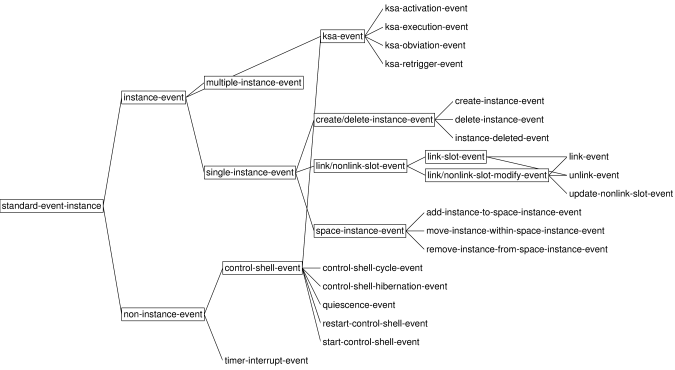
\includegraphics[scale=0.85]{agenda-shell-events}
\end{center}
\W\end{iftex}

\noindent Event classes shown within rectangles are abstract event classes
that cannot be signaled.  Nevertheless, abstract event classes are
very convenient if we wish to attach an event function to an entire
subtree of event classes.  We used abstract event classes to advantage
earlier when we enabled display of all control-shell events by
evaluating:
%
\begin{example}\color{darkergray}%
  gbbopen-user> (enable-event-printing '(control-shell-event :plus-subevents))
  nil
  gbbopen-user>
\end{example}


Add the following form at the end of your \code{tutorial-example.lisp} file:
%
\begin{example}
(add-event-function 'initializations 'start-control-shell-event
                    ;; Initializations should be done first!
                    :priority 100)
\end{example}

(We'll place the \textbf{add-event-function} form immediately after the
\code{initializations} function definition in our file, but this choice of
location is purely a code organizational style preference---the form could be
placed anywhere relative to the function definition.)

\subsection*{Step 3: Run the application}

\bfindex{start-control-shell}%
Start a fresh Common Lisp session, compile and load the
\code{tutorial-example.lisp} file directly from the editor buffer (using
\code{C-c C-k} in SLIME; \code{C-c C-b} in ELI) and start the Agenda Shell
again:
%
\begin{example}\color{darkergray}%
  gbbopen-user> \textcolor{black}{(start-control-shell)}
  ;; Control shell 1 started
  ;; No executable KSAs remain, exiting control shell
  ;; Control shell 1 exited: 3 cycles completed
  ;; Run time: 0 seconds
  ;; Elapsed time: 0 seconds
  :quiescence
  gbbopen-user>
\end{example}

Note that our developing application performs the same as it did in the last
exercise, but now our \code{initializations} event function is taking care of
all the details of starting up our application.  We no longer have to remember
to create the \code{known-world} space instance or to delete the blackboard
repository before running the application another time.

\subsection*{Step 4: Run it Again}

\bfindex{start-control-shell}%
Let's verify that we can re-run our application. Without doing anything else,
start the Agenda Shell again:
%
\begin{example}\color{darkergray}%
  gbbopen-user> \textcolor{black}{(start-control-shell)}
  ;; Control shell 1 started
  ;; No executable KSAs remain, exiting control shell
  ;; Control shell 1 exited: 3 cycles completed
  ;; Run time: 0 seconds
  ;; Elapsed time: 0 seconds
  :quiescence
  gbbopen-user>
\end{example}

As before our \code{initializations} event function took care of all the
details of starting up our application.

\subsection*{Step 5: It's a new world$\ldots$}

\bfindexit{make-space-instance}%
GBBopen allows us to restrict the classes of unit instances that can be stored
on a space instance.  For example, we can limit the \code{known-world} to
\code{location} unit instances by specifying an \code{:allowed-unit-classes}
value to \code{make-space-instance}:
%
\begin{example}\color{darkergray}%
  (defun initializations (event-name &key &allow-other-keys)
    (declare (ignore event-name))
    ;; Clean up any previous run:
    (delete-blackboard-repository)
    ;; Make a new known-world space instance:
    (make-space-instance 
     '(known-world)
     :dimensions '((x :ordered) (y :ordered))
     \textcolor{black}{:allowed-unit-classes 'location}))
\end{example}
%
Attempting to add any unit-instance that is not a \code{location} to
\code{known-world} will now generate an error.

It is often convenient to specify the dimensions of a space-instance relative
to those of one or more unit classes.  Edit the definition of
\code{initializations}, removing the \code{x} and \code{y} dimensions
specification:
%
\begin{example}\color{darkergray}%
(defun initializations (event-name &key &allow-other-keys)
  (declare (ignore event-name))
  ;; Clean up any previous run:
  (delete-blackboard-repository)
  ;; Make a new known-world space instance:
  (make-space-instance 
   '(known-world)
   :dimensions \textcolor{red}{'((x :ordered) (y :ordered))}
   :allowed-unit-classes 'location))
\end{example}
%
and replacing it with a call of \textbf{dimensions-of} to
obtain the dimensions associated with instances of the \code{location}
unit class:
%
\begin{example}\color{darkergray}%
(defun initializations (event-name &key &allow-other-keys)
  (declare (ignore event-name))
  ;; Clean up any previous run:
  (delete-blackboard-repository)
  ;; Make a new known-world space instance:
  (make-space-instance 
   '(known-world)
   :dimensions \textcolor{black}{(dimensions-of 'location)}
   :allowed-unit-classes 'location))
\end{example}

\subsection*{Step 6: Run the application again}

Compile and load the \code{tutorial-example.lisp} file directly from the
editor buffer (using \code{C-c C-k} in SLIME; \code{C-c C-b} in ELI) and start
the Agenda Shell again:
%
\begin{example}\color{darkergray}%
  gbbopen-user> \textcolor{black}{(start-control-shell)}
  ;; Control shell 1 started
  ;; No executable KSAs remain, exiting control shell
  ;; Control shell 1 exited: 3 cycles completed
  ;; Run time: 0 seconds
  ;; Elapsed time: 0 seconds
  :quiescence
  gbbopen-user>
\end{example}

\bfindexit{describe-space-instance}%
Verify the dimensionality of the \code{known-world} space instance by evaluating:
%
\begin{example}\color{darkergray}%
  gbbopen-user> \textcolor{black}{(describe-space-instance '(known-world))}
  Standard-space-instance #<standard-space-instance (known-world)>
    Allowed unit classes: t
    Dimensions:
      (x :ordered)
      (y :ordered)
  gbbopen-user>
\end{example}

%% ========================================================================
%%  Define Another KS

\T\markright{}%
\T\pagestyle{plain}
\T\cleardoublepage
\W\xname{tutorial-another-ks}
\T\pagestyle{fancy}
\T\thispagestyle{fancybottom}
\T\renewcommand{\headrulewidth}{0pt}
\section{Add Another KS}
\label{sec:another-ks}%

The last exercise made it easy to initialize and run our application
repeatedly by simply starting the Agenda Shell.  We also specified the
dimensionality of our \code{known-world} space instance relative to the
dimensional specifications of the \code{location} unit class.  With these
niceties in place, its time to move beyond our initial \code{location} unit
instance.

\fndocrule

This exercise shows you how to:
\begin{tightitemize}
\item Add an additional dimension to a unit class
\item Define a KS that obtains its execution-context information from its
  triggering unit instance
\item Extend the random-walk application to do some walking
\item Explore the resulting random walk
\end{tightitemize}

\fndocrule

\subsection*{Prerequisites}

\begin{tightitemize}
\item The \code{tutorial-example.lisp} file as modified thus far:
\end{tightitemize}

\begin{example}
(in-package :gbbopen-user)

(define-unit-class location ()
  (x y)
  (:dimensional-values
    (x :point x)
    (y :point y))
  (:initial-space-instances (known-world)))

(defmethod print-instance-slots ((location location) stream)
  (call-next-method)
  (when (and (slot-boundp location 'x)
             (slot-boundp location 'y))
    (format stream " (~s ~s)"
            (x-of location)
            (y-of location))))

;;; ======================================================================
;;;   Startup KS

(defun startup-ks-function (ksa)
  (declare (ignore ksa))
  ;; Create an initial location unit instance at (0,0):
  (make-instance 'location :x 0 :y 0))

(define-ks startup-ks
    :trigger-events ((start-control-shell-event))
    :execution-function 'startup-ks-function)

;;; ======================================================================
;;;   Initializations (run at Agenda Shell startup)

(defun initializations (event-name &key &allow-other-keys)
  (declare (ignore event-name))
  ;; Clean up any previous run:
  (delete-blackboard-repository)
  ;; Make a new known-world space instance:
  (make-space-instance 
   '(known-world)
   :dimensions (dimensions-of 'location)))

(add-event-function 'initializations 'start-control-shell-event
                    ;; Initializations should be done first!
                    :priority 100)
\end{example}

\begin{tightitemize}
\item The \code{:agenda-shell-user} module is loaded
\end{tightitemize}

\subsection*{Step 1: Add  another dimension}

It's time we introduce the notion of time to our application.  Edit the
\code{location} unit-class definition in \code{tutorial-example.lisp}, adding
a new slot, \code{time}, to the \code{location} unit class definition and a
corresponding \code{time} dimensional value:
%
\begin{example}\color{darkergray}%
(define-unit-class location ()
  (\textcolor{black}{time} 
   x y)
  (:dimensional-values
    \textcolor{black}{(time :point time)}
    (x :point x)
    (y :point y))
  (:initial-space-instances (known-world)))
\end{example}

Recall that we specified that the dimensions of the \code{known-world} space
instance that is created by our \code{initializations} function relative to
the dimensions of the \code{location} unit class:
%
\begin{example}\color{darkergray}%
  (make-space-instance 
      '(known-world)
      :dimensions (dimensions-of 'location)))
\end{example}
%
Therefore, we don't need to modify our call to \code{make-space-instance} in
order to add \code{time} as a dimension of \code{known-world}.

Next, modify \code{startup-ks-function} in \code{tutorial-example.lisp} so
that it creates the initial \code{location} unit instance at time 0:
%
\begin{example}\color{darkergray}%
(defun startup-ks-function (ksa)
  (declare (ignore ksa))
  ;; Create an initial location unit instance at (0,0) \textcolor{black}{at time 0}:
  (make-instance 'location \textcolor{black}{:time 0} :x 0 :y 0))
\end{example}

\subsection*{Step 2: A test of time}

Let's check our work.  Compile and load the
\code{tutorial-example.lisp} file directly from the editor buffer (using
\code{C-c C-k} in SLIME; \code{C-c C-b} in ELI) and start the Agenda Shell
again:
%
\begin{example}\color{darkergray}%
  gbbopen-user> \textcolor{black}{(start-control-shell)}
  ;; Control shell 1 started
  ;; No executable KSAs remain, exiting control shell
  ;; Control shell 1 exited: 3 cycles completed
  ;; Run time: 0 seconds
  ;; Elapsed time: 0 seconds
  :quiescence
  gbbopen-user>
\end{example}

\bfindexit{describe-instance}%
\bfindexit{find-instance-by-name}%
Check that the initial \code{location} unit instance is at \code{time} zero:
%
\begin{example}\color{darkergray}%
  gbbopen-user> \textcolor{black}{(describe-instance (find-instance-by-name 1 'location))}
  Location #<location 1 (0 0)>
    Instance name: 1
    Space instances: ((known-world))
    Dimensional values:
      time:  0
      x:  40
      y:  60
    Non-link slots:
      time:  0
      x:  40
      y : 60
    Link slots: None
  gbbopen-user>
\end{example}

\subsection*{Step 3: Define another KS}

Define a KS called \code{random-walk-ks} that:

\begin{tightitemize}
\item Is triggered when a \code{location} unit instance is created
\item Has a constant KSA rating of 100
\item Has an execution function called \code{random-walk-ks-function}, which:
\begin{tightitemize}
\item Checks if we've already walked for 75 locations and prints a message if
  we have. 
\item Otherwise:
\begin{tightitemize}
\item Determines a random location for which the x and y values are within 10
  of the x and y values of the triggering unit instance (that is, the
  \code{location} instance whose creation triggered the \code{random-walk-ks}
  KS)
\item If both of the x and y values for the new random location are between
  -50 and 50, creates a \code{location} unit instance at the random location;
  otherwise, prints a message indicating that we've walked off the world
\end{tightitemize}
\end{tightitemize}
\end{tightitemize}

\subsubsection*{Step 3a: Define a utility function}

Begin implementing the \code{random-walk-ks} by adding the following
utility function to the end of your \code{tutorial-example.lisp} file:

\begin{example}
;;; ======================================================================
;;;   Random-walk KS

(defun add-linear-variance (value max-variance)
  ;;; Returns a new random value in the interval
  ;;; [(- value max-variance), (+ value max-variance)]
  (+ value (- (random (1+ (* max-variance 2))) max-variance)))
\end{example}

Then compile the definition (using \code{C-c C-c} in SLIME or \code{C-c
  C-x} in ELI) and evaluate the following test in the REPL:

\bfindex{printv}%
\begin{example}\color{darkergray}%
  gbbopen-user> \textcolor{black}{(dotimes (i 15) (printv (add-linear-variance 0 10)))}
  ;;  (add-linear-variance 0 10) => 8
  ;;  (add-linear-variance 0 10) => 9
  ;;  (add-linear-variance 0 10) => 4
  ;;  (add-linear-variance 0 10) => 3
  ;;  (add-linear-variance 0 10) => -4
  ;;  (add-linear-variance 0 10) => -10
  ;;  (add-linear-variance 0 10) => -1
  ;;  (add-linear-variance 0 10) => 0
  ;;  (add-linear-variance 0 10) => 4
  ;;  (add-linear-variance 0 10) => 5
  ;;  (add-linear-variance 0 10) => 8
  ;;  (add-linear-variance 0 10) => -5
  ;;  (add-linear-variance 0 10) => -3
  ;;  (add-linear-variance 0 10) => 7
  ;;  (add-linear-variance 0 10) => 6
  nil
  gbbopen-user>
\end{example}

Because \code{add-linear-variance} is stochastic, your results will be
similar but not identical.  Note that we used GBBopen's \textbf{printv}
macro to display the result of each generated value.  \textbf{Printv} can
greatly assist debugging by printing forms and the results of evaluating
them.  \textbf{Printv} can be transparently wrapped around any form in a
complex function definition, as it evaluates and displays all the forms in
its body and returns the values resulting from evaluating the last form:

\begin{example}\color{darkergray}%
  gbbopen-user>  (printv "Some multiple values" (values 1 2) "Some more" (values 3 4 5))
  ;; Some multiple values
  ;;  (values 1 2) => 1; 2
  ;; Some more
  ;;  (values 3 4 5) => 3; 4; 5
  4
  5
  6
  gbbopen-user>
\end{example}

\subsubsection*{Step 3b: Define the \code{random-walk-ks} execution function}

Next add the following KS-execution function to the end of your
\code{tutorial-example.lisp} file:

\begin{example}
(defun random-walk-ks-function (ksa)
  ;;; Move to the next (random) location in the world
  (let* ((trigger-instance (sole-trigger-instance-of ksa))
         ;; The new time is one greater than the stimulus instance's time:
         (time (1+ (time-of trigger-instance))))
    (cond
     ;; If the maximum time value (75) is reached, tell the user we've
     ;; walked too long:
     ((>= time 75) (format t "~2&Walked too long.~\%"))
     (t ;; The new location is +/- 10 of the stimulus instance's location:
      (let ((x (add-linear-variance (x-of trigger-instance) 10))
            (y (add-linear-variance (y-of trigger-instance) 10)))
        (cond
         ;; Check that the new location is within the known-world
         ;; boundaries.  If so, create the new location instance:
         ((and (<= -50 x 50) (<= -50 y 50))
          (make-instance 'location 
            :time time 
            :x x 
            :y y))
         ;; Otherwise, tell the user that we've walked too far away:
         (t (format t "~2\&Walked off the world: (~d, ~d).~\%" x y))))))))
\end{example}

\bfindex{sole-trigger-instance-of}%
Unlike the KS-execution functions that we have defined previously,
\code{random-walk-ks-function} does not ignore its \code{ksa} argument.
Instead, it calls \textbf{sole-trigger-instance-of} with the \code{ksa}
unit-instance argument in order to obtain the \code{location} unit instance
whose creation triggered the KSA.  This pattern of obtaining the unit instance
that triggered a KSA and then using that triggering unit instance as the
context for the KS execution is typical of many KSs. 

\subsubsection*{Step 3c: Add the \code{random-walk-ks} definition}

Finally, add this \code{define-ks} form to the end of your
\code{tutorial-example.lisp} file to complete the \code{random-walk-ks}
definition:

\bfindexit{define-ks}%
\codeindex{quiescence-event}%
\begin{example}
(define-ks random-walk-ks
   :trigger-events ((create-instance-event location))
   :rating 100
   :execution-function 'random-walk-ks-function)
\end{example}

\subsection*{Step 4:  Run the application}

\bfindexit{start-control-shell}%
Compile and load the \code{random-walk-ks} forms, and then start the Agenda Shell:
%
\begin{example}\color{darkergray}%
  gbbopen-user> \textcolor{black}{(start-control-shell)}
  ;; Control shell 1 started

  Walked off the world: (23, 55).
  ;; No executable KSAs remain, exiting control shell
  ;; Control shell 1 exited: 64 cycles completed
  ;; Run time: 0.01 seconds
  ;; Elapsed time: 0 seconds
  :quiescence
  gbbopen-user>
\end{example}

\bfindexit{:dsbb}%
It looks like something happened! (Again, because \code{add-linear-variance}
is stochastic, your results will be similar but not identical.)  Let's look at
the blackboard repository and see how many \code{location} unit instances were
created:
%
\begin{example}\color{darkergray}%
  gbbopen-user> \textcolor{black}{:dsbb}

  Space Instance                Contents
  --------------                --------
  known-world                   61 instances (61 location)

  Unit Class                    Instances
  ----------                    ---------
  control-shell                         1 *
  ks                                    1 +
  ksa-queue                             2 +
  location                             61
  ordered-ksa-queue                     1 +
  standard-space-instance               1
                                ---------
                                       67 instances
  gbbopen-user>
\end{example}

The 61 \code{location} instances makes sense.  Previously, it required 3
control-shell cycles to create the initial \code{location} unit instance (one
to execute the \code{initial-ks} KSA followed by two additional cycles of
quiescence before the Agenda Shell exits).  We now create one additional
\code{location} unit instance with every execution of \code{random-walk-ks},
so we always create 3 fewer \code{location} instances than the total
number of control-shell cycles.

\subsection*{Step 5:  Where have we been?}

\bfindexit{map-instances-of-class}%
It would be interesting to see where our random walk has taken us.  We could
use GBBopen's \textbf{map-instances-of-class} iterator to print each of the
\code{location} unit instances:
%
\begin{example}\color{darkergray}%
  gbbopen-user> \textcolor{black}{(map-instances-of-class #'print 'location)}

  #<location 58 (5 31)> 
  #<location 13 (-7 10)> 
  #<location 26 (-40 35)> 
  #<location 39 (-4 3)> 
  #<location 52 (2 23)> 
  #<location 7 (3 17)> 
  #<location 20 (2 27)> 
  #<location 33 (-25 6)> 
  #<location 46 (-2 32)> 
       ...
  #<location 31 (-22 18)> 
  #<location 44 (-7 14)> 
  #<location 57 (2 41)> 
  #<location 12 (-15 15)> 
  #<location 25 (-32 38)> 
  #<location 38 (-10 -4)> 
  #<location 51 (-2 16)> 
  #<location 6 (10 27)> 
  #<location 19 (-1 17)> 
  #<location 32 (-25 12)> 
  #<location 45 (-7 23)> 
  nil
  gbbopen-user>
\end{example}
%
Unfortunately, the order that unit instances are supplied to the \code{print}
function is not controllable.  Our walk would be much clearer if we printed
the \code{location}s in time order.

\bfindexit{map-sorted-instances-of-class}%
We might consider taking advantage of the instance names that GBBopen assigns
to unit instances.  We could do something like the following:
%
\begin{example}\color{darkergray}%
  gbbopen-user> \textcolor{red}{(dotimes (i 76)
                  (let ((location (find-instance-by-name i 'location)))
                    (when location
                       (print location))))}

  #<location 1 (0 0)> 
  #<location 2 (10 4)> 
  #<location 3 (19 10)> 
  #<location 4 (14 9)> 
  #<location 5 (14 18)> 
  #<location 6 (10 27)> 
  #<location 7 (3 17)> 
  #<location 8 (-6 20)> 
  #<location 9 (4 15)> 
  #<location 10 (-5 14)> 
       ...
  #<location 50 (5 26)> 
  #<location 51 (-2 16)> 
  #<location 52 (2 23)> 
  #<location 53 (9 33)> 
  #<location 54 (7 43)> 
  #<location 55 (-2 36)> 
  #<location 56 (0 46)> 
  #<location 57 (2 41)> 
  #<location 58 (5 31)> 
  #<location 59 (13 39)> 
  #<location 60 (17 41)> 
  #<location 61 (21 50)> 
  nil
  gbbopen-user>
\end{example}

This is a bad idea for several reasons.  First, we are looking up every
\code{location} unit instance by its instance name, which is less efficient
than operating on \code{location} instances directly.  While this isn't an
significant issue in expressions that we evaluate in the REPL to investigate
our application, we should seek to avoid such inefficiencies in application
code.  More importantly, however, the \code{location} instance name just
happens to mirror the sequencing that we really want to display---the
\code{time} value of the \code{location}s.  We should find a way to sequence
\code{location} printing that relies on the \code{time} values directly.

\bfindex{map-sorted-instances-of-class}%
GBBopen provides a variant of \textbf{map-instances-of-class}, called
\textbf{map-sorted-instances-of-class}, that sorts the unit instances based on
a comparison predicate and an optional \code{:key} accessor function that
suits our needs:
%
\begin{example}\color{darkergray}%
  gbbopen-user> \textcolor{black}{(map-sorted-instances-of-class #'print 'location #'< 
                   :key #'time-of)}

  #<location 1 (0 0)> 
  #<location 2 (10 4)> 
  #<location 3 (19 10)> 
  #<location 4 (14 9)> 
  #<location 5 (14 18)> 
  #<location 6 (10 27)> 
  #<location 7 (3 17)> 
  #<location 8 (-6 20)> 
  #<location 9 (4 15)> 
  #<location 10 (-5 14)> 
       ...
  #<location 50 (5 26)> 
  #<location 51 (-2 16)> 
  #<location 52 (2 23)> 
  #<location 53 (9 33)> 
  #<location 54 (7 43)> 
  #<location 55 (-2 36)> 
  #<location 56 (0 46)> 
  #<location 57 (2 41)> 
  #<location 58 (5 31)> 
  #<location 59 (13 39)> 
  #<location 60 (17 41)> 
  #<location 61 (21 50)> 
  nil
  gbbopen-user>
\end{example}

\bfindex{do-sorted-instances-of-class}%
Using \textbf{map-sorted-instances-of-class} involves a sorting operation, so
this approach still has some efficiency concerns for use in application code.
However, it suits our REPL-exploration needs just fine.  (There is a
\textbf{do-sorted-instances-of-class} macro, if an iterative style is
preferred over a mapper.)  We will explore a more efficient approach to
displaying the random walk in the next exercise.

\subsection*{Step 6:  Run the application a few more times}

\bfindexit{start-control-shell}%
If we run the application a few more times, we eventually encounter a case
where we create the allotted 75 \code{location} unit instances without walking
off the \code{known-world}:
%
\begin{example}\color{darkergray}%
  gbbopen-user> \textcolor{black}{(start-control-shell)}
  ;; Control shell 1 started

  Walked too long.
  ;; No executable KSAs remain, exiting control shell
  ;; Control shell 1 exited: 78 cycles completed
  ;; Run time: 0.04 seconds
  ;; Elapsed time: 0 seconds
  :quiescence
  gbbopen-user>
\end{example}

\bfindexit{map-sorted-instances-of-class}%
Here is one such random walk:
%
\begin{example}\color{darkergray}%
  gbbopen-user> \textcolor{black}{(map-sorted-instances-of-class #'print 'location #'< 
                   :key #'time-of)}

  #<location 1 (0 0)> 
  #<location 2 (2 7)> 
  #<location 3 (-1 5)> 
  #<location 4 (-1 0)> 
  #<location 5 (3 -2)> 
  #<location 6 (13 -7)> 
  #<location 7 (8 -5)> 
  #<location 8 (1 2)> 
  #<location 9 (8 0)> 
  #<location 10 (5 8)> 
       ...
  #<location 70 (-13 -11)> 
  #<location 71 (-13 -6)> 
  #<location 72 (-9 -6)> 
  #<location 73 (1 -4)> 
  #<location 74 (-8 -11)> 
  #<location 75 (-13 -15)> 
  nil
  gbbopen-user>
\end{example}

%% ========================================================================
%%  Making Connections

\T\markright{}%
\T\pagestyle{plain}
\T\cleardoublepage
\W\xname{tutorial-connections}
\T\pagestyle{fancy}
\T\thispagestyle{fancybottom}
\T\renewcommand{\headrulewidth}{0pt}
\section{Making Connections}
\label{sec:connections}%

%\begin{center}
%\textcolor{caution}{[Construction ahead...]}
%\end{center}

We finally did some walking in the last exercise and learned how to display
the \code{location}s in our walk from the REPL.  In this exercise, we learn
how to use GBBopen's link capabilities to represent relationships among unit
instances.  Links are an important aspect of almost every GBBopen application,
so it's time that we started taking advantage of them.

\fndocrule

This exercise shows you how to:
\begin{tightitemize}
\item Add link slots to a unit class
\item Use link slots to traverse and display the resulting random walk
\end{tightitemize}

\fndocrule

\subsection*{Prerequisites}

\begin{tightitemize}
\item The \code{tutorial-example.lisp} file as modified thus far:
\end{tightitemize}

\begin{example}
(in-package :gbbopen-user)

(define-unit-class location ()
  (time 
   x y)
  (:dimensional-values
    (time :point time)
    (x :point x)
    (y :point y))
  (:initial-space-instances (known-world)))

(defmethod print-instance-slots ((location location) stream)
  (call-next-method)
  (when (and (slot-boundp location 'x)
             (slot-boundp location 'y))
    (format stream " (~s ~s)"
            (x-of location)
            (y-of location))))

;;; ======================================================================
;;;   Startup KS

(defun startup-ks-function (ksa)
  (declare (ignore ksa))
  ;; Create an initial location unit instance at (0,0):
  (make-instance 'location :time 0 :x 0 :y 0))

(define-ks startup-ks
    :trigger-events ((start-control-shell-event))
    :execution-function 'startup-ks-function)

;;; ======================================================================
;;;   Initializations (run at Agenda Shell startup)

(defun initializations (event-name &key &allow-other-keys)
  (declare (ignore event-name))
  ;; Clean up any previous run:
  (delete-blackboard-repository)
  ;; Make a new known-world space instance:
  (make-space-instance 
   '(known-world)
   :dimensions (dimensions-of 'location)))

(add-event-function 'initializations 'start-control-shell-event
                    ;; Initializations should be done first!
                    :priority 100)

;;; ======================================================================
;;;   Random-walk KS

(defun add-linear-variance (value max-variance)
  ;;; Returns a new random value in the interval
  ;;; [(- value max-variance), (+ value max-variance)]
  (+ value (- (random (1+ (* max-variance 2))) max-variance)))

(defun random-walk-ks-function (ksa)
  ;;; Move to the next (random) location in the world
  (let* ((trigger-instance (sole-trigger-instance-of ksa))
         ;; The new time is one greater than the stimulus instance's time:
         (time (1+ (time-of trigger-instance))))
    (cond
     ;; If the maximum time value (75) is reached, tell the user we've
     ;; walked too long:
     ((>= time 75) (format t "~2&Walked too long.~\%"))
     (t ;; The new location is +/- 10 of the stimulus instance's location:
      (let ((x (add-linear-variance (x-of trigger-instance) 10))
            (y (add-linear-variance (y-of trigger-instance) 10)))
        (cond
         ;; Check that the new location is within the known-world
         ;; boundaries.  If so, create the new location instance:
         ((and (<= -50 x 50) (<= -50 y 50))
          (make-instance 'location 
            :time time 
            :x x 
            :y y))
         ;; Otherwise, tell the user that we've walked too far away:
         (t (format t "~2&Walked off the world: (~d, ~d).~\%" x y))))))))

(define-ks random-walk-ks
    :trigger-events ((create-instance-event location))
    :rating 100
    :execution-function 'random-walk-ks-function)
\end{example}

\begin{tightitemize}
\item The \code{:agenda-shell-user} module is loaded
\end{tightitemize}

\subsection*{Step 1: Add  a link}

In the last exercise, we used \textbf{map-sorted-instances-of-class} to
display the random walk.  Another way that we could represent the walk is by
connect each newly created \code{location} unit instance to the
\code{location} unit instance that preceded it in the walk.  We'll use
GBBopen's link capabilities to do this.

A \textit{link} is a bidirectional relationship between two unit instances
that is implemented by two pointers. From the perspective of a particular unit
instance, each link consists of an outgoing, or \textit{direct}, pointer to
another unit instance and an incoming, or \textit{inverse}, pointer that is
stored in unit instance pointed to by the direct pointer.  GBBopen
automatically maintains the bidirectional-link consistency of these pointers
when creating new links, deleting existing links, or deleting unit instances.
Links remove the possibility of ``one-sided'' relationships or ``dangling''
pointers to deleted unit instances.

Edit the \code{location} unit-class definition in your
\code{tutorial-example.lisp} file, adding two link slots, \code{next-location}
and \code{previous-location}, to the \code{location} unit class definition:
%
\begin{example}\color{darkergray}%
(define-unit-class location ()
  (time 
   x y
   \textcolor{black}{(next-location
    :link (location previous-location :singular t) 
    :singular t)
   (previous-location
    :link (location next-location :singular t)  
    :singular t)})
  (:dimensional-values
    (time :point time)
    (x :point x)
    (y :point y))
  (:initial-space-instances (known-world)))
\end{example}

Each link-slot specification is a list whose first element is the name of the
link slot.  This is followed by the link slot option \code{:link} and a
concise specification of the inverse link slot associated with that link slot.
In this case, the \code{next-location}/\code{previous-location} link is
between instances of the same (\code{location}) unit class, but often links
are between instances of different unit classes. 

Links can be many-to-many, many-to-one, one-to-many, or one-to-one.  In this
case, the \code{next-location}/\code{previous-location} link is one-to-one,
which is specified by including the \code{:singular t} slot option in the
link-slot definition (and the corresponding \code{:singular t} specification
in the concise inverse-link-slot specification).  To help clarify the
specification of link slot arity, let's temporarily assume that we want a
\code{location} instance that can have many next locations, but only a single
previous location.  This link relation would be specified as follows:
%
\begin{example}\color{darkergray}%
    ...
 \textcolor{blue}{(next-locations
  :link (location previous-location :singular t)))
 (previous-location
  :link (location next-locations)  
  :singular t)}
    ...
\end{example}

We've followed the natural GBBopen convention of giving singular link
slots a singular name (such as \code{previous-location}) and link
slots that can contain multiple links a plural name (such as
\code{next-locations}).  Note that the \code{:singular} option is
associated with the \code{previous-location} link slot as both a slot
option in the \code{previous-location} link-slot definition and in the
concise inverse-link-slot specification for \code{previous-location}
in the \code{next-locations} link-slot definition.

\subsection*{Step 2: Break some links}

The concise inverse-link-slot specification supplied by the
\code{:link} slot option provides a ``double entry'' redundancy that
is useful when links are between instances of different unit classes,
as the link can be understood by viewing either class definition.  The
redundancy also helps GBBopen recognize inconsistencies in link
specifications.  The function \textbf{check-link-consistency} asks
GBBopen to validate that all link definitions are consistent.  Let's
try it on our current random-walk application.  Compile and load the
latest changes in your \code{tutorial-example.lisp} file (including
the new \code{next-location} and \code{previous-location} link slots).
Then check link consistency:
%
\begin{example}\color{darkergray}%
  gbbopen-user> \textcolor{black}{(check-link-consistency)}
  ;; All link definitions are consistent.
  t
  gbbopen-user>
\end{example}
%
GBBopen reports that all link definitions are consistent.

Suppose that we had forgotten to add the \code{previous-location} end
of the link in our \code{location} unit-class definition. Edit the
\code{location} unit-class definition in your
\code{tutorial-example.lisp} file, adding the line \code{\#+ignore}
immediately before the \code{previous-location} link-slot definition:
%
\begin{example}\color{darkergray}%
(define-unit-class location ()
  (time 
   x y
   (next-location
    :link (location previous-location :singular t) 
    :singular t)
    \textcolor{black}{\#+ignore}     
   (previous-location
    :link (location next-location :singular t)  
    :singular t))
  (:dimensional-values
    (time :point time)
    (x :point x)
    (y :point y))
  (:initial-space-instances (known-world)))
\end{example}

The \code{\#+ignore} read-time conditionalization tells Common Lisp to
skip over the next form if \code{ignore} is not an element of the
feature list \code{*features*}.  By convention, \code{ignore} is never
added to \code{*features*}, so \code{\#+ignore} is a handy mechanism
for temporarily ``commenting out'' a single form.

Compile the now-defective definition (using \code{C-c C-c} in SLIME or
\code{C-c C-x} in ELI) and then recheck link consistency:
%
\begin{example}\color{darkergray}%
  gbbopen-user> \textcolor{black}{(check-link-consistency)}
  Warning: The inverse of link slot next-location in unit class location 
           refers to link slot previous-location which is not present in 
           unit class location.
  nil
  gbbopen-user>
\end{example}
%
As expected, GBBopen alerts us to the problem.

Remove the \code{\#+ignore} that we just added and comment out the
\code{:singular t} portion of the inverse link-slot specification in 
\code{next-location}:
%
\begin{example}\color{darkergray}%
(define-unit-class location ()
  (time 
   x y
   (next-location
    :link (location previous-location\textcolor{black}{) ;} :singular t) 
    :singular t)
    \textcolor{red}{#+ignore}     
   (previous-location
    :link (location next-location :singular t)  
    :singular t))
  (:dimensional-values
    (time :point time)
    (x :point x)
    (y :point y))
  (:initial-space-instances (known-world)))
\end{example}

Compile the again-defective definition (using \code{C-c C-c} in SLIME or
\code{C-c C-x} in ELI) and then recheck link consistency:
%
\begin{example}\color{darkergray}%
  gbbopen-user> \textcolor{black}{(check-link-consistency)}
  Warning: Link slot next-location in unit class location incorrectly 
           declares its inverse link slot previous-location in unit 
           class location as not singular.
  nil
  gbbopen-user>
\end{example}
%
Once again, GBBopen has alerted us to the problem.

Restore the \code{:singular t} portion of the inverse link-slot
specification in \code{next-location} that we just commented out:
%
\begin{example}\color{darkergray}%
(define-unit-class location ()
  (time 
   x y
   (next-location
    :link (location previous-location\textcolor{red}{) ;} :singular t) 
    :singular t)
   (previous-location
    :link (location next-location :singular t)  
    :singular t))
  (:dimensional-values
    (time :point time)
    (x :point x)
    (y :point y))
  (:initial-space-instances (known-world)))
\end{example}

Then recompile and recheck link consistency:
%
\begin{example}\color{darkergray}%
  gbbopen-user> \textcolor{black}{(check-link-consistency)}
  ;; All link definitions are consistent.
  t
  gbbopen-user>
\end{example}

\subsection*{Step 3: Create some links}

Let's use our newly defined \code{next-location}/\code{previous-location} link
to connect our \code{location} unit instances.  Edit the
\code{random-walk-ks-function} definition in your \code{tutorial-example.lisp}
file, adding the trigger instance as a new \code{:previous-location} argument
to \code{make-instance}:
%
\begin{example}\color{darkergray}%
(defun random-walk-ks-function (ksa)
  ;;; Move to the next (random) location in the world
  (let* ((trigger-instance (sole-trigger-instance-of ksa))
         ;; The new time is one greater than the stimulus instance's time:
         (time (1+ (time-of trigger-instance))))
    (cond
     ;; If the maximum time value (75) is reached, tell the user we've
     ;; walked too long:
     ((>= time 75) (format t "~2&Walked too long.~\%"))
     (t ;; The new location is +/- 10 of the stimulus instance's location:
      (let ((x (add-linear-variance (x-of trigger-instance) 10))
            (y (add-linear-variance (y-of trigger-instance) 10)))
        (cond
         ;; Check that the new location is within the known-world
         ;; boundaries.  If so, create the new location instance:
         ((and (<= -50 x 50) (<= -50 y 50))
          (make-instance 'location 
            :time time 
            :x x 
            :y y
            \textcolor{black}{:previous-location trigger-instance}))
         ;; Otherwise, tell the user that we've walked too far away:
         (t (format t "~2&Walked off the world: (~d, ~d).~\%" x y))))))))
\end{example}

Compile the \code{random-walk-ks-function} (using \code{C-c C-c} in SLIME or
\code{C-c C-x} in ELI) and then run the application:
%
\begin{example}\color{darkergray}%
  gbbopen-user> \textcolor{black}{(start-control-shell)}
  ;; Control shell 1 started

  Walked off the world: (55, 35).
  ;; No executable KSAs remain, exiting control shell
  ;; Control shell 1 exited: 66 cycles completed
  ;; Run time: 0.01 seconds
  ;; Elapsed time: 0 seconds
  :quiescence
  gbbopen-user>
\end{example}

Let's describe a couple of \code{location} unit instances to check our work.
First, the initial \code{location} unit instance:
%
\begin{example}\color{darkergray}%
  gbbopen-user> \textcolor{black}{(describe-instance (find-instance-by-name 1 'location))}
  Location #<location 1 (0 0)>
    Instance name: 1
    Space instances: ((known-world))
    Dimensional values:
      time:  0
      x:  40
      y:  60
    Non-link slots:
      time:  0
      x:  40
      y:  60
    Link slots:
      next-location:  #<location 2 (-10 10)>
      previous-location:  nil
  gbbopen-user>
\end{example}

Note that the \code{next-location} link slot points to the next
\code{location} unit instance in our random walk.  Let's describe that
unit instance:
%
\begin{example}\color{darkergray}%
  gbbopen-user> \textcolor{black}{(describe-instance (find-instance-by-name 2 'location))}
  Location #<location 2 (-10 10)>
    Instance name: 2
    Space instances: ((known-world))
    Dimensional values:
      time:  1
      x:  -10
      y:  10
    Non-link slots:
      time:  1
      x:  -10
      y:  10
    Link slots:
      next-location:  #<location 3 (-6 19)>
      previous-location:  #<location 1 (0 0)>
  gbbopen-user>
\end{example}

Its \code{next-location} link slot points to the third \code{location} unit
instance in our random walk and its \code{previous-location} link slot points
back to the initial \code{location} unit instance.

We can now follow the links to display the random walk:
%
\begin{example}\color{darkergray}%
  gbbopen-user> \textcolor{black}{(loop with location = (find-instance-by-name 1 'location) 
                  do (print location)
                  while (setf location (next-location-of location)))}

  #<location 1 (0 0)> 
  #<location 2 (-10 10)> 
  #<location 3 (-6 19)> 
  #<location 4 (0 14)> 
  #<location 5 (-1 14)> 
  #<location 6 (8 10)> 
  #<location 7 (17 3)> 
  #<location 8 (7 -6)> 
  #<location 9 (10 4)> 
  #<location 10 (5 -5)> 
       ...
  #<location 60 (29 17)> 
  #<location 61 (31 21)> 
  #<location 62 (40 23)> 
  #<location 63 (45 28)> 
  nil
  gbbopen-user>
\end{example}

\subsection*{Step 4: Define a ``print walk'' KS}

\bfindexit{define-ks}%
\codeindex{:stop}%
\codeindex{quiescence-event}%
\bfindexit{find-instance-by-name}%
Let's add a new KS, \code{print-walk-ks}, that displays the random walk once
it is completed. Add the following KS to the end of your
\code{tutorial-example.lisp} file:
%
\begin{example}
;;; ======================================================================
;;;   Print-walk KS

(defun print-walk-ks-function (ksa)
  ;;; Starting with the initial location instance, print the instance name
  ;;; and location of the walk
    (declare (ignore ksa))
    (format t "~2\&The random walk:~\%")
      (let ((instance (find-instance-by-name 1 'location)))
      (while instance
        (format t "~s (~s ~s)~\%"
                (instance-name-of instance)
                (x-of instance)
                (y-of instance))
        (setf instance (next-location-of instance))))
    ;; Tell the Agenda Shell to exit:
    ':stop)

  (define-ks print-walk-ks
    :trigger-events ((quiescence-event))
    :rating 100
    :execution-function 'print-walk-ks-function)
\end{example}
%
The \code{print-walk-ks} is triggered by a \code{quiescence-event}.  Recall
that the Agenda Shell signals that quiescence has occurred when no
executable KSAs are available to be executed and then it continues for an
additional KS-execution cycle in case any executable KSAs resulted from the
quiescence event.  So, \code{print-walk-ks} will be triggered once no
\code{random-walk-ks} KSAs are triggered by newly created \code{location} unit
instances.

The \code{print-walk-ks-function} follows the
\code{next-location}/\code{previous-location} link to display the walk.  More
importantly, the function returns the keyword symbol \code{:stop}.  The Agenda
Shell checks the value returned by a KS execution function for this special
indicator and, if it is returned, the control shell is exited.  If we did not
return \code{:stop}, the \code{print-walk-ks} KS would be triggered and
activated on the first \code{quiescence-event}, the KSA would execute, then
the Agenda Shell would detect another quiescence condition, signal a new
\code{quiescence-event}, and our application would print the random walk over
and over again.

Let's compile our latest changes and then run our application with the new
\code{print-walk-ks} KS in place:
%
\begin{example}\color{darkergray}%
  gbbopen-user> \textcolor{black}{(start-control-shell)}
  ;; Control shell 1 started

  Walked off the world: (54, 15).

  The random walk:
  1 (0 0)
  2 (-6 9)
  3 (-14 8)
  4 (-5 6)
  5 (-13 5)
  6 (-11 13)
  7 (-11 4)
  8 (-17 8)
  9 (-21 15)
  10 (-12 14)
       ...
  35 (40 28)
  36 (50 22)
  37 (49 12)
  38 (47 10)
  ;; Explicit :stop issued by KS print-walk-ks
  ;; Control shell 1 exited: 41 cycles completed
  ;; Run time: 0.01 seconds
  ;; Elapsed time: 0 seconds
  :stop
  gbbopen-user>
\end{example}

%% ========================================================================
%%  Creating an Application

\T\markright{}%
\T\pagestyle{plain}
\T\cleardoublepage
\W\xname{tutorial-application}
\T\pagestyle{fancy}
\T\thispagestyle{fancybottom}
\T\renewcommand{\headrulewidth}{0pt}
\section{Creating a GBBopen Application}
\label{sec:application}%

GBBopen's \xreflink{Mini Module system}{sec:mini-module} provides facilities
that make it easy to define and use your own GBBopen applications.

\fndocrule

This exercise shows you how to:
\begin{tightitemize}
\item Structure an application using the \xreflink{Mini Module
    system}{sec:mini-module}
\item Define a top-level REPL command for your application
\item Compile and load your application using your REPL command
\item Create and use an application-specific package
\item Add an ``autorun'' form 
\end{tightitemize}

\fndocrule

\subsection*{Prerequisites}

\begin{tightitemize}
\item The \code{tutorial-example.lisp} file as modified thus far:

\begin{example}
(in-package :gbbopen-user)

(define-unit-class location ()
  (time 
   x y
   (next-location
    :link (location previous-location :singular t) 
    :singular t)
   (previous-location
    :link (location next-location :singular t)  
    :singular t))
  (:dimensional-values
    (time :point time)
    (x :point x)
    (y :point y))
  (:initial-space-instances (known-world)))

(defmethod print-instance-slots ((location location) stream)
  (call-next-method)
  (when (and (slot-boundp location 'x)
             (slot-boundp location 'y))
    (format stream " (~s ~s)"
            (x-of location)
            (y-of location))))

;;; ======================================================================
;;;   Startup KS

(defun startup-ks-function (ksa)
  (declare (ignore ksa))
  ;; Create an initial location unit instance at (0,0):
  (make-instance 'location :time 0 :x 0 :y 0))

(define-ks startup-ks
    :trigger-events ((start-control-shell-event))
    :execution-function 'startup-ks-function)

;;; ======================================================================
;;;   Initializations (run at Agenda Shell startup)

(defun initializations (event-name &key &allow-other-keys)
  (declare (ignore event-name))
  ;; Clean up any previous run:
  (delete-blackboard-repository)
  ;; Make a new known-world space instance:
  (make-space-instance 
   '(known-world)
   :dimensions (dimensions-of 'location)))

(add-event-function 'initializations 'start-control-shell-event
                    ;; Initializations should be done first!
                    :priority 100)

;;; ======================================================================
;;;   Random-walk KS

(defun add-linear-variance (value max-variance)
  ;;; Returns a new random value in the interval
  ;;; [(- value max-variance), (+ value max-variance)]
  (+ value (- (random (1+ (* max-variance 2))) max-variance)))

(defun random-walk-ks-function (ksa)
  ;;; Move to the next (random) location in the world
  (let* ((trigger-instance (sole-trigger-instance-of ksa))
         ;; The new time is one greater than the stimulus instance's time:
         (time (1+ (time-of trigger-instance))))
    (cond
     ;; If the maximum time value (75) is reached, tell the user we've
     ;; walked too long:
     ((>= time 75) (format t "~2&Walked too long.~\%"))
     (t ;; The new location is +/- 10 of the stimulus instance's location:
      (let ((x (add-linear-variance (x-of trigger-instance) 10))
            (y (add-linear-variance (y-of trigger-instance) 10)))
        (cond
         ;; Check that the new location is within the known-world
         ;; boundaries.  If so, create the new location instance:
         ((and (<= -50 x 50) (<= -50 y 50))
          (make-instance 'location 
            :time time 
            :x x 
            :y y
            :previous-location trigger-instance))
         ;; Otherwise, tell the user that we've walked too far away:
         (t (format t "~2\&Walked off the world: (~d, ~d).~\%" x y))))))))

(define-ks random-walk-ks
    :trigger-events ((create-instance-event location))
    :rating 100
    :execution-function 'random-walk-ks-function)

;;; ======================================================================
;;;   Print-walk KS

(defun print-walk-ks-function (ksa)
  ;;; Starting with the initial location instance, print the instance name
  ;;; and location of the walk
  (declare (ignore ksa))
  (format t "~2\&The random walk:~\%")
    (let ((instance (find-instance-by-name 1 'location)))
    (while instance
      (format t "~s (~s ~s)~\%"
              (instance-name-of instance)
              (x-of instance)
              (y-of instance))
      (setf instance (next-location-of instance))))
  ;; Tell the Agenda Shell to exit:
  ':stop)

(define-ks print-walk-ks
  :trigger-events ((quiescence-event))
  :rating 100
  :execution-function 'print-walk-ks-function)
\end{example}

\item The GBBopen environment setup using
  \code{\var{<install-dir>\/}/gbbopen-init.lisp} as described in Steps 1 and 2
  of the \reflink{Enhancing Your Development Environment
    exercise}{sec:environment}
\end{tightitemize}

\subsection*{Step 1: Create your personal \code{gbbopen-modules} directory}

Create a directory named \code{gbbopen-modules} in your \reflink{``homedir''
  directory}{ref:your-homedir}.  For example:
%
\begin{example}\color{darkergray}%
  [~]\$ \textcolor{black}{mkdir gbbopen-modules}
  [~]\$ 
\end{example}
%
This is a special directory that is read by used by GBBopen to find
applications when GBBopen is started using
\code{\var{<install-dir>\/}/gbbopen-init.lisp}, as described in Steps 1 and 2
of the \reflink{Enhancing Your Development Environment
  exercise}{sec:environment}.

\subsection*{Step 2: Create a module-definition file for the random-walk application}

Recall that you created a directory to hold the random-walk application in Step 1
of \reflink{Working Within a File exercise}{sec:file}.  I used these shell
commands to create my directories:
%
\begin{example}\color{darkergray}%
  [~]\$ mkdir tutorial
  [~]\$ cd tutorial
  [~/tutorial]\$ mkdir source
  [~/tutorial]\$ 
\end{example}
%
Then you created the \code{tutorial-example.lisp} file in this \code{source}
subdirectory. We said that we would explain why we created the \code{source}
directory in a later exercise.  Well, later has arrived.

Each GBBopen application is packaged in a directory that contains:
\begin{tightitemize}
\item a \code{modules.lisp} file that contains module definitions (loaded
  after the personal \code{\var{<install-dir>\/}/gbbopen-init.lisp} file if
  there is one in the user's ``homedir'')
\item a directory named \code{source} containing all the source files for the
  module or application
\item an optional \code{commands.lisp} file that specifies top-level commands
  for the module (loaded after the personal \code{gbbopen-commands.lisp} file
  if there is one in the user's ``homedir'')
\end{tightitemize}
%
You already have the \code{source} directory and the
\code{tutorial-example.lisp} source file.  Next, we create the
\code{modules.lisp} file for the application.  (We will create a
\code{commands.lisp} file for the random-walk application in Step 5.)

Use your Common Lisp editor to create a new file named \code{modules.lisp} in
the \code{tutorial} directory (just as you created the
\code{tutorial-example.lisp} file in Step 2 of \reflink{Working Within a File
  exercise}{sec:file}.  Note that this file is \textit{not\/} in the
\code{source} subdirectory, but in the \code{tutorial} directory that contains
the \code{source} subdirectory.

Type the following two forms into the new \code{modules.lisp}
file:
%
\begin{example}
(in-package :common-lisp-user)

(define-module :tutorial
  (:requires :agenda-shell-user)
  (:files "tutorial-example"))
\end{example}
%
and then save the file.

Recall that the \code{in-package} form specifies the Common Lisp package that
is made current when the file is compiled or loaded.  A \code{modules.lisp}
file should always specify the \code{:mini-module-user} package as the first
form in the file.

The second form defines our application module, which we will name
\code{:tutorial}.  The \code{:requires} subform specifies that the
\code{:agenda-shell-user} module must be compiled (if necessary) and then
loaded before our \code{:tutorial} module.  The \code{:files} subform
specified the files that comprise the module. In our case, there is one file:
\code{tutorial-example.lisp}.  We leave off the \code{.lisp} file extension,
as the \xreflink{Mini Module system}{sec:mini-module} will add the appropriate
source or compiled file extension for us.

\subsection*{Step 3: Add the random-walk application to your personal
  \code{gbbopen-modules} directory}

The \code{gbbopen-modules} directory in your ``homedir'' is expected to
consist of directories each containing an individual GBBopen application.  We
could place the random-walk application directly in the \code{gbbopen-modules}
directory by moving the \code{tutorial} directory there.  However, it is
generally more convenient to use a symbolic link to point to the actual
application directory.  For example, an application can be provided to a
number of users by creating a symbolic link to the application directory in
each user's \code{gbbopen-modules} directory.

Unless you are running Windows, add the random-walk application to your
\code{gbbopen-applications} by creating a symbolic link.  For example:
%
\begin{example}\color{darkergray}%
  [~]\$ \textcolor{black}{cd ~/gbbopen-modules/}
  [~]\$ \textcolor{black}{ln -s ~/tutorial .}
  [~]\$ 
\end{example}

\subsubsection*{Windows users}

Instead of creating a symbolic link, GBBopen also supports a special ``pseudo
symbolic-link'' file that can be used with Windows.  This is simply a text
file of type \code{.sym} that contains the target directory path as the sole
line in the file.  For example, you could create the file \code{tutorial.sym}
in your \code{gbbopen-modules} directory with:
%
\begin{example}
  C:\bkslash{}tutorial\bkslash
\end{example}
\T\vskip -12pt
%
as the sole line in the file.

\subsection*{Step 4: Try the \code{:tutorial} module definition}

Let's try out our module definition.  Exit Common Lisp and start a fresh
Common Lisp session.  If you have set up your environment according to the
\reflink{Enhancing Your Development Environment exercise}{sec:environment},
the following files should be loaded:
%
\begin{example}\color{darkergray}%
     ...
  ;; Loading \var{<homedir\/>}/shared-init.lisp
  ;;   Loading \var{<install-dir\/>}/gbbopen-init.lisp
  ;;     Loading \var{<install-dir\/>}/extended-repl.lisp
  ;;     Loading \var{<install-dir\/>}/commands.lisp
  ;;     Loading \var{<install-dir\/>}/gbbopen-modules-directory.lisp
  ;; Loading module command definitions from \var{<homedir\/>}/gbbopen-modules/...
  cl-user>
\end{example}

Note that some basic GBBopen initialization files have been loaded for us (but
no command definitions yet) and that GBBopen itself (or even the Mini Module
system) are not loaded by \code{\var{<install-dir>\/}/gbbopen-init.lisp}.

Now, instead of loading the \code{:agenda-shell-user} module, let's load only
the \code{:mini-module-user} module:

%
\begin{example}\color{darkergray}%
  cl-user> \textcolor{black}{:mini-module-user}
  ;; Loading \var{<install-dir\/>}/startup.lisp
     ...
  ;;   Loading \var{<install-dir\/>}/\var{<platform-dir\/>}/mini-module/mini-module-user.fasl
  ;;   Loading \var{<install-dir\/>}/modules.lisp
  ;; Loading module definitions from \var{<homedir\/>}/gbbopen-modules/...
  ;;     Loading \var{<homedir\/>}/tutorial/modules.lisp
  mini-module-user>
\end{example}

Note that when the Mini Module system was loaded as part of loading the
\code{:mini-module-user} module, the module definitions for our personal
GBBopen modules were loaded automatically.  (In this case, the
\code{\var{<homedir>\/}/tutorial/modules.lisp} file.)  Now that our
\code{:tutorial} module has been defined, we can use the
\textbf{compile-module} REPL command, \code{:cm}, to compile (if needed) and
load our application module:
%
\begin{example}\color{darkergray}%
  mini-module-user> \textcolor{black}{:cm :tutorial}
  ;;   Loading \var{<install-dir\/>}/\var{<platform-dir\/>}/tools/portable-threads.fasl
     ...
  ;;   Loading .../gbbopen/control-shells/agenda-shell-user.fasl

  Error: Directory \var{<homedir\/>}/tutorial/\var{<platform-dir\/>}/ 
         in module :tutorial doesn't exist.

  Restart actions (select using :c n):
    0: Create this directory.
    1: Create this directory and any future missing directories.
  mini-module-user>>
\end{example}
%
The \code{:requires} in our \code{:tutorial} module definition causes the
\code{:agenda-shell-user} module (and its required modules) to be loaded for
us.  Then the Mini Module system stops with a continuable error, telling us
that the directory to hold the compiled application files does not exist.  The
compiled files are put in a Common Lisp and platform-specific subdirectory,
\code{<\var{platform-dir>\/}}, in our \code{tutorial} directory that mirrors
the \code{source} directory.  This organization makes it easy to use the
application with a number of Common Lisp implementations and on a file system
shared with a number of different hosts and operating systems.

We could have avoided this continuable error by providing the
\code{:create-dirs} option to the \code{:cm} command:
\begin{example}\color{darkergray}%
  mini-module-user> :cm :tutorial :create-dirs
\end{example}
%
to allow the Mini Module system to create the \code{<\var{platform-dir>\/}}
subdirectory automatically for us.  Since we did not do this, we can still
continue from the error:
%
\begin{example}\color{darkergray}%
  Restart actions (select using :c n):
    0: Create this directory.
    1: Create this directory and any future missing directories.
  mini-module-user>> \textcolor{black}{:c 0}
  ;; Compiling file \var{<homedir\/>}/tutorial/source/tutorial-example.lisp
  ;; Loading \var{<homedir\/>}/tutorial/\var{<platform-dir\/>}/tutorial-example.fasl
  mini-module-user>
\end{example}

At this point, we've compiled and loaded our \code{:tutorial} application
module.

\subsection*{Step 5: Create a command-definition file for the random-walk
  application}

It is convenient to define a REPL command to compile and load you application
(and any required GBBopen modules).  

Use your Common Lisp editor to create a new file named \code{commands.lisp} in
the \code{tutorial} directory. Type the following two forms into the new
\code{commands.lisp} file:
%
\begin{example}
(in-package :common-lisp-user)

(define-tll-command :tutorial (\&rest options)
  "Compile and load the Random-Walk Tutorial Application Module"
  (startup-module :tutorial options :gbbopen-user))
\end{example}

%
and then save the file.

A \code{commands.lisp} file should always specify the \code{:common-lisp-user}
package as the first form in the file.

The \textbf{define-tll-command} form adds a top-level REPL command, named
\code{:tutorial}, to the set of handy REPL commands.  The
\textbf{startup-module} call does all the work associated with executing the
command.  The first argument to \textbf{startup-module} specifies that the
\code{:tutorial} module will be compiled (if necessary) and then loaded by the
\xreflink{Mini Module system}{sec:mini-module} when the \code:{tutorial}
command is issued.  The second, \code{options}, argument passes any options
given with the command to a \textbf{compile-module} call that is performed by
\textbf{startup-module}.  The third argument, \code{:gbbopen-user} is optional
and specifies that the REPL's current package should be changed to \code{:gbbopen-user} after the \code{:tutorial} module is loaded. 

\subsection*{Step 6: Try the \code{:tutorial} command}

Let's try our command definition.  Exit Common Lisp and start a fresh
Common Lisp session.  If you have set up your environment according to the
\reflink{Enhancing Your Development Environment exercise}{sec:environment},
the following files should be loaded:
%
\begin{example}\color{darkergray}%
     ...
  ;; Loading \var{<homedir\/>}/shared-init.lisp
  ;;   Loading \var{<install-dir\/>}/gbbopen-init.lisp
  ;;     Loading \var{<install-dir\/>}/extended-repl.lisp
  ;;     Loading \var{<install-dir\/>}/commands.lisp
  ;;     Loading \var{<install-dir\/>}/gbbopen-modules-directory.lisp
  ;; Loading module command definitions from \var{<homedir\/>}/gbbopen-modules/...
  ;      Loading \var{<homedir>}/gbbopen-modules/tutorial/commands.lisp
  cl-user>
\end{example}

Note that the \code{commands.lisp} file from the \code{tutorial} directory has
been loaded by \code{\var{<install-dir>\/}/gbbopen-init.lisp}.

Now, we can compile and load the \code{:tutorial} module by simply issuing the
\code{:tutorial} REPL command:

%
\begin{example}\color{darkergray}%
  cl-user> \textcolor{black}{:tutorial}
  ;; Loading \var{<install-dir\/>}/startup.lisp
     ...
  ;; Loading \var{<homedir\/>}/tutorial/\var{<platform-dir\/>}/tutorial-example.fasl
  gbbopen-user>
\end{example}

With the command definition in place, we are able to compile and load our
random-walk application by issuing a single command, \code{:tutorial}.

Note a potential continuable error due to a missing
\code{\var{<platform-dir>\/}} subdirectory can always be avoided by providing
the \code{:create-dirs} option to the \code{:tutorial} command:
%
\begin{example}\color{darkergray}%
  gbbopen-user> :tutorial :create-dirs
\end{example}
%
to allow the Mini Module system to create the \code{\var{<platform-dir>\/}}
subdirectory automatically for us.  However, since we created
\code{\var{<platform-dir>\/}} in Step 4, we did not need to specify the
\code{:create-dirs} option again in this step.

\subsection*{Step 7: Create missing subdirectories automatically}

\bfindex{*automatically-create-missing-directories*} 
%
If you prefer, you can specify that the Mini Module system should always
create missing \code{\var{<platform-dir>\/}} directories and subdirectories
instead of signaling an continuable error if one is missing (and
\code{:create-dirs} was not specified).  This behavior is controlled by the
value of the symbol \textbf{*automatically-create-missing-directories*}, which
is in the \code{:common-lisp-user} package and is set to \nil{} by default.
If you wish, add the following form to your \code{shared-init.lisp} file (in
your ``homedir'' directory):
%
\begin{example}
(defparameter *automatically-create-missing-directories* 't)
\end{example}

I actually prefer to have the Mini Module system generate the continuable
error if it has to create a \code{\var{<platform-dir>\/}} directory and I
didn't specify \code{:create-dirs}, so I leave
\textbf{*automatically-create-missing-directories*} set to the default \nil{}
value.

\subsection*{Step 8: Create and use an application-specific package}

We have been developing our random-walk application in GBBopen's
\code{:gbbopen-user} package.  The \code{:gbbopen-user} package is convenient,
and we could continue using it.  However, if we develop multiple GBBopen
applications in the \code{:gbbopen-user} package and load several of them at
the same time, symbol-name clashes could occur.

To eliminate this possibility, we can create our own package for the
random-walk application.  First, let's determine what packages are being used by GBBopen's \code{:gbbopen-user} package.  Evaluate the following:
%
\begin{example}\color{darkergray}%
  gbbopen-user> \textcolor{black}{(package-use-list :gbbopen-user)}
  (#<package PORTABLE-THREADS> #<package AGENDA-SHELL>
   #<package MINI-MODULE> #<package COMMON-LISP> #<package CLOS>
   #<package GBBOPEN-TOOLS> #<package GBBOPEN>)
  gbbopen-user>
\end{example}
%
The \code{CLOS} package does not have a standard name in Common Lisp, so the
package that you see listed may be named differently (such as \code{ACLMOP} or
\code{SB-PCL}).  GBBopen provides the \code{:clos} nickname when necessary, so
that you can reference the ``\code{CLOS}'' package using \code{:clos} on any
supported Common Lisp implementation.

\subsubsection*{Change \code{tutorial-example.lisp}}
%
We want our new \code{:tutorial} package to use the same packages that the
\code{:agenda-shell-user} package used. Edit your \code{tutorial-example.lisp}
file and replace the \code{:gbbopen-user} package specification:
\begin{example}
\textcolor{red}{(in-package :gbbopen-user)}
\end{example}
%
with the following:
%
\begin{example}
(eval-when (:compile-toplevel :load-toplevel :execute)
  (unless (find-package :tutorial)
    (defpackage :tutorial
      (:use :common-lisp :clos :mini-module :gbbopen-tools :gbbopen 
            :portable-threads :agenda-shell))))

(in-package :tutorial)
\end{example}
%
and save the file.

Note the use of \code{eval-when} in the first form above.  Normally, top-level
forms in a file are not evaluated at compile time.  In this case, however, we
want to define the \code{:tutorial} package when needed, whether the file is
being compiled or loaded.  The \code{eval-when} special operator with the
three situations (\code{:compile-toplevel}, \code{:load-toplevel}, and \code{
  :execute}) provides this behavior to the forms that it contains.  Such
\code{eval-when} forms are a standard Common Lisp idiom for compile-time and
load-time evaluation.

\subsubsection*{An application feature}
%
In my applications, I also add a feature to Common Lisp's \code{*features*}
list to indicate that the application has been fully loaded.  To do this, add
the following at the end of your \code{tutorial-example.lisp} file:
\begin{example}
(pushnew :tutorial *features*)
\end{example}
%
and save the file.

\subsubsection*{Change \code{commands.lisp}}
%
Next, edit your \code{commands.lisp} file and delete the \code{:gbbopen-user}
package-name argument to \textbf{startup-module}:
%
\begin{example}\color{darkergray}%
(define-tll-command :tutorial (\&rest options)
  "Compile and load the Random-Walk Tutorial Application Module"
  (startup-module :tutorial options \textcolor{red}{:gbbopen-user}))
\end{example}
%
and add the package-name \code{:tutorial} in its place:
%
\begin{example}\color{darkergray}%
(define-tll-command :tutorial (\&rest options)
  "Compile and load the Random-Walk Tutorial Application Module"
  (startup-module :tutorial options \textcolor{black}{:tutorial}))
\end{example}
%
Save the file.

\subsubsection*{Change \code{modules.lisp}}
%
Finally, we no longer need the \code{:gbbopen-user} package that is created by
requiring the \code{:agenda-shell-user} module.  Let's take a closer look at the \code{:tutorial} module that we defined:
%
\begin{example}\color{darkergray}%
  gbbopen-user> \textcolor{black}{(describe-module :tutorial)}
  Module :tutorial (loaded)
    Requires: (:agenda-shell-user)
    Fully expanded requires: (:mini-module :mini-module-user :portable-threads
                              :gbbopen-tools :gbbopen-core :polling-functions
                              :queue :agenda-shell :os-interface :gbbopen-user
                              :agenda-shell-user)
    Source directory: \var{<homedir>\/}/tutorial/source/
    Compiled directory: \var{<homedir>\/}/\var{<platform-dir>\/}/
    Forces recompile date: None
    Files: Mar 24 06:02 tutorial-example
  gbbopen-user>
\end{example}
%
Although we only specified that the \code{:agenda-shell-user} module was
required, our \code{:tutorial} module implicitly requires a number of packages
that are required by the \code{:agenda-shell-user} module and its implicitly
required packages.  These are shown as the ``Fully expanded requires'' value.

If we look at the details of the \code{:agenda-shell-user} module we see:
%
\begin{example}\color{darkergray}%
  gbbopen-user> \textcolor{black}{(describe-module :agenda-shell-user)}
  Module :agenda-shell-user (loaded)
    Requires: (:agenda-shell :gbbopen-user)
    Fully expanded requires: (:mini-module :mini-module-user :portable-threads
                              :gbbopen-tools :gbbopen-core :polling-functions
                              :queue :agenda-shell :os-interface :gbbopen-user)
    Source directory: \var{<install-dir>\/}/source/gbbopen/control-shells/
    Compiled directory: \var{<install-dir>\/}/\var{<platform-dir>\/}/gbbopen/control-shells/
    Forces recompile date: None
    Files: Mar 23 12:27 agenda-shell-user 
  gbbopen-user>
\end{example}
%
Note that the \code{:agenda-shell-user} module requires two modules:
\code{:agenda-shell} and \code{:gbbopen-user}. We can eliminate the loading of
the \code{:gbbopen-user} module by editing our \code{modules.lisp} file and
delete \code{:agenda-shell-user} in the \code{:requires} option in our
\code{:tutorial} module definition:
%
\begin{example}\color{darkergray}%
(in-package :common-lisp-user)

(define-module :tutorial
  (:requires \textcolor{red}{:agenda-shell-user})
  (:files "tutorial-example"))
\end{example}
%
and replace it with \code{:agenda-shell}:
%
\begin{example}\color{darkergray}%
(in-package :common-lisp-user)

(define-module :tutorial
  (:requires \textcolor{black}{:agenda-shell})
  (:files "tutorial-example"))
\end{example}
%
Save the file.

\subsection*{Step 9: Verify our changes}

Let's make sure that everything is still working.  Exit Common Lisp and start
a fresh Common Lisp session.  Next enter the
\code{:tutorial} REPL command:

%
\begin{example}\color{darkergray}%
  cl-user> \textcolor{black}{:tutorial}
  ;; Loading \var{<install-dir\/>}/startup.lisp
     ...
  ;; Loading \var{<homedir\/>}/tutorial/\var{<platform-dir\/>}/tutorial-example.fasl
  tutorial>
\end{example}
%
Note that we are now in our newly defined \code{:tutorial} package.  We should
still be able to run the random-walk application:
%
\begin{example}\color{darkergray}%
  tutorial> \textcolor{black}{(start-control-shell)}
  ;; Control shell 1 started

  Walked off the world:  (56, 38).

  The random walk:
  1 (0 0)
  2 (-1 -1)
  3 (-8 -10)
  4 (0 -2)
  5 (-5 2)
  6 (3 11)
  7 (8 5)
  8 (12 2)
  9 (3 12)
  10 (10 4)
       ...
  55 (50 40)
  56 (42 47)
  57 (47 41)
  ;; Explicit :stop issued by KS print-walk-ks
  ;; Control shell 1 exited: 60 cycles completed
  ;; Run time: 0.01 seconds
  ;; Elapsed time: 0 seconds
  :stop
  gbbopen-user>
\end{example}



\T\begin{center}
  \textcolor{darkergray}{\textsf{\textbf{To be completed soon$\ldots$\\~\\
        For now, please continue with the next exercise.}}}  \T\end{center}

%% ========================================================================
%%  Multiple Walkers

\T\markright{}%
\T\pagestyle{plain}
\T\cleardoublepage
\W\xname{tutorial-multiple-walkers}
\T\pagestyle{fancy}
\T\thispagestyle{fancybottom}
\T\renewcommand{\headrulewidth}{0pt}
\section{Multiple Walkers}
\label{sec:multiple-walkers}%

\T\medskip
\T\fndocrule\\
\T\begin{center}
\textcolor{darkergray}{\textsf{\textbf{Coming later $\ldots$\\~\\ 
 Please continue with the next exercise.}}}
\T\end{center}
\T\fndocrule

%% ========================================================================
%%  A Dimensional Detour

\T\markright{}%
\T\pagestyle{plain}
\T\cleardoublepage
\W\xname{tutorial-dimensional-detour}
\T\pagestyle{fancy}
\T\thispagestyle{fancybottom}
\T\renewcommand{\headrulewidth}{0pt}
\section{A Dimensional Detour}
\label{sec:detour}%

%\begin{center}
%\textcolor{caution}{[Construction ahead...]}
%\end{center}

\T\medskip
\T\fndocrule\\
\T\begin{center}
\textcolor{darkergray}{\textsf{\textbf{Coming later, exploration of unbound
 dimensional values, intersection of unit instance, space instance, and retrieval
 dimensionality, $\ldots$\\~\\ 
 Please continue with the next exercise.}}}
\T\end{center}
\T\fndocrule

%\subsection*{Step 1: Unbound dimensional values}

%% ========================================================================
%%  More to come...

\T\markright{}%
\T\pagestyle{plain}
\T\cleardoublepage
\W\xname{tutorial-more-to-come}
\T\pagestyle{fancy}
\T\thispagestyle{fancybottom}
\T\renewcommand{\headrulewidth}{0pt}

\W\section{More to come\ldots}
\T\section{More to come$\ldots$}
\T\medskip
\T\fndocrule\\
\T\begin{center}
\textcolor{darkergray}{\textsf{\textbf{Additional exercises will be 
      added soon.}}}
\T\end{center}
\T\fndocrule

%% ========================================================================
%%  The Completed Application

\T\markright{}%
\T\pagestyle{plain}
\T\cleardoublepage
\W\xname{tutorial-completed-application}
\T\pagestyle{fancy}
\T\thispagestyle{fancybottom}
\T\renewcommand{\headrulewidth}{0pt}
\section{The Completed Application}
\label{sec:completed}%

The complete, finished code for the random walk application is in the
\code{tutorial.lisp} file in the \code{source/gbbopen/examples/}
directory in the GBBopen distribution and at
\xsitelink{\code{http://gbbopen.org/svn/GBBopen/trunk/source/gbbopen/examples/tutorial.lisp}}{http://gbbopen.org/svn/GBBopen/trunk/source/gbbopen/examples/tutorial.lisp}.

%% ========================================================================
%%  Index

\renewcommand{\printindex}{%
  \htmlonly{\HlxSection{-5}{}*{\indexname}\label{hlxindex}}%
  \texorhtml{%% -*- Mode:TeX; Fonts:(hl12fb) -*-
%% *-* File: /usr/local/gbbopen/doc-source/tutorial.tex *-*
%% *-* Last-Edit: Mon Mar 24 11:00:36 2008; Edited-By: cork *-*
%% *-* Machine: cyclone.local *-*

%% Copyright (C) 2005-2008, Dan Corkill <corkill@GBBopen.org>
%% Part of the GBBopen Project (see LICENSE for license information).
%%
%% ========================================================================
%%  The LaTeX and hyperlatex code used in producing GBBopen documentation
%%  is placed under and covered by the GBBopen software license that 
%%  accompanies each GBBopen distribution and is also available at
%%  http://GBBopen.org/downloads/LICENSE. 
%% ========================================================================
%%
%%  Note: To keep both LaTeX and hyperlatex happy with indexing, index
%%        commands must be positioned with care (including the use of
%%        % after all entries).  Follow the placement used here to
%%        minimize the creation of anchors by hyperlatex.  Indexes
%%        should only be placed at locations where an inserted &nbsp; 
%%        anchor does not visibly affect the html layout.
%%
%%        \indexit doesn't play well with @\xxx{} formating, so use
%%        the basic \index{...|itidx} rather than \indexit shorthand.
        
\documentclass[10pt,twoside,english,pdftex]{article} 
\usepackage{hyperlatex}
\usepackage{color}
\usepackage{makeidx}
\T\usepackage{atbeginend}
%\T\usepackage{palatino}
\T\usepackage{newcent}
% Use smaller TT font throughout
\W\begin{iftex}
  \makeatletter
  \DeclareRobustCommand\smallttfamily
  {\not@math@alphabet\ttfamily\mathtt
    \fontfamily\ttdefault\small\selectfont}
  \makeatother
\W\end{iftex}
\T\usepackage{fancyhdr}
\W\usepackage{frames}
%% Req'd for pdflatex -- note use epstopdf to convert eps figures;
%%                       ps2pdf won't create correct bounding boxes
\T\newif\ifpdf\ifx\pdfoutput\undefined\pdffalse\else\pdfoutput=1\pdftrue\fi
\T\newcommand{\pdfgraphics}{\ifpdf\DeclareGraphicsExtensions{.pdf,.jpg}\else\fi}
\T\usepackage{graphicx}

\newcommand{\docname}{Tutorial}

\input{common.tex}

\htmldirectory{../hypertutorial}
\htmladdress{\xml{a target="_top" class="address"
    href="http://GBBopen.org/"}The GBBopen Project\xml{/a}}
\htmlcss{gbbopen.css}
\newcommand{\homepage}{http://GBBopen.org}
\setcounter{htmldepth}{2}
%\setcounter{secnumdepth}{3}

\W\newcommand{\GoToTopTarget}{\xml{a target="_top" href="tutorial.html"}}
\W\newcommand{\fndocrule}{\xml{hr color="99CCCC"}}

\T\newcommand{\ctrl}[1]{\textasciicircum{}#1}
\W\newcommand{\ctrl}[1]{^#1}

%% ----------------------------------------------------------------------------
%%  Titlepage (LaTeX version only)

\W\begin{iftex}
\makeatletter

%% Add logo to article.cls version
\def\@maketitle{%
  \newpage
  \hfill\includegraphics[scale=0.5]{GBBopen-logo}\\
  \null
  \vskip 2em%
  \begin{center}%
  \let \footnote \thanks
    {\LARGE \@title \par}%
    \vskip 1.5em%
    {\large
      \lineskip .5em%
      \begin{tabular}[t]{c}%
        \@author
      \end{tabular}\par}%
    \vskip 1em%
    {\large \@date}%
  \end{center}%
  \par
  \vskip 1.5em}

\makeatother
\W\end{iftex}

%% ----------------------------------------------------------------------------

\title{\vspace{3in}{\LARGE\textbf{GBBopen Tutorial}}\\[14pt] 
{\Large\textbf{Version \gbbopenversion}}}

\author{\vspace{1in}~\\{\Large\textbf{Dan Corkill}}\\~\\~\\
  {\Large\textbf{The GBBopen Project}}\\[4pt]
  {\large\textbf{\xsitelink{http://GBBopen.org}{http://GBBopen.org}}}}

\date{\today\\[4pt] \hhmm~\timezone}

\W\renewcommand{\navigationname}{{\Large Tutorial}}

\newcommand{\inprogress}{\vfill\textcolor{darkergray}{\textsf{\textbf{This
        tutorial is under construction;\\additional exercises are being added
        on a regular basis.}}}}
%\newcommand{\inprogress}{\vfill\textcolor{darkergray}{\textsf{\textbf{This
%        tutorial is being revised and expanded on a regular basis.}}}}
  
\W\begin{iftex}
\usepackage[bookmarks=true,
              plainpages=false,
              linktocpage=true,
              colorlinks=true,
              linkcolor=blue,
              pagecolor=blue,
              urlcolor=blue,
              pdfstartview=FitH,
              pdfpagemode=None]{hyperref}
\W\end{iftex}

\makeindex

%% ========================================================================
%%  Global index entries

\index{slot, link|see{link slot}}%
\index{Common Lisp!REPL|see{REPL}}%
\index{KS|see{knowledge source}}%
\index{KSA|see{knowledge-source activation}}%
\index{read-eval-print loop|see{REPL}}%

%% ========================================================================

\begin{document}
\T\pagenumbering{roman}
\T\pagestyle{plain}
\T\thispagestyle{empty}
\T\raggedright
\T\sloppy
\T\parskip=0.5\baselineskip
\T\parindent=0pt
\T\maketitle
\T\renewcommand{\headrulewidth}{0pt}

\T\begin{ifhtml}
\xml{p class="tiny" align="right"} 
\xsitelink{PDF version}{http://gbbopen.org/downloads/tutorial.pdf}
\xml{/p}
\xml{img align="left" src="GBBopen-logo.png"}
\xml{br clear="both"}
{\LARGE\bf Tutorial}\\
{\large\bf GBBopen Version \gbbopenversion}
\T\end{ifhtml}

\begin{center}
\inprogress\\
\end{center}

%% ========================================================================
%%  Introduction (HTML version only)

\T\begin{ifhtml}
  \label{sec:introduction}%
  \input{tutorial-intro.tex}
  \reflink{Let's get started...}{sec:starting-up}
  % Turn off the auto Navigation menu:
  \setcounter{htmlautomenu}{0}
\T\end{ifhtml}

% This should be redundant, given the one above, but it is needed!
\T\thispagestyle{empty}

%% ========================================================================
%%  Copyright page

\T\newpage
\T~
\T\vfill
\W\xname{tutorial-copyright}
\W\section*{Copyright}

Copyright \copyright{} 2005--2008 by Daniel D. Corkill for the
GBBopen Project.

This tutorial may be reproduced and distributed in whole or in
part, subject to the following conditions: 

\begin{tightitemize}
\item The copyright notice above and this permission notice must be
  preserved complete on all complete or partial copies.
\item Any translation or derivative work of this tutorial must be
  approved by the copyright holder in writing before distribution.
\item If you distribute this tutorial in part, instructions and a means
  for obtaining a complete version of this tutorial must be included.
\item Small portions may be reproduced as illustrations for reviews or
quotes in other works without this permission notice if proper
citation is given.
\item Distribution of this work or a derivative of this work in any
  standard (hard copy) book form is prohibited without prior written
  permission from the copyright holder.
\end{tightitemize}

All source code examples in this work are placed under and covered by
the GBBopen software license that accompanies each GBBopen
distribution and is also available at
\xsitelink{http://GBBopen.org/svn/GBBopen/trunk/LICENSE}%
{http://GBBopen.org/svn/GBBopen/trunk/LICENSE}.

\T\bigskip 
This work is licensed and provided ``as is'' without warranty
of any kind, express or implied, including, but not limited to, the
implied warranties of merchantability and fitness for a particular
purpose or a warranty of non-infringement.  GBBopen software and the
information in this tutorial are subject to change without notice.

\T\bigskip 
Please help improve this tutorial by reporting any errors, inaccuracies, bugs,
misleading or confusing statements, missing or unhelpful index entries, and
typographical errors that you find. E-mail bug reports, comments, and
suggestions to \xsitelink{bugs@GBBopen.org}{mailto:bugs@GBBopen.org}.  Your
help is greatly appreciated and will be acknowledged.

\T\bigskip
GBBopen is a trademark of the GBBopen Project.\\
Any other brand or product names are trademarks or registered
trademarks of their respective holders.

\T\bigskip
\hfill\begin{tabular}{@{}l@{}}
\textbf{The GBBopen Project}\\
181 Pondview Drive\\
Amherst, Massachusetts ~ 01002\\~\\
\xsitelink{GBBopen@GBBopen.org}{mailto:GBBopen@GBBopen.org}\\
\xsitelink{http://GBBopen.org}{http://GBBopen.org}\\
\end{tabular}

\T\vspace{0.5in}
\W\bigskip

\W\begin{iftex}
This tutorial was produced using
\xsitelink{\LaTeX}{http://www.latex-project.org} and PDF\LaTeX.
\W\end{iftex}

\T\begin{ifhtml}
This tutorial was produced using
\xsitelink{\LaTeX}{http://www.latex-project.org}
and \xsitelink{Hyperlatex}{http://hyperlatex.sourceforge.net/} 2.9a.
\T\end{ifhtml}

\T\cleardoublepage
\W\xname{tutorial-contents}
\T\bgroup
\T\parskip 0pt
\tableofcontents
\T\egroup

%% ========================================================================
%%  Acknowledgments

\T\clearpage
\W\xname{tutorial-acknowledgments}

% Turn the auto Navigation menu back on:
\W\setcounter{htmlautomenu}{1}

\input{acknowledgments.tex}

The random-walk example used in this tutorial is adapted from \textit{Getting
  Started with GBB\/}, written by Dan Corkill and Suzanne Tromara.

%% ========================================================================
%%  Introduction (LaTeX version only)

\W\begin{iftex}
  \markright{}%
  \cleardoublepage
  \setcounter{page}{1}
  \pagenumbering{arabic}
  \pagestyle{fancy}
  \thispagestyle{fancybottom}
  \section*{Introduction}
  \addcontentsline{toc}{section}{\textbf{Introduction}}%
  \label{sec:introduction}%
  \input{tutorial-intro.tex}
\W\end{iftex}

%% ========================================================================
%%  Starting Up

\T\markright{}%
\T\pagestyle{plain}
\T\cleardoublepage
\W\xname{tutorial-starting-up}
\T\pagestyle{fancy}
\T\thispagestyle{fancybottom}
\T\renewcommand{\headrulewidth}{0pt}
\section{Starting GBBopen}
\label{sec:starting-up}%

This initial exercise requires that you:
\begin{tightitemize}
\item Obtain and install Common Lisp
\item Obtain and install GBBopen
\item Subscribe to the GBBopen mailing lists
\item Interact with Common Lisp's read-eval-print loop (REPL)
\item Recover from errors
\item Prepare to use GBBopen in the next exercises by loading the
  \code{:gbbopen-user} module and changing to the \code{:gbbopen-user}
  package
\end{tightitemize}

\fndocrule

\subsection*{Step 1: Obtain and install Common Lisp}

\index{Common Lisp!installing}%
GBBopen requires a supported Common Lisp implementation.  If one has already
been installed on your system, then this step is finished.  (That was easy!)
If not, then you will need to choose, obtain, and install a Common Lisp
implementation before moving on to the next step.

The list of Common Lisp implementations, with version numbers, on which
GBBopen is supported is maintained on the ``\xsitelink{Current
  ports}{http://GBBopen.org/ports.html}'' page of the GBBopen Project
\xsitelink{web site}{http://GBBopen.org/}.  The list includes commercial
products and open-source implementations made available under varying license
arrangements.  The vendors of commercial Common Lisp products offer no-cost
``Trial'' or ``Personal'' editions that can support the tutorial exercises and
allow you to become familiar with their products before making a purchase
decision.

Choosing a particular implementation is a subjective decision.  Some Common
Lisp implementations run on only a single platform.  Some implementations do
not provide multiprocessing (thread) support on some or all of the platforms
that they run on.  Some implementations come with their own integrated
development environment (IDE), interactive graphics facilities, and supported
libraries and extensions.  When it comes to selecting an implementation, there
is no ``best'' answer (but there is also no wrong answer, if the
implementation meets your current needs).  All these Common Lisp
implementations strive to conform to the ANSI (American National Standards
Institute) standard for the Common Lisp language.  By writing GBBopen
applications to remain consistent with the ANSI standard (including portable
extensions to the standard that are provided by GBBopen), we can easily run
our code on any Common Lisp implementation that provides similar capabilities
(such as threads, for example).

If you would rather not explore the space of Common Lisp implementations for
your platform, Peter Seibel (the author of \xsitelink{\textit{Practical Common
    Lisp\/}}{http://www.gigamonkeys.com/book/}) provides
\xsitelink{Lispbox}{http://www.gigamonkeys.com/book/lispbox/}.  Lispbox
(``Lisp in a Box'') offers an easy to install, no-cost, Common Lisp
environment for Linux/86, Macintosh OS X, and Windows.  Lispbox packages
together a Common Lisp implementation,
\xsitelink{Emacs}{http://www.gnu.org/software/emacs/emacs.html}, and the
\xsitelink{SLIME}{http://common-lisp.net/project/slime/} Common Lisp
development environment for Emacs.  For the less adventurous, installing
Lispbox can be an appealing way to get started.

However you choose to obtain Common Lisp, you must have an installed and
operating implementation for your system before proceeding to the next step.

\subsection*{Step 2: Obtain and install GBBopen}

\index{installing GBBopen}%
\index{GBBopen!installing}%
GBBopen is available in source form from
\xsitelink{http://GBBopen.org/}{http://GBBopen.org/}.  A snapshot archive of
the GBBopen source-code repository can be downloaded from
\xsitelink{http://gbbopen.org/downloads/GBBopen.tar.gz}{http://gbbopen.org/downloads/GBBopen.tar.gz}.
Extract the archive into a directory of your choosing, and follow the
``Compiling/Loading GBBopen'' instructions that are contained in the
\code{README} file of the installation.

\codeindexit{values}%
\index{subversion client}%
Alternatively, if you are familiar with
\xsitelink{Subversion}{http://subversion.tigris.org} and have a subversion
client installed on your computer, you can checkout the latest files directly
from the GBBopen repository.  For example, the shell command:
%
\begin{example}\color{darkergray}%
  [~]\$ \textcolor{black}{svn checkout http://GBBopen.org/svn/GBBopen/trunk/ GBBopen}
\end{example}
%
will create a GBBopen repository tree rooted at the directory named
\code{GBBopen} in your current working directory.  As above, follow the
``Compiling/Loading GBBopen'' instructions that are contained in the
\code{README} file of the installation.

\index{updating GBBopen}%
\index{GBBopen!updating}%
\index{subversion client}%
\index{TortoiseSVN}%
\index{TortoiseCVS}%
GBBopen development is ongoing, and you should update your GBBopen repository
files regularly in order to obtain the latest capabilities and enhancements.
Using subversion is the easiest way to keep current, and you are strongly
encouraged to install a subversion client and use it perform frequent updates.
Simply issue the command:
%
\begin{example}\color{darkergray}%
  [~]\$ \textcolor{black}{svn update}
\end{example}
%
from the root directory of your GBBopen repository tree.  
The \xsitelink{TortoiseSVN}{http://tortoisesvn.tigris.org/} subversion
client is highly recommended for Windows users.  TortoiseSVN is
smoothly integrated with the Windows Shell (Explorer) and is as easy
to use as \xsitelink{TortoiseCVS}{http://www.tortoisecvs.org/} (also
highly recommended if aren't already using it as your CVS client on
Windows).

Subversion \code{.svn} administrative directories are included in the
GBBopen snapshot archive, so a subversion \code{update} command can be
used to freshen a GBBopen installation that was originally installed
from a snapshot archive.

\subsection*{Step 3: Subscribe to the GBBopen mailing lists}

\index{GBBopen!mailing lists}%
I strongly recommend that you subscribe to the GBBopen Announcements
(\code{gbbopen-announce}) and the GBBopen Users (\code{gbbopen-list})
mailing lists.  To subscribe, go to the ``Mailing Lists'' page on the
\xsitelink{GBBopen web site}{http://GBBopen.org/} and click on the
appropriate \code{subscribe} links.  The traffic is low, and the
messages and advice will save you time and frustration in the long
run!  (You might even want to browse some of the archived messages
that are also accessible from the ``Mailing Lists'' page.

\subsection*{Step 4: Interact with the REPL}

\index{REPL}%
This tutorial assumes that you have a basic understanding of Common Lisp and,
in particular, how to interact with the Common Lisp implementation that you
are using.  Thus, you should be able to start up your Common Lisp system and
enter forms into the ``Lisp Listener'' (also called the read-eval-print-loop
or simply the REPL) that it provides.  

When you start your Common Lisp system, it may first display some informational
messages and then you should see a prompt for input that looks something like:
%
\begin{example}\color{darkergray}%
  > 
\end{example}
%
The specific format of the prompt differs depending on your Common Lisp
implementation.  The prompt character may vary, such as \code{*} or \code{?}.
The prompt might include a entry number that is incremented each time an
expression is entered, such as:
%
\begin{example}\color{darkergray}%
  [1]> 
\end{example}
%
Or it might also include the name of the current package (symbol namespace)
being used by the REPL:
%
\begin{example}\color{darkergray}%
  cl-user(1)> 
\end{example}

Throughout this tutorial, we will include the package name in our
example prompts to make it clear what package should be current:
%
\begin{example}\color{darkergray}%
  cl-user> 
\end{example}

The REPL prompt indicates that it is awaiting a Common Lisp expression to
evaluate and then display the evaluation results. For example, enter the
expression:
%
\begin{example}\color{darkergray}%
  cl-user> \textcolor{black}{(+ 1 2)}
  3
  cl-user>
\end{example}
%
Note that what you need to enter is shown in black and other items, such as
the REPL prompt and displayed result, \code{3}, are shown in gray.  We will
follow this convention throughout the tutorial to help make it clear what you
must provide in the context of other information.

\codeindexit{*print-case*}%
While we are on the subject of what is displayed, enter the following expression:
%
\begin{example}\color{darkergray}%
  cl-user> \textcolor{black}{'symbol}
  symbol
  cl-user>
\end{example}
%
The displayed result that you see might be in lower case, as shown, or upper
case, or even capitalized.  In this tutorial, results are shown with Common
Lisp symbols displayed in lower case, which I prefer as being slightly easier
to read.  If you wish, you can duplicate this behavior in your REPL by
entering the following form:
%
\begin{example}\color{darkergray}%
  cl-user> \textcolor{black}{(setf *print-case* ':downcase)}
  :downcase
  cl-user>
\end{example}

\codeindexit{values}%
Your Common Lisp implementation may also differ slightly on how it displays
multiple returned values.  For example:
%
\begin{example}\color{darkergray}%
  cl-user> \textcolor{black}{(values 1 2 3)}
  1
  2
  3
  cl-user>
\end{example}
%
In this tutorial, we show multiple returned values as displayed on separate
lines.  Your Common Lisp implementation may show them differently, such as
with semicolon value-separation characters:
%
\begin{example}\color{darkergray}%
  cl-user> \textcolor{black}{(values 1 2 3)}
  1 ;
  2 ;
  3
  cl-user>
\end{example}

\subsection*{Step 5: Recover from an error}

\index{error!recovering from}%
\index{Common Lisp!debugger}%
Even you are a very careful typist, sooner or later you will enter a Common
Lisp expression that signals an error.  Therefore, it is important that you
know how to get back on track when the inevitable occurs.  Let's intentionally
generate an error.  Enter:
%
\begin{example}\color{darkergray}%
  cl-user> \textcolor{black}{(/ 1 0)}
  Error: Attempt to divide 1 by zero.
  cl-user>>
\end{example}

The behavior of your Common Lisp environment should look similar, and you
should now be in your implementation's debugger or ``break loop.''  The
debugger prompt may differ from the standard REPL prompt to help remind you
that you are in the break loop.  Alternatively, your implementation may open
another window or buffer in response to the error.  Your implementation may
allow you to continue entering Common Lisp expressions at the break prompt
that are evaluated and the results displayed just as if you were in the normal
REPL (opening the possibility of causing another error and triggering another
instance of the debugger).  You can use the debugger to inspect the nesting,
or ``backtrace,'' of function calls that led to the error, view and edit local
variable bindings, and so forth, and you can often correct the cause of the
error and resume the broken evaluation directly from the debugger.

For tutorial purposes, you only need to know how to abort out of the
evaluation and return back to the REPL if you trigger an error.  The details
for aborting the computation and exiting the debugger are implementation
dependent, so you may need to investigate how to abort out of an error on your
Common Lisp implementation.  For example, it might be as easy as entering an
abort debugger command:
%
\begin{example}\color{darkergray}%
  cl-user> (/ 1 0)
  Error: Attempt to divide 1 by zero.
  cl-user>> \textcolor{black}{:a}
  cl-user>
\end{example}
%
Consult your Common Lisp documentation or a knowledgeable friend if
you need assistance with the debugger in your Common Lisp
implementation (\code{:a} or \code{q} are typical abort commands).

\subsubsection*{Breaking a computation}

There are other mistakes that don't signal an error.  Suppose I
foolishly evaluate this expression:
%
\begin{example}\color{darkergray}%
  cl-user> \textcolor{black}{(loop (print "This is repetitive...") (sleep 1))}

  "This is repetitive." 
  "This is repetitive." 
       ...
\end{example}
%
Once I grow tired of watching this phrase repeat, it would be good to
terminate the evaluation without having to kill the entire Common Lisp
program.

Again, the specifics depend on your Common Lisp environment, but all that is
needed is to interrupt, or ``break,'' the computation.  Often this is
associated with typing one or more Control-c (\code{\ctrl{c}}) characters:
%
\begin{example}\color{darkergray}%
  cl-user> (loop (print "This is repetitive...") (sleep 1))

  "This is repetitive." 
  "This is repetitive." 
       ...
  "This is repetitive." 
  "This is repetitive." 
  "This is rep\textcolor{black}{\ctrl{C}}
  Error: Received keyboard interrupt \ctrl{C}
  cl-user>>
\end{example}
%
Typically a keyboard interrupt invokes the debugger where the computation
can be resumed or aborted:
%
\begin{example}\color{darkergray}%
  cl-user> (loop (print "This is repetitive...") (sleep 1))

  "This is repetitive." 
  "This is repetitive." 
       ...
  "This is repetitive." 
  "This is repetitive." 
  "This is rep\ctrl{C}
  Error: Received keyboard interrupt \ctrl{C}
  cl-user>> \textcolor{black}{:a}
  cl-user>
\end{example}

\subsubsection*{Help! My REPL is broken!}

Here is one last difficulty.  Suppose I enter:
%
\begin{example}\color{darkergray}%
  cl-user> \textcolor{black}{(list "This" "is "also" "a" "problem!")}
  cl-user>
  cl-user>
  cl-user>
\end{example}
%
My REPL seems dead: no result is displayed and I continue to be prompted again
and again for input.  I suppose I should try the entering the expression
again:
%
\begin{example}\color{darkergray}%
  cl-user> (list "This" "is "also" "a" "problem!")
  cl-user>
  cl-user>
  cl-user>
  cl-user> \textcolor{black}{(list "This" "is" "also" "a" "problem!")}
  cl-user>
  cl-user>
\end{example}
%
Nope, my REPL is still broken.

Of course the cause of the problem is that I forgot the closing double-quote
character on \code{"is"} when I entered the first expression.  The REPL is
still patiently waiting for me to finish that first Common Lisp expression.
(I didn't break it after all!)

So how do I get out of this?  I could try entering a sequence of double-quote
and close parentheses and hope I that I get lucky:
%
\begin{example}\color{darkergray}%
  cl-user> (list "This" "is "also" "a" "problem!")
  cl-user>
  cl-user>
  cl-user>
  cl-user> (list "This" "is" "also" "a" "problem!")
  cl-user>
  cl-user>
  cl-user> \textcolor{black}{"}
  cl-user> \textcolor{black}{)}
  Error: Attempt to take the value of the unbound variable `also'.
  cl-user>>
\end{example}
%
or I could interrupt the REPL read operation, just as I did with the infinite
loop situation above, and abort back from the debugger to the REPL and try
again:
%
\begin{example}\color{darkergray}%
  cl-user> (list "This" "is "also" "a" "problem!")
  cl-user>
  cl-user>
  cl-user>
  cl-user> (list "This" "is" "also" "a" "problem!")
  cl-user>
  cl-user>
  cl-user> \textcolor{black}{\ctrl{C}}
  Error: Received keyboard interrupt \ctrl{C}
  cl-user>> \textcolor{black}{:a}
  cl-user> \textcolor{black}{(list "This" "is" "also" "a" "problem!")}
  ("This" "is" "also" "a" "problem!")
  cl-user>
\end{example}

You may discover even more creative ways to get into problems, but these
example situations should give you enough experience to get through the rest
of the tutorial.

\subsection*{Step 6: Load the \code{:gbbopen-user} module}

\index{error!recovering from}%
GBBopen is packaged with its own \xreflink{module system}{sec:mini-module}
that supports compiling and loading GBBopen components.

To compile and load the \code{:gbbopen-user} module and all the GBBopen
modules it requires, you need to evaluate the following forms within your
Common Lisp environment.  First, load GBBopen's
\code{\var{<install-dir>\/}/startup.lisp} file from wherever GBBopen has been
installed:
%
\begin{example}\color{darkergray}%
  cl-user> \textcolor{black}{(load "\var{<install-dir\/>}/startup.lisp")}
  ;; Loading \var{<install-dir\/>}/startup.lisp
  ;;  Loading \var{<install-dir\/>}/source/mini-module/mini-module-loader.lisp
  ;;   Loading \var{<install-dir\/>}/source/mini-module/mini-module.lisp
  ;;   Loading \var{<install-dir\/>}/source/mini-module/mini-module-user.lisp
  ;;  Loading \var{<install-dir\/>}/source/modules.lisp
  t
  cl-user>
\end{example}

\bfindexit{compile-module}%
Then compile and load the \code{:gbbopen-user} module and all the
GBBopen modules it requires by evaluating:
%
\begin{example}\color{darkergray}%
  cl-user> \textcolor{black}{(mini-module:compile-module :gbbopen-user :propagate :create-dirs)}
  ;; Compiling \var{<install-dir\/>}/source/mini-module/mini-module.lisp
  ;; Loading \var{<install-dir\/>}/\var{<platform-dir\/>}/mini-module/mini-module.fasl
       ...
  ;; Compiling \var{<install-dir\/>}/source/gbbopen/gbbopen-user.lisp
  ;; Loading \var{<install-dir\/>}/\var{<platform-dir\/>}/gbbopen/gbbopen-user.fasl
  cl-user>
\end{example}

GBBopen should compile (if necessary) and load all the files needed for the
next exercise without error.  The output on your Common Lisp implementation
may vary somewhat from that shown above.

\subsubsection*{File protection problems?}

\codeindex{compile-gbbopen}%
If one or more GBBopen files needs to be compiled, you must have write
permission for those files and directories on your file system.  If you do not
have write permission and someone else is maintaining your GBBopen
installation, they must start up Common Lisp and then evaluate the following
two expressions:
%
\begin{example}\color{darkergray}%
  cl-user> \textcolor{black}{(load "\var{<install-dir\/>}/gbbopen-init.lisp")}
  ;; Loading \var{<install-dir\/>}/gbbopen-init.lisp
  ;;  Loading \var{<install-dir\/>}/extended-repl.lisp
  ;;  Loading \var{<install-dir\/>}/commands.lisp
  t
  cl-user> \textcolor{black}{(compile-gbbopen)}
  ;; Loading \var{<install-dir\/>}/startup.lisp
     ...
  ;;; GBBopen module compilation completed.
  [~]\$
\end{example}
%
every time they update GBBopen to ensure that all GBBopen modules have
been compiled.

\subsubsection*{Beyond \code{\var{<install-dir>\/}/startup.lisp}}

Although loading GBBopen's \code{\var{<install-dir>\/}/startup.lisp} file is a
very easy way to get started with GBBopen, setting up your computing
environment for serious GBBopen development requires only a few moments that
will be recouped almost immediately.  The steps needed to set everything up
will be detailed soon in the \reflink{Enhancing Your Development Environment
  exercise}{sec:environment}.

\subsection*{Step 7: Change to the \code{:gbbopen-user} package}

\codeindexit{in-package}%
Now that the \code{:gbbopen-user} module is loaded, change the current
package to the \code{:gbbopen-user} package:
%
\begin{example}\color{darkergray}%
  cl-user> \textcolor{black}{(in-package :gbbopen-user)}
  #<package GBBOPEN-USER>
  gbbopen-user>
\end{example}

In Common Lisp, a \textit{package\/} is a namespace that maps names to
symbols.  One package is always designated as the ``current'' package, and it
is this package that is used by default for creating and finding symbols by
their names.  Initially, the current package is set to the
\code{:common-lisp-user} package.  The \code{:gbbopen-user} module creates a
new package, named \code{:gbbopen-user}, that includes GBBopen Tools and
GBBopen Core symbols in addition to the standard Common Lisp symbols.  If you
do not set the current package to the \code{:gbbopen-user} package, references
to GBBopen functions and variables will not map to the proper symbols.

%% ========================================================================
%%  Creating a Unit Instance

\T\markright{}%
\T\pagestyle{plain}
\T\cleardoublepage
\W\xname{tutorial-creating-a-unit-instance}
\T\pagestyle{fancy}
\T\thispagestyle{fancybottom}
\T\renewcommand{\headrulewidth}{0pt}
\section{Creating a Unit Instance}
\label{sec:unit-instance}%

Blackboard objects in GBBopen are called \textit{unit instances}. Each unit
instance is a member of a \textit{unit class}.  The unit class defines the
structure of all instances of the unit class, such as the slots in each unit
instance.  At a more precise Common Lisp level, every GBBopen unit instance is
member of a (possibly non-direct) subclass of GBBopen's unit class,
\code{standard-unit-instance}, which is itself a subclass of Common Lisp's
\code{standard-object} class.  Even more technically, the metaclass of each
GBBopen unit class is an instance of the GBBopen metaclass,
\code{standard-unit-class}, which is a subclass of Common Lisp's
\code{standard-class} metaclass.  In other words, GBBopen unit instances fit
naturally into the CLOS an MOP hierarchies. Fortunately, understanding such
details is not required to put GBBopen to use.

The word ``unit'' is used in GBBopen because it has a very neutral meaning
that is unlikely to be confused with programming terminology, such as
``object,'' or with application-domain concepts, such as ``location'' or
``goal''.  When someone refers to ``unit instances,'' it is clear that they
are talking about GBBopen's blackboard objects.  Thus, ``unit instance''
always refers to an instance of a particular unit class, and ``unit class''
refers to a class of unit instances.

So let's start using them$\ldots$

\fndocrule

This exercise shows you how to:
\begin{tightitemize}
\item Define a unit class
\item Create a unit instance
\item Display a description of a unit instance
\item Find a unit instance by its name
\item Read and write slot values
\end{tightitemize}

\fndocrule

\subsection*{Prerequisites}

\bfindexit{compile-module}%
\codeindexit{in-package}%
If you ended the Common Lisp session used in the last exercise, begin a new
session and evaluate the following forms:
%
\begin{example}\color{darkergray}%
  cl-user> \textcolor{black}{(load "\var{<install-dir\/>}/startup.lisp")}
     ...
  cl-user> \textcolor{black}{(mini-module:compile-module :gbbopen-user :propagate :create-dirs)}
     ...
  cl-user> \textcolor{black}{(in-package :gbbopen-user)}
  #<package GBBOPEN-USER>
  gbbopen-user>
\end{example}

\subsection*{Step 1: Define the \code{location} unit class}

\index{unit class!defining}%
\bfindexit{define-unit-class}%
We begin by defining a unit class \code{location} that has two slots,
named \code{x} and \code{y}.
%
\begin{example}\color{darkergray}%
  gbbopen-user> \textcolor{black}{(define-unit-class location ()
                  (x y))}
  #<location>
  gbbopen-user>
\end{example}

This unit-class definition instructs GBBopen to:
%
\begin{tightitemize}
\item Define initialization argument \code{:x} for the \code{x} slot
  and \code{:y} for the \code{y} slot.  You will use these
  initialization arguments in the next step, to specify initial slot
  values for an instance.
\item Define reader and writer methods for the \code{x-of} and
  \code{y-of} generic slot-accessor functions, used to reading
  and modifying the \code{x} and \code{y} slot values.
\end{tightitemize}

\subsection*{Step 2: Create a unit instance}

\index{unit instance!creating}%
\codeindexit{defvar}%
Next, you can create a \textit{unit instance\/} for the \code{location}
unit class.  To simplify access to the unit instance during subsequent
activities, first define a global variable called \code{ui}
by entering the following form:
%
\begin{example}\color{darkergray}%
  gbbopen-user> \textcolor{black}{(defvar ui)}
  ui
  gbbopen-user>
\end{example}

\bfindexit{make-instance}%
Now, create a unit instance and assign it to the variable \code{ui} by
entering the form:
%
\begin{example}\color{darkergray}%
  gbbopen-user> \textcolor{black}{(setf ui (make-instance 'location :x 40 :y 60))}
  #<location 1>
  gbbopen-user>
\end{example}

This creates a unit instance of the \code{location} class, initializes the
instance's \code{x} and \code{y} slots with the values specified by the
\code{:x} and \code{:y} initialization arguments.  The created unit instance
is then assigned to the variable \code{ui}.

\subsection*{Step 3: Display a description of the unit instance}

\index{unit instance!displaying a description of}%
\bfindexit{describe-instance}%
Now, display a description of the unit instance by using GBBopen's
\textbf{describe-instance} function.  Enter the following form:
%
\begin{example}\color{darkergray}%
  gbbopen-user> \textcolor{black}{(describe-instance ui)}
  Location #<location 1>
    Instance name: 1
    Space instances: None
    Dimensional values: None
    Non-link slots:
      x:  40
      y:  60
    Link slots: None
  gbbopen-user>
\end{example}

Note that you didn't specify a name for the unit instance when you created it.
In fact, there is often no natural reason to name each unit instance you
create. By default, GBBopen names unit instances by giving it a sequentially
increasing number.  (For example, the unit instance you just created is named
\code{1}.)  GBBopen requires that each instance of a unit class is uniquely
named within the class.

\subsection*{Step 4: Find a unit instance by its name}

\index{unit instance!finding!by name}%
\bfindexit{find-instance-by-name}%
You can look up a particular unit instance by its name. For example, to
find the \code{location} \code{1} unit instance by name, enter the form:
%
\begin{example}\color{darkergray}%
  gbbopen-user> \textcolor{black}{(find-instance-by-name 1 'location)}
  #<location 1>
  gbbopen-user>
\end{example}

Of course, we assigned the \code{location} unit instance to the global
variable \code{ui}, but it is nice to know that we can always find our unit
instance using its name.

\subsection*{Step 5: Change the \code{x} slot value}

\index{unit instance!slot!getting value of}%
\index{unit instance!slot!setting value of}%
\index{slot!getting value of}%
\index{slot!setting value of}%
Use the \code{x-of} reader and writer methods GBBopen defined for the
\code{x} slot (in Step 3 above) to obtain the value of the \code{x} slot and
then to change its value to 50:
%
\begin{tightenumerate}
  \index{x-of@\code{x-of} slot reader method|itidx}%
\item Get the value of the \code{x} slot of the unit instance:
  \begin{example}\color{darkergray}%
  gbbopen-user> \textcolor{black}{(x-of ui)}
  40
  gbbopen-user>
  \end{example}
  \index{(setf x-of)@\code{(setf x-of)} slot writer method|itidx}%
\codeindexit{(setf x-of)}%
\item Change the slot value to 50:
  \begin{example}\color{darkergray}%
  gbbopen-user> \textcolor{black}{(setf (x-of ui) 50)}
  50
  gbbopen-user>
  \end{example}
\item Get the (new) value of the \code{x} slot:
  \begin{example}\color{darkergray}%
  gbbopen-user> \textcolor{black}{(x-of ui)}
  50
  gbbopen-user>
  \end{example}
\end{tightenumerate}

\subsection*{Step 6: Again display the description of the unit instance}

\bfindexit{describe-instance}%
Display the description of the \code{location} unit instance again, observing the
changed \code{x} slot value:
%
\begin{example}\color{darkergray}%
  gbbopen-user> \textcolor{black}{(describe-instance ui)}
  Location #<location 1>
    Instance name: 1
    Space instances: None
    Dimensional values: None
    Non-link slots:
      x:  50
      y:  60
    Link slots: None
  gbbopen-user>
\end{example}

%% ========================================================================
%%  Creating a Space Instance

\T\markright{}%
\T\pagestyle{plain}
\T\cleardoublepage
\W\xname{tutorial-creating-a-space-instance}
\T\pagestyle{fancy}
\T\thispagestyle{fancybottom}
\T\renewcommand{\headrulewidth}{0pt}
\section{Creating a Space Instance}
\label{sec:space-instance}%

In GBBopen, \textit{space instances} serve as containers for unit instances.
As we saw in the last exercise, unit instances need not be placed in a space
instance.  They are perfectly useful on their own.  In this exercise we will
create a space instance and add and remove unit instances from it.  A unit
instance can also be contained in multiple space instances at the same time.
Although containment ``in'' a space instance is a more technically correct
phrase, historically developers talk of unit instances being ``on'' a space
instance or of adding a unit instance ``to'' a space instance.  Whichever
preposition is used, the meaning is the same.

As with unit instances, each space instance is a member of a \textit{space
  class}.  The space class defines the structure of all instances of the space
class, such as any slots associated with each space instance.  Unlike unit
instances, however, the standard GBBopen space class,
\code{standard-space-instance}, is often sufficient for most applications.
Therefore, space-instance subclasses rarely need to be defined.

Space instances can be organized into hierarchical structures, much like the
directories in a hierarchical file system.  A useful, but not exact, analogy
is to think of unit instances as being similar to files and space instances as
similar to directories.  Stretching this analogy one step further, adding a
unit instance to a space instance is akin to creating a symbolic link to a
file in a directory.  Removing the unit instance from the space instance is
like removing the symbolic link: the unit instance itself, like the file, is
not deleted by the removal.

\fndocrule

This exercise shows you how to:
\begin{tightitemize}
\item Create a space instance
\item Find a space instance by its path
\item Add and remove a unit instance from the space instance
\item Display a description of the blackboard repository
\item Find unit instances on a space instance
\end{tightitemize}

\fndocrule

\subsection*{Prerequisites}

\bfindexit{compile-module}%
\codeindexit{in-package}%
\codeindexit{defparameter}%
If you ended the Common Lisp session used in the last exercise, begin a new
session and evaluate the following forms:
%
\begin{example}\color{darkergray}%
  cl-user> \textcolor{black}{(load "\var{<install-dir\/>}/startup.lisp")}
     ...
  cl-user> \textcolor{black}{(mini-module:compile-module :gbbopen-user :propagate :create-dirs)}
     ...
  cl-user> \textcolor{black}{(in-package :gbbopen-user)}
  #<package GBBOPEN-USER>
  gbbopen-user> \textcolor{black}{(define-unit-class location ()
                  (x y))}
  #<location>
  gbbopen-user> \textcolor{black}{(defparameter ui (make-instance 'location :x 40 :y 60))}
  ui
  gbbopen-user>
\end{example}

\subsection*{Step 1: Create a space instance}

\index{space instance!creating}%
\codeindexit{defvar}%
Create a \textit{space instance\/} named \code{known-world}.  To simplify
access to the space instance during subsequent activities, first define a
global variable called \code{si} by entering the following form:
%
\begin{example}\color{darkergray}%
  gbbopen-user> \textcolor{black}{(defvar si)}
  si
  gbbopen-user>
\end{example}

\bfindexit{make-space-instance}%
Now, create the space instance and assign it to the variable \code{si} by
entering the form:
%
\begin{example}\color{darkergray}%
  gbbopen-user> \textcolor{black}{(setf si (make-space-instance '(known-world)))}
  #<standard-space-instance (known-world)>
  gbbopen-user>
\end{example}

The argument to the \textbf{make-space-instance} is the ``path'' to be used
for the created space instance.  A \textit{space-instance path} is the
complete list of space-instance names, starting with the name of the most
distant indirect parent, that uniquely identifies a space instance in the
blackboard repository.  Our \code{known-world} space does not have a parent,
so its path is simply \code{(known-world)}.

\subsection*{Step 2: Display a description of the blackboard repository}

\index{blackboard repository, describing}%
\bfindexit{describe-blackboard-repository}%
Display a description of the blackboard repository, which now contains the
\code{known-world} space instance:
%
\begin{example}\color{darkergray}%
  gbbopen-user> \textcolor{black}{(describe-blackboard-repository)}
  
  Space Instance                Contents
  --------------                --------
  known-world                   Empty

  Unit Class                    Instances
  ----------                    ---------
  location                              1
  standard-space-instance               1
                                ---------
                                        2 instances
  gbbopen-user>
\end{example}

The description indicates that:
\begin{tightitemize}
\item One space instance, \code{known-world}, exists in the repository
\item The \code{known-world} space instance is empty; there are no unit
  instances stored in it
\item The \code{location} unit instance exists, but it does not reside
  on any space instance
\item There is one \code{standard-space-instance}, our
  \code{known-world} space instance, which also does not reside
  on any space instance
\end{tightitemize}
 
\subsection*{Step 3: Find a space instance by its path}

\index{space instance!finding by path}%
\bfindexit{find-space-instance-by-path}%
You can look up a particular space instance by its space-instance path:
%
\begin{example}\color{darkergray}%
  gbbopen-user> \textcolor{black}{(find-space-instance-by-path '(known-world))}
  #<standard-space-instance (known-world)>
  gbbopen-user>
\end{example}

We assigned the \code{known-world} space instance to the global variable
\code{si}, but it is nice to know that we can always find it again using its
path.

\subsection*{Step 4: Add the unit instance to the space instance}

\index{unit instance!adding to a space instance}%
\bfindexit{add-instance-to-space-instance}%
Now, add the \code{location} unit instance to the space instance.
Enter the following form:
%
\begin{example}\color{darkergray}%
  gbbopen-user> \textcolor{black}{(add-instance-to-space-instance ui si)}
  #<location 1>
  gbbopen-user>
\end{example}

\subsection*{Step 5: Again, display the blackboard-repository description}

\bfindexit{describe-blackboard-repository}%
Display the description of the blackboard repository again:
%
\begin{example}\color{darkergray}%
  gbbopen-user> \textcolor{black}{(describe-blackboard-repository)}
  
  Space Instance                Contents
  --------------                --------
  known-world                   1 instance (1 location)

  Unit Class                    Instances
  ----------                    ---------
  location                              1
  standard-space-instance               1
                                ---------
                                        2 instances
  gbbopen-user>
\end{example}

This time the description indicates that the \code{known-world} space instance
has one instance of the \code{location} unit class stored on it.

\subsection*{Step 6: Display the description of the unit instance}

\bfindexit{describe-instance}%
Display the description of the \code{location} unit instance once again,
observing the change in the space instances from the last exercise:
%
\begin{example}\color{darkergray}%
  gbbopen-user> \textcolor{black}{(describe-instance ui)}
  Location #<location 1>
    Instance name: 1
    Space instances: ((known-world))
    Dimensional values: None
    Non-link slots:
      x:  50
      y:  60
    Link slots: None
  gbbopen-user>
\end{example}

\subsection*{Step 7: Find the unit instance on the space instance}

\index{unit instance!finding!on a space instance}%
\bfindexit{find-instances}%
Now that the \code{location} unit instance is on the \code{known-world} space
instance, we can find it on the space instance. The form is as follows,
where \code{:all} is a very basic retrieval pattern specifying that all unit
instances on the \code{known-world} space instance are to be returned:
%
\begin{example}\color{darkergray}%
  gbbopen-user> \textcolor{black}{(find-instances 'location '(known-world) :all)}
  (#<location 1>)
  gbbopen-user>
\end{example}

The list of found unit instances is returned. (In this case, there is only one
in the list.)

This is a very simple retrieval; however, GBBopen can perform extremely
complex searches as well.  We will use more complex retrieval patterns in
upcoming exercises.

\subsection*{Step 8: Add another unit instance to the space instance}

\bfindexit{make-instance}%
\bfindexit{add-instance-to-space-instance}%
Create a second instance of the \code{location} unit class, with \code{x} and
\code{y} slot values 80 and 90, respectively, and add it to the
\code{known-world} space instance:
%
\begin{example}\color{darkergray}%
  gbbopen-user> \textcolor{black}{(add-instance-to-space-instance 
                   (make-instance 'location :x 80 :y 90)
                   si)}
  #<location 2>
  gbbopen-user>
\end{example}

\bfindexit{find-instance-by-name}%
This time we did not assign the new \code{location} unit instance to a global
variable but, as before, we can find the unit instance by its name:
%
\begin{example}\color{darkergray}%
  gbbopen-user> \textcolor{black}{(find-instance-by-name 2 'location)}
  #<location 2>
  gbbopen-user>
\end{example}

\bfindexit{find-instance-by-name}%
\bfindexit{find-instances}%
As you would expect, we can retrieve both \code{location} unit instances from the
\code{known-world} space instance using \textbf{find-instances}:
%
\begin{example}\color{darkergray}%
  gbbopen-user> \textcolor{black}{(find-instances 'location '(known-world) :all)}
  (#<location 2> #<location 1>)
  gbbopen-user>
\end{example}

\subsection*{Step 9: Again, display the blackboard-repository description}

\bfindexit{describe-blackboard-repository}%
Display the description of the blackboard repository again:
%
\begin{example}\color{darkergray}%
  gbbopen-user> \textcolor{black}{(describe-blackboard-repository)}
  
  Space Instance                Contents
  --------------                --------
  known-world                   2 instances (2 location)

  Unit Class                    Instances
  ----------                    ---------
  location                              2
  standard-space-instance               1
                                ---------
                                        3 instances
  gbbopen-user>
\end{example}

This time the description indicates that the \code{known-world} space instance
has both instances of the \code{location} unit class stored on it.

\subsection*{Step 10:  Remove a unit instance from the space instance}

\index{unit instance!removing from a space instance}%
\bfindexit{remove-instance-from-space-instance}%
Now, remove the first \code{location} unit instance from the
\code{known-world} space instance.  Enter the following form:
%
\begin{example}\color{darkergray}%
  gbbopen-user> \textcolor{black}{(remove-instance-from-space-instance ui si)}
  #<location 1>
  gbbopen-user>
\end{example}

\bfindexit{find-instances}%
As you would expect, only the second \code{location} unit instance remains on the
\code{known-world} space instance:
%
\begin{example}\color{darkergray}%
  gbbopen-user> \textcolor{black}{(find-instances 'location '(known-world) :all)}
  (#<location 2>)
  gbbopen-user>
\end{example}
%
and describing the \code{location} unit instance confirms this:
%
\begin{example}\color{darkergray}%
  gbbopen-user> \textcolor{black}{(describe-instance ui)}
  Location #<location 1>
    Instance name: 1
    Space instances: None
    Dimensional values: None
    Non-link slots:
      x:  50
      y:  60
    Link slots: None
  gbbopen-user>
\end{example}

%% ========================================================================
%%  Deleting Instances

\T\markright{}%
\T\pagestyle{plain}
\T\cleardoublepage
\W\xname{tutorial-deleting-instances}
\T\pagestyle{fancy}
\T\thispagestyle{fancybottom}
\T\renewcommand{\headrulewidth}{0pt}
\section{Deleting Instances}
\label{sec:deleting-instance}%

GBBopen retains created unit and space instances until they are explicitly
deleted.  This behavior is important to blackboard applications, where shared
information in the form of unit instances remains available until a decision
is made to remove them.

In this exercise, we explore some implications of deleting unit and space
instances.

\fndocrule

This exercise shows you how to:
\begin{tightitemize}
\item Delete a unit instance
\item Create a space-instance hierarchy
\item Delete a space instance
\item Delete all unit and space instances from the blackboard repository
\end{tightitemize}

\fndocrule

\subsection*{Prerequisites}

\bfindexit{compile-module}%
\codeindexit{in-package}%
\codeindexit{defparameter}%
If you ended the Common Lisp session used in the last exercise, begin a new
session and evaluate the following forms:
%
\begin{example}\color{darkergray}%
  cl-user> \textcolor{black}{(load "\var{<install-dir\/>}/startup.lisp")}
     ...
  cl-user> \textcolor{black}{(mini-module:compile-module :gbbopen-user :propagate :create-dirs)}
     ...
  cl-user> \textcolor{black}{(in-package :gbbopen-user)}
  #<package GBBOPEN-USER>
  gbbopen-user> \textcolor{black}{(define-unit-class location ()
                   (x y))}
  #<standard-unit-class location>
  gbbopen-user> \textcolor{black}{(defparameter ui (make-instance 'location :x 50 :y 60))}
  ui
  gbbopen-user> \textcolor{black}{(defparameter si (make-space-instance '(known-world)))}
  si
  gbbopen-user> \textcolor{black}{(add-instance-to-space-instance 
                   (make-instance 'location :x 80 :y 90)
                   si)}
  #<location 2>
  gbbopen-user>
\end{example}

\subsection*{Step 1: Create a few more unit instances}

Just to review, we now have created two \code{location} unit instances.  The unit
instance named \code{1} is no longer on the \code{known-world} space instance, but it is still assigned to the global variable \code{ui}:
%
\codeindexit{print}%
\begin{example}\color{darkergray}%
  gbbopen-user> \textcolor{black}{ui}
  #<location 1> 
  gbbopen-user>
\end{example}

The \code{location} unit instance named \code{2} is on the \code{known-world}
space instance:
%
\bfindexit{find-instances}%
As you would expect, only the second \code{location} unit instance remains on the
\code{known-world} space instance:
%
\begin{example}\color{darkergray}%
  gbbopen-user> \textcolor{black}{(find-instances 'location '(known-world) :all)}
  (#<location 2>)
  gbbopen-user>
\end{example}

Let's create five more \code{location} unit instances.  Enter:
%
\bfindexit{make-instance}%
\codeindexit{dotimes}%
\begin{example}\color{darkergray}%
  gbbopen-user> \textcolor{black}{(dotimes (i 5) (make-instance 'location))}
  nil
  gbbopen-user>
\end{example}
%
Note that we did not specify \code{x} and \code{y} slot values for these new
unit instances.  We will explore the implications of this shortly.

\subsection*{Step 2: Apply a function to all instances of a unit class}

\index{unit class!applying a function to all instances of}%
\index{unit instance!applying a function to all instances of a class}%
\index{applying a function to all instances of a class}%
\bfindexit{find-instance-by-name}%
We did not assign the new \code{location} unit instances to global variables
or add them to the \code{known-world} space instance.  Can we still reference
them?  If we know the names of the new unit instances, we can use the
\textbf{find-instance-by-name} function that we learned earlier.  For example:
%
\begin{example}\color{darkergray}%
  gbbopen-user> \textcolor{black}{(find-instance-by-name 5 'location)}
  #<location 5>
  gbbopen-user>
\end{example}

\bfindexit{map-instances-of-class}%
\codeindexit{print}%
It is often useful to perform some action on all instances of a unit class.
GBBopen provides a \textit{mapping function}, or ``iterator,'' that repeatedly
calls a function with each instance of a unit class as the argument to the
function.  For example:
%
\begin{example}\color{darkergray}%
  gbbopen-user> \textcolor{black}{(map-instances-of-class #'print 'location)}

  #<location 6> 
  #<location 3> 
  #<location 7> 
  #<location 1> 
  #<location 2> 
  #<location 4> 
  #<location 5> 
  nil
  gbbopen-user>
\end{example}
%
displays each of our \code{location} unit instances.  Note that the exact
order that \code{location} unit instances are supplied to the \code{print}
function may differ from the above example in your Common Lisp implementation.

\bfindexit{find-instances}%
\bfindexit{map-instances-of-class}%
Currently, there is only one \code{location} unit instance on the
\code{known-world} space instance:
%
\begin{example}\color{darkergray}%
  gbbopen-user> \textcolor{black}{(find-instances 'location '(known-world) :all)}
  (#<location 2>)
  gbbopen-user>
\end{example}
%
Let's use \textbf{map-instances-of-class} to add all the \code{location} unit
instances to the \code{known-world}:
%
\begin{example}\color{darkergray}%
  gbbopen-user> \textcolor{black}{(map-instances-of-class 
                  #'(lambda (instance) 
                       (add-instance-to-space-instance instance si))
                 'location)}
  Warning: In add-instance-to-space-instance: #<location 2> is already on 
           space instance #<standard-space-instance (known-world)>.
  nil
  gbbopen-user>
\end{example}
%
GBBopen warns us that the \code{location} \code{2} unit instance is already on
the \code{known-world} and adds all the other \code{location} instances.  We
can verify this by using \textbf{find-instances}:
%
\begin{example}\color{darkergray}%
  gbbopen-user> \textcolor{black}{(find-instances 'location '(known-world) :all)}
  (#<location 7> #<location 6> #<location 5> #<location 4> #<location 3>
   #<location 2> #<location 1>)
  gbbopen-user>
\end{example}

\bfindexit{map-instances-of-class}%
For those who prefer a more iterative programming style, GBBopen provides a
\texttt{dolist}-style macro, \textbf{do-instances-of-class}, as an alternative
to \textbf{map-instances-of-class}.  So, to add all the \code{location} unit
instances to the \code{known-world}, we could have chosen to use the form:
%
\begin{example}\color{darkergray}%
  (do-instances-of-class (instance 'location)
     (add-instance-to-space-instance instance si))
\end{example}
%
instead of the \textbf{map-instances-of-class} version.  As with things
stylistic, the choice is yours.

\subsection*{Step 3: Delete a unit instance}

\index{unit instance!deleting}%
\bfindexit{delete-instance}%
Let's delete the first \code{location} unit instance that we created:
%
\begin{example}\color{darkergray}%
  gbbopen-user> \textcolor{black}{(delete-instance ui)}
  #<location 1 [Deleted]>
  gbbopen-user>
\end{example}
%
Note that the displayed representation of the unit instance now includes
\code{[Deleted]} to let us know that the unit instance has been deleted.

\bfindexit{find-instance-by-name}%
\bfindexit{map-instances-of-class}%
\codeindexit{print}%
We can no longer find the deleted unit instance by its name:
%
\begin{example}\color{darkergray}%
  gbbopen-user> \textcolor{black}{(find-instance-by-name 1 'location)}
  nil
  gbbopen-user>
\end{example}
%
it is no longer included in a \textbf{map-instances-of-class} iteration:
%
\begin{example}\color{darkergray}%
  gbbopen-user> \textcolor{black}{(map-instances-of-class #'print 'location)}

  #<location 6> 
  #<location 3> 
  #<location 7> 
  #<location 2> 
  #<location 4> 
  #<location 5> 
  nil
  gbbopen-user>
\end{example}
%
and it is no longer on the \code{known-world} space instance:
%
\begin{example}\color{darkergray}%
  gbbopen-user> \textcolor{black}{(find-instances 'location '(known-world) :all)}
  (#<location 7> #<location 6> #<location 5> #<location 4> #<location 3>
   #<location 2>)
  gbbopen-user>
\end{example}

\bfindexit{add-instance-to-space-instance}%
However, the deleted \code{location} unit instance is still assigned to the
\code{ui} global variable:
%
\begin{example}\color{darkergray}%
  gbbopen-user> \textcolor{black}{ui}
  #<location 1 [Deleted]>
  gbbopen-user>
\end{example}
%
and that can lead to problems.  Let's try to place the deleted \code{location}
unit instance on the \code{known-world} space instance:
%
\begin{example}\color{darkergray}%
  gbbopen-user> \textcolor{black}{(add-instance-to-space-instance ui si)}
  Error: add-instance-to-space-instance attempted with a deleted instance:
         #<location 1 [Deleted]>
  gbbopen-user>> \textcolor{black}{:a}
  gbbopen-user>
\end{example}
%
Many of GBBopen's operations signal an error if they are given a deleted unit
instance.  This is not true of all operations, however:
%
\begin{example}\color{darkergray}%
  gbbopen-user> \textcolor{black}{(x-of ui)}
  50
  gbbopen-user>
\end{example}

\bfindexit{instance-deleted-p}%
Typically, blackboard applications obtain unit instances from the blackboard
repository rather than maintaining references to them in variables.  This
limits the possibility of obtaining a deleted unit instance and performing
GBBopen operations on it.  Regular CLOS operations on a deleted unit instance,
such as reading and writing slot values, function normally.  The deletion
status of a unit instance can be determined using the
\textbf{instance-deleted-p} predicate:
%
\begin{example}\color{darkergray}%
  gbbopen-user> \textcolor{black}{(instance-deleted-p ui)}
  t
  gbbopen-user>
\end{example}

\subsection*{Step 4: Create a simple space-instance hierarchy}

\index{space instance!hierarchy, creating}%
\bfindexit{make-space-instance}%
In the last exercise, we noted that space instances can be organized in
hierarchical structures.  To illustrate this, let's create a few more space
instances:
%
\begin{example}\color{darkergray}%
  gbbopen-user> \textcolor{black}{(make-space-instance '(known-world my-town))}
  #<standard-space-instance (known-world my-town)>
  gbbopen-user> \textcolor{black}{(make-space-instance '(known-world my-town east-side))}
  #<standard-space-instance (known-world my-town east-side)>
  gbbopen-user> \textcolor{black}{(make-space-instance '(known-world my-town west-side))}
  #<standard-space-instance (known-world my-town west-side)>
  gbbopen-user>
\end{example}

\bfindexit{describe-blackboard-repository}%
Recall that the \var{space-instance-path} argument to
\textbf{make-space-instance} is the complete list of space-instance names,
starting with the name of the most distant indirect parent.  So, the
\code{my-town} space instance has the \code{known-world} as it's parent and
the \code{east-side} and \code{west-side} as children.  We can use
\textbf{describe-blackboard-repository} to see this organization:
%
\begin{example}\color{darkergray}%
  gbbopen-user> \textcolor{black}{(describe-blackboard-repository)}

  Space Instance                Contents
  --------------                --------
  known-world                   6 instances (6 location)
     my-town                    Empty
        east-side               Empty
        west-side               Empty

  Unit Class                    Instances
  ----------                    ---------
  location                              6
  standard-space-instance               4
                                ---------
                                       10 instances
  gbbopen-user>
\end{example}

\bfindex{standard-space-instance}%
\index{space instance!is a unit instance}%
Observe from the above description that child space instances that we created
are not placed on their parent.  Unlike the directories in a file system in
the analogy that we presented in the last exercise, in GBBopen a
space-instance hierarchy is orthogonal to containment.  In fact, space
instances are actually unit instances (of the class
\textbf{standard-space-instance}, by default) and a space instance can be
placed on other space instances---or even on itself.  Typical blackboard
applications do not involve using space instances as unit instances, but this
property of space instances is very powerful when it is needed.

\bfindex{parent-of}%
\bfindex{children-of}%
The functions \textbf{parent-of} and \textbf{children-of} are provided to
traverse the space-instance hierarchy.  For example:
%
\begin{example}\color{darkergray}%
  gbbopen-user> \textcolor{black}{(children-of 
                  (find-space-instance-by-path '(known-world my-town)))}
  (#<standard-space-instance (known-world my-town west-side)>
   #<standard-space-instance (known-world my-town east-side)>)
  gbbopen-user>
\end{example}

\subsection*{Step 5: Add a unit instance to multiple space instances}

\bfindexit{add-instance-to-space-instance}%
\bfindexit{find-instance-by-name}%
Now, let's add \code{location} \code{2} to the \code{my-town} and 
\code{east-side} space instances:
%
\begin{example}\color{darkergray}%
  gbbopen-user> \textcolor{black}{(let ((location-2 (find-instance-by-name 2 'location)))
                 (add-instance-to-space-instance location-2 '(known-world my-town))
                 (add-instance-to-space-instance location-2 '(known-world my-town east-side)))}
  #<location 2>
  gbbopen-user>
\end{example}

\bfindexit{find-instance-by-name}%
\bfindexit{describe-blackboard-repository}%
As we expect, \code{location} \code{2} is now on three space instances:
%
\begin{example}\color{darkergray}%
  gbbopen-user> \textcolor{black}{(describe-instance (find-instance-by-name 2 'location))}
  Location #<location 2>
    Instance name: 2
    Space instances: ((known-world my-town east-side)
                      (known-world my-town)
                      (known-world))
    Dimensional values: None
    Non-link slots:
      x:  80
      y:  90
    Link slots: None
  gbbopen-user>
\end{example}
%
and the description of the blackboard repository is:
%
\begin{example}\color{darkergray}%
  gbbopen-user> \textcolor{black}{(describe-blackboard-repository)}

  Space Instance                Contents
  --------------                --------
  known-world                   6 instances (6 location)
     my-town                    1 instance (1 location)
        east-side               1 instance (1 location)
        west-side               Empty

  Unit Class                    Instances
  ----------                    ---------
  location                              6
  standard-space-instance               4
                                ---------
                                       10 instances
  gbbopen-user>
\end{example}

Placing a unit instance on multiple space instances is useful when each space
instance represents a different view of unit instances.  In this case,
\code{location} \code{2} is in the \code{known-world}, in \code{my-town}, and
on the \code{east-side}:
%
\begin{example}\color{darkergray}%
  gbbopen-user> \textcolor{black}{(find-instances 'location '(known-world my-town) :all)}
  (#<location 2>)
  gbbopen-user> \textcolor{black}{(find-instances 'location '(known-world my-town east-side) :all)}
  (#<location 2>)
  gbbopen-user>
\end{example}

\subsection*{Step 6: Delete a space instance}

\index{space instance!deleting}%
\bfindexit{delete-space-instance}%
Now let's delete some of what we just created.  Let's delete the
\code{my-town} space instance:
%
\begin{example}\color{darkergray}%
  gbbopen-user> \textcolor{black}{(delete-space-instance '(known-world my-town))}
  #<standard-space-instance (known-world my-town) [Deleted]>
  gbbopen-user>
\end{example}
%
\bfindexit{describe-blackboard-repository}%
and describe the blackboard repository:
%
\begin{example}\color{darkergray}%
  gbbopen-user> \textcolor{black}{(describe-blackboard-repository)}

  Space Instance                Contents
  --------------                --------
  known-world                   6 instances (6 location)

  Unit Class                    Instances
  ----------                    ---------
  location                              6
  standard-space-instance               1
                                ---------
                                        7 instances
  gbbopen-user>
\end{example}
%
Notice that GBBopen has also deleted all the child space instances of
\code{my-town}: both \code{east-side} and \code{west-side} were also deleted.
So, just as with our file-system directory analogy, space-instance deletion is
recursive over children and should be performed with caution.  

\bfindex{map-instances-on-space-instances}%
\bfindexit{delete-instance}%
Also note that deleting space instances did not delete any of the unit
instances that were stored on them.  If we want to delete a space instance
\textit{and\/} all the unit instances that are stored on it, we must
explicitly delete the unit instances before deleting the space instance.
For example, we could do:
%
\begin{example}\color{darkergray}%
  gbbopen-user> (map-instances-on-space-instances #'delete-instance 
                  'location '(known-world my-town))
  nil
  gbbopen-user>
\end{example}
%
to delete the unit instances in \code{my-town}.  However, we must keep in mind
that a unit instance can reside on multiple space instances; so deleting a
unit instance that is on other space instances might not be the desired
action.

\bfindexit{do-instances-on-space-instances}%
As is the case with \textbf{map-instances-of-class}, GBBopen provides a
\textbf{do-instances-on-space-instances} macro as an alternative to
\textbf{map-instances-on-space-instances}.  So we could have chosen to use the
form:
%
\begin{example}\color{darkergray}%
  (do-instances-on-space-instances (instance 'location '(known-world my-town))
    (delete-instance instance))
\end{example}
%
to explicitly delete the \code{location} unit instances in \code{my-town}.

\subsection*{Step 7: Delete the Blackboard Repository}

\bfindex{delete-blackboard-repository}%
\bfindexit{describe-blackboard-repository}%
\bfindexit{map-instances-of-class}%
If we really want to get rid of all our unit and space instances, we can use
the \textbf{delete-blackboard-repository} function:
%
\begin{example}\color{darkergray}%
  gbbopen-user> \textcolor{black}{(delete-blackboard-repository)}
  t
  gbbopen-user> \textcolor{black}{(describe-blackboard-repository)}
  There are no space instances in the blackboard repository.
  gbbopen-user> \textcolor{black}{(map-instances-of-class #'print location)}
  nil
  gbbopen-user>
\end{example}

\bfindexit{make-instance}%
\textbf{delete-blackboard-repository} has deleted every space and unit
instance, but it has not eliminated our \code{location} unit class definition.
Let's create a \code{location} unit instance once again:
%
\begin{example}\color{darkergray}%
  gbbopen-user> \textcolor{black}{(make-instance 'location)}
  #<location 1>
  gbbopen-user>
\end{example}

Note that deleting the blackboard repository also reset the counter for
\code{location} instance names, so the created unit instance is again named
\code{1}.

%% ========================================================================
%%  Enhancing Your Development Environment

\T\markright{}%
\T\pagestyle{plain}
\T\cleardoublepage
\W\xname{tutorial-development-environment}
\T\pagestyle{fancy}
\T\thispagestyle{fancybottom}
\T\renewcommand{\headrulewidth}{0pt}
\section{Enhancing Your Development Environment}
\label{sec:environment}%

Now that you are experienced creating and deleting unit and space instances in
GBBopen, we will take a short break before working further on our random-walk
application.  In the exercises thus far, we have been working directly in
Common Lisp's REPL.  As our application develops, we want to save our code in
files. In this exercise, we will provide recommendations for making your
GBBopen and Common Lisp environment more productive.  Even if you have already
customized your Common Lisp setup, I recommend surveying this exercise for
useful GBBopen tips.

\fndocrule

This exercise shows you how to:
\begin{tightitemize}
\item Add GBBopen keyword commands to your Common Lisp implementation
\item Customize your Common Lisp initialization file
\item Set up GBBopen HyperDoc and Common Lisp HyperSpec access
\end{tightitemize}

\fndocrule

\subsection*{Step 1: Autoloading GBBopen}

Thus far, we have entered the forms:
%
\begin{example}\color{darkergray}%
  cl-user> \textcolor{black}{(load "\var{<install-dir\/>}/startup.lisp")}
     ...
  cl-user> \textcolor{black}{(mini-module:compile-module :gbbopen-user :propagate :create-dirs)}
     ...
  cl-user> \textcolor{black}{(in-package :gbbopen-user)}
  #<package GBBOPEN-USER>
  gbbopen-user>
\end{example}
%
to compile and load needed GBBopen components and to set the current package
to \code{:gbbopen-user}.  We can set up our Common Lisp environment so that we
can do this (and eventually compile and load our random-walk application) by
issuing only a single command.

The file \code{\var{<install-dir>\/}/gbbopen-init.lisp} is an
alternative for \code{\var{<install-dir>\/}/startup.lisp} that adds
handy GBBopen keyword commands to the top-level REPL listener for
\xsitelink{Allegro CL}{http://www.franz.com},
\xsitelink{CLISP}{http://clisp.cons.org/},
\xsitelink{Clozure CL}{http://trac.clozure.com/openmcl/},
\xsitelink{CMUCL}{http://www.cons.org/cmucl/},
\xsitelink{ECL}{http://common-lisp.net/project/ecl/},
\xsitelink{LispWorks}{http://www.lispworks.com},
\xsitelink{OpenMCL}{http://openmcl.clozure.com/},
\xsitelink{SBCL}{http://sbcl.sourceforge.net} and
\xsitelink{Scieneer CL}{http://www.scieneer.com/scl/}
users.  GBBopen keyword commands
are also supported in
\xsitelink{SLIME}{http://common-lisp.net/project/slime/}'s Emacs-based REPL.
Other interaction interfaces that use their own REPL, rather than the one
provided by Common Lisp, may not support keyword top-level command processing
(see below).

To make these GBBopen keyword commands available, simply load the file
\code{\var{<install-dir>\/}/gbbopen-init.lisp} rather than
\code{\var{<install-dir>\/}/startup.lisp}.  Let's try it.  Start up a fresh
Common Lisp session and enter the following form in the REPL:
%
\begin{example}\color{darkergray}%
  cl-user> \textcolor{black}{(load "\var{<install-dir\/>}/gbbopen-init.lisp")}
  ;; Loading \var{<install-dir\/>}/gbbopen-init.lisp
  ;;  Loading \var{<install-dir\/>}/extended-repl.lisp
  ;;  Loading \var{<install-dir\/>}/commands.lisp
  t
  cl-user>
\end{example}

\index{:gbbopen-user@\textbf{:gbbopen-user} REPL command|itidx}%
Note that the \xreflink{mini-module system}{sec:mini-module} and GBBopen
module definitions have not been loaded.  Now enter the REPL
command, \textbf{:gbbopen-user}:
%
\begin{example}\color{darkergray}%
  cl-user> \textcolor{black}{:gbbopen-user}
  ;; Loading \var{<install-dir\/>}/startup.lisp
     ...
  ;; Loading \var{<install-dir\/>}/\var{<platform-dir\/>}/gbbopen/gbbopen-user.fasl
  gbbopen-user>
\end{example}
%
The \code{:gbbopen-user} module (and supporting modules) are loaded, and the
current package is set to \code{:gbbopen-user}:
%
\begin{example}\color{darkergray}%
  gbbopen-user> \textcolor{black}{*package*}
  #<package GBBOPEN-USER>
  gbbopen-user>
\end{example}

Module-compilation REPL commands, such as \code{:gbbopen-user},
always include the \code{:propagate} option when they call the Mini Module
\textbf{compile-module} function.  We don't need to specify it as a command
option.

\subsubsection*{If it didn't work$\ldots$}

If you are running GBBopen in a Common Lisp environment that doesn't support
top-level REPL commands and the \textbf{:gbbopen-user} REPL command didn't
work, all is not lost.  Loading \code{\var{<install-dir>\/}/gbbopen-init.lisp}
also defines functions in the \code{:common-lisp-user} package with the same
name as the REPL command:
%
\begin{example}\color{darkergray}%
  cl-user> \textcolor{black}{(gbbopen-user)}
  ;; Loading \var{<install-dir\/>}/startup.lisp
     ...
  ;; Loading \var{<install-dir\/>}/\var{<platform-dir\/>}/gbbopen/gbbopen-user.fasl
  gbbopen-user>
\end{example}

\subsubsection*{REPL command syntax}
\label{sec:REPL-command-syntax}

GBBopen's REPL commands are defined to mimic the syntax of existing REPL
commands in your Common Lisp environment.  On many Common Lisp
implementations, REPL commands with arguments can be specified in either list
or ``spread'' notation.  For example:
%
\begin{example}\color{darkergray}%
  cl-user> \textcolor{black}{(:gbbopen-user :create-dirs)}
  ;; Loading \var{<install-dir\/>}/startup.lisp
     ...
  ;; Loading \var{<install-dir\/>}/\var{<platform-dir\/>}/gbbopen/gbbopen-user.fasl
  gbbopen-user>
\end{example}
%
or
%
\begin{example}\color{darkergray}%
  cl-user> \textcolor{black}{:gbbopen-user :create-dirs}
  ;; Loading \var{<install-dir\/>}/startup.lisp
     ...
  ;; Loading \var{<install-dir\/>}/\var{<platform-dir\/>}/gbbopen/gbbopen-user.fasl
  gbbopen-user>
\end{example}

However, \xsitelink{Clozure CL}{http://trac.clozure.com/openmcl/},
\xsitelink{OpenMCL}{http://openmcl.clozure.com/}, and the
\xsitelink{SLIME}{http://common-lisp.net/project/slime/} interface do not
support the spread notation, and \xsitelink{Allegro CL}{http://www.franz.com}
and \xsitelink{LispWorks}{http://www.lispworks.com} do not support the list
notation.  At present, \xsitelink{CLISP}{http://clisp.cons.org/} only supports
the spread notation---without arguments.  So, CLISP users must use the
\code{:common-lisp-user} functions rather than a REPL command when the command
requires arguments:
%
\begin{example}\color{darkergray}%
  cl-user> \textcolor{black}{(cl-user:gbbopen-user :create-dirs)}
  ;; Loading \var{<install-dir\/>}/startup.lisp
     ...
  ;; Loading \var{<install-dir\/>}/\var{<platform-dir\/>}/gbbopen/gbbopen-user.fasl
  gbbopen-user>
\end{example}
%
We will show the \reflink{spread command syntax}{sec:REPL-command-syntax} throughout
the rest of the Tutorial.  If you are running \xsitelink{Clozure
  CL}{http://trac.clozure.com/openmcl/},
\xsitelink{OpenMCL}{http://openmcl.clozure.com/}, or the
\xsitelink{SLIME}{http://common-lisp.net/project/slime/} interface, remember
to use the list REPL-command syntax if the command has arguments.
\xsitelink{CLISP}{http://clisp.cons.org/} users must remember to use the
\code{:common-lisp-user} functions rather than a REPL command when the command
requires arguments.

\subsection*{Step 2: Customizing your Common Lisp initialization file}

I'm lazy and would rather not have to explicitly load the
\code{\var{<install-dir>\/}/gbbopen-init.lisp} file each time I start a new
Common Lisp session.  So, I have my Common Lisp's initialization file load it
for me.  To make it easy to similarly customize different Common Lisp
implementations, I use the following strategy:

\begin{enumerate}

\item I create a file, \code{shared-init.lisp}, in my home directory,
  containing the following:

\begin{example}
(in-package :common-lisp-user)

;; My personal preferences.  Note: Allegro CL requires 
;; tpl:setq-default during initialization to retain changes
;; to these global variables (done in .clinit.cl):
(setf *print-case* ':downcase)
(setf *compile-verbose* 't)
(setf *load-verbose* 't)

(let ((defaults *load-truename*))
  (load (make-pathname 
         ;; where GBBopen is installed:
         :directory '(:absolute \textcolor{red}{"home" "gbbopen"})
         :name "gbbopen-init"
         :type "lisp"
         :defaults defaults)))
\end{example}

The \code{:directory} argument to \code{make-pathname} is a Common
Lisp \textit{absolute pathname} that is portable across all operating
systems.  I installed my GBBopen in \code{/home/gbbopen/}, and I
specified this with the \code{"home"} and \code{"gbbopen"} elements in
the \code{:directory} argument.  Change these elements as appropriate
for the location of your GBBopen installation.

\item For each Common Lisp implementation that I use, I create a personal
  initialization file that performs any implementation-specific
  initializations and then loads \code{shared-init.lisp}.  For example, here
  is the \code{.clisprc} initialization file that I use for
  \xsitelink{CLISP}{http://clisp.cons.org/}:

\begin{example}
(in-package :common-lisp-user)

;; enable maximum ANSI compliance:
(setf custom:*ansi* 't)

(let ((defaults *load-truename*))
  (load (make-pathname 
         :name "shared-init"
         :type "lisp"
         :defaults defaults)))
\end{example}

\xsitelink{SBCL}{http://sbcl.sourceforge.net} has a very strict interpretation
of \code{*load-truename*} semantics, so my \code{.sbclrc} initialization file
is:
%
\begin{example}
(in-package :common-lisp-user)

;; *load-truename* returns nil when used in SBCL's .sbclrc 
;; initialization file, so use (user-homedir-pathname):
(let ((defaults (user-homedir-pathname)))
  (load (make-pathname 
         :name "shared-init"
         :type "lisp"
         :defaults defaults)))
\end{example}

Here is my \code{.clinit.cl} initialization file for
\xsitelink{Allegro CL}{http://www.franz.com}:

\begin{example}
(in-package :common-lisp-user)

;; Allegro CL requires tpl:setq-default during initialization
;; to retain changes to these global variables:
(tpl:setq-default *print-case* ':downcase)
(tpl:setq-default *compile-verbose* 't)
(tpl:setq-default *load-verbose* 't)

(let ((defaults *load-truename*))
  (load (make-pathname 
         :name "shared-init"
         :type "lisp"
         :defaults defaults)))
\end{example}

The initialization file names for supported GBBopen ports are:

\begin{tabular}{llll}
~~~~~~ & \xsitelink{Allegro CL}{http://www.franz.com} &
~~~~~~ & \code{.clinit.cl} \\
       & \xsitelink{CLISP}{http://clisp.cons.org/} &
       & \code{.clisprc} \\
       & \xsitelink{Clozure CL}{http://trac.clozure.com/openmcl/} &
       & \code{ccl-init.lisp} \\
       & \xsitelink{CMUCL}{http://www.cons.org/cmucl/} &
       & \code{init.lisp} \\
       & \xsitelink{Digitool MCL}{http://www.digitool.com} &
       & (see below) \\
       & \xsitelink{ECL}{http://common-lisp.net/project/ecl/} &
       & \code{.eclrc} \\
       & \xsitelink{LispWorks}{http://www.lispworks.com} &
       & \code{.lispworks} \\
       & \xsitelink{OpenMCL}{http://openmcl.clozure.com/} & 
       & \code{openmcl-init.lisp} \\
       & \xsitelink{SBCL}{http://sbcl.sourceforge.net} & 
       & \code{.sbclrc} \\
       & \xsitelink{Scieneer CL}{http://www.scieneer.com/scl/} &
       & \code{init.lisp} \\
\end{tabular}

\xsitelink{Digitool MCL}{http://www.digitool.com} does not look for an
initialization file in the user's home directory.  Instead it loads the file
\code{init.lisp} in it's installation directory.  One approach is to have that
file load a personal initialization file, say \code{mcl-init.lisp}, from the
user's home directory, if a \code{mcl-init.lisp} file is present.

The Personal Edition of \xsitelink{LispWorks}{http://www.lispworks.com} does
not load initialization files, requiring you to manually load your
\code{.lispworks} file each time you start up
\xsitelink{LispWorks}{http://www.lispworks.com}.

The interpretation of where a user's ``home'' directory is located is
inconsistent on Windows.  Ideally, the ``home directory'' location
used for the Common Lisp implementation's initialization file and the
result of the Common Lisp function \code{user-homedir-pathname} should
be consistent.  Then, by using the \code{shared-init.lisp} scheme, you
only need to determine where the initialization file should be for
each Common Lisp implementation that you use, and then you can have
those implementation-specific initialization files load your
\code{shared-init.lisp} file from whichever directory \underline{you}
deem as your ``home'' directory.

\label{ref:your-homedir}%
Here is a quick way to have Common Lisp tell you where it thinks your ``home''
directory is located:
%
\begin{example}\color{darkergray}%
  cl-user> \textcolor{black}{(truename (user-homedir-pathname))}
  "C:\bkslash\bkslash{}Documents and Settings\bkslash\bkslash{}corkill\bkslash\bkslash"
  cl-user>
\end{example}
We will refer to this directory from now on as your ``homedir'' directory.
\W\\

\item With this setup in place, all that is needed to use GBBopen is
  to start up a Common Lisp and type a GBBopen command, such as
  \code{:gbbopen-user}.  My fingers thank me!

\end{enumerate}

\subsection*{Step 3: Set up  HyperDoc and HyperSpec access}

\codeindex{browse-hyperdoc.el}%
If you are using
\xsitelink{Emacs}{http://www.gnu.org/software/emacs/emacs.html} in your Common
Lisp development environment, you can make it easy to bring up appropriate
Common Lisp and GBBopen documentation in your browser.  The file
\code{\var{<install-dir>\/}/browse-hyperdoc.el} defines an interactive Emacs
command named \code{browse-hyperdoc} and binds it to \code{META-?} (on most
keyboards, \code{META-?} means pressing both \code{Alt} and \code{?} keys at
the same time) .  To enable this Emacs command, add a command to load
\code{\var{<install-dir>\/}/browse-hyperdoc.el} in your \code{.emacs}
initialization file:
%
\begin{example}
;; GBBopen hyperdoc (where GBBopen was installed):
(load "\var{<install-dir\/>}/browse-hyperdoc")
\end{example}

If there is no \code{.emacs} file present in your ``home'' directory, simply
create one containing the above command. Once again, Windows users need to
worry about where Emacs looks for their ``home'' directory.

While you are editing your \code{.emacs} file, you might also want to add a
command to load GBBopen's Emacs indentation customizations:
%
\begin{example}
;; GBBopen indentations (where GBBopen was installed):
(load "\var{<install-dir\/>}/gbbopen-indent")
\end{example}

If you are using
\xsitelink{\textit{Lispbox}}{http://www.gigamonkeys.com/book/lispbox/}, you
will have to enable loading of the \code{.emacs} initialization file, as it is
disabled in the Lispbox startup file.  Edit the Lispbox startup file
(\code{lispbox.bat} on Windows, \code{lispbox.sh} on Unix, and
\code{/Applications/Lispbox/Emacs.app/Contents/MacOS/lispbox.sh} on Mac OS)
and remove the \code{-{}-no-init-file} option from the Emacs invocation line.

\subsubsection*{Adding the Common Lisp HyperSpec}

The \xsitelink{hyperspec.el}{http://GBBopen.org/downloads/hyperspec.el}
utility is included in the
\xsitelink{SLIME}{http://common-lisp.net/project/slime/} and
\xsitelink{ILISP}{http://sourceforge.net/projects/ilisp/} distributions.
However, if \code{hyperspec.el} is not already part of your Emacs, you can
download it and explicitly load it from your \code{.emacs} initialization
file.  Once \code{hyperspec.el} is present, GBBopen's \code{browse-hyperdoc}
Emacs command will automatically defer to the \xsitelink{Common Lisp
  HyperSpec}{http://www.lispworks.com/documentation/HyperSpec/} when given a
non-GBBopen entity.

I prefer to download a local copy of the Common Lisp HyperSpec using the
\xsitelink{down-loadable
  archive}{ftp://ftp.lispworks.com/pub/software_tools/reference/HyperSpec-7-0.tar.gz}
provided by \xsitelink{LispWorks}{http://www.lispworks.com}, LTD.  This allows
me to quickly reference the HyperSpec without a network connection.  I set the
value of \code{common-lisp-hyperspec-root} in my \code{.emacs} initialization
file to a URL that points to my local copy of the HyperSpec:
%
\begin{example}
(setf common-lisp-hyperspec-root "file:/home/CLHS/")
\end{example}

\subsubsection*{Non-Emacs access}

\bfindex{browse-hyperdoc}%
If you are not using an Emacs-based environment, GBBopen provides a Common
Lisp function, \textbf{browse-hyperdoc}, that can be used to access GBBopen
HyperDoc pages from Common Lisp.  GBBopen's \code{:os-interface} module must
be loaded to make \textbf{browse-hyperdoc} available.  For example:
%
\begin{example}\color{darkergray}%
  cl-user> \textcolor{black}{:os-interface}
  ;; Loading \var{<install-dir\/>}/startup.lisp
     ...
  ;; Loading \var{<install-dir\/>}/\var{<platform-dir\/>}/tools/os-interface.fasl
  gbbopen-tools> \textcolor{black}{(browse-hyperdoc 'define-unit-class)}
  t
  gbbopen-tools>
\end{example}
%
will display the GBBopen HyperDoc page for \textbf{define-unit-class} in your
browser.  Note that the \code{:gbbopen-user} module requires (and therefore
loads) the \code{:os-interface} module, so if you have loaded
\code{:gbbopen-user}, you do not need to do anything further in order to call
\textbf{browse-hyperdoc}.

%% ========================================================================
%%  Working Within a File

\T\markright{}%
\T\pagestyle{plain}
\T\cleardoublepage
\W\xname{tutorial-working-within-a-file}
\T\pagestyle{fancy}
\T\thispagestyle{fancybottom}
\T\renewcommand{\headrulewidth}{0pt}
\section{Working Within a File}
\label{sec:file}%

Now that we've enhanced our GBBopen and Common Lisp development environment,
let's begin developing the random-walk application in earnest.

\fndocrule

This exercise shows you how to:
\begin{tightitemize}
\item Begin working with files for application development
\item Compile and load an application file using the SLIME or ELI
  environments
\end{tightitemize}

\fndocrule

\subsection*{Step 1: Create the tutorial-example directories}

Create a directory to hold the random-walk application.  I'm calling mine
\code{tutorial}.  Next, create a subdirectory in that directory named
\code{source}.  The reason for doing this will become clear in an
\reflink{upcoming exercise}{sec:application}. Here are the shell commands
that I used to create my directories:
%
\begin{example}\color{darkergray}%
  [~]\$ \textcolor{black}{mkdir tutorial}
  [~]\$ \textcolor{black}{cd tutorial}
  [~/tutorial]\$ \textcolor{black}{mkdir source}
  [~/tutorial]\$ 
\end{example}

\subsection*{Step 2: Create the tutorial-example file}

Start up a fresh Common Lisp session and load the \code{:gbbopen-user}
module, using the REPL command we set up in the last exercise:
%
\begin{example}\color{darkergray}%
  cl-user> \textcolor{black}{:gbbopen-user}
  ;; Loading \var{<install-dir\/>}/startup.lisp
     ...
  ;; Loading \var{<install-dir\/>}/\var{<platform-dir\/>}/gbbopen/gbbopen-user.fasl
  gbbopen-user>
\end{example}

Next, begin editing a new file named \code{tutorial-example.lisp} in
the \code{source} subdirectory that you just created.  Even if you are
more comfortable using another editor, use the editing facilities that
are provided by your Common Lisp environment.  The development
features of a quality Common Lisp environment are well worth the price
of learning a new editor.  In an Emacs-based environment, such as
\xsitelink{SLIME}{http://common-lisp.net/project/slime/} or
\xsitelink{Allegro CL}{http://www.franz.com}'s ELI, typing \code{C-x
  C-f} will prompt you for the name of a file to editor or create.
(We will use Emacs key-binding notation, where \code{C-x C-f} means
typing \code{\ctrl{c}} followed by {\ctrl{f}}.)  

Type the following two forms into the \code{tutorial-example.lisp}
file buffer:
%
\begin{example}
(in-package :gbbopen-user)

(define-unit-class location ()
  (x y))
\end{example}

The \code{in-package} form specifies the Common Lisp package that is made
current when the file is compiled or loaded.  The first form in every Common
Lisp source file that you create should begin with an \code{in-package} form.
This form is also used by most Common Lisp editing environments to set the
package associated with development operations.

The \textbf{define-unit-class} definition is the same one we used in
\texorhtml{Exercise~\ref{sec:unit-instance}.}{the \link{Creating a
    Unit instance}{sec:unit-instance} exercise.}

Now, save the file.  

\subsection*{Step 3: Compile and load the tutorial-example file}

At this point, we have been using Common Lisp's
development environment, but we have not loaded the forms in our file
into Common Lisp:
%
\begin{example}\color{darkergray}%
  gbbopen-user> \textcolor{black}{(make-instance 'location)}
  Error: No class named: location.
  gbbopen-user>> \textcolor{black}{:a}
  gbbopen-user>
\end{example}

We could use Common Lisp's \code{compile-file} to compile the file and
then \code{load} to load the resulting compiled file. For example:
%
\begin{example}\color{darkergray}%
  gbbopen-user> \textcolor{black}{(load (compile-file "~/tutorial/source/tutorial-example.lisp"))}
  ;; Compiling file ~/tutorial/source/tutorial-example.lisp
  ;; Loading ~/tutorial/source/tutorial-example.fasl
  t
  gbbopen-user>
\end{example}
%
but you should be able to compile and load the file directly from the
editor buffer.  In SLIME, the command \code{C-c C-k} will compile and
load the file currently being edited.  Allegro's ELI interface
compile-and-load command is \code{C-c C-b}.  Identify and use the
compile-and-load-file command in your editing environment.

Verify that all is well by creating a \code{location} unit instance in
the REPL:
%
\begin{example}\color{darkergray}%
  gbbopen-user> \textcolor{black}{(make-instance 'location)}
  #<location 1>
  gbbopen-user>
\end{example}

\bfindexit{delete-blackboard-repository}%
Then delete the blackboard repository in preparation for the next exercise:
%
\begin{example}\color{darkergray}%
  gbbopen-user> \textcolor{black}{(delete-blackboard-repository)}
  t
  gbbopen-user>
\end{example}

%% ========================================================================
%%  Adding Dimensions

\T\markright{}%
\T\pagestyle{plain}
\T\cleardoublepage
\W\xname{tutorial-adding-dimensions}
\T\pagestyle{fancy}
\T\thispagestyle{fancybottom}
\T\renewcommand{\headrulewidth}{0pt}
\section{Adding Dimensions}
\label{sec:dimensions}%

A central concept in GBBopen is \textit{dimensionality}.  Dimensional
abstraction of space instances, unit instances, and proximity-based
retrieval patterns is used to provide a semantically meaningful
separation of blackboard-repository storage mechanisms from system and
application code.  This separation provides flexibility in developing
and evolving complex blackboard applications and allows GBBopen to
change storage and search strategies and optimizations dynamically.

Each space instance can be created as a conceptual hyper-dimensional
volume.  Unit instances occupy multidimensional extent based on their
attributes.  The location of a unit instance within the space instance
is determined by the intersection of the space instance's
dimensionality and the unit instance's dimension values.

GBBopen supports three types of dimensions:
\begin{tightitemize}
\item \textit{ordered}: a real-number line
\item \textit{boolean}: true and false values
\item \textit{enumerated}: a set of named elements (the set can be
  either closed or infinite)
\end{tightitemize}
Determining the dimensionality of space and unit instances is an
important part of designing a blackboard application.

In this exercise, we will redefine the \code{location} unit class to
have two ordered dimensions, \code{x} and \code{y}, that represent
Euclidean positions on a two-dimensional plane.  Then we will create a
two-dimensional \code{known-world} space instance, create some
\code{location} unit instances on the \code{known-world}, and retrieve
the instances based on their two-dimensional positions.

\fndocrule

This exercise shows you how to:
\begin{tightitemize}
\item Add dimensional values to a unit-class definition
\item Create a multidimensional space instance
\item Retrieve unit instances from a space instance based on their
  dimensional values
\item Compile and load individual forms directly from an Emacs file
  buffer using the SLIME or ELI environments
\end{tightitemize}

\fndocrule

\subsection*{Prerequisites}

\begin{tightitemize}
\item The \code{tutorial-example.lisp} file created in the last exercise, containing:

\begin{example}\color{darkergray}%
(in-package :gbbopen-user)

(define-unit-class location ()
  (x y))
\end{example}
\W\\

\item The \code{:gbbopen-user} module is loaded
\end{tightitemize}

\subsection*{Step 1: Add dimensions to the \code{location} unit class}

Edit your \code{tutorial-example.lisp} file, and change the
\code{location} unit-class definition as follows:
%
\begin{example}\color{darkergray}%
(define-unit-class location ()
  (x y)
  \textcolor{black}{(:dimensional-values
    (x :point x)
    (y :point y))})
\end{example}
%
In this tutorial, we will highlight code additions and changes using a
black font.

The \code{:dimensional-values} unit-class option specifies that
\code{location} unit instances have two ordered dimensions, \code{x}
and \code{y}, and that the value of each dimension will be a single
numeric value obtained from the slots \code{x} and \code{y},
respectively.

Because we chose to use the same name for each dimension and its
associated slot value, our \code{:dimensional-values} option might
appear to be double-talk.  We could have defined our class as:
%
\begin{example}\color{darkergray}%
(define-unit-class location ()
  (x-slot y-slot)
  (:dimensional-values
    (x :point x-slot)
    (y :point y-slot)))
\end{example}
%
which clarifies the semantics of the \code{:dimensional-values}
option.  Often, however, it is most convenient to use the same name
for a slot and the dimension associated with the slot's value, so we
will stick with our original definition.

\subsection*{Step 2: Compile and load the new definition}

We could compile and load the entire \code{tutorial-example.lisp} file
just as we did in the last exercise.  However, as we develop our
application it can be convenient to compile and load (and debug) each
form as we write it.  Your Common Lisp development environment should
provide this capability.  In SLIME, the command to compile the current
top-level form is \code{C-c C-c}.  In Allegro's ELI, the command is
\code{C-c C-x}.  Try compiling and loading just the new
\code{location} unit-class definition.

\subsection*{Step 3: Make  a \code{location} unit instance}

\bfindexit{make-instance}%
\codeindexit{defparameter}%
Let's test our new \code{location} unit class definition by making an
instance.  Enter the following form in the REPL:
%
\begin{example}\color{darkergray}%
  gbbopen-user> \textcolor{black}{(defparameter ui (make-instance 'location :x 40 :y 60))}
  ui
  gbbopen-user>
\end{example}

\bfindexit{describe-instance}%
and display its description:
%
\begin{example}\color{darkergray}%
  gbbopen-user> \textcolor{black}{(describe-instance ui)}
  Location #<location 1>
    Instance name: 1
    Space instances: None
    Dimensional values:
      x:  40
      y:  60
    Non-link slots:
      x:  40
      y:  60
    Link slots: None
  gbbopen-user>
\end{example}
%
Note the dimensional values for the \code{x} and \code{y} dimensions.

\subsection*{Step 4: Make  the \code{known-world} space instance}

\bfindexit{make-space-instance}%
Create the \code{known-world} space instance by evaluating:
%
\begin{example}\color{darkergray}%
  gbbopen-user> \textcolor{black}{(defparameter si (make-space-instance '(known-world)))}
  si
  gbbopen-user>
\end{example}

\subsection*{Step 5: Add the unit instance to the space instance}

\bfindexit{add-instance-to-space-instance}%
Now, add the \code{location} unit instance to the space instance:
%
\begin{example}\color{darkergray}%
  gbbopen-user> \textcolor{black}{(add-instance-to-space-instance ui si)}
  Warning: In add-instance-to-space-instance: #<location 1>
           does not share any dimensions with space instance 
           #<standard-space-instance (known-world)>.
  #<location 1>
  gbbopen-user>
\end{example}

\bfindexit{describe-blackboard-repository}%
GBBopen has warned us that our \code{location} unit instance does not
have any dimensions in common with the \code{known-world} space
instance (because we didn't specify any dimensions for the
\code{known-world}).  GBBopen dutifully added the unit instance, as
shown by \textbf{describe-blackboard-repository}:
%
\begin{example}\color{darkergray}%
  gbbopen-user> \textcolor{black}{(describe-blackboard-repository)}
  
  Space Instance                Contents
  --------------                --------
  known-world                   1 instance (1 location)

  Unit Class                    Instances
  ----------                    ---------
  location                              1
  standard-space-instance               1
                                ---------
                                        2 instances
  gbbopen-user>
\end{example}
%
but we cannot perform dimension-based retrieval of our \code{location}
unit instance on the \code{known-world}.

\subsection*{Step 6: Create a dimensioned \code{known-world}}

\bfindexit{delete-space-instance}%
\bfindexit{make-space-instance}%
Let's delete the \code{known-world} and create another one---this time
with \code{x} and \code{y} dimensions:
%
\begin{example}\color{darkergray}%
  gbbopen-user> \textcolor{black}{(delete-space-instance si)}
  #<standard-space-instance (known-world) [Deleted]>
  gbbopen-user> \textcolor{black}{(setf si (make-space-instance '(known-world)
              :dimensions '((x :ordered) (y :ordered))))}
  #<standard-space-instance (known-world)>
  gbbopen-user>
\end{example}
%
We have specified \code{x} and \code{y} as ordered dimensions, making the
\code{known-world} a two-dimensional Euclidean plane.  (Flatlanders would be
proud!)

\bfindexit{describe-space-instance}%
Verify the dimensionality of the \code{known-world} space instance by evaluating:
%
\begin{example}\color{darkergray}%
  gbbopen-user> \textcolor{black}{(describe-space-instance si)}
  Standard-space-instance #<standard-space-instance (known-world)>
    Allowed unit classes: t
    Dimensions:
      (x :ordered)
      (y :ordered)
  gbbopen-user>
\end{example}

\subsection*{Step 7: Add the \code{location} unit instance to the new
  \code{known-world}}

\bfindexit{add-instance-to-space-instance}%
Add the \code{location} unit instance to the new \code{known-world} space instance:
%
\begin{example}\color{darkergray}%
  gbbopen-user> \textcolor{black}{(add-instance-to-space-instance ui si)}
  #<location 1>
  gbbopen-user>
\end{example}

The dimension warning is gone.

\subsection*{Step 8: Adding every \code{location} to the \code{known-world}
  automatically}

Up to this point, we have used \textbf{add-instance-to-space-instance} to add
each \code{location} unit instance to the \code{known-world} space instance.
We can tell GBBopen to automatically add new unit instances to one or more
space instances by using the \code{:initial-space-instances} class option in
\textbf{define-unit-class}.

\bfindexit{define-unit-class}%
Add the following \code{:initial-space-instances} class option to the
\code{location} unit-class definition in your \code{tutorial-example.lisp}
file:
%
\begin{example}\color{darkergray}%
  (define-unit-class location ()
    (x y)
    (:dimensional-values
      (x :point x)
      (y :point y))
    \textcolor{black}{(:initial-space-instances (known-world))})
\end{example}

Compile and load the new \code{location} unit-class definition.

\subsection*{Step 9: Create more \code{location} unit instances}

\bfindexit{make-instance}%
\codeindexit{defparameter}%
Let's test our new \code{location} unit class definition by making another
instance.  Enter the following form in the REPL:
%
\begin{example}\color{darkergray}%
  gbbopen-user> \textcolor{black}{(make-instance 'location :x 70 :y 30)}
  #<location 2>
  gbbopen-user>
\end{example}
%
\bfindexit{:dsbb}%
and confirm that the new \code{location} is on the \code{known-world}:
%
\begin{example}\color{darkergray}%
  gbbopen-user> \textcolor{black}{:dsbb}
  
  Space Instance                Contents
  --------------                --------
  known-world                   2 instances (2 location)

  Unit Class                    Instances
  ----------                    ---------
  location                              2
  standard-space-instance               1
                                ---------
                                        3 instances
  gbbopen-user>
\end{example}
%
Here we used GBBopen's \code{:dsbb} REPL command, which is equivalent to
evaluating \code{(describe-blackboard-repository)}.  Describing the repository
is a useful check that our unit instances and space instances are being
created and deleted as intended.

\bfindexit{make-instance}%
Now, let's populate the \code{known-world} with a few more \code{locations}s:
%
\begin{example}\color{darkergray}%
  gbbopen-user> \textcolor{black}{(make-instance 'location :x 20 :y 20)}
  #<location 3>
  gbbopen-user> \textcolor{black}{(make-instance 'location :x 25 :y 25)}
  #<location 4>
  gbbopen-user> \textcolor{black}{(make-instance 'location :x 20 :y 30)}
  #<location 5>
  gbbopen-user>
\end{example}
%
and verify that they are all on the \code{known-world}:
%
\begin{example}\color{darkergray}%
  gbbopen-user> \textcolor{black}{:dsbb}
  
  Space Instance                Contents
  --------------                --------
  known-world                   5 instances (5 location)

  Unit Class                    Instances
  ----------                    ---------
  location                              5
  standard-space-instance               1
                                ---------
                                        6 instances
  gbbopen-user>
\end{example}

\subsection*{Step 10: Dimensional retrieval}

\bfindexit{find-instances}%
We have seen how we can use \textbf{find-instances} to retrieve all
\code{location} unit instances from the \code{known-world}:
%
\begin{example}\color{darkergray}%
  gbbopen-user> \textcolor{black}{(find-instances 'location '(known-world) :all)}
  (#<location 5> #<location 4> #<location 3> #<location 2> #<location 1>)
  gbbopen-user>
\end{example}

\bfindexit{find-instances}%
Now that we have added \code{x} and \code{y} dimensions to \code{location}s
and the \code{known-world}, we can retrieve \code{location} unit instances
using dimensional patterns.  For example, let's retrieve the unit instance
positioned at (20,20):
%
\begin{example}\color{darkergray}%
  gbbopen-user> \textcolor{black}{(find-instances 'location '(known-world)
                  '(and (= x 20) (= y 20)))}
   (#<location 3>)
  gbbopen-user>
\end{example}

\bfindexit{describe-instance}%
We can use \textbf{describe-instance} to verify that we found the desired
\code{location} unit instance:
%
\begin{example}\color{darkergray}%
  gbbopen-user> \textcolor{black}{(find-instances 'location '(known-world)
                  '(and (= x 20) (= y 20)))}
   (#<location 3>)
  gbbopen-user> \textcolor{black}{(describe-instance (first *))}
  Location #<location 3>
    Instance name: 3
    Space instances: ((known-world))
    Dimensional values:
      x:  20
      y:  20
    Non-link slots:
      x:  20
      y:  20
    Link slots: None
  gbbopen-user>
\end{example}
%
Note that we used Common Lisp's REPL \code{*} variable that is always set to
the value returned by evaluating the last REPL expression (in this case, the
result of \textbf{find-instances}).

\subsection*{Step 11: Customize the display of \code{location} unit instances}

It would be convenient if we could easily see the coordinates of
\code{location} unit instances without having to describe them.  Fortunately,
GBBopen makes this is easy to do by providing the
\textbf{print-instance-slots} generic function that allows us to extend how
Common Lisp's \code{print-object} displays \code{location} unit instances.

\bfindex{print-instance-slots}%
Add the following \textbf {print-instance-slots} method \underline{after} the
\code{location} unit-class definition in your \code{tutorial-example.lisp}
file:
%
\begin{example}\color{darkergray}%
(define-unit-class location ()
  (x y)
  (:dimensional-values
    (x :point x)
    (y :point y))
  (:initial-space-instances (known-world)))

\textcolor{black}{(defmethod print-instance-slots ((location location) stream)
  (call-next-method)
  (when (and (slot-boundp location 'x)
             (slot-boundp location 'y))
    (format stream " (~s ~s)"
            (x-of location)
            (y-of location))))}
\end{example}
%
The method first performs a \code{(call-next-method)} to produce the initial
printed representation of the \code{location} unit instance.  It then checks
that both \code{x} and \code{y} slots are bound and, if so, writes the
\code{location}'s coordinates to the output stream.  Checking that the slots
are bound is necessary to avoid generating an error in the
\textbf{print-instance-slots} if the slots have not been given a value.  You
should always perform this safety check in any \textbf{print-instance-slots}
methods.

\bfindexit{find-instances}%
Now, compile and load the \textbf {print-instance-slots} method and try it
out:
%
\begin{example}\color{darkergray}%
  gbbopen-user> \textcolor{black}{(find-instances 'location '(known-world)
                  '(= (x y) (20 20)))}
   (#<location 3 (20 20)>)
  gbbopen-user>
\end{example}

Note that this time we used a two-dimensional (\code{x},\code{y}) retrieval
pattern rather than the conjunction of two one-dimensional patterns that we
used previously.  The two patterns are equivalent, but often a
higher-dimensional pattern may be more convenient than a conjunction.  Also
note that we can see immediately that we retrieved the desired
\code{location}.

\subsection*{Step 12: More dimensional retrievals}

\bfindexit{find-instances}%
Let's try some additional dimensional retrievals.

Find all \code{location}s with an \code{x} position of 20:
%
\begin{example}\color{darkergray}%
  gbbopen-user> \textcolor{black}{(find-instances 'location '(known-world)
                  '(= x 20))}
   (#<location 5 (20 30)> #<location 3 (20 20)>)
  gbbopen-user>
\end{example}

Find all \code{location}s with whose \code{x} and \code{y} coordinates
are less than or equal to 25:
%
\begin{example}\color{darkergray}%
  gbbopen-user> \textcolor{black}{(find-instances 'location '(known-world)
                  '(<= (x y) (25 25)))}
  (#<location 4 (25 25)> #<location 3 (20 20)>)
  gbbopen-user>
\end{example}

Find all \code{location}s with whose \code{x} coordinates are between 0 and 40
(inclusive) and whose \code{y} coordinates are between 60 and 100 (inclusive):
%
\begin{example}\color{darkergray}%
  gbbopen-user> \textcolor{black}{(find-instances 'location '(known-world)
                  '(within (x y) ((0 40) (60 100))))}
  (#<location 1 (40 60)>)
  gbbopen-user>
\end{example}

Find all \code{location}s with whose coordinates are not within the above
region:
%
\begin{example}\color{darkergray}%
  gbbopen-user> \textcolor{black}{(find-instances 'location '(known-world)
                  '(not (within (x y) ((0 40) (60 100)))))}
  (#<location 5 (20 30)> #<location 4 (25 25)> #<location 3 (20 20)>
   #<location 2 (70 30)>)
  gbbopen-user>
\end{example}

\subsection*{Step 13: Change a dimensional value}

Recall that we assigned \code{location} \code{1} to the global variable
\code{ui}:
%
\begin{example}\color{darkergray}%
  gbbopen-user> \textcolor{black}{ui}
  #<location 1 (40 60)>
  gbbopen-user>
\end{example}
  
\bfindexit{find-instances}%
and we can retrieve it by its \code{x} and \code{y} coordinates:
%
\begin{example}\color{darkergray}%
  gbbopen-user> \textcolor{black}{(find-instances 'location '(known-world)
                  '(= (x y) (40 60)))}
  (#<location 1 (40 60)>)
  gbbopen-user>
\end{example}

\bfindexit{find-instances}%
Let's change its \code{x} position to \code{80} and try retrieving it again:
%
\begin{example}\color{darkergray}%
  gbbopen-user> \textcolor{black}{(setf (x-of ui) 80)}
  80
  gbbopen-user> \textcolor{black}{(find-instances 'location '(known-world)
                  '(= (x y) (40 60)))}
  nil
  gbbopen-user>
\end{example}

\bfindexit{find-instances}%
It has moved on the \code{known-world}.  As expected, the \code{location}
\code{1} unit instance is now at (80, 60):
%
\begin{example}\color{darkergray}%
  gbbopen-user> \textcolor{black}{(find-instances 'location '(known-world)
                  '(= (x y) (80 60)))}
  (#<location 1 (80 60)>)
  gbbopen-user>
\end{example}

Also note that the textual representation of \code{location} \code{1}
also shows the new \code{x} slot value.

%% ========================================================================
%%  Using A Control Shell

\T\markright{}%
\T\pagestyle{plain}
\T\cleardoublepage
\W\xname{tutorial-control-shell}
\T\pagestyle{fancy}
\T\thispagestyle{fancybottom}
\T\renewcommand{\headrulewidth}{0pt}
\section{Using a Control Shell}
\label{sec:control-shell}%

A control shell is one of the three major components of a blackboard system
(along with KSs and the blackboard).  The control shell directs the
problem-solving process by managing how KSs respond to contributions that are
placed on the blackboard by an executing KS and to other events that may be
triggered by the application or received from external sources.  In this
exercise we will use a control shell called the ``Agenda Shell.''

GBBopen's Agenda Shell is a generalization of the priority-based scheduling
approach that was used in the original Hearsay-II blackboard architecture.
The Agenda Shell manages KS definitions, and it initiates and terminates KS
activities by:
\begin{tightitemize}
\item Triggering KSs in response to events
\item Deciding which triggered KSs should be activated and their priority
  rating
\item Maintaining a rating-based queue of pending KS activations (KSAs)
\item Executing the top-rated KSAs, one at a time
\end{tightitemize}

The Agenda Shell is highly customizable and extensible, and it can be used as
the foundation for implementing advanced control mechanisms.  We will use only
the most basic Agenda Shell capabilities in this Tutorial.

\fndocrule

This exercise shows you how to:
\begin{tightitemize}
\item Load GBBopen's Agenda Shell control shell
\item Start the Agenda Shell executing
\item Define a KS
\item Display control-shell activities (control-shell events)
\item Use control-shell stepping
\end{tightitemize}

\fndocrule

\subsection*{Prerequisites}

The \code{tutorial-example.lisp} file as modified thus far:

\begin{example}
(in-package :gbbopen-user)

(define-unit-class location ()
  (x y)
  (:dimensional-values
    (x :point x)
    (y :point y))
  (:initial-space-instances (known-world)))

(defmethod print-instance-slots ((location location) stream)
  (call-next-method)
  (when (and (slot-boundp location 'x)
             (slot-boundp location 'y))
    (format stream " (~s ~s)"
            (x-of location)
            (y-of location))))
\end{example}


\subsection*{Step 1: Load the Agenda Shell}

Start up a fresh Common Lisp session and load the \code{:agenda-shell-user}
module, using the \code{:agenda-shell-user} REPL command:
%
\begin{example}\color{darkergray}%
  cl-user> \textcolor{black}{:agenda-shell-user}
  ;; Loading \var{<install-dir\/>}/startup.lisp
     ...
  ;; Loading \var{<install-dir\/>}/\var{<platform-dir\/>}/gbbopen/
  ;;            control-shells/agenda-shell-user.fasl
  gbbopen-user>
\end{example}

This loads everything that we've been loading with the \code{:gbbopen-user}
module and, additionally, GBBopen's Agenda Shell control shell. As with the
\code{:gbbopen-user} REPL command, the current package in the REPL is set to
the \code{:gbbopen-user} package.

\subsection*{Step 2: Run the control shell}

\bfindex{start-control-shell}%
Now, start the Agenda Shell:
%
\begin{example}\color{darkergray}%
  gbbopen-user> \textcolor{black}{(start-control-shell)}
  ;; Control shell 1 started
  ;; No executable KSAs remain, exiting control shell
  ;; Control shell 1 exited: 2 cycles completed
  ;; Run time: 0 seconds
  ;; Elapsed time: 0 seconds
  :quiescence
  gbbopen-user>
\end{example}

What just happened?  The Agenda Shell began executing and looked for something
to do.  However, we have not yet defined any knowledge sources (KSs), so the
Agenda Shell indicates that it did not find any executable KSAs in its initial
KS-execution cycle.  This situation is called \textit{quiescence} and, by
default, the Agenda Shell signals that quiescence has occurred and then
continues for an additional KS-execution cycle in case any executable KSAs
resulted from the quiescence signal.  Again, no executable KSAs were found in
cycle 2, so the Agenda Shell exits due to \code{:quiescence}.

\subsection*{Step 3: Define a KS}

So let's define a KS!

Edit your \code{tutorial-example.lisp} file and add the following function
and KS definition to the end of the \code{tutorial-example.lisp} file:
%
\begin{example}\color{darkergray}%
(define-unit-class location ()
  (x y)
  (:dimensional-values
    (x :point x)
    (y :point y))
  (:initial-space-instances (known-world)))

(defmethod print-instance-slots ((location location) stream)
  (call-next-method)
  (when (and (slot-boundp location 'x)
             (slot-boundp location 'y))
    (format stream " (~s ~s)"
            (x-of location)
            (y-of location))))

\textcolor{black}{;;; ======================================================================
;;;   Startup KS

(defun startup-ks-function (ksa)
  (declare (ignore ksa))
  ;; Create an initial location unit instance at (0,0):
  (make-instance 'location :x 0 :y 0))

(define-ks startup-ks
    :trigger-events ((start-control-shell-event))
    :execution-function 'startup-ks-function)}
\end{example}

The function \code{startup-ks-function} implements the KS.  The Agenda Shell
always calls a KS's execution function with a single argument, a \code{ksa}
unit instance that represents the activation of the KS.  For the present, we
will ignore the \code{ksa} argument.  Our simple \code{startup-ks-function}
creates a \code{location} unit instance at the center of the
\code{known-world}, coordinate (0,0).

The \textbf{define-ks} form defines a KS named \code{startup-ks} to the
Agenda Shell.  The \code{:trigger-events} value indicates that the KS should
be triggered when an event called \code{start-control-shell-event} is
signaled.  The Agenda Shell signals \code{start-control-shell-event} once,
when the control shell is started.  The \code{:execution-function} names the
function (that we just defined) that implements the KS.

Compile and load the entire \code{tutorial-example.lisp} file directly from
the editor buffer (using \code{C-c C-k} in SLIME; \code{C-c C-b} in ELI).

The Agenda Shell creates a \code{ks} unit instance for each KS that we
define:
%
\begin{example}\color{darkergray}%
  gbbopen-user> \textcolor{black}{(map-instances-of-class #'print 'ks)}
  #<ks startup-ks> 
  nil
  gbbopen-user>
\end{example}

Note that the name of the \code{ks} unit instance is the name of the KS.

\subsection*{Step 4: Make the \code{known-world}}

Before we can run our KS, we must make the \code{known-world} space
instance:
%
\begin{example}\color{darkergray}%
  gbbopen-user> \textcolor{black}{(make-space-instance '(known-world)
                          :dimensions '((x :ordered) (y :ordered))))}
  #<standard-space-instance (known-world)>
  gbbopen-user>
\end{example}

\subsection*{Step 5: Start the control shell}

\bfindex{start-control-shell}%
Start the Agenda Shell again:
%
\begin{example}\color{darkergray}%
  gbbopen-user> \textcolor{black}{(start-control-shell)}
  ;; Control shell 1 started
  ;; No executable KSAs remain, exiting control shell
  ;; Control shell 1 exited: 3 cycles completed
  ;; Run time: 0 seconds
  ;; Elapsed time: 0 seconds
  :quiescence
  gbbopen-user>
\end{example}

Did it work?  Let's describe the blackboard repository:
%
\begin{example}\color{darkergray}%
  gbbopen-user> \textcolor{black}{:dsbb}
  
  Space Instance                Contents
  --------------                --------
  known-world                   1 instances (1 location)

  Unit Class                    Instances
  ----------                    ---------
  control-shell                         1 *
  ks                                    1 +
  ksa-queue                             2 +
  location                              1
  ordered-ksa-queue                     1 +
  standard-space-instance               1
                                ---------
                                        7 instances
  gbbopen-user>
\end{example}

The initial \code{location} unit instance is there!

Note that some other unit instances have been created by the control shell.
There is one \code{ks} unit instance, our \code{startup-ks} KS, as well as two
\code{ksa-queue} and one \code{ordered-ksa-queue} unit instances.  The
\code{ordered-ksa-queue} is the rating-based queue of pending KSAs (no pending
KSAs remain on it) and the two \code{ksa-queue} queues are the Agenda Shell's
executed KSAs and obviated KSAs queues (both empty).  We will discuss these
queues in a later exercise.

The \code{ks}, \code{ksa-queue}, \code{ordered-ksa-queue} unit-instance counts
are followed by plus signs (\code{+}).  This indicates that these unit classes
have been defined to be \textit{retained}, meaning that their instances are
not deleted by our call to \code{delete-blackboard-repository}.  The plus sign
indicates that the retention attribute will be propagated to all subclasses of
those unit classes; retained, but not propagated, would be shown by an
asterisk (\code{*}).

Let's verify this behavior by calling \code{delete-blackboard-repository} and
then describe the blackboard repository:
%
\begin{example}\color{darkergray}%
  gbbopen-user> \textcolor{black}{(delete-blackboard-repository)}
  t
  gbbopen-user> \textcolor{black}{:dsbb}
  There are no space instances in the blackboard repository.

  Unit Class                    Instances
  ----------                    ---------
  control-shell                         1 *
  ks                                    1 +
  ksa-queue                             2 +
  ordered-ksa-queue                     1 +
  gbbopen-user>
\end{example}

\subsection*{Step 6: Display control shell activities}

With all but the retained unit instances deleted from the blackboard
repository, let's rerun the control shell.  However, this time we will ask
GBBopen to display more of what the control shell is doing. First, enable
display of all control-shell and instance-creation events:
%
\begin{example}\color{darkergray}%
  gbbopen-user> \textcolor{black}{(enable-event-printing '(control-shell-event :plus-subevents))}
  nil
  gbbopen-user> \textcolor{black}{(enable-event-printing 'create-instance-event)}
  nil
  gbbopen-user>
\end{example}
%
We will cover events, event printing, and event functions in greater
detail in a later exercise.

\bfindex{start-control-shell}%
Start the Agenda Shell once again:
%
\begin{example}\color{darkergray}%
  gbbopen-user> \textcolor{black}{(start-control-shell)}
  ;; Control shell 1 started
  => Start-control-shell-event
  => Control-shell-cycle-event
       :cycle 1
  => Create-instance-event
       :instance #<ksa 1 startup-ks 1>
  => Ksa-activation-event
       :instance #<ksa 1 startup-ks 1>
       :cycle 1
  => Ksa-execution-event
       :instance #<ksa 1 startup-ks 1>
       :cycle 1
  => Create-instance-event
       :instance #<location 1 (0 0)>
  => Control-shell-cycle-event
       :cycle 2
  => Quiescence-event
  => Control-shell-cycle-event
       :cycle 3
  ;; No executable KSAs remain, exiting control shell
  ;; Control shell 1 exited: 3 cycles completed
  ;; Run time: 0 seconds
  ;; Elapsed time: 0 seconds
  :quiescence
  gbbopen-user>
\end{example}

\subsection*{Step 7: Control-shell stepping}

\bfindexit{delete-blackboard-repository}%
Let's rerun the control shell once again, but this time we will enable
control-shell stepping. Again, delete the blackboard repository:
%
\begin{example}\color{darkergray}%
  gbbopen-user> \textcolor{black}{(delete-blackboard-repository)}
  t
  gbbopen-user>
\end{example}
%
and disable the event printing that we enabled in the last step:
%
\begin{example}\color{darkergray}%
  gbbopen-user> \textcolor{black}{(disable-event-printing)}
  nil
  gbbopen-user>
\end{example}

\bfindex{start-control-shell}%
Now start the Agenda Shell, this time with stepping enabled:
%
\begin{example}\color{darkergray}%
  gbbopen-user> \textcolor{black}{(start-control-shell :stepping 't)}
  ;; Control shell 1 started
  >> CS Step (cycle 1):
     About to process event #<start-control-shell-event>... \entered{?}
  Stepping commands (follow with <Return>):
     d       Disable this kind of stepping (:process-event)
     e       Enable another kind of stepping
     f       Evaluate a form
     h or ?  Help (this text)
     q       Quit (disable all stepping and continue)
     s       Show enabled stepping kinds
     x       Exit control shell
     =       Describe the object of interest (bound to ==)
     +       Enable all stepping
     -       Disable all stepping
     <Space> Continue (resume processing)
  >> CS Step (cycle 1):
     About to process event #<start-control-shell-event>...  \entered{<Return>}
  >> CS Step (cycle 1):
     About to activate KS startup-ks on
       start-control-shell-event... \entered{<Return>}
  >> CS Step (cycle 1):
     About to execute KSA #<ksa 1 startup-ks 1>... \entered{<Return>}
  << KSA 1 returned: (#<location 1 (0 0)>)
  >> CS Step (cycle 2):
     About to signal quiescence... \entered{<Return>}
  >> CS Step (cycle 3):
     About to signal quiescence... \entered{<Return>}
  ;; No executable KSAs remain, exiting control shell
  ;; Control shell 1 exited: 3 cycles completed
  ;; Run time: 0 seconds
  ;; Elapsed time: 1 minute, 6 seconds
  :quiescence
  gbbopen-user>
\end{example}

%% ========================================================================
%%  Define Another KS

\T\markright{}%
\T\pagestyle{plain}
\T\cleardoublepage
\W\xname{tutorial-application-startup}
\T\pagestyle{fancy}
\T\thispagestyle{fancybottom}
\T\renewcommand{\headrulewidth}{0pt}
\section{Application Startup and Event Functions}
\label{sec:application-startup}%

In the last exercise, we needed to create the \code{known-world} space
instance, with \code{x} and \code{y} dimensions, before we started the Agenda
Shell.  We also needed to call \textbf{delete-blackboard-repository} before
calling \textbf{start-control-shell} to execute another run of our developing
application.  It is convenient to have these activities performed
automatically whenever the control shell is started, so we'll do so in this
exercise.

\fndocrule

This exercise shows you how to:
\begin{tightitemize}
\item Define a function to perform all application-specific
  initialization and re-execution activities
\item Automatically invoke the initialization/re-execution function at 
  control-shell startup using GBBopen's event-function capabilities
\item Restrict the classes of unit instances that can be stored on a space 
  instance
\item Specify the dimensionality of a space instance relative to the
  dimensional specifications of a unit class
\end{tightitemize}

\fndocrule

\subsection*{Prerequisites}

\begin{tightitemize}
\item The \code{tutorial-example.lisp} file as modified thus far:
\end{tightitemize}

\begin{example}
(in-package :gbbopen-user)

(define-unit-class location ()
  (x y)
  (:dimensional-values
    (x :point x)
    (y :point y))
  (:initial-space-instances (known-world)))

(defmethod print-instance-slots ((location location) stream)
  (call-next-method)
  (when (and (slot-boundp location 'x)
             (slot-boundp location 'y))
    (format stream " (~s ~s)"
            (x-of location)
            (y-of location))))

;;; ======================================================================
;;;   Startup KS

(defun startup-ks-function (ksa)
  (declare (ignore ksa))
  ;; Create an initial location unit instance at (0,0):
  (make-instance 'location :x 0 :y 0))

(define-ks startup-ks
    :trigger-events ((start-control-shell-event))
    :execution-function 'startup-ks-function)
\end{example}

\begin{tightitemize}
\item The \code{:agenda-shell-user} module is loaded
\end{tightitemize}

\subsection*{Step 1: Define an initialization function}

Edit your \code{tutorial-example.lisp} file and add the following function
definition at the end of the file:
%
\begin{example}
(defun initializations (event-name &key &allow-other-keys)
  (declare (ignore event-name))
  ;; Clean up any previous run:
  (delete-blackboard-repository)
  ;; Make a new known-world space instance:
  (make-space-instance 
   '(known-world)
   :dimensions '((x :ordered) (y :ordered))))
\end{example}

The first thing to note about the function definition is the argument
signature: \code{initializations} is to be invoked with an event name (which
is ignored in our function) and possibly other keyword arguments (indicated by
the \code{\&key} and \code{\&allow-other-keys} lambda list keywords).  This
argument signature conforms to GBBopen's event-function capabilities, which
will be introduced in the next step in this exercise.

When \code{initializations} executes, it deletes all of our application unit
and space instances from the blackboard repository.  Only \code{ks},
\code{ksa-queue}, and \code{ordered-ksa-queue} unit instances, which are
defined by the control shell as retained, are not deleted by
\code{delete-blackboard-repository}.  Then \code{initializations} creates a
new \code{(known-world)} space instance with ordered dimensions \code{x} and
\code{y}.

\subsection*{Step 2: Add an event function}

GBBopen allows you to attach functions, called \textit{event
  functions}, that are called whenever a specific event is signaled.
Each event function must accept the arguments associated with every
event class to which it is added. In addition, the function should
accept additional arguments that are associated with all subevents of
the specified event classes. This is achieved by specifying
\code{\&allow-other-keys} in the lambda list of the function.

Here are GBBopen's defined event classes when the Agenda Shell has
been loaded:

\T\begin{ifhtml}
\xml{br}
\xml{img align="center" src="agenda-shell-events.png"}
\xml{br clear="both"}
\T\end{ifhtml}
\W\begin{iftex} 
\begin{center}
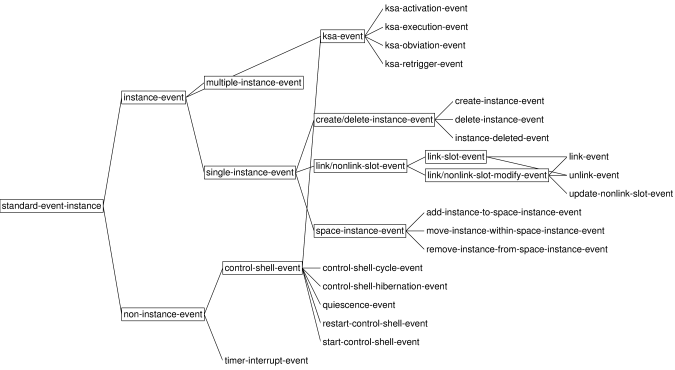
\includegraphics[scale=0.85]{agenda-shell-events}
\end{center}
\W\end{iftex}

\noindent Event classes shown within rectangles are abstract event classes
that cannot be signaled.  Nevertheless, abstract event classes are
very convenient if we wish to attach an event function to an entire
subtree of event classes.  We used abstract event classes to advantage
earlier when we enabled display of all control-shell events by
evaluating:
%
\begin{example}\color{darkergray}%
  gbbopen-user> (enable-event-printing '(control-shell-event :plus-subevents))
  nil
  gbbopen-user>
\end{example}


Add the following form at the end of your \code{tutorial-example.lisp} file:
%
\begin{example}
(add-event-function 'initializations 'start-control-shell-event
                    ;; Initializations should be done first!
                    :priority 100)
\end{example}

(We'll place the \textbf{add-event-function} form immediately after the
\code{initializations} function definition in our file, but this choice of
location is purely a code organizational style preference---the form could be
placed anywhere relative to the function definition.)

\subsection*{Step 3: Run the application}

\bfindex{start-control-shell}%
Start a fresh Common Lisp session, compile and load the
\code{tutorial-example.lisp} file directly from the editor buffer (using
\code{C-c C-k} in SLIME; \code{C-c C-b} in ELI) and start the Agenda Shell
again:
%
\begin{example}\color{darkergray}%
  gbbopen-user> \textcolor{black}{(start-control-shell)}
  ;; Control shell 1 started
  ;; No executable KSAs remain, exiting control shell
  ;; Control shell 1 exited: 3 cycles completed
  ;; Run time: 0 seconds
  ;; Elapsed time: 0 seconds
  :quiescence
  gbbopen-user>
\end{example}

Note that our developing application performs the same as it did in the last
exercise, but now our \code{initializations} event function is taking care of
all the details of starting up our application.  We no longer have to remember
to create the \code{known-world} space instance or to delete the blackboard
repository before running the application another time.

\subsection*{Step 4: Run it Again}

\bfindex{start-control-shell}%
Let's verify that we can re-run our application. Without doing anything else,
start the Agenda Shell again:
%
\begin{example}\color{darkergray}%
  gbbopen-user> \textcolor{black}{(start-control-shell)}
  ;; Control shell 1 started
  ;; No executable KSAs remain, exiting control shell
  ;; Control shell 1 exited: 3 cycles completed
  ;; Run time: 0 seconds
  ;; Elapsed time: 0 seconds
  :quiescence
  gbbopen-user>
\end{example}

As before our \code{initializations} event function took care of all the
details of starting up our application.

\subsection*{Step 5: It's a new world$\ldots$}

\bfindexit{make-space-instance}%
GBBopen allows us to restrict the classes of unit instances that can be stored
on a space instance.  For example, we can limit the \code{known-world} to
\code{location} unit instances by specifying an \code{:allowed-unit-classes}
value to \code{make-space-instance}:
%
\begin{example}\color{darkergray}%
  (defun initializations (event-name &key &allow-other-keys)
    (declare (ignore event-name))
    ;; Clean up any previous run:
    (delete-blackboard-repository)
    ;; Make a new known-world space instance:
    (make-space-instance 
     '(known-world)
     :dimensions '((x :ordered) (y :ordered))
     \textcolor{black}{:allowed-unit-classes 'location}))
\end{example}
%
Attempting to add any unit-instance that is not a \code{location} to
\code{known-world} will now generate an error.

It is often convenient to specify the dimensions of a space-instance relative
to those of one or more unit classes.  Edit the definition of
\code{initializations}, removing the \code{x} and \code{y} dimensions
specification:
%
\begin{example}\color{darkergray}%
(defun initializations (event-name &key &allow-other-keys)
  (declare (ignore event-name))
  ;; Clean up any previous run:
  (delete-blackboard-repository)
  ;; Make a new known-world space instance:
  (make-space-instance 
   '(known-world)
   :dimensions \textcolor{red}{'((x :ordered) (y :ordered))}
   :allowed-unit-classes 'location))
\end{example}
%
and replacing it with a call of \textbf{dimensions-of} to
obtain the dimensions associated with instances of the \code{location}
unit class:
%
\begin{example}\color{darkergray}%
(defun initializations (event-name &key &allow-other-keys)
  (declare (ignore event-name))
  ;; Clean up any previous run:
  (delete-blackboard-repository)
  ;; Make a new known-world space instance:
  (make-space-instance 
   '(known-world)
   :dimensions \textcolor{black}{(dimensions-of 'location)}
   :allowed-unit-classes 'location))
\end{example}

\subsection*{Step 6: Run the application again}

Compile and load the \code{tutorial-example.lisp} file directly from the
editor buffer (using \code{C-c C-k} in SLIME; \code{C-c C-b} in ELI) and start
the Agenda Shell again:
%
\begin{example}\color{darkergray}%
  gbbopen-user> \textcolor{black}{(start-control-shell)}
  ;; Control shell 1 started
  ;; No executable KSAs remain, exiting control shell
  ;; Control shell 1 exited: 3 cycles completed
  ;; Run time: 0 seconds
  ;; Elapsed time: 0 seconds
  :quiescence
  gbbopen-user>
\end{example}

\bfindexit{describe-space-instance}%
Verify the dimensionality of the \code{known-world} space instance by evaluating:
%
\begin{example}\color{darkergray}%
  gbbopen-user> \textcolor{black}{(describe-space-instance '(known-world))}
  Standard-space-instance #<standard-space-instance (known-world)>
    Allowed unit classes: t
    Dimensions:
      (x :ordered)
      (y :ordered)
  gbbopen-user>
\end{example}

%% ========================================================================
%%  Define Another KS

\T\markright{}%
\T\pagestyle{plain}
\T\cleardoublepage
\W\xname{tutorial-another-ks}
\T\pagestyle{fancy}
\T\thispagestyle{fancybottom}
\T\renewcommand{\headrulewidth}{0pt}
\section{Add Another KS}
\label{sec:another-ks}%

The last exercise made it easy to initialize and run our application
repeatedly by simply starting the Agenda Shell.  We also specified the
dimensionality of our \code{known-world} space instance relative to the
dimensional specifications of the \code{location} unit class.  With these
niceties in place, its time to move beyond our initial \code{location} unit
instance.

\fndocrule

This exercise shows you how to:
\begin{tightitemize}
\item Add an additional dimension to a unit class
\item Define a KS that obtains its execution-context information from its
  triggering unit instance
\item Extend the random-walk application to do some walking
\item Explore the resulting random walk
\end{tightitemize}

\fndocrule

\subsection*{Prerequisites}

\begin{tightitemize}
\item The \code{tutorial-example.lisp} file as modified thus far:
\end{tightitemize}

\begin{example}
(in-package :gbbopen-user)

(define-unit-class location ()
  (x y)
  (:dimensional-values
    (x :point x)
    (y :point y))
  (:initial-space-instances (known-world)))

(defmethod print-instance-slots ((location location) stream)
  (call-next-method)
  (when (and (slot-boundp location 'x)
             (slot-boundp location 'y))
    (format stream " (~s ~s)"
            (x-of location)
            (y-of location))))

;;; ======================================================================
;;;   Startup KS

(defun startup-ks-function (ksa)
  (declare (ignore ksa))
  ;; Create an initial location unit instance at (0,0):
  (make-instance 'location :x 0 :y 0))

(define-ks startup-ks
    :trigger-events ((start-control-shell-event))
    :execution-function 'startup-ks-function)

;;; ======================================================================
;;;   Initializations (run at Agenda Shell startup)

(defun initializations (event-name &key &allow-other-keys)
  (declare (ignore event-name))
  ;; Clean up any previous run:
  (delete-blackboard-repository)
  ;; Make a new known-world space instance:
  (make-space-instance 
   '(known-world)
   :dimensions (dimensions-of 'location)))

(add-event-function 'initializations 'start-control-shell-event
                    ;; Initializations should be done first!
                    :priority 100)
\end{example}

\begin{tightitemize}
\item The \code{:agenda-shell-user} module is loaded
\end{tightitemize}

\subsection*{Step 1: Add  another dimension}

It's time we introduce the notion of time to our application.  Edit the
\code{location} unit-class definition in \code{tutorial-example.lisp}, adding
a new slot, \code{time}, to the \code{location} unit class definition and a
corresponding \code{time} dimensional value:
%
\begin{example}\color{darkergray}%
(define-unit-class location ()
  (\textcolor{black}{time} 
   x y)
  (:dimensional-values
    \textcolor{black}{(time :point time)}
    (x :point x)
    (y :point y))
  (:initial-space-instances (known-world)))
\end{example}

Recall that we specified that the dimensions of the \code{known-world} space
instance that is created by our \code{initializations} function relative to
the dimensions of the \code{location} unit class:
%
\begin{example}\color{darkergray}%
  (make-space-instance 
      '(known-world)
      :dimensions (dimensions-of 'location)))
\end{example}
%
Therefore, we don't need to modify our call to \code{make-space-instance} in
order to add \code{time} as a dimension of \code{known-world}.

Next, modify \code{startup-ks-function} in \code{tutorial-example.lisp} so
that it creates the initial \code{location} unit instance at time 0:
%
\begin{example}\color{darkergray}%
(defun startup-ks-function (ksa)
  (declare (ignore ksa))
  ;; Create an initial location unit instance at (0,0) \textcolor{black}{at time 0}:
  (make-instance 'location \textcolor{black}{:time 0} :x 0 :y 0))
\end{example}

\subsection*{Step 2: A test of time}

Let's check our work.  Compile and load the
\code{tutorial-example.lisp} file directly from the editor buffer (using
\code{C-c C-k} in SLIME; \code{C-c C-b} in ELI) and start the Agenda Shell
again:
%
\begin{example}\color{darkergray}%
  gbbopen-user> \textcolor{black}{(start-control-shell)}
  ;; Control shell 1 started
  ;; No executable KSAs remain, exiting control shell
  ;; Control shell 1 exited: 3 cycles completed
  ;; Run time: 0 seconds
  ;; Elapsed time: 0 seconds
  :quiescence
  gbbopen-user>
\end{example}

\bfindexit{describe-instance}%
\bfindexit{find-instance-by-name}%
Check that the initial \code{location} unit instance is at \code{time} zero:
%
\begin{example}\color{darkergray}%
  gbbopen-user> \textcolor{black}{(describe-instance (find-instance-by-name 1 'location))}
  Location #<location 1 (0 0)>
    Instance name: 1
    Space instances: ((known-world))
    Dimensional values:
      time:  0
      x:  40
      y:  60
    Non-link slots:
      time:  0
      x:  40
      y : 60
    Link slots: None
  gbbopen-user>
\end{example}

\subsection*{Step 3: Define another KS}

Define a KS called \code{random-walk-ks} that:

\begin{tightitemize}
\item Is triggered when a \code{location} unit instance is created
\item Has a constant KSA rating of 100
\item Has an execution function called \code{random-walk-ks-function}, which:
\begin{tightitemize}
\item Checks if we've already walked for 75 locations and prints a message if
  we have. 
\item Otherwise:
\begin{tightitemize}
\item Determines a random location for which the x and y values are within 10
  of the x and y values of the triggering unit instance (that is, the
  \code{location} instance whose creation triggered the \code{random-walk-ks}
  KS)
\item If both of the x and y values for the new random location are between
  -50 and 50, creates a \code{location} unit instance at the random location;
  otherwise, prints a message indicating that we've walked off the world
\end{tightitemize}
\end{tightitemize}
\end{tightitemize}

\subsubsection*{Step 3a: Define a utility function}

Begin implementing the \code{random-walk-ks} by adding the following
utility function to the end of your \code{tutorial-example.lisp} file:

\begin{example}
;;; ======================================================================
;;;   Random-walk KS

(defun add-linear-variance (value max-variance)
  ;;; Returns a new random value in the interval
  ;;; [(- value max-variance), (+ value max-variance)]
  (+ value (- (random (1+ (* max-variance 2))) max-variance)))
\end{example}

Then compile the definition (using \code{C-c C-c} in SLIME or \code{C-c
  C-x} in ELI) and evaluate the following test in the REPL:

\bfindex{printv}%
\begin{example}\color{darkergray}%
  gbbopen-user> \textcolor{black}{(dotimes (i 15) (printv (add-linear-variance 0 10)))}
  ;;  (add-linear-variance 0 10) => 8
  ;;  (add-linear-variance 0 10) => 9
  ;;  (add-linear-variance 0 10) => 4
  ;;  (add-linear-variance 0 10) => 3
  ;;  (add-linear-variance 0 10) => -4
  ;;  (add-linear-variance 0 10) => -10
  ;;  (add-linear-variance 0 10) => -1
  ;;  (add-linear-variance 0 10) => 0
  ;;  (add-linear-variance 0 10) => 4
  ;;  (add-linear-variance 0 10) => 5
  ;;  (add-linear-variance 0 10) => 8
  ;;  (add-linear-variance 0 10) => -5
  ;;  (add-linear-variance 0 10) => -3
  ;;  (add-linear-variance 0 10) => 7
  ;;  (add-linear-variance 0 10) => 6
  nil
  gbbopen-user>
\end{example}

Because \code{add-linear-variance} is stochastic, your results will be
similar but not identical.  Note that we used GBBopen's \textbf{printv}
macro to display the result of each generated value.  \textbf{Printv} can
greatly assist debugging by printing forms and the results of evaluating
them.  \textbf{Printv} can be transparently wrapped around any form in a
complex function definition, as it evaluates and displays all the forms in
its body and returns the values resulting from evaluating the last form:

\begin{example}\color{darkergray}%
  gbbopen-user>  (printv "Some multiple values" (values 1 2) "Some more" (values 3 4 5))
  ;; Some multiple values
  ;;  (values 1 2) => 1; 2
  ;; Some more
  ;;  (values 3 4 5) => 3; 4; 5
  4
  5
  6
  gbbopen-user>
\end{example}

\subsubsection*{Step 3b: Define the \code{random-walk-ks} execution function}

Next add the following KS-execution function to the end of your
\code{tutorial-example.lisp} file:

\begin{example}
(defun random-walk-ks-function (ksa)
  ;;; Move to the next (random) location in the world
  (let* ((trigger-instance (sole-trigger-instance-of ksa))
         ;; The new time is one greater than the stimulus instance's time:
         (time (1+ (time-of trigger-instance))))
    (cond
     ;; If the maximum time value (75) is reached, tell the user we've
     ;; walked too long:
     ((>= time 75) (format t "~2&Walked too long.~\%"))
     (t ;; The new location is +/- 10 of the stimulus instance's location:
      (let ((x (add-linear-variance (x-of trigger-instance) 10))
            (y (add-linear-variance (y-of trigger-instance) 10)))
        (cond
         ;; Check that the new location is within the known-world
         ;; boundaries.  If so, create the new location instance:
         ((and (<= -50 x 50) (<= -50 y 50))
          (make-instance 'location 
            :time time 
            :x x 
            :y y))
         ;; Otherwise, tell the user that we've walked too far away:
         (t (format t "~2\&Walked off the world: (~d, ~d).~\%" x y))))))))
\end{example}

\bfindex{sole-trigger-instance-of}%
Unlike the KS-execution functions that we have defined previously,
\code{random-walk-ks-function} does not ignore its \code{ksa} argument.
Instead, it calls \textbf{sole-trigger-instance-of} with the \code{ksa}
unit-instance argument in order to obtain the \code{location} unit instance
whose creation triggered the KSA.  This pattern of obtaining the unit instance
that triggered a KSA and then using that triggering unit instance as the
context for the KS execution is typical of many KSs. 

\subsubsection*{Step 3c: Add the \code{random-walk-ks} definition}

Finally, add this \code{define-ks} form to the end of your
\code{tutorial-example.lisp} file to complete the \code{random-walk-ks}
definition:

\bfindexit{define-ks}%
\codeindex{quiescence-event}%
\begin{example}
(define-ks random-walk-ks
   :trigger-events ((create-instance-event location))
   :rating 100
   :execution-function 'random-walk-ks-function)
\end{example}

\subsection*{Step 4:  Run the application}

\bfindexit{start-control-shell}%
Compile and load the \code{random-walk-ks} forms, and then start the Agenda Shell:
%
\begin{example}\color{darkergray}%
  gbbopen-user> \textcolor{black}{(start-control-shell)}
  ;; Control shell 1 started

  Walked off the world: (23, 55).
  ;; No executable KSAs remain, exiting control shell
  ;; Control shell 1 exited: 64 cycles completed
  ;; Run time: 0.01 seconds
  ;; Elapsed time: 0 seconds
  :quiescence
  gbbopen-user>
\end{example}

\bfindexit{:dsbb}%
It looks like something happened! (Again, because \code{add-linear-variance}
is stochastic, your results will be similar but not identical.)  Let's look at
the blackboard repository and see how many \code{location} unit instances were
created:
%
\begin{example}\color{darkergray}%
  gbbopen-user> \textcolor{black}{:dsbb}

  Space Instance                Contents
  --------------                --------
  known-world                   61 instances (61 location)

  Unit Class                    Instances
  ----------                    ---------
  control-shell                         1 *
  ks                                    1 +
  ksa-queue                             2 +
  location                             61
  ordered-ksa-queue                     1 +
  standard-space-instance               1
                                ---------
                                       67 instances
  gbbopen-user>
\end{example}

The 61 \code{location} instances makes sense.  Previously, it required 3
control-shell cycles to create the initial \code{location} unit instance (one
to execute the \code{initial-ks} KSA followed by two additional cycles of
quiescence before the Agenda Shell exits).  We now create one additional
\code{location} unit instance with every execution of \code{random-walk-ks},
so we always create 3 fewer \code{location} instances than the total
number of control-shell cycles.

\subsection*{Step 5:  Where have we been?}

\bfindexit{map-instances-of-class}%
It would be interesting to see where our random walk has taken us.  We could
use GBBopen's \textbf{map-instances-of-class} iterator to print each of the
\code{location} unit instances:
%
\begin{example}\color{darkergray}%
  gbbopen-user> \textcolor{black}{(map-instances-of-class #'print 'location)}

  #<location 58 (5 31)> 
  #<location 13 (-7 10)> 
  #<location 26 (-40 35)> 
  #<location 39 (-4 3)> 
  #<location 52 (2 23)> 
  #<location 7 (3 17)> 
  #<location 20 (2 27)> 
  #<location 33 (-25 6)> 
  #<location 46 (-2 32)> 
       ...
  #<location 31 (-22 18)> 
  #<location 44 (-7 14)> 
  #<location 57 (2 41)> 
  #<location 12 (-15 15)> 
  #<location 25 (-32 38)> 
  #<location 38 (-10 -4)> 
  #<location 51 (-2 16)> 
  #<location 6 (10 27)> 
  #<location 19 (-1 17)> 
  #<location 32 (-25 12)> 
  #<location 45 (-7 23)> 
  nil
  gbbopen-user>
\end{example}
%
Unfortunately, the order that unit instances are supplied to the \code{print}
function is not controllable.  Our walk would be much clearer if we printed
the \code{location}s in time order.

\bfindexit{map-sorted-instances-of-class}%
We might consider taking advantage of the instance names that GBBopen assigns
to unit instances.  We could do something like the following:
%
\begin{example}\color{darkergray}%
  gbbopen-user> \textcolor{red}{(dotimes (i 76)
                  (let ((location (find-instance-by-name i 'location)))
                    (when location
                       (print location))))}

  #<location 1 (0 0)> 
  #<location 2 (10 4)> 
  #<location 3 (19 10)> 
  #<location 4 (14 9)> 
  #<location 5 (14 18)> 
  #<location 6 (10 27)> 
  #<location 7 (3 17)> 
  #<location 8 (-6 20)> 
  #<location 9 (4 15)> 
  #<location 10 (-5 14)> 
       ...
  #<location 50 (5 26)> 
  #<location 51 (-2 16)> 
  #<location 52 (2 23)> 
  #<location 53 (9 33)> 
  #<location 54 (7 43)> 
  #<location 55 (-2 36)> 
  #<location 56 (0 46)> 
  #<location 57 (2 41)> 
  #<location 58 (5 31)> 
  #<location 59 (13 39)> 
  #<location 60 (17 41)> 
  #<location 61 (21 50)> 
  nil
  gbbopen-user>
\end{example}

This is a bad idea for several reasons.  First, we are looking up every
\code{location} unit instance by its instance name, which is less efficient
than operating on \code{location} instances directly.  While this isn't an
significant issue in expressions that we evaluate in the REPL to investigate
our application, we should seek to avoid such inefficiencies in application
code.  More importantly, however, the \code{location} instance name just
happens to mirror the sequencing that we really want to display---the
\code{time} value of the \code{location}s.  We should find a way to sequence
\code{location} printing that relies on the \code{time} values directly.

\bfindex{map-sorted-instances-of-class}%
GBBopen provides a variant of \textbf{map-instances-of-class}, called
\textbf{map-sorted-instances-of-class}, that sorts the unit instances based on
a comparison predicate and an optional \code{:key} accessor function that
suits our needs:
%
\begin{example}\color{darkergray}%
  gbbopen-user> \textcolor{black}{(map-sorted-instances-of-class #'print 'location #'< 
                   :key #'time-of)}

  #<location 1 (0 0)> 
  #<location 2 (10 4)> 
  #<location 3 (19 10)> 
  #<location 4 (14 9)> 
  #<location 5 (14 18)> 
  #<location 6 (10 27)> 
  #<location 7 (3 17)> 
  #<location 8 (-6 20)> 
  #<location 9 (4 15)> 
  #<location 10 (-5 14)> 
       ...
  #<location 50 (5 26)> 
  #<location 51 (-2 16)> 
  #<location 52 (2 23)> 
  #<location 53 (9 33)> 
  #<location 54 (7 43)> 
  #<location 55 (-2 36)> 
  #<location 56 (0 46)> 
  #<location 57 (2 41)> 
  #<location 58 (5 31)> 
  #<location 59 (13 39)> 
  #<location 60 (17 41)> 
  #<location 61 (21 50)> 
  nil
  gbbopen-user>
\end{example}

\bfindex{do-sorted-instances-of-class}%
Using \textbf{map-sorted-instances-of-class} involves a sorting operation, so
this approach still has some efficiency concerns for use in application code.
However, it suits our REPL-exploration needs just fine.  (There is a
\textbf{do-sorted-instances-of-class} macro, if an iterative style is
preferred over a mapper.)  We will explore a more efficient approach to
displaying the random walk in the next exercise.

\subsection*{Step 6:  Run the application a few more times}

\bfindexit{start-control-shell}%
If we run the application a few more times, we eventually encounter a case
where we create the allotted 75 \code{location} unit instances without walking
off the \code{known-world}:
%
\begin{example}\color{darkergray}%
  gbbopen-user> \textcolor{black}{(start-control-shell)}
  ;; Control shell 1 started

  Walked too long.
  ;; No executable KSAs remain, exiting control shell
  ;; Control shell 1 exited: 78 cycles completed
  ;; Run time: 0.04 seconds
  ;; Elapsed time: 0 seconds
  :quiescence
  gbbopen-user>
\end{example}

\bfindexit{map-sorted-instances-of-class}%
Here is one such random walk:
%
\begin{example}\color{darkergray}%
  gbbopen-user> \textcolor{black}{(map-sorted-instances-of-class #'print 'location #'< 
                   :key #'time-of)}

  #<location 1 (0 0)> 
  #<location 2 (2 7)> 
  #<location 3 (-1 5)> 
  #<location 4 (-1 0)> 
  #<location 5 (3 -2)> 
  #<location 6 (13 -7)> 
  #<location 7 (8 -5)> 
  #<location 8 (1 2)> 
  #<location 9 (8 0)> 
  #<location 10 (5 8)> 
       ...
  #<location 70 (-13 -11)> 
  #<location 71 (-13 -6)> 
  #<location 72 (-9 -6)> 
  #<location 73 (1 -4)> 
  #<location 74 (-8 -11)> 
  #<location 75 (-13 -15)> 
  nil
  gbbopen-user>
\end{example}

%% ========================================================================
%%  Making Connections

\T\markright{}%
\T\pagestyle{plain}
\T\cleardoublepage
\W\xname{tutorial-connections}
\T\pagestyle{fancy}
\T\thispagestyle{fancybottom}
\T\renewcommand{\headrulewidth}{0pt}
\section{Making Connections}
\label{sec:connections}%

%\begin{center}
%\textcolor{caution}{[Construction ahead...]}
%\end{center}

We finally did some walking in the last exercise and learned how to display
the \code{location}s in our walk from the REPL.  In this exercise, we learn
how to use GBBopen's link capabilities to represent relationships among unit
instances.  Links are an important aspect of almost every GBBopen application,
so it's time that we started taking advantage of them.

\fndocrule

This exercise shows you how to:
\begin{tightitemize}
\item Add link slots to a unit class
\item Use link slots to traverse and display the resulting random walk
\end{tightitemize}

\fndocrule

\subsection*{Prerequisites}

\begin{tightitemize}
\item The \code{tutorial-example.lisp} file as modified thus far:
\end{tightitemize}

\begin{example}
(in-package :gbbopen-user)

(define-unit-class location ()
  (time 
   x y)
  (:dimensional-values
    (time :point time)
    (x :point x)
    (y :point y))
  (:initial-space-instances (known-world)))

(defmethod print-instance-slots ((location location) stream)
  (call-next-method)
  (when (and (slot-boundp location 'x)
             (slot-boundp location 'y))
    (format stream " (~s ~s)"
            (x-of location)
            (y-of location))))

;;; ======================================================================
;;;   Startup KS

(defun startup-ks-function (ksa)
  (declare (ignore ksa))
  ;; Create an initial location unit instance at (0,0):
  (make-instance 'location :time 0 :x 0 :y 0))

(define-ks startup-ks
    :trigger-events ((start-control-shell-event))
    :execution-function 'startup-ks-function)

;;; ======================================================================
;;;   Initializations (run at Agenda Shell startup)

(defun initializations (event-name &key &allow-other-keys)
  (declare (ignore event-name))
  ;; Clean up any previous run:
  (delete-blackboard-repository)
  ;; Make a new known-world space instance:
  (make-space-instance 
   '(known-world)
   :dimensions (dimensions-of 'location)))

(add-event-function 'initializations 'start-control-shell-event
                    ;; Initializations should be done first!
                    :priority 100)

;;; ======================================================================
;;;   Random-walk KS

(defun add-linear-variance (value max-variance)
  ;;; Returns a new random value in the interval
  ;;; [(- value max-variance), (+ value max-variance)]
  (+ value (- (random (1+ (* max-variance 2))) max-variance)))

(defun random-walk-ks-function (ksa)
  ;;; Move to the next (random) location in the world
  (let* ((trigger-instance (sole-trigger-instance-of ksa))
         ;; The new time is one greater than the stimulus instance's time:
         (time (1+ (time-of trigger-instance))))
    (cond
     ;; If the maximum time value (75) is reached, tell the user we've
     ;; walked too long:
     ((>= time 75) (format t "~2&Walked too long.~\%"))
     (t ;; The new location is +/- 10 of the stimulus instance's location:
      (let ((x (add-linear-variance (x-of trigger-instance) 10))
            (y (add-linear-variance (y-of trigger-instance) 10)))
        (cond
         ;; Check that the new location is within the known-world
         ;; boundaries.  If so, create the new location instance:
         ((and (<= -50 x 50) (<= -50 y 50))
          (make-instance 'location 
            :time time 
            :x x 
            :y y))
         ;; Otherwise, tell the user that we've walked too far away:
         (t (format t "~2&Walked off the world: (~d, ~d).~\%" x y))))))))

(define-ks random-walk-ks
    :trigger-events ((create-instance-event location))
    :rating 100
    :execution-function 'random-walk-ks-function)
\end{example}

\begin{tightitemize}
\item The \code{:agenda-shell-user} module is loaded
\end{tightitemize}

\subsection*{Step 1: Add  a link}

In the last exercise, we used \textbf{map-sorted-instances-of-class} to
display the random walk.  Another way that we could represent the walk is by
connect each newly created \code{location} unit instance to the
\code{location} unit instance that preceded it in the walk.  We'll use
GBBopen's link capabilities to do this.

A \textit{link} is a bidirectional relationship between two unit instances
that is implemented by two pointers. From the perspective of a particular unit
instance, each link consists of an outgoing, or \textit{direct}, pointer to
another unit instance and an incoming, or \textit{inverse}, pointer that is
stored in unit instance pointed to by the direct pointer.  GBBopen
automatically maintains the bidirectional-link consistency of these pointers
when creating new links, deleting existing links, or deleting unit instances.
Links remove the possibility of ``one-sided'' relationships or ``dangling''
pointers to deleted unit instances.

Edit the \code{location} unit-class definition in your
\code{tutorial-example.lisp} file, adding two link slots, \code{next-location}
and \code{previous-location}, to the \code{location} unit class definition:
%
\begin{example}\color{darkergray}%
(define-unit-class location ()
  (time 
   x y
   \textcolor{black}{(next-location
    :link (location previous-location :singular t) 
    :singular t)
   (previous-location
    :link (location next-location :singular t)  
    :singular t)})
  (:dimensional-values
    (time :point time)
    (x :point x)
    (y :point y))
  (:initial-space-instances (known-world)))
\end{example}

Each link-slot specification is a list whose first element is the name of the
link slot.  This is followed by the link slot option \code{:link} and a
concise specification of the inverse link slot associated with that link slot.
In this case, the \code{next-location}/\code{previous-location} link is
between instances of the same (\code{location}) unit class, but often links
are between instances of different unit classes. 

Links can be many-to-many, many-to-one, one-to-many, or one-to-one.  In this
case, the \code{next-location}/\code{previous-location} link is one-to-one,
which is specified by including the \code{:singular t} slot option in the
link-slot definition (and the corresponding \code{:singular t} specification
in the concise inverse-link-slot specification).  To help clarify the
specification of link slot arity, let's temporarily assume that we want a
\code{location} instance that can have many next locations, but only a single
previous location.  This link relation would be specified as follows:
%
\begin{example}\color{darkergray}%
    ...
 \textcolor{blue}{(next-locations
  :link (location previous-location :singular t)))
 (previous-location
  :link (location next-locations)  
  :singular t)}
    ...
\end{example}

We've followed the natural GBBopen convention of giving singular link
slots a singular name (such as \code{previous-location}) and link
slots that can contain multiple links a plural name (such as
\code{next-locations}).  Note that the \code{:singular} option is
associated with the \code{previous-location} link slot as both a slot
option in the \code{previous-location} link-slot definition and in the
concise inverse-link-slot specification for \code{previous-location}
in the \code{next-locations} link-slot definition.

\subsection*{Step 2: Break some links}

The concise inverse-link-slot specification supplied by the
\code{:link} slot option provides a ``double entry'' redundancy that
is useful when links are between instances of different unit classes,
as the link can be understood by viewing either class definition.  The
redundancy also helps GBBopen recognize inconsistencies in link
specifications.  The function \textbf{check-link-consistency} asks
GBBopen to validate that all link definitions are consistent.  Let's
try it on our current random-walk application.  Compile and load the
latest changes in your \code{tutorial-example.lisp} file (including
the new \code{next-location} and \code{previous-location} link slots).
Then check link consistency:
%
\begin{example}\color{darkergray}%
  gbbopen-user> \textcolor{black}{(check-link-consistency)}
  ;; All link definitions are consistent.
  t
  gbbopen-user>
\end{example}
%
GBBopen reports that all link definitions are consistent.

Suppose that we had forgotten to add the \code{previous-location} end
of the link in our \code{location} unit-class definition. Edit the
\code{location} unit-class definition in your
\code{tutorial-example.lisp} file, adding the line \code{\#+ignore}
immediately before the \code{previous-location} link-slot definition:
%
\begin{example}\color{darkergray}%
(define-unit-class location ()
  (time 
   x y
   (next-location
    :link (location previous-location :singular t) 
    :singular t)
    \textcolor{black}{\#+ignore}     
   (previous-location
    :link (location next-location :singular t)  
    :singular t))
  (:dimensional-values
    (time :point time)
    (x :point x)
    (y :point y))
  (:initial-space-instances (known-world)))
\end{example}

The \code{\#+ignore} read-time conditionalization tells Common Lisp to
skip over the next form if \code{ignore} is not an element of the
feature list \code{*features*}.  By convention, \code{ignore} is never
added to \code{*features*}, so \code{\#+ignore} is a handy mechanism
for temporarily ``commenting out'' a single form.

Compile the now-defective definition (using \code{C-c C-c} in SLIME or
\code{C-c C-x} in ELI) and then recheck link consistency:
%
\begin{example}\color{darkergray}%
  gbbopen-user> \textcolor{black}{(check-link-consistency)}
  Warning: The inverse of link slot next-location in unit class location 
           refers to link slot previous-location which is not present in 
           unit class location.
  nil
  gbbopen-user>
\end{example}
%
As expected, GBBopen alerts us to the problem.

Remove the \code{\#+ignore} that we just added and comment out the
\code{:singular t} portion of the inverse link-slot specification in 
\code{next-location}:
%
\begin{example}\color{darkergray}%
(define-unit-class location ()
  (time 
   x y
   (next-location
    :link (location previous-location\textcolor{black}{) ;} :singular t) 
    :singular t)
    \textcolor{red}{#+ignore}     
   (previous-location
    :link (location next-location :singular t)  
    :singular t))
  (:dimensional-values
    (time :point time)
    (x :point x)
    (y :point y))
  (:initial-space-instances (known-world)))
\end{example}

Compile the again-defective definition (using \code{C-c C-c} in SLIME or
\code{C-c C-x} in ELI) and then recheck link consistency:
%
\begin{example}\color{darkergray}%
  gbbopen-user> \textcolor{black}{(check-link-consistency)}
  Warning: Link slot next-location in unit class location incorrectly 
           declares its inverse link slot previous-location in unit 
           class location as not singular.
  nil
  gbbopen-user>
\end{example}
%
Once again, GBBopen has alerted us to the problem.

Restore the \code{:singular t} portion of the inverse link-slot
specification in \code{next-location} that we just commented out:
%
\begin{example}\color{darkergray}%
(define-unit-class location ()
  (time 
   x y
   (next-location
    :link (location previous-location\textcolor{red}{) ;} :singular t) 
    :singular t)
   (previous-location
    :link (location next-location :singular t)  
    :singular t))
  (:dimensional-values
    (time :point time)
    (x :point x)
    (y :point y))
  (:initial-space-instances (known-world)))
\end{example}

Then recompile and recheck link consistency:
%
\begin{example}\color{darkergray}%
  gbbopen-user> \textcolor{black}{(check-link-consistency)}
  ;; All link definitions are consistent.
  t
  gbbopen-user>
\end{example}

\subsection*{Step 3: Create some links}

Let's use our newly defined \code{next-location}/\code{previous-location} link
to connect our \code{location} unit instances.  Edit the
\code{random-walk-ks-function} definition in your \code{tutorial-example.lisp}
file, adding the trigger instance as a new \code{:previous-location} argument
to \code{make-instance}:
%
\begin{example}\color{darkergray}%
(defun random-walk-ks-function (ksa)
  ;;; Move to the next (random) location in the world
  (let* ((trigger-instance (sole-trigger-instance-of ksa))
         ;; The new time is one greater than the stimulus instance's time:
         (time (1+ (time-of trigger-instance))))
    (cond
     ;; If the maximum time value (75) is reached, tell the user we've
     ;; walked too long:
     ((>= time 75) (format t "~2&Walked too long.~\%"))
     (t ;; The new location is +/- 10 of the stimulus instance's location:
      (let ((x (add-linear-variance (x-of trigger-instance) 10))
            (y (add-linear-variance (y-of trigger-instance) 10)))
        (cond
         ;; Check that the new location is within the known-world
         ;; boundaries.  If so, create the new location instance:
         ((and (<= -50 x 50) (<= -50 y 50))
          (make-instance 'location 
            :time time 
            :x x 
            :y y
            \textcolor{black}{:previous-location trigger-instance}))
         ;; Otherwise, tell the user that we've walked too far away:
         (t (format t "~2&Walked off the world: (~d, ~d).~\%" x y))))))))
\end{example}

Compile the \code{random-walk-ks-function} (using \code{C-c C-c} in SLIME or
\code{C-c C-x} in ELI) and then run the application:
%
\begin{example}\color{darkergray}%
  gbbopen-user> \textcolor{black}{(start-control-shell)}
  ;; Control shell 1 started

  Walked off the world: (55, 35).
  ;; No executable KSAs remain, exiting control shell
  ;; Control shell 1 exited: 66 cycles completed
  ;; Run time: 0.01 seconds
  ;; Elapsed time: 0 seconds
  :quiescence
  gbbopen-user>
\end{example}

Let's describe a couple of \code{location} unit instances to check our work.
First, the initial \code{location} unit instance:
%
\begin{example}\color{darkergray}%
  gbbopen-user> \textcolor{black}{(describe-instance (find-instance-by-name 1 'location))}
  Location #<location 1 (0 0)>
    Instance name: 1
    Space instances: ((known-world))
    Dimensional values:
      time:  0
      x:  40
      y:  60
    Non-link slots:
      time:  0
      x:  40
      y:  60
    Link slots:
      next-location:  #<location 2 (-10 10)>
      previous-location:  nil
  gbbopen-user>
\end{example}

Note that the \code{next-location} link slot points to the next
\code{location} unit instance in our random walk.  Let's describe that
unit instance:
%
\begin{example}\color{darkergray}%
  gbbopen-user> \textcolor{black}{(describe-instance (find-instance-by-name 2 'location))}
  Location #<location 2 (-10 10)>
    Instance name: 2
    Space instances: ((known-world))
    Dimensional values:
      time:  1
      x:  -10
      y:  10
    Non-link slots:
      time:  1
      x:  -10
      y:  10
    Link slots:
      next-location:  #<location 3 (-6 19)>
      previous-location:  #<location 1 (0 0)>
  gbbopen-user>
\end{example}

Its \code{next-location} link slot points to the third \code{location} unit
instance in our random walk and its \code{previous-location} link slot points
back to the initial \code{location} unit instance.

We can now follow the links to display the random walk:
%
\begin{example}\color{darkergray}%
  gbbopen-user> \textcolor{black}{(loop with location = (find-instance-by-name 1 'location) 
                  do (print location)
                  while (setf location (next-location-of location)))}

  #<location 1 (0 0)> 
  #<location 2 (-10 10)> 
  #<location 3 (-6 19)> 
  #<location 4 (0 14)> 
  #<location 5 (-1 14)> 
  #<location 6 (8 10)> 
  #<location 7 (17 3)> 
  #<location 8 (7 -6)> 
  #<location 9 (10 4)> 
  #<location 10 (5 -5)> 
       ...
  #<location 60 (29 17)> 
  #<location 61 (31 21)> 
  #<location 62 (40 23)> 
  #<location 63 (45 28)> 
  nil
  gbbopen-user>
\end{example}

\subsection*{Step 4: Define a ``print walk'' KS}

\bfindexit{define-ks}%
\codeindex{:stop}%
\codeindex{quiescence-event}%
\bfindexit{find-instance-by-name}%
Let's add a new KS, \code{print-walk-ks}, that displays the random walk once
it is completed. Add the following KS to the end of your
\code{tutorial-example.lisp} file:
%
\begin{example}
;;; ======================================================================
;;;   Print-walk KS

(defun print-walk-ks-function (ksa)
  ;;; Starting with the initial location instance, print the instance name
  ;;; and location of the walk
    (declare (ignore ksa))
    (format t "~2\&The random walk:~\%")
      (let ((instance (find-instance-by-name 1 'location)))
      (while instance
        (format t "~s (~s ~s)~\%"
                (instance-name-of instance)
                (x-of instance)
                (y-of instance))
        (setf instance (next-location-of instance))))
    ;; Tell the Agenda Shell to exit:
    ':stop)

  (define-ks print-walk-ks
    :trigger-events ((quiescence-event))
    :rating 100
    :execution-function 'print-walk-ks-function)
\end{example}
%
The \code{print-walk-ks} is triggered by a \code{quiescence-event}.  Recall
that the Agenda Shell signals that quiescence has occurred when no
executable KSAs are available to be executed and then it continues for an
additional KS-execution cycle in case any executable KSAs resulted from the
quiescence event.  So, \code{print-walk-ks} will be triggered once no
\code{random-walk-ks} KSAs are triggered by newly created \code{location} unit
instances.

The \code{print-walk-ks-function} follows the
\code{next-location}/\code{previous-location} link to display the walk.  More
importantly, the function returns the keyword symbol \code{:stop}.  The Agenda
Shell checks the value returned by a KS execution function for this special
indicator and, if it is returned, the control shell is exited.  If we did not
return \code{:stop}, the \code{print-walk-ks} KS would be triggered and
activated on the first \code{quiescence-event}, the KSA would execute, then
the Agenda Shell would detect another quiescence condition, signal a new
\code{quiescence-event}, and our application would print the random walk over
and over again.

Let's compile our latest changes and then run our application with the new
\code{print-walk-ks} KS in place:
%
\begin{example}\color{darkergray}%
  gbbopen-user> \textcolor{black}{(start-control-shell)}
  ;; Control shell 1 started

  Walked off the world: (54, 15).

  The random walk:
  1 (0 0)
  2 (-6 9)
  3 (-14 8)
  4 (-5 6)
  5 (-13 5)
  6 (-11 13)
  7 (-11 4)
  8 (-17 8)
  9 (-21 15)
  10 (-12 14)
       ...
  35 (40 28)
  36 (50 22)
  37 (49 12)
  38 (47 10)
  ;; Explicit :stop issued by KS print-walk-ks
  ;; Control shell 1 exited: 41 cycles completed
  ;; Run time: 0.01 seconds
  ;; Elapsed time: 0 seconds
  :stop
  gbbopen-user>
\end{example}

%% ========================================================================
%%  Creating an Application

\T\markright{}%
\T\pagestyle{plain}
\T\cleardoublepage
\W\xname{tutorial-application}
\T\pagestyle{fancy}
\T\thispagestyle{fancybottom}
\T\renewcommand{\headrulewidth}{0pt}
\section{Creating a GBBopen Application}
\label{sec:application}%

GBBopen's \xreflink{Mini Module system}{sec:mini-module} provides facilities
that make it easy to define and use your own GBBopen applications.

\fndocrule

This exercise shows you how to:
\begin{tightitemize}
\item Structure an application using the \xreflink{Mini Module
    system}{sec:mini-module}
\item Define a top-level REPL command for your application
\item Compile and load your application using your REPL command
\item Create and use an application-specific package
\item Add an ``autorun'' form 
\end{tightitemize}

\fndocrule

\subsection*{Prerequisites}

\begin{tightitemize}
\item The \code{tutorial-example.lisp} file as modified thus far:

\begin{example}
(in-package :gbbopen-user)

(define-unit-class location ()
  (time 
   x y
   (next-location
    :link (location previous-location :singular t) 
    :singular t)
   (previous-location
    :link (location next-location :singular t)  
    :singular t))
  (:dimensional-values
    (time :point time)
    (x :point x)
    (y :point y))
  (:initial-space-instances (known-world)))

(defmethod print-instance-slots ((location location) stream)
  (call-next-method)
  (when (and (slot-boundp location 'x)
             (slot-boundp location 'y))
    (format stream " (~s ~s)"
            (x-of location)
            (y-of location))))

;;; ======================================================================
;;;   Startup KS

(defun startup-ks-function (ksa)
  (declare (ignore ksa))
  ;; Create an initial location unit instance at (0,0):
  (make-instance 'location :time 0 :x 0 :y 0))

(define-ks startup-ks
    :trigger-events ((start-control-shell-event))
    :execution-function 'startup-ks-function)

;;; ======================================================================
;;;   Initializations (run at Agenda Shell startup)

(defun initializations (event-name &key &allow-other-keys)
  (declare (ignore event-name))
  ;; Clean up any previous run:
  (delete-blackboard-repository)
  ;; Make a new known-world space instance:
  (make-space-instance 
   '(known-world)
   :dimensions (dimensions-of 'location)))

(add-event-function 'initializations 'start-control-shell-event
                    ;; Initializations should be done first!
                    :priority 100)

;;; ======================================================================
;;;   Random-walk KS

(defun add-linear-variance (value max-variance)
  ;;; Returns a new random value in the interval
  ;;; [(- value max-variance), (+ value max-variance)]
  (+ value (- (random (1+ (* max-variance 2))) max-variance)))

(defun random-walk-ks-function (ksa)
  ;;; Move to the next (random) location in the world
  (let* ((trigger-instance (sole-trigger-instance-of ksa))
         ;; The new time is one greater than the stimulus instance's time:
         (time (1+ (time-of trigger-instance))))
    (cond
     ;; If the maximum time value (75) is reached, tell the user we've
     ;; walked too long:
     ((>= time 75) (format t "~2&Walked too long.~\%"))
     (t ;; The new location is +/- 10 of the stimulus instance's location:
      (let ((x (add-linear-variance (x-of trigger-instance) 10))
            (y (add-linear-variance (y-of trigger-instance) 10)))
        (cond
         ;; Check that the new location is within the known-world
         ;; boundaries.  If so, create the new location instance:
         ((and (<= -50 x 50) (<= -50 y 50))
          (make-instance 'location 
            :time time 
            :x x 
            :y y
            :previous-location trigger-instance))
         ;; Otherwise, tell the user that we've walked too far away:
         (t (format t "~2\&Walked off the world: (~d, ~d).~\%" x y))))))))

(define-ks random-walk-ks
    :trigger-events ((create-instance-event location))
    :rating 100
    :execution-function 'random-walk-ks-function)

;;; ======================================================================
;;;   Print-walk KS

(defun print-walk-ks-function (ksa)
  ;;; Starting with the initial location instance, print the instance name
  ;;; and location of the walk
  (declare (ignore ksa))
  (format t "~2\&The random walk:~\%")
    (let ((instance (find-instance-by-name 1 'location)))
    (while instance
      (format t "~s (~s ~s)~\%"
              (instance-name-of instance)
              (x-of instance)
              (y-of instance))
      (setf instance (next-location-of instance))))
  ;; Tell the Agenda Shell to exit:
  ':stop)

(define-ks print-walk-ks
  :trigger-events ((quiescence-event))
  :rating 100
  :execution-function 'print-walk-ks-function)
\end{example}

\item The GBBopen environment setup using
  \code{\var{<install-dir>\/}/gbbopen-init.lisp} as described in Steps 1 and 2
  of the \reflink{Enhancing Your Development Environment
    exercise}{sec:environment}
\end{tightitemize}

\subsection*{Step 1: Create your personal \code{gbbopen-modules} directory}

Create a directory named \code{gbbopen-modules} in your \reflink{``homedir''
  directory}{ref:your-homedir}.  For example:
%
\begin{example}\color{darkergray}%
  [~]\$ \textcolor{black}{mkdir gbbopen-modules}
  [~]\$ 
\end{example}
%
This is a special directory that is read by used by GBBopen to find
applications when GBBopen is started using
\code{\var{<install-dir>\/}/gbbopen-init.lisp}, as described in Steps 1 and 2
of the \reflink{Enhancing Your Development Environment
  exercise}{sec:environment}.

\subsection*{Step 2: Create a module-definition file for the random-walk application}

Recall that you created a directory to hold the random-walk application in Step 1
of \reflink{Working Within a File exercise}{sec:file}.  I used these shell
commands to create my directories:
%
\begin{example}\color{darkergray}%
  [~]\$ mkdir tutorial
  [~]\$ cd tutorial
  [~/tutorial]\$ mkdir source
  [~/tutorial]\$ 
\end{example}
%
Then you created the \code{tutorial-example.lisp} file in this \code{source}
subdirectory. We said that we would explain why we created the \code{source}
directory in a later exercise.  Well, later has arrived.

Each GBBopen application is packaged in a directory that contains:
\begin{tightitemize}
\item a \code{modules.lisp} file that contains module definitions (loaded
  after the personal \code{\var{<install-dir>\/}/gbbopen-init.lisp} file if
  there is one in the user's ``homedir'')
\item a directory named \code{source} containing all the source files for the
  module or application
\item an optional \code{commands.lisp} file that specifies top-level commands
  for the module (loaded after the personal \code{gbbopen-commands.lisp} file
  if there is one in the user's ``homedir'')
\end{tightitemize}
%
You already have the \code{source} directory and the
\code{tutorial-example.lisp} source file.  Next, we create the
\code{modules.lisp} file for the application.  (We will create a
\code{commands.lisp} file for the random-walk application in Step 5.)

Use your Common Lisp editor to create a new file named \code{modules.lisp} in
the \code{tutorial} directory (just as you created the
\code{tutorial-example.lisp} file in Step 2 of \reflink{Working Within a File
  exercise}{sec:file}.  Note that this file is \textit{not\/} in the
\code{source} subdirectory, but in the \code{tutorial} directory that contains
the \code{source} subdirectory.

Type the following two forms into the new \code{modules.lisp}
file:
%
\begin{example}
(in-package :common-lisp-user)

(define-module :tutorial
  (:requires :agenda-shell-user)
  (:files "tutorial-example"))
\end{example}
%
and then save the file.

Recall that the \code{in-package} form specifies the Common Lisp package that
is made current when the file is compiled or loaded.  A \code{modules.lisp}
file should always specify the \code{:mini-module-user} package as the first
form in the file.

The second form defines our application module, which we will name
\code{:tutorial}.  The \code{:requires} subform specifies that the
\code{:agenda-shell-user} module must be compiled (if necessary) and then
loaded before our \code{:tutorial} module.  The \code{:files} subform
specified the files that comprise the module. In our case, there is one file:
\code{tutorial-example.lisp}.  We leave off the \code{.lisp} file extension,
as the \xreflink{Mini Module system}{sec:mini-module} will add the appropriate
source or compiled file extension for us.

\subsection*{Step 3: Add the random-walk application to your personal
  \code{gbbopen-modules} directory}

The \code{gbbopen-modules} directory in your ``homedir'' is expected to
consist of directories each containing an individual GBBopen application.  We
could place the random-walk application directly in the \code{gbbopen-modules}
directory by moving the \code{tutorial} directory there.  However, it is
generally more convenient to use a symbolic link to point to the actual
application directory.  For example, an application can be provided to a
number of users by creating a symbolic link to the application directory in
each user's \code{gbbopen-modules} directory.

Unless you are running Windows, add the random-walk application to your
\code{gbbopen-applications} by creating a symbolic link.  For example:
%
\begin{example}\color{darkergray}%
  [~]\$ \textcolor{black}{cd ~/gbbopen-modules/}
  [~]\$ \textcolor{black}{ln -s ~/tutorial .}
  [~]\$ 
\end{example}

\subsubsection*{Windows users}

Instead of creating a symbolic link, GBBopen also supports a special ``pseudo
symbolic-link'' file that can be used with Windows.  This is simply a text
file of type \code{.sym} that contains the target directory path as the sole
line in the file.  For example, you could create the file \code{tutorial.sym}
in your \code{gbbopen-modules} directory with:
%
\begin{example}
  C:\bkslash{}tutorial\bkslash
\end{example}
\T\vskip -12pt
%
as the sole line in the file.

\subsection*{Step 4: Try the \code{:tutorial} module definition}

Let's try out our module definition.  Exit Common Lisp and start a fresh
Common Lisp session.  If you have set up your environment according to the
\reflink{Enhancing Your Development Environment exercise}{sec:environment},
the following files should be loaded:
%
\begin{example}\color{darkergray}%
     ...
  ;; Loading \var{<homedir\/>}/shared-init.lisp
  ;;   Loading \var{<install-dir\/>}/gbbopen-init.lisp
  ;;     Loading \var{<install-dir\/>}/extended-repl.lisp
  ;;     Loading \var{<install-dir\/>}/commands.lisp
  ;;     Loading \var{<install-dir\/>}/gbbopen-modules-directory.lisp
  ;; Loading module command definitions from \var{<homedir\/>}/gbbopen-modules/...
  cl-user>
\end{example}

Note that some basic GBBopen initialization files have been loaded for us (but
no command definitions yet) and that GBBopen itself (or even the Mini Module
system) are not loaded by \code{\var{<install-dir>\/}/gbbopen-init.lisp}.

Now, instead of loading the \code{:agenda-shell-user} module, let's load only
the \code{:mini-module-user} module:

%
\begin{example}\color{darkergray}%
  cl-user> \textcolor{black}{:mini-module-user}
  ;; Loading \var{<install-dir\/>}/startup.lisp
     ...
  ;;   Loading \var{<install-dir\/>}/\var{<platform-dir\/>}/mini-module/mini-module-user.fasl
  ;;   Loading \var{<install-dir\/>}/modules.lisp
  ;; Loading module definitions from \var{<homedir\/>}/gbbopen-modules/...
  ;;     Loading \var{<homedir\/>}/tutorial/modules.lisp
  mini-module-user>
\end{example}

Note that when the Mini Module system was loaded as part of loading the
\code{:mini-module-user} module, the module definitions for our personal
GBBopen modules were loaded automatically.  (In this case, the
\code{\var{<homedir>\/}/tutorial/modules.lisp} file.)  Now that our
\code{:tutorial} module has been defined, we can use the
\textbf{compile-module} REPL command, \code{:cm}, to compile (if needed) and
load our application module:
%
\begin{example}\color{darkergray}%
  mini-module-user> \textcolor{black}{:cm :tutorial}
  ;;   Loading \var{<install-dir\/>}/\var{<platform-dir\/>}/tools/portable-threads.fasl
     ...
  ;;   Loading .../gbbopen/control-shells/agenda-shell-user.fasl

  Error: Directory \var{<homedir\/>}/tutorial/\var{<platform-dir\/>}/ 
         in module :tutorial doesn't exist.

  Restart actions (select using :c n):
    0: Create this directory.
    1: Create this directory and any future missing directories.
  mini-module-user>>
\end{example}
%
The \code{:requires} in our \code{:tutorial} module definition causes the
\code{:agenda-shell-user} module (and its required modules) to be loaded for
us.  Then the Mini Module system stops with a continuable error, telling us
that the directory to hold the compiled application files does not exist.  The
compiled files are put in a Common Lisp and platform-specific subdirectory,
\code{<\var{platform-dir>\/}}, in our \code{tutorial} directory that mirrors
the \code{source} directory.  This organization makes it easy to use the
application with a number of Common Lisp implementations and on a file system
shared with a number of different hosts and operating systems.

We could have avoided this continuable error by providing the
\code{:create-dirs} option to the \code{:cm} command:
\begin{example}\color{darkergray}%
  mini-module-user> :cm :tutorial :create-dirs
\end{example}
%
to allow the Mini Module system to create the \code{<\var{platform-dir>\/}}
subdirectory automatically for us.  Since we did not do this, we can still
continue from the error:
%
\begin{example}\color{darkergray}%
  Restart actions (select using :c n):
    0: Create this directory.
    1: Create this directory and any future missing directories.
  mini-module-user>> \textcolor{black}{:c 0}
  ;; Compiling file \var{<homedir\/>}/tutorial/source/tutorial-example.lisp
  ;; Loading \var{<homedir\/>}/tutorial/\var{<platform-dir\/>}/tutorial-example.fasl
  mini-module-user>
\end{example}

At this point, we've compiled and loaded our \code{:tutorial} application
module.

\subsection*{Step 5: Create a command-definition file for the random-walk
  application}

It is convenient to define a REPL command to compile and load you application
(and any required GBBopen modules).  

Use your Common Lisp editor to create a new file named \code{commands.lisp} in
the \code{tutorial} directory. Type the following two forms into the new
\code{commands.lisp} file:
%
\begin{example}
(in-package :common-lisp-user)

(define-tll-command :tutorial (\&rest options)
  "Compile and load the Random-Walk Tutorial Application Module"
  (startup-module :tutorial options :gbbopen-user))
\end{example}

%
and then save the file.

A \code{commands.lisp} file should always specify the \code{:common-lisp-user}
package as the first form in the file.

The \textbf{define-tll-command} form adds a top-level REPL command, named
\code{:tutorial}, to the set of handy REPL commands.  The
\textbf{startup-module} call does all the work associated with executing the
command.  The first argument to \textbf{startup-module} specifies that the
\code{:tutorial} module will be compiled (if necessary) and then loaded by the
\xreflink{Mini Module system}{sec:mini-module} when the \code:{tutorial}
command is issued.  The second, \code{options}, argument passes any options
given with the command to a \textbf{compile-module} call that is performed by
\textbf{startup-module}.  The third argument, \code{:gbbopen-user} is optional
and specifies that the REPL's current package should be changed to \code{:gbbopen-user} after the \code{:tutorial} module is loaded. 

\subsection*{Step 6: Try the \code{:tutorial} command}

Let's try our command definition.  Exit Common Lisp and start a fresh
Common Lisp session.  If you have set up your environment according to the
\reflink{Enhancing Your Development Environment exercise}{sec:environment},
the following files should be loaded:
%
\begin{example}\color{darkergray}%
     ...
  ;; Loading \var{<homedir\/>}/shared-init.lisp
  ;;   Loading \var{<install-dir\/>}/gbbopen-init.lisp
  ;;     Loading \var{<install-dir\/>}/extended-repl.lisp
  ;;     Loading \var{<install-dir\/>}/commands.lisp
  ;;     Loading \var{<install-dir\/>}/gbbopen-modules-directory.lisp
  ;; Loading module command definitions from \var{<homedir\/>}/gbbopen-modules/...
  ;      Loading \var{<homedir>}/gbbopen-modules/tutorial/commands.lisp
  cl-user>
\end{example}

Note that the \code{commands.lisp} file from the \code{tutorial} directory has
been loaded by \code{\var{<install-dir>\/}/gbbopen-init.lisp}.

Now, we can compile and load the \code{:tutorial} module by simply issuing the
\code{:tutorial} REPL command:

%
\begin{example}\color{darkergray}%
  cl-user> \textcolor{black}{:tutorial}
  ;; Loading \var{<install-dir\/>}/startup.lisp
     ...
  ;; Loading \var{<homedir\/>}/tutorial/\var{<platform-dir\/>}/tutorial-example.fasl
  gbbopen-user>
\end{example}

With the command definition in place, we are able to compile and load our
random-walk application by issuing a single command, \code{:tutorial}.

Note a potential continuable error due to a missing
\code{\var{<platform-dir>\/}} subdirectory can always be avoided by providing
the \code{:create-dirs} option to the \code{:tutorial} command:
%
\begin{example}\color{darkergray}%
  gbbopen-user> :tutorial :create-dirs
\end{example}
%
to allow the Mini Module system to create the \code{\var{<platform-dir>\/}}
subdirectory automatically for us.  However, since we created
\code{\var{<platform-dir>\/}} in Step 4, we did not need to specify the
\code{:create-dirs} option again in this step.

\subsection*{Step 7: Create missing subdirectories automatically}

\bfindex{*automatically-create-missing-directories*} 
%
If you prefer, you can specify that the Mini Module system should always
create missing \code{\var{<platform-dir>\/}} directories and subdirectories
instead of signaling an continuable error if one is missing (and
\code{:create-dirs} was not specified).  This behavior is controlled by the
value of the symbol \textbf{*automatically-create-missing-directories*}, which
is in the \code{:common-lisp-user} package and is set to \nil{} by default.
If you wish, add the following form to your \code{shared-init.lisp} file (in
your ``homedir'' directory):
%
\begin{example}
(defparameter *automatically-create-missing-directories* 't)
\end{example}

I actually prefer to have the Mini Module system generate the continuable
error if it has to create a \code{\var{<platform-dir>\/}} directory and I
didn't specify \code{:create-dirs}, so I leave
\textbf{*automatically-create-missing-directories*} set to the default \nil{}
value.

\subsection*{Step 8: Create and use an application-specific package}

We have been developing our random-walk application in GBBopen's
\code{:gbbopen-user} package.  The \code{:gbbopen-user} package is convenient,
and we could continue using it.  However, if we develop multiple GBBopen
applications in the \code{:gbbopen-user} package and load several of them at
the same time, symbol-name clashes could occur.

To eliminate this possibility, we can create our own package for the
random-walk application.  First, let's determine what packages are being used by GBBopen's \code{:gbbopen-user} package.  Evaluate the following:
%
\begin{example}\color{darkergray}%
  gbbopen-user> \textcolor{black}{(package-use-list :gbbopen-user)}
  (#<package PORTABLE-THREADS> #<package AGENDA-SHELL>
   #<package MINI-MODULE> #<package COMMON-LISP> #<package CLOS>
   #<package GBBOPEN-TOOLS> #<package GBBOPEN>)
  gbbopen-user>
\end{example}
%
The \code{CLOS} package does not have a standard name in Common Lisp, so the
package that you see listed may be named differently (such as \code{ACLMOP} or
\code{SB-PCL}).  GBBopen provides the \code{:clos} nickname when necessary, so
that you can reference the ``\code{CLOS}'' package using \code{:clos} on any
supported Common Lisp implementation.

\subsubsection*{Change \code{tutorial-example.lisp}}
%
We want our new \code{:tutorial} package to use the same packages that the
\code{:agenda-shell-user} package used. Edit your \code{tutorial-example.lisp}
file and replace the \code{:gbbopen-user} package specification:
\begin{example}
\textcolor{red}{(in-package :gbbopen-user)}
\end{example}
%
with the following:
%
\begin{example}
(eval-when (:compile-toplevel :load-toplevel :execute)
  (unless (find-package :tutorial)
    (defpackage :tutorial
      (:use :common-lisp :clos :mini-module :gbbopen-tools :gbbopen 
            :portable-threads :agenda-shell))))

(in-package :tutorial)
\end{example}
%
and save the file.

Note the use of \code{eval-when} in the first form above.  Normally, top-level
forms in a file are not evaluated at compile time.  In this case, however, we
want to define the \code{:tutorial} package when needed, whether the file is
being compiled or loaded.  The \code{eval-when} special operator with the
three situations (\code{:compile-toplevel}, \code{:load-toplevel}, and \code{
  :execute}) provides this behavior to the forms that it contains.  Such
\code{eval-when} forms are a standard Common Lisp idiom for compile-time and
load-time evaluation.

\subsubsection*{An application feature}
%
In my applications, I also add a feature to Common Lisp's \code{*features*}
list to indicate that the application has been fully loaded.  To do this, add
the following at the end of your \code{tutorial-example.lisp} file:
\begin{example}
(pushnew :tutorial *features*)
\end{example}
%
and save the file.

\subsubsection*{Change \code{commands.lisp}}
%
Next, edit your \code{commands.lisp} file and delete the \code{:gbbopen-user}
package-name argument to \textbf{startup-module}:
%
\begin{example}\color{darkergray}%
(define-tll-command :tutorial (\&rest options)
  "Compile and load the Random-Walk Tutorial Application Module"
  (startup-module :tutorial options \textcolor{red}{:gbbopen-user}))
\end{example}
%
and add the package-name \code{:tutorial} in its place:
%
\begin{example}\color{darkergray}%
(define-tll-command :tutorial (\&rest options)
  "Compile and load the Random-Walk Tutorial Application Module"
  (startup-module :tutorial options \textcolor{black}{:tutorial}))
\end{example}
%
Save the file.

\subsubsection*{Change \code{modules.lisp}}
%
Finally, we no longer need the \code{:gbbopen-user} package that is created by
requiring the \code{:agenda-shell-user} module.  Let's take a closer look at the \code{:tutorial} module that we defined:
%
\begin{example}\color{darkergray}%
  gbbopen-user> \textcolor{black}{(describe-module :tutorial)}
  Module :tutorial (loaded)
    Requires: (:agenda-shell-user)
    Fully expanded requires: (:mini-module :mini-module-user :portable-threads
                              :gbbopen-tools :gbbopen-core :polling-functions
                              :queue :agenda-shell :os-interface :gbbopen-user
                              :agenda-shell-user)
    Source directory: \var{<homedir>\/}/tutorial/source/
    Compiled directory: \var{<homedir>\/}/\var{<platform-dir>\/}/
    Forces recompile date: None
    Files: Mar 24 06:02 tutorial-example
  gbbopen-user>
\end{example}
%
Although we only specified that the \code{:agenda-shell-user} module was
required, our \code{:tutorial} module implicitly requires a number of packages
that are required by the \code{:agenda-shell-user} module and its implicitly
required packages.  These are shown as the ``Fully expanded requires'' value.

If we look at the details of the \code{:agenda-shell-user} module we see:
%
\begin{example}\color{darkergray}%
  gbbopen-user> \textcolor{black}{(describe-module :agenda-shell-user)}
  Module :agenda-shell-user (loaded)
    Requires: (:agenda-shell :gbbopen-user)
    Fully expanded requires: (:mini-module :mini-module-user :portable-threads
                              :gbbopen-tools :gbbopen-core :polling-functions
                              :queue :agenda-shell :os-interface :gbbopen-user)
    Source directory: \var{<install-dir>\/}/source/gbbopen/control-shells/
    Compiled directory: \var{<install-dir>\/}/\var{<platform-dir>\/}/gbbopen/control-shells/
    Forces recompile date: None
    Files: Mar 23 12:27 agenda-shell-user 
  gbbopen-user>
\end{example}
%
Note that the \code{:agenda-shell-user} module requires two modules:
\code{:agenda-shell} and \code{:gbbopen-user}. We can eliminate the loading of
the \code{:gbbopen-user} module by editing our \code{modules.lisp} file and
delete \code{:agenda-shell-user} in the \code{:requires} option in our
\code{:tutorial} module definition:
%
\begin{example}\color{darkergray}%
(in-package :common-lisp-user)

(define-module :tutorial
  (:requires \textcolor{red}{:agenda-shell-user})
  (:files "tutorial-example"))
\end{example}
%
and replace it with \code{:agenda-shell}:
%
\begin{example}\color{darkergray}%
(in-package :common-lisp-user)

(define-module :tutorial
  (:requires \textcolor{black}{:agenda-shell})
  (:files "tutorial-example"))
\end{example}
%
Save the file.

\subsection*{Step 9: Verify our changes}

Let's make sure that everything is still working.  Exit Common Lisp and start
a fresh Common Lisp session.  Next enter the
\code{:tutorial} REPL command:

%
\begin{example}\color{darkergray}%
  cl-user> \textcolor{black}{:tutorial}
  ;; Loading \var{<install-dir\/>}/startup.lisp
     ...
  ;; Loading \var{<homedir\/>}/tutorial/\var{<platform-dir\/>}/tutorial-example.fasl
  tutorial>
\end{example}
%
Note that we are now in our newly defined \code{:tutorial} package.  We should
still be able to run the random-walk application:
%
\begin{example}\color{darkergray}%
  tutorial> \textcolor{black}{(start-control-shell)}
  ;; Control shell 1 started

  Walked off the world:  (56, 38).

  The random walk:
  1 (0 0)
  2 (-1 -1)
  3 (-8 -10)
  4 (0 -2)
  5 (-5 2)
  6 (3 11)
  7 (8 5)
  8 (12 2)
  9 (3 12)
  10 (10 4)
       ...
  55 (50 40)
  56 (42 47)
  57 (47 41)
  ;; Explicit :stop issued by KS print-walk-ks
  ;; Control shell 1 exited: 60 cycles completed
  ;; Run time: 0.01 seconds
  ;; Elapsed time: 0 seconds
  :stop
  gbbopen-user>
\end{example}



\T\begin{center}
  \textcolor{darkergray}{\textsf{\textbf{To be completed soon$\ldots$\\~\\
        For now, please continue with the next exercise.}}}  \T\end{center}

%% ========================================================================
%%  Multiple Walkers

\T\markright{}%
\T\pagestyle{plain}
\T\cleardoublepage
\W\xname{tutorial-multiple-walkers}
\T\pagestyle{fancy}
\T\thispagestyle{fancybottom}
\T\renewcommand{\headrulewidth}{0pt}
\section{Multiple Walkers}
\label{sec:multiple-walkers}%

\T\medskip
\T\fndocrule\\
\T\begin{center}
\textcolor{darkergray}{\textsf{\textbf{Coming later $\ldots$\\~\\ 
 Please continue with the next exercise.}}}
\T\end{center}
\T\fndocrule

%% ========================================================================
%%  A Dimensional Detour

\T\markright{}%
\T\pagestyle{plain}
\T\cleardoublepage
\W\xname{tutorial-dimensional-detour}
\T\pagestyle{fancy}
\T\thispagestyle{fancybottom}
\T\renewcommand{\headrulewidth}{0pt}
\section{A Dimensional Detour}
\label{sec:detour}%

%\begin{center}
%\textcolor{caution}{[Construction ahead...]}
%\end{center}

\T\medskip
\T\fndocrule\\
\T\begin{center}
\textcolor{darkergray}{\textsf{\textbf{Coming later, exploration of unbound
 dimensional values, intersection of unit instance, space instance, and retrieval
 dimensionality, $\ldots$\\~\\ 
 Please continue with the next exercise.}}}
\T\end{center}
\T\fndocrule

%\subsection*{Step 1: Unbound dimensional values}

%% ========================================================================
%%  More to come...

\T\markright{}%
\T\pagestyle{plain}
\T\cleardoublepage
\W\xname{tutorial-more-to-come}
\T\pagestyle{fancy}
\T\thispagestyle{fancybottom}
\T\renewcommand{\headrulewidth}{0pt}

\W\section{More to come\ldots}
\T\section{More to come$\ldots$}
\T\medskip
\T\fndocrule\\
\T\begin{center}
\textcolor{darkergray}{\textsf{\textbf{Additional exercises will be 
      added soon.}}}
\T\end{center}
\T\fndocrule

%% ========================================================================
%%  The Completed Application

\T\markright{}%
\T\pagestyle{plain}
\T\cleardoublepage
\W\xname{tutorial-completed-application}
\T\pagestyle{fancy}
\T\thispagestyle{fancybottom}
\T\renewcommand{\headrulewidth}{0pt}
\section{The Completed Application}
\label{sec:completed}%

The complete, finished code for the random walk application is in the
\code{tutorial.lisp} file in the \code{source/gbbopen/examples/}
directory in the GBBopen distribution and at
\xsitelink{\code{http://gbbopen.org/svn/GBBopen/trunk/source/gbbopen/examples/tutorial.lisp}}{http://gbbopen.org/svn/GBBopen/trunk/source/gbbopen/examples/tutorial.lisp}.

%% ========================================================================
%%  Index

\renewcommand{\printindex}{%
  \htmlonly{\HlxSection{-5}{}*{\indexname}\label{hlxindex}}%
  \texorhtml{\input{tutorial.ind}}{\htmlprintindex}}

\T\markright{}
\T\pagestyle{plain}
\T\cleardoublepage
\W\xname{tutorial-index}
\T\pagestyle{fancy}
\T\thispagestyle{fancybottom}
\T\fancyhead[er,ol]{}
\T\small
\T\addcontentsline{toc}{section}{\textbf{Index}}%
\printindex

%% ========================================================================

\end{document}
}{\htmlprintindex}}

\T\markright{}
\T\pagestyle{plain}
\T\cleardoublepage
\W\xname{tutorial-index}
\T\pagestyle{fancy}
\T\thispagestyle{fancybottom}
\T\fancyhead[er,ol]{}
\T\small
\T\addcontentsline{toc}{section}{\textbf{Index}}%
\printindex

%% ========================================================================

\end{document}
}{\htmlprintindex}}

\T\markright{}
\T\pagestyle{plain}
\T\cleardoublepage
\W\xname{tutorial-index}
\T\pagestyle{fancy}
\T\thispagestyle{fancybottom}
\T\fancyhead[er,ol]{}
\T\small
\T\addcontentsline{toc}{section}{\textbf{Index}}%
\printindex

%% ========================================================================

\end{document}
}{\htmlprintindex}}

\T\markright{}
\T\pagestyle{plain}
\T\cleardoublepage
\W\xname{tutorial-index}
\T\pagestyle{fancy}
\T\thispagestyle{fancybottom}
\T\fancyhead[er,ol]{}
\T\small
\T\addcontentsline{toc}{section}{\textbf{Index}}%
\printindex

%% ========================================================================

\end{document}
